\chapter{Phonologische Markierungen}\label{phonologie}
 %\noindent
Graphem und \isi{Phonem} sind nicht \isi{ikonisch} aufeinander bezogen,\footnote{Abgesehen vom koreanischen Hangul, wo zumindest ansatzweise Artikulationsort und Zungenposition eines Lautes im Graphem dargestellt sind \parencite[32]{Sampson1985}.} aber Grapheme haben eine Verweisfunktion auf Phoneme. Die Autoren des \hai{LiJi} arbeiten gezielt mit der Erwartungshaltung des Lesers an ein standarddeutsches Schriftsystem, deren phonematische Äquivalenzen jeder Alphabetisierte kennt. Im \hai{LiJi} werden Abweichungen vom Standardsystem eingesetzt, um eine sich vom Deutschen unterscheidende phonetische Realisierung zu evozieren. Die Analyse der sich hinter den abweichenden Graphemen verbergenden Phoneme wird dabei dem Leser selbst überlassen, der ohne weiteres von erlernten Orthographieregeln abweichen kann. Die nachfolgenden Analysen müssen, da es sich um ein schriftsprachliches \isi{Korpus} handelt, ebenso von der Graphemebene auf die Phonemebene abstrahieren. Rückschlüsse auf phonetische Einheiten sind dabei jedoch mit äußerster Vorsicht zu ziehen. Es scheint im \isi{Vokalismus} ergiebiger, sich auf historische Vokale des Mittelhochdeutschen und Protojiddischen zu beziehen; im \isi{Konsonantismus} hingegen, wo schriftliche Daten besonders problematisch sind, muss vorsichtshalber rein graphematisch im Vergleich zum Standarddeutschen gearbeitet werden.
 
 Es wird im Folgenden eine Auswahl der im \hai{LiJi} am häufigsten auftretenden phonologischen Phänomene einzeln und unabhängig von der Lexemebene betreffs ihrer Verteilung in den verschiedenen Korpora, im geographischen Raum und über die gegebene Zeitspanne hinweg analysiert. Da Dramen deutlich überrepräsentiert sind, ergibt eine Analyse der Verteilung eines Phänomens in Abhängigkeit von der Textsorte wenig Sinn. Bevor jedoch die Analysen der Einzelphänomene dargestellt werden, soll zunächst geklärt werden, wie lexemgebunden die phonologischen Manipulationen sind und ob vorwiegend Lexeme mit generell hoher \isi{Frequenz} (nach \cite{Ruoff1981}) phonologisch markiert werden oder ob Lexeme im \isi{Korpus} hochfrequent sind, die in der gesprochenen Sprache eher niedrigfrequent sind, und so in der Funktion von Kennwörtern für jüdische Sprache fungieren. Denn nur ein Ergebnis zugunsten der lexematischen Ungebundenheit phonologischer Phänomene erlaubt es, bei den Einzelanalysen von der Lexemebene auf die Phonemebene zu abstrahieren.
 %\clearpage

 
Um offen zu legen, nach welchen Kriterien bestimmte Phänomene in die Einzelanalysen aufgenommen wurden und andere nicht, wird in Abschnitt \ref{phonalles} eine Übersicht zu den häufigsten im \hai{LiJi} anzutreffenden phonologischen Manipulationen gegeben. Dies ermöglicht auch schon eine erste allgemeine Auswertung der Manipulationsstrategien. Lediglich vereinzelt auftretende Phänomene, \quein{Fehler} oder Hyperkorrekturen werden nicht näher analysiert, sondern als \quein{Störgeräusch} herausgefiltert, da es in dieser Untersuchung darum geht, erkannte und angewandte Regeln und deren diachrone Entwicklungen aufzudecken und darzustellen.   
 
 Die ersten Überlegungen zu einem protojiddischen Vokalsystem stammen von \textcite[251–254]{WeinreichU1958};  aber erst \textcite{Weinreich1960} stellt von den Überlegungen seines Sohnes ausgehend ein System vor, welches er später nur leicht korrigiert \parencite[658–718]{Weinreich1973}. Marvin Herzogs Ansatz (\citeyear{Herzog1965}) wiederum erweitert \citeauthor{Weinreich1960}s Modell von \citeyear{Weinreich1960}; der grundlegende Unterschied zwischen \citeauthor{Weinreich1960}s und \citeauthor{Herzog1965}s Modell besteht in einem anderen Siglen-System, welches eine größere Distanz zu den urj. Rekonstruktionen aufbaut und damit die Abstraktion, die ein rekonstruiertes Protosystem mit sich bringt, unterstreicht. Allein aus diesem Grund folgen die phonologischen Analysen dieser Arbeit dem Modell von  \textcite[161–205]{Herzog1965}. Die einzelnen Abschnitte nennen neben den Herzogschen Siglen immer auch die jeweilige mittelhochdeutsche Entsprechung und die Sigle \citeauthor{Weinreich1973}s  (\cite[658–718]{Weinreich1973} = \hai{LCAAJ}).\footnote{Eine phonetische Annäherung an ein protojiddisches Vokalsystem, auf die die vorliegende Arbeit keinen Bezug nimmt, findet sich in \textcite{Jacobs1990}. Eine Zusammenschau der verschiedenen Modelle findet sich in \textcite[insbes. S. 86 Tabelle 18]{Beider2010}.} Das protojiddische Vokalsystem, wie es diese Arbeit verwendet, ist in Tabelle \ref{vokalsystem} dargestellt. Alle protojiddischen Vokalsysteme setzen für die germanische Komponente des Jiddischen das mhd. System voraus. Doch wie die Zusammenschau in Tabelle \ref{vokalsystem} gut verdeutlicht, gehen die meisten Protovokale bereits von Zusammenfällen aus mittelhochdeutschen Vokalen aus. Das Protojiddische setzt so überwiegend Formen voraus, die sich zwar aus dem modernen \hai{OJ}  ableiten lassen, jedoch historisch eher jüngere Sprachstadien des Mitteljiddischen repräsentieren, kaum aber die Situation im Altjiddischen bzw. einem älteren protojiddischen System entsprechen können.\footnote{So sind in etwa die Resultate der sog. \quein{neuhochdeutschen Diphthongierung} von mhd. \textit{î}, \textit{iu}, \textit{û} oder auch der \quein{neuhochdeutschen Monothongierung} von mhd. \textit{ie}, \textit{ue}, \textit{uo} fester Bestandteil der jiddischen Protovokale (vgl. \cite[§L17]{Paul2007}).} Damit ist es m.\,E. anzuzweifeln, dass das protojiddische System einen jiddischen \textit{Urzustand} beschreibt. So ist es sinnvoll, das (normalisierte) mittelhochdeutsche Vokalsystem als Referenzsystem mit anzuführen.
 
 Die nachfolgende Analyse wird den \isi{Vokalismus} von Hebraismen nicht näher analysieren, da diese für die emulierende \isi{Imitation} kaum eine Rolle spielen. So gesehen könnte zu Gunsten des Mittelhochdeutschen als Ausgangssystem auf das protojiddische System verzichtet werden. Aus dem Wunsch, die Distanz zwischen historischem und rekonstruiertem Laut zu wahren und aus Respekt vor der jiddistischen Tradition wurde das mittelhochdeutsche System als primäre terminologische Ausgangsbasis jedoch ausgeschlossen; das heißt nicht, dass auf dieses gänzlich verzichtet wurde. Insbesondere, da wir es hier mit der Manipulation germanischer Lexeme zu tun haben, werden das Mittelhochdeutsche und auch die deutschen Dialekte eine besondere Rolle spielen. \\



 \begin{table}[h!]

		\begin{tabular}{p{1.5cm}p{2cm}p{1.7cm}p{2cm}p{4cm}}
				\hline
	\textbf{Proto-vokal} & \textbf{Herzog} \textbf{(1965)} & \textbf{Weinreich} \textbf{(1960)} & \textbf{mhd.} \textbf{Entsprechung} & \textbf{Beispiel} \textbf{mod.} \textbf{\hai{OJ} (\textbf{Weinreich 2008})} \\ \hline 

*\textit{a} &\hai{V11} & \hai{A\textsubscript{1}} & \textit{a} & \RL{גא\makebox(-1.5,-7.5)[r]{\libertineGlyph{uni207B}}סט} \textit{gast} \sem{Gast} \\

*\textit{\textopeno\textlengthmark} &\hai{V12}, \hai{V13}$^*$ 
& \hai{A\textsubscript{2}}, \hai{A\textsubscript{3}} & \textit{â}, \textit{a} & \RL{יאָר} \textit{jor} \sem{Jahr}, \RL{זאָגן} \textit{zogn} \sem{sagen} \\


*\textit{\textepsilon\textlengthmark} &\hai{V21} & \hai{E\textsubscript{1}} & \textit{ë} & \RL{געלט} \textit{gelt} \sem{Geld} \\	

*\textit{\textepsilon} & \hai{V25}$^*$  & \hai{E\textsubscript{5}} & \textit{ê}, \textit{ë} & \RL{שעמען} \textit{shemen} \sem{schämen}, \RL{מעל} \textit{mel} \sem{Mehl}, \RL{לעבן} \textit{lebn} \sem{leben} \\	

*\textit{e\textlengthmark} &\hai{V22}, \hai{V23}$^*$  & \hai{E\textsubscript{2}}, \hai{E\textsubscript{3}} & \textit{ê}, \textit{ë}, \textit{œ}, \textit{öu} &  \RL{שניי} \textit{shney} \sem{Schnee}, \RL{גיין} \textit{geyn} \sem{gehen}, \RL{נייטיק} \textit{neytik} \sem{nötig}, \RL{העפֿלעך} \textit{heflekh} \sem{höflich}, \RL{פֿרייד} \textit{freyd} \sem{Freude}  \\ 

*\textit{\textschwa i\textlengthmark} & \hai{V24} & \hai{E\textsubscript{4}} & \textit{ei} & \RL{פֿלייש} \textit{fleysh} \sem{Fleisch} \\	
	

 *\textit{i} &\hai{V31} & \hai{I\textsubscript{1}} & \textit{i}, \textit{ü}  & \RL{שיף} \textit{shif} \sem{Schiff}, \RL{דין} \textit{din} \sem{dünn} \\

 *\textit{i\textlengthmark} &\hai{V32}, \hai{V33}$^*$  & \hai{I\textsubscript{2}}, \hai{I\textsubscript{3}} & \textit{i}, \textit{üe} & \RL{בריוו} \textit{briv} \sem{Brief}, \RL{גרין} \textit{grin} \sem{grün} \\	

*\textit{\textschwa i\textlengthmark} &\hai{V34} & \hai{I\textsubscript{4}} & \textit{î}, \textit{iu} & \RL{צ{יי}\makebox(-1.5,-7.5)[r]{\libertineGlyph{uni207B}}ט} \textit{tsayt } \sem{Zeit}, \RL{ה{יי}\makebox(-1.5,-7.5)[r]{\libertineGlyph{uni207B}}נט} \textit{haynt} \sem{heute}\\

*\textit{\textopeno} &\hai{V41} & \hai{O\textsubscript{1}} & \textit{o} & \RL{װאָך} \textit{vokh} \sem{Woche} \\

*\textit{o\textlengthmark} &\hai{V42}, \hai{V43}$^*$ & \hai{O\textsubscript{2}}, \hai{O\textsubscript{3}} & \textit{ô} & \RL{ברויט} \textit{broyt} \sem{Brot} \\

*\textit{\textopeno u\textlengthmark} &\hai{V44} & \hai{O\textsubscript{4}} & \textit{ou} & \RL{אויג} \textit{oyg} \sem{Auge} \\


*\textit{u} &\hai{V51} & \hai{U\textsubscript{1}} & \textit{u} & \RL{זון} \textit{zun} \sem{Sonne} \\

*\textit{\=u\textlengthmark} &\hai{V52}, \hai{V53}$^*$  & \hai{U\textsubscript{2}}, \hai{U\textsubscript{3}} & \textit{uo} & \RL{ברודער} \textit{bruder} \sem{Bruder}, \RL{בוך} \textit{bukh} \sem{Buch} \\  


*\textit{\textschwa u\textlengthmark} &\hai{V54} & \hai{U\textsubscript{4}} & \textit{û} & \RL{הויז} \textit{hoyz} \sem{Haus} \\  
\hline	
	  \end{tabular}   \caption{Das protojiddische Vokalsystem nach dem Modell \citeauthor{Herzog1965}s (\citeyear[161–205]{Herzog1965}) ergänzt um die mittelhochdeutschen und Weinreich'schen Entsprechungen}
	  \end{table} \label{vokalsystem}
 \rule{0.3\textwidth}{0.4pt} \\
 \begin{footnotesize}{{*} Alle Vokale mit dem Zahlenwert \quein{3} und \quein{5} sind ursprünglich kurz, wurden aber später inbesondere durch die Dehnung in offener Tonsilbe oder allomorphische Alternanzen gedehnt (vgl. \cite[1024]{Katz1983}).}\end{footnotesize} 




\section{Frequenzen phonologisch manipulierter Lemmata}

%\noindent 
Die Tabelle \qu{\isi{Frequenz} phonologisch markierter Types im \hai{LiJi1}} im Appendix (ab S. \pageref{tblFKphon}) führt die häufigsten verwendeten Lemmata auf, die im \isi{Korpus} phonologisch modifiziert wurden, und stellt sie den aus den Daten \citeauthor{Ruoff1981}s (\citeyear{Ruoff1981}) gewonnenen \hai{FK}n und den \hai{FK}n des \hai{DeReKo} (2012) gegenüber.\footnote{Es wurden Types nach einer maximalen Häufigkeit von \( \geq4 \)  Texten aufgenommen.} Wir sehen, dass hochfrequente Types auch besonders häufig in mehreren Texten manipuliert werden. Allen voran stehen die Lemmata \sem{haben} (52 Texte), \sem{ein} (51 Texte), \sem{kein} (50 Texte), \sem{groß} (46 Texte), \sem{auch} (45 Texte), \sem{da} (42 Texte), \sem{weh} (36 Texte), \sem{auf} (32 Texte), \sem{gehen} (31 Texte), \sem{schön} (30 Texte). Gegenseitig bedingt sich diese Verteilung mit den in den nachfolgenden Einzelanalysen behandelten phonologischen Phänomenen: Besonders frequente Lemmata weisen z.\,B. gehäuft als Manipulationsbasis die mittelhochdeutschen Diphthonge \textit{ei} und \textit{ou} auf. Um jedoch bestimmen zu können, inwiefern Lexeme mit diesen Diphthongen unverhältnismäßig frequenter sind, als Lexeme, die im \hai{chrLiJi1} nicht phonologisch manipuliert werden, müsste man zunächst eine Korpusuntersuchung des \hai{DeReKo} durchführen, anhand derer Frequenzlisten aller Lemmata, die mhd. \textit{ei} und \textit{ou} beinhalten, zu erstellen wären. Diese könnte dann mit zu erstellenden Frequenzlisten von Lexemen eines weniger frequenten Phänomens (z.\,B. der \isi{Entrundung} von /y/ > /i/ wie in \textit{zurück} > \textit{zurick}) verglichen werden. So ließe sich feststellen, ob eine Manipulation ausschließlich frequenzgebunden ist oder, im Falle einer starken Abweichung von den Frequenzen der einzelnen Phänomene \citeauthor{Ruoff1981}s (\citeyear{Ruoff1981}) und/oder des \hai{DeReKo} im Vergleich zu den Korpusfrequenzen, ob die Verteilung, die Tabelle im Anhang (ab S. \pageref{tblFKphon}) zeigt, phänomengebunden ist. Idealerweise müssten dann in einer erneuten Korpusanalyse des \hai{LiJi} alle \quein{negativen Evidenzen} gesammelt werden, in denen keine Manipulation eines dieser Diphthonge bzw. die \isi{Entrundung} aufweisenden Lemmata  vorläge,  denn nur so könnte die Verteilung eines Phonems im \isi{Korpus} mit dessen Manipulationen und mit seinen lexikalischen Frequenzen in anderen, umfangreicheren Korpora in Beziehung gestellt werden. 
 Da es in dieser Arbeit aber vorrangig darum geht, die Manipulationen d.\,h. die Abweichungen vom Schriftdeutschen zu untersuchen, steht nicht die Unterlassung, sondern die Durchführung der \isi{Imitation} im Zentrum.\footnote{Die Kosten-Nutzen-Rechnung kam darüber hinaus zu dem Ergebnis, eine solche Untersuchung als potentielle Fortführung der vorliegenden Arbeit zu verfolgen, da sie über das hier zu behandelnde Thema weit hinaus in allgemeinere korpus- und frequenzlinguistische Fragestellungen führt.} 


Tabelle \ref{tblFKliji1} fasst zusammen, wie viele Lemmata pro \hai{FK} phonologisch manipuliert wurden.\footnote{Die in dieser Tabelle zu \textcite{Ruoff1981} angegebenen \hai{FK}n beruhen hier nicht auf die von ihm vorgenommenen Wortarteneinteilung, sondern sind nach dem Gesamtsample sortiert; in diesem Fall ist das häufigste Lexem \sem{der/dieser} (Häufigkeit = 37536) (vgl. \cite[514]{Ruoff1981}). Eine graphische Darstellung der Verteilung des \isi{Korpus} von \textcite{Ruoff1981} und des \hai{DeReKo} (2012) findet sich im Diagramm in Abb. \ref{ruoffderekofk} S. \pageref{ruoffderekofk}.} Bei dieser Verteilung fällt auf, dass erstaunlich viele hochfrequente Lemmata und kaum niedrigfrequente Wörter im \hai{chrLiJi1} manipuliert werden. Schwachfrequente Lemmata sind, von einer Ausnahme abgesehen, nicht belegt. Diese Ausnahme ist besonders interessant, da sich hinter dem Type von \hai{FK26} aus dem \hai{DeReKo} um das Lemma \sem{wehe} in seiner Manipulation als \textit{waih} verbirgt. Dieses ist in 36 von 53 Texten des \hai{chrLiJi1} belegt und damit korpusintern eines der höchstfrequenten morphologisch manipulierten Lemmata. Wie die lexikalische Analyse bereits zeigte (S. \pageref{interjektionen}), ist dieses Lemma eine der häufigsten Interjektionen und fungiert als \quein{Kennwort} des \hai{LiJi1}. Damit lässt sich die Vermutung äußern, dass dieses Lemma im \hai{chrLiJi1} anders funktioniert, als die übrigen morphologisch manipulierten Lemmata, nämlich nicht auf phonologischer, sondern auf rein lexikalischer Ebene. Damit verbunden ist die Überlegung, dass emulierende \isi{Imitation} die natürliche Sprache als Grundlage hat und damit auch der Frequenzklassenverteilung natürlicher Sprache folgt. Würde \hai{chrLiJi1} nur niedrigfrequente Lexeme – wie in etwa \sem{wehe} – manipulieren, so würde die \isi{Imitation} rein auf dem Effekt einzelner stigmatisierender Lexeme beruhen, was mehr einer simulierenden \isi{Imitation} gleich käme. Eine natürliche Frequenzverteilung der manipulierten Lemmata spricht für eine Orientierung an der natürlichen Sprache. Die natürliche Sprache, auf die das \hai{LiJi} referiert, ist das Jiddische. Damit ist m.\,E. ein grundlegender Beweis erbracht, dass Autoren des \hai{LiJi} keine \quein{Kunstsprache} oder \quein{unnatürliches, falsches Deutsch} abbilden wollen, sondern das tatsächliche \ili{Westjiddisch}.\footnote{Um dies besser belegen zu können, wäre ein Frequenzkorpus des (West-)Jiddischen oder zumindest eines vom Deutschen des 18. u. 19. Jahrhundert selbstverständlich besser geeignet, als die Daten \citeauthor{Ruoff1981}s (\citeyear{Ruoff1981}) u. des \hai{DeReKo} (2012). Doch ein solches geben die derzeit bekannten Quellen des Westjiddischen nicht her.}

Darüber hinaus wissen wir aus der Sprachkontaktforschung, dass hochfrequente Lexeme besonders stark (kontaktbedingten) Sprachwandelprozessen ausgesetzt sind (vgl. am Bsp. morphologischer Merkmale \cite{Werner1989};  \cite{FenkOczlon1991}). Es liegt in der Natur kognitiver Lernstrategien, dass Wiederholung Strukturen verfestigt. So kann der Umstand, dass besonders hochfrequente Lemmata von phonologischen Markierungen betroffen sind, auch als Indiz genommen werden, im \hai{chrLiJi1} Reflexe des direkten Sprachkontakts zum Jiddischen anzunehmen. \\

\begin{table}[h!]
%\begin{longtable}{ccc|ccc}
\centering
		\begin{tabular}{l|rr|rr}

		\hline 
		
% \multicolumn{3}{c}{\textbf{Ruoff (1981)}}&\multicolumn{3}{c}{\textbf{\hai{DeReKo} (2012)}}  \\

\textbf{Frequenzklasse} &\multicolumn{4}{|c}{\textbf{Lemmata pro Frequenzklasse}} \\

%\textbf{Frequenzklasse} 
{} & \textbf{\textcite{Ruoff1981}} & \textbf{\hai{chrLiJi1}} &  \textbf{\hai{DeReKo} (2012) }&\textbf{\hai{chrLiJi1}}\\ \hline
			
\hai{FK0} & 2 & – & 1 & 1\\ 

\hai{FK1} & 2&  2 & – & –\\

\hai{FK2} & 9 &  3 &  2 &1\\

\hai{FK3} & 10 &  2 &  7 & 4\\

\hai{FK4} & 38 &  15 &  14 & 6\\

\hai{FK5} & 30 &  6 & 18 & 5\\

\hai{FK6} & 63 &  11& 41 & 13 \\

\hai{FK7} & 109 &  13 & 63 & 11\\

\hai{FK8} & 114 & 7 & 163 &13\\

\hai{FK9} &  245& 3 & 311 &13\\

\hai{FK10} &  412 & 2 &596 &5\\

\hai{FK11} & 687 &  5&1048 & 2\\ 
\hai{FK12} & 1073 & 3 &1726 &5\\ 
\hai{FK13}& 1601 &  1 &2661 &1\\ 
\hai{FK14} & 3867&  –&4318 &2\\ 
\hai{FK15} & 8435 & –&6674 &2\\ 
\hai{FK16} & – & –& 10439 &1\\ 
\hai{FK17} & – & – & 15547 & – \\
\hai{FK18} & – & – & 22323& – \\
\hai{FK19} & – & –  & 31652& – \\
\hai{FK20}&  –& – &  43717& – \\
\hai{FK21} &  –& – & 59177& – \\
\hai{FK22} & –&  – & 47033& – \\
\hai{FK23}&  –& – & 36675& – \\
\hai{FK24} & – & – & 23065& – \\
\hai{FK25} & – & – & 10542& – \\

\hai{FK26}& – & – &  4800& 1 \\

\hai{FK27} & – & – & 2589& – \\
\hai{FK28} &  – & – & 882& – \\
\hai{FK29}& – & – & 862& – \\
%\hdashline 
%Lemma gesamt:& 16697 & 73 & 326946 & 86 \\  \hline
%Lemma gesamt:& 16706 & 68 & 344059 & 68 \\  \hline 
 \end{tabular}
		 \caption{Verteilung von \hai{FK}n phonologisch manipulierter Types im \hai{chrLiJi1}}
		 \label{tblFKliji1}
		 \end{table}
		% \end{longtable}

\section{Phonologische Manipulationen im Überblick}\label{phonalles} 
%\noindent
Die Tabelle \ref{tblphonallhaeuf} führt die häufigsten\footnote{Auf die Aufführung singulär auftretender Markierungen wurde (von zwei relevanten Ausnahmen abgesehen) verzichtet.} phonologischen Manipulationen, ausgehend von der Graphie, die sich im \hai{chrLiJi1} finden, auf. Augenscheinlich sind vokalische Manipulationen im \isi{Korpus} deutlich populärer als konsonantische. Allen voran stehen Manipulationen an der Position von mhd. \textit{ei} (\hai{V24}). Ebenfalls deutlich frequent sind Manipulationen an den Positionen von mhd. \textit{ou}, \textit{ê}/\textit{œ}, \textit{iu}, \textit{ô} und \textit{â}. Auch eine vom Deutschen abweichende Graphematisierung des Diphthongs  /\textipa{a\textsubarch{I}}/ <ei> als <ai> herrscht in immerhin 62\% (33 Texte) der Quellen vor. Weniger manipuliert wurden Entrundungen, Palatalisierungen und Sprossvokale. Darüber hinaus spielen Kürzungen bzw. Ausfälle eine wichtige Rolle, um Gesprochensprachlichkeit zu evozieren. So sind \isi{Apokope} und \textit{n}-Ausfall in allen Quellen aller Korpora belegt, werden aber nicht gesondert analysiert.

Im \isi{Konsonantismus} fällt auf, dass ausschließlich \isi{Plosive} und Frikative manipuliert werden. Besonders häufig tritt die Verschriftlichung von [ʃt] als <scht> auf. Ob diese besondere Graphie besonders im niederdeutschen Raum, wo /s/ im \isi{Anlaut} vor [p] und [t] als alveolarer [s] \isi{Frikativ} realisiert wird, oder selbst im mittel- und oberdeutschen Sprachraum auftritt, wird die Einzelanalyse (Abschnitt \ref{scht}) prüfen müssen. Dasselbe gilt für die Verwendung der Grapheme für stimmlose \isi{Plosive} an der Position von stimmhaften Plosiven. Auch hier könnte die  Gebundenheit eines Textes an eine regionale Varietät des Deutschen das \hai{LiJi} beeinflusst haben (vgl. Abschnitt \ref{plosivekap}, S. \pageref{plosivekap}). 
 
 Im Vergleich zum \hai{chrLiJi1} verhält sich das \hai{jüdLiJi1} nicht sonderlich anders. Im \isi{Vokalismus} werden verhältnismäßig häufig dieselben Manipulationen vorgenommen wie im \hai{chrLiJi1}. Erst im \isi{Konsonantismus} fällt auf, dass jüdische Autoren hier Strategien christlicher Autoren nicht einsetzten.\\ 
 
  \begin{table}[h!]
%\centering
%\begin{longtable}{llll}
		\begin{tabularx}{\columnwidth}{XXX}
\hline
\textbf{Phänomen} & \textbf{Quellen \hai{chrLiJi1}} (max. 53 Quellen) & \textbf{Quellen \hai{jüdLiJi1} }(max. 10 Quellen) \\
		\hline

\hai{V24} & 41 & 10 \\

\hai{V22} & 36 & 8 \\

\isi{a-Verdumpfung} & 34  & 9 \\

\hai{V44} & 33 & 8 \\

\hai{V42} & 33 & 6 \\

\hai{V34} (mhd. \textit{iu}) & 23 & 8 \\

ü > i & 14 & 6 \\

ü > e & 10 & 5 \\

ö > e & 10 & 4 \\

ö > i & 1& 2 \\

 /u/ > /y/ & 13 & 5\\ 
 o > u & 17 & 7 \\ 
u > o & 14 & 7 \\

<ai> statt <ei>$^*$ & 33 & 9\\

<ey> statt <ei>$^*$ & 13 & – \\
<ay> statt <ei>$^*$ & 1 & – \\%\hdashline %rs! ich habe hier Schwierigkeiten, die gepunktete Linie einzusetzen, weil Overleaf Probleme mit der Verwendung der Pakete tabularx, lontable und arydshln hat; mit dem Paket arydshln habe ich Schwierigkeiten mit lontable, vor allem in part 2 am Ende; kannst du auf die Linie verzichten?
<scht> statt <st> & 13 & 5 \\
ç > ʃ & 11 & 7 \\
<ß> für <z> & 6  & 3 \\
<s> für <z> & 5 & 4 \\
<ß> für <s> & 2 & 3 \\
<z> für <s> & 1& 1 \\

<z> für <ts> & – & – \\
<s> für <ß> & – & – \\

<t> für <d> (im \isi{Anlaut}) & 6 & –\\
<t> für <d> (im Inlaut) & 5 & – \\
<p> für <b> (im \isi{Anlaut}) & 7 & 2 \\
<k> für <g> (im \isi{Anlaut}) & 7 & 1 \\
<k> für <g> (im Inlaut) & 4 & – \\
<k> für <g> (im \isi{Auslaut}) & 2 & – \\
Erhalt von germ. *-\textit{pp}- & 3 & 7 \\
<b> für <w> & 2  & 1 \\ \hline
  \end{tabularx}
		 \caption{Häufigkeiten phonologischer Manipulationen im \hai{LiJi}}
		 \label{tblphonallhaeuf}
		 
		 \begin{footnotesize}{*Betrifft nur Abweichungen vom texteigenen System. Wenn ein Text im Deutschen z.\,B. <ey> setzt, wo im Gegenwartsdeutschen <ei> steht und dieses System auch im \hai{LiJi} aufrecht erhält, wurde das in der Analyse nicht berücksichtigt, sondern nur, wenn etwa neben <ey> im \hai{LiJi} <ay> gesetzt wurde.}\end{footnotesize}
	 \end{table}
     

\section{\hai{V24} und \hai{V44}}\label{langA}		 
%\noindent
Im \hai{WJ} bis hinein ins \hai{NÜJ} und \hai{SÜJ} ist einheitlich \hai{V24} (mhd. \textit{ou}) und \hai{V44} (mhd. \textit{ei}) zu /a\textlengthmark/ zusammengefallen oder zumindest ist die Monophthongierung von \hai{V24} zu /a\textlengthmark/ gegeben (u.\,a. \cite[79]{Prilutski1920}; \cite{Weinreich1953}; \cite[94]{Garvin1965}; \cite[1024–1025]{Katz1983}; \cite[186–193]{Timm1987}; \cite[50–67]{Herzog1992}). Wie z.\,B. in \ref{bspv2244_1}--\ref{bspv2244_4}:\\

 \eenumsentence{ 
 
\item \RL{בא\makebox(-1.5,-7.5)[r]{\libertineGlyph{uni207B}}ה} \textit{bah} \sem{Beine} \\
(\qu{Die Hochzeit zu Grobsdorf} 1822:\,12)  < mhd. \textit{bein}; oj. \RL{ביין} \textit{beyn} \sem{Knochen}\label{bspv2244_1}\footnote{\label{fuss}Das Ostjiddische kennt keine Differenzierung zwischen \sem{Fuß} und \sem{Bein}, was typologisch nicht unüblich ist (vgl. \cite{Brown2011}) und auch für oberdeutsche Dialekte bekannt ist (vgl. z.\,B. \hai{ElsWB} \cite[Bd. 2, Sp. 51a]{WBderelsaessischenMA}). Die fehlende Unterscheidung im Jiddischen scheint auf das Ostjiddische beschränkt zu sein, jedenfalls findet sich diese im Westjiddischen sogar in Gebieten, wo der Einfluss des koterritorialen deutschen Dialekts \textit{Fuß} für \sem{Bein} hätte wirken können, was jedoch nicht geschah, wie z.\,B. im Elsässischen \hai{SWJ} \textit{Ban} (\qu{Chateïsim sinn aach Laït} Mulhouse 1929:\,11).}\\

\item \textit{derham} \sem{daheim} \\
(\qu{S'frömeläs Etziglä} Colmar 1902:\,5)  < mhd. \textit{heim}; oj. \RL{א\makebox(-1.5,-7.5)[r]{\libertineGlyph{uni207B}}היים} \textit{aheym} \label{bspv2244_2}

\item \RL{פרא\makebox(-1.5,-7.5)[r]{\libertineGlyph{uni207B}}ה} \textit{frah} \sem{Frau} \\
(\qu{Die Hochzeit zu Grobsdorf} 1822:\,12) < mhd. \textit{frouwe}; oj. \RL{פֿרוי} \textit{froy} \label{bspv2244_3}

\item \textit{aach} \sem{auch} \\
(\qu{Das verfrühte Schulenrufen Aurich 1902:\,1. Auftritt [\cite[125]{Reershemius2007}]}) \label{bspv2244_4}

 
 }

Dieser \isi{Zusammenfall} ist eines der charakteristischsten Kennzeichen des \hai{WJ} und dient vielen Dialekteinteilungen als wichtigstes Kriterium (\cite[50–67]{Herzog1992}). Im Ostjiddischen sind die beiden Vokale distinkt. \hai{V24} (E\textsubscript{4}) wurde im \hai{ZOJ} > \textit{aj}, im \hai{SOJ} und \hai{NOJ} hingegen abhängig vom Lexem > \textit{e\textlengthmark}, \textit{ej} (\hai{LCAAJ}  \cite[73]{Herzog1992}). \hai{V44} (O\textsubscript{4}) wurde im \hai{ZOJ} und Teilen des \hai{SOJ} > \textit{eu} (/\textipa{\textopeno\textsubarch{I}}/) und im \hai{NOJ} > \textit{ej} (\cite[81]{Herzog1992}). Da der westjiddische \isi{Zusammenfall} nach \textcite[186–193]{Timm1987} bereits in mitteljiddischer Zeit stattgefunden hat, ist es eines der Indizien, die dafür sprechen, dass die Trennung der jiddischen Varietäten in \hai{OJ} und \hai{WJ} vor bzw. zum Zeitpunkt des Zusammenfalls stattgefunden haben muss. Anders ist es nicht zu erklären, dass im \hai{OJ} \hai{V24} und \hai{V44} distinkt blieben.

Die Monophthongierung von mhd. \textit{ou} und/oder \textit{ei} fand auch in einigen  deutschen Dialekten statt. Wie Karte \ref{dteiou} zeigt, hat der \isi{Zusammenfall} auch im Zentralhessischen, Rhein- und Ostfränkischen bis hinein ins Obersächsische stattgefunden.\footnote{Grundlage dieser Karte sind die Areale für die Monophthongierung > \textit{a} in den Karten Nr. 291 \sem{Fleisch} und Nr. 125 \sem{Frau} des \hai{WA}. Die Situation in der deutschsprachigen Schweiz und in Österreich, die in den hier relevanten Karten des \hai{WA} nicht abgebildet wurden, gestaltet sich nach den vergleichbaren Karten des \hai{KDSA}, welcher ein kleineres Sample des Wenkermaterials kartiert, so, dass dort nirgends der \isi{Zusammenfall} von \textit{ei} und \textit{ou} stattgefunden hat (\hai{KDSA} Karten Nr. 417 \sem{Fleisch} u. 425 \sem{Frau}).} Nach \textcite[66]{Weinreich1953} nahm die Monophthongierung im Jiddischen ihren Ausgang im sog. \quein{Maingürtel}, also einer Region, in der diese Entwicklung auch in den deutschen Mundarten anzutreffen ist. Im Unterschied zu den gesamten deutschen Dialekten war die Monophthongierung in den jiddischen Mundarten weitaus produktiver und dehnte sich auf den gesamten westjiddischen Raum (einschl. Übergangsgebiet) aus.\footnote{Die Karte Weinreichs (\citeyear[66]{Weinreich1953}) zeigt erstaunlicherweise genau das Areal, in dem der \isi{Zusammenfall} in den deutschen Dialekten stattfand, als Ausgangspunkt der westjiddischen Entwicklung. Weinreich waren die Karten des \hai{WA} bekannt, da er am Marburger \qu{Sprachatlas des deutschen Reiches} bei Ferdinand Wrede promovierte \parencite{Weinreich1923}. So ist es möglich, dass Weinreich hier einen synchronen Zustand der deutschen Dialekte als Ausgangspunkt für eine diachrone Entwicklung im Jiddischen ansetzt.}\\ 

\begin{figure}[h!]
\centering
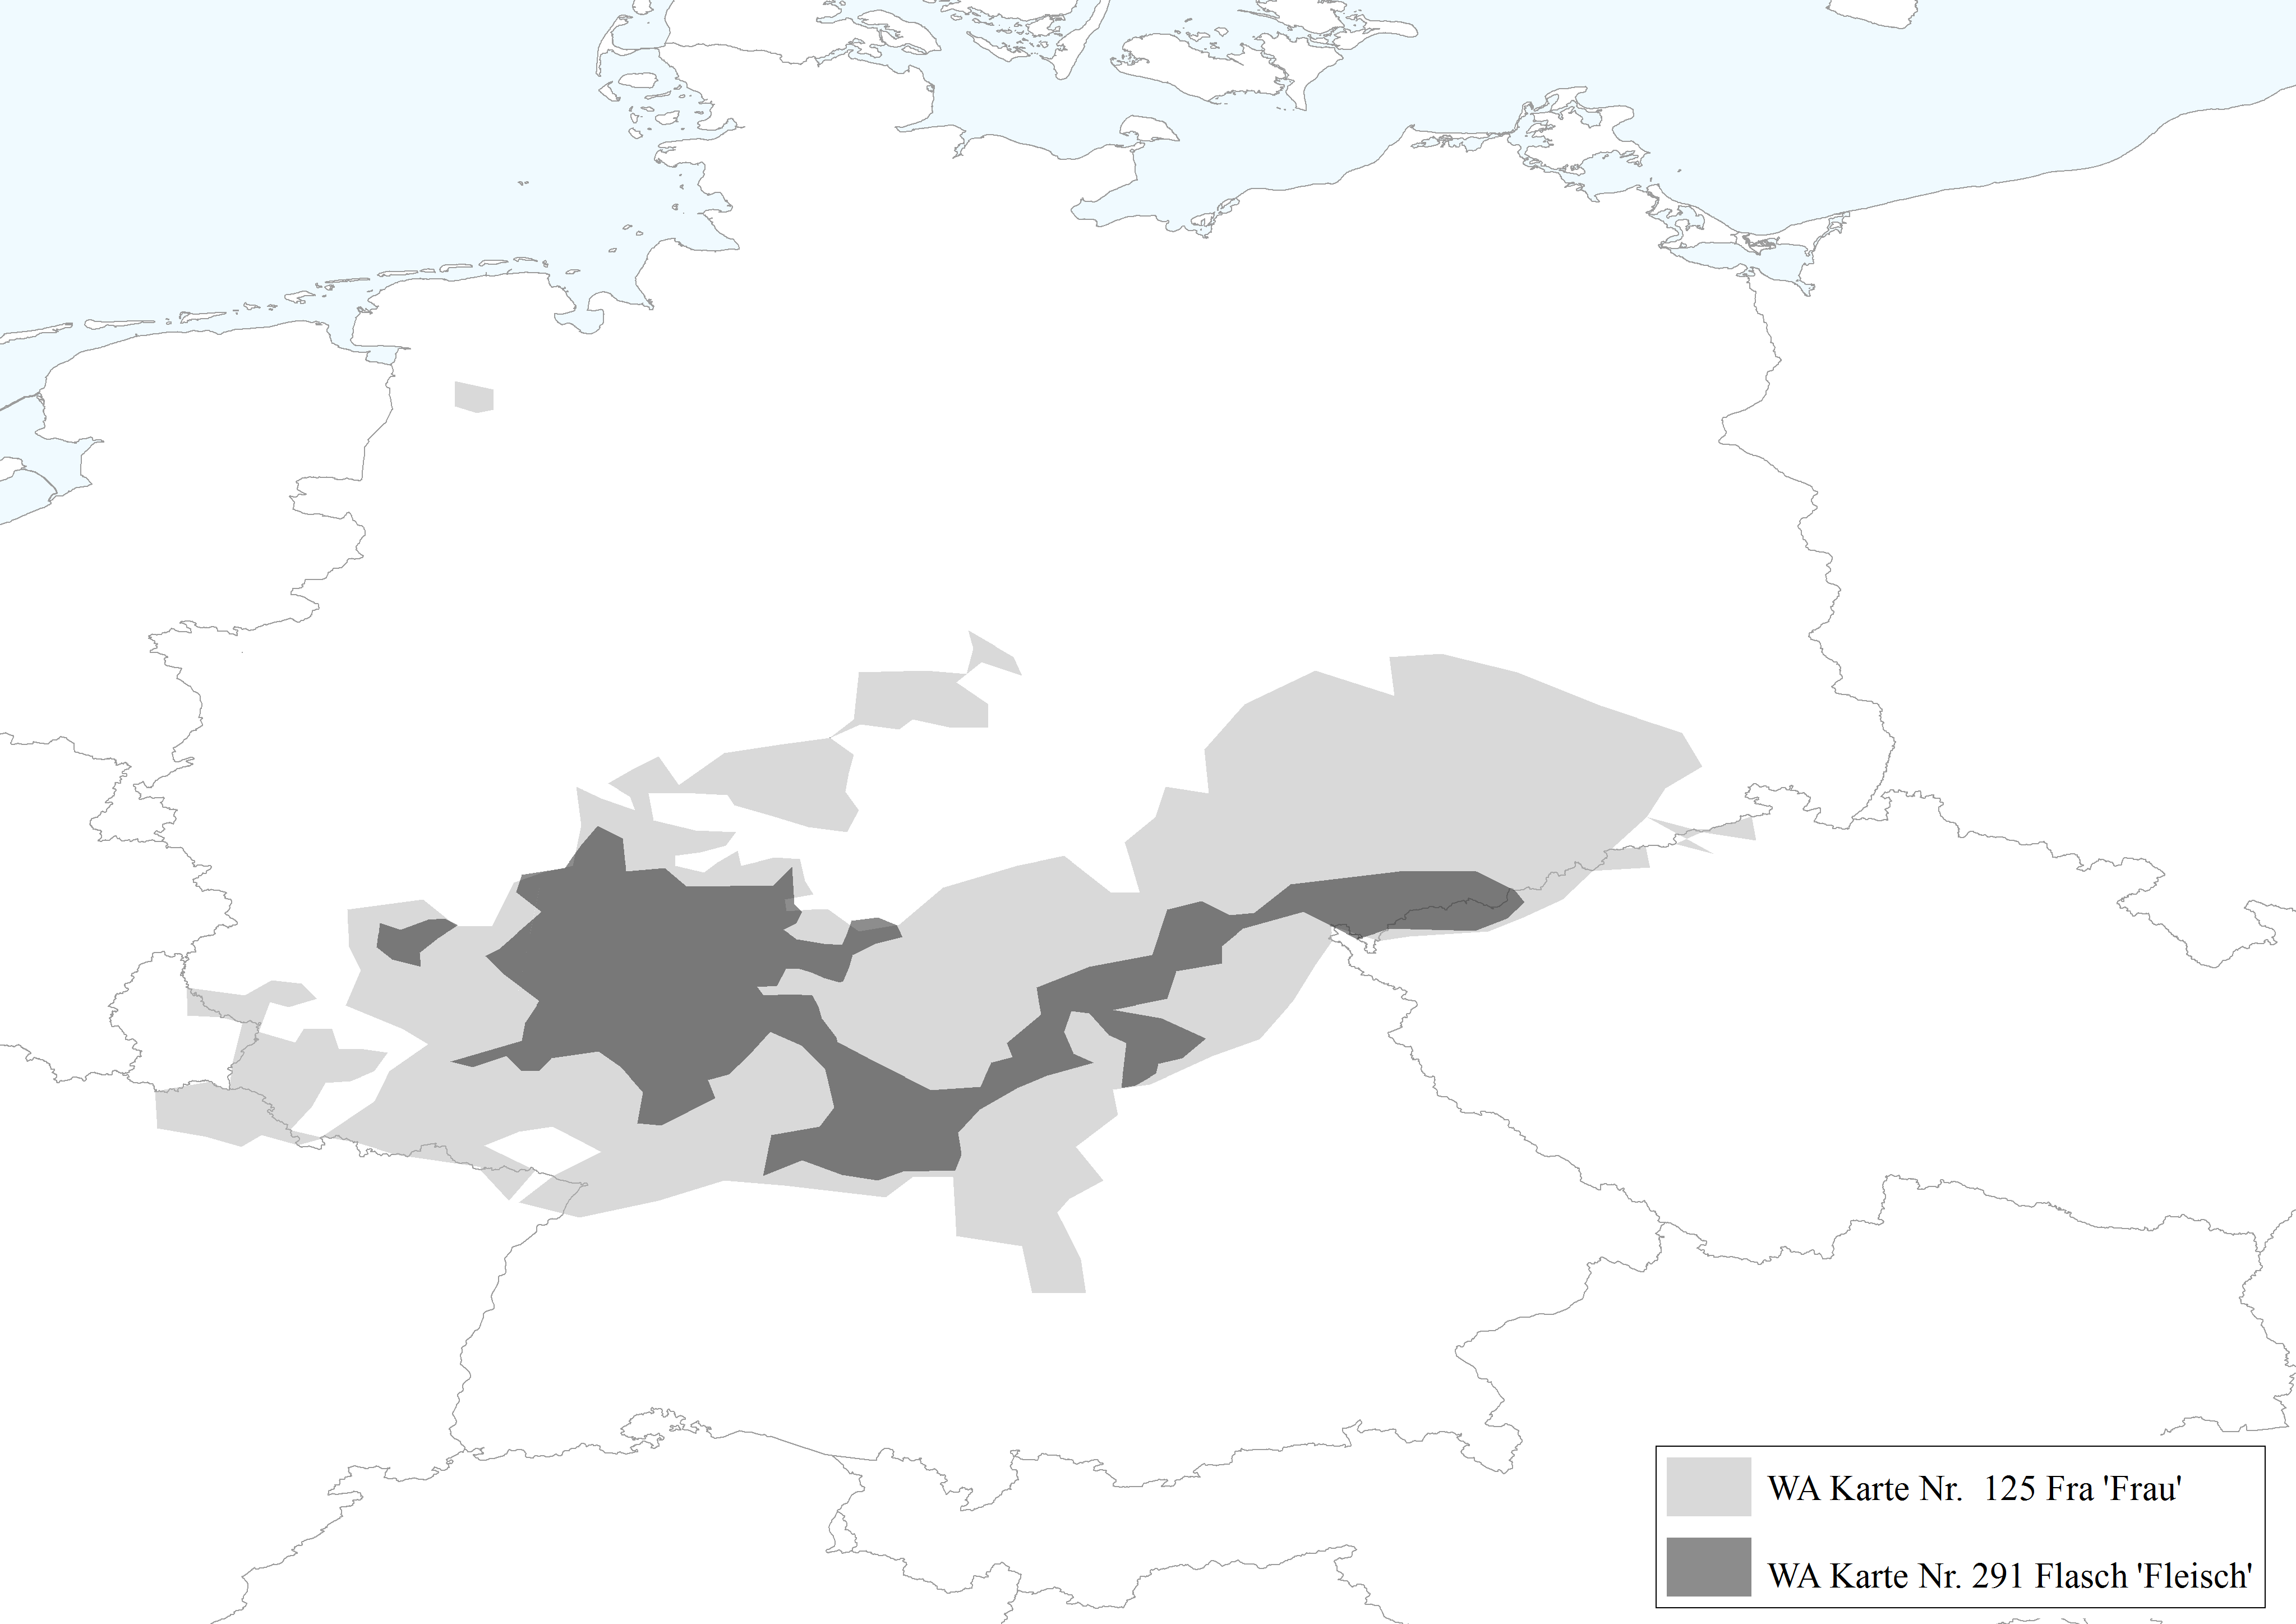
\includegraphics[scale=0.5]{figures/dteiou.png}
		\caption{\label{dteiou} Mhd. \textit{ou} u. \textit{ei} > /aː/ in den dt. Dialekten}
		\end{figure} 
\FloatBarrier
 
\subsection{\hai{V24} (\hai{E\textsubscript{4}}, mhd. \textit{ei})}\label{phonV24}
%  %\noindent
Zunächst zur Situation des historischen Diphthongs \hai{V24} (E\textsubscript{4}) < urj. *\textit{ej} im \hai{LiJi}. Eine Manipulation dieses Vokals findet sich im \hai{chrLiJi1}-Kernkorpus in 42 Texten. Damit weisen elf Texte keinerlei Markierung in dieser Position auf, d.\,h. hier findet sich ausschließlich ein als <ei> oder z.\,T. auch als <ey>, <ai>, <ay> wiedergegebener Diphthong, der dem Standarddeutschen gleicht. Von den 42 relevanten Texten tritt \hai{V24} als <a>, in 31 Texten längenmarkiert als <aa>  auf. Vier Texte zeigen außerdem eine Diphthongierung zu <oi>, <eu>; auch dieses Phänomen steht zum Teil parallel zu den gegebenen Monophthongen.  

Die geographische Streuung der Belege für eine Manipulation von mhd. \textit{ei} zeigt, dass wir den westjiddischen Monophthong in beinahe allen Regionen finden (vgl. Abb. \ref{karteV24DSA}). Eine Ausnahme bildet der äußerste Nordosten, wo keine bzw. nur eine diphthongische Manipulation vorliegt. Besonders viele Quellen mit dem westjiddischen Langvokal finden sich in Berlin, Leipzig, Bonn, Mannheim, Frankfurt und Wien.\footnote{Der Durchmesser der Diagramme in Abb. \ref{karteV24DSA} ist abhängig von der Anzahl der an diesem Ort relevanten Quellen.} Die Überblendung der Korpusdaten mit dem Areal von /\textit{a\textlengthmark}/ für mhd. \textit{ei} im Lexem \sem{Fleisch} in den deutschen Dialekten zeigt, dass zumindest an den Orten Frankfurt, Mannheim, Erlangen, Nürnberg und Wien ein Einwirken der deutschen Dialekte auf das \hai{chrLiJi1} nicht auszuschließen ist. \\
		
		\begin{figure}[h!]
		\centering
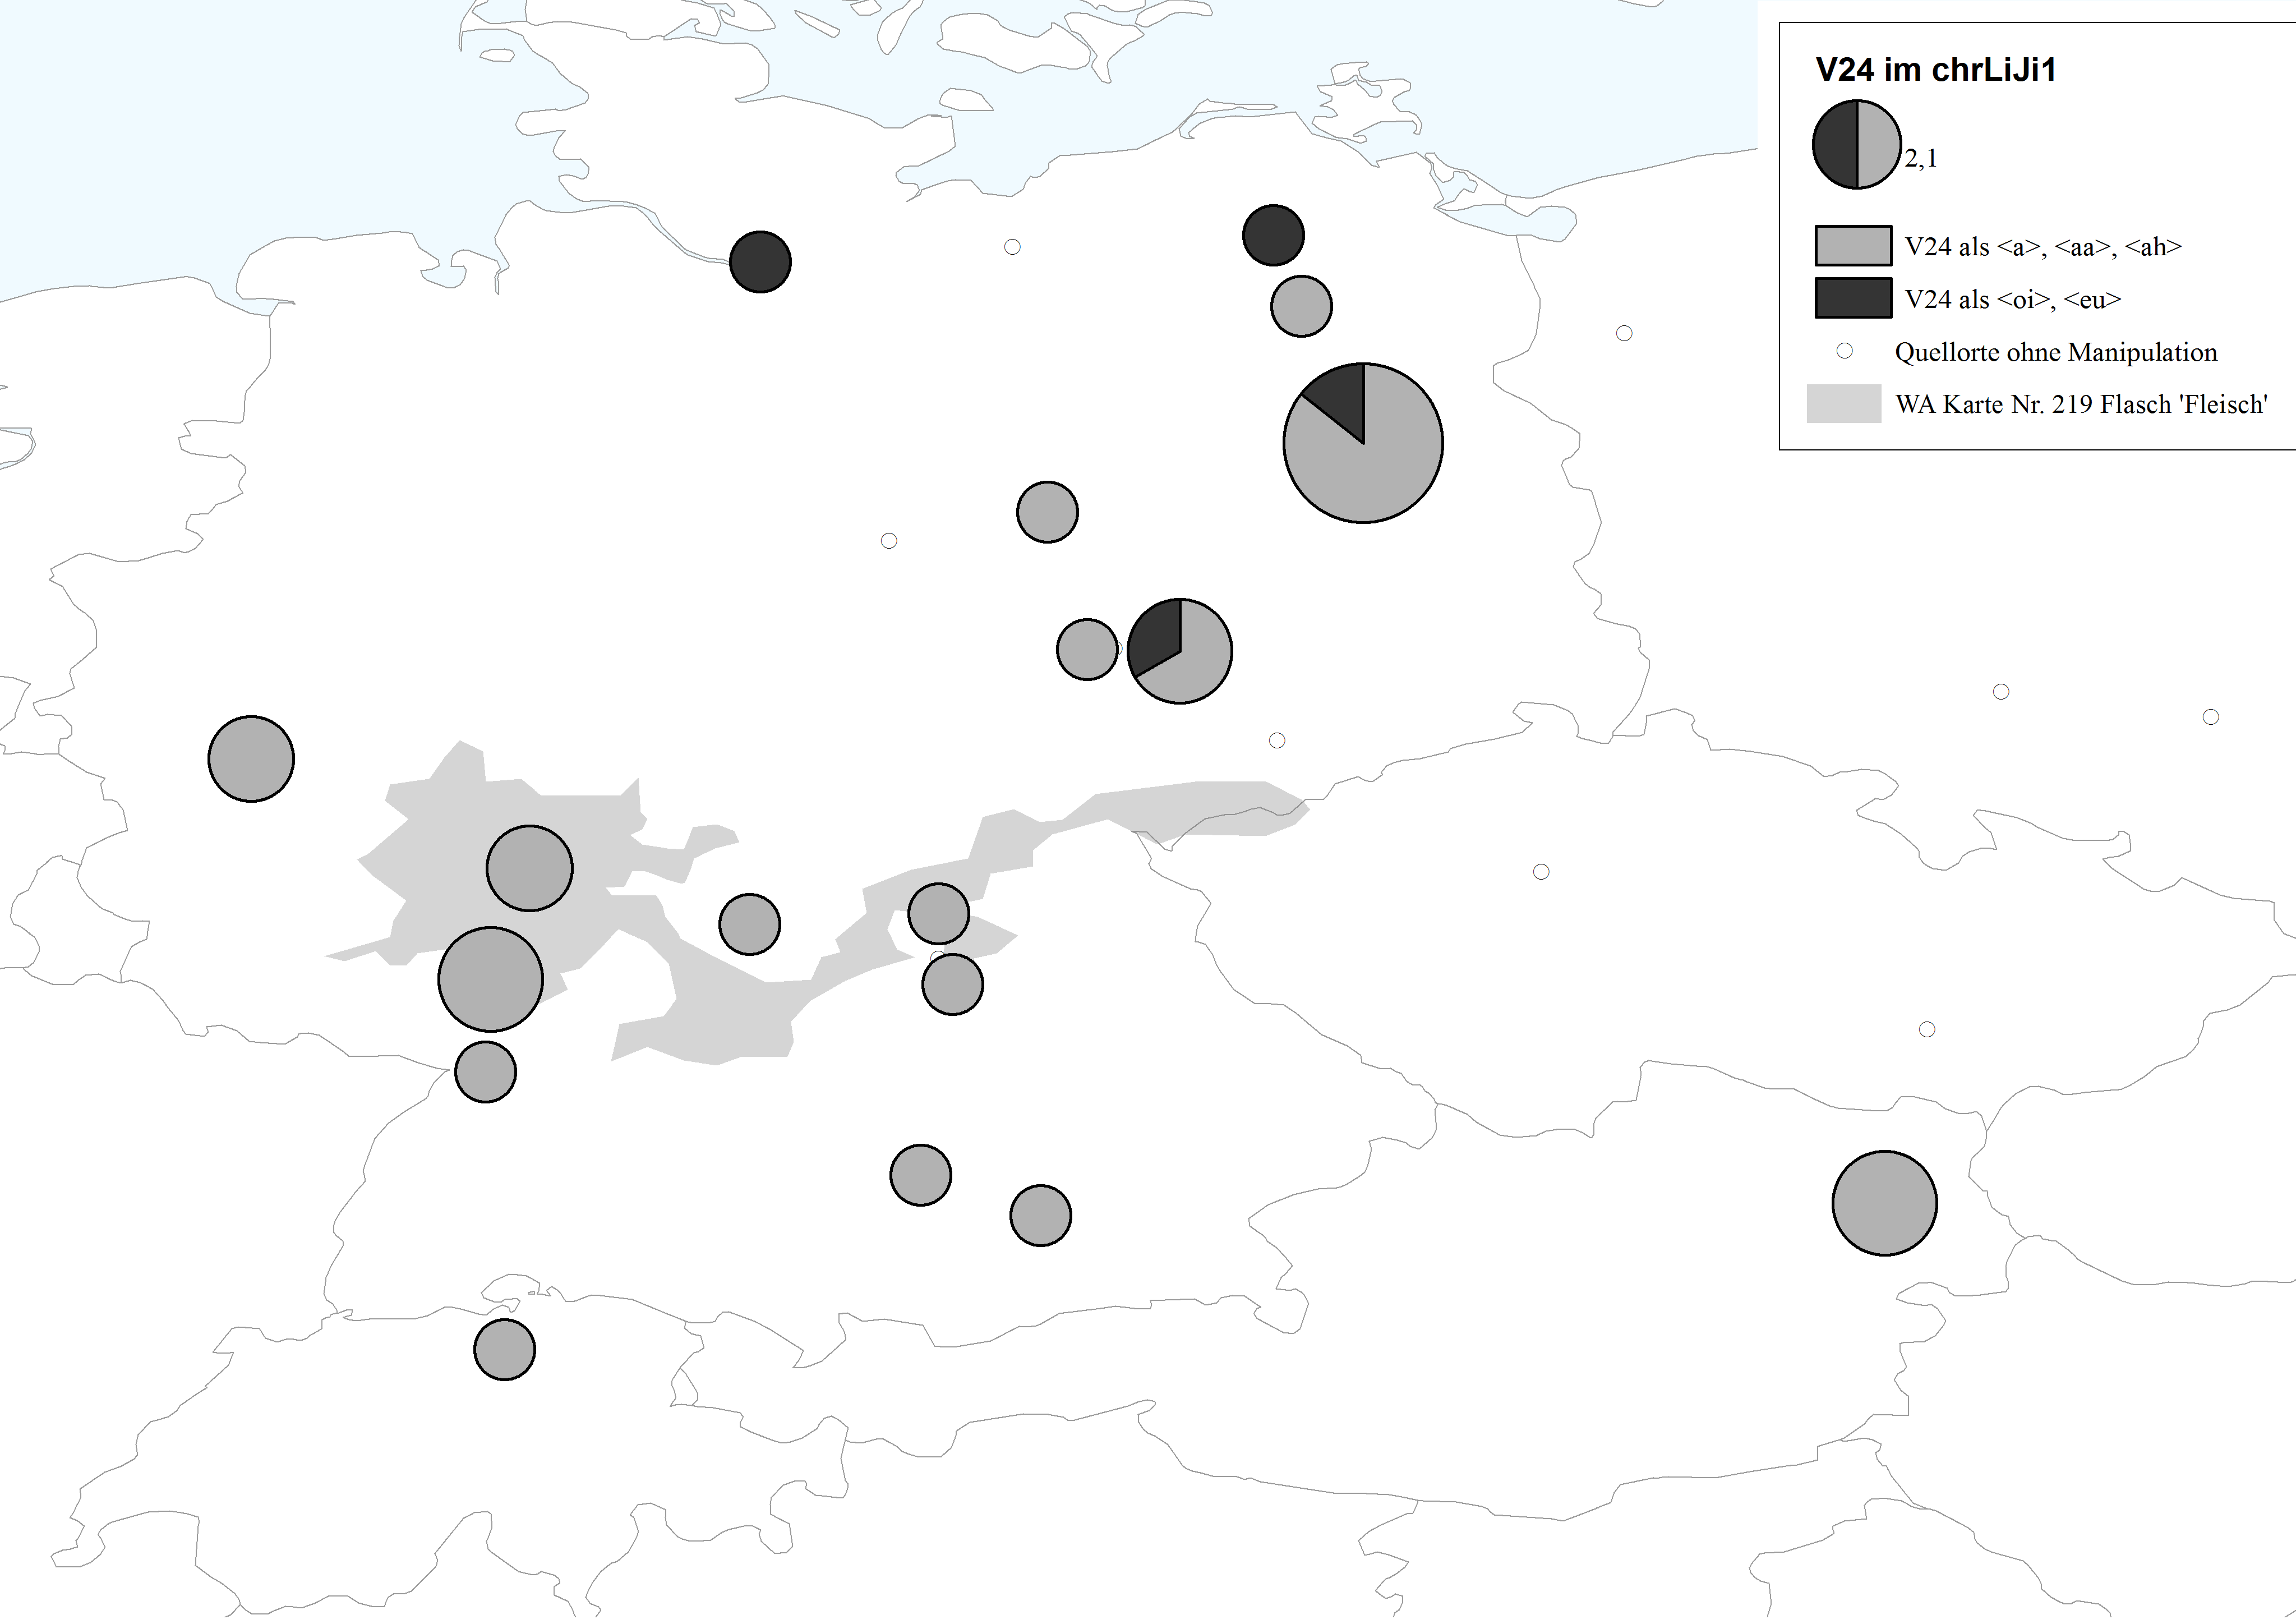
\includegraphics[scale=0.5]{figures/V24_neuDSA.png}
		\caption{\label{karteV24DSA}  \hai{V24} im \hai{chrLiJi1} mit WA Karte Nr. 291}
		\end{figure}
 \FloatBarrier


Die in der \hai{WA}-Karte nicht abgedeckten Dialekte der Schweiz und Österreichs zeigen gemäß der entsprechenden Karte des \hai{KDSA} Nr. 417, dass hier der mhd. Diphthong unverändert blieb. Die Monophthongierung zu /a\textlengthmark/ ist darin lediglich in einem burgenländischen Ort aufgeführt\footnote{Hinter diesem Ortspunkt könnte sich der westjiddische Wenkerbogen aus Frauenkirchen (\hai{WB} Nr. 42663) verbergen; der  \hai{KDSA} ist leider nicht transparent, welche Bögen in sein Sample einflossen.}. Tatsächlich ist die Monophthongierung von mhd. /ei/ > /a\textlengthmark/ aber in vielen modernen süd- und mittelbairischen Dialekten Österreichs belegt (vgl. \cite{Wiesinger2001}). \textcite[233]{Schirmunski1962} wie auch \textcite{Wiesinger2001} geben an, dass die Monophthongierung zu /a\textlengthmark/ < mhd. \textit{ei} besonders in \qu{Wien und andere[n] österreichische[n] Stadtmundarten} stattgefunden hat, also kein basisdialektales Phänomen darstellt. Für die hier relevante Wiener Standtmundart zeigt Wiesinger (\citeyear[92f]{Wiesinger2001}), dass bereits Ende des 19. Jahrhunderts der \qu{prestigeträchtige Wiener städtische[n] Monophthong} stark auf die Dialekte der niederösterreichische Landbevölkerung gewirkt hat. In Wien selbst ist ein Monophthong an der Position von mhd. \textit{ei} seit dem späten 12. Jh. belegt (vgl. \cite[113]{Wiesinger2001}). Die Wiener Quellen könnten demnach bei der Manipulation auf eine entsprechende Form im örtlichen deutschen Dialekt zurückgegriffen haben.
 
 Besonders interessant ist die Verteilung der Belege für <eu>, <oi> < mhd. \textit{ei}. Diese lassen sich mit keinem Einfluss der deutschen Mundarten erklären.\footnote{Ein entsprechender Diphthong /\textipa{\textopeno\textsubarch{I}}/ < mhd. \textit{ei} ist in den deutschen Dialekten nur im \ili{bairisch}-alemannischen Übergangsgebiet zu finden (vgl. \hai{WA} Karte Nr. 219).} Bei diesen Belegen ist zu vermuten, dass dieser Diphthong als Kennlaut für (Ost)jiddisch verwendet wurde, obwohl er in dieser Position keinerlei Entsprechung im Jiddischen hat.\footnote{Im \hai{OJ} unterscheidet sich \hai{V24} (mhd. \textit{ei}) als Diphthong [ej] nur wenig vom Schriftdeutschen.} Erstaunlich ist aber dennoch die durchaus gegebene Arealbildung von Quellen mit \hai{V24} als <eu>, <oi> im Nordosten. Da es keinen Grund dafür gibt, anzunehmen, dass diese Formen in irgendeiner Weise auf tatsächliche Sprachgegebenheiten referieren, ist zu vermuten, dass es sich hierbei um Hyperkorrekturen handelt, die den ostjiddischen Diphthong von \hai{V44} (mhd. \textit{ou}) und \hai{V42}/\,\hai{V43} (mhd. \textit{ô}) auf \hai{V24} übertragen. Dies ließe zwei weitere Schlüsse zu, die das Areal im Nordosten erklären: zum einen mag der Einfluss des Ostjiddischen in dieser Region stärker gewesen sein als andernorts,  zum anderen könnte die Unsicherheit bzw. Fehlerhaftigkeit bei der \isi{Imitation} des Jiddischen darauf schließen lassen, dass im Nordosten \ili{Westjiddisch} weniger vital war als im übrigen Untersuchungsgebiet. Für letztere Erklärung sprechen auch die Daten der diachronen Verteilung dieser Belege (Abb. \ref{V24}). Das Histogramm zeigt deutlich, dass der Diphthong <oi>, <eu> (/\textipa{\textopeno\textsubarch{I}}/) erst ab der zweiten Jahrhunderthälfte des 19. Jahrhunderts auftaucht, also zu einem Zeitpunkt, an dem der \isi{Sprachtod} des Westjiddischen bereits fortgeschritten war. Zwar finden sich noch authentische \hai{A1}-Quellen aus dem Nordosten für die erste Hälfte des 19. Jahrhunderts, wie etwa die Kindheitserfahrungen der Autobiographie A.\,H. Heymanns (1803–1880) aus Strausberg (Berlin) (vgl. \cite{Schaefer2013}), doch ab der zweiten Jahrhunderthälfte liegt kein authentisches Datum des \hai{A1}-Typs aus dieser Region vor.\footnote{Aus dem Nordwesten sind immerhin die recht jungen Quellen aus Aurich überliefert (Reershemius \citeyear{Reershemius2007}, \citeyear{Reershemius2014}).}
 
 Diachron streuen die Belege für den westjiddischen Monophthong von mhd. \textit{ei} sehr weit (s. Histogramm in Abbildung \ref{V24}). Den westjiddischen Langvokal finden wir überwiegend zwischen 1775 und 1870. Nach dieser Periode tritt dieses Phänomen zwar nur noch vereinzelt auf.  Auch fällt im diachronen Bild auf, dass Texte, welche auf eine Manipulation von mhd. \textit{ei} verzichten, leicht mit der Zeit abnehmen. Ab 1872 lässt sich  ein kurzzeitiger Einbruch von Belegen für den westjiddischen Monophthong erkennen. Insgesamt lässt sich dennoch festhalten, dass \hai{chrLiJi1} zwar nicht konsequent, aber überwiegend (in 31 von 53 Texten) den westjiddischen Langvokal einsetzt und damit die tatsächliche Sprachrealität wiedergibt.\\
 
 
 \begin{figure}[h!]
	\begin{tikzpicture}
		\begin{axis}[only marks, width=0.82\textwidth,height=0.2\textheight,
		legend style={at={(1,1)},xshift=+0.2cm, yshift=-0.25cm,anchor=north west,nodes=left},
			%title={Funktionstypen des sp\"aten Westjiddisch},
			xtick={1700, 1725, 1750, 1775, 1800, 1825, 1850, 1875, 1900, 1925, 1950, 1975}, ytick=\empty,
			x tick label style={/pgf/number format/1000 sep=}, 
			y tick label style={/pgf/number format/1000 sep=},
			%extra y ticks={456.1, 1022.4},
			%extra y tick labels={{456,1},{1022,4}},
			extra y tick style={grid=major,
				tick label style={, ,}},
				ymin=0.7,
				ymax=2,
			ylabel={Phänomenbelege},
			enlarge x limits=0.03]	
	
			
\addplot [mark=*, black] table [x=jahr, y=V24] {figures/V24a.txt}; %1.7
%\addplot [mark=*, gray] table [x=jahr, y=V24ae] {V24ae.txt}; %2
%\addplot [mark=square*, draw=black] table [x=jahr, y=V24e] {V24e.txt}; %1.7
\addplot [mark=*, gray] table [x=jahr, y=V24euoi] {figures/V24oi.txt}; %1.4
\addplot [mark=o, black] table [x=jahr, y=no] {figures/V24no_neu.txt}; %1.1

			% Andere Formen a={mark=square*,blue},% b={mark=triangle*,red},% c={mark=o,draw=black}}
						\legend{\hai{V24} als <a> , \hai{V24} als <oi>, unmanipuliert} %macht Legende
		\end{axis}
	\end{tikzpicture}
	\caption{\hai{V24} im \hai{chrLiJi1}}
	\label{V24}	
\end{figure}
\FloatBarrier


 \subsection{Der unbestimmte \isi{Artikel} als Sonderfall}\label{artikelkapitel}
%  %\noindent
 Eine Ausnahme bildet das Lexem des unbestimmten Artikels \sem{ein}, weil es sich aufgrund seiner hohen \isi{Frequenz} diachron wie diatopisch anders verhält als andere Lexeme, die einen aus mhd. \textit{ei} hervorgegangenen Vokal beinhalten.\footnote{Dem entsprechenden Eintrag im \textcite[Bd. 1, Sp. 520]{Lexer1992} zur Folge ist im Mittelhochdeutschen noch keine diatopische Variation zu erkennen.}   So wird dieses Lexem in 14 Quellen neben der Form \textit{a(n)} auch als \textit{ä(n)} oder \textit{e(n)} wiedergegeben.\footnote{Dies betrifft die Quellen \hai{AJ} (Berlin, 1825), \hai{DG} (Wien, 1858), \hai{FL} (Mannheim, 1778), \hai{GW} (n.a., ca. 1900), \hai{JK} (Breslau, 1810), \hai{LM} (Würzburg, 1844), \hai{MS} (Bonn, 1822), \hai{MV} (Berlin, 1862), \hai{NW} (Berlin, 1804), \hai{PF} (Augsburg, 1816), \hai{SS} (Berlin, 1907), \hai{SV} (München, 1890), \hai{TH} (Merseburg, 1820), \hai{VD} (Frankfurt, 1916).}. Doch gerade in diesem Lexem ist der Reduktionsvokal und selbst der \textit{n}-Ausfall auch in den deutschen Dialekten der Regelfall. So findet sich im Oberdeutschen verbreitet \textit{a}, im Mitteldeutschen \textit{e} und im Niederdeutschen \textit{e(n)} (vgl. \hai{WA} Karte Nr. 432). Hier kann demnach mehr die regionale Form auf das \hai{LiJi} gewirkt haben, als eine Orientierung am \hai{WJ}. Nach dem \hai{WjSA} (Karte Nr. 4) ist \textit{e} der unbestimmte \isi{Artikel} im gesamten Westjiddischen, während \textit{a} im Ostjiddischen und z.\,T. im niederländischen \hai{NWJ} verbreitet ist. Dieses Bild bestätigen die \hai{LiJi1}-Daten jedoch nicht. Auch der Blick auf authentische Quellen des \hai{WJ}, wo der unbestimmte \isi{Artikel} sehr wohl als \textit{a} belegt ist (Bsp. \ref{bspgrobein}–\ref{bsplevysein}), sprechen nicht für die Glaubwürdigkeit von Beraneks Kartenbild. \\

 \eenumsentence{
 \item \RL{א\makebox(-1.5,-7.5)[r]{\libertineGlyph{uni207B}}ה} \textit{ah} \sem{ein, einem, einen, eine, eines}\\
  (\qu{Die Hochzeit zu Grobsdorf} 1822:\,u.\,a. 1, 2, 6, 7, 10, 11) \label{bspgrobein}

 \item \RL{א\makebox(-1.5,-7.5)[r]{\libertineGlyph{uni207B}}} \textit{a} \sem{ein, einem, einen, eine, eines}\\
  (\qu{Esther. Oder die belohnte Tugend} Fürth, 1854:\,u.\,a. 1, 3, 4, 5, 7, 10) \label{bspestherein} 


 \item \textit{a} \sem{ein, einem, einen, eine, eines} \\
 (\qu{Grad wie bi's Lévy's} Mulhouse, 1928:\,u.\,a. 3, 4, 5, 6, 7, 10) \label{bsplevysein}  
 }
 
Die intertextuelle Unsicherheit und Variation lässt sich annähernd gut mit der geographischen Verteilung der Belege erklären. Die Karte in Abbildung \ref{karteV24e} zeigt, dass wir \textit{e(n)} \sem{ein} in nördlich verorteten Texten finden (mit einem Ausreißer in Wien), wo es auch die im Deutschen verbreitete Form darstellt. Im süddeutschen Gebiet, wo \textit{a(n)} \sem{ein} gebräuchlich ist, findet sich (von der bereits erwähnten Wiener Quelle abgesehen) kein Beleg für \textit{e(n)} im \hai{chrLiJi1}. Die Form des unbestimmten Artikels muss also durch die Situation im Deutschen beeinflusst worden sein. Viel interessanter als die Belege für \textit{e(n)} sind hingegen die Belege für \textit{a(n)} im Nordosten, wo diese Form in den deutschen Varietäten nicht gebräuchlich ist. Entweder sollten damit die oberdeutschen Eigenschaften des Jiddischen herausgestellt werden oder aber dies verweist tatsächlich auf eine weitere Verbreitung dieser Form als von Beraneck angenommen (vgl. \hai{WjSA} Karte Nr. 4).\footnote{Vgl. insbes. Bsp. \ref{bspgrobein}, wo sich \textit{a} \sem{ein} findet, obwohl dies im örtlichen zentralhessischen Dialekt nicht gegeben ist.}\\

	\begin{figure}[h!]
		\centering
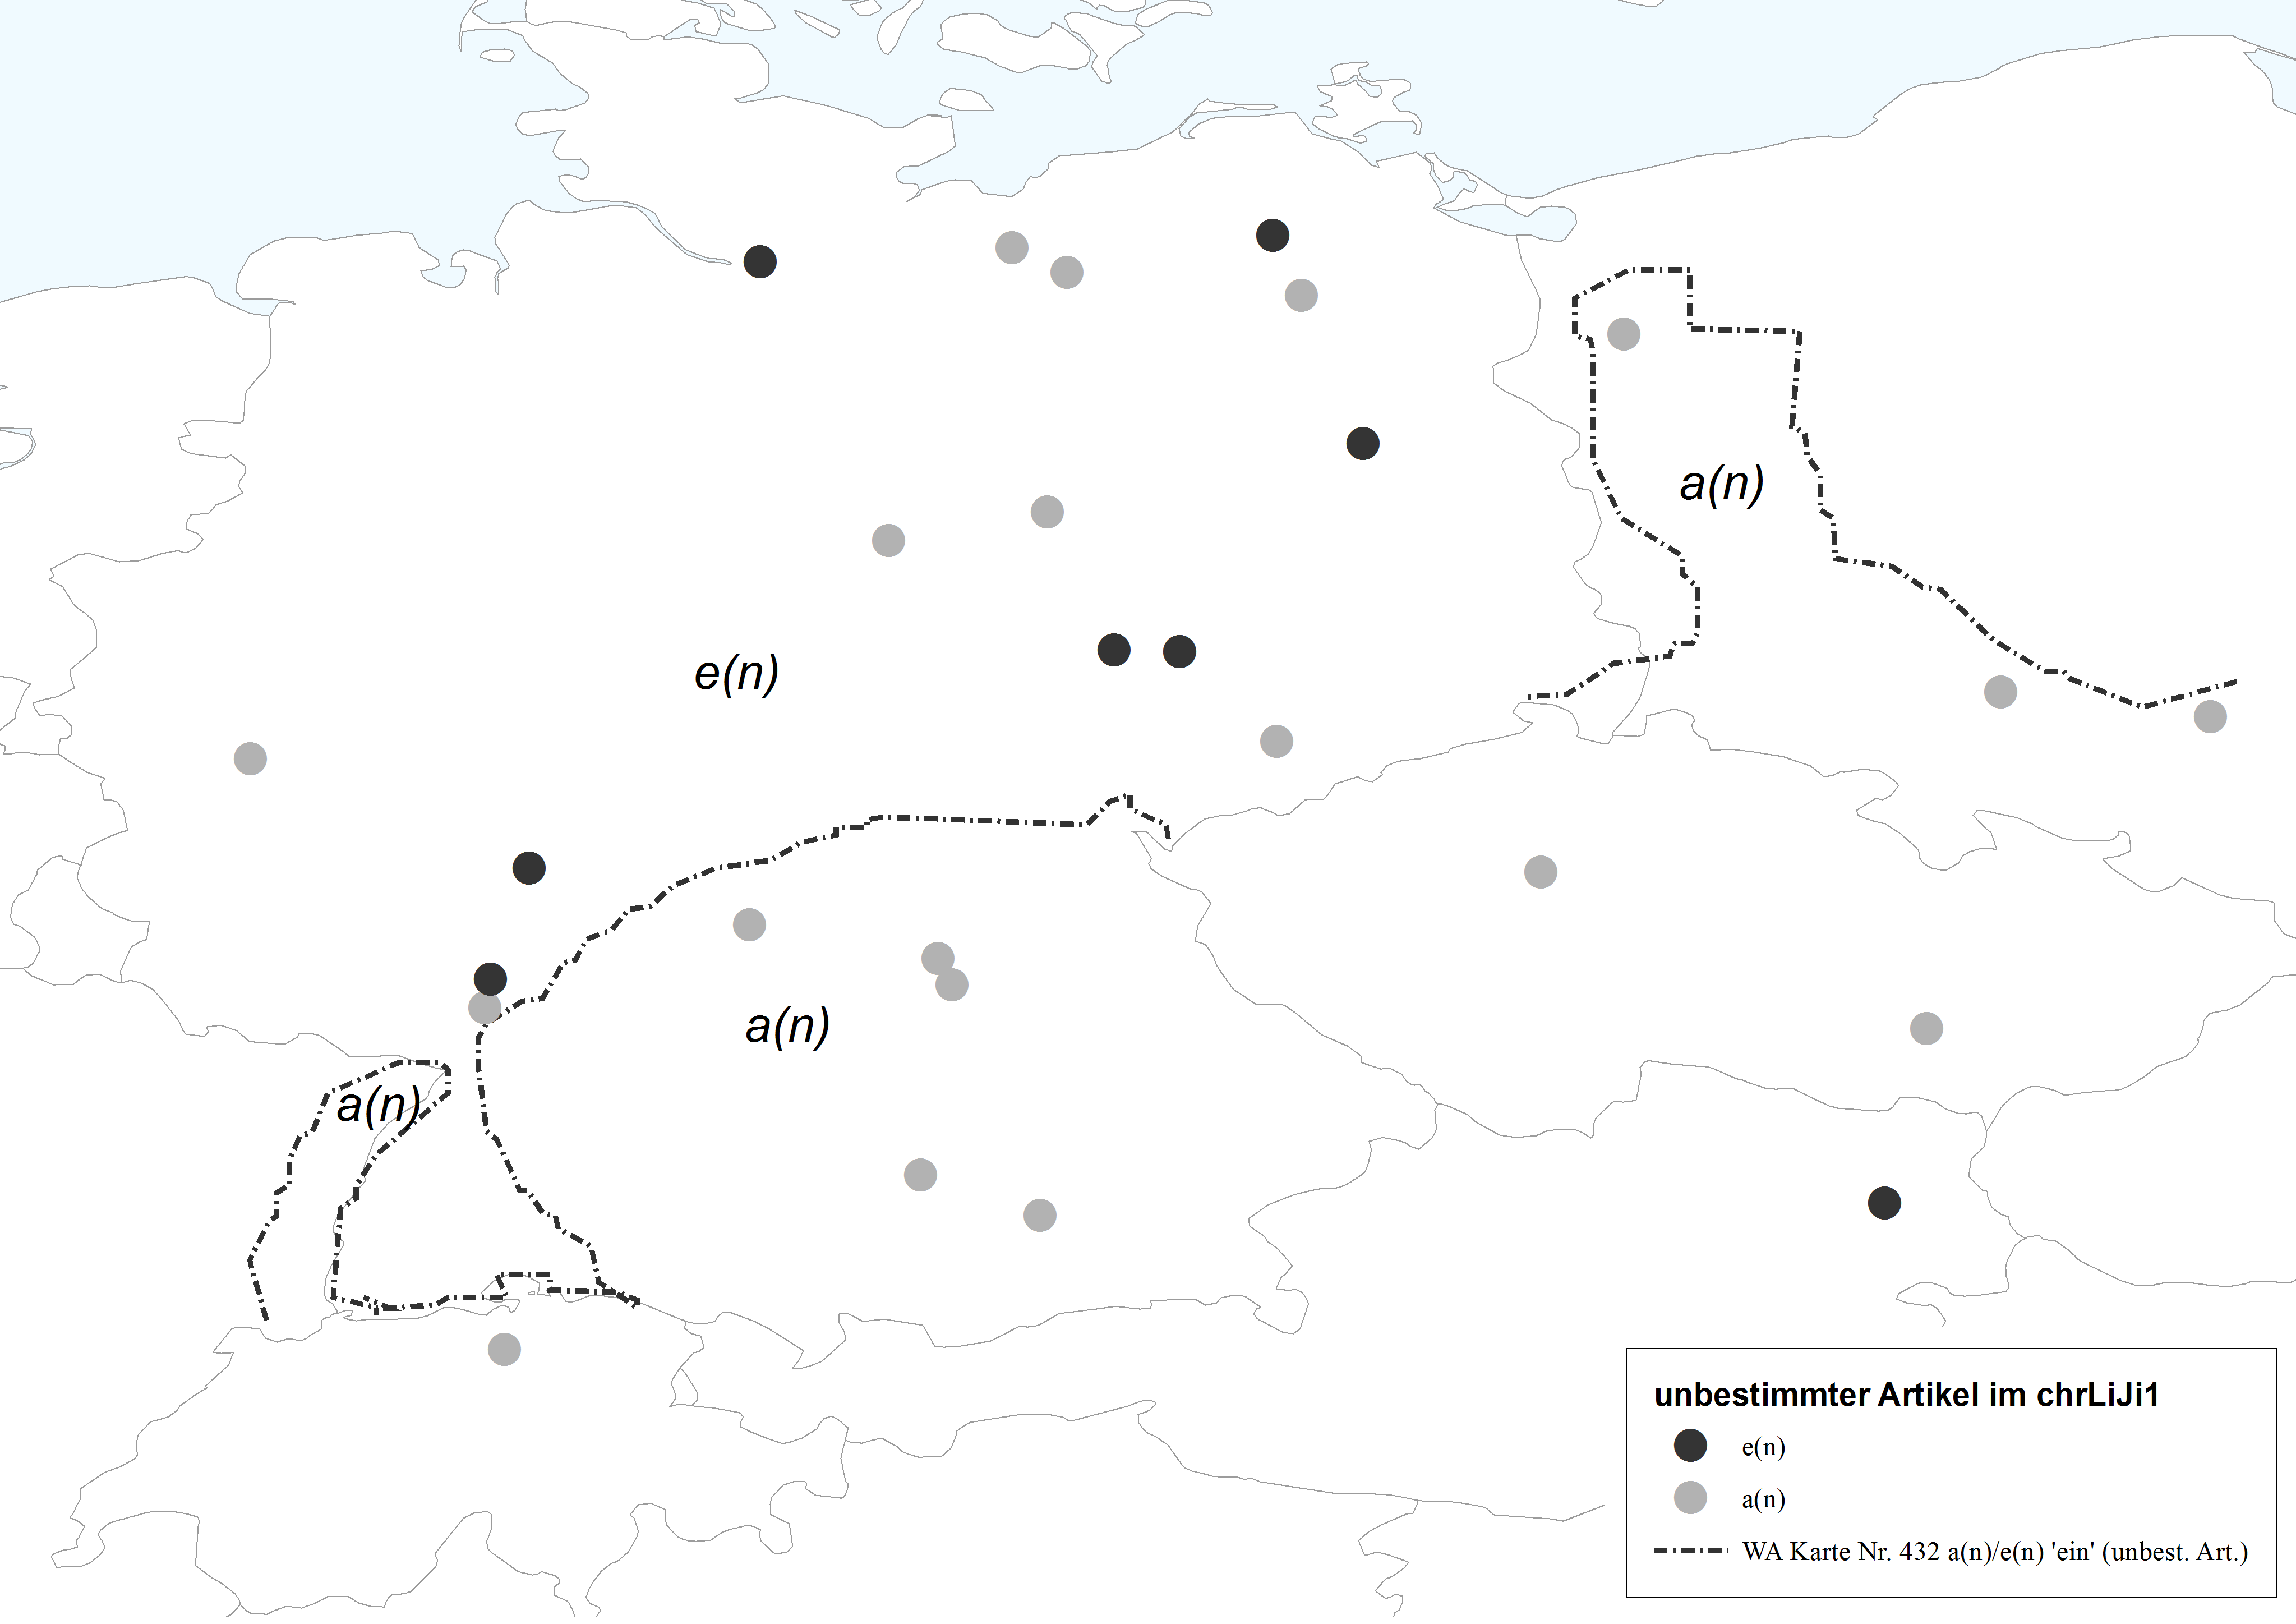
\includegraphics[scale=0.5]{figures/V24_ein_NEU.png}
		\caption{\label{karteV24e} Der unbestimmte \isi{Artikel} im \hai{chrLiJi1} mit WA Karte Nr. 432}
		\end{figure}
 \FloatBarrier
 
 
  \subsection{\hai{V24} im \hai{jüdLiJi1}}\label{liji2v24}
 %  %\noindent
In den Quellen des \hai{jüdLiJi1} findet sich die westjiddische Monophthongierung von \hai{V24} in neun von zehn Texten (s. Tabelle \ref{tblV24uedliji}). Auch hier gibt es eine gewisse Variation beim Vokal des unbestimmten Artikels: Nur zwei Texte (\hai{PBreslau} u. \hai{PDebrecen}) zeigen ausschließlich \textit{a(n)}, alle übrigen Quellen verwenden parallel \textit{e(n)} mit \textit{ä(n)}. 


 \begin{table}[h!]
\centering
		\begin{tabular}{lcc}
		\hline
	\textbf{Quelle} & \textbf{\hai{V24}  > /a\textlengthmark/ }& \textbf{unbest.} \textbf{Art.} \textbf{\textit{e(n)}}, \textbf{\textit{ä(n)}} \\ \hline % horizontale Trennlinie
\hai{GuS1}	&  \checkmark&	\checkmark	\\
\hai{GuS5}	&	\checkmark &	\checkmark	\\
\hai{GuS10}	&\checkmark&	\checkmark \\
 \hai{GuS15} &	–	&\checkmark\\	
\hai{GuS23}	&\checkmark&	\checkmark	\\
\hai{PAlsleben}	&	\checkmark&		\checkmark \\
\hai{PBerlin1}	&\checkmark&	\checkmark \\
\hai{PBerlin2}	&	\checkmark	&\checkmark \\
\hai{PBreslau}	&\checkmark&–\\	
\hai{PDebrecen}&	\checkmark&–\\	\hline
  \end{tabular} 
		 \caption{Modifikationen von \hai{V24} im \hai{JüdLiJi1}}
		 \label{tblV24uedliji}
		 \end{table}   
   

 \FloatBarrier
   
   
   \subsection{Hyperkorrekturen von nhd. /aɪ̯/ < mhd. (\textit{î} \hai{V34}, \hai{I\textsubscript{4}})}\label{hyperV24}
   %  %\noindent
   Jiddisch hat die sogenannte \quein{neuhochdeutsche Diphthongierung} von mhd. \textit{î}, \textit{iu}, \textit{û} und Monophthongierung von mhd. \textit{ie}, \textit{uo}, \textit{üe} vollständig mitgemacht  \parencite[14–18]{Timm1987}. Mhd. \textit{î} ist in weiten Teilen des Ostjiddischen und vollständig im Westjiddischen als Diphthong /aɪ̯/ belegt, nur im \hai{ZOJ} und \hai{SOJ} wurde der Diphthong wieder zu einem Monophthong /a\textlengthmark/, /a/ (vgl. \hai{LCAAJ} Karte Nr. 28; s.\,a. Karte in Abb. \ref{karteV34hyper}; s. Bsp. \ref{bspV34_1}–\ref{bspV34_4}).\footnote{An dieser Stelle sei darauf hingewiesen, dass das protojiddische Vokalsystem nach \textcite[161–205]{Herzog1965} die mittelhochdeutschen Langvokale \textit{î} und \textit{iu} zu ein- und demselben \qu{historischen Diphthong} urj. *\textit{əj:} zusammenfasst \parencite[1024]{Katz1983}. Da dieser Diphthong erst durch den \isi{Zusammenfall} von /\textit{i\textlengthmark}/ und /\textit{y\textlengthmark}/ im Zuge der \quein{neuhochdeutschen Diphthongierung} zwischen dem 12. und 16. Jahrhundert \parencite[146–149]{Koenig1978} zustande gekommen sein kann, das zusammengefallene Ergebnis kaum aber einen urjiddischen Zustand repräsentiert.} In den deutschen Dialekten ist mhd. \textit{î} lediglich in einem äußerst kleinen Gebiet des südwestlichen Moselfränkischen in wenigen Lexemen zu /a\textlengthmark/ geworden (vgl. \hai{WA} Karten Nr. 180, 176, 15) und ist damit eine sehr untypische Entwicklung im Deutschen.\\
   
    \eenumsentence{
    
    \item \hai{NWJ}:  \textit{gleich} \sem{gleich}  \\
    (\qu{Das verfrühte Schulenrufen} Aurich 1902:\,4. Auftritt [\cite[137]{Reershemius2007}]) \label{bspV34_1}
            
    \item \hai{ZWJ}: \RL{גלייך} \textit{gleykh} \sem{gleich}  \\
    (\qu{Die Hochzeit zu Grobsdorf} 1822:\,9) \label{bspV34_2}
    
    \item \hai{SWJ}: \textit{gleich} \sem{gleich} \\
    (\qu{Chateïsim sinn aach Laït} Mulhouse 1929:\,5) \label{bspV34_3}
    
    \item oj.: \RL{גל{יי}\makebox(-1.5,-7.5)[r]{\libertineGlyph{uni207B}}ך} \textit{glaykh}    \label{bspV34_4} 

    
    \item  mhd.: \textit{gelîch} (Lexer Bd. 1, Sp. 812) \label{bspV34} \label{bspV34_5}
    

    
    }
   
   
   
   In elf Quellen des \hai{chrLiJi1} findet sich neben der Monophthongierung von mhd. \textit{ei} (\hai{V24}) in einzelnen Lexemen die Monophthongierung von nhd. /aɪ̯/ in der Position von mhd. \textit{î} (\hai{V34}, \hai{I\textsubscript{4}}), wie z.\,B. in \ref{bsphyper1}–\ref{bsphyper3}. Bei diesen Belegen könnte es sich um Hyperkorrekturen handeln, da den Autoren die historischen Vokale kaum bewusst sein konnten und so die Monophthongierung von \hai{V24} (mhd. \textit{ei})  zu /a\textlengthmark/ als Regel für nhd. /aɪ̯/ angewandt wurde. Möglich wäre aber auch, dass diese Daten Ausdruck eines Reflexes aus dem \hai{ZOJ}/\hai{SOJ} durch Zuwanderung von Ostjiddischsprechern ins deutsche Sprachgebiet sind.\\ 
   
   
    \eenumsentence{
    
   \item \textit{blahb} \sem{bleibe} (\hai{DW} Wien, 1773:\,18) < mhd. \textit{blîben} \parencite[Bd. 1, Sp. 172]{Lexer1992} \label{bsphyper1}
   \item \textit{mahn} \sem{mein} (\hai{PA} Frankfurt, 1834:\,14, 51) < mhd. \textit{mîn} \parencite[Bd. 1, Sp. 2142]{Lexer1992} \label{bsphyper2}
   \item \textit{glach} \sem{gleich} (\hai{VE} Mannheim, 1784:\,62) < mhd. \textit{gelîch} \parencite[Bd. 1, Sp. 812]{Lexer1992}\label{bsphyper3}
    
    }
    
 
 Gegen einen ostjiddischen Einfluss spricht die historische Streuung der Daten (s. Abb. \ref{V34i}). <a>, <aa> findet sich besonders in den einhundert Jahren zwischen 1775 und 1875, tritt später aber nur mehr in einer Quelle (\hai{AK} Zürich, 1948) auf. Die Belege dieser Quelle, die generell relativ viele ostjiddische Merkmale aufweist, können zwar auf die zentralostjiddischen Formen zurückgeführt werden. Dadurch, dass aber kein Anstieg der ostjiddischen Formen im Verlauf des 19. Jahrhunderts zu verzeichnen ist, ist die Annahme, diese Belege seien durch ostjiddische Einwanderung und den \isi{Sprachtod} des Westjiddischen begünstigt, nicht bestätigt.\\


\begin{figure}[h!]
	\begin{tikzpicture}
		\begin{axis}[only marks, width=0.82\textwidth,height=0.2\textheight,
		legend style={at={(1,1)},xshift=+0.2cm, yshift=-0.5cm,anchor=north west,nodes=left},
			%title={Funktionstypen des sp\"aten Westjiddisch},
			xtick={1700, 1725, 1750, 1775, 1800, 1825, 1850, 1875, 1900, 1925, 1950, 1975}, ytick=\empty,
			x tick label style={/pgf/number format/1000 sep=}, 
			y tick label style={/pgf/number format/1000 sep=},
			%extra y ticks={456.1, 1022.4},
			%extra y tick labels={{456,1},{1022,4}},
			extra y tick style={grid=major,
				tick label style={, ,}},
				ymin=0.7,
				ymax=2.7,
			ylabel={Phänomenbelege},
			enlarge x limits=0.03]	
	
			

\addplot [mark=*, black] table [x=jahr, y=hyperV24] {figures/hyperv24dia.txt}; %2
\addplot [mark=o, black] table [x=jahr, y=no] {figures/hyperv24dia_no.txt}; %1

			% Andere Formen a={mark=square*,blue},% b={mark=triangle*,red},% c={mark=o,draw=black}}
						\legend{\hai{V34} (mhd. \textit{î}) als <a>, unmanipuliert} %macht Legende
		\end{axis}
	\end{tikzpicture}
	\caption{\hai{V34} (mhd. \textit{î}) im \hai{chrLiJi1}}
	\label{V34i}	
\end{figure}
\FloatBarrier
Die areale Verbreitung in Abbildung \ref{karteV34hyper}, spricht nicht eindeutig für einen Einfluss des Zentral- bzw. Südostjiddischen auf die Verwendung des Monophthongs an der Position von mhd. \textit{î}. Eine gewisse Affinität östlich verorteter Quellen (Wien, München, Leipzig, Berlin) zur ostjiddischen Form ist jedoch zu erkennen. Da es sich bei allen Quellorten, die diese Formen zeigen, um Großstädte handelt, und damit um Orte, an denen die ostjiddische Zuwanderung im 19. Jahrhundert besonders stark war (vgl. \cite{Lestschinsky1960}), spricht jedoch wiederum einiges dafür, dass hier tatsächlich das Ostjiddische der Migranten seine Spuren im \hai{LiJi1} hinterlassen hat. \\
    


 	\begin{figure}[h!]
		\centering
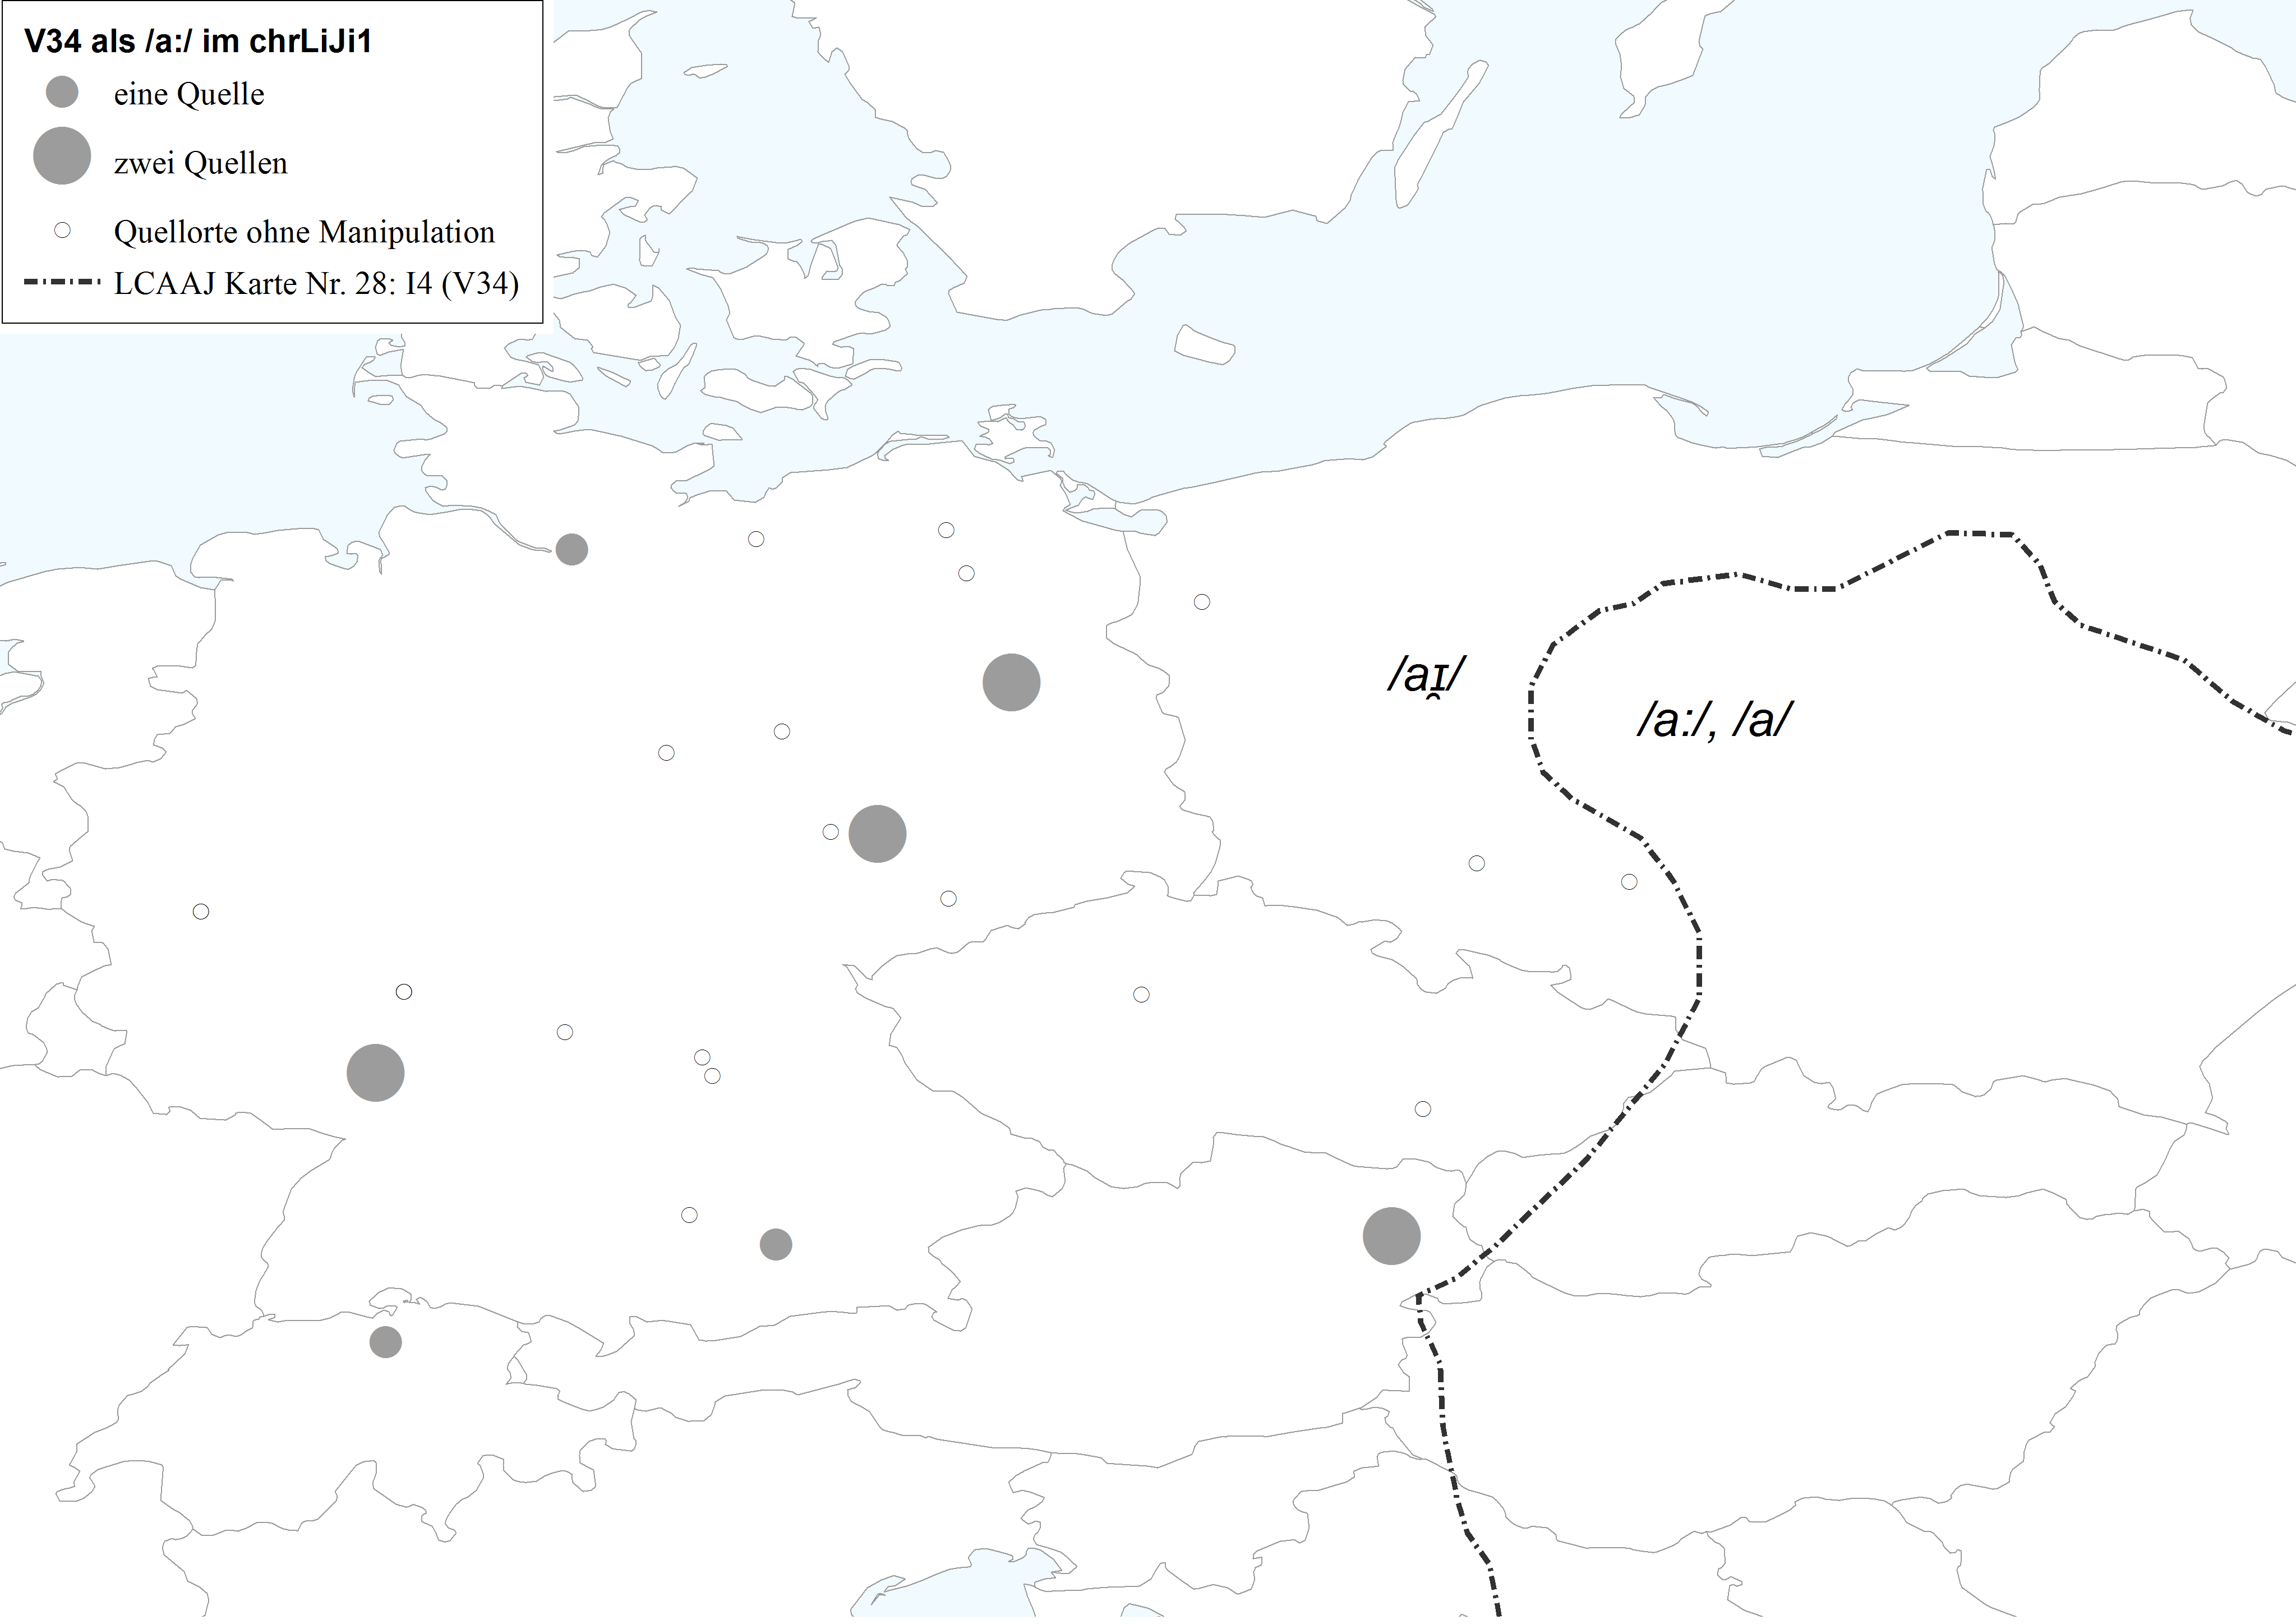
\includegraphics[scale=0.5]{figures/hyperV34_lcaaj.png}
		\caption{\label{karteV34hyper}  \hai{V34} als /a\textlengthmark/ im \hai{chrLiJi1} mit \hai{LCAAJ} Karte Nr. 28}
		\end{figure}
\FloatBarrier
 
Für einen Einfluss der ostjiddischen Dialekte sprechen besonders die Daten des \hai{jüdLiJi1}, in denen ein paar wenige solcher Formen in vier Quellen auftreten, vgl. Bsp. \ref{bspV34juedliji1}–\ref{bspV34juedliji4}.  Darunter finden sich zwei Quellen, die aus der näheren Kontaktzone zum Zentral- bzw. Südostjiddischen stammen. Der einfache Lösungsansatz bei den Belegen für mhd. \textit{î} als <a>, <aa> von einer Hyperkorrektur auszugehen, ist also nicht ohne weiteres zu bestätigen. Ein sich auf das Westjiddische auswirkender Einfluss des ostjiddischen Monophthongs ist jedoch in den authentischen Quellen des Westjiddischen nicht zu erkennen, s. Bsp.\ref{bspV34juedliji5}. Möglicherweise müssen wir bei unseren Belegen für /a\textlengthmark/ < mhd. \textit{î} eine Kombination aus ostjiddischem Dialekteinfluss und Hyperkorrektur annehmen. 


    \eenumsentence{
    \item \textit{saane} \sem{seine} (\hai{PAlsleben}:\,Titel, 4) \label{bspV34juedliji1}
    \item \textit{maan} \sem{meine} (\hai{PBreslau}:\,344) \label{bspV34juedliji2}
    \item \textit{was} \sem{weiß} (\hai{PDebrecen}:\,14) \label{bspV34juedliji3}
    \item \textit{maane}/\textit{mahne} \sem{meine} (\hai{GuS23}:\,10, 12) \label{bspV34juedliji4}
     \item \RL{גלייך}/\RL{גלייַך} \textit{gleykh}/\textit{glaykh} \sem{gleich} (\qu{Die Hochzeit zu Grobsdorf} 1822:\, u.\,a. 9, 14, 18) 
    \label{bspV34juedliji5}
    } 
    

 
   
   
 \subsection{\hai{V44} (\hai{O\textsubscript{4}}, mhd. \textit{ou})}\label{phonV44}
 %  %\noindent
30 von 53 Texten des \hai{chrLiJi1} weisen eine Manipulation von \hai{V44} (O\textsubscript{4}) < urj. *\textit{\textopeno j\textlengthmark} auf. 29 Texte zeigen dabei die Monophthongierung zu /a\textlengthmark/. Drei Texte zeigen, parallel zum Monophthong <a>, <aa> auch <o> in wenigen Lexemen auf.\footnote{Dies sind die Quellen \hai{DG} (Wien, 1858), \hai{JP} (Altona, 1867) u. \hai{WA} (Magdeburg, 1802) in \textit{lofen} \sem{laufen} (\hai{DG} Wien, 1858: 8), \textit{geglobt} \sem{geglaubt} (\hai{JP} Altona, 1867: 6R) u. \textit{globe} \sem{glaube} (\hai{WA} Magdeburg, 1802: 164).} Eine Quelle zeigt den Diphthong <äu>\footnote{Neben Belegen für den Monophthong /a\textlengthmark/ findet sich der Diphthong in \textit{gläuben} \sem{glauben} (\hai{AD} Leipzig, 1846: 137).} und eine weitere zeigt <oi>.\footnote{So belegt in der ostjiddischen Form \textit{oich} \sem{auch} (\hai{AK} Zürich, 1948: 219, 256).} 

Die diachrone Verteilung zeigt, dass der westjiddische Monophthong ab 1774 bis 1875 als Manipulationsstrategie weit verbreitet ist und zum Ende des 19. Jahrhunderts hin deutlich abnimmt (s. Histogramm in Abbildung \ref{V44}). \\



\begin{figure}[h!]
	\begin{tikzpicture}
		\begin{axis}[only marks, width=0.82\textwidth,height=0.2\textheight,
		legend style={at={(1,1)},xshift=+0.2cm, yshift=0cm,anchor=north west,nodes=left},
			%title={Funktionstypen des sp\"aten Westjiddisch},
			xtick={1700, 1725, 1750, 1775, 1800, 1825, 1850, 1875, 1900, 1925, 1950, 1975}, ytick=\empty,
			x tick label style={/pgf/number format/1000 sep=}, 
			y tick label style={/pgf/number format/1000 sep=},
			%extra y ticks={456.1, 1022.4},
			%extra y tick labels={{456,1},{1022,4}},
			extra y tick style={grid=major,
				tick label style={, ,}},
				ymin=0.7,
				ymax=2.7,
			ylabel={Phänomenbelege},
			enlarge x limits=0.03]	
	
			
\addplot [mark=*, black] table [x=jahr, y=a] {figures/V44a.txt}; %2.3
\addplot [mark=*, gray] table [x=jahr, y=o] {figures/V44o.txt}; %2
\addplot [mark=square*, draw=black] table [x=jahr, y=aeu] {figures/V44aeu.txt}; %1.7
\addplot [mark=triangle*, draw=black] table [x=jahr, y=oi] {figures/V44oi.txt}; %1.4
\addplot [mark=o, black] table [x=jahr, y=no] {figures/V44no.txt}; %1.1

			% Andere Formen a={mark=square*,blue},% b={mark=triangle*,red},% c={mark=o,draw=black}}
						\legend{\hai{V44} als <a>/ , \hai{V44} als <o>, \hai{V44}  als <äu>, \hai{V44} als <oi>, unmanipuliert} %macht Legende
		\end{axis}
	\end{tikzpicture}
	\caption{\hai{V44} im \hai{chrLiJi1}}
	\label{V44}	
\end{figure}
\FloatBarrier
 
 
 Im Vergleich zu den Manipulationsstrategien von \hai{V24} (s. Unterabschnitt \ref{phonV24}) treten im \hai{V44}-Kontext deutlich weniger Alternativen zu /a\textlengthmark/ auf. 
 Dies könnte damit erklärt werden, dass dieser Monophthong in der Entwicklung aus mhd. \textit{ou} auch in den deutschen Mundarten deutlich weiter verbreitet ist als der aus mhd. \textit{ei} (vgl. Karte \ref{dteiou}). 

 Mit Blick auf die areale Verbreitung der Manipulationen von \hai{V44} und der Situation von mhd. \textit{ou} in den deutschen Dialekten (s. Karte in Abbildung \ref{karteV44DSA}),\footnote{Die Situation im Schweizer und österreichischen Alemannisch sowie im österreichischen Bairisch gestaltet sich nach der entsprechenden Karte des \hai{KDSA} Nr. 425, so, dass hier überwiegend der standarddeutsche Diphthong /a\textsubarch{u}/ auftritt bzw. im Bodensee- und Höchstalemannischen der mhd. Diphthong unverändert blieb. Eine Monophthongierung zu  /a\textlengthmark/ ist in den Karten des \hai{KDSA} nicht verzeichnet. Nach \textcite[235]{Schirmunski1962} findet sich im \qu{Bairisch-österreichischen […] langes ā vor -m, bisweilen vor Lippenlauten überhaupt, z. B.: Inn. bām \sem{Baum}, lāb \sem{Laub}, aber āu \sem{Auge}}. Besonders für den Wiener Stadtdialekt, 
   der für unser \isi{Korpus} eine Rolle spielt, gilt dies (vgl. \cite[60–63]{SchusterSchikola1956}; \cite[33]{Bacciocco1890}). Damit sind die \hai{chrLiJi1}-Belege für /a\textlengthmark/ der Wiener Quellen auch auf eine regional verbreitete Form zurückzuführen.} fällt auf, dass überwiegend im /a\textlengthmark/-Areal der deutschen Dialekte und in dessen unmittelbarer Nachbarschaft auch im \hai{chrLiJi1} der westjiddische Vokal auftritt. Ausnahmen bilden die Quellen im Brandenburgischen und in Hamburg, wo keine Nähe zu einem deutschen Dialekt gegeben ist, der einen entsprechenden Wandel zeigt.\\
 
 

 	
		\begin{figure}[h!]
		\centering
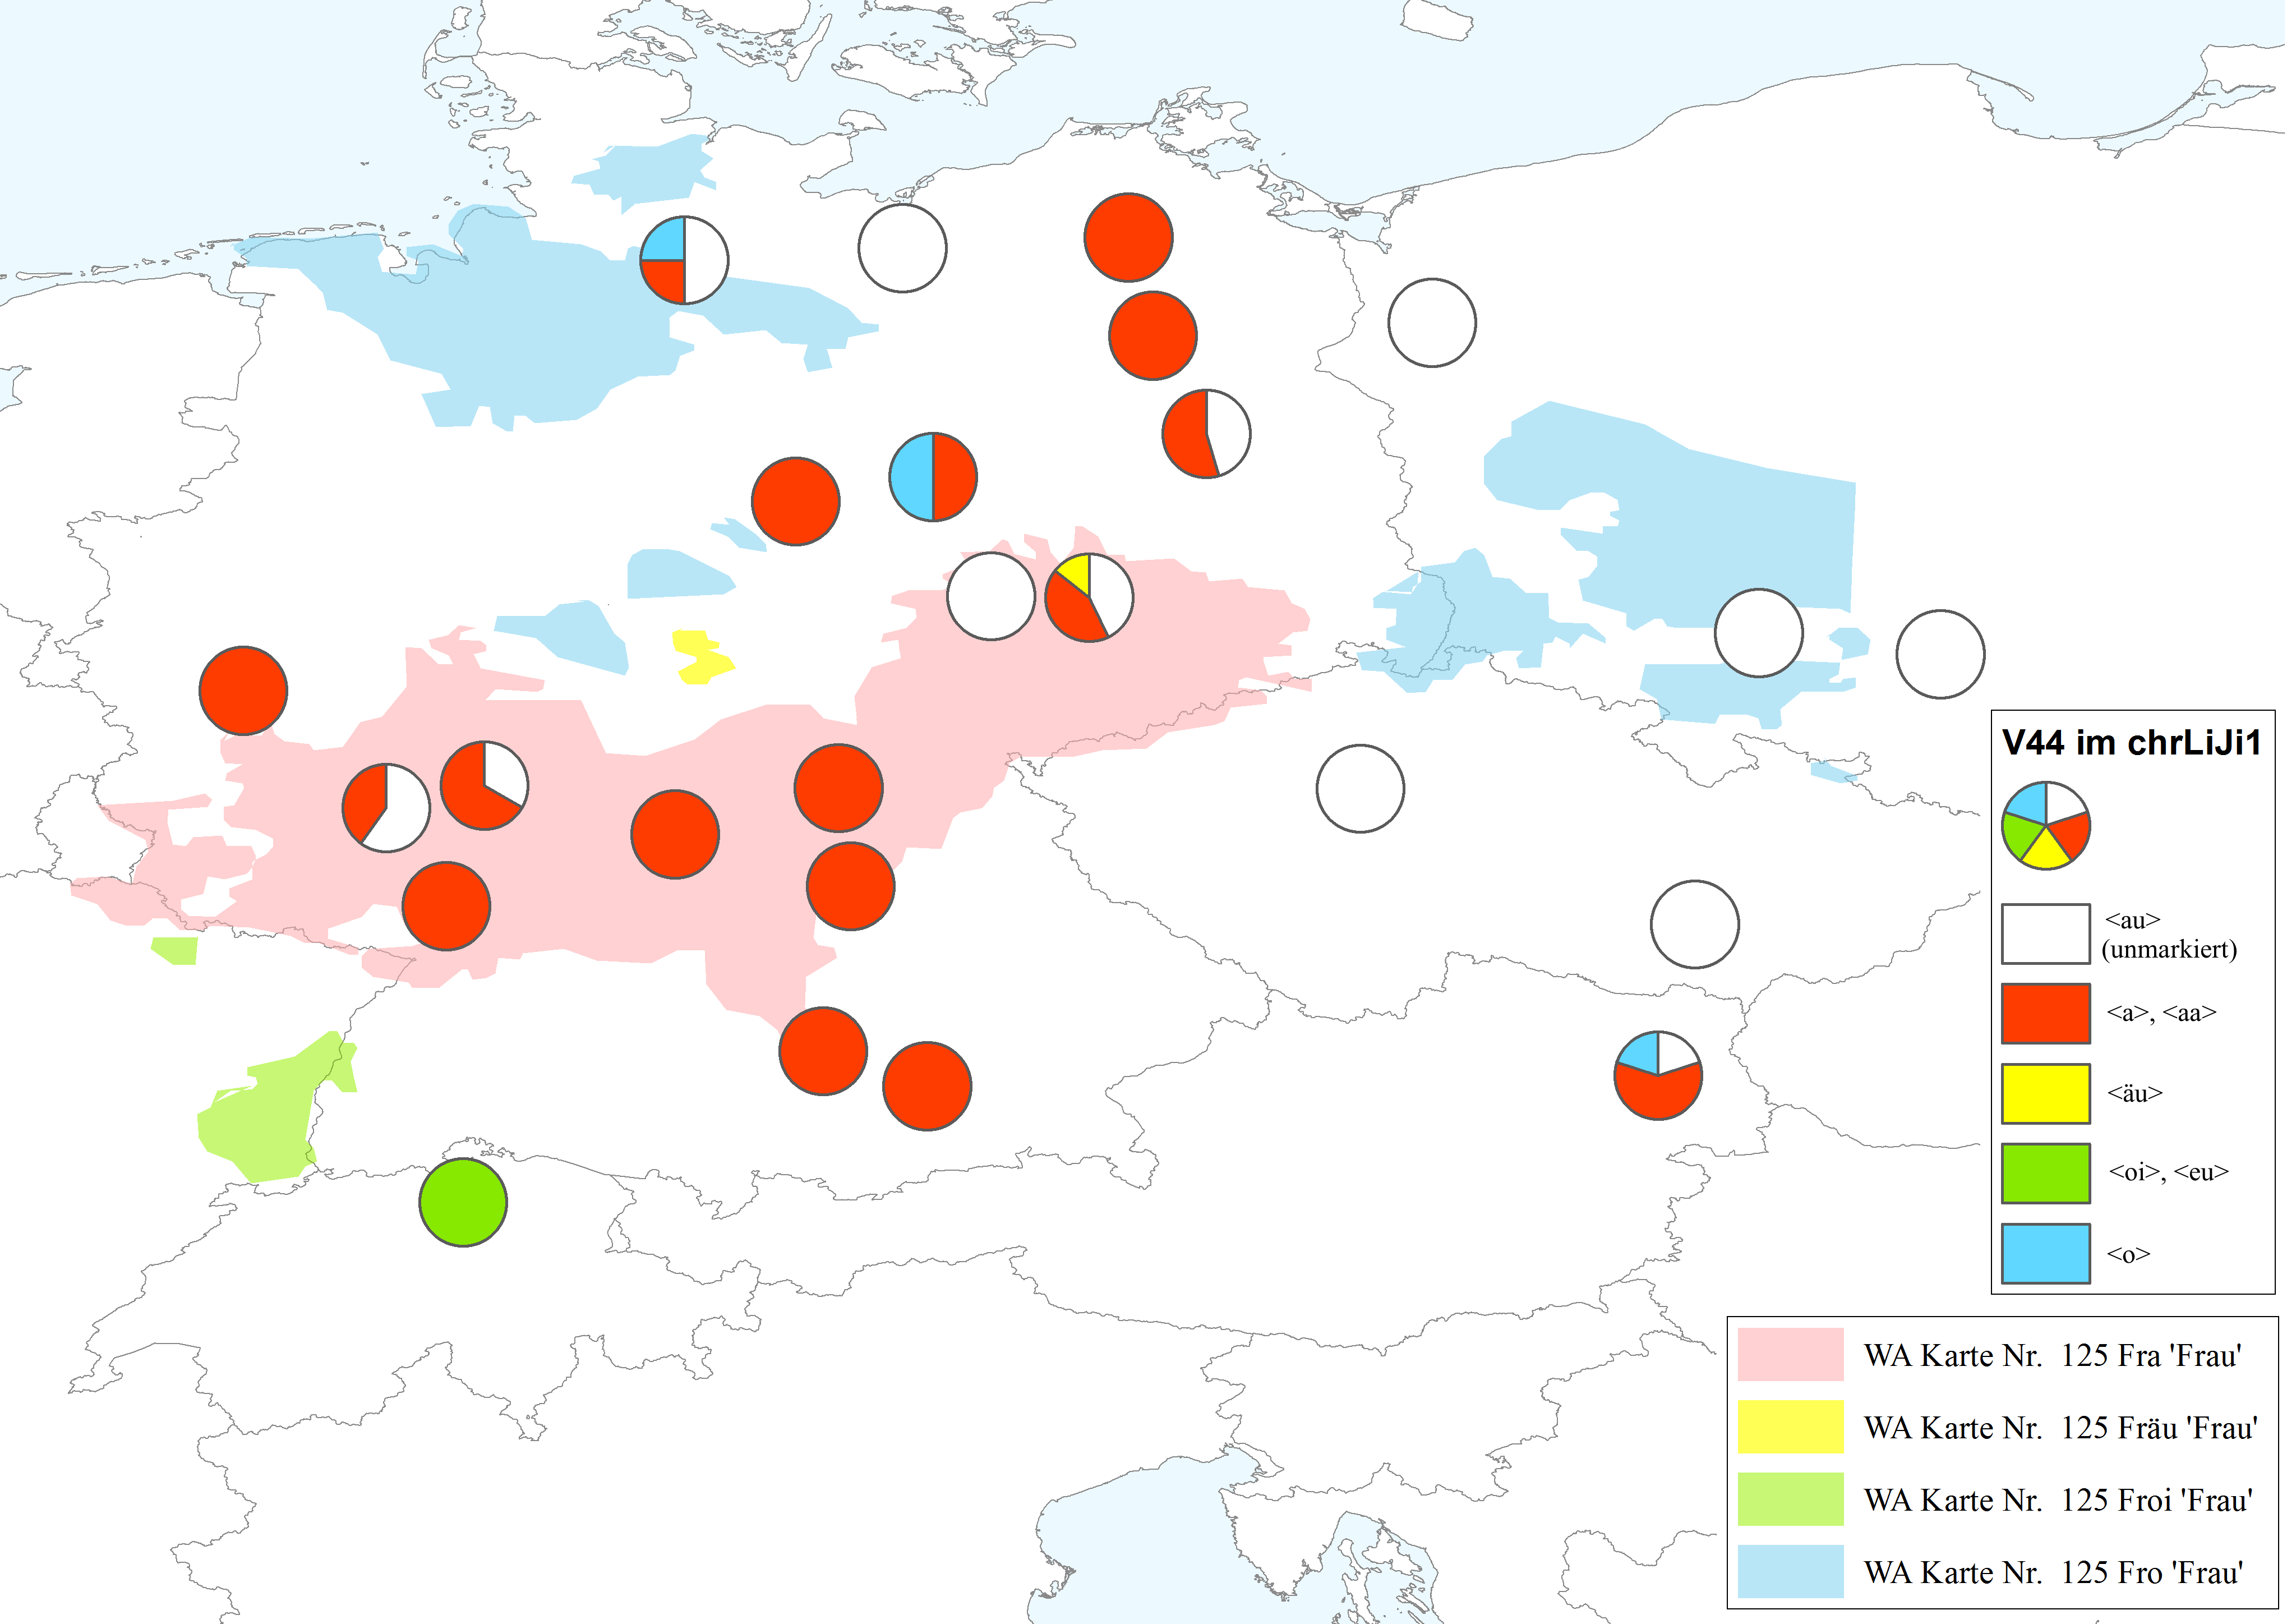
\includegraphics[scale=0.1]{figures/V44allDSA.png}
		\caption{\label{karteV44DSA}  \hai{V44} im \hai{chrLiJi1} mit WA Karte Nr. 125}
		\end{figure}
\FloatBarrier
 
 Die Situation im \hai{jüdLiJi1} zeigt ein ähnliches Bild. In allen Quellen überwiegt  die Monophthongierung von mhd. \textit{ou} >  /a\textlengthmark/: vier der fünf Pamphlete weisen den westjiddischen Langvokal auf. Jedoch nur zwei der fünf \hai{GuS} zeigen den Monophthong. \hai{PBreslau} zeigt neben <a> eine Verdumpfung des Monophthongs zu <o> in \textit{weggelofen} \sem{weggelaufen} (\hai{PBreslau}:\, 340) und \textit{loof} \sem{lauf} (\hai{PBreslau}:\,342). In demselben Lemma findet sich diese Manipulation zu <o> auch in \hai{PBerlin1} \textit{geloffen} \sem{gelaufen} (\hai{PBerlin1}:\,3, 5, 6) und \hai{GuS5} \textit{geloffen} \sem{gelaufen} (\hai{GuS5}:\,4), hier jedoch ohne weitere Belege der westjiddischen Form. Auch \hai{PBerlin2} weist ausschließlich Belege für <o> auf, z.\,B.  \textit{Ogen} \sem{Augen} (\hai{PBerlin2}:\,1.Sp.), \textit{geglobt} \sem{geglaubt} (\hai{PBerlin2}:\,1.Sp.).


 \subsection{\isi{Zusammenfall} von \hai{V24} und \hai{V44} > /a\textlengthmark/}\label{V24V44}
 %  %\noindent
Ein idiosynkratisches Phänomen des \hai{WJ} ist nicht allein die Monophthongierung der Vokale \hai{V24} und \hai{V44}, sondern der \isi{Zusammenfall} zweier historischer Diphthonge zu einem Langvokal. Lediglich 16 der 53 Quellen im \hai{chrLiJi1}-\isi{Korpus} weisen diesen Wandel beider Vokale zu /a\textlengthmark/ auf.\footnote{Diese Quellen sind \hai{AO} (Wien, 1770), \hai{BW} (Leipzig, 1826), \hai{DG} (Wien, 1858), \hai{FE} (Leipzig, 1792), \hai{GP} (Nürnberg, 1831), \hai{GW} (n.a., ca. 1900), \hai{IA} (Erlangen, 1840), \hai{LB} (Berlin,  1785), \hai{LS} (Bonn, 1925), \hai{MS} (Bonn, 1822), \hai{NW} (Berlin, 1804), \hai{PF} (Augsburg,  1816), \hai{PM} (Magdeburg, 1792), \hai{SV} (München, 1890), \hai{VD} (Frankfurt, 1916) und \hai{WA} (Magdeburg, 1802).} Wie das Histogramm zeigt (s. Abb. \ref{V24V44bild}), findet sich dieser \isi{Zusammenfall} sogar bis in die 1920er hinein und ist damit länger im \hai{chrLiJi1} belegt, als viele ein vitales \hai{WJ} annehmen.\footnote{Die drei Quellen des 20. Jh. sind \hai{GW} (n.a., ca. 1900), \hai{VD} (Frankfurt, 1916) und \hai{LS} (Bonn, 1925).} Ab 1870 lässt sich allerdings ein Trend erkennen, dass dieses Phänomen nur noch sporadisch im \hai{chrLiJi1} auftritt.\\
 
  %%%V24 und V44Diagramm%\begin{flushleft}	
\begin{figure}[h!]
	\begin{tikzpicture}
		\begin{axis}[only marks, width=0.82\textwidth,height=0.2\textheight,
		legend style={at={(1,1)},xshift=+0.2cm, yshift=-0.4cm,anchor=north west,nodes=left},
			%title={Funktionstypen des sp\"aten Westjiddisch},
			xtick={1700, 1725, 1750, 1775, 1800, 1825, 1850, 1875, 1900, 1925, 1950, 1975}, ytick=\empty,
			x tick label style={/pgf/number format/1000 sep=}, 
			y tick label style={/pgf/number format/1000 sep=},
			%extra y ticks={456.1, 1022.4},
			%extra y tick labels={{456,1},{1022,4}},
			extra y tick style={grid=major,
				tick label style={, ,}},
				ymin=0.7,
				ymax=3.4,
			ylabel={Phänomenbelege},
			enlarge x limits=0.03]	
\addplot [mark=square*, draw=black]  table [x=jahr, y=zusammenfall] {figures/V24V44.txt}; %2.3			
\addplot [mark=*, fill=white] table [x=jahr, y=V24] {figures/V24a2.txt}; %2		
\addplot [mark=square*, fill=white]  table [x=jahr, y=a] {figures/V44a2.txt}; %1.3


			% Andere Formen a={mark=square*,blue},% b={mark=triangle*,red},% c={mark=o,draw=black}}
						\legend{\hai{V24} u. \hai{V44} <a>, \hai{V24} als <a>, \hai{V44} als <a>}
		\end{axis}
	\end{tikzpicture}
	\caption{\hai{V24} und \hai{V44} im \hai{chrLiJi1}}
	\label{V24V44bild}	
\end{figure}
\FloatBarrier
 
 Erstaunlich ist ebenfalls die räumliche Verteilung der Quellen, in denen der westjiddische \isi{Zusammenfall} umgesetzt wurde. Lediglich eine Quelle stammt aus dem Gebiet, in dem der \isi{Zusammenfall} auch in den deutschen Mundarten gegeben ist. Zwei weitere Quellen liegen zumindest in nächster Nähe zum Gebiet des Zusammenfalls. Alle übrigen Quellen liegen in Gebieten, in denen kein \isi{Zusammenfall} stattgefunden hat (s. Abbildung \ref{karteV24V44}). Eine Ausnahme bilden wohl die Wiener Quellen, da hier ebenfalls z.\,T. ein \isi{Zusammenfall} > /a\textlengthmark/stattgefunden hat (vgl. \cite[233, 235]{Schirmunski1962}).\\
 
 \begin{figure}[h!]
		\centering
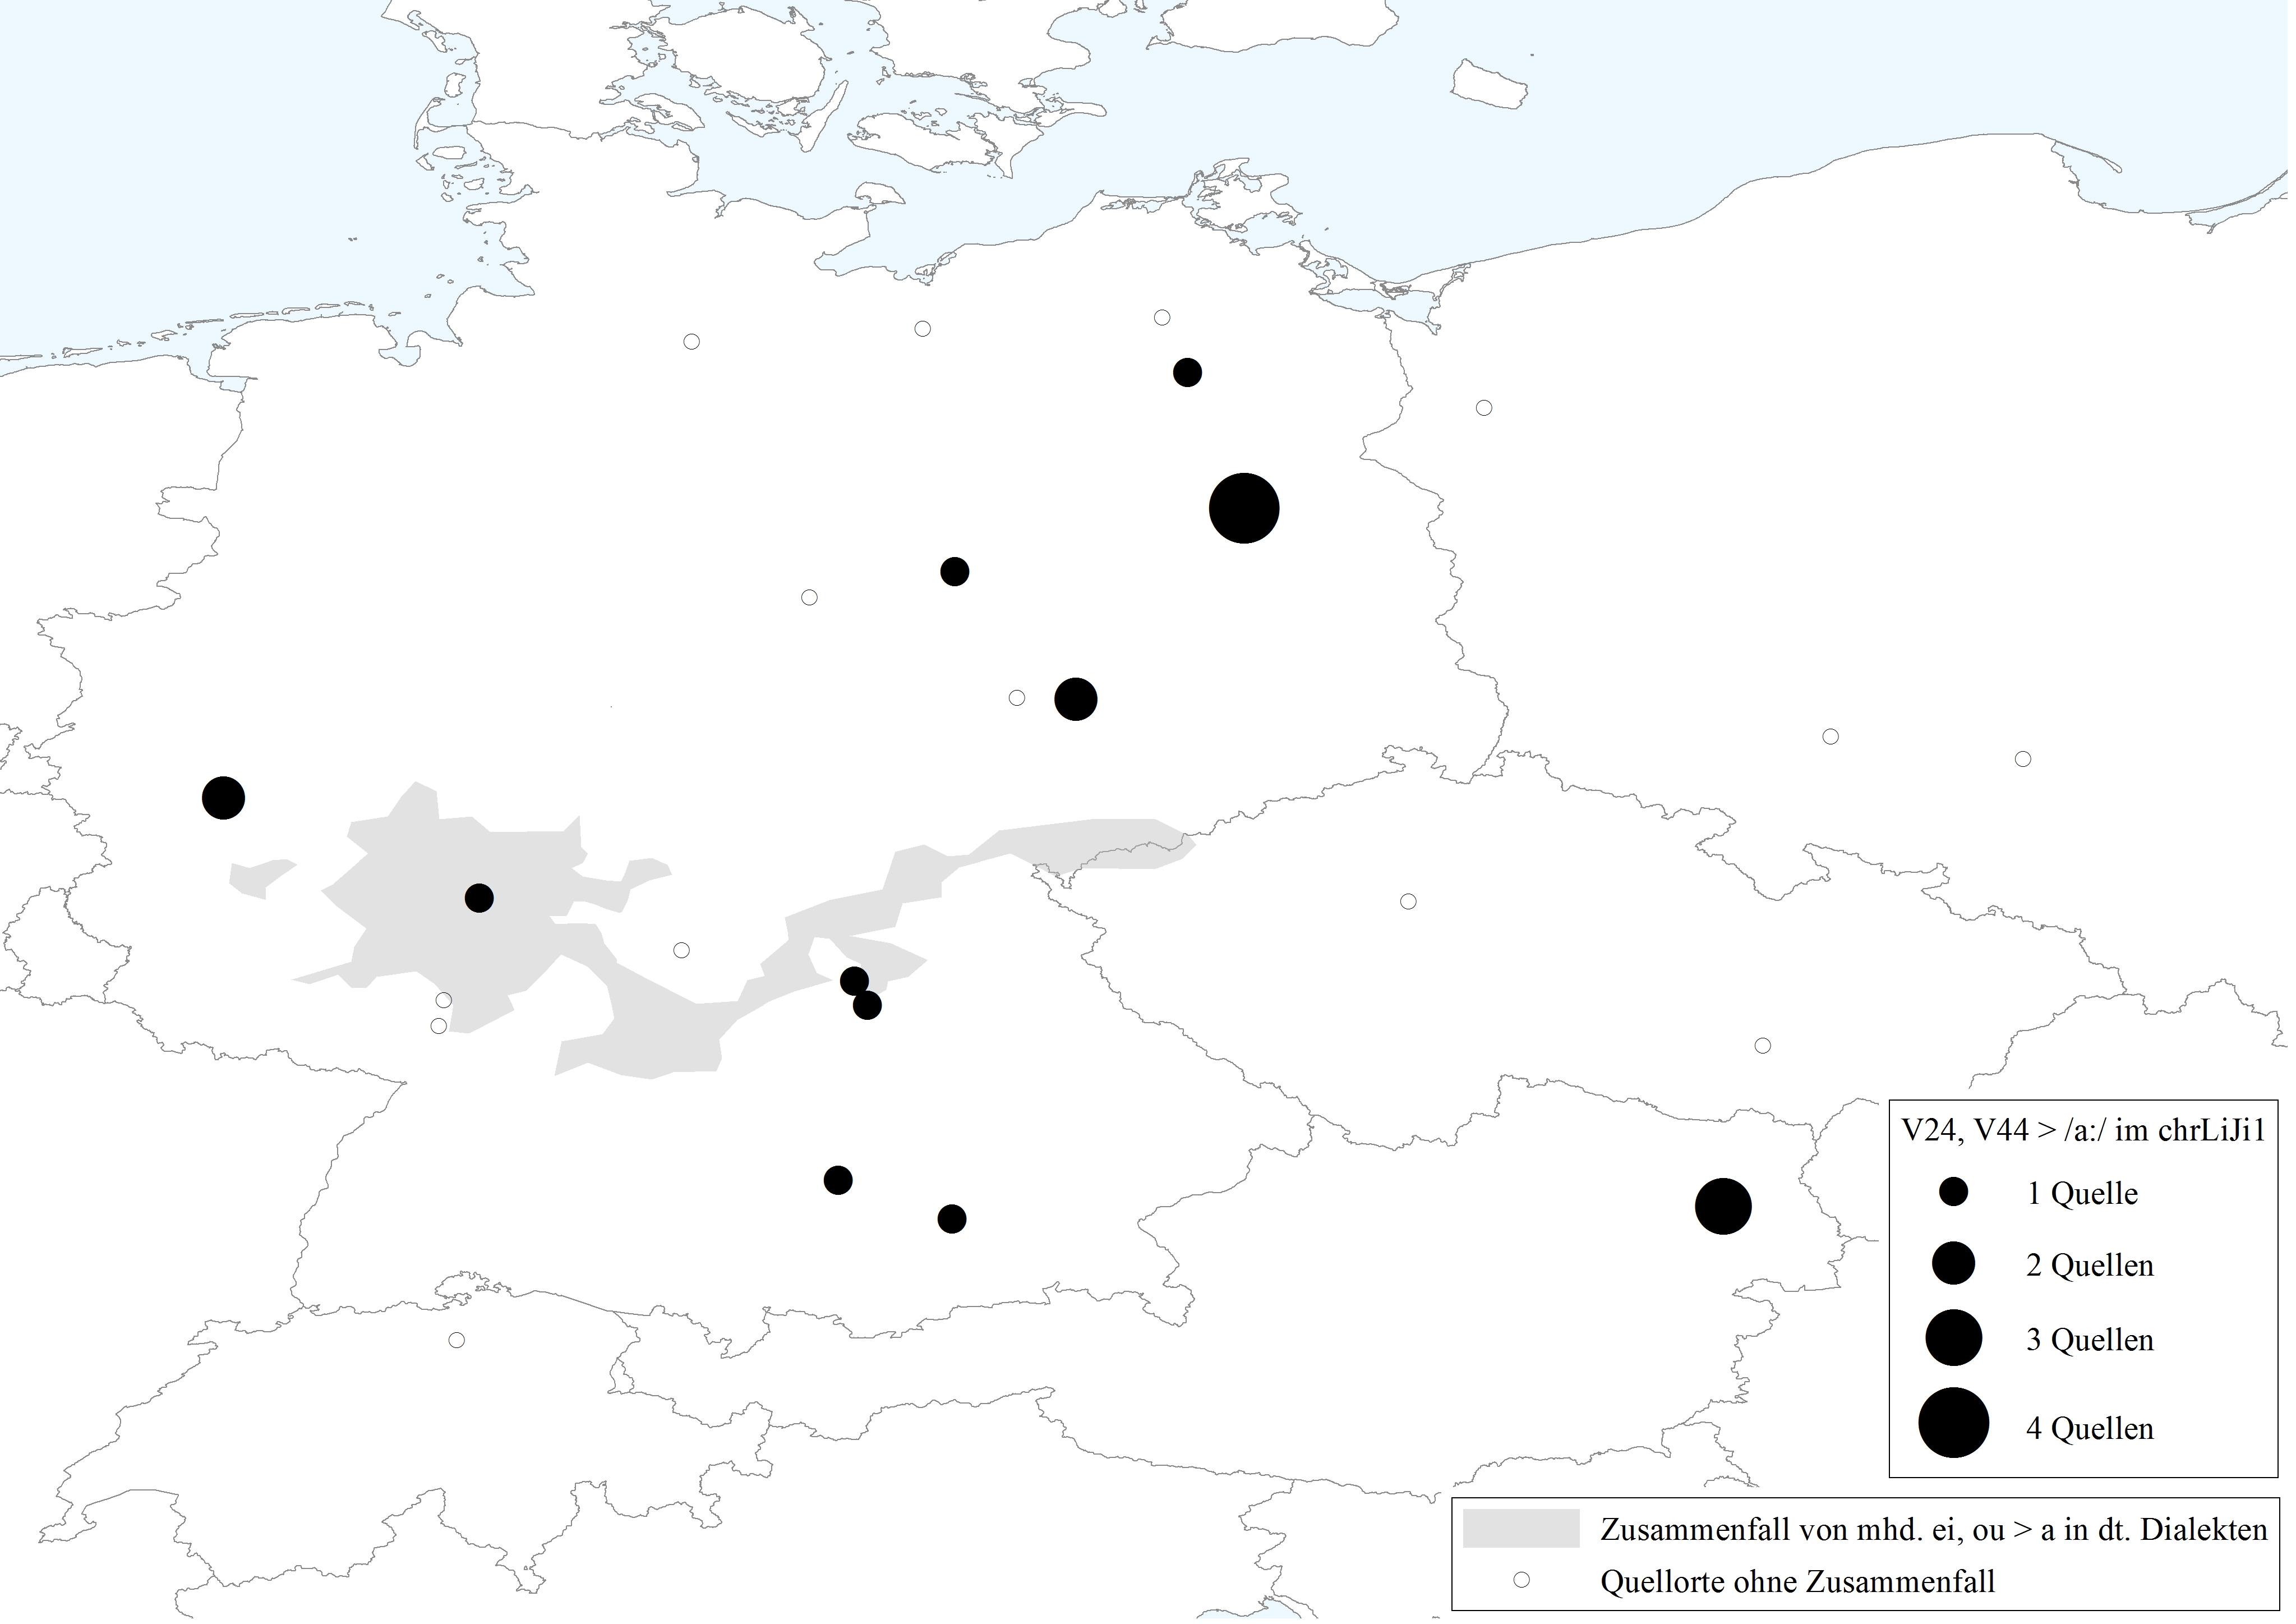
\includegraphics[scale=0.1]{figures/zusammenfallkarte.png}
		\caption{\label{karteV24V44}  Der \isi{Zusammenfall} von \hai{V24} u. \hai{V44} > /a\textlengthmark/ im \hai{chrLiJi1}}
		\end{figure}
\FloatBarrier
 
Sechs von zehn Quellen des \hai{jüdLiJi1} zeigen den \isi{Zusammenfall} (s. Tabelle \ref{tblV24V44}). Anders als im Fall des \hai{chrLiJi1}, sind abweichende Parallelstrategien, wie z.\,B. die Monophthongierung von \hai{V24} zu /e\textlengthmark/ neben der zu /a\textlengthmark/, deutlich seltener.\footnote{Welche Quellen neben dem westjiddischen Monophthong welche Markierungen an der Position von \hai{V24} haben, wird in Tabelle \ref{tblV24uedliji} aufgeführt. Im Vergleich zu den Pamphleten tritt der \isi{Zusammenfall} bzw. treten die einzelnen Monophthongierungen insgesamt in den \hai{GuS} deutlich seltener auf. Eine der Quellen, \hai{GuS15}, zeigt sogar weder die Monophthongierung von \hai{V24} noch die von \hai{V44}.}\\ %Im Fall der Manipulation von \hai{V44} weist nur \hai{PDebrecen} eine Markierung als <o>, <oo>, neben der zu <a> auf.} \hai{jüdLiJi1} ist damit deutlich homogener in seinen Markierungen, was auf eine bessere Sprachkompetenz schließen lässt.\\
 
  \begin{table}[h!]
\centering
		\begin{tabular}{lcc}
		\hline
	\textbf{Quelle} & \textbf{\hai{V24}  > /a\textlengthmark/ }&\textbf{\hai{V44}  > /a\textlengthmark/ } \\ \hline % horizontale Trennlinie
\hai{GuS1}	&  \checkmark&	\checkmark	\\
\hai{GuS5}	&	\checkmark &	–	\\
\hai{GuS10}	&\checkmark&	–\\
 \hai{GuS15} &	–	& –\\	
\hai{GuS23}	&\checkmark&	\checkmark\\
\hai{PAlsleben}	&	\checkmark&		\checkmark\\
\hai{PBerlin1}	&\checkmark&	–\\
\hai{PBerlin2}	&	\checkmark	&\checkmark \\
\hai{PBreslau}	&\checkmark&\checkmark\\	
\hai{PDebrecen}&	\checkmark&\checkmark	\\	\hline
  \end{tabular} 
		 \caption{\hai{V24} und \hai{V44} > /a\textlengthmark/ im \hai{JüdLiJi1}}
		 \label{tblV24V44}
		 \end{table}   
   

 Abschließend lässt sich feststellen, dass die westjiddischen Monophthongierungen von \hai{V24} und \hai{V44} besonders häufig im \hai{LiJi1} auftreten. Eine Nähe zur tatsächlich gesprochenen Sprache ist demnach im \hai{LiJi1} im gesamten 19. Jahrhundert festzustellen. Der für das \hai{WJ} charakteristische \isi{Zusammenfall} von \hai{V24} und \hai{V44} hingegen wird in nur wenigen Quellen vollzogen. Doch immerhin 30\% (16 Texte) des \hai{chrLiJi1}-\isi{Korpus} weisen diesen auf. Diese Quellen geben damit den westjiddischen \isi{Zusammenfall} von mhd. \textit{ei} und \textit{ou} wieder.\\ 
 
 \FloatBarrier
 
 
   \section{\hai{V42} (O\textsubscript{2} = mhd. \textit{ô}) }\label{phonV42}
 %  %\noindent
   
   Eine ebenfalls für das \hai{WJ} typische Entwicklung ist die Diphthongierung von \hai{V42} (mhd.  \textit{ô}) > /\textopeno \textsubarch{u}/ bzw. /a\textsubarch{u}/ (u.\,a. \cite[167]{Timm1987}; \cite[79]{Herzog1992}; \cite[28]{Beider2010}; s. Bsp. \ref{bspV42_1}–\ref{bspV42_4}). \textcite[58f]{GuggenheimGruenberg1973} kartiert für das westl. \hai{SWJ} ausschließlich die Diphthongierung zu /\textopeno \textsubarch{u}/; doch im Elsässer \hai{SWJ} lässt sich auch /a\textsubarch{u}/ finden, wie z.\,B. \ref{bspV42_3}. Die Karte Nr. 30 des \hai{LCAAJ} (\citeyear[79]{Herzog1992}) gibt jedoch zur konkreten  Situation der geographischen Verbreitung dieses Phänomens im \hai{WJ} und in den Übergangsgebieten Rätsel auf: Der Karte zufolge war /\textopeno \textsubarch{u}/ im westjiddischen Gebiet weit verbreitet, während /a\textsubarch{u}/ lediglich an einzelnen Orten des westlichen \hai{WJ},\hai{NÜJ} und \hai{SÜJ} auftrat. An der Karte problematisch ist die quantitative Unausgewogenheit zwischen Flächen (Leitform) und Punkten (singuläre Belege). Zumal angesichts der wenigen Erhebungsorte im \hai{WJ} die Flächenkartierung nicht überinterpretiert werden sollte. Bei genauerer Betrachtung stellt sich heraus, dass /a\textsubarch{u}/  die im westjiddischen Areal weiter verbreitete Variante von \hai{V42} ist und /\textopeno \textsubarch{u}/ hingegen überwiegend in den westjiddischen Varietäten im bairischen, fränkischen, ostfälischen und nordniedersächsischen Raum anzutreffen. Besonders interessant an der Entwicklung von \hai{V42} ist die relativ weit ins \hai{WJ} hineinreichende Form des ostjiddischen Diphthongs /\textopeno \textsubarch{\textsci}/, der laut \hai{LCAAJ} (\citeyear[79]{Herzog1992}) im Jiddischen Berlins, Böhmens und Wiens verbreitet war. \\    
   
       \eenumsentence{\label{bsp42WJ}
    
 % \item östl. \hai{NWJ}:  \textit{Aufen} \sem{Ofen}  < mhd. \textit{oven} \parencite[Bd. 2, Sp. 194]{Lexer1992}\\(Heymann 1909:\,94)   \label{bspV42_1}
   
    \item westl. \hai{NWJ}:  \textit{graus} \sem{groß} 
    < mhd. \textit{grôʒ} \parencite[Bd. 1, Sp. 1093]{Lexer1992}  \\
    (\qu{Das verfrühte Schulenrufen} Aurich 1902:\,3. Auftritt [\cite[132]{Reershemius2007}])   \label{bspV42_1}
    
      \item östl. \hai{NWJ}:  \textit{grauße} \sem{große} 
      \\(Heymann 1909:\,35)   \label{bspV42_1b}
            
    \item \hai{ZWJ}: \RL{גרויזע} \textit{grauze}/\textit{grouze} \sem{große} \\
     (\qu{Die Hochzeit zu Grobsdorf} 1822:\,13)\footnote{Aus dem \hai{ZWJ} sind uns bislang nur authentische Quellen in hebräischen Lettern überliefert. Diese haben den Nachteil, dass man zwar erkennen kann, dass als <\RL{וי}> in der Position von mhd. \textit{ô} ein Diphthong steht, jedoch ist es unmöglich zu bestimmen, auf welchen Diphthong genau dieses Digraph verweist. Die Quellen des \hai{LiJi} können hier Daten liefern, die die Quellen jüdischer Autoren bislang nicht bieten können.} \label{bspV42_2}
    
    \item \hai{SWJ}: \textit{grause} \sem{große} \\
    (\qu{S'frömeläs Etziglä} Colmar 1902:\,5) \label{bspV42_3}
    
    \item oj.: \RL{גרויס} \textit{groys} \label{bspV42_4}    
    }
   
 In den deutschen Dialekten gestaltet sich die Verteilung von aus mhd. \textit{ô} hervorgegangenen Diphthongen  /\textopeno \textsubarch{u}/, /a\textsubarch{u}/ und  /\textopeno \textsubarch{\textsci}/ folgendermaßen (s.\,a. Karte in Abbildung \ref{karteV42}): /\textopeno \textsubarch{\textsci}/ findet sich nach den Karten des \hai{WA} in keinem großflächigen  Areal (\hai{WA} Karten Nr. 419, 219, 411, 159, 382, 351, 192). Im südlichen Rheinfränkisch, im Oberfränkischen und Nordbairischen und einem kleinen Gebiet um Saarbrücken ist /\textopeno \textsubarch{u}/ verbreitet (\hai{WA} Karten Nr. 419, 219, 411, 159, 382, 192;  \cite[237]{Schirmunski1962}). In einzelnen Lexemen, wie etwa \sem{groß} u. \sem{tot}, reicht dieses Gebiet bis ins Mittelbairische hinein (\hai{WA} Karten Nr. 219, 192). Mhd. \textit{ô} > /a\textsubarch{u}/ ist in drei größeren Arealen im Schwäbischen, Westfälischen, Schlesischen und einem kleinen Übergangsgebiet zwischen Brandenburgisch und Ostfälisch vorzufinden (\hai{WA} Karten Nr. 419, 219, 411, 159, 382, 351, 192). Ganz anders, als die westjiddischen Entwicklungen aus \hai{V24} und \hai{V44} haben die westjiddischen Diphthonge aus \hai{V42} ihre Entsprechungen in den deutschen Mundarten nun nicht im Mitteldeutschen, sondern im Ober- und Niederdeutschen. Die Situation in den deutschen Dialekten Österreichs, Liechtensteins und der Schweiz, die die Karten des \hai{WA} nicht erfassen, gestaltet sich nach der Karte Nr. 364 des \hai{KDSA} überwiegend so, dass mhd. \textit{ô} hier überwiegend erhalten blieb; nur im Südbairischen Kärntens und Tirols tritt verbreitet der Diphthong /\textopeno \textsubarch{a}/ auf.

Eine Manipulation von \hai{V42} findet sich im \isi{Korpus} des \hai{chrLiJi1} in 33 Quelltexten. Von diesen verwenden 24 Texte Graphien, die auf den Diphthong /a\textsubarch{u}/ <au> verweisen und acht, welche <ou>, die Leitform des \hai{LCAAJ} (\cite[79]{Herzog1992}), verwenden. In drei dieser acht Quellen wird  parallel  aber auch /a\textsubarch{u}/ eingesetzt. In fünf Texten findet sich der ostjiddische Diphthong als <oi>, <eu>.\footnote{Diese Form steht in drei Quellen parallel zu <au> und in einer dieser drei zusätzlich parallel zu <ou>.} Eine Quelle (\hai{DG} Wien, 1858) weist einen Beleg für <ä> an der Position von \hai{V42} auf. Auch an diesem Phänomen zeigt sich, dass \hai{chrLiJi1} in Fällen von Manipulation Formen des \hai{WJ} verwendet und nur sehr wenige unplausible Formen (etwa der Beleg aus \hai{DG} Wien, 1858) anzutreffen sind. 


Das Histogramm (s. Abb. \ref{V42}) zeigt, dass die Verteilung für \hai{V42} als <au> vorwiegend die früheren Quellen bis etwa 1830 dominiert; später tritt es nur mehr vereinzelt auf. \hai{V42} als <ou> und <oi>, <eu> ist auffällig häufig in Quellen zwischen 1835 und 1845 zu finden. Doch die Belege für <ou> ergeben nicht nur in der diachronen Ansicht ein interessantes Bild, sondern clustern auch stark im Raum (vgl. Abb. \ref{karteV42}).\\

 
  %%%V42Diagramm%\begin{flushleft}	
\begin{figure}[h!]
	\begin{tikzpicture}
		\begin{axis}[only marks, width=0.82\textwidth,height=0.2\textheight,
		legend style={at={(1,1)},xshift=+0.2cm, yshift=0cm,anchor=north west,nodes=left},
			%title={Funktionstypen des sp\"aten Westjiddisch},
			xtick={1700, 1725, 1750, 1775, 1800, 1825, 1850, 1875, 1900, 1925, 1950, 1975}, ytick=\empty,
			x tick label style={/pgf/number format/1000 sep=}, 
			y tick label style={/pgf/number format/1000 sep=},
			%extra y ticks={456.1, 1022.4},
			%extra y tick labels={{456,1},{1022,4}},
			extra y tick style={grid=major,
				tick label style={, ,}},
				ymin=0.7,
				ymax=2.7,
			ylabel={Phänomenbelege},
			enlarge x limits=0.03]	
	
			
\addplot [mark=*, black] table [x=jahr, y=au] {figures/V42au.txt}; %2.3
\addplot [mark=*, gray] table [x=jahr, y=ou] {figures/V42ou.txt}; %2
\addplot [mark=square*, draw=black] table [x=jahr, y=oi] {figures/V42oi.txt}; %1.7
\addplot [mark=triangle*, draw=black] table [x=jahr, y=ae] {figures/V42ae.txt}; %1.4
\addplot [mark=o, black] table [x=jahr, y=no] {figures/V42no.txt}; %1.1

			% Andere Formen a={mark=square*,blue},% b={mark=triangle*,red},% c={mark=o,draw=black}}
						\legend{\hai{V42} als <au>, \hai{V42} als <ou>, \hai{V42}  als <eu>, \hai{V42} als <ä> , unmanipuliert} %macht Legende
		\end{axis}
	\end{tikzpicture}
	\caption{\hai{V42} im \hai{chrLiJi1}}
	\label{V42}	
\end{figure}
\FloatBarrier



Die regionale Verteilung der im \hai{chrLiJi1} vorliegenden Manipulationen von \hai{V42} zeigt ein interessantes Bild (Abbildung \ref{karteV42}). \hai{V42} als <au> streut weiter in das westjiddische und übergangsjiddische Gebiet hinein, als es die Karte des \hai{LCAAJ} \textcite[79]{Herzog1992} angibt. Die Leitform des \hai{LCAAJ},  /\textopeno \textsubarch{u}/ <ou>, hingegen findet sich lediglich in einem Areal koterritorial zum Rheinfränkischen und Mittelbairischen, wo in den deutschen Mundarten dieselbe Entwicklung stattgefunden hat. Es ist nicht zu entscheiden, ob uns hier im \hai{chrLiJi1} korrekte Imitationen des örtlichen \hai{WJ} vorliegen, oder ob es sich bei der \isi{Imitation} um Interferenzen mit dem eigenen deutschen Dialekt handelt. An dieser Stelle stößt die Analyse an ihre Grenzen. Es darf angenommen werden, dass /\textopeno \textsubarch{u}/ <ou> der ältere aus \hai{V42} hervorgegangene Diphthong ist, welcher sich in manchen Teilen des Westjiddischen entweder durch den Kontakt zu den deutschen Dialekten oder unabhängig von ihnen zu /a\textsubarch{u}/ weiter entwickelt hat bzw. im Ostjiddischen zu /\textopeno \textsubarch{u}/ wurde. Bislang ist /\textopeno \textsubarch{u}/ lediglich für südwestjiddische und südliche zentralwestjiddische Varietäten belegt (vgl. \cite[58f]{GuggenheimGruenberg1973}).\footnote{Eine punktgenauere Darstellung der Daten, die die Grundlage der Kartierung des \hai{LCAAJ} (\citeyear[79]{Herzog1992}) waren, würden hier evtl. von Nutzen sein. Für die älteren Quellen, d.\,h. hebräischschriftliche Texte, sehen wir uns mit dem Problem konfrontiert, dass <\RL{וי}> sowohl für den Diphthong <ou>, als auch für <au> stehen kann. In den Editionen zweier in Quadratschrift geschriebener maskilimischer Quellen von \textcite{AptrootGruschka2004} und \textcite{copeland1976} werden <\RL{וי}> als <ou> transliteriert, doch ist gerade die Interpretation dieses Graphems äußerst problematisch, da sie ebenso für /a\textsubarch{u}/ oder  /\textopeno \textsubarch{\textsci}/ verwendet wird  (vgl. \cite[167]{Timm1987}). Hinzu kommt, dass die erste Transliteration von Joseph Herz \quji{\RL{אסתר}} (Fürth 1871) durch J. Suhler (Fürth 1871; Abdruck in Israelische Kultusgemeinde Fürth 1984–1986) <au> für <\RL{וי}> schreibt. Erst eine erneute, sensitivere Kartierung der Daten des \hai{LCAAJ} würde es erlauben zu entscheiden, wie sich die aus \hai{V42} hervorgegangenen Diphthonge im \hai{WJ} Sprachraum verhalten und wie deren Verhältnis zu den deutschen Dialekten genau aussieht.} Was die Belege für \hai{V42} als <eu>, <oi> betrifft, so muss offen bleiben, ob hier das aus dem \hai{OJ} bekannte Merkmal in die \isi{Imitation} einfloss oder ob es möglicherweise tatsächlich vereinzelt gesprochen wurde, was wiederum der Karte des \hai{LCAAJ} (\cite[79]{Herzog1992}) zu Folge nicht auszuschließen ist. \\
 
 
  \begin{figure}[h!]
		\centering
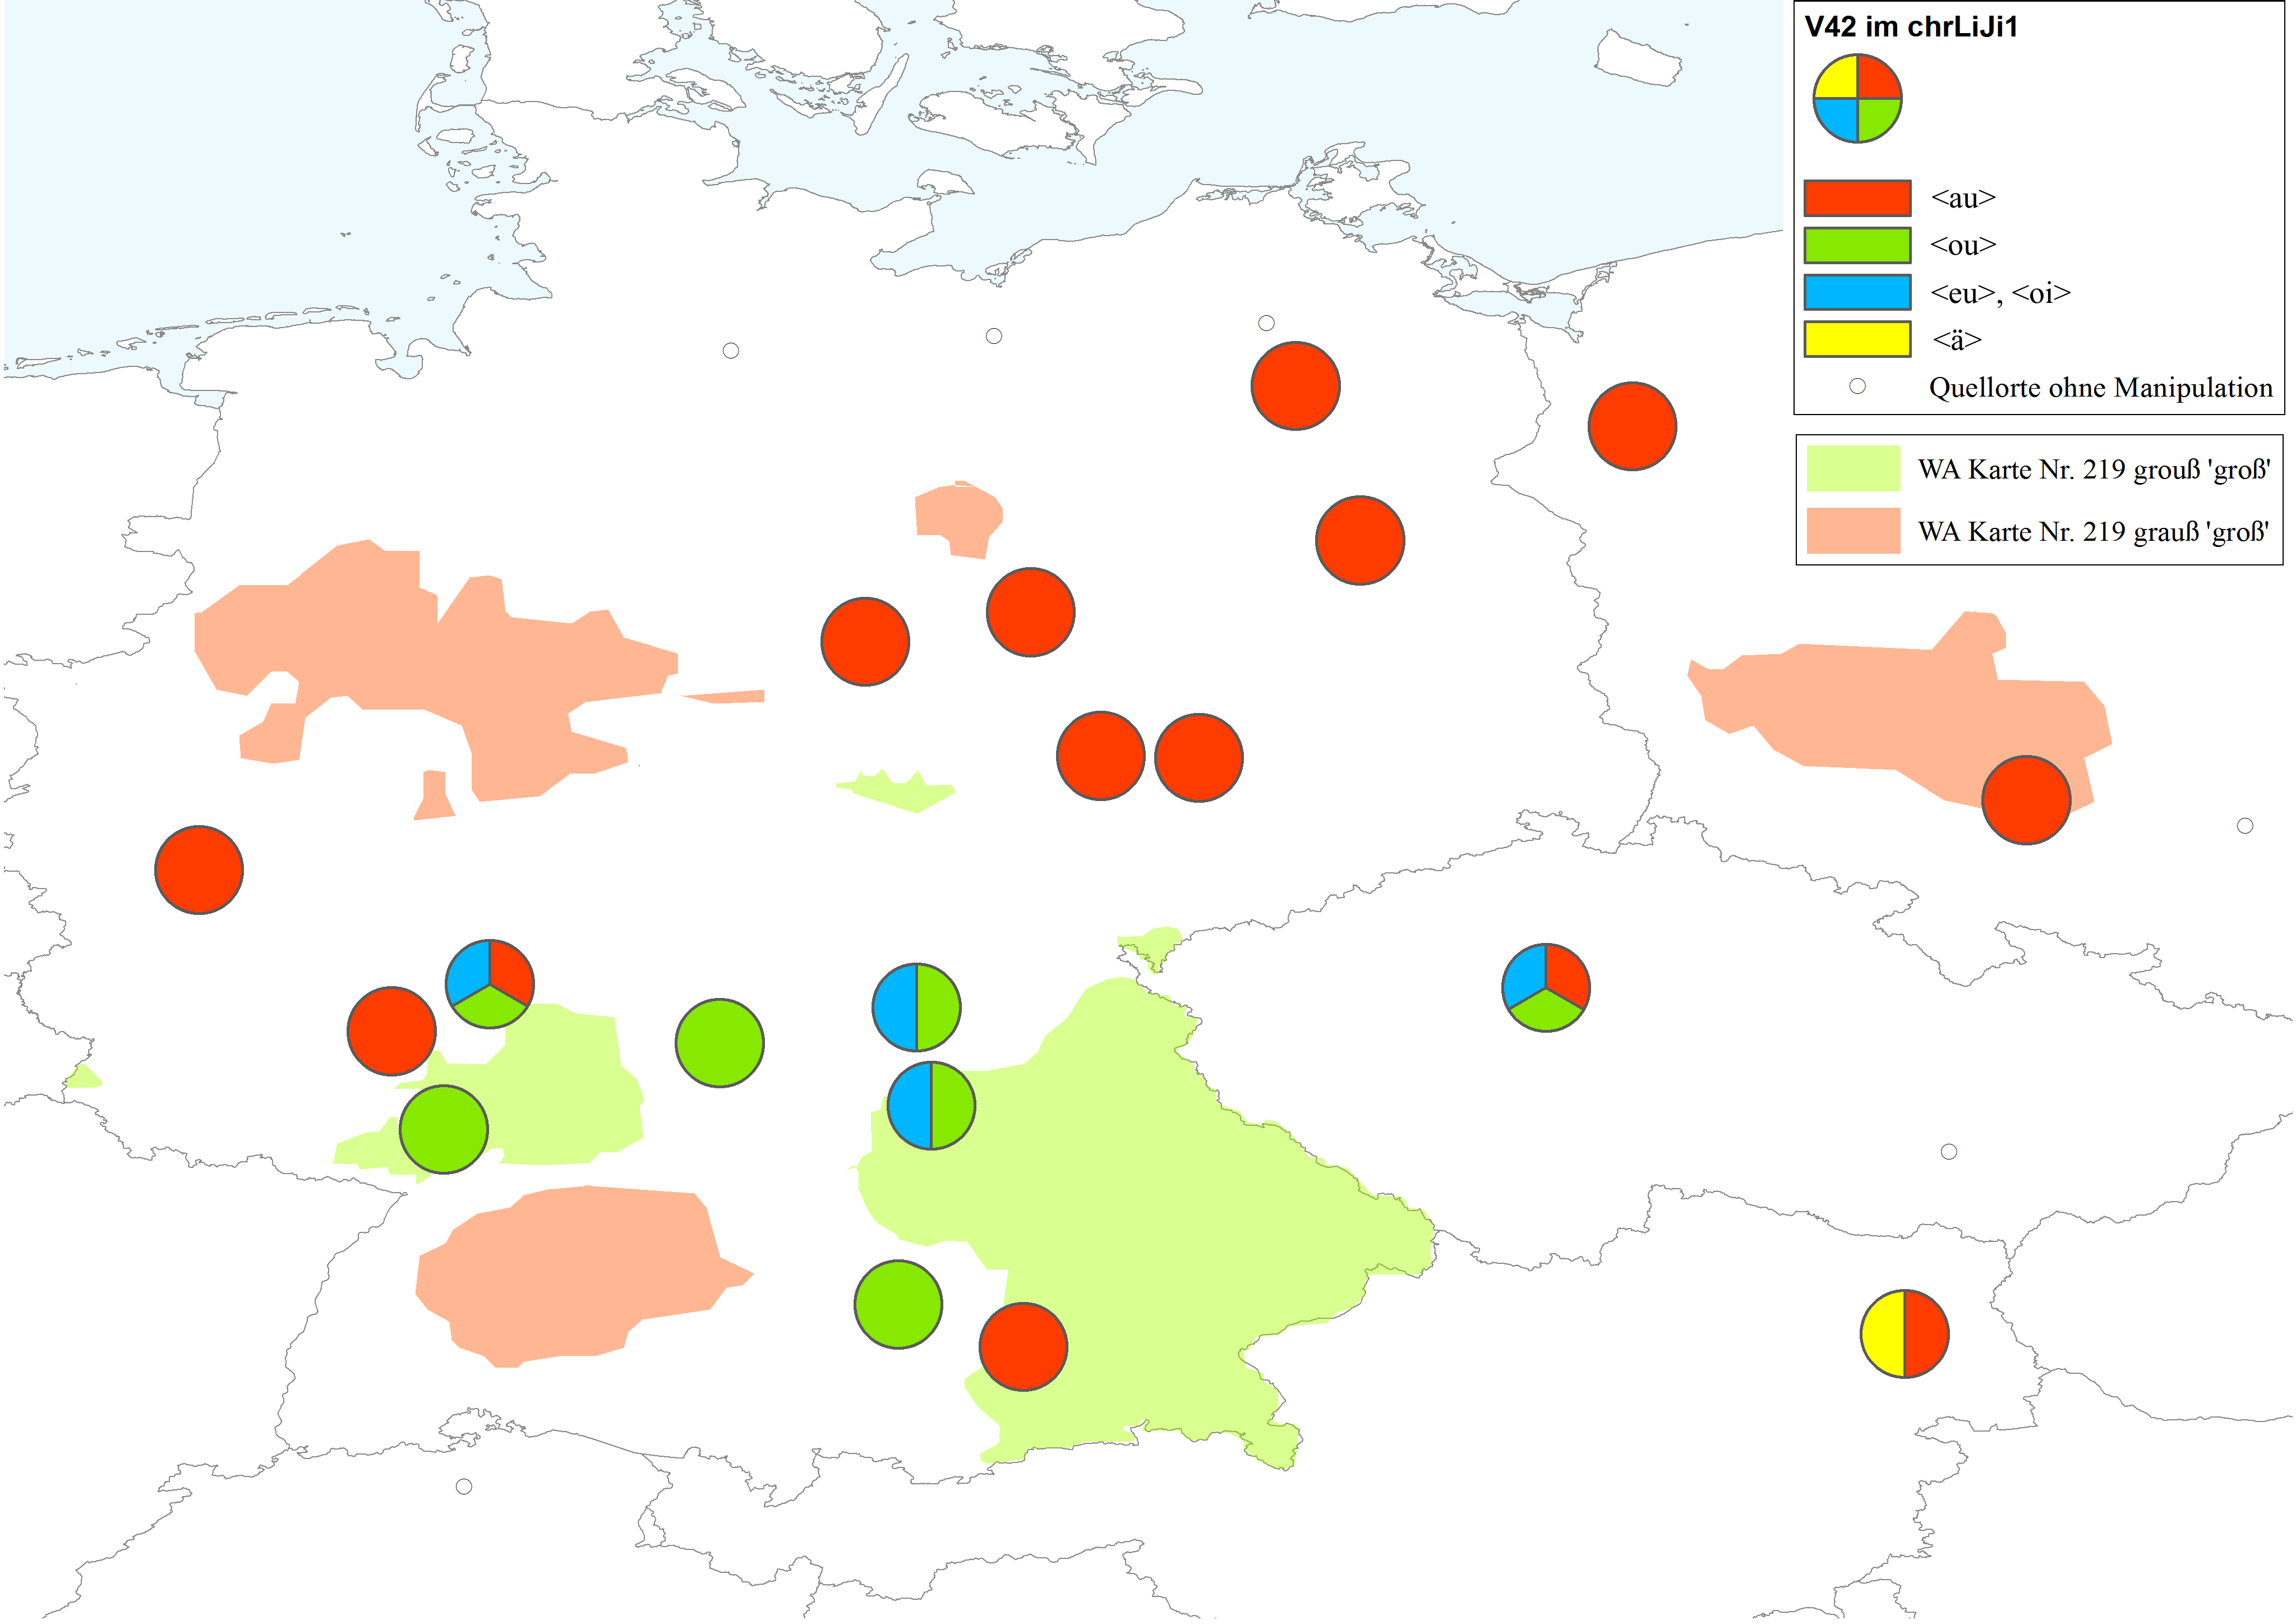
\includegraphics[scale=0.1]{figures/V42allDSA2.png}
		\caption{\label{karteV42}  \hai{V42} im \hai{chrLiJi1} mit \hai{WA} Karte Nr. 219}
		\end{figure}
\FloatBarrier
 


   
   
 In sechs der zehn Quellen des \hai{jüdLiJi1} findet sich eine Manipulation von \hai{V42}. In allen Fällen handelt es sich dabei um die Diphthongierung zu  <au>.\footnote{Die entsprechenden Quellen sind \hai{GuS1}, \hai{GuS5}, \hai{PAlsleben}, \hai{PBerlin1}, \hai{PBerlin2} und \hai{PBreslau}.} In \hai{GuS1} findet sich neben dem westjiddischen Diphthong auch der ostjiddische Diphthong  <oi> belegt. <ou> ist nicht zu finden; allerdings stammt auch keine Quelle aus der relevanten Region. Eine nicht in das \isi{Korpus} aufgenommene Quelle des \hai{jüdLiJi1} aus dem fränkischen Raum wäre Jakob Wassermanns \qu{Die Juden von Zirndorf} (1897). Hier finden sich in einem Lexem der Diphthong <ou> belegt: \textit{Jou} (Wassermann [1897] 1996:\,189, 190) \sem{Ja} < mhd. \textit{jô} / \textit{jû} \parencite[Bd. 1, Sp. 1481]{Lexer1992}.\\
 


Zusammenfassend lässt sich feststellen, dass sich Manipulationen von \hai{V42} in allen drei Korpora sehr homogen gestalten: Wenn diese Position manipuliert wird, dann zu einem Diphthong, der die jeweilige Sprachrealität abbildet. Es liegen kaum unplausible Formen der \isi{Imitation} von \hai{V42} vor. \\ 
 \FloatBarrier

   
 \section{\hai{V22} (E\textsubscript{2} = mhd. \textit{ê}, \textit{œ})}\label{phonV22}
 %\noindent
 In allen jiddischen Mundarten sind mhd. \textit{ê}, \textit{œ} (urj. \textit{*\=e\textlengthmark}) zu einem Diphthong zusammengefallen. Im \hai{WJ}, \hai{SOJ} und \hai{NOJ} erfolgte der \isi{Zusammenfall} zu /ɛ\textsubarch{\textsci}/, im \hai{ZOJ} zu /a\textsubarch{\textsci}/ (u.\,a. \hai{LCAAJ} \textcite[72]{Herzog1992};  \cite{Timm1987}; \cite{Beider2010}; erstmals in Boeschenstein 1592 zit. n. \cite[3]{Mieses1915}; s. Bsp. \ref{bspv22_1}–\ref{bspv22_2}). In den deutschen Dialekten ist dieser \isi{Zusammenfall} von mhd. \textit{ê} und \textit{œ} > \textit{aj} äußerst selten (\hai{WA} Karten Nr. 461, 167; \hai{KDSA} Karten Nr. 378, 382; vgl. Karte in Abb. \ref{karteV22}). Im Binnensprachgebiet ist er lediglich in einem kleinen Gebiet des östlichen Rheinfränkischen anzutreffen; daneben findet man ihn in Grenz- und Siedlungsmundarten des burgenländischen, böhmischen und mährischen Bairischen. Das größte Areal, in dem diese Entwicklung stattgefunden hat, findet sich im Nordschlesischen. Es fällt auf, dass dieser \isi{Zusammenfall} überwiegend in Kontaktgebieten zu slawischen Sprachen und dem Ungarischen stattgefunden hat.\\
 
\eenumsentence{ 
 

\item \RL{גֵיהן} \textit{geyhn} \sem{gehen} \\
 (\qu{Die Hochzeit zu Grobsdorf} 1822:\,33) < mhd. \textit{gên}; oj. \RL{גיין} \textit{geyn} \label{bspv22_1}

\item \RL{ שֵיא} \textit{shey} \sem{schön}\\
 (\qu{Die Hochzeit zu Grobsdorf} 1822:\,19) < mhd. \textit{schœne}; oj. \RL{שיין} \textit{sheyn} \label{bspv22_2}

 } 
 
  Von allen 36 Quellen des \hai{chrLiJi1}, die eine Manipulation von \hai{V22} zeigen, wird ein  Diphthong in dieser Position als <ai> (20 Texte), <ei> (neun Texte), <ey> (sechs Texte) oder <ay> (ein Text) verwendet. Die Kartierung der Graphien ergab keine räumlichen Muster. Es ist generell fragwürdig, welchen Zweck die besonderen Graphien des Diphthongs erfüllen sollen; scheinbar wurde der Diphthong als vom standarddeutschen /a\textsubarch{\textsci}/ <ei> abweichend dargestellt. Es ist aber auch möglich, dass durch die Graphie als <ai> ein \isi{phonetisch} geeigneteres Graphem des Diphthongs /a\textsubarch{\textsci}/ verwendet wurde, als das im deutschen Standard übliche <ei>, welches eine größere graphem-phonematische Distanz zum tatsächlichen Laut aufweist. Die unterschiedliche Schreibweise in \qu{Die Hochzeit zu Grobsdorf} der Vokale \hai{V22} (als <\RL{י}\RL{ֵ} >, s. Bsp.  \ref{bspv22_1}–\ref{bspv22_2}, S. \pageref{bspv22_1}) und \hai{V34}  (als <\RL{יי}> , s. Bsp. \ref{grobbspv34_1}–\ref{grobbspV34_2}, S. \pageref{grobbspV34_2}) spricht allerdings stark dafür, eine unterschiedliche Aussprache der beiden Vokale auch im Westjiddischen anzunehmen. Da aber im Fall des \hai{LiJi} nicht zu entscheiden ist, welcher Laut sich tatsächlich hinter welchem Graphem verbergen soll (und tatsächlich auch nicht, wie <ei> im 19. Jahrhundert von Sprechern des Deutschen realisiert wurde), wird im folgenden /ɛ\textsubarch{\textsci}/ als der im \hai{WJ} gebräuchliche Diphthong idealisierend gesetzt. 
 
Für die Graphie interessant sind die Belege aus den beiden kleineren Korpora: Im \hai{jüdLiJi1} zeigen acht der zehn Quellen eine Manipulation von \hai{V22} als <ei>.\footnote{Dies betrifft die Texte \hai{GuS1,5,15,23}, \hai{PAlsleben}, \hai{PBerlin1}, \hai{PBerlin2} und \hai{PBreslau}. Die Texte \hai{GuS23}, \hai{PAlsleben} u. \hai{PBerlin2} zeigen nur Belege für den Diphthong < mhd.  \textit{ê}. Die  übrigen fünf Quellen haben den \isi{Zusammenfall} belegt.} Alle dieser Texte setzen <ei>, also das standarddeutsche Graphem. 


Es lässt sich festhalten, dass die orthographischen Strategien im \hai{jüdLiJi1} insgesamt näher am gesprochenen Laut /ɛ\textsubarch{\textsci}/ sind als die des \hai{chrLiJi1}.
 
 Die Hauptbelege einer Manipulation von \hai{V22} in allen Korpora treten  am Kennlexem \sem{wehe} auf (vgl. Unterabschnitt \ref{interjektionen}), welches die Belegzahlen zu diesem Phänomen in die Höhe treibt. Der \isi{Zusammenfall} selbst ist im \hai{chrLiJi1} nur in neun Texten belegt,\footnote{Die entsprechenden Quellen sind \hai{AD} (Leipzig, 1846), \hai{AJ} (Berlin, 1825), \hai{AK} (Zürich, 1948), \hai{DW} (Wien, 1773), \hai{MV} (Berlin, 1862), \hai{NW} (Berlin, 1804), \hai{SV} (München, 1890), \hai{TH} (Merseburg, 1820) u. \hai{VD} (Frankfurt, 1916).} eine Quelle manipuliert nur mhd. \textit{œ},\footnote{Es handelt sich um die Quelle \hai{WA} (Magdeburg, 1802).} die übrigen 23 Quellen manipulieren lediglich mhd. \textit{ê}.  Das Histogramm in Abbildung \ref{V22zusammen} zeigt, dass der \isi{Zusammenfall} v.\,a. in Quellen des frühen 19. Jahrhunderts zu finden ist, aber auch in den späteren Quellen  auftaucht.\\

  %%%V22Diagramm%\begin{flushleft}	
\begin{figure}[h!]
	\begin{tikzpicture}
		\begin{axis}[only marks, width=0.82\textwidth,height=0.2\textheight,
		legend style={at={(1,1)},xshift=+0.2cm, yshift=-0.44cm,anchor=north west,nodes=left},
			%title={Funktionstypen des sp\"aten Westjiddisch},
			xtick={1700, 1725, 1750, 1775, 1800, 1825, 1850, 1875, 1900, 1925, 1950, 1975}, ytick=\empty,
			x tick label style={/pgf/number format/1000 sep=}, 
			y tick label style={/pgf/number format/1000 sep=},
			%extra y ticks={456.1, 1022.4},
			%extra y tick labels={{456,1},{1022,4}},
			extra y tick style={grid=major,
				tick label style={, ,}},
				ymin=0.7,
				ymax=2.7,
			ylabel={Phänomenbelege},
			enlarge x limits=0.03]	
	
			
\addplot [mark=*, black] table [x=jahr, y=zusammenfall] {figures/V22zusammenfall.txt}; %2.1
\addplot [mark=*, gray] table [x=jahr, y=nur_e] {figures/V22nur_e.txt}; %1.7
\addplot [mark=square*, draw=black]  table [x=jahr, y=nur_oe] {figures/V22nur_oe.txt}; %1.3
\addplot [mark=o, black] table [x=jahr, y=no] {figures/V22no2.txt}; %1.1


 

			% Andere Formen a={mark=square*,blue},% b={mark=triangle*,red},% c={mark=o,draw=black}}
						\legend{mhd. \textit{ê}, \textit{œ} als <ei>, mhd. \textit{ê} als <ei>,  mhd. \textit{œ} als <ei>,  unmanipuliert} %macht Legende
		\end{axis}
	\end{tikzpicture}
	\caption{Der \isi{Zusammenfall} von \hai{V22} im \hai{chrLiJi1}}
	\label{V22zusammen}	
\end{figure}
\FloatBarrier
 
 
 Die räumliche Verteilung zeigt, dass bei diesem Phänomen keine Beeinflussung durch deutsche Dialekte im \hai{chrLiJi1} vorliegt (Karte in Abb. \ref{karteV22}). Die Regionen, in denen der \isi{Zusammenfall} von mhd. \textit{ê}, \textit{œ} > /ɛ\textsubarch{\textsci}/ in den deutschen Dialekten stattfand, sind im Projektsample des \hai{chrLiJi1} kaum vertreten. Einzige Ausnahme bildet Wien, wo der \isi{Zusammenfall} sowohl im \isi{Korpus} als auch in der näheren Umgebung im deutschen Dialekt gegeben ist. Durchaus interessant sind die Raumbilder der Karte \ref{karteV22} dennoch. Allem Anschein nach sind Diphthongierungen, die zu einem \isi{Zusammenfall} von mhd. \textit{ê}, \textit{œ} > /ɛ\textsubarch{\textsci}/ führen, auch in den deutschen Mundarten deutlich aneinander gebunden. Die Diphthongierung von mhd.\textit{œ} findet selten ohne die von mhd. \textit{ê} statt (und umgekehrt), was darauf schließen lässt, dass der \isi{Zusammenfall} nicht auf direktem Weg durch die Diphthongierung erfolgte, sondern die \isi{Entrundung} von \textit{œ} > \textit{ê}  bereits zum \isi{Zusammenfall} mit mhd. \textit{ê} geführt hat. Wie auch im \isi{Zusammenfall} von mhd. \textit{ei} und \textit{ou} > /a\textlengthmark/ (Abb. \ref{dteiou}) entsprechen (west-)jiddische Entwicklungen damit Strukturen, wie sie auch in den deutschen Dialekten vorherrschen. \\ 
 
 
  \begin{figure}[h!]
		\centering
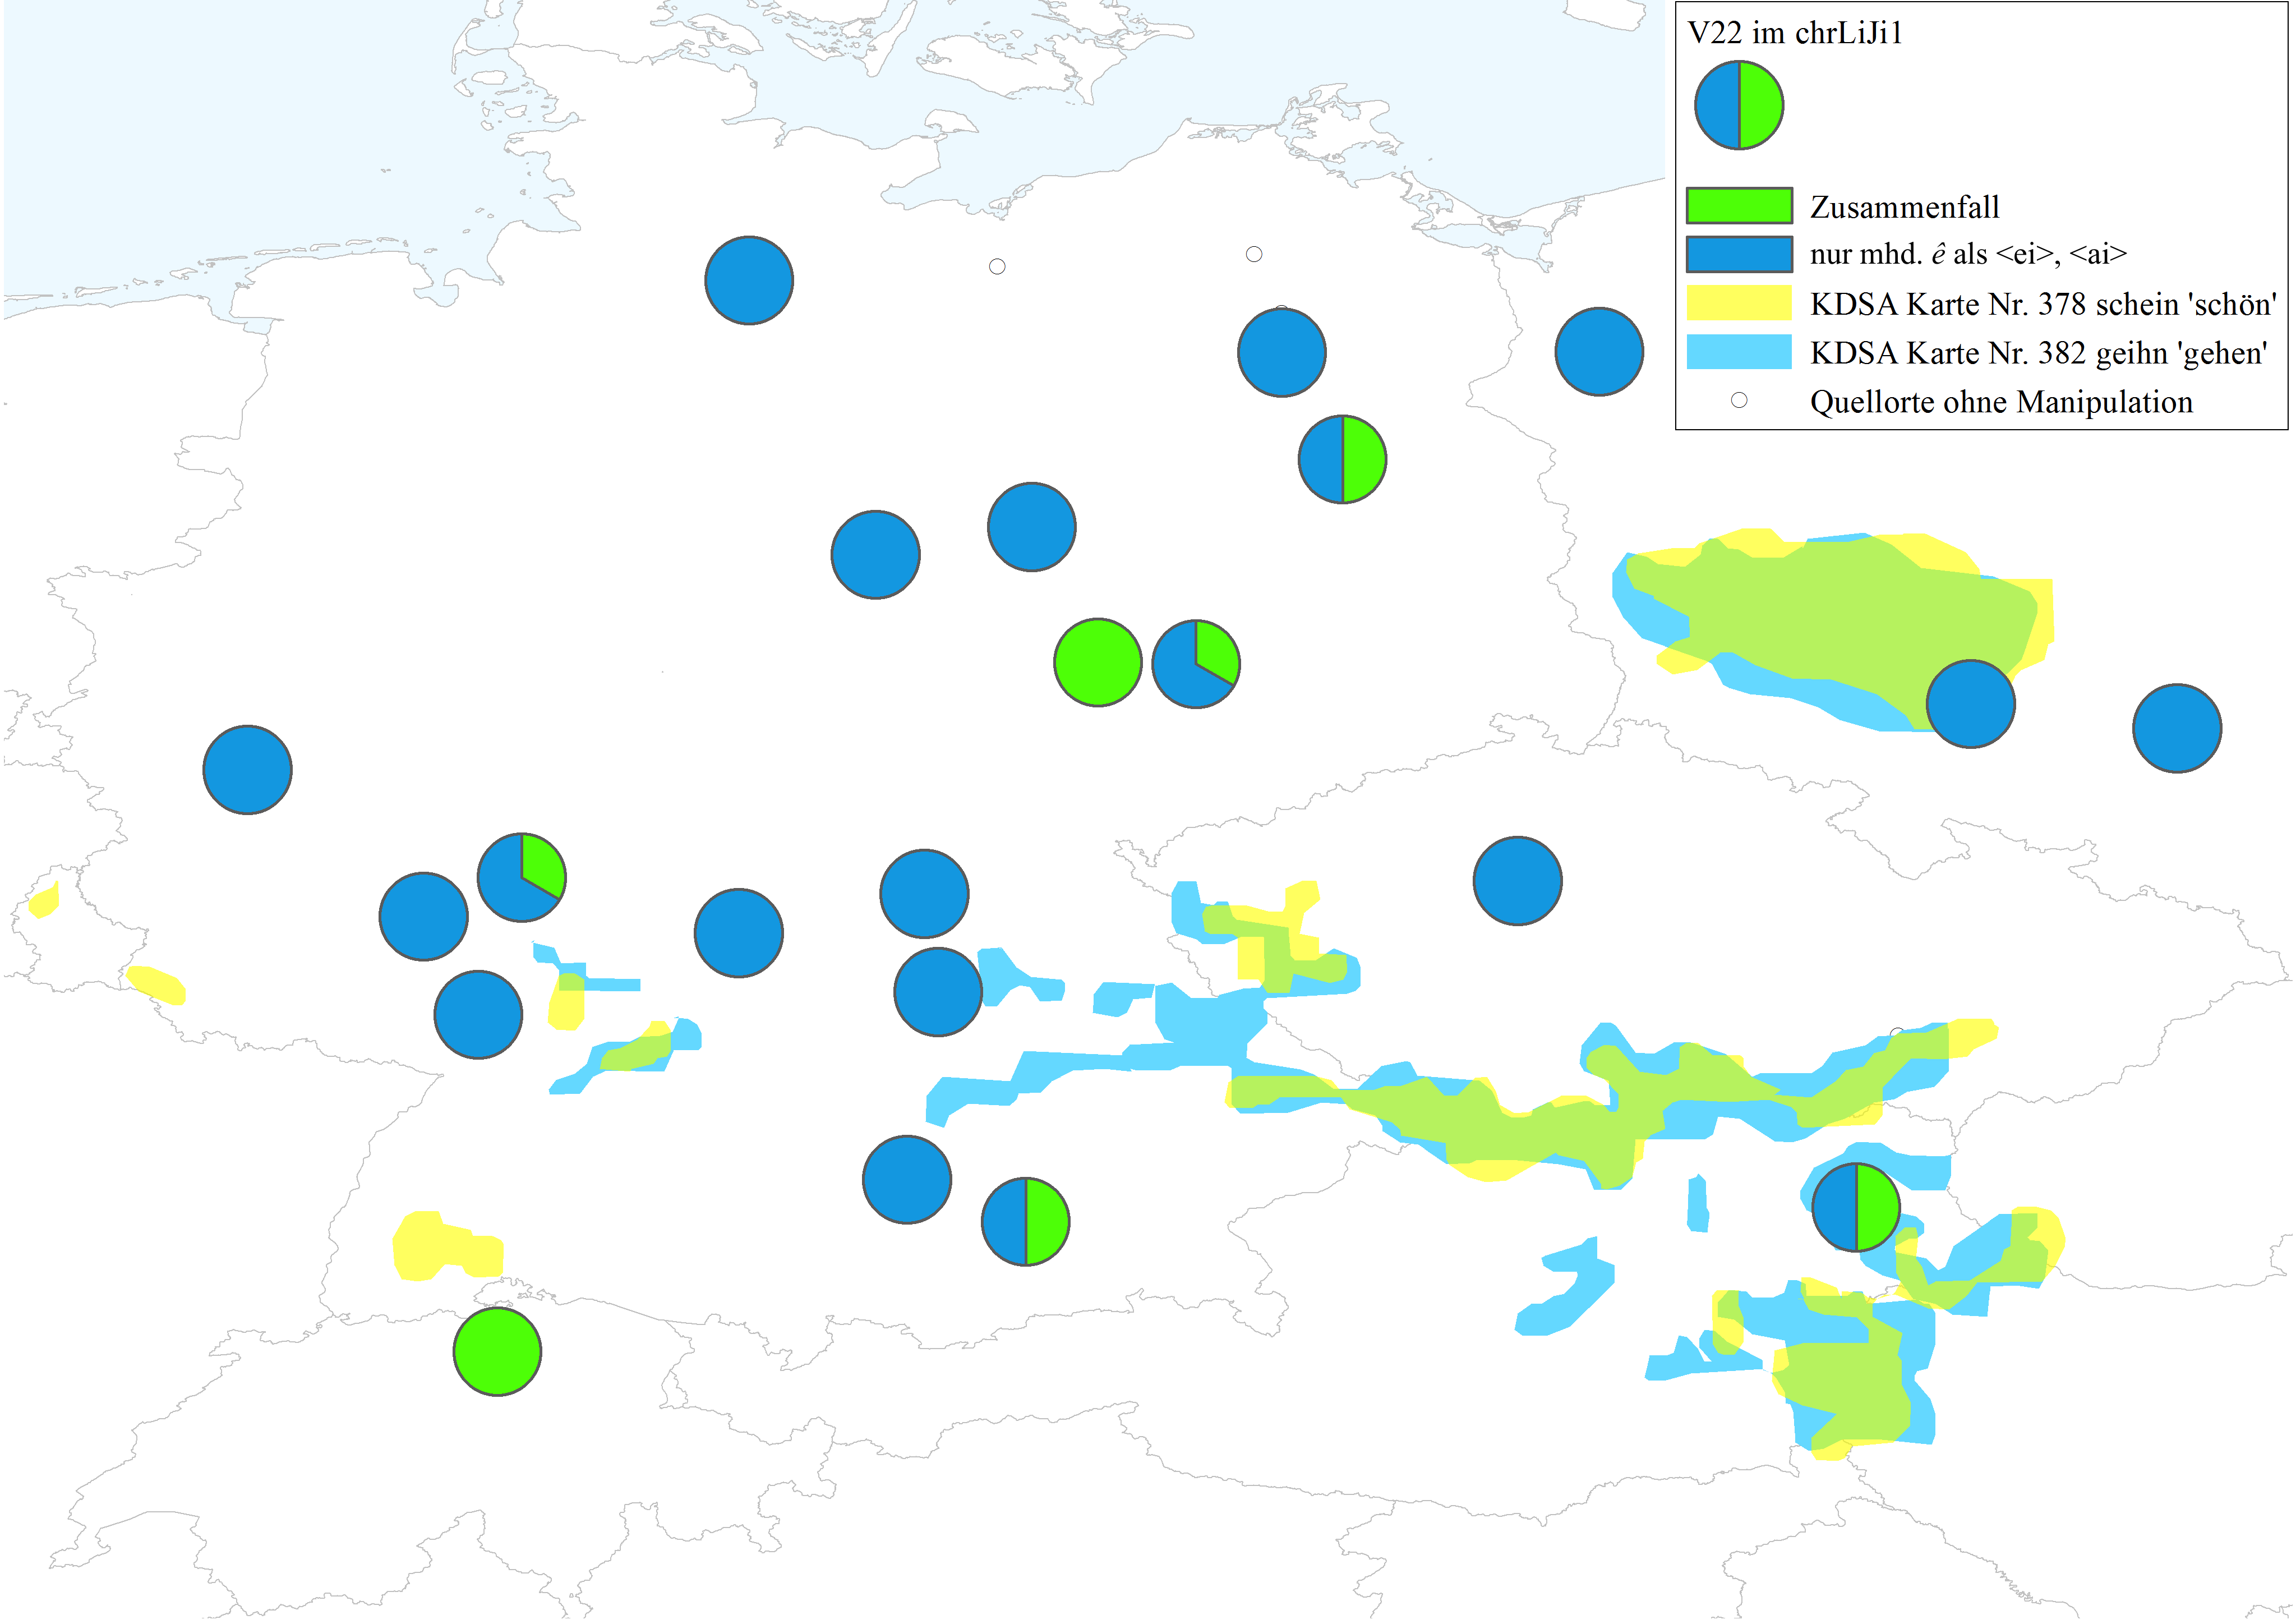
\includegraphics[scale=0.1]{figures/V22zusammenfall2.png}
		\caption{\label{karteV22}  \hai{V22} im \hai{chrLiJi1} mit \hai{KDSA} Karten Nr. 378, 382}
		\end{figure}
\FloatBarrier
 



 
 
 \section{\hai{V34} (I\textsubscript{4} = mhd. \textit{iu}, \textit{î})}\label{phonV35}

Mhd. \textit{iu} und \textit{î} sind in den meisten west- und ostjiddischen Dialekten zu /a\textsubarch{\textsci}/ zusammengefallen (\hai{LCAAJ} \cite[77]{Herzog1992}; \cite[206]{Timm1987}; s. Bsp. \ref{grobbspv34_1}--\ref{grobbspv34_2}, s.\,a. Bsp. \ref{bspV34_1}–\ref{bspV34_4} S. \pageref{bspV34_1}). Im \hai{ZOJ}, östlichen \hai{SÜJ} und südlichen \hai{SOJ} ist dieser Diphthong zu /a\textlengthmark/, bzw. /a/ im \hai{SOJ} monophthongiert worden (\cite[77]{Herzog1992};\cite[206]{Timm1987}; s. Unterabschnitt \ref{hyperV24}). Den westjiddischen Diphthong /a\textsubarch{\textsci}/ < mhd. \textit{iu} findet man in den deutschen Dialekten sehr weit verbreitet. Er deckt besonders große Teile des östlichen Sprachgebiets ab (\hai{WA} Karten Nr. 319, 463, 497, 519, 542; \hai{KDSA} Karte Nr. 410). Eine Entwicklung von mhd.  \textit{iu} > /a\textsubarch{\textsci}/ ist in den oberdeutschen Dialekten keine Seltenheit. Dort ist der Diphthong, mit Ausnahme des Alemannischen,\footnote{Schwäbisch, was hier nicht im eigentlichen Sinn als Alemannisch verstanden wird, da es u.\,a. die sog. \quein{nhd. Diphthongierung u. Monophthongierung} mitgemacht hat, zeigt ebenfalls mhd.  \textit{iu} > /a\textsubarch{\textsci}/.} in großen Teilen des Ostmittel- und Ostniederdeutschen, sowie im Rhein-, Mosel- und Niederfränkischen und in nordniederdeutschen Übergangsgebieten belegt (vgl.\hai{WA} Karten Nr. 463, 519, 196). \\



\eenumsentence{
 

\item \RL{נייא} \textit{ney} \sem{neu} 
(\qu{Die Hochzeit zu Grobsdorf} 1822:\,21) 
\\ < mhd. \textit{niuwe}; vgl. oj. \RL{נ{יי}\makebox(-1.5,-7.5)[r]{\libertineGlyph{uni207B}}} \textit{nay} \label{grobbspv34_1}

\item \RL{בראנטעווייא} \textit{brantwey} \sem{Branntwein}
 (\qu{Die Hochzeit zu Grobsdorf} 1822:\,7) \\
 < mhd. \textit{wî}; vgl. oj. \RL{וו{יי}\makebox(-1.5,-7.5)[r]{\libertineGlyph{uni207B}}ן} \textit{vayn}\label{grobbspv34_2}
 
 }



Die Diphthongierung von mhd. \textit{î} > /a\textsubarch{\textsci}/ haben im Zuge der
\quein{neuhochdeutschen Diphthongierung} zwischen dem 12. und 16. Jahrhundert neben dem Jiddischen alle hochdeutschen Dialekte (mit Ausnahme des Alemannischen) mitgemacht (\cite[146–149]{Koenig1978}; \cite[14–18]{Timm1987}). Dieser Diphthong ging auch in die Leitvarietät über und ist damit Bestandteil des Neuhochdeutschen. Eine Weiterentwicklung von mhd. \textit{î} > /a\textsubarch{\textsci}/, wie z.\,B. die Rückmonophthongierung im \hai{ZOJ}, hat in kaum einem Dialekt stattgefunden (vgl. \hai{WA} Karten Nr. 15, 176, 180). Da die westjiddische Form dem Schriftdeutschen entspricht, kann nicht überprüft werden, ob Belege für <ei>, <ai> an der Position von mhd. \textit{î} in \isi{Analogie} zum Jiddischen gesetzt wurden oder nicht; hier ist also keine Manipulation erkennbar. Es darf jedoch als besonderer Hinweis auf die korrekte Orientierung am Jiddischen interpretiert werden, dass im \hai{LiJi} mhd. \textit{î} in keinem Fall Formen annimmt, die nicht einer jiddischen Varietät entsprechen (s. Unterabschnitt \ref{hyperV24}). 

Damit ist \hai{V34} für das \hai{LiJi} nur an der Position von mhd. \textit{iu} relevant. 27 Quellen des \hai{chrLiJi1}-\isi{Korpus} zeigen eine Manipulation in dieser Position. In 16 Belegen findet sich <ai>, in zehn Texten <ei> (in drei Texten liegen beide Graphien parallel vor).\footnote{Dabei handelt es sich um die Quellen \hai{SV} (München, 1890), \hai{TH} (Merseburg, 1820) u. \hai{VD} (Frankfurt, 1916).} Auch hier lassen sich damit alle Manipulationen auf die tatsächliche Sprachrealität zurückführen. Eine Manipulation von \hai{V34} tritt erst ab 1800 wirklich in Erscheinung (Abb. \ref{V34}).  Ab 1880 ist \hai{V34} in allen Quellen manipuliert. \\
 
  %%%V34Diagramm%\begin{flushleft}	
\begin{figure}[h!]
	\begin{tikzpicture}
		\begin{axis}[only marks, width=0.82\textwidth,height=0.2\textheight,
		legend style={at={(1,1)},xshift=+0.2cm, yshift=-0.44cm,anchor=north west,nodes=left},
			%title={Funktionstypen des sp\"aten Westjiddisch},
			xtick={1700, 1725, 1750, 1775, 1800, 1825, 1850, 1875, 1900, 1925, 1950, 1975}, ytick=\empty,
			x tick label style={/pgf/number format/1000 sep=}, 
			y tick label style={/pgf/number format/1000 sep=},
			%extra y ticks={456.1, 1022.4},
			%extra y tick labels={{456,1},{1022,4}},
			extra y tick style={grid=major,
				tick label style={, ,}},
				ymin=0.7,
				ymax=2.9,
			ylabel={Phänomenbelege},
			enlarge x limits=0.03]	
	
			
\addplot [mark=*, black] table [x=jahr, y=ai] {figures/V34ai.txt}; %2.3
\addplot [mark=*, gray] table [x=jahr, y=ei] {figures/V34ei.txt}; %1.8
\addplot [mark=o, black] table [x=jahr, y=no] {figures/V34no.txt}; %1.3


 

			% Andere Formen a={mark=square*,blue},% b={mark=triangle*,red},% c={mark=o,draw=black}}
						\legend{\hai{V34} als <ai>, \hai{V34} als <ei>, unmanipuliert} %macht Legende
		\end{axis}
	\end{tikzpicture}
	\caption{\hai{V34} (mhd. \textit{iu}) im \hai{chrLiJi1}}
	\label{V34}	
\end{figure}
\FloatBarrier
 
 
 Auch im Fall vom westjiddischen Diphthong < \hai{V34} ist die Graphie ähnlich irreführend, wie es im Fall des Diphthongs < \hai{V22} bereits angesprochen wurde (vgl. Abschnitt \ref{phonV22}). Ein Vergleich zwischen der Verwendung von <ai>, <ay> vs. <ei>, <ey> im \hai{V34}- vs. \hai{V22}-Kontext ergibt, dass keine Regelmäßigkeit zu erkennen ist. Alle vier Grapheme können so für die Laute /ɛ\textsubarch{\textsci}/ und /a\textsubarch{\textsci}/ stehen. 
 
 Abbildung \ref{karteV34} zeigt die räumliche Verteilung von Manipulationen im \hai{V34}-Kontext. Da der westjiddische Diphthong auch in Quellorten auftritt, an denen in den deutschen Dialekten keine entsprechende Entwicklung stattgefunden hat, kann man (zumindest an diesen Orten mit relativer Gewissheit) davon ausgehen, dass die Formen im \hai{chrLiJi1} keine Reflexe aus den deutschen Mundarten sind, sondern spezifisch als jiddische Form eingesetzt werden. \\
 
 
 \begin{figure}[h!]
		\centering
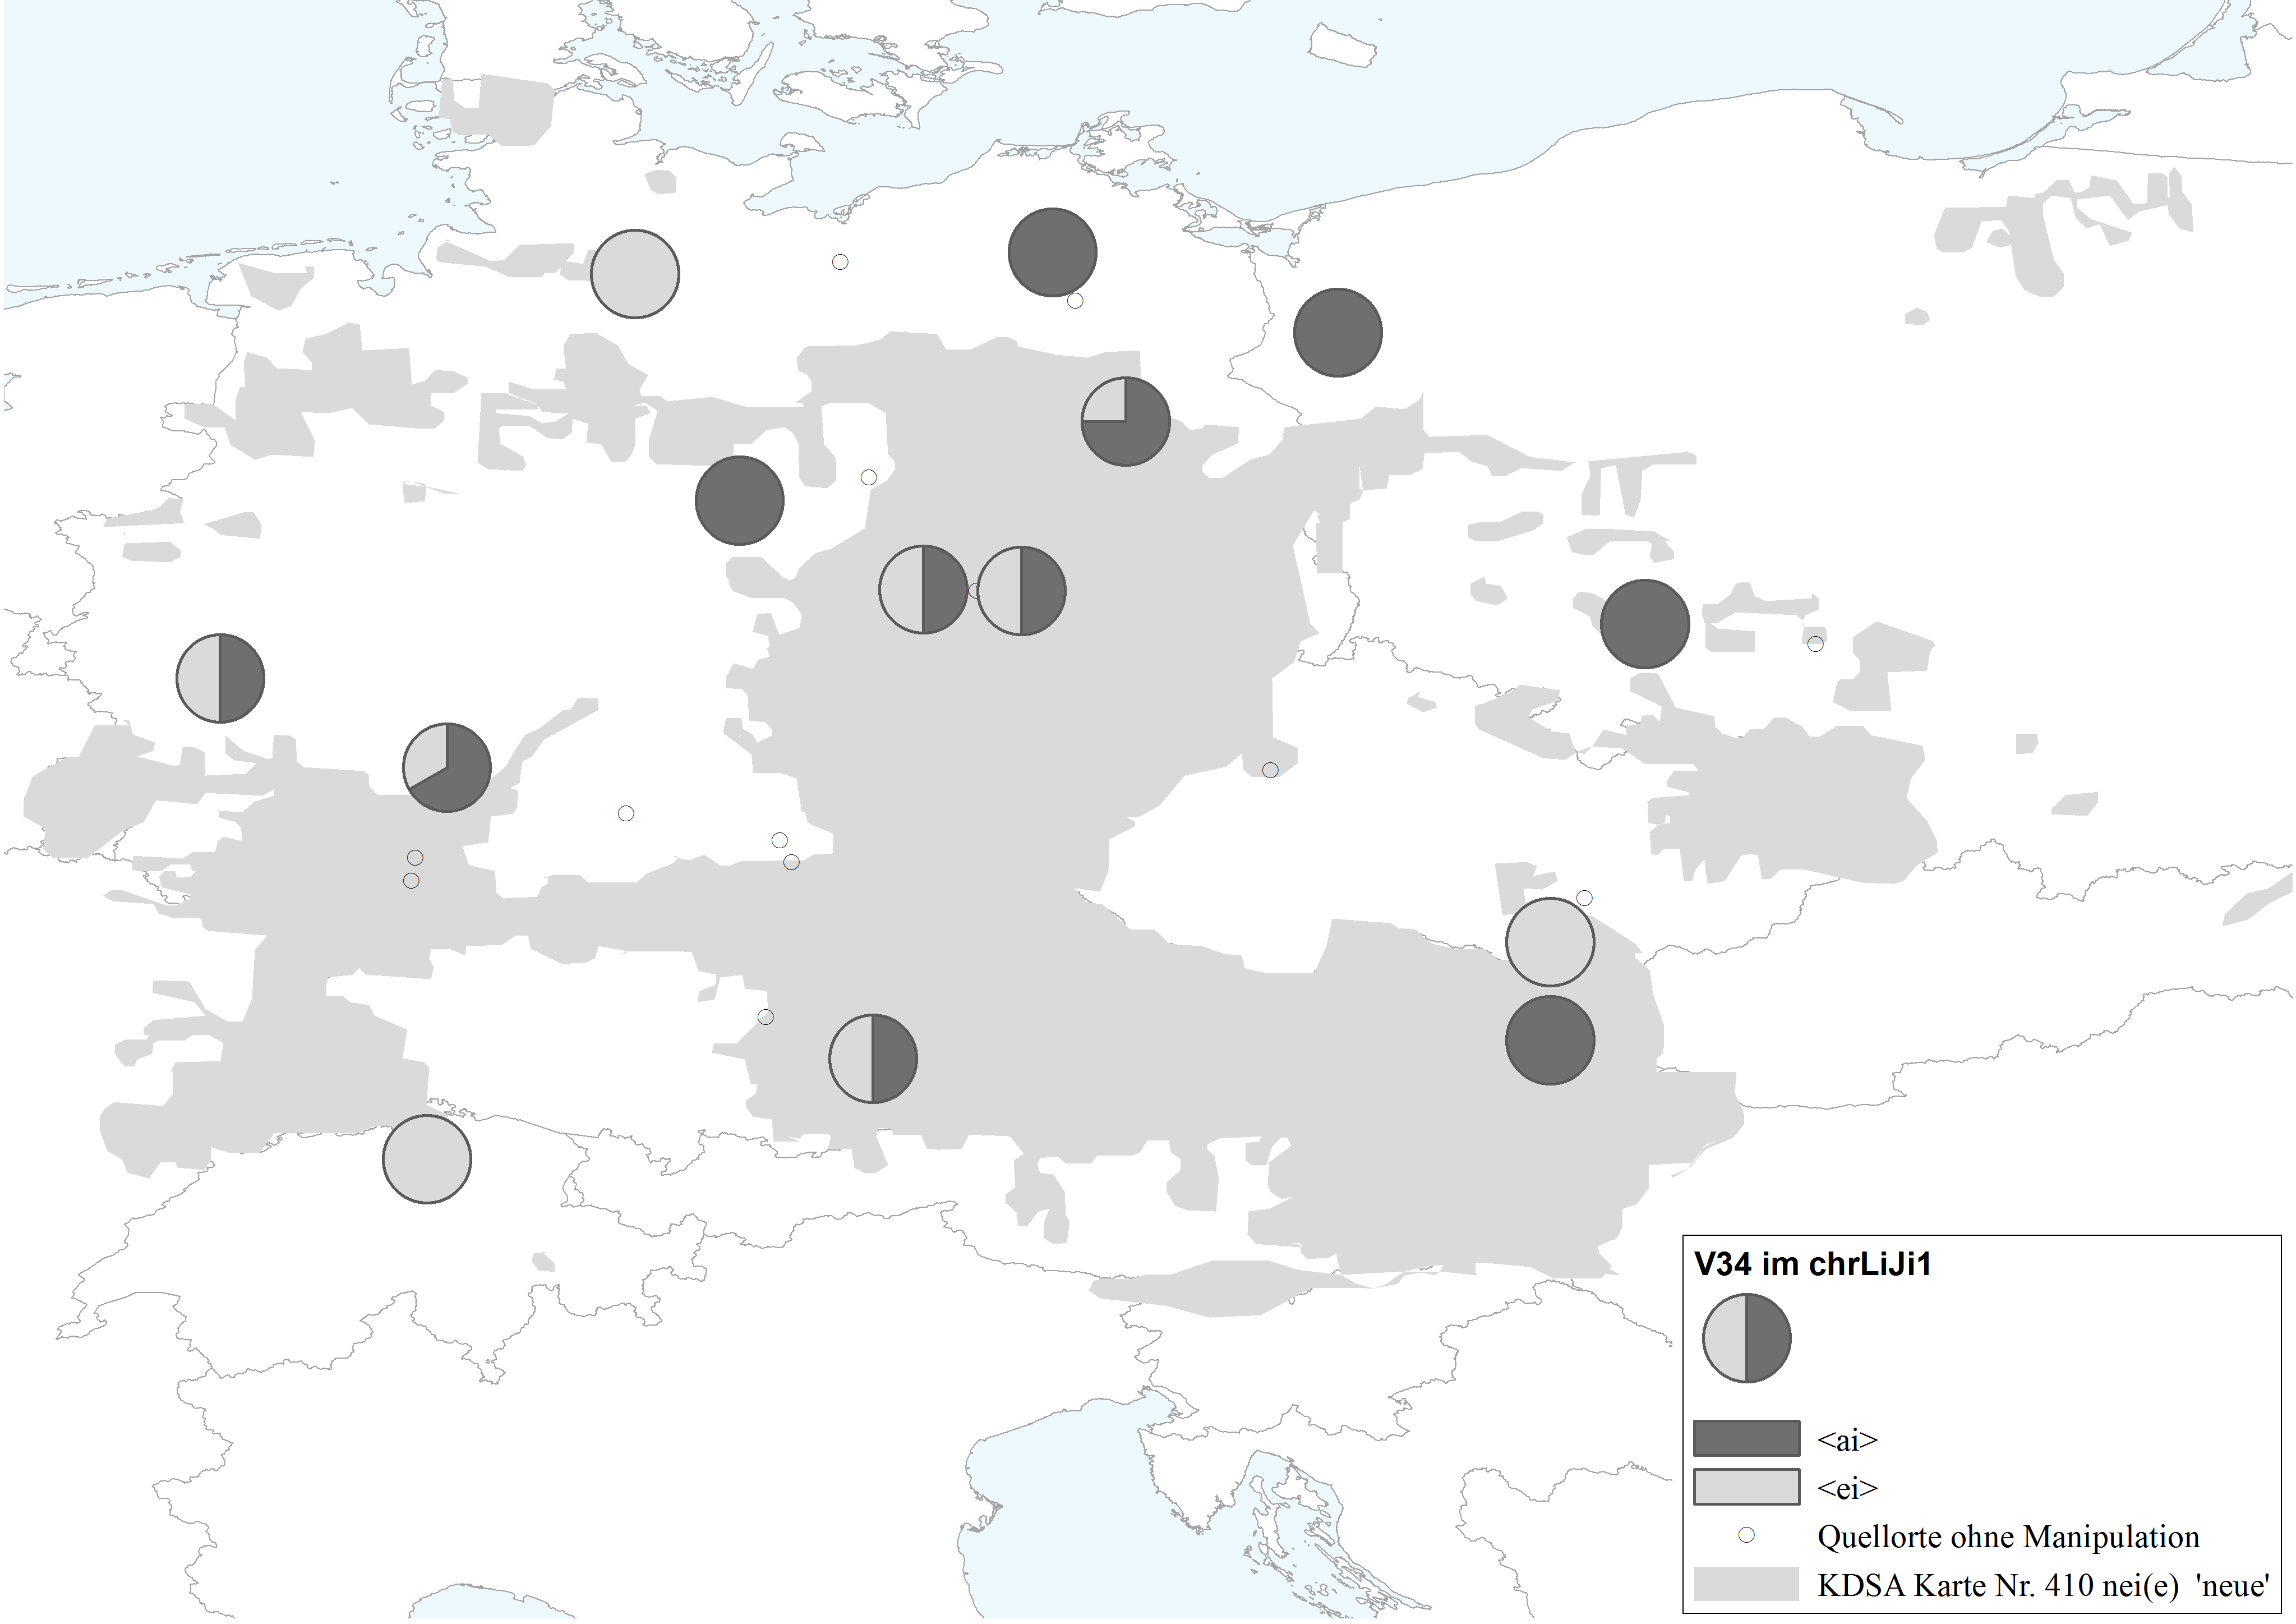
\includegraphics[scale=0.1]{figures/v34karte2.png}
		\caption{\label{karteV34}  \hai{V34} im \hai{chrLiJi1} mit \hai{KDSA} Karte Nr. 410}
		\end{figure}
\FloatBarrier
 

 
 
 Das \hai{jüdLiJi1} zeigt in acht Quellen den jiddischen Diphthong; in fünf von acht Fällen liegt die Schreibung <ei> vor und in drei von acht die mittels <ai>.\footnote{<ei> findet sich in \hai{GuS1,5,10}, \hai{PBreslau} u. \hai{PDebrecen}; <ai> findet sich in \hai{GuS23}, \hai{PBerlin2} u. \hai{PAlsleben}.}\\ 
 
 
 
  \section{/a/ > /o/ (\textit{a}-Verdumpfung)}\label{phonV1213}

Die \isi{Rundung} und Hebung von \textit{a} > \textit{o} wird hier vereinfachend als \quein{\textit{a}-Verdumpfung} bezeichnet. Im \hai{OJ} fiel \hai{V12} (urj. *\textit{\=\textopeno\textlengthmark, A\textsubscript{2}}, = mhd. \textit{â}, oj. \RL{יאָר} \textit{yor} \sem{Jahr}) und \hai{V13} (urj. *\textit{a} in offener Tonsilbe,  A\textsubscript{3}, = mhd. \textit{a}/\textit{â}, oj. \RL{שלאָגן} \textit{shlogn} \sem{schlagen}) zu /\textopeno\textlengthmark/ zusammen und wurde im \hai{ZOJ} zu /u\textlengthmark/ gehoben (\cite[93–121]{Timm1987}; \cite[186f]{Bin-Nun1973}). Im \hai{WJ} hingegen wurde lediglich \hai{V12} verdumpft; \hai{V13}, also *\textit{a} in offener Tonsilbe, blieb unverändert \parencite{Beider2010}. Abbildung \ref{karteV1213} zeigt, dass auch in den deutschen Dialekten die Verdumpfung im \hai{V13}-Kontext weniger präsent ist als die im \hai{V12}-Kontext und dass die Verdumpfung vorrangig in den östlichen Dialekten im Kontaktbereich zu slawischen (und finno-ugrischen) Sprachen stattgefunden hat. Dies könnte u.\,U. eine Erklärung dafür liefern, wieso diese Verdumpfung nur im \hai{OJ} stattgefunden hat. Andererseits ist die Situation in den westjiddischen Varietäten alles andere als klar, denn bislang ist lediglich das \hai{SWJ} der Schweiz ausreichend beschrieben worden (\cite{GuggenheimGruenberg1973}; \cite{Beider2010}).\footnote{Der \hai{LCAAJ} kartiert \hai{V13} nur am Beispiel eines hebr. Lexems (\cite[68]{Herzog1992}), was wenig aussagekräftig ist für die Situation der Germanismen.} Bislang fehlen Detailanalysen zu weiteren westjiddischen Dialekträumen.

Ein weiteres Problem, das sich bei diesem Phänomen ergibt, betrifft die Bestimmung eines Vokals als einem aus \hai{V12} hervorgegangenem. Die Analyse von \hai{V12} im \hai{WJ} führte in den bisherigen Arbeiten m.\,E. oft zu vorschnellen Schlüssen, da ein zu starkes Gewicht auf die gemeinsame Genese von Ost- und \ili{Westjiddisch} gelegt wurde. Die Karten des \hai{LCAAJ} (\citeyear[67]{Herzog1992}) und \citeauthor{GuggenheimGruenberg1973}s (\citeyear[60–64]{GuggenheimGruenberg1973}) geben an, dass \hai{V12} im westlichen Teil des \hai{WJ} als /\textopeno \textsubarch{u}/ oder /a\textsubarch{u}/ und im \hai{SÜJ} im westl. \hai{SWJ} als /\textopeno \textsubarch{\textsci}/ realisiert wurde (s.\,a. \cite{Beider2010}). Im \hai{WJ} beträfe dies nach den Daten des \hai{LCAAJ}s ohnehin nur einzelne (leider nicht näher angegebene) Wörter hebräischen Ursprungs. Für das \hai{SÜJ} und das westl. \hai{SWJ} sind zwar die einzelnen, überwiegend germanischstämmigen Lexeme gegeben (vgl. \cite{GuggenheimGruenberg1973}), doch bei diesen ist der mhd. Vokal nicht gänzlich geklärt. So werden etwa die Formen für \RL{דוי}  \sem{hier, da} und \RL{שלאָפן}  \sem{schlafen} angegeben. Diese Lexeme sind für das Mhd. aber sowohl als \textit{dô}, \textit{slôfen} wie auch als \textit{dâ}, \textit{slâfen} belegt \parencite[Bd. 1, Sp. 445]{Lexer1992}. Der Diphthong /\textopeno \textsubarch{u}/, bzw. /\textopeno \textsubarch{\textsci}/ im \hai{SÜJ}, kann damit aus \hai{V42} (= mhd. \textit{ô}) hervorgegangen sein, bei welchem eine solche Diphthongierung im \hai{WJ} stattgefunden hat (vgl. Abschnitt \ref{phonV42}; s.\,a. \cite[188]{Bin-Nun1973}). Dieser kann wiederum aus einer Verdumpfung von \textit{â} zustande gekommen sein.\footnote{Einige solcher Lexeme, die nach den Entwicklungen von \hai{V42} diphthongiert wurden (z.\,B. \sem{da}, \sem{ja}), wurden in dieser Arbeit auch als ein solches Phänomen analysiert und entsprechend nicht in die Daten zur \textit{a}-Verdumpfung aufgenommen (vgl. Abschnitt \ref{phonV42}). Nach \textcite[60f]{GuggenheimGruenberg1973} besteht im westl. \hai{SWJ} sogar gar keine Unterscheidung mehr zwischen \hai{V13}, \hai{V12} und \hai{V42}. Diese sind, zumindest in den kartierten Lexemen, unter dem Diphthong aus \hai{V42} zusammengefallen. Sie kartiert die Lexeme \sem{schlafen}, \sem{raten}, \sem{fragen} (> urj. *\textit{a} in offener Tonsilbe = \hai{V13} gemeinsam mit \sem{mal}, \sem{da} (> \hai{V12} bzw. \hai{V42}) als < mhd. \textit{â}. Siehe hierzu auch \textcite[115]{Timm1987}. Um aber die Situation der Verdumpfung und Diphthongierung im \hai{WJ} genau erfassen zu können, bedarf es einer Detailanalyse, die diese Arbeit nicht leisten kann.} Eine solche Vermutung müsste allerdings erklären, wieso im \hai{OJ} eine Diphthongierung nach dem Muster von \hai{V42} am verdumpften \hai{V12} nicht stattgefunden hat. Dieses Phänomen wäre also neben der Monophthongierung von \hai{V24} und \hai{V44} eine phonologische Entwicklung, in der sich \hai{WJ} und \hai{OJ} auseinander entwickelt haben. Darüber hinaus spiegelt die Situation der Vokale \hai{V11}, \hai{V12}, \hai{V13} und \hai{V42} in den germanischen Lexemen des Jiddischen den Umstand wider, dass es bereits im Mhd. (regionale) Variation bei der Verdumpfung von \textit{a}-Phonemen gegeben hat. In der deutschen Sprachgeschichte ist Verdumpfung von mhd. \textit{â} (einschließlich \textit{a} in offener Tonsilbe) ab dem 12. Jahrhundert in der Schriftsprache zunächst im Bairischen nachweisbar und greift im 13. und 14. Jahrhundert auf das Niederalemannische und die mitteldeutschen Dialekte  über (\cite[212]{Schirmunski1962}; \cite[§48]{Paul2007}; \cite[§L14]{Ebert1993}). Verdumpfungen \qu{treten in bestimmter konsonantischer Umgebung ein, ohne dass sich daraus eine feste Regel ableiten lässt} \parencite[§48]{Paul2007}. Damit ist  auch die Entwicklung im Deutschen nicht auf eine einfache Formel zu bringen. Sie ist in den modernen deutschen Dialekten mit Ausnahme des Höchstalemannischen und Nordniederdeutschen nahezu überall anzutreffen (\cite[212]{Schirmunski1962}; \cite[§L14]{Ebert1993}; vgl. Karte in Abb. \ref{karteV1213}). Die \textit{a}-Verdumpfung ist jedoch besonders lexemgebunden, so dass sie, v.\,a. bei hochfrequenten Lexemen, tatsächlich in allen Dialekten auftritt (vgl. u.\,a.\hai{WA} Karten Nr. 86, 117, 131, 244, 313, 338, 544).\footnote{Das Höchstalemannische zeigt sich trotzdem relativ konservativ. Im \hai{SDS} (Karte V/119) finden sich lediglich im Kanton Uri Hinweise auf eine Verdumpfung von \textit{â} in \sem{ja}. Generell gilt, dass die \qu{\textit{a}-Verdumpfungslinie} das Höchstalemannische von den anderen alemannischen Dialekten abgrenzt (vgl. \hai{SDS} Karte Nr. I/62).} Ein Erklärungsansatz für die Variation, die bereits im Mhd. vorliegt, wäre, sie als ein wesentlich älteres Phänomen der germanischen Sprachgeschichte zu verstehen. Bereits im Ahd. steht germ. \textit{a} als <o> oder auch parallel zu <a> \parencite[§ 25]{BrauneReiffenstein2004}. So ist das angenommene mhd. und urj. System der offenen und halboffenen Vokale kein ideales Referenzsystem. Im Fall des Jiddischen erschwert die \isi{Orthographie} besonders die Graphem-Phonem-Analyse, da <\RL{א}> sowohl für /a/ als auch für /\textopeno/ steht und nur in Sonderfällen /\textopeno/ als <\RL{ו}> 
erkennbar ist \parencite[93–121]{Timm1987}. Eine sinnvolle Bestimmung, welcher Vokal auf welchen der protojiddischen Vokale \hai{V42}, \hai{V12}, \hai{V11} und \hai{V13} zurückzuführen ist, ist so m.\,E. kaum möglich. 


Bevor die Situation der \textit{a}-Verdumpfung im \hai{WJ} geklärt ist, ergibt es wenig Sinn, die Durchführung einer Differenzierung zwischen \hai{V12}, \hai{V13} und \hai{V11} im Rahmen der Analyse des \hai{LiJi} zu untersuchen. Die Analyse des \hai{LiJi} macht es uns auch etwas einfacher, da die Manipulation von <a> zu <o> an der Standardorthographie des Neuhochdeutschen erfolgt, also an einem synchronen System, an dem die diachronen Strukturen kaum mehr erkennbar sind. Die Analyse kann also die Frage sicher beantworten, welche Quellen eine Verdumpfung von germ. \textit{a} zeigen; problematisch bleibt die genaue Bestimmung der mhd. und urj. Referenzvokale. 

So finden sich 34 Texte im \hai{chrLiJi1}, in denen <o> an der Position von <a> gesetzt wird. \hai{V11} (A\textsubscript{1}) < urj. *\textit{a\textlengthmark} bleibt erstaunlicherweise im \hai{chrLiJi1} überwiegend unbeeinflusst von der Verdumpfung. Lediglich am Verb \sem{fragen} findet sich <o> in fünf Texten. Die Verdumpfung im \hai{LiJi1} betrifft immer nur das Verb, nie das Substantiv. Die entsprechenden Quellen sind \hai{GW} (n.a., ca. 1900), \hai{JK} (Breslau, 1810), \hai{LB} (Berlin, 1785), \hai{MV} (Berlin, 1862) u. \hai{SV} (München, 1890). Doch auch hier ist der mhd. Ausgangsvokal problematisch: mhd. \textit{vrâgen} (= \hai{V11}) ist ebenso belegt wie \textit{frôgen} (= \hai{V42}) \parencite[Bd. 3, Sp. 487]{Lexer1992}. Ein Beleg für die \textit{a}-Verdumpfung in \sem{fragen} könnte demnach auch lediglich auf die  Wiedergabe des ursprünglichen Langvokals von \hai{V42} schließen. Ein weiteres Argument, wieso man dieses Lexem eher nicht als Beleg einer Verdumpfung von \hai{V11} zählen sollte, findet sich in \textcite[60f]{GuggenheimGruenberg1973}: Sie kartiert \textit{frougen} nicht als Beleg für ein \hai{V11}-Lexem, sondern  es findet sich in Belegen für die von ihr angenommene Diphthongierung von \hai{V12} im \hai{SWJ}, die ich  generell als eine Missinterpretation von \hai{V42}-Vokalen ansehe (s.\,o.).\footnote{Im modernen \hai{OJ} hat sich das Substantiv  \RL{פרא\makebox(-1.5,-7.5)[r]{\libertineGlyph{uni207B}}גע} \sem{Frage} aus \hai{V11} entwickelt und blieb unverdumpft. Im modernen \hai{OJ} hat sich die \isi{Wechselflexion} auf dieses Verb analogisch ausgedehnt – bereits in mhd. als \textit{vrëgen} belegt  \parencite[Bd. 3, Sp. 487]{Lexer1992} – und im \hai{NOJ} und \hai{SOJ} folgt es der Diphthongierung von \hai{V22}  \RL{פרייגן}.} Das Lexem \sem{fragen} zeigt zweierlei. Erstens sind die phonologischen Arbeiten zum Jiddischen sehr uneinheitlich in der Verwendung des protojiddischen Systems. Zweitens, und dieses Problem wiegt deutlich schwerer, weisen damit einzelne Lexeme in unterschiedlichen regionalen Varietäten des Jiddischen auch unterschiedliche protojiddische Ausgangsvokale auf. Dies aber hieße, dass die regionalen Varietäten älter sind als angenommen, was wiederum bedeute, dass das protojiddische System noch längst nicht ausgereift war. Ob wir es in diesem Fall mit einer Hyperkorrektur zu tun haben, ist letzten Endes schwer zu entscheiden. Eine weitere mögliche Hyperkorrektur  findet sich in einer Wiener Quelle im Beleg \textit{Nocht} \sem{Nacht} (\hai{AO} Wien, 1770:\,134). Dieser Beleg ist auf einen Einfluss des deutschen Dialekts zurückzuführen. Im Mittelbairischen ist diese Form weit verbreitet (\hai{WEK} Karte \sem{die Nacht}). In allen anderen Korpusbelegen betrifft die Verdumpfung ausschließlich die historischen Vokale \hai{V12} und \hai{V13}. Unter starkem Vorbehalt kann gesagt werden, dass \hai{chrLiJi1} vorwiegend Verdumpfungen in Lexemen vornimmt, in denen auch im Jiddischen verdumpft wird. 

Der historische Querschnitt zeigt eine besondere Anhäufung der \isi{a-Verdumpfung} in Quellen zwischen 1774 und 1835 (Abb. \ref{histoV1213}). Danach gibt es eine Phase, in der die Verdumpfung in manchen Quellen durchgeführt wurde, in anderen aber nicht belegt ist. In allen Quellen der Jahrhundertwende um 1900 ist sie dann ausschließlich präsent, wird aber in den drei jüngsten Texten des \isi{Korpus} nicht umgesetzt.
  
    %%%V12/13Diagramm%\begin{flushleft}	
\begin{figure}[h!]
	\begin{tikzpicture}
		\begin{axis}[only marks, width=0.82\textwidth,height=0.2\textheight,
		legend style={at={(1,1)},xshift=+0.2cm, yshift=-0.7cm,anchor=north west,nodes=left},
			%title={Funktionstypen des sp\"aten Westjiddisch},
			xtick={1700, 1725, 1750, 1775, 1800, 1825, 1850, 1875, 1900, 1925, 1950, 1975}, ytick=\empty,
			x tick label style={/pgf/number format/1000 sep=}, 
			y tick label style={/pgf/number format/1000 sep=},
			%extra y ticks={456.1, 1022.4},
			%extra y tick labels={{456,1},{1022,4}},
			extra y tick style={grid=major,
				tick label style={, ,}},
				ymin=0.7,
				ymax=2.9,
			ylabel={Phänomenbelege},
			enlarge x limits=0.03]	
	
			
\addplot [mark=*, black] table [x=jahr, y=V1213] {figures/V1213.txt}; %2

\addplot [mark=o, black] table [x=jahr, y=no] {figures/V1213no.txt}; %1.5


 

			% Andere Formen a={mark=square*,blue},% b={mark=triangle*,red},% c={mark=o,draw=black}}
						\legend{\hai{V12}/\hai{V13} als <o>, unmanipuliert} %macht Legende
		\end{axis}
	\end{tikzpicture}
	\caption{\hai{V12} und \hai{V13} im \hai{chrLiJi1}}
	\label{histoV1213}	
\end{figure}
\FloatBarrier
  
  
  
Die Kartierung der Belege zeigt in erster Linie, in welchem großflächigen Gebiet die Verdumpfung, insbesondere die von \hai{V13}, in den deutschen Mundarten stattgefunden hat (Abb. \ref{karteV1213}). Einzig zwei Quellorte im niederdeutschen Raum, zeigen mit der Verdumpfung ein in den örtlichen deutschen Varietäten weniger verbreitetes Phänomen. So fungiert sie möglicherweise nicht als expliziter Identifikator für die jiddische Sprache, sondern soll evtl. generell Dialektalität transportieren. \\


\begin{figure}[h!]
		\centering
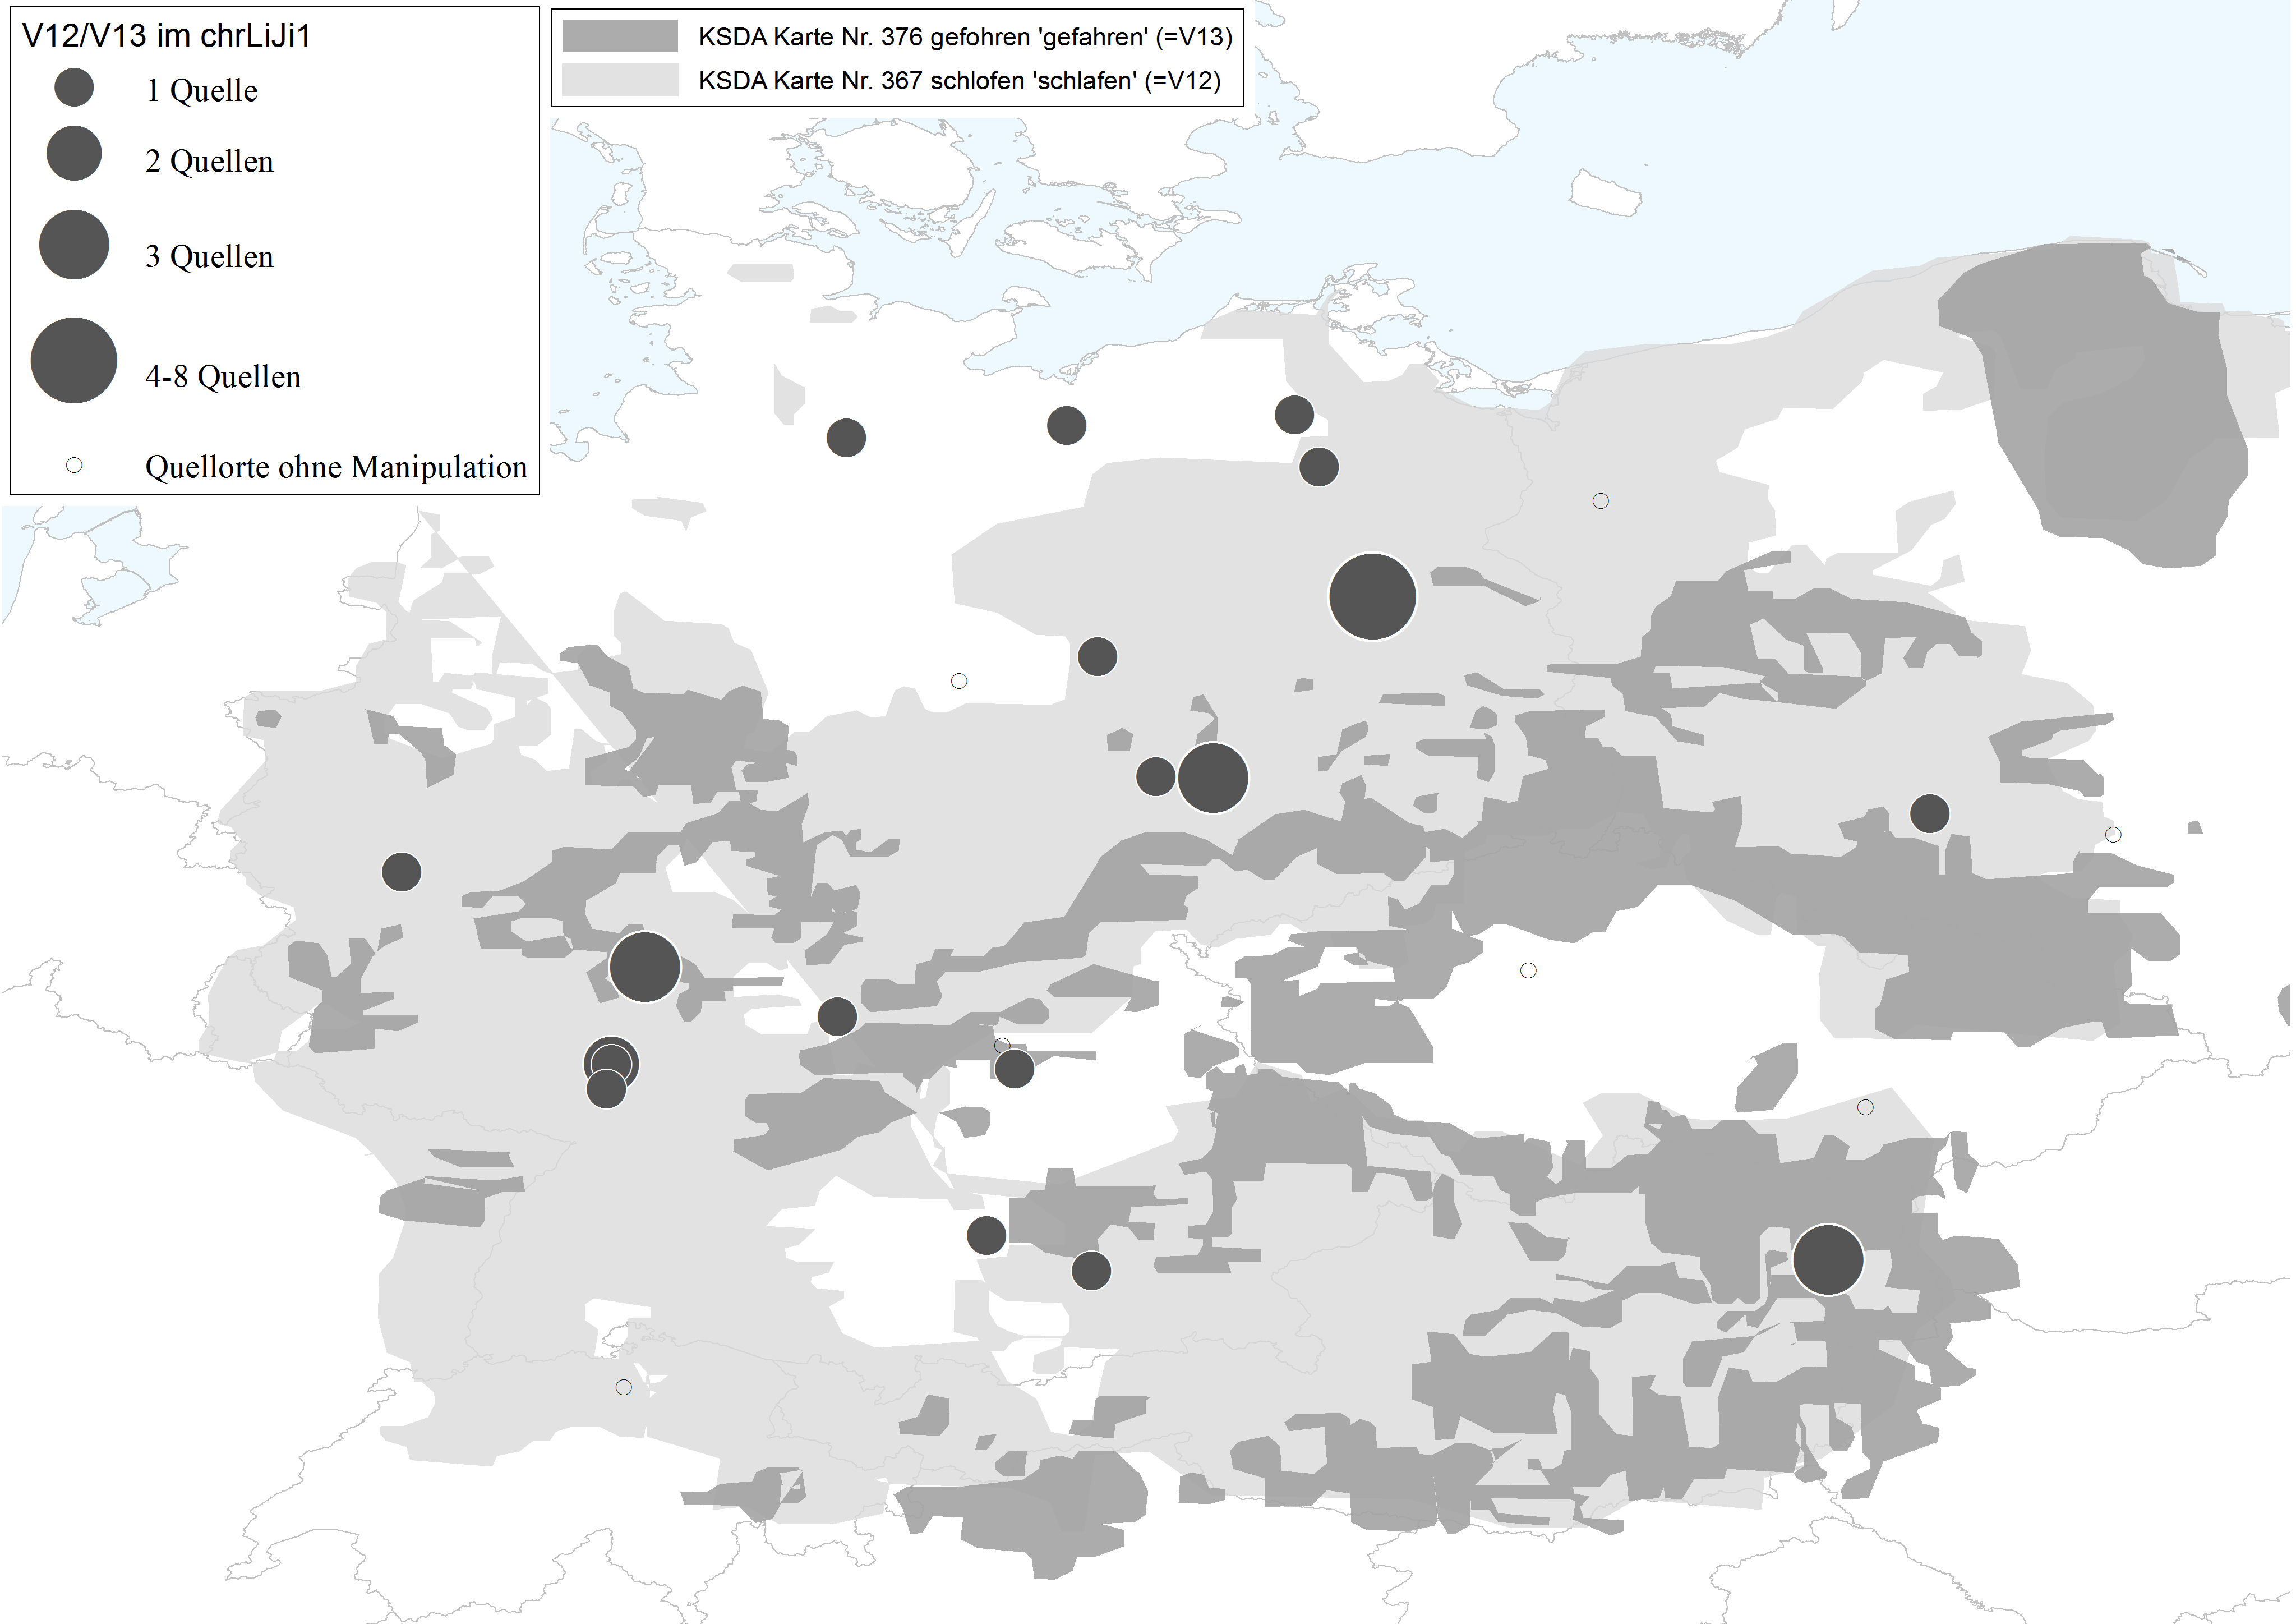
\includegraphics[scale=0.1]{figures/karteV1213_2.png}
		\caption{\label{karteV1213}  \hai{V12}/\hai{V13} im \hai{chrLiJi1} mit \hai{KDSA} Karten Nr. 376, 367}
		\end{figure}
\FloatBarrier

  
  
  
 Auch im \hai{jüdLiJi1} finden sich die Verdumpfung von \hai{V12} und \hai{V13}. Alle Texte, bis auf einen,\footnote{Dabei handelt es sich um die Quelle \hai{PBerlin1}.}  zeigen <o> an der Position von \hai{V12}. In zwei Quellen ist jedoch die Verdumpfung von \hai{V11} am Lexem \sem{fragen} belegt (\hai{GuS23}:\,5, 6; \hai{PAlsleben}:\,3) und damit an demselben Lexem, welches auch im \hai{chrLiJi1}  in dieser Form auftritt (s.\,o.). 
 
 
 Da die Verdumpfung ein für Muttersprachler des Deutschen recht zugängliches Phänomen ist, überrascht es, dass Hyperkorrekturen, also die Verdumpfung von \hai{V11}, wie etwa \textit{Sproche} \sem{Sprache} oder \textit{Gost} \sem{Gast}, nicht häufiger auftreten. Dass dies nicht der Fall ist, spricht m.\,E. ganz besonders für die Akkuratheit der Imitationen, egal in welchem Stadium des \hai{LiJi}. Die Verdumpfung von \hai{V11} hat in den deutschen Dialekten zwar seltener stattgefunden, als diejenige von \hai{V12} und \hai{V13}, ist aber besonders in mitteldeutschen und bairischen Varietäten gegeben (vgl. \hai{WA} Karte Nr. 360  \sem{Nacht} u. \hai{WEK} Nr. \sem{diese Nacht}). Ein Einfluss der Matrixsprache der Autoren auf die Verdumpfung ist demnach weitestgehend auszuschließen. Eine zwischen \hai{V12} und \hai{V13} (und \hai{V42}) näher differenzierende Analyse bedarf jedoch Grundlagenarbeit zum mittelhochdeutschen, protojiddischen und westjiddischen Vokalsystem.\\
  
   
  
 \section{\textit{o} > \textit{u} und \textit{u} > \textit{o}}\label{o_u_zeug}

Die zwei komplementären Entwicklungen der Hebung von \textit{o} und der Senkung von \textit{u} sind ein bekanntes Phänomen der ostjiddischen Dialekte. Für das \hai{WJ} fehlen allerdings noch immer flächendeckende Untersuchungen. Mit Hilfe des \hai{LiJi} wollen die folgenden Unterabschnitte zeigen, dass Hebung und Senkung aber nicht auf das ostjiddische Dialektgebiet beschränkte Ereignisse sind.\\


 \subsection{Hebung von /\textit{o}/ > /\textit{u}/ (vor Nasal)}\label{o_u} 

 Ein Charakteristikum des \hai{ZOJ} und \hai{SOJ} ist die Hebung von \hai{V12} und die Verdumpfung von \hai{V13} > /\textit{u}/ (\cite[66]{Herzog1992}; \cite[28]{Beider2010}). Die Karte des \hai{LCAAJ} (\citeyear[66–68]{Herzog1992}), zeigt, dass dieses Phänomen auch vereinzelt Hebraismen das \hai{WJ} betroffen hat. Eine Detailanalyse zur Situation im \hai{WJ} steht jedoch noch aus. Immerhin zeigt eine der authentischsten Quellen des \hai{ZWJ}, \qu{Die Hochzeit zu Grobsdorf} (1822), diese Hebung von /\textit{o}/ > /\textit{u}/ mehrfach, wie z.\,B. am Verb \sem{kommen} (\ref{bspgrob1}) oder den Präpositionen \sem{von} (\ref{bspgrob2}) und \sem{wo} (\ref{bspgrob3}). Diese Hebung hat in den koterritorialen zentralhessischen Dialekten nicht stattgefunden sondern überwiegend die ostmitteldeutschen, rheinfränkischen, alemannischen Dialekte sowie das Südbairische des Burgenlands betroffen (vgl. Karte \ref{karteou}; \hai{SDS} Karte Nr. I/46; \hai{WEK} \sem{solche}). Dementsprechend korrekt ist sie auch nicht in den Passagen aus \qu{\RL{דיע האָכצייט צו גראָבסדאָרף}} (\sem{Die Hochzeit zu Grobsdorf}) umgesetzt, in denen nicht-jüdische Bevölkerung spricht (\ref{bspgrob4}). Als eine weitere Quelle, die diese Hebung zeigt, sei Wolfssohns maskilisches Stück \qu{\RL{לייכטזין אונד פֿרעממעלייא}}  (\sem{Leichtsinn und Frömmelei}) angeführt (Bsp. \ref{bspleicht2}). So darf angenommen werden, dass die Hebung von /\textit{o}/ > /\textit{u}/ teilweise auch im \hai{WJ} stattgefunden hat.\\

 \eenumsentence{
	\item \RL{ עס קוממע נאָך גא\makebox(-1.5,-7.5)[r]{\libertineGlyph{uni207B}}ר פֿיעל לייט.
 } \\
\textit{es kumme nokh gar fiel leyt}\\
\sem{Es kommen noch gar viele Leute} 
	\\ (\qu{Die Hochzeit zu Grobsdorf} 1822:\,15)
\label{bspgrob1} 

	\item \RL{ דאָס דוא פון גראָבסדארף ביסט.
 }
	\\
	\textit{dos du fun grobsdorf bist}\\
	\sem{dass du von/aus Grobsdorf bist}
	 \\ (\qu{Die Hochzeit zu Grobsdorf} 1822:\,9)
\label{bspgrob2} 

\item \RL{ וואו האָט מער זונסט געוויסט פֿון פֿערליעבע!
 }
	\\
	\textit{vu hot mer zunst gevist fun ferliebe!}\\
	\sem{wo hat man sonst vom Verlieben gehört!}
	 \\ (\qu{Die Hochzeit zu Grobsdorf} 1822:\,14)
\label{bspgrob3} 



\item \RL{דֵיע זאָ אים לעבע פֿירקאָממע
 }
	\\
	\textit{deie so im lebe firkomme}\\
	\sem{die so im Leben vorkommen}
	 \\ (\qu{Die Hochzeit zu Grobsdorf} 1822:\,5)
\label{bspgrob4} 


\item \RL{נאָרר ער מעכט גערן ען אויסרייד האָבן אין דער קיך צו קוממען
 } \\
\textit{nor er mekht gern en ousreyd/ausreyd hobn in der kikh zu kummen}\\
\sem{nur möchte er eine Ausrede haben, um in die Küche zu kommen}
	\\ (\qu{Leichtsinn und Frömmelei} 1795/96:\,49)
\label{bspleicht2} 

          }
    
 Für eine Existenz der Hebung im \hai{WJ} sprechen auch die Daten des \hai{jüdLiJi1}: Sieben der zehn Quellen weisen diese auf.\footnote{\label{FNo_u}Dabei handelt es sich um die Quellen \hai{GuS1}, \hai{GuS5}, \hai{GuS10}, \hai{GuS23}, \hai{PAlsleben}, \hai{PBerlin1} u. \hai{PBreslau}.} Natürlich stehen diese Quellen schon allein aufgrund ihrer geographischen Verortung im Osten des westjiddischen Sprachgebietes, unter Verdacht ostjiddische Formen zu transportieren, doch ob dies der Fall ist, kann erst die abschließende Zusammenschau aller Phänomene entscheiden. %Im \hai{LiJi2}, welches sich am \hai{OJ} und insbesondere an zentralostjiddischen Dialekten orientiert, tritt diese Hebung in fünf Quellen auf.\footnote{Die Hebung ist in den Quellen \hai{TFReng}, \hai{WWR} mehrfach zu finden; in einzelnen Lexemen tritt sie nur in \hai{MAUeng}, \hai{MAUdt} u. \hai{DTL} in Erscheinung.} 
             
Von den Quellen des \hai{chrLiJi1} zeigen 17 Texte eine Hebung von /\textit{o}/ > /\textit{u}/. Wie das Histogramm in Abbildung \ref{histoo_u} zeigt, taucht es vor allem im Zeitraum zwischen 1770 und 1870 auf, kommt auch noch in den Quellen der Jahrhundertwende zum 20. Jahrhundert vor. \\

	
\begin{figure}[h!]
	\begin{tikzpicture}
		\begin{axis}[only marks, width=0.82\textwidth,height=0.2\textheight,
		legend style={at={(1,1)},xshift=+0.2cm, yshift=-0.7cm,anchor=north west,nodes=left},
			%title={Funktionstypen des sp\"aten Westjiddisch},
			xtick={1700, 1725, 1750, 1775, 1800, 1825, 1850, 1875, 1900, 1925, 1950, 1975}, ytick=\empty,
			x tick label style={/pgf/number format/1000 sep=}, 
			y tick label style={/pgf/number format/1000 sep=},
			%extra y ticks={456.1, 1022.4},
			%extra y tick labels={{456,1},{1022,4}},
			extra y tick style={grid=major,
				tick label style={, ,}},
				ymin=0.7,
				ymax=2.9,
			ylabel={Phänomenbelege},
			enlarge x limits=0.03]	
	
			
\addplot [mark=*, black] table [x=jahr, y=phaen] {figures/o_u.txt}; %2

\addplot [mark=o, black] table [x=jahr, y=no] {figures/o_u_no.txt}; %1.5

						\legend{Hebung /\textit{o}/ > /\textit{u}/, unmanipuliert} %macht Legende
		\end{axis}
	\end{tikzpicture}
	\caption{Die Hebung von /\textit{o}/ > /\textit{u}/ im \hai{chrLiJi1}}
	\label{histoo_u}	
\end{figure}
\FloatBarrier


Dieses Phänomen scheint besonders lexemgebunden zu sein. So findet man es im \hai{chrLiJi1} überwiegend am \isi{Infinitiv} von \sem{kommen}, der Präpositionen \sem{von} und \sem{wo} (vgl. \ref{bspgrob1}--\ref{bspgrob3}) und nur in Einzelbelegen an anderen Lexemen, z.\,B. \textit{Wuchen} \sem{Wochen} (\hai{AK} Zürich, 1948:\,219, 236), \textit{Sunn} \sem{Sonne} (\hai{DW} Wien, 1773:\,66; \hai{MV} Berlin, 1862:\,152R), \textit{Trummler} \sem{Trommler} (\hai{FS} Schwerin, 1805:\,73). 

Im \hai{chrLiJi1} tritt sie überwiegend an Quellorten in Erscheinung, an denen sie im deutschen Dialekt ebenfalls stattgefunden hat. Es kann demnach nicht entschieden werden, ob hier eine tatsächlich westjiddische Form wiedergegeben wird oder die des örtlichen deutschen Dialekts. Lediglich drei Quellorte (Berlin, Stavenhagen, Zürich) weisen die Hebung auf. Doch gerade in den Großstädten und in polnischer Grenznähe kann ein Einfluss des \hai{OJ} nicht vollständig ausgeschlossen werden. \\

 \begin{figure}[h!]
		\centering
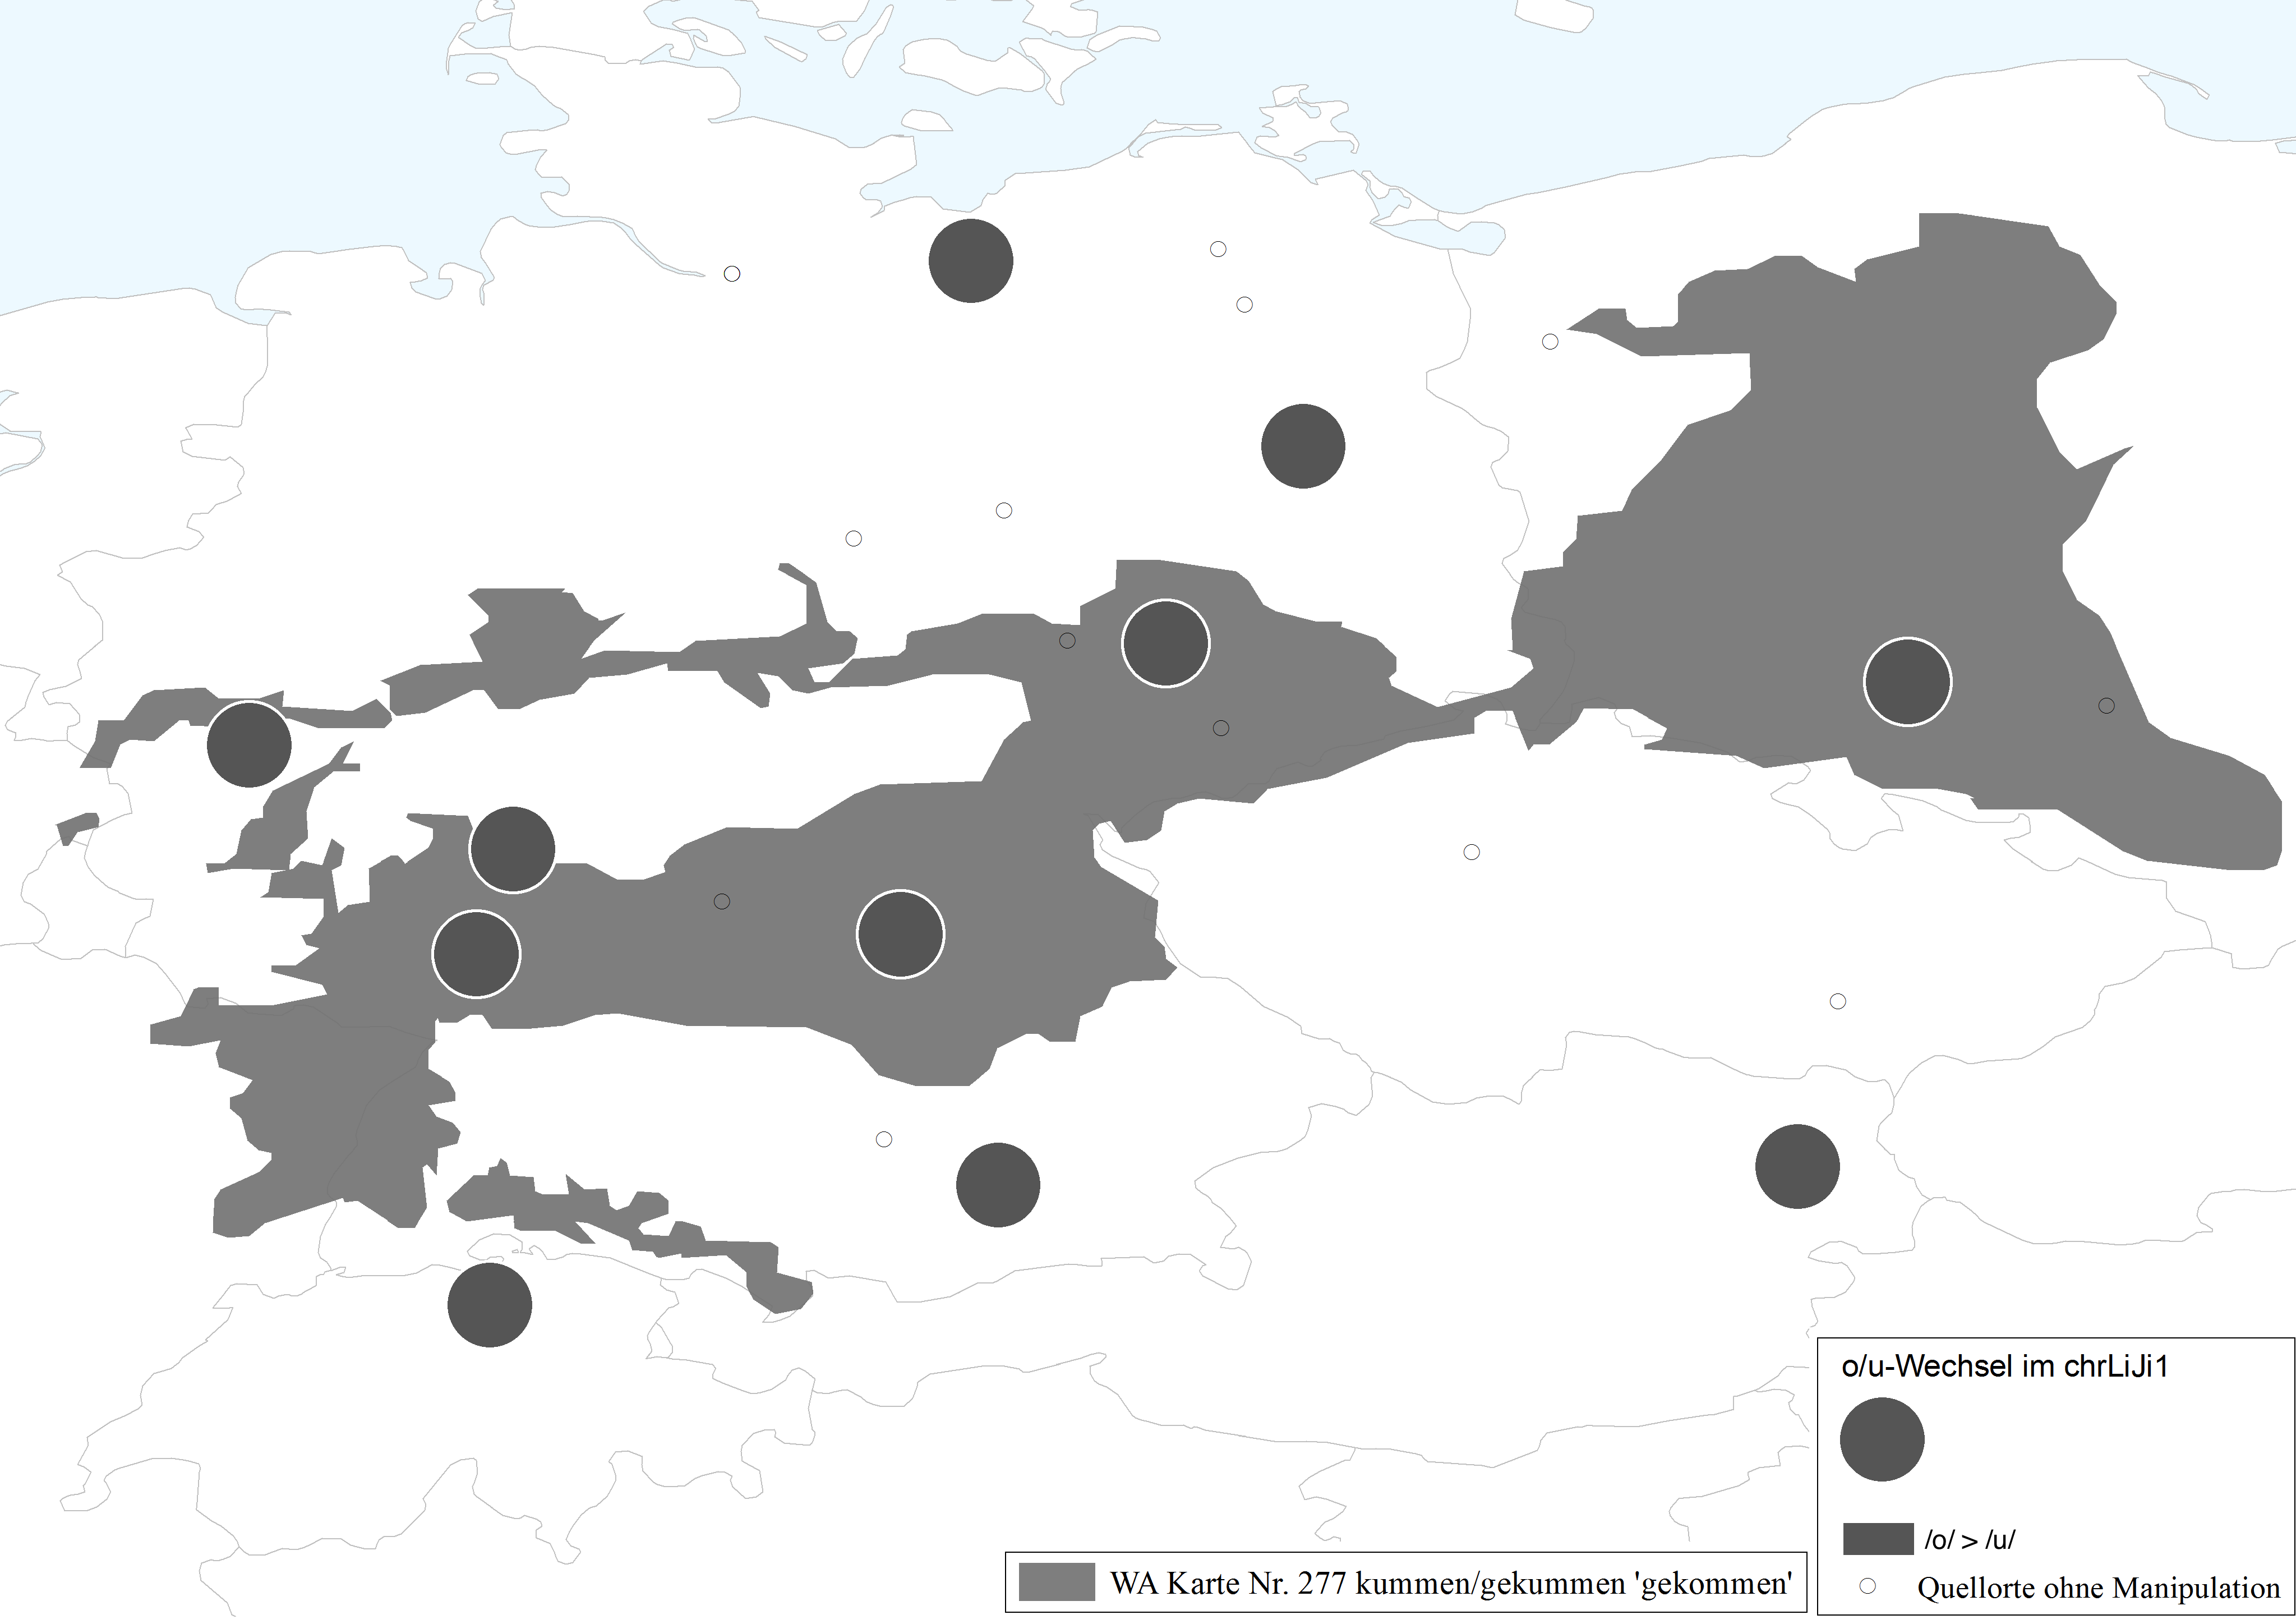
\includegraphics[scale=0.1]{figures/karteou2.png}
		\caption{\label{karteou} o > u im \hai{chrLiJi1} mit \hai{WA} Karte Nr. 277}
		\end{figure}
\FloatBarrier
		
		




 
 \subsection{Senkung von /\textit{u}/ > /\textit{o}/} \label{u_o} 
 %  %\noindent
Im \hai{ZOJ} und westlichen Teil des \hai{SOJ} hat eine Senkung von \hai{V51} (vor Liquid)  > /\textit{o}/ stattgefunden (\cite[84]{Herzog1992}). 
Zum \hai{WJ} liegen dem \hai{LCAAJ} \qu{no information} vor (\cite[84]{Herzog1992}). Wieder kann \qu{Die Hochzeit zu Grobsdorf} helfen, das Bild vom \hai{WJ} zu erweitern. Wie Bsp. \ref{bspgrob5}–\ref{bspgrob6} zeigen, finden wir dort parallel zur Hebung von /\textit{o}/ > /\textit{u}/ die Senkung von /\textit{u}/ > /\textit{o}/. Im \hai{ZWJ} des als \quein{Fürther Megille} bekannten Stücks \qu{\RL{אסתר. אָדער דיע בעלאָהנטע טוגענד}}  (\sem{Esther. Oder die belohnte Tugend}; Bsp. \ref{bspesther1}) wie auch im geographisch zwischen \hai{ZWJ} und \hai{SÜJ} schwer verortbarem (vgl. \cite[421]{FleischerSchaefer2012}) Stück \qu{\RL{לייכטזין אונד פֿרעממעלייא}} (\sem{Leichtsinn und Frömmelei}; Bsp. \ref{bspleicht1}) lässt sich diese Senkung finden. Allem Anschein nach sind die hier behandelte Hebung und Senkung jedoch vorrangig  Phänomene des \hai{ZWJ}, jedenfalls konnten keine Belege aus anderen Dialektregionen gefunden werden. Eine Einzelanalyse zur Situation im \hai{WJ} steht allerdings noch aus, um dies mit Gewissheit sagen zu können.\\


 \eenumsentence{
	\item \RL{ דוא זאָללסט ניקס צו קאָרץ קוממע
 } \\
\textit{du zollst niks zu korts kumme}\\
\sem{Du sollst nicht zu kurz kommen} 
	\\ (\qu{Die Hochzeit zu Grobsdorf} 1822:\,108)
\label{bspgrob5} 


\item \RL{דאָרך שא\makebox(-1.5,-7.5)[r]{\libertineGlyph{uni207B}}רע ווערד מער קלוג
 } \\
\textit{dorkh share verd mer klug}\\
\sem{Durch Schaden wird man klug} 
	\\ (\qu{Die Hochzeit zu Grobsdorf} 1822:\,12)
\label{bspgrob6} 




\item \RL{דוי גיהט נאָר ניט ריין אין דער שטוב
 } \\
\textit{dou/dau giht nor nit reyn in der shtub}\\
\sem{da geht nur nicht herein in die Stube}
	\\ (\qu{Esther. Oder die belohnte Tugend} 1828:\,56)
\label{bspesther1} 


\item \RL{נאָרר ער מעכט גערן ען אויסרייד האָבן אין דער קיך צו קוממען
 } \\
\textit{nor er mekht gern en ousreyd/ausreyd hobn in der kikh zu kummen}\\
\sem{nur möchte er eine Ausrede haben, um in die Küche zu kommen}
	\\ (\qu{Leichtsinn und Frömmelei} 1795/96:\,49)
\label{bspleicht1} 


}

Diese Senkung fand allerdings auch in den koterritorialen süd-zentralhessichen Mundarten statt und könnte daher in \qu{Der Hochzeit zu Grobsdorf} ein Interferenzereignis darstellen. Allgemein ist die Senkung in den deutschen Dialekten von /\textit{u}/ > /\textit{o}/ weitaus weniger verbreitet als die Hebung zu /\textit{u}/ (Karten in Abb. \ref{karteuo} u. \ref{karteouuoall}). Die Senkung fand neben dem Zentralhessischen vor allem im Rhein- und Moselfränkischen, in Teilen des Obersächsischen und Ostfälischen, im Westen der deutschsprachigen Schweiz (\hai{SDS} Karte Nr. I/51) sowie verstreut im Schlesischen und anderen Siedlungsmundarten statt. 

Die 14 Quellen des \hai{chrLiJi1}, welche die Senkung zeigen, finden sich überwiegend in der ersten Hälfte des 19. Jahrhunderts, später tritt die Senkung aber immernoch regelmäßig auf (Abb. \ref{histou_o}). \\


 %%%u > o Diagramm%\begin{flushleft}	
\begin{figure}[h!]
	\begin{tikzpicture}
		\begin{axis}[only marks, width=0.82\textwidth,height=0.2\textheight,
		legend style={at={(1,1)},xshift=+0.2cm, yshift=-0.6cm,anchor=north west,nodes=left},
			%title={Funktionstypen des sp\"aten Westjiddisch},
			xtick={1700, 1725, 1750, 1775, 1800, 1825, 1850, 1875, 1900, 1925, 1950, 1975}, ytick=\empty,
			x tick label style={/pgf/number format/1000 sep=}, 
			y tick label style={/pgf/number format/1000 sep=},
			%extra y ticks={456.1, 1022.4},
			%extra y tick labels={{456,1},{1022,4}},
			extra y tick style={grid=major,
				tick label style={, ,}},
				ymin=0.7,
				ymax=2.9,
			ylabel={Phänomenbelege},
			enlarge x limits=0.03]	
	
			
\addplot [mark=*, black] table [x=jahr, y=phaen] {figures/u_o.txt}; %2

\addplot [mark=o, black] table [x=jahr, y=no] {figures/u_o_no.txt}; %1.5


 

			% Andere Formen a={mark=square*,blue},% b={mark=triangle*,red},% c={mark=o,draw=black}}
						\legend{Senkung /\textit{u}/ > /\textit{o}/, unmanipuliert} %macht Legende
		\end{axis}
	\end{tikzpicture}
	\caption{Die Senkung von /\textit{u}/ > /\textit{o}/ im \hai{chrLiJi1}}
	\label{histou_o}	
\end{figure}
\FloatBarrier



Die Kartierung der Korpusbelege zeigt, dass die Senkung vermehrt auch in Regionen durchgeführt wurde, in denen sie in den deutschen Mundarten unüblich ist (Abb. \ref{karteuo}). Viele Belegorte, die in einem Gebiet liegen, in welchem die Senkung im Deutschen belegt ist, zeigen allerdings keine Manipulation von /\textit{u}/ > /\textit{o}/ im \hai{chrLiJi1}, dies schwächt einen Erklärungsversuch auf Basis eines potentiellen Einflusses der deutschen Dialekte auf das \hai{chrLiJi1} zusätzlich ab.  \\
 
  \begin{figure}[h!]
		\centering
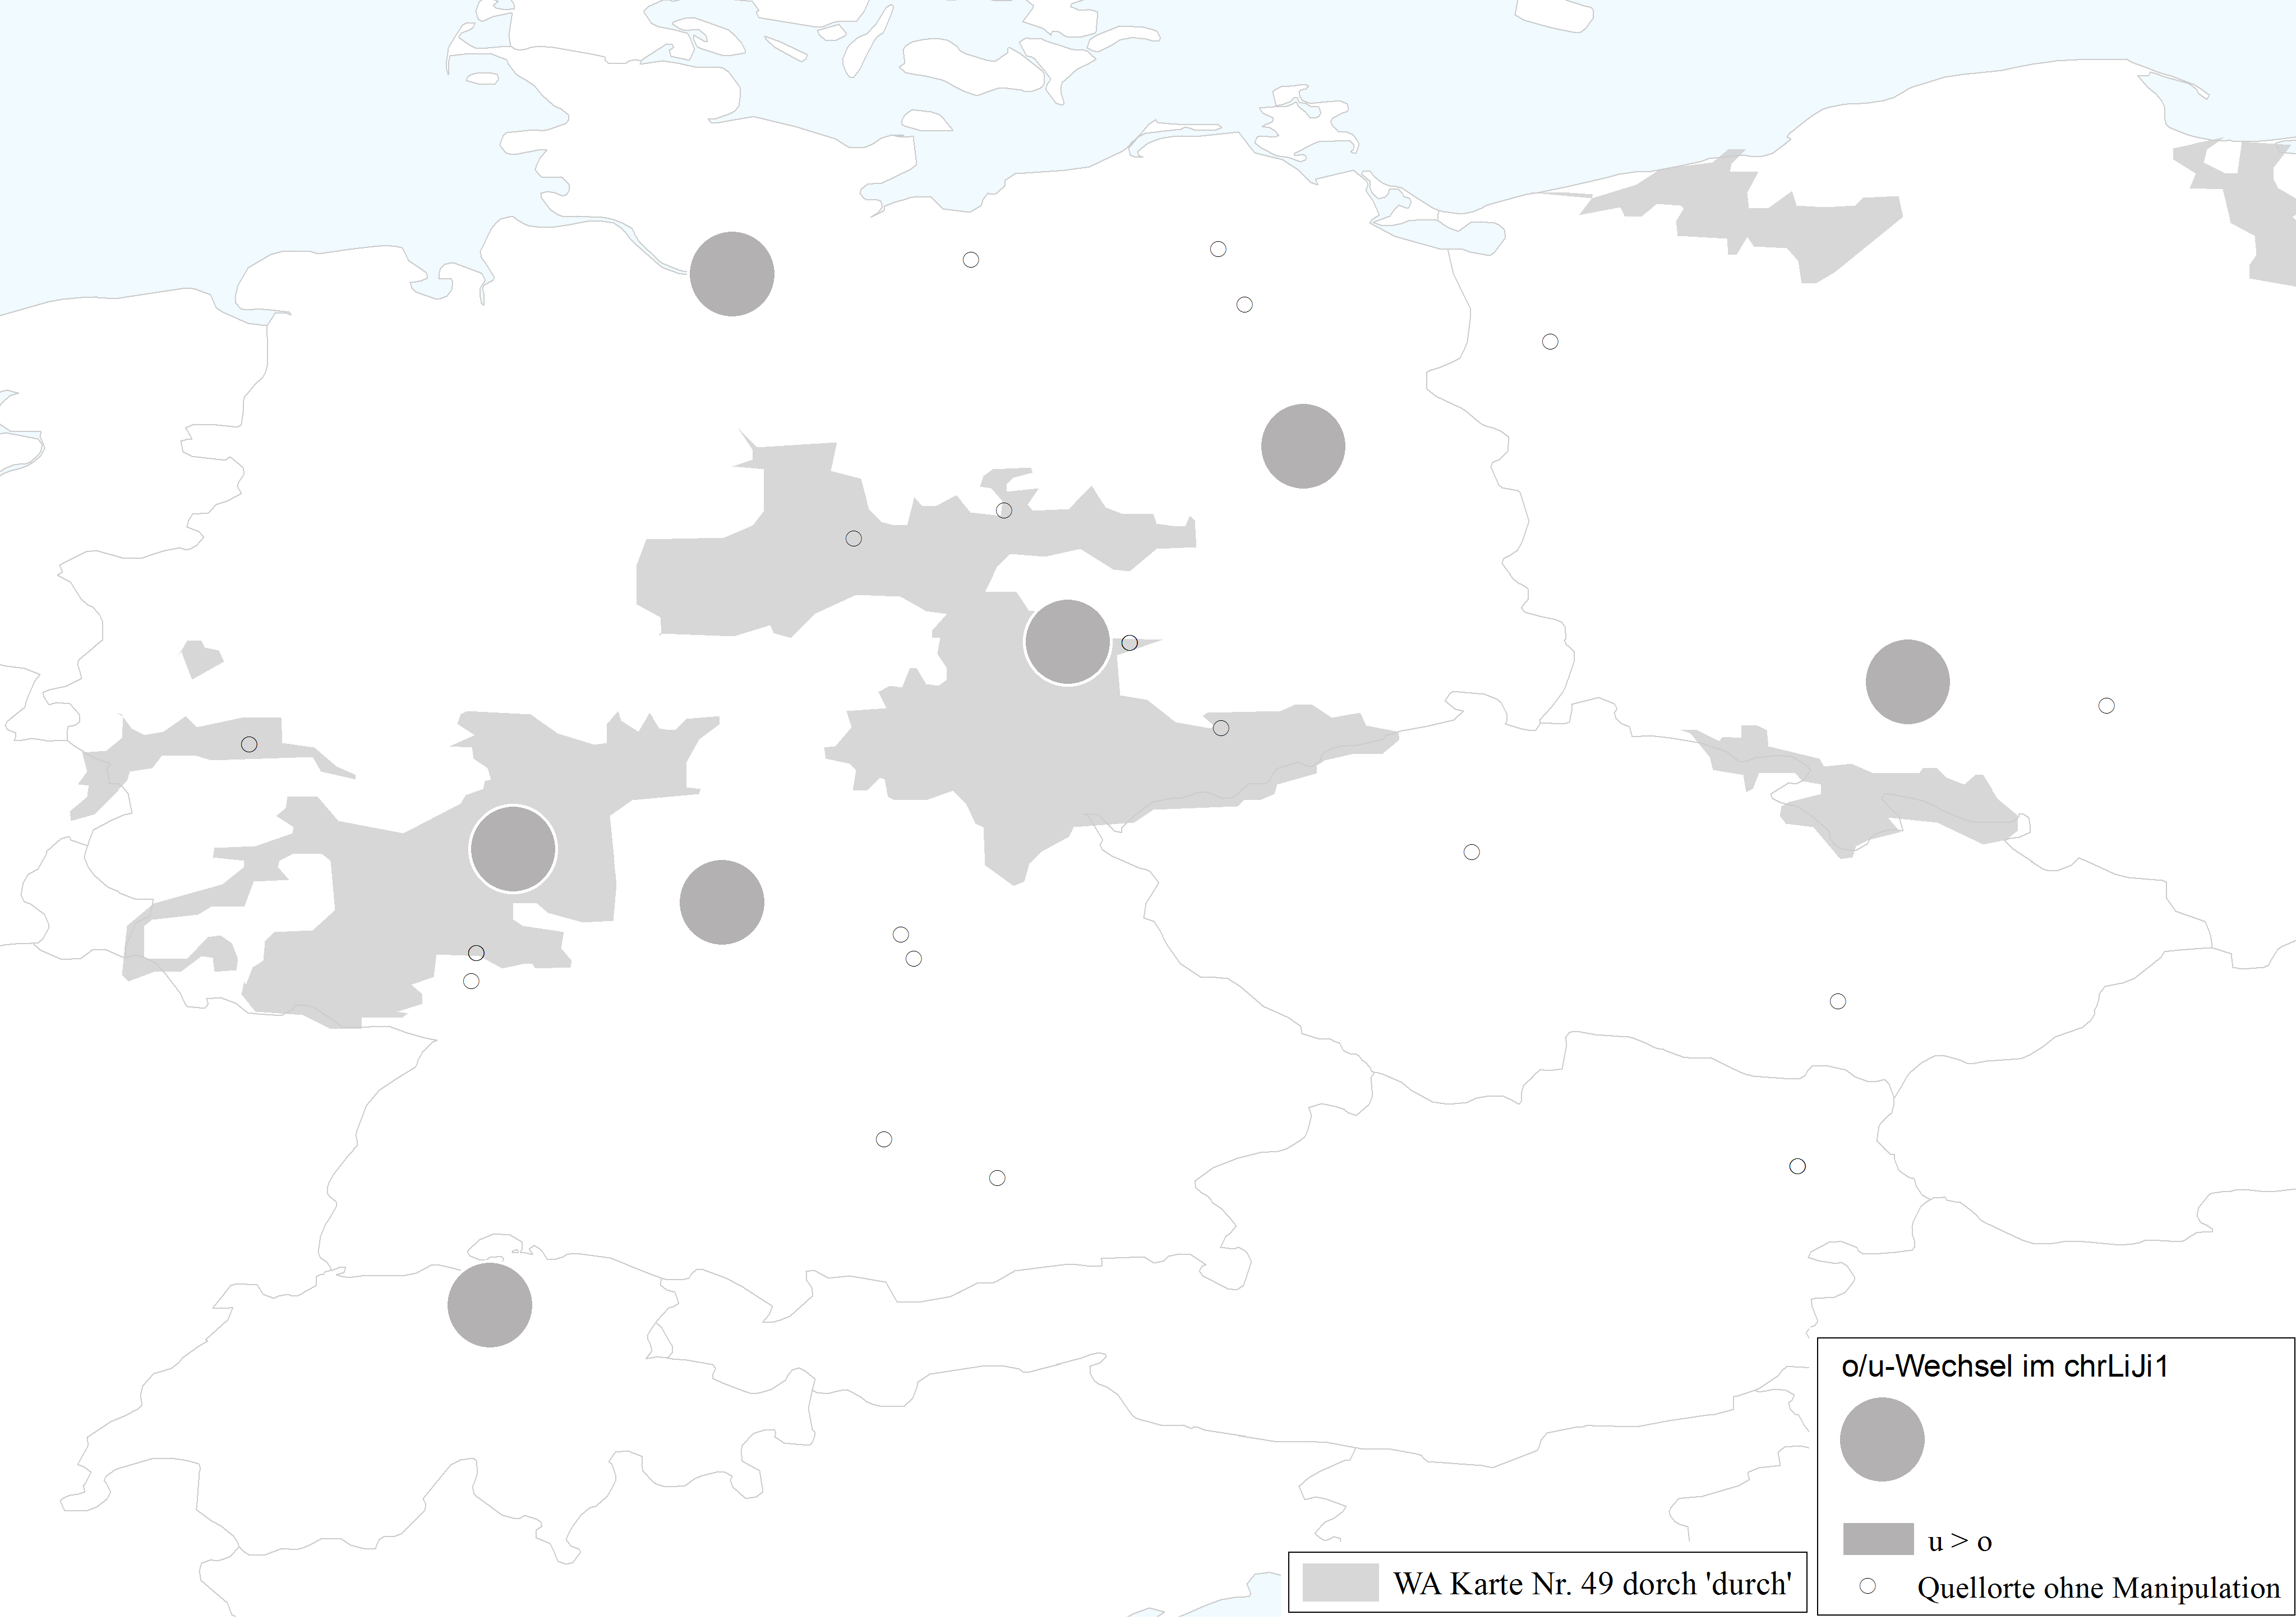
\includegraphics[scale=0.5]{figures/karteuo.png}
		\caption{\label{karteuo} Der Wechsel von /\textit{o}/ > /\textit{u}/ im \hai{chrLiJi1} mit \hai{WA} Karte Nr. 49}
		\end{figure}
\FloatBarrier


Das Phänomen der Senkung von /\textit{u}/ > /\textit{o}/ eignet sich bestens, um den diatopischen Vorteil literaturjiddischer Texte als Sekundärquellen des Westjiddischen zu illustrieren. In der Karte Nr. 35 des \hai{LCAAJ} ist die Situation im Westjiddischen (mit Ausnahme der Situation im \hai{SWJ} Strasbourgs) mit \qu{? no information} versehen (vgl. Abb. \ref{ProtoLCAAJOEWY2}(a)). Die Senkung selbst ist lediglich im \hai{ZOJ} und südlichen \hai{NÜJ} belegt. Vereint man nun die Daten authentischer westjiddischer Quellen (vgl. Bsp. \ref{bspgrob5}–\ref{bspleicht1}) mit den Daten zum \hai{chrLiJi1}, so ergibt sich ein  Kontinuum der Senkung in allen westjiddischen Varietäten bis weit in das ostjiddische Gebiet hinein (vgl. Abb. \ref{ProtoLCAAJOEWY2}(b)).\\
 
 % \begin{center}
 \begin{figure}
\subfloat[\hai{LCAAJ} Karte Nr. 35 \hai{U\textsubscript{1}} before \textit{r}]{\includegraphics[width=1.12\textwidth]{figures/LCAAJ_U1_blanko.png}}

\subfloat[\hai{LCAAJ} Karte Nr. 35 inkl. Belege der Haskala Stücke und \hai{chrLiJi1} Daten]{\includegraphics[width=1.12\textwidth]{figures/LCAAJ_U1_Proto.png}}

\caption{Ergänzung der \hai{LCAAJ}-Daten zur Senkung von /\textit{u}/ > /\textit{o}/ vor <r>}
\label{ProtoLCAAJOEWY2}
\end{figure}
\FloatBarrier
% \end{center}

 
 
 Parallel zur Hebung von /\textit{o}/ > /\textit{u}/ (Unterabschnitt \ref{o_u}) zeigt das \hai{jüdLiJi1} die Senkung von /\textit{u}/ > /\textit{o}/ in den gleichen Quelltexten.\footnote{Diese Quellen sind: \hai{GuS1}, \hai{GuS5}, \hai{GuS10}, \hai{GuS23}, \hai{PAlsleben}, \hai{PBerlin1} u. \hai{PBreslau} (vgl. Fn. \ref{FNo_u}).} 
 
 
  \subsection{Zusammenhang zwischen Hebung und Senkung} \label{ou_uo}

Der durch Hebung und Senkung hervorgerufene komplementäre Wechsel von /\textit{u}/ und /\textit{o}/ wurde im \hai{chrLiJi1} in sieben Quellen durchgeführt.\footnote{In den Quellen \hai{AK} (Zürich, 1948), \hai{GW} (n.a., ca. 1900), \hai{JK} (Breslau, 1810), \hai{MV} (Berlin, 1862), \hai{PA} (Frankfurt, 1834), \hai{SS} (Berlin, 1907) u. \hai{VD} (Frankfurt, 1916).} Im \hai{jüdLiJi1} wurden wie bereits erwähnt (s.\,o.) Hebung und Senkung immer nur parallel durchgeführt. 

Für die Daten des christlichen wie jüdischen \hai{LiJi1} ist allerdings zu bedenken, dass an den Quellorten (Breslau, Berlin, Zürich), an denen die Entwicklungen Hebung und Senkung parallel stattgefunden haben, ein ostjiddischer Einfluss nicht auszuschließen ist (s. Karte in Abb. \ref{karteouuoall}). Dieses Phänomen könnte also auf Interferenzen zum \hai{OJ} im \hai{LiJi} hinweisen. In den deutschen Dialekten fand dieses doppelte Ereignis von Hebung und Senkung nur im Obersächsischen und Moselfränkischen statt (vgl. Abb. \ref{karteouuoall}). Lediglich die Quellen aus Frankfurt a. M. stünden also im Verdacht, eine dialektale Entwicklung aus den deutschen Dialekten zu transportieren. Die Karte zeigt allerdings auch, dass Quellen nur eine der beiden Entwicklungen im \hai{chrLiJi1} zeigen, wo in den deutschen Mundarten beide belegt sind (etwa Mannheim, Leipzig). \\
		
\begin{figure}[h!]
		\centering
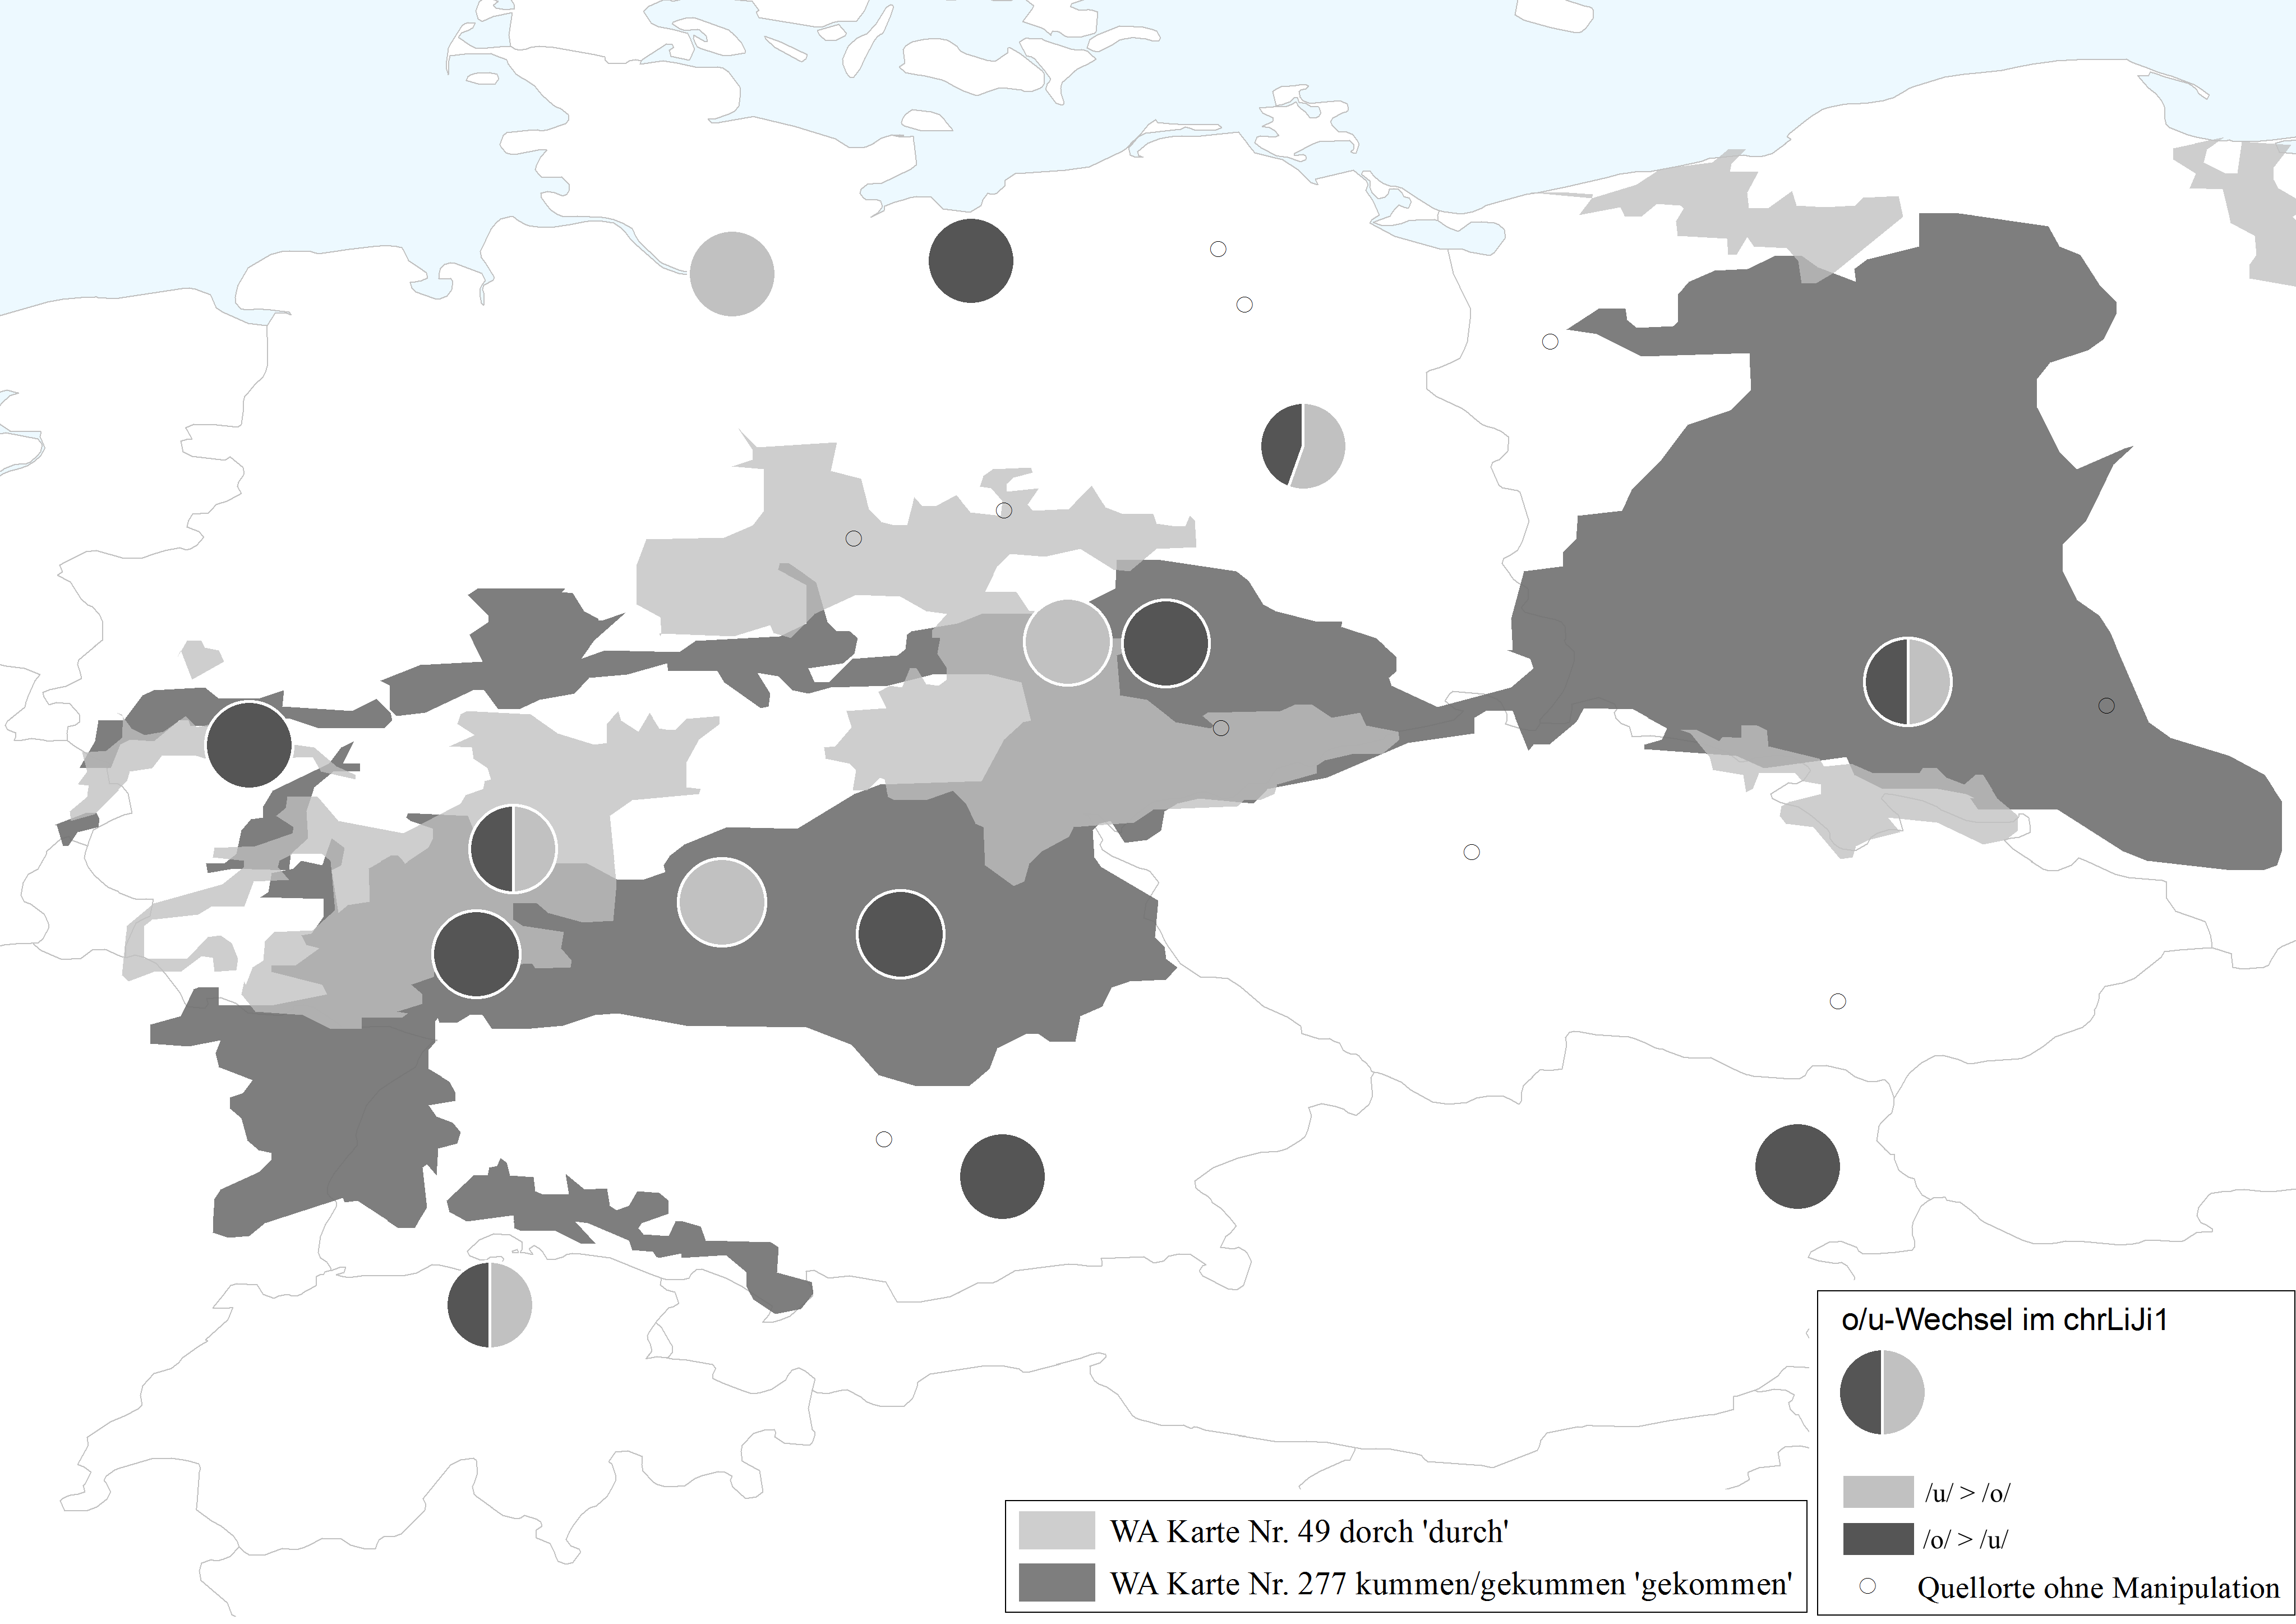
\includegraphics[scale=0.1]{figures/karteouuoall2.png}
		\caption{\label{karteouuoall} Hebung und Senkung von /u/, /o/ im \hai{chrLiJi1} mit \hai{WA} Karten Nr. 277, 49}
		\end{figure}
\FloatBarrier
		

Wie die angeführten Beispiele aus der \qu{Hochzeit zu Grobsdorf} zeigen konnten, ist jedoch nicht auszuschließen, dass dieses Phänomen nicht nur in den ostjiddischen Dialekten, sondern auch in den westjiddischen Varietäten auftritt. Der Umstand, dass in vielen Quellen nur eine Entwicklung (Hebung oder Senkung) stattgefunden hat, lässt immerhin darauf schließen, dass möglicherweise nur eine Regel des komplexen Wechsels der zwei Vokale von den Imitatoren erkannt wurde. Dies lässt an sich noch nicht ausschließen, dass das komplementäre Ereignis im \hai{WJ} nicht stattgefunden hat. \\


 \section{\isi{Palatalisierung} /u/, /u\textlengthmark/ > /y/, /y\textlengthmark/}\label{phonpalat}
 %\noindent 
 Die \isi{Palatalisierung} von /u/, /u\textlengthmark/ > /y/, /y\textlengthmark/ ist ein besonderes Merkmal des Elsässer und ungarischen Jiddisch (vgl. \cite{Birnbaum1934}; \cite[108]{GuggenheimGruenberg1973}; \cite[1027]{Katz1983}; \cite[171f]{Timm1987}; \cite{Hutterer1965}; \cite[83]{Herzog1992}). Es ist anzunehmen, dass /u\textlengthmark/ > /y/ übergangsweise im Zuge der zentralostjiddischen Entwicklung von /u\textlengthmark/ zu /i/ auch im \hai{ZOJ} gegeben war (\cite{Birnbaum1934}; \cite[1029]{Katz1983}). In einem kleinen Teil des nördlichen \hai{SOJ} blieb die \isi{Palatalisierung} von \hai{V51} (\hai{U\textsubscript{1}}) und \hai{V52} (\hai{U\textsubscript{2}}) erhalten (\cite[83]{Herzog1992}). Es besteht zwischen der Elsässer-\isi{Palatalisierung}, die höchst wahrscheinlich durch den \isi{Sprachkontakt} zum Französischen begünstigt war, und der \isi{Palatalisierung} im ungarischen Raum ein wichtiger systematischer Unterschied. Während im südlichen Übergangsjiddisch Ungarns, des Burgenlandes und ggf. auch vereinzelt im \hai{ZOJ} Südposens  (vgl. \cite{FleischerSchaeferErsch}) Lang- und Kurzvokal (\hai{V51}, \hai{V52}, \hai{V53}) palatalisiert wurden, was zu einer Systemverschiebung geführt hat, blieb im Elsässer \ili{Westjiddisch} kurz /u/ erhalten (vgl. \cite{Birnbaum1934}); was heißt, dass hier nur der Langvokal palatalisiert wurde, s. Bsp. \ref{bspY1}--\ref{bspY4}.\\
 
  \eenumsentence{

 \item \textit{tsü}/\textit{ts\={ü}} \sem{zu} (Budapester \hai{SÜJ}; \cite[124]{Hutterer1965}) \label{bspY1}

 
 \item \textit{füks} \sem{Fuchs} (Budapester \hai{SÜJ}; \cite[124]{Hutterer1965})\label{bspY2}
  
  \item \textit{zü} \sem{zu} (Elsässer \hai{SWJ}; \qu{Chateïsim sinn aach Laït} Mulhouse 1929:\,16)\label{bspY3}

 \item \textit{Duckser} (*\textit{Dückser}) \sem{Duckser, Feigling} \\
 (Elsässer \hai{SWJ}; \qu{Chateïsim sinn aach Laït} Mulhouse 1929:\,20)\label{bspY4}
  
  }


 Das Auftreten der \isi{Palatalisierung} im \hai{chrLiJi1} kann damit zum einen auf den jiddischen Dialekten des Elsässer \hai{SWJ}, \hai{SÜJ} und \hai{SOJ} beruhen, zum anderen aber könnte die \isi{Palatalisierung} tatsächlich auch in manchen westjiddischen Dialekten stattgefunden haben oder aber die Belege stellen \quein{Fehler} dar. 
 
 In 13 Texten lassen sich Belege für die \isi{Palatalisierung} finden. Die diachrone Verteilung der Belege zeigt, dass sich diese  in den zwischen 1805 und 1825 erschienenen Quellen besonders häuft (vgl. Abb. \ref{palat}). Aber bereits zwei ältere Quellen von 1770 und 1773 zeigen dieses Phänomen. In der zweiten Hälfte des 19. Jahrhunderts finden wir sie vereinzelt bis ins 20. Jahrhundert hinein.\\
 
  %%%palat Diagramm%\begin{flushleft}	
\begin{figure}[h!]
	\begin{tikzpicture}
		\begin{axis}[only marks, width=0.82\textwidth,height=0.2\textheight,
		legend style={at={(1,1)},xshift=+0.2cm, yshift=-0.6cm,anchor=north west,nodes=left},
			%title={Funktionstypen des sp\"aten Westjiddisch},
			xtick={1700, 1725, 1750, 1775, 1800, 1825, 1850, 1875, 1900, 1925, 1950, 1975}, ytick=\empty,
			x tick label style={/pgf/number format/1000 sep=}, 
			y tick label style={/pgf/number format/1000 sep=},
			%extra y ticks={456.1, 1022.4},
			%extra y tick labels={{456,1},{1022,4}},
			extra y tick style={grid=major,
				tick label style={, ,}},
				ymin=0.7,
				ymax=2.9,
			ylabel={Phänomenbelege},
			enlarge x limits=0.03]	
	
			
\addplot [mark=*, black] table [x=jahr, y=phaen] {figures/palat.txt}; %2

\addplot [mark=o, black] table [x=jahr, y=no] {figures/palat_no.txt}; %1.5

			% Andere Formen a={mark=square*,blue},% b={mark=triangle*,red},% c={mark=o,draw=black}}
						\legend{<u> als <ü>, unmanipuliert} %macht Legende
		\end{axis}
	\end{tikzpicture}
	\caption{\isi{Palatalisierung} von /\textit{u}(\textlengthmark)/ > /\textit{y}(\textlengthmark)/ im \hai{chrLiJi1}}
	\label{palat}	
\end{figure}
\FloatBarrier
 
 Neun der elf Quellen zeigen die \isi{Palatalisierung} sowohl beim Lang- als auch beim Kurzvokal. Die übrigen vier Quellen haben nur an einem Lexem palatalisiert und zeigen damit auch nur bei Kurzvokal (\hai{JK} Breslau, 1810 u. \hai{TH} Merseburg, 1820) oder Langvokal (\hai{AO} Wien, 1770 u. \hai{SV} München, 1890) dieses Phänomen. aufgrund der schmalen Datengrundlage lässt sich hier nicht feststellen, ob die Verfasser gezielt nur am Lang- bzw. Kurzvokal <ü> gesetzt haben, was prinzipiell in den Quellorten nicht anzunehmen ist. 
 
 Besonders auffällig gestalten sich die Belege zur \isi{Palatalisierung} in ihrer räumlichen Verteilung (s. Abb. \ref{kartepalat}). Sie tritt ausschließlich in östlichen Quelltexten auf und ganz besonders in Texten aus Berlin und Wien. Hier ist ein Einfluss des Ostjiddischen und südlichen Übergangsjiddischen nicht auszuschließen. Unter Umständen könnten die Daten aus dem \hai{chrLiJi1} tatsächlich ein Hinweis dafür sein, dass die \isi{Palatalisierung} tatsächlich weiter ins östl. \hai{WJ} hinein gestreut hat als bisher angenommen. Zu den entsprechenden Regionen fehlen jedoch noch vergleichbare Daten aus den westjiddischen Dialekten. 
 
 Eine Beeinflussung des \hai{chrLiJi1} durch die koterritorialen deutschen Dialekte ist zumindest bei den nordöstlichen Quellen (und damit auch den Quellen Berlins) nicht auszuschließen. Die Vergleichskarte des \hai{WA} zeigt, dass wir die \isi{Palatalisierung} besonders im Niederdeutschen finden.\footnote{Was die \hai{WA}-Karte nicht abdeckt, ist die konsequent durchgeführte \isi{Palatalisierung} im Elsässer Nieder\ili{alemannisch} und im Höchst\ili{alemannisch} (\cite[208–210]{Schirmunski1962}; \cite[831]{Wiesinger1983a}; \citeyear[1052]{Wiesinger1983b}).}

  \begin{figure}[h!]
		\centering
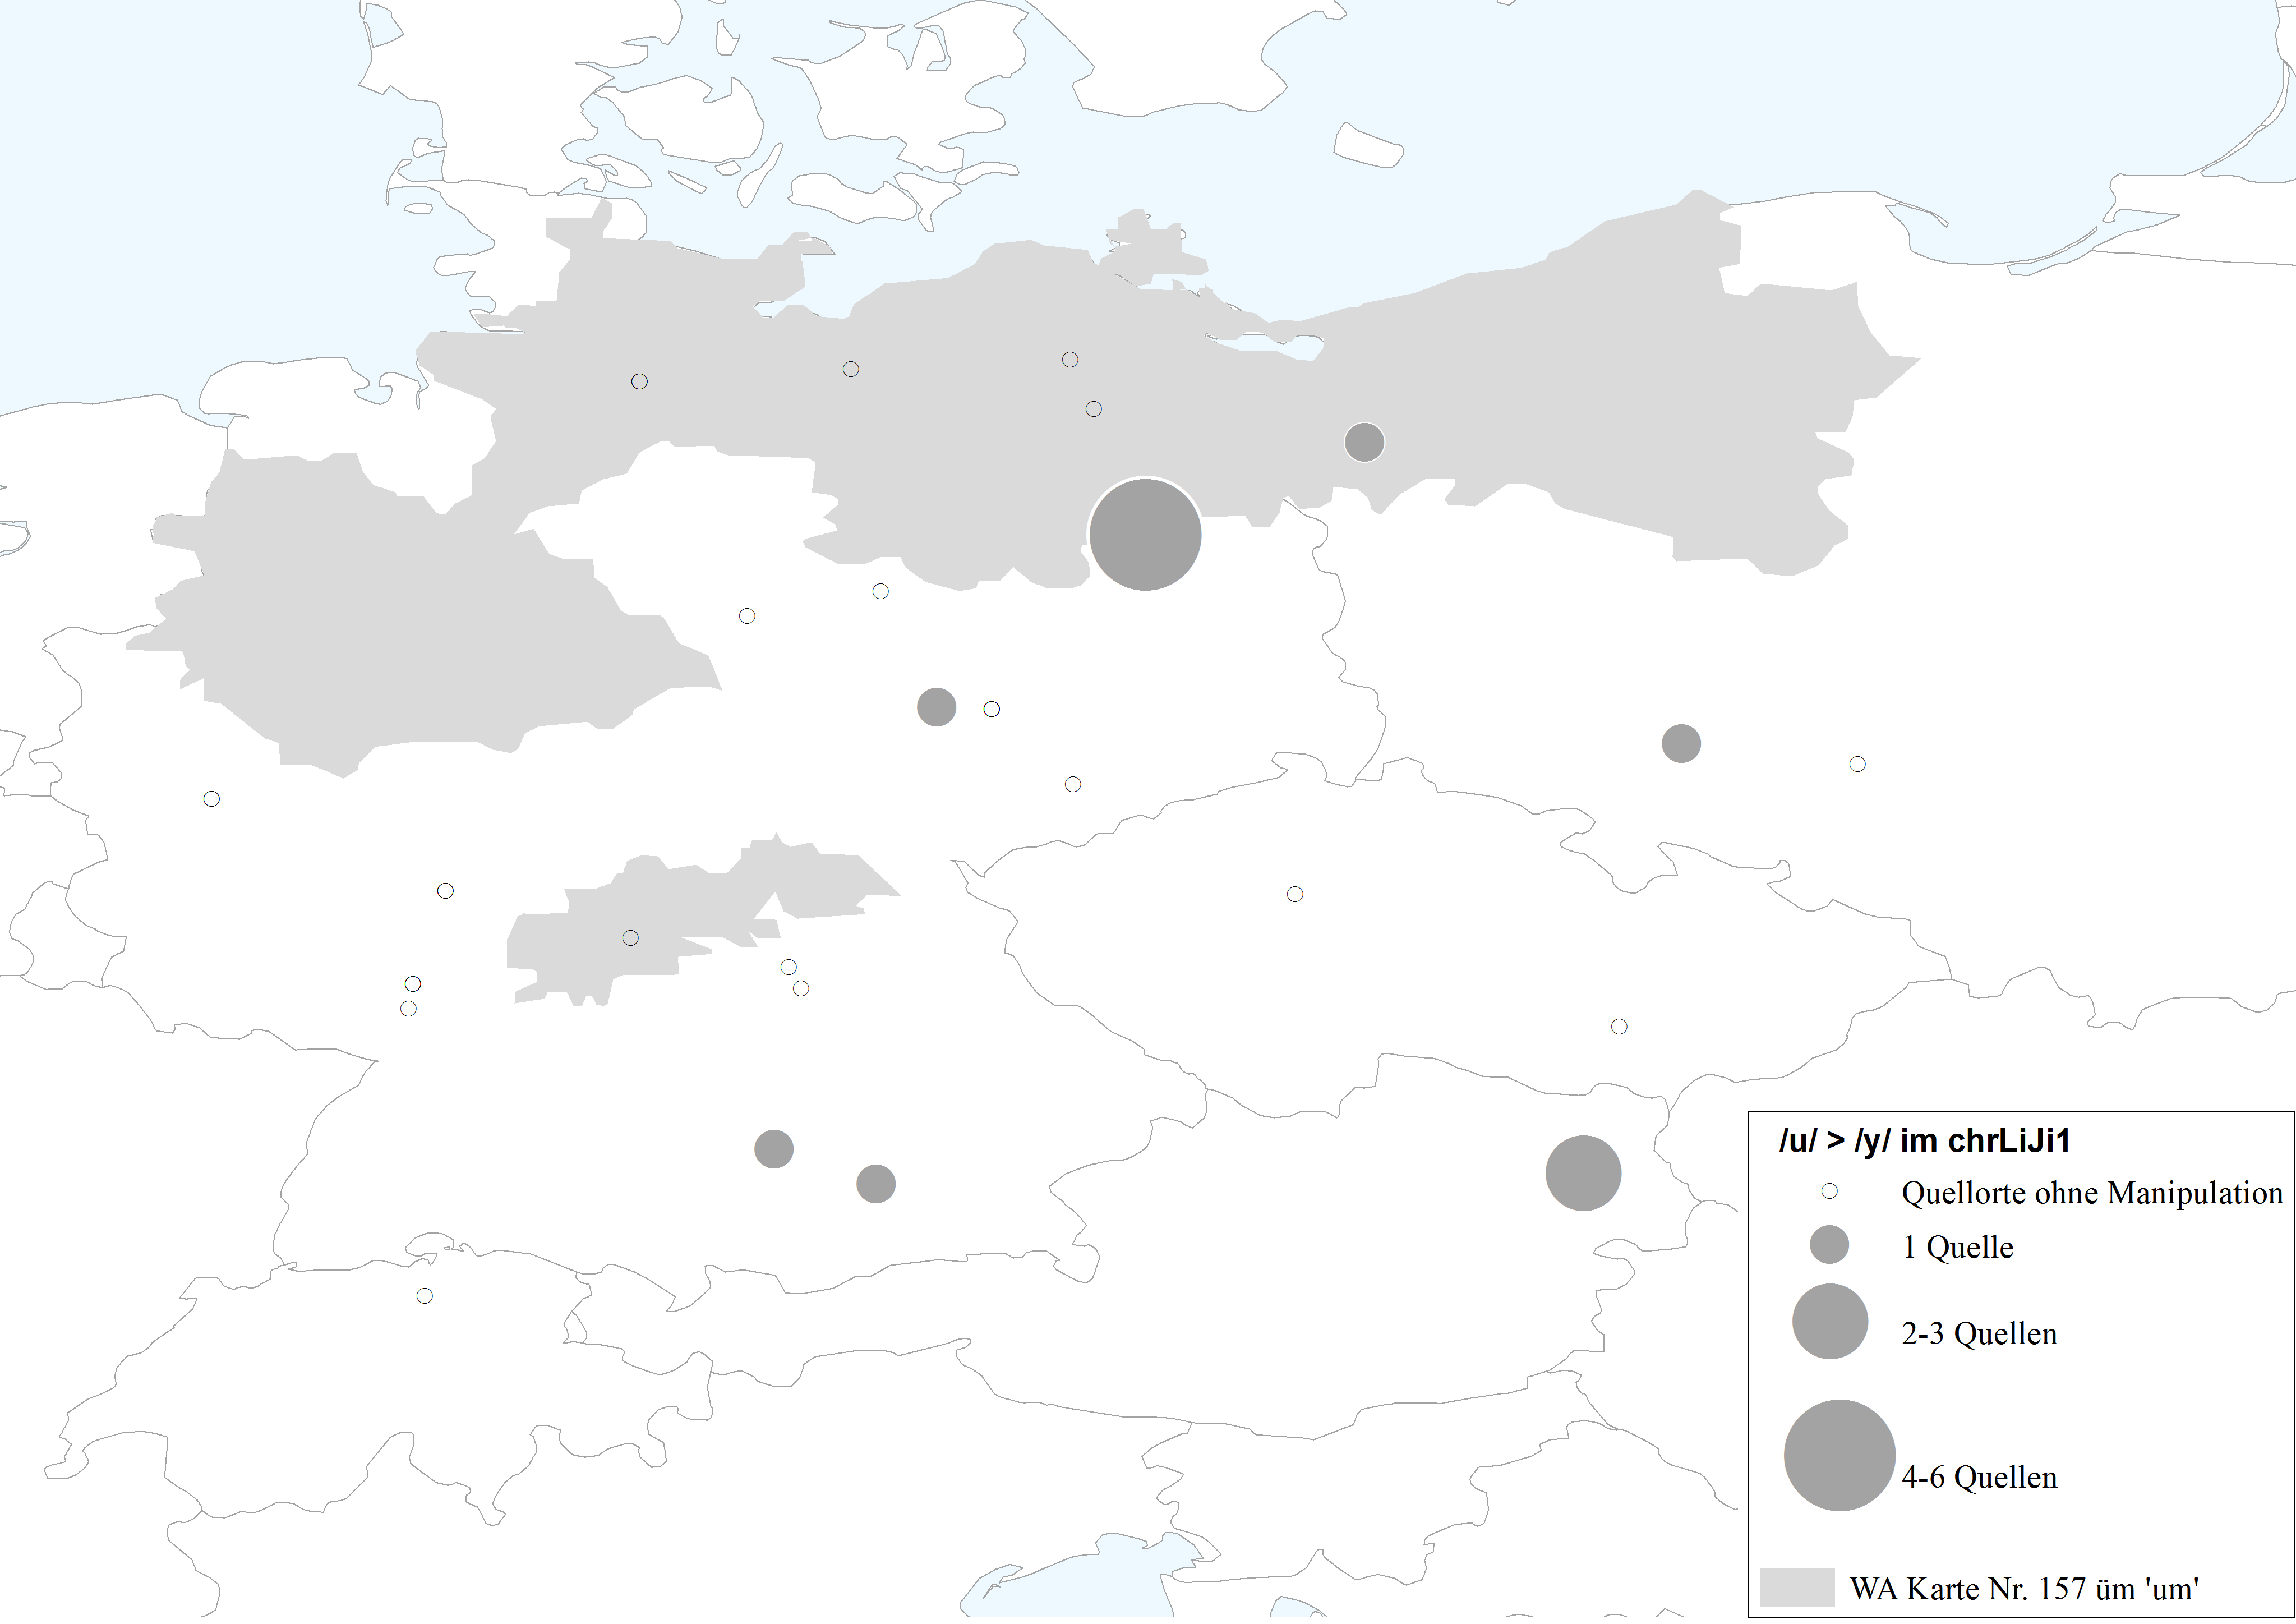
\includegraphics[scale=0.1]{figures/palatkarte2.png}
		\caption{\label{kartepalat} \isi{Palatalisierung} von /\textit{u}(\textlengthmark)/ > /\textit{y}(\textlengthmark)/ im \hai{chrLiJi1} mit \hai{WA} Karte Nr. 157}
		\end{figure}
\FloatBarrier
 
 
 Aufgrund fehlender Daten aus den westjiddischen Mundarten und insbesondere in Anbetracht der auffälligen geographischen Verteilung ist nicht mit Bestimmtheit zu entscheiden, ob wir es bei diesem Phänomen mit einer \quein{fehlerhaften} \isi{Imitation} des Jiddischen zu tun haben oder ob es an den entsprechenden Orten im Jiddischen tatsächlich präsent war, selbst wenn diese Präsenz nur durch angesiedelte Sprecher des \hai{SÜJ} oder \hai{SOJ} gegeben war. 
 
Als eine Bestätigung für die Hypothese, dass die \isi{Palatalisierung} im östlichen \hai{WJ} Einzug gefunden hatte, könnten Belege derselben im \hai{jüdLiJi1} verstanden werden. Das \hai{jüdLiJi1}, dessen Quellen aus eben den östlichen Regionen stammen, in denen wir die \isi{Palatalisierung} im \hai{chrLiJi1} nachweisen konnten, zeigt dieses Phänomen in fünf Quellen.\footnote{Die da wären: \hai{GuS1}, \hai{GuS23}, \hai{PAlsleben}, \hai{PBerlin2} und \hai{PDebrecen}.} Im Fall der ungarischen Quelle \hai{PDebrecen} überrascht dies nicht, da wir hier eben jene Entwicklung aus dem Jiddischen kennen (vgl. \cite{Hutterer1965}; \cite[83]{Herzog1992}). Anders ist es im Fall der sächsischen Quelle \hai{PAlsleben}, von wo die \isi{Palatalisierung}, von den oben angeführten Texten aus dem \hai{chrLiJi1}, von Leipzig abgesehen (Abb. \ref{palat}), bislang nicht bekannt war. \\
 

 
    \section{Entrundungen (nhd. <ü>, <ö> > <i>, <e>)}\label{entrundung}
 %\noindent
Die hier als \isi{Entrundung} bezeichnete Entwicklung von mhd. \textit{u}, \textit{ü} zu /i/ und die weitergeführte Senkung zu /e/ fand z.\,T. bereits im Mitteljiddischen statt (\cite[173f, 209–213]{Timm1987}). Der diachrone Ablauf des gesamten Prozesses, der im modernen \hai{OJ} zum totalen Abbau der Umlaute von /u/ führte und auf den Abbau der Umlaute von /a/ und /o/ übergriff, ist jedoch noch ungeklärt. Anzunehmen ist, dass die \isi{Entrundung} in einzelnen Schüben einzelne Lexeme betraf (\textit{lexical diffusion}). So ist im modernen \hai{OJ} mhd. \textit{u}, \textit{ü} zwar zumeist zu /i/ entrundet worden, z.\,B. in Bsp. \ref{bspentr1}–\ref{bspentr4}. Zum Teil hat die \isi{Entrundung} aber auch zu einer weiteren Senkung geführt, wie etwa in Bsp. \ref{bspentr5}–\ref{bspentr7} oder es blieb sogar der mhd. ungerundete Vokal erhalten, Bsp. \ref{bspentr8}–\ref{bspentr9}. Die \isi{Entrundung} hat so auch im späten \hai{WJ} gewirkt, Bsp. \ref{bspgrob12}–\ref{bspgrob11}; bewirkte allerdings z.\,T. andere Folgeprozesse als im Standardostjiddischen, vgl. \ref{bspentr8} vs. \ref{bspgrob14}. Die Präsenz der \isi{Entrundung} von mhd. \textit{u}, \textit{ü} im \hai{LiJi} mag daher auf jiddische Sprachrealitäten fußen.\\
 
 
 
 \eenumsentence{
	\item oj. \RL{גליקלעך} \textit{gliklekh} \sem{glücklich} < mhd. \textit{gelücke}, \textit{glücke} \parencite[Bd. 1, Sp. 829]{Lexer1992} \label{bspentr1} 
	
	
	\item oj. \RL{טיר} \textit{tir} \sem{Tür} < mhd. \textit{Tür} \parencite[Bd. 2, Sp. 1579]{Lexer1992} \label{bspentr2}
	
	\item oj. \RL{קענען} \textit{kenen} \sem{können} < mhd. \textit{künnen}, \textit{kunnen} \parencite[Bd. 1, Sp. 1778]{Lexer1992} \label{bspentr3}
	
	\item oj.\RL{מעגן} \textit{megen} \sem{mögen} < mhd. \textit{mügen}, \textit{mugen} \parencite[Bd. 1, Sp. 2218]{Lexer1992} \label{bspentr4}
	
	\item oj. \RL{פֿא\makebox(-1.5,-7.5)[r]{\libertineGlyph{uni207B}}ר}
 \textit{far} \sem{für} < mhd. \textit{vür}, \textit{vüre} \parencite[Bd. 3, Sp. 583–585]{Lexer1992} \label{bspentr5}
 
 	\item oj. \RL{דא\makebox(-1.5,-7.5)[r]{\libertineGlyph{uni207B}}רפֿן} \textit{darfn} \sem{dürfen, brauchen} < mhd. \textit{dürfen}, \textit{durfen} \parencite[Bd. 1, Sp. 494]{Lexer1992} \label{bspentr6}
 
	 \item oj. \RL{דא\makebox(-1.5,-7.5)[r]{\libertineGlyph{uni207B}}ר} \textit{dar} \sem{dürr} < mhd. \textit{dürre}, \textit{durre} \parencite[Bd. 1, Sp. 497]{Lexer1992} \label{bspentr7}

	\item oj. \RL{מוזן} \textit{muzn} \sem{müssen} < mhd. \textit{müeʒen} (md. \textit{mûʒen} \textit{môʒen}) \parencite[Bd. 1, Sp. 2217]{Lexer1992}\label{bspentr8}
	
	\item  oj. \RL{קושן} \textit{kushn} \sem{küssen} < mhd. \textit{küssen} (md. \textit{kussen}) \parencite[Bd. 1, Sp. 1801]{Lexer1992}\label{bspentr9} 
	
	\item \RL{אונגליק} \textit{unglick} \sem{Unglück} (\qu{Die Hochzeit zu Grobsdorf} 1822:\,9)
\label{bspgrob12}

	\item \RL{מיזע} \textit{mizn} \sem{müssen} (\qu{Die Hochzeit zu Grobsdorf} 1822:\,u.\,a. 55)
\label{bspgrob14}

	\item \RL{קעננע} \textit{kenne} \sem{können} (\qu{Die Hochzeit zu Grobsdorf} 1822:\,10)
\label{bspgrob13}

	
	\item \RL{פאר} \textit{far} \sem{für} (\qu{Die Hochzeit zu Grobsdorf} 1822:\, u.\,a.19)
\label{bspgrob11} 
 

}\label{entrundungbsp}
 
 
Die jiddische Entwicklung findet allerdings ihre Parallelen in den deutschen Dialekten, wo die \isi{Entrundung} von mhd. \textit{u}, \textit{ü} und \textit{o}, \textit{ö} wie auch der Diphthonge \textit{öu}, \textit{üe} ab mittelhochdeutscher Zeit einsetzt und letzten Endes beinahe überall in unterschiedlicher Stärke wirksam wird, jedoch nirgends so konsequent, wie im \hai{OJ}. Resistent blieben allein der Norden des Ripuarischen, das Ostfränkische inkl. des angrenzenden Thüringischen, das Schweizer, Bodensee- und Vorarlberger Alemannisch (mit Ausnahme des südlichen Höchstalemannischen) (\cite[204–208]{Schirmunski1962}). Unter Umständen können damit auch die deutschen Dialekte in das \hai{LiJi} hineingespielt haben.
 
 Im \hai{chrLiJi1} überwiegt deutlich die \isi{Entrundung} von <ü> > <i> (14 Quellen); Entrundungen von <ü> und <ö> zu <e> finden sich jeweils in 10 Quellen. Die Entrundungen von nhd. <ö> im \hai{chrLiJi1} beruhen zum einen auf einem Erhalt des mhd. Vokals \textit{ë}, z.\,B. in \textit{Lewenthaler} \sem{Löwenthaler} (\hai{FM} Leipzig, 1852:\,21, 28, 29, 31) < mhd. \textit{lëwe} \parencite[Bd. 1, Sp. 1893]{Lexer1992} oder stellen, was weitaus häufiger der Fall ist, eine Senkung von palatalisiertem germ. \textit{u} dar, etwa in \textit{mechten} \sem{möchten} (\hai{GW} n.a., ca. 1900:\,3, 4, 10; \hai{SS} Berlin, 1907:\,18; \hai{SV} München, 1890:\,1) < mhd. \textit{mügen, mugen} (ahd. \textit{mugan}) \parencite[Bd. 1, Sp. 2218]{Lexer1992}. Die \quein{einfache} \isi{Entrundung}, sprich eine nicht weiter gesenkte Form, liegt nur in einem Beleg vor: \textit{kinne} \sem{können} (\hai{PG} Speyer, 1835:\,34) < mhd. \textit{kunnen, künnen} \parencite[Bd. 1, Sp. 1778]{Lexer1992}. Diese Quelle ist auf den Ortspunkt Speyer zurückzuführen, wo im örtlichen deutschen Dialekt eben jene Form gebräuchlich ist (vgl. \hai{PfWB} \citeyear[Bd. 4, Sp. 445]{PfaelzWB}). Eine Interferenz aus dem Deutschen lässt sich demnach nicht ausschließen.
 
Zehn Korpustexte weisen mehrere Entrundungsstrategien auf, wie etwa <ö> > <e> und <ü> > <i>. Sie bleiben dabei aber konsequent lexemgebunden, d.\,h. wenn in einem Lexem nhd. <ü> als <i> gesetzt ist, dann wird dies konsequent beibehalten. In neun Quellen findet sich lediglich jeweils eine der vier möglichen Entrundungen. 

 Wir sehen im Histogramm (Abb. \ref{entrliji}), dass Entrundungen von <ü> und <ö> (< mhd. \textit{ü}) erst zu einem späteren Stadium des \hai{chrLiJi1} auftritt. Ab den 1820er Jahren wird dieses Phänomen populär. In acht Quellen tritt die \isi{Entrundung} von <ü> neben der von <ö> auf.\footnote{Diese Quellen sind \hai{AK} (Zürich, 1948), \hai{GW} (n.a., ca. 1900), \hai{JP} (Altona, 1867), \hai{PA} (Frankfurt, 1834), \hai{SS} (Berlin, 1907), \hai{SV} (München, 1890), \hai{TH} (Merseburg, 1820) u. \hai{VD} (Frankfurt, 1916).}
 
 %%%\isi{Entrundung}%\begin{flushleft}	
\begin{figure}[h!]
	\begin{tikzpicture}
		\begin{axis}[only marks, width=0.82\textwidth,height=0.2\textheight,
		legend style={at={(1,1)},xshift=+0.2cm, yshift=0cm,anchor=north west,nodes=left},
			%title={Funktionstypen des sp\"aten Westjiddisch},
			xtick={1700, 1725, 1750, 1775, 1800, 1825, 1850, 1875, 1900, 1925, 1950, 1975}, ytick=\empty,
			x tick label style={/pgf/number format/1000 sep=}, 
			y tick label style={/pgf/number format/1000 sep=},
			%extra y ticks={456.1, 1022.4},
			%extra y tick labels={{456,1},{1022,4}},
			extra y tick style={grid=major,
				tick label style={, ,}},
				ymin=0.4,
				ymax=3.1,
			ylabel={Phänomenbelege},
			enlarge x limits=0.03]	
	
			
			\addplot [mark=*, black] table [x=jahr, y=ue_i] {figures/ue_i.txt}; %2.6
			\addplot [mark=*, gray] table [x=jahr, y=ue_e] {figures/ue_e.txt}; %2.3
			\addplot [mark=square*, draw=black] table [x=jahr, y=oe_e] {figures/oe_e.txt}; % 1.7
			\addplot [mark=square*,gray] table [x=jahr, y=oe_i] {figures/oe_i.txt}; %1.4
			\addplot [mark=o,black] table [x=jahr, y=no] {figures/oe_i_no.txt}; %1.1



			% Andere Formen a={mark=square*,blue},% b={mark=triangle*,red},% c={mark=o,draw=black}}
						\legend{<ü> als <i> , <ü> als <i>, <ö> als <e>, <ö> als <i>, unmanipuliert} %macht Legende
		\end{axis}
	\end{tikzpicture}
	\caption{Entrundungen im \hai{chrLiJi1}}
	\label{entrliji}	
\end{figure}
\FloatBarrier




Ein verhältnismäßig häufig entrundetes Lexem stellt \sem{für} > \textit{fer} dar. Es findet sich in fünf Quellen.\footnote{Die Quellen mit der \isi{Entrundung} von \sem{für} sind  \hai{AJ} (Berlin, 1825):\,2; \hai{GW} (n.a., ca. 1900):\,3,4,5; \hai{JK} (Breslau, 1810):\,13,20,42; \hai{PA} (Frankfurt, 1834):\,5; \hai{SV} (München, 1890):\,1,4,8,9.} Aus diesem Grund wird für die Vergleichskarte (Abb. \ref{karteentrundung}) die \hai{WA}-Karte zu diesem Lexem herangezogen. Zuzüglich wurden Streubelege , d.\,h. Belege die in der Kartierung Wenkers nicht unter Areale zusammengefasst wurden, zur \isi{Entrundung} von <i> am Lexem \sem{Stückchen} zu Arealen zusammengefasst und in die Kartierung in Abbildung \ref{karteentrundung} aufgenommen.\footnote{Wie in der Karte in Abb. \ref{karteentrundung} zu sehen ist, sind diese Streubelege deutlich arealbildend. Der Umstand, dass die Wenkerkarten dies nicht erfassen, zeigt um ein weiteres, wie problematisch die Kartierungsmethoden Wenkers sind.} Vergleichskarten zur \isi{Entrundung} von nhd. <ö> konnten leider keine (brauchbaren)\footnote{Es gibt zwar eine halbe (!) Karte zu den Formen von \sem{könnt} (\hai{WA} Karte Nr. 384), doch diese deckt nur den nördl. Teil des Erhebungsgebiets ab.} herangezogen werden. Da die \isi{Entrundung} im beinahe gesamten deutschen Sprachgebiet gewirkt hat, sind die hier ausgewählten Lexeme und die sich daraus ergebenden Areale lediglich als Richtwert zu nehmen. Das sich damit ergebende Raumbild der \isi{Entrundung} im \hai{chrLiJi1} zeigt keine besonderen Auffälligkeiten, sei aber der Vollständigkeit halber hier angeführt (s. Abb. \ref{karteentrundung}). \\


 \begin{figure}[h!]
		\centering
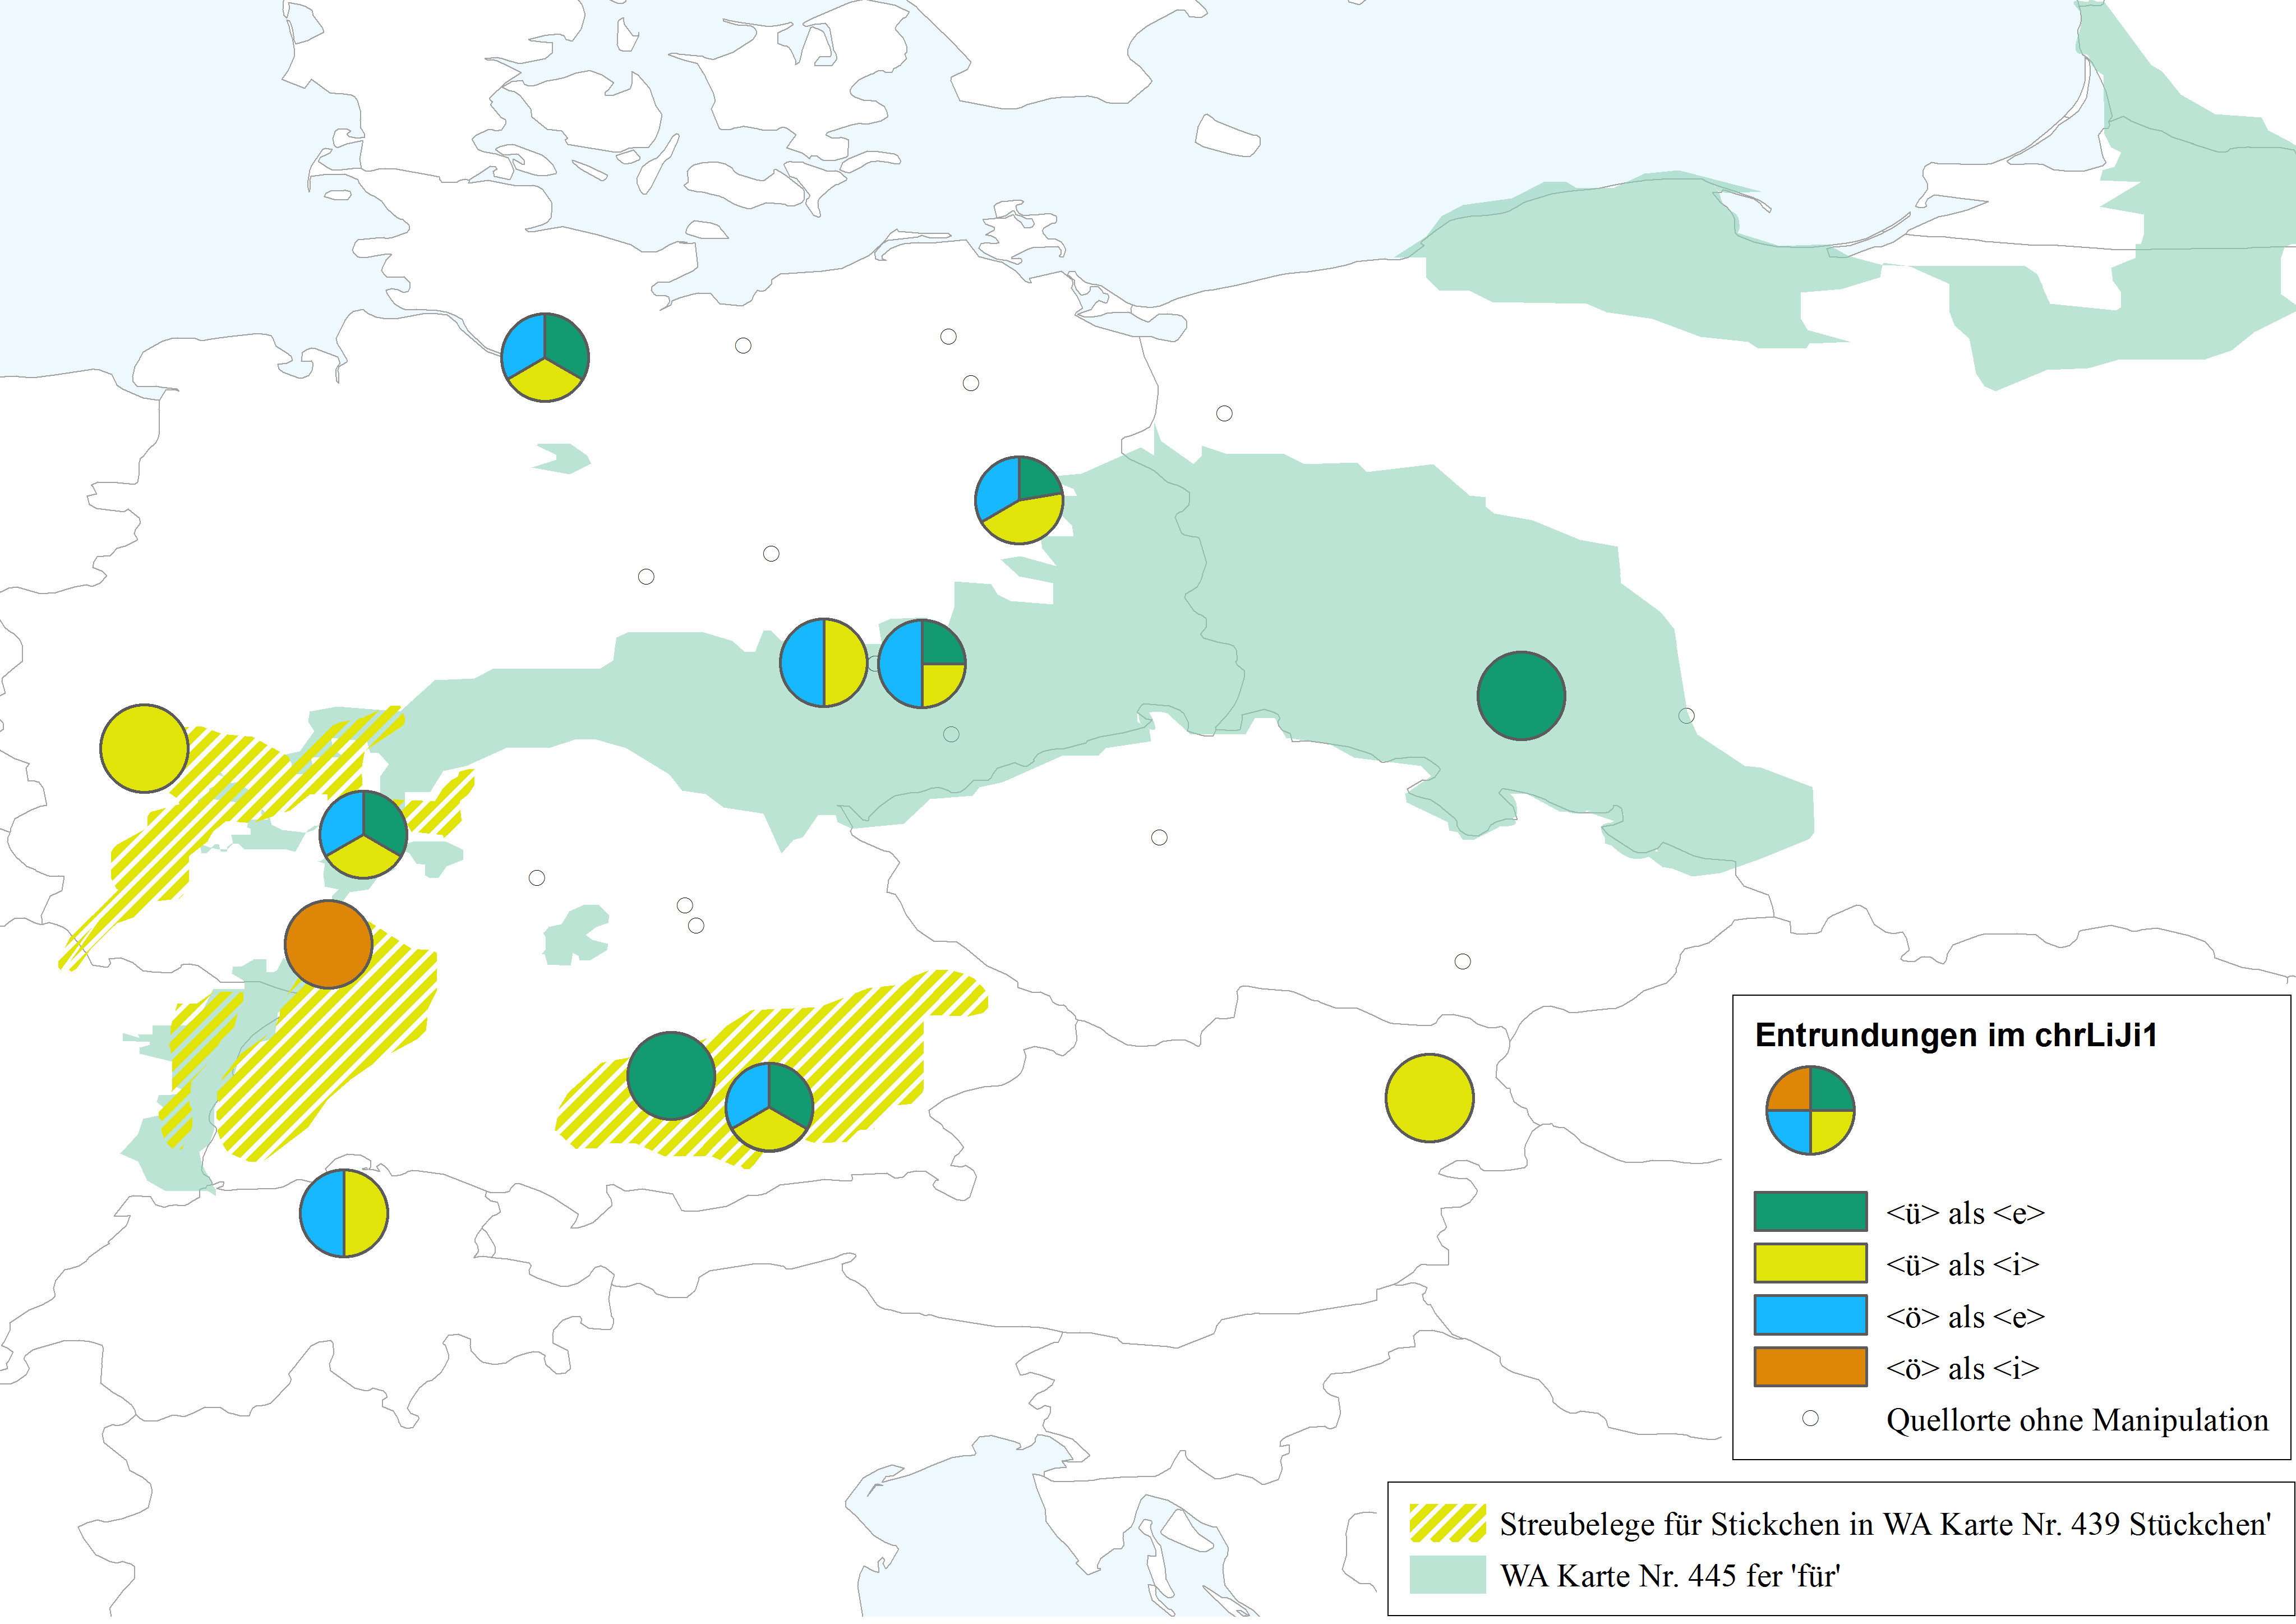
\includegraphics[scale=0.1]{figures/entrundung_karte2.png}
		\caption{\label{karteentrundung} Entrundungen im \hai{chrLiJi1} mit \hai{WA} Karten Nr. 439 u. 445}
		\end{figure}
\FloatBarrier


Das Subkorpus zum \hai{jüdLiJi1} zeigt in sechs Quellen die \isi{Entrundung} von <ü> zu <i>\footnote{Dies ist in den Quellen \hai{GuS10}, \hai{GuS23}, \hai{PAlsleben}, \hai{PBerlin2}, \hai{PBreslau} u. \hai{PDebrecen} der Fall.} und in fünf Quellen die von <ü> zu <e>\footnote{Gegeben in den Quellen \hai{GuS1}, \hai{GuS23}, \hai{PAlsleben}, \hai{PBerlin1} u. \hai{PBerlin2}.}. <ö> zu <e> findet sich in vier Quellen\footnote{In den Quellen \hai{GuS5}, \hai{GuS15}, \hai{PAlsleben} u. \hai{PDebrecen}.} und <ö> zu <i> in lediglich zwei Quellen der \hai{GuS}.\footnote{Zu finden in \hai{GuS1} u. \hai{GuS15}. In beiden Fällen findet sich lediglich das Lexem \sem{gönnen} zu \textit{ginnt} entrundet.} Auf lexikalischer Ebene finden sich zum \hai{chrLiJi1} marginale Unterschiede bei der Wahl der Lexeme, an denen entrundet wird. Ein direkter Unterschied zeigt die \isi{Entrundung} am Lexem \sem{für}. Während dieses im \hai{chrLiJi1} besonders zu \textit{fer} entrundet (s.\,o.), palatalisiert und gesenkt wurde, ist es im \hai{jüdLiJi1} der \hai{GuS} gesenkt als \textit{for} (\hai{GuS1}:\,5; \hai{GuS10}:\,5,6,7), in der ungarischen Quelle \hai{PDebrecen} als \textit{far} (\hai{PDebrecen}:\,5,6) und nur in einem Fall als \textit{fer} belegt (\hai{PAlsleben}:\,5).


Das generelle Bild zur \isi{Entrundung} zeigt, dass dies kein besonders häufiges Phänomen des \hai{LiJi} ist. Die Tokenzahl zu diesem Phänomen ist auffällig gering. In der Regel wurden nur wenige, einzelne Lexeme einer \isi{Entrundung} unterzogen. Eine wirklich systematische Umsetzung der \isi{Entrundung} findet sich ausschließlich im Korpustext \hai{WWR}. Dass die \isi{Entrundung} nicht weiter als Mittel zur \isi{Imitation} des Jiddischen eingesetzt wurde, verwundert besonders, da das Fehlen der Umlaute von /a/, /u/ und /o/ im Jiddischen einen besonders starken Kontrast zum Schriftdeutschen darstellt und leicht als eine Regel wie etwa [{\textit{<ä>, <ü>, <ö> zu <e>}] umgesetzt werden könnte. Solche Hyperkorrekturen des Phänomens findet sich auch vereinzelt.}
Die Autoren des \hai{LiJi} müssen aber über das Wissen verfügt haben, dass die Entrundungen und besonders die daran geknüpften Senkungen im Jiddischen keinen synchron erkennbaren Gesetzmäßigkeiten folgen. Der Umstand, dass uns die \isi{Entrundung} von mhd. \textit{ü}, \textit{u} in den meisten Quellen sowohl als <e> wie auch als <i> in unterschiedlichen Lexemen parallel vorliegen, mag als Hinweis dafür gelten, dass die Autoren sich des komplexen Systems des Jiddischen bewusst waren und es nach bestem Wissen versucht haben umzusetzen. Auch dieses Phänomen spricht demnach gegen die landläufige Auffassung vom \hai{LiJi1} als \quein{falsches Jiddisch} bzw. \quein{falsches Deutsch}.\\


  \section{Frikative}\label{frikative}
%\noindent
Besonders auffällig verhalten sich die Graphien für Frikative im \hai{chrLiJi1}. Es finden sich die folgenden von der deutschen Schriftsprache abweichenden Graphien: <z> für <s>; <ß> für <s>; <ß> für <z>; <scht> für <st>. Diese werden im Folgenden einzeln besprochen. 

\subsection{\isi{Palatalisierung} von <st> im An- und Auslaut}\label{scht}
%  %\noindent
Hinter der Schreibung <scht> für <st> verbirgt sich in seltenen Fällen die graphemische Umsetzung der in den hochdeutschen Varietäten wie auch im Jiddischen vollzogenen \isi{Palatalisierung} (bzw. Koronialisierung) von /sp/, /st/ > /ʃp/, /ʃt/ im \isi{Anlaut}, welche in der deutschen Schriftsprache im Fall als <sp> und <st> nicht \isi{ikonisch} ist, wie Bsp. \ref{bspscht2}–\ref{bspscht3} zeigen (vgl. \cite[361]{Schirmunski1962}; \cite[365–368]{Bin-Nun1973}; \cite[272–277]{Timm1987}; \cite[§L 124]{Paul2007}).\footnote{Diese Entwicklung ist Teil einer \isi{Palatalisierung} von /s/ im \isi{Anlaut} vor /t/, /p/, /l/, /m/, /n/, /w/ und vereinzelt im \isi{Auslaut} nach /r/ (z.\,B. \textit{bars} > \textit{barsch}), die ab dem 13. Jahrhundert verschriftlicht belegt ist  \parencite[§L 124]{Paul2007}.} In nur einem Fall ist die hochdeutsche Aussprache verschriftlicht, Bsp. \ref{bspscht1}. An diesem singulären Beleg  ist der Umstand interessant, dass es sich bei der Quelle um eine der wenigen niederdeutschen Quellen im Sample handelt. Hier bestand die besondere Notwendigkeit, die vom Niederdeutschen abweichende Aussprache zu verschriftlichen. Das Gros der Belege für diese graphematische Manipulationsstrategie findet sich im \hai{chrLiJi1} allerdings im \isi{Auslaut}, Bsp. \ref{bspscht5b}, \ref{bspscht5a}, \ref{bspscht4}. Dabei finden sich z.\,T. Formen, die der ostjiddischen Aussprache entsprechen (Bsp. \ref{bspscht5b}), ihr widersprechen (Bsp. \ref{bspscht5a}) oder Germanismen, die im Ostjiddischen nicht gebräuchlich sind (Bsp. \ref{bspscht4}). Die Graphie <scht> im \isi{Auslaut} ist in 12 Quelltexten gegeben. Belege für <scht> im Inlaut liegen nicht vor.\\ 

 \eenumsentence{
 \item \textit{schteht} \sem{steht} (\hai{UT} Stavenhagen, 1862:\,Kap. 45); oj. \RL{שטיין} \textit{shteyn}
   \label{bspscht1}
 
 \item nhd. [ʃpiːl] <Spiel>, *<Schpiel>; oj. \RL{שפּיל} \textit{shpil}
 \label{bspscht2}
 
 \item nhd. [ʃtɪmə] <Stimme>, *<Schtimme>; oj. \RL{שטים} \textit{shtim}
 \label{bspscht3}
  
  \item \textit{Dorscht} \sem{Durst} (\hai{PG} Speyer, 1835:\,52); oj. \RL{דאָרשט} \textit{dorsht}
 \label{bspscht5b}
 
  \item oj. \RL{רא\makebox(-1.5,-7.5)[r]{\libertineGlyph{uni207B}}שפייַל} \textit{rashpayl} \sem{Raspel} \label{bspspoj} %\parencite[409]{Weinreich2008}
  
 \item \textit{Krischt} \sem{Christ} (\hai{DK} Osterwieck, 1872:\,45); oj. \RL{קריסט} \textit{krist}
  \label{bspscht5a}
 
 
   \item \textit{Ferscht} \sem{Fürst} (\hai{VD} Frankfurt, 1916:\,15); keine oj. Entsprechung
 \label{bspscht4}



\item oj. \RL{דו ווייסט} \textit{du veyst} (*\textit{veysht}) \sem{du weist}; vgl. alem. \textit{wasch}\footnote{\label{fnalemannisch}Alem. Sprachbeispiele sind vom Muttersprachler des Südvorarlberger Hochalemannischen (Bludenz) Oliver Schallert produziert. Der \textit{t}-Ausfall ist ein nach der \isi{Palatalisierung} von /st/ eintretendes Phänomen, das hier unberücksichtigt bleiben kann.}
\label{bspschtverb1}

\item oj. \RL{דו האָסט} \textit{du host} (*\textit{hosht}) \sem{du hast}; vgl. alem. \textit{hosch}\footnote{Wie FN \ref{fnalemannisch}.}
\label{bspschtverb2}

 }


Die Entwicklung im Aus- und Inlaut ist charakteristisch für die alemannischen (inkl. schwäbischen) und südrheinfränkischen Dialekte, wo sie umfassend gewirkt hat \parencite[361]{Schirmunski1962}. Ebenso ist dieses Phänomen für die mittel- und südbairischen Dialekte belegt. Hier ist es jedoch lexemgebunden und nicht systematisch wie im Alemannischen durchgeführt (vgl. \hai{TSA2} Karten Nr. 16, 51;  \hai{KDSA} Karten Nr. 153–159). Auch das Jiddische zeigt dieses Phänomen in Aus- und Inlaut, s. Bsp. \ref{bspscht5b}–\ref{bspspoj}. Es gibt aber auch Fälle, in denen der Alveolar vor /t/ und /p/ erhalten bleibt, wie etwa in Bsp. \ref{bspscht5a} oder in der Verbflexion (Bsp. \ref{bspschtverb1}–\ref{bspschtverb2}). Das Jiddische folgt damit einer anderen Systematik als die deutschen Dialekte. Die historische Situation ist besonders schwer zu beschreiben, da \RL{<ש>} in der Regel unpunktiert bleibt und damit sowohl den alveolaren wie auch den postalveolaren \isi{Frikativ} bezeichnen kann (vgl. \cite[153, 272]{Timm1987}). 

Die Verteilung der <scht>-Graphie im \hai{chrLiJi1} in Abb. \ref{<scht>} zeigt, dass diese Manipulationsstrategie nur punktuell verwendet wurde.\\

  %%%<scht> Diagramm%\begin{flushleft}	
\begin{figure}[h!]
	\begin{tikzpicture}
		\begin{axis}[only marks, width=0.82\textwidth,height=0.2\textheight,
		legend style={at={(1,1)},xshift=+0.2cm, yshift=-0.44cm,anchor=north west,nodes=left},
			%title={Funktionstypen des sp\"aten Westjiddisch},
			xtick={1700, 1725, 1750, 1775, 1800, 1825, 1850, 1875, 1900, 1925, 1950, 1975}, ytick=\empty,
			x tick label style={/pgf/number format/1000 sep=}, 
			y tick label style={/pgf/number format/1000 sep=},
			%extra y ticks={456.1, 1022.4},
			%extra y tick labels={{456,1},{1022,4}},
			extra y tick style={grid=major,
				tick label style={, ,}},
				ymin=0.7,
				ymax=2.9,
			ylabel={Phänomenbelege},
			enlarge x limits=0.03]	
	
			
\addplot [mark=*, black] table [x=jahr, y=scht_auslaut] {figures/scht.txt}; %2.3
\addplot [mark=*, gray] table [x=jahr, y=scht_anlaut] {figures/scht_anlaut.txt}; %1.8
\addplot [mark=o, black] table [x=jahr, y=no] {figures/scht_no.txt}; %1.3

						\legend{<scht> \isi{Auslaut}, <scht> \isi{Anlaut}, unmanipuliert} 
		\end{axis}
	\end{tikzpicture}
	\caption{<scht> im \hai{chrLiJi1}}
	\label{<scht>}	
\end{figure}
\FloatBarrier


Da der postalveolare \isi{Frikativ} /ʃ/ im \isi{Auslaut} vor /p/ und /t/ besonders im Südwesten des deutschen Dialektraums verbreitet ist (s.\,o.), wäre anzunehmen, dass die dieses Phänomen verwendenden Quellen aus eben jener Region stammen oder aus dem niederdeutschen Raum, wo das Jiddische besonders mit seinen hochdeutschen Eigenschaften auffiel. Die räumliche Verteilung zeigt, dass immerhin sieben der zwölf Quellen, welche <scht> im \isi{Auslaut} zeigen, im oder zumindest in nächster Nähe zum Areal liegen, in dem diese \isi{Koronalisierung} in den deutschen Dialekten stattfand (s. Abb. \ref{kartescht}).\footnote{Wie bei allen Karten des \hai{WA} sind die zum  Zeitpunkt der ersten Wenkererhebungem noch nicht gewonnenen Daten zur Schweiz, Liechtenstein und Österreich nicht im Kartenbild präsent. Man muss sich hier das \textit{fescht}-Areal als nach Süden hin verlängert denken (vgl. \cite[361]{Schirmunski1962}). Bei den Orten Frankfurt und Wien sind jeweils zwei Quellen am Ort gegeben, in denen <scht> im \isi{Auslaut} verwendet wird.} Die übrigen fünf Quellen verteilen sich entlang des Grenzraums zwischen Ost- und \ili{Westjiddisch}. Hier könnte also der Kontakt zum \hai{OJ} eine Rollen gespielt haben. \\

\begin{figure}[h!]
		\centering
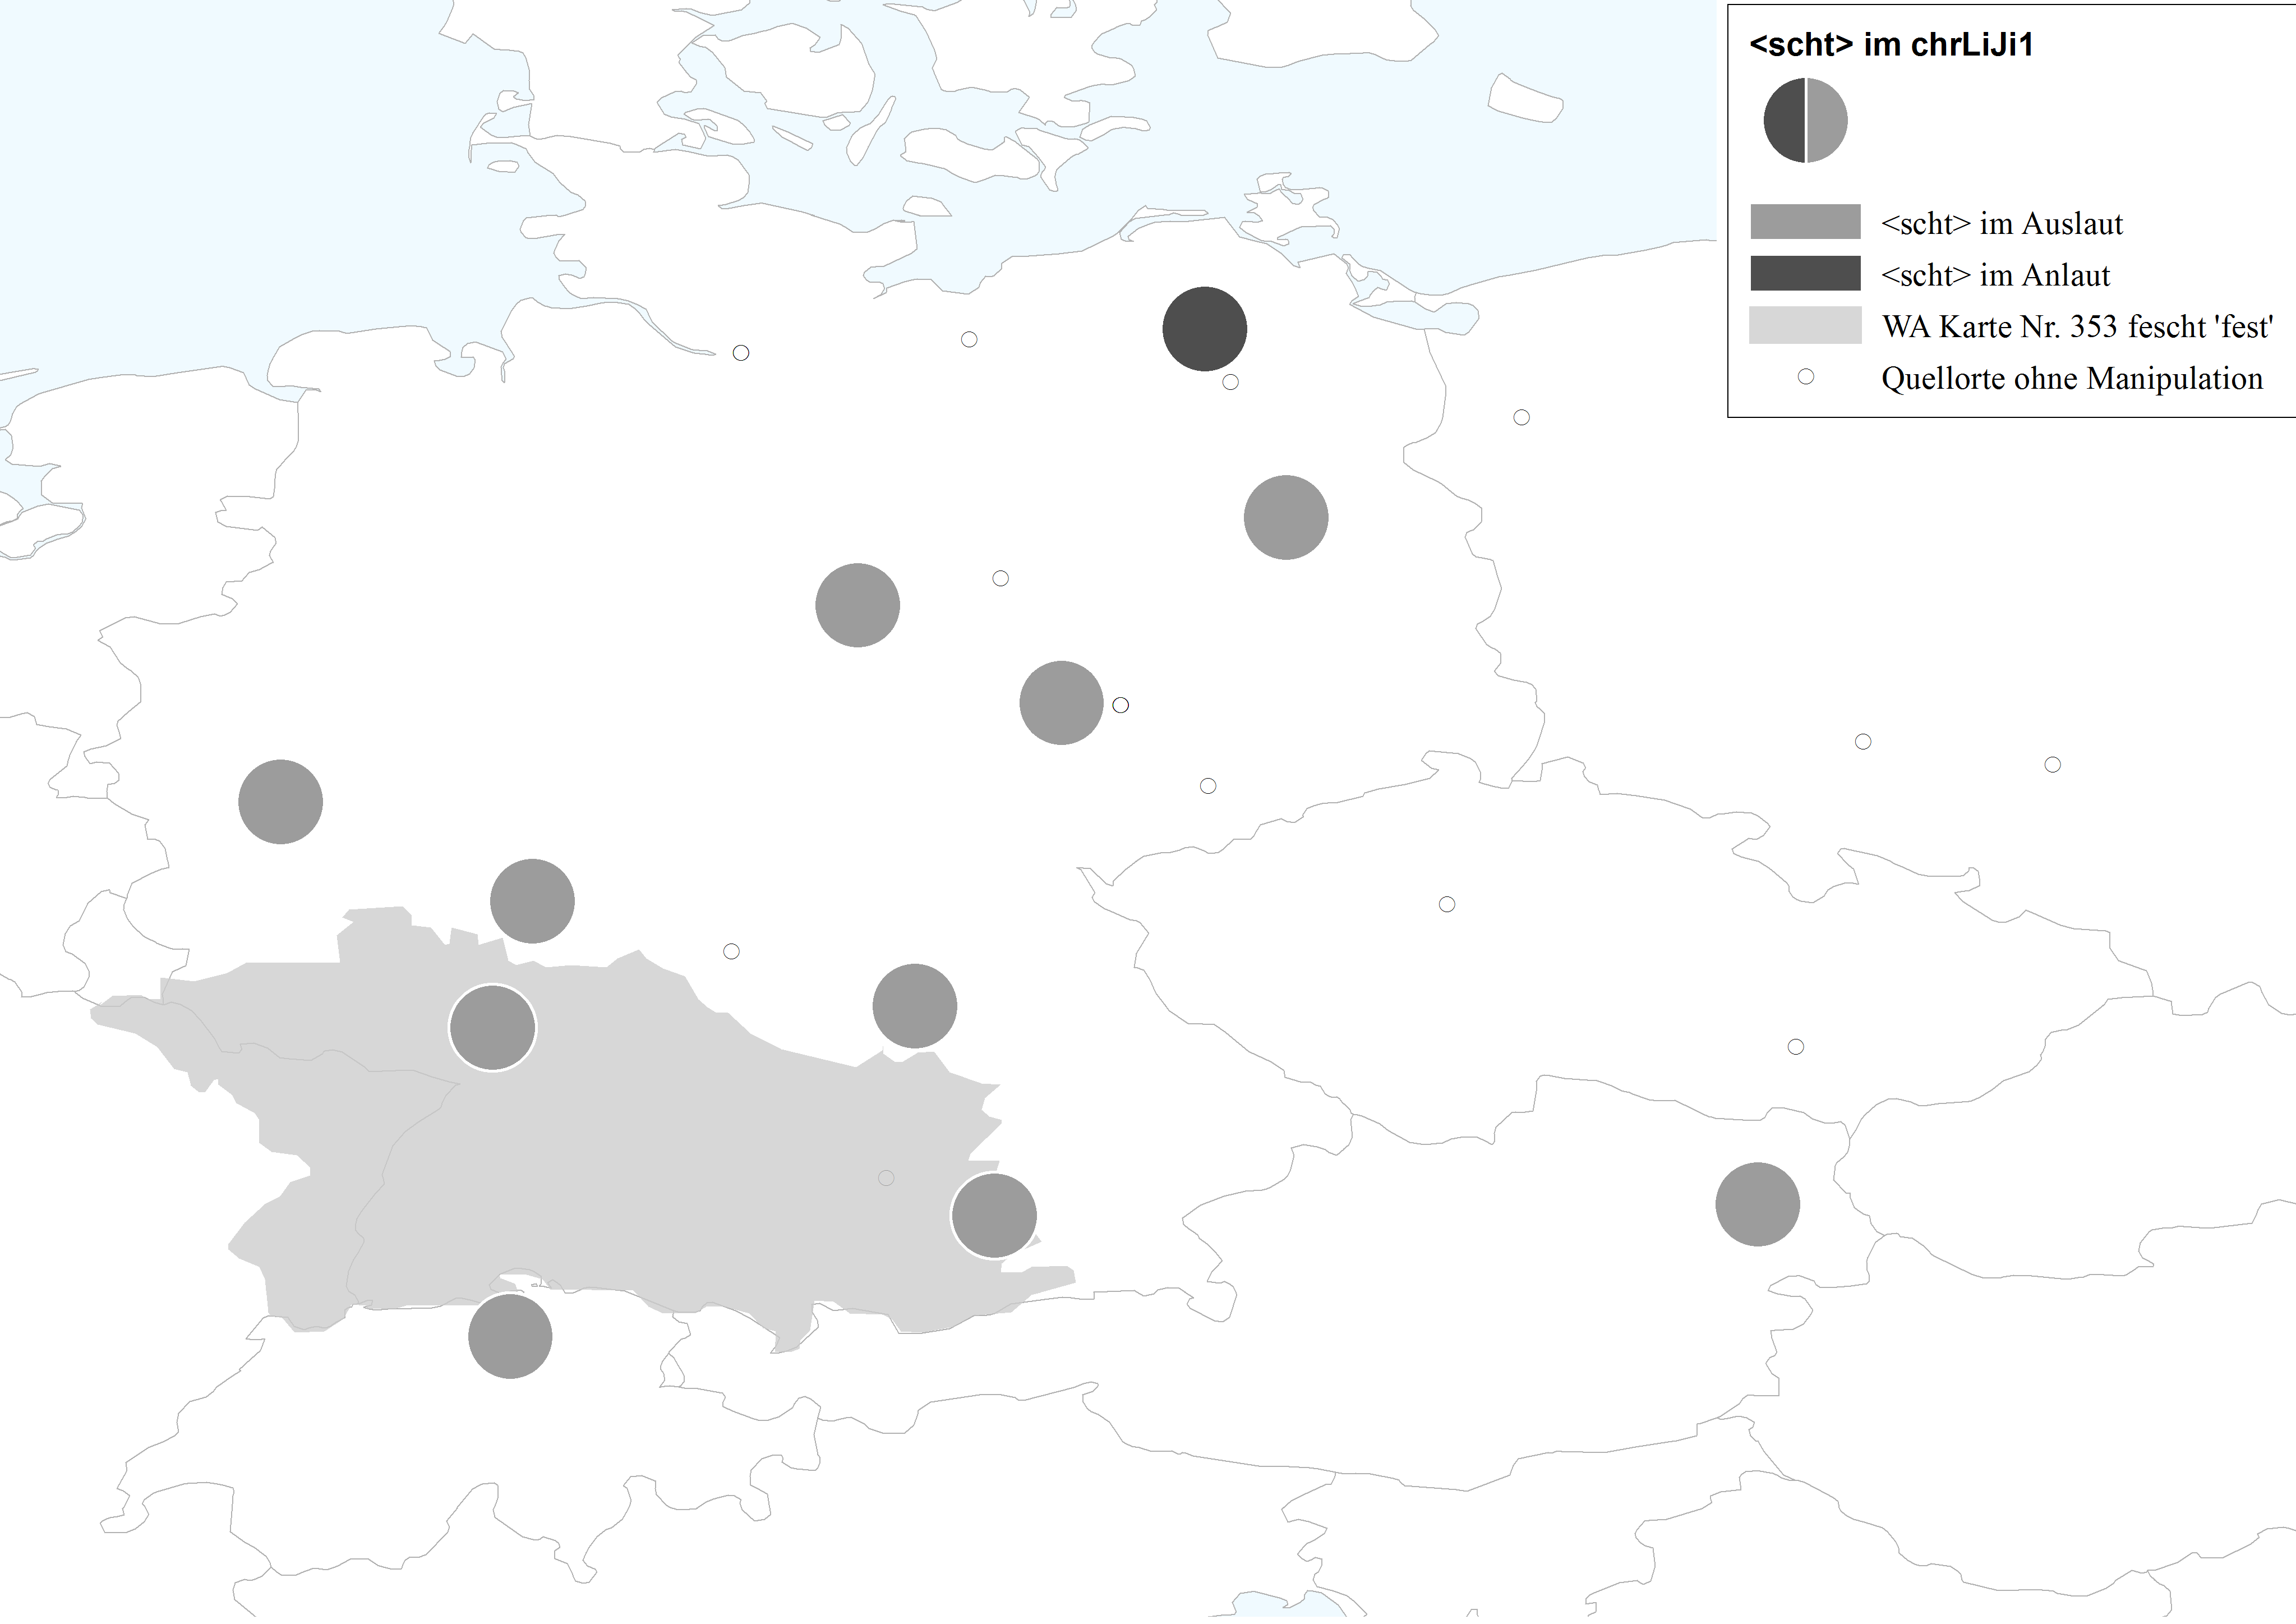
\includegraphics[scale=0.5]{figures/scht_karte.png}
		\caption{\label{kartescht} Die Graphie <scht> im \hai{chrLiJi1} mit \hai{WA} Karten Nr. 353}
		\end{figure}
\FloatBarrier


Die Belege aus dem Südwesten müssen aber nicht zwangsläufig Interferenzen zwischen \hai{LiJi} und den deutschen Dialekten sein, sondern können auch die tatsächliche Situation im örtlichen Westjiddischen erfassen. Zumindest zeigen die letzten Tonaufnahmen von Sprechern des \hai{SWJ} aus dem alemannischen Sprachgebiet der späten 50er und 60er Jahre eben dieses Phänomen, wie etwa in Bsp. \ref{bspschtalem1}–\ref{bspschtalem2b}.\\

 \eenumsentence{
 
 \item \textit{faʃtə} \sem{Fasten} (Endinger \hai{SWJ}; \cite[74]{Fleischer2005})
 \label{bspschtalem1}

 \item \textit{luʃtig} \sem{lustig} (Endinger \hai{SWJ}; \cite[74]{Fleischer2005})
 \label{bspschtalem1b}
 
 \item \textit{iʃ} \sem{ist} (Grussenheim (Oberelsass); \cite[43]{GuggenheimGruenberg1966})
 \label{bspschtalem2}
 
 \item \textit{maiʃti} \sem{meisten} (Grussenheim (Oberelsass); \cite[43]{GuggenheimGruenberg1966})
 \label{bspschtalem2b} 
 
 
 }
 

Man könnte nun annehmen, dass diese Formen im \hai{SWJ} auf den starken \isi{Sprachkontakt} zum Alemannischen zurückgeführt werden können, welcher besonders stark v.\,a. auf morphosyntaktischer Ebene auf das Jiddische gewirkt hat (vgl. \cite{Schaefer2014}). Doch Belege aus anderen Regionen zeigen, dass die \isi{Palatalisierung} nicht zwangsläufig auf den alemannischen \isi{Sprachkontakt} zurückzuführen ist, sondern auch ein autochthon jiddisches Phänomen ist, s. Bsp. in \ref{bspwjscht}. \textcite[98f]{GuggenheimGruenberg1958}, \textcite[20]{Beem1970} und Beraneks \hai{WjSA} (Karte Nr. 39) gehen davon aus, dass die \isi{Palatalisierung} im In- und \isi{Auslaut} im gesamten \hai{WJ}, mit Ausnahme des östl. \hai{NWJ}, vollzogen wurde; jedoch liegen kaum Analysen zur Systematik dieses Phänomens vor. Im \hai{ZWJ} der \qu{Hochzeit zu Grobsdorf} etwa findet sich \RL{<שט>} im In- und \isi{Auslaut}, Bsp. \ref{bspgrob20}–\ref{bspgrob22}; in deutschsprachigen Sequenzen bzw. auf dem Titelblatt findet sich hingegen \RL{<סט>} gesetzt, Bsp. \ref{bspgrob23}. \RL{<שט>} steht allerdings nie nach Nasal, Bsp. \ref{bspgrob24}–\ref{bspgrob25}. Darin verhält sich der Text äußerst homogen. Auch das \hai{NWJ} Aurichs zeigt, in unmissverständlicher lateinischer \isi{Orthographie}, dieses Phänomen, Bsp. \ref{bspaurich1}–\ref{bspaurich2}. Anders als im \hai{OJ}, s. Bsp. \ref{bspschtverb1}–\ref{bspschtverb2}, findet sich die Koronialisierung in der hessischen Quelle auch bei Verben, z.\,B. \ref{bspgrob25}.  Eine  Systematik wie im \hai{OJ} oder im \hai{WJ} der \qu{Hochzeit zu Grobsdorf} gegeben, lässt sich im \hai{LiJi} jedoch nicht erkennen. Nirgends im \hai{WJ} ist aber die \isi{Palatalisierung} von /st/ im In- und \isi{Auslaut} dermaßen konsequent durchgeführt, wie im westl. \hai{SWJ}; der alemannische Einfluss mag hier also gewirkt haben.\\

   \eenumsentence{
 \item  \RL{לושטיג}  \textit{lusshtig} \sem{lustig} (\qu{Die Hochzeit zu Grobsdorf} 1822:\,10) 
\label{bspgrob20} 

 \item  \RL{ערשטת} \textit{erscht} \sem{erst} (\qu{Die Hochzeit zu Grobsdorf} 1822:\,8, 12, 14)
\label{bspgrob21} 

 \item  \RL{ווא\makebox(-1.5,-7.5)[r]{\libertineGlyph{uni207B}}רשטע} \textit{varshte} \sem{wirst du} (\qu{Die Hochzeit zu Grobsdorf} 1822:\,27)
\label{bspgrob22} 

\item  \RL{לוסטיג} (in dt. Text) \textit{lustig} \sem{lustig} (\qu{Die Hochzeit zu Grobsdorf} 1822:\,Titel,  32) \label{bspgrob23} 
 
 \item \RL{זונסט} \textit{zunst} \sem{sonst} (\qu{Die Hochzeit zu Grobsdorf} 1822:\,12, 13, 14, 27)
\label{bspgrob24} 

 \item  \RL{קומסט} \textit{kumst} \sem{kommst} (\qu{Die Hochzeit zu Grobsdorf} 1822:\, u.\,a. 8)
\label{bspgrob25} 

\item \textit{geschtern} \sem{gestern} \parencite[125]{Reershemius2007}
\label {bspaurich1}
 
\item \textit{Erscht} \sem{erst} \parencite[125]{Reershemius2007}
\label {bspaurich2}

\item \textit{nischt} \sem {nicht} (Heymann 1909:\,5)
 
 }\label{bspwjscht}

Damit ist schwer zu entscheiden, ob in die südwestlichen Quellen des  \hai{chrLiJi1} Formen deutscher Dialekte in die \isi{Imitation} einflossen, oder ob die tatsächlich westjiddische Form durch den Umstand, dass die \isi{Assimilation} von /st/ an diesen Orten allgegenwärtig war, leichter für die Imitatoren zugänglich war, als andernorts.

Im \hai{jüdLiJi1} tritt die Schreibung <scht> nur sehr selten in Erscheinung. In fünf Texten findet sie sich im Aus- und Inlaut.\footnote{Die entsprechenden Quellen sind \hai{GuS5}, \hai{GuS23}, \hai{PAlsleben}, \hai{PBerlin1} u. \hai{PBerlin2}.} Insbesondere ist hier das Lexem \sem{erste} betroffen, welches in drei Quellen\footnote{\hai{GuS5}, \hai{PAlsleben} u. \hai{PBerlin1}.} die einzige Manipulation zu <scht> aufweist. Eine Quelle, \hai{PBerlin2}, legt besonderen Wert darauf, die hochdeutsche bzw. jiddische Aussprache im \isi{Anlaut} zu verschriftlichen; sonst spielt diese keine Rolle im \hai{jüdLiJi1}. Es irritiert, dass \hai{jüdLiJi1} hier scheinbar weniger authentisch ist, als das \hai{chrLiJi1}.


Selbst, wenn dieses Phänomen nicht zu den frequentesten Manipulationsstrategien des \hai{LiJi} zählt, so zeigt es doch um ein weiteres Mal, dass \hai{chrLiJi1} auf phonologischer Ebene näher an der tatsächlichen Sprachrealität des \hai{WJ} ist, als \hai{jüdLiJi1}. Dieses Bild kann natürlich der Unausgewogenheit der drei Teilkorpora geschuldet sein. Dass uns aber kaum Belege für die \isi{Palatalisierung} von /st/ im In- und \isi{Auslaut} aus den kleineren Korpora vorliegen, darf als Indiz dafür gelten, dass deren Konzepte von literarischem Jiddisch andere Prioritäten setzen als das \hai{chrLiJi1}. 


\subsection{\isi{Koronalisierung} <ch> > <sch>}\label{ch}
%  %\noindent
Elf Texte des \hai{chrLiJi1} verwenden die \isi{Koronalisierung} von /ҫ/ <ch> zu /ʃ/ <sch>  im Lexem \sem{nicht} < mhd. \textit{niht} \parencite[Bd. 2, Sp. 83]{Lexer1992}. Hier fällt besonders die lexematische Gebundenheit der \isi{Imitation} auf. Die \isi{Koronalisierung} wurde scheinbar nicht als Regel erkannt, sondern nur als Alternativform eines Lexems.  

Die diachrone Verteilung der Quellen mit einer Verschriftlichung der \isi{Koronalisierung} von /ҫ/ zu /ʃ/ zeigt, dass diese erst ab dem 19. Jahrhundert ins \hai{chrLiJi1} Eingang findet (s. Histogramm in Abb. \ref{histoch}).\\


    %%%V12/13Diagramm%\begin{flushleft}	
\begin{figure}[h!]
	\begin{tikzpicture}
		\begin{axis}[only marks, width=0.82\textwidth,height=0.2\textheight,
		legend style={at={(1,1)},xshift=+0.2cm, yshift=-0.7cm,anchor=north west,nodes=left},
			%title={Funktionstypen des sp\"aten Westjiddisch},
			xtick={1700, 1725, 1750, 1775, 1800, 1825, 1850, 1875, 1900, 1925, 1950, 1975}, ytick=\empty,
			x tick label style={/pgf/number format/1000 sep=}, 
			y tick label style={/pgf/number format/1000 sep=},
			%extra y ticks={456.1, 1022.4},
			%extra y tick labels={{456,1},{1022,4}},
			extra y tick style={grid=major,
				tick label style={, ,}},
				ymin=0.7,
				ymax=2.9,
			ylabel={Phänomenbelege},
			enlarge x limits=0.03]	
	
			
\addplot [mark=*, black] table [x=jahr, y=ch] {figures/ch.txt}; %2

\addplot [mark=o, black] table [x=jahr, y=no] {figures/ch_no.txt}; %1.5


 

			% Andere Formen a={mark=square*,blue},% b={mark=triangle*,red},% c={mark=o,draw=black}}
						\legend{\textit{nischt}, unmanipuliert} %macht Legende
		\end{axis}
	\end{tikzpicture}
	\caption{\isi{Koronalisierung} von \sem{nicht} im \hai{chrLiJi1}}
	\label{histoch}	
\end{figure}
\FloatBarrier
  
Ausnahmsweise wurde für die geographische Darstellung eine Karte aus dem umstrittenen \hai{WjSA} von Beranek angeführt, da hier eine interessante Vergleichskarte zum Lexem \sem{nicht} vorliegt (s. Abb. \ref{kartenischt}). Nach Beranek findet sich \textit{nischt} vom \hai{NÜJ} bis ins östl. \hai{NWJ} hinein, für das restliche Gebiet des \hai{WJ} gibt Beranek \textit{niks} als die vorherrschende Form an. Im \hai{OJ} ist sowohl \RL{נישט} \textit{nisht} wie auch \hai{ניט} \textit{nit} verbreitet. Nach \textcite[375]{Bin-Nun1973} gestaltet sich die areale Verbreitung so, dass die nicht-koronalisierten Formen \textit{niks} im \hai{SÜJ} und \textit{nit} im \hai{NOJ} auftreten, \textit{nischt} hingegen im restlichen Teil des \hai{WJ} sowie in \hai{ZOJ} und \hai{SOJ}. 

Im Deutschen hat sich eine vergleichbare \isi{Koronalisierung} erst im 19. Jahrhundert, ausgehend von Stadtmundarten im Westen des Sprachgebiets herausgebildet \parencite[97–101]{Herrgen1986}. Im Rhein- und Moselfränkischen und Ripuarischen ist /ҫ/ mit  [ʒ] konsequent zusammengefallen (\cite[275]{Schirmunski1962}; \cite{Herrgen1986}). Eine solche Regelmäßigkeit der \isi{Koronalisierung}, wie auch eine Entwicklung zu  [ʒ] liegt im Ost- wie Westjiddischen nicht vor. Das Lexem \sem{nicht} stellt eine Ausnahme dar. Neben den fränkischen Dialekten ist die Form \textit{nischt} auch für das Osthessische und Obersächsische beschrieben (\hai{DWB} \citeyear[Bd. 13, Sp. 729]{DeutschesWB}). Im Wenkeratlas zeigt sich die \isi{Koronalisierung} weit im Ostmitteldeutschen und den Mundarten der nordostdeutschen Siedlungsmundarten (vgl. \hai{WA} Karte Nr. 537 \sem{nichts}).\\

 \begin{figure}[h!]
		\centering
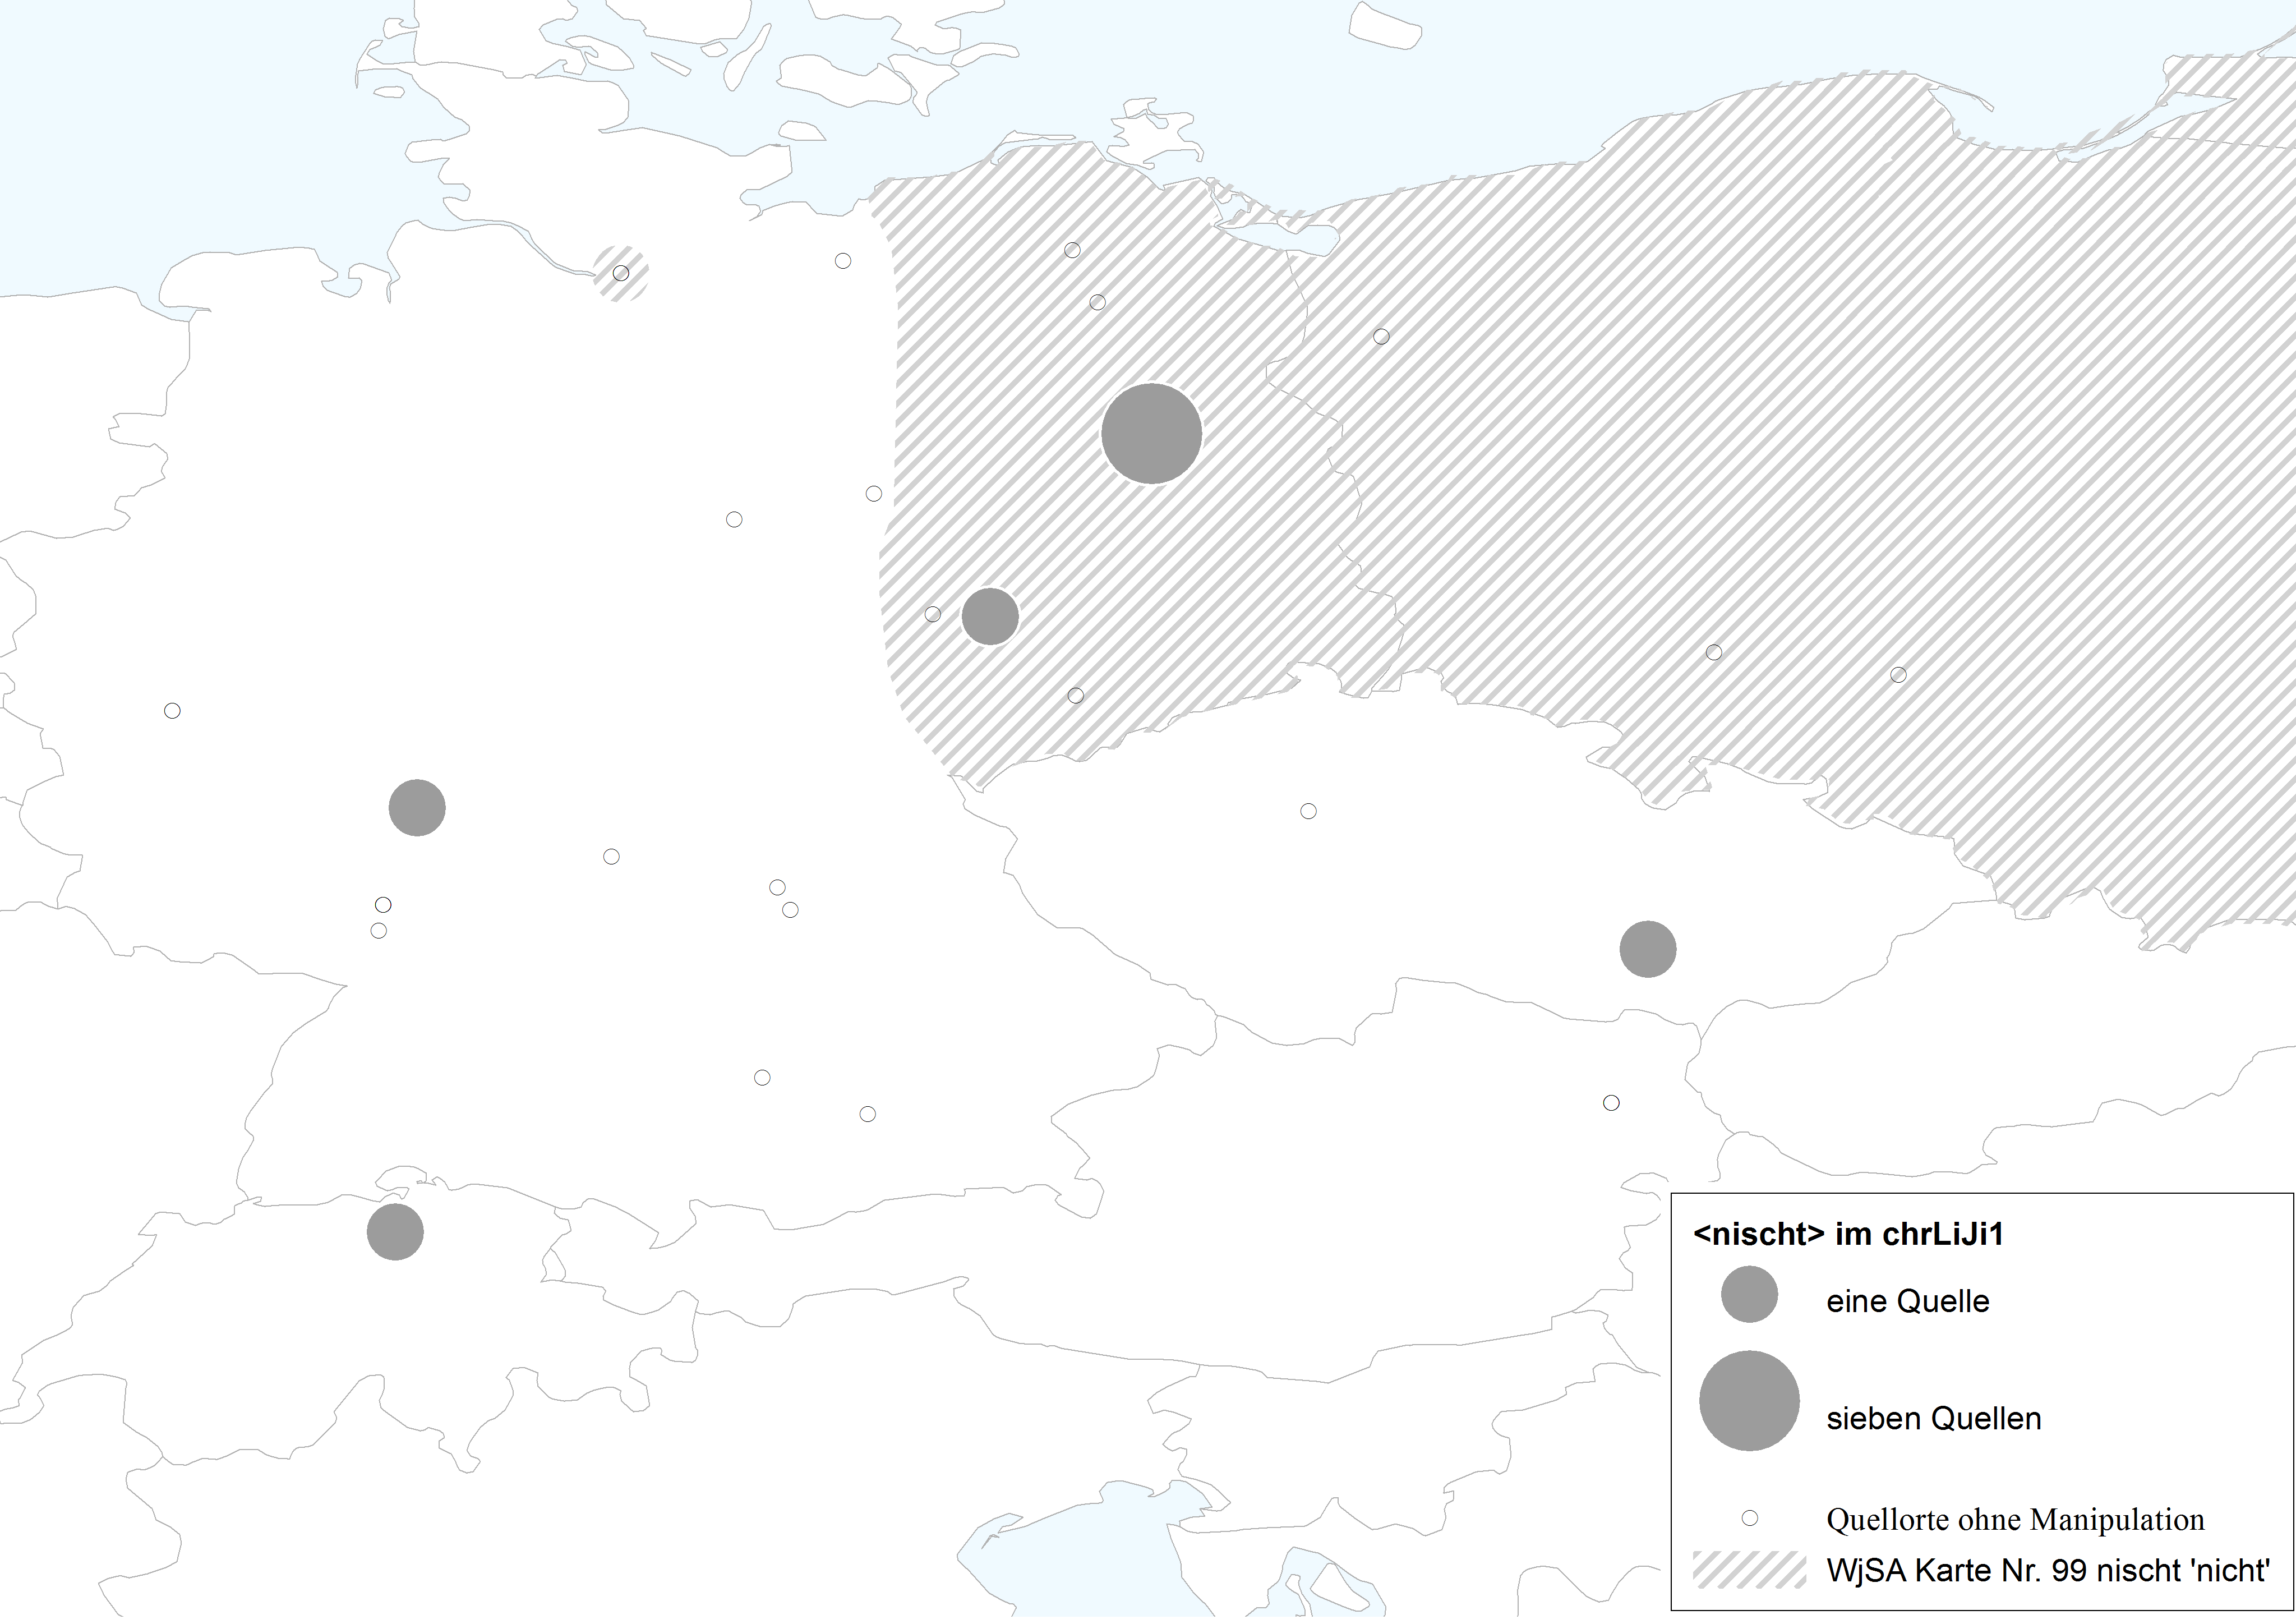
\includegraphics[scale=0.5]{figures/nischt_karte.png}
		\caption{\label{kartenischt} \textit{nischt} im \hai{chrLiJi1} mit \hai{WjSA} Karte Nr. 99}
		\end{figure}
\FloatBarrier
		
 Im kartographischen Vergleich zum \hai{chrLiJi1} fällt auf, dass insbesondere Quellen aus Berlin und Leipzig die \isi{Koronalisierung} von <ch> im Lexem \sem{nichts} vornehmen. Die Zürcher  Quelle \hai{AK} (Zürich, 1948), die ebenfalls \textit{nischts} (\isi{Negationspartikel} als auch neg. Indefinitum) setzt, darf als vom \hai{OJ} beeinflusst angesehen werden. Die Frankfurter Quelle \hai{OF} (Frankfurt, 1711), die in den bisherigen Analysen immer sehr nah am \hai{WJ} war, verhält sich mit der \isi{Koronalisierung} besonders untypisch. Hier kann u.\,U. das Frankfurter Rheinfränkisch hineingewirkt haben.

Als ein Beispiel, dass der \hai{WjSA}, welcher mit Vorsicht zu genießen ist (vgl. \cite{GuggenheimGruenberg1966b}), in diesem Fall ein glaubwürdiges Bild vermittelt, seien hier zwei authentische westjiddische Quellen zu nennen: Die Autobiographie des Berliners Aron Hirsch Heymann aus den 1880er Jahren (vgl. \cite{Schaefer2013}) und die bereits bekannte hessische Quelle \qu{Die Hochzeit zu Grobsdorf}. Bei Heymann findet man die für das östl. \hai{NWJ} kartierte Form, Bsp. \ref{bspchhey}, wohingegen die Quelle aus dem westl. \hai{ZWJ}, die von Beranek für diesen Teil des \hai{WJ} übliche Form zeigt, Bsp. \ref{bspchgrob}.\\

 \eenumsentence{

\item \textit{nischt(s)} \sem {nicht(s)} (Heymann 1909:\, u.\,a. 5, 6, 7, 10, 13) \label{bspchhey}

\item \RL{ניקס} \textit{niks} \sem{nichts} (\qu{Die Hochzeit zu Grobsdorf} 1822:\, u.\,a. 4, 6, 10, 11, 12) \label{bspchgrob}


}

Sechs der sieben Berliner Quellen des \hai{jüdLiJi1} verwenden, entsprechend der arealen Struktur, \textit{nischt}.\footnote{Die Quellen mit der \isi{Koronalisierung} \textit{nischt} sind: \hai{GuS1}, \hai{GuS5}, \hai{GuS10}, \hai{GuS15}, \hai{GuS23} u. \hai{PBerlin2}.} Die übrigen Texte des \hai{jüdLiJi} manipulieren dieses Lexem nicht.\\

 
Insgesamt fällt auf, dass die \isi{Koronalisierung} nicht als Regel umgesetzt wird, sondern nur an einem Lexem, wo sie der Form des östl. \hai{WJ} bzw. des \hai{OJ} entspricht. Dieses Phänomen zeigt eine besonders eindeutige areale Verbreitung im \hai{LiJi1}, die den bisher gewonnenen Daten zum \hai{WJ} entspricht.\\
%\clearpage



\section{\isi{Deaffrizierung} von <z>}\label{sz}
%\noindent
Zehn Quellen des \hai{chrLiJi1} verwenden eine auffällige Graphie der stimmlosen alveolaren Affrikate /ts/ <z> im \isi{Anlaut}, indem sie stattdessen <s> oder <ß> setzen. Besonders betroffen ist das Lexem \sem{zu}, welches als \textit{su} (\hai{AH} Chemnitz, 1789:\,2, 3; \hai{BS} Mannheim, 1798:\,4; \hai{BW} Leipzig, 1826 Leipzig, 1826:\,99; \hai{PF} Augsburg, 1816:\,12, 13; \hai{VD} Frankfurt, 1916:\,13, 15, 19) oder als \textit{ßu} (\hai{AJ} Berlin, 1825:\,2, 4, 6; \hai{DP} Pyrzyce, 1874:\,15, 19, 29; \hai{SV} München, 1890:\, IV, 1, 3, 5, 6, 7; \hai{UT} Stavenhagen, 1862:\,Kap. 45) auftaucht. Hinter dieser \isi{Orthographie} könnte sich eine \isi{Deaffrizierung} zu einem \isi{Frikativ} verbergen. <ß> kann etwa auf stimmloses [s] verweisen; <s> kann sowohl für stimmloses [s] wie auch stimmhaftes [z] stehen. Diese \isi{Deaffrizierung} ist prinzipiell eine im Hochdeutschen mögliche Entwicklung. Analog zu Prozessen im Ostmitteldeutschen, wo die aus der 2. \hai{LV} hervorgegangene Affrikate /pf/ zu /f/ lenisiert wurde, z.\,B. [pfʊnt] > md. [fʊnt], kann sich auch /ts/ > /s/, /z/ entwickelt haben (vgl. \cite[273, 282]{Schirmunski1962}; \cite[64f]{Koenig1978}; \hai{KDSA} Karten Nr. 21, 22). Im modernen \hai{OJ} fand dieselbe Weiterentwicklung von anlautendem germ. \textit{p} > mhd. \textit{pf} zu \textit{f} statt (im \isi{Auslaut} > \textit{p}) (\cite[189]{Kleine2008}; \cite[323–327]{Bin-Nun1973}). Diese wird auch graphematisch umgesetzt, z.\,B. \RL{פֿערדל} \textit{ferdl} \sem{Pferdchen}. Würde es sich bei der Entwicklung /ts/ > /s/, /z/ um eine analoge Ausdehnung, bzw. logische Weiterführung der 2. \hai{LV} handeln, so wäre diese für das Jiddische demnach nicht auszuschließen. Der Karte Nr. 57 des \hai{LCAAJ} zufolge, blieb die Affrikate /pf/ im \hai{WJ} allerdings weitgehend erhalten.  Für die jiddischen Varietäten ist allerdings eine \isi{Deaffrizierung} von anlautendem /ts/ nicht bekannt. Und nur im \hai{NWJ} und östl. \hai{ZWJ} findet sich dort die Weiterentwicklung zu /f/. Doch lässt die Setzung von <\RL{פֿ}> bzw. <\RL{פ}> im westl. \hai{ZWJ} der \qu{Hochzeit zu Grobsdorf} darauf schließen, dass hier der \isi{Frikativ} /f/, bzw. ggf. auch der Plosiv /p/, verwendet wurde; zumindest findet sich keine Affrikate verschriftlicht, s. Bsp. \ref{bspgrobsdorfpf1}--\ref{bspgrobsdorfpf2}. Im Gegensatz zur \isi{Deaffrizierung} von /ts/ > /s/, /z/ spielt die von /pf/ > /f/ für das \hai{LiJi} interessanterweise keine Rolle.\footnote{Lediglich in einer Quelle des \hai{jüdLiJi1} finden sich zwei Belege: \textit{Ferd} \sem{Pferde} (\hai{GuS4}:\,5), \textit{Fennig} \sem{Pfennig} (\hai{GuS4}:\,5).} \\%Im \hai{LiJi2} findet sich sogar einmal die unverschobene und dem Jiddischen nicht entsprechende Form in \textit{Dreiviertelpund} \sem{3/4 Pfund} (\hai{TFRdt}:\,98).}\label{punt} \\

\pagebreak

 \eenumsentence{

\item \RL{פעננינג} \textit{pennig}, \textit{fennig} \sem{Pfennige} (\qu{Die Hochzeit zu Grobsdorf} 1822:\,38)\label{bspgrobsdorfpf1}

\item \RL{פֿונט} \textit{funt}, \sem{Pfund} (\qu{Die Hochzeit zu Grobsdorf} 1822:\,42, 134)\label{bspgrobsdorfpf2}

}


Eine Setzung von /s/ an der Position von nhd. /ts/ wurde im An- und Inlaut besonders im Lothringischen und Moselfränkischen durchgeführt, ist aber auch im Niederdeutschen zu finden, wo es nach \textcite[282]{Schirmunski1962} v.\,a. in hochdeutschen Entlehnungen als Hyperkorrektur auftritt. Nach der \hai{KDSA} Karte Nr. 47 findet sich /ts/ > /s/ zumindest im Lexem \textit{zum} auch im Mittelbairischen und vereinzelt im burgenländischen Südmittelbairischen (vgl. Abb. \ref{karteszkdsa}). \textcite[282, 273]{Schirmunski1962} vertritt für die mittel- und niederdeutschen Dialekte die Hypothese, dass die Setzung von /s/ bzw. /f/ auf den Einfluss der Standardsprache (\qu{Ausgleichsform}) zurückzuführen ist, da die standarddeutschen Affrikate /ts/ und /pf/ in diesen Dialekten nicht gegeben sind. Sechs Quellen des \hai{chrLiJi1} verwenden <ß> für <z> (im \isi{Anlaut}); fünf Quellen setzen <s> für <z>. Die Quelle \hai{PF} (Augsburg, 1816) verwendet sowohl die Schreibung <ß> für <z> als auch die von  <s> für <z> und verhält sich somit als einziger Text in diesem Bereich nicht homogen.\\


\begin{figure}[h!]
	\begin{tikzpicture}
		\begin{axis}[only marks, width=0.82\textwidth,height=0.2\textheight,
		legend style={at={(1,1)},xshift=+0.2cm, yshift=-0.44cm,anchor=north west,nodes=left},
			%title={Funktionstypen des sp\"aten Westjiddisch},
			xtick={1700, 1725, 1750, 1775, 1800, 1825, 1850, 1875, 1900, 1925, 1950, 1975}, ytick=\empty,
			x tick label style={/pgf/number format/1000 sep=}, 
			y tick label style={/pgf/number format/1000 sep=},
			%extra y ticks={456.1, 1022.4},
			%extra y tick labels={{456,1},{1022,4}},
			extra y tick style={grid=major,
				tick label style={, ,}},
				ymin=0.7,
				ymax=2.9,
			ylabel={Phänomenbelege},
			enlarge x limits=0.03]	
	
			
\addplot [mark=*, black] table [x=jahr, y=sz_z] {figures/sz_z.txt}; %2.3
\addplot [mark=*, gray] table [x=jahr, y=s_z] {figures/s_z.txt}; %1.8
\addplot [mark=o, black] table [x=jahr, y=no] {figures/z_no.txt}; %1.3


 

			% Andere Formen a={mark=square*,blue},% b={mark=triangle*,red},% c={mark=o,draw=black}}
						\legend{<ß> für <z>, <s> für <z>,unmanipuliert} %macht Legende
		\end{axis}
	\end{tikzpicture}
	\caption{Graphien alveolarer Frikative im \hai{chrLiJi1}}
	\label{histosz}	
\end{figure}
\FloatBarrier



Wie die Karte in Abb. \ref{kartesz} zeigt, ergibt die Verteilung der Graphien <ß>, <s> für <z> sogar ein areales Raumbild. So wird <ß> vor allem in Quellen des östl. \hai{NWJ} gesetzt, während <s> für <z> im \hai{ZWJ} auftritt.\\


 \begin{figure}[h!]
		\centering
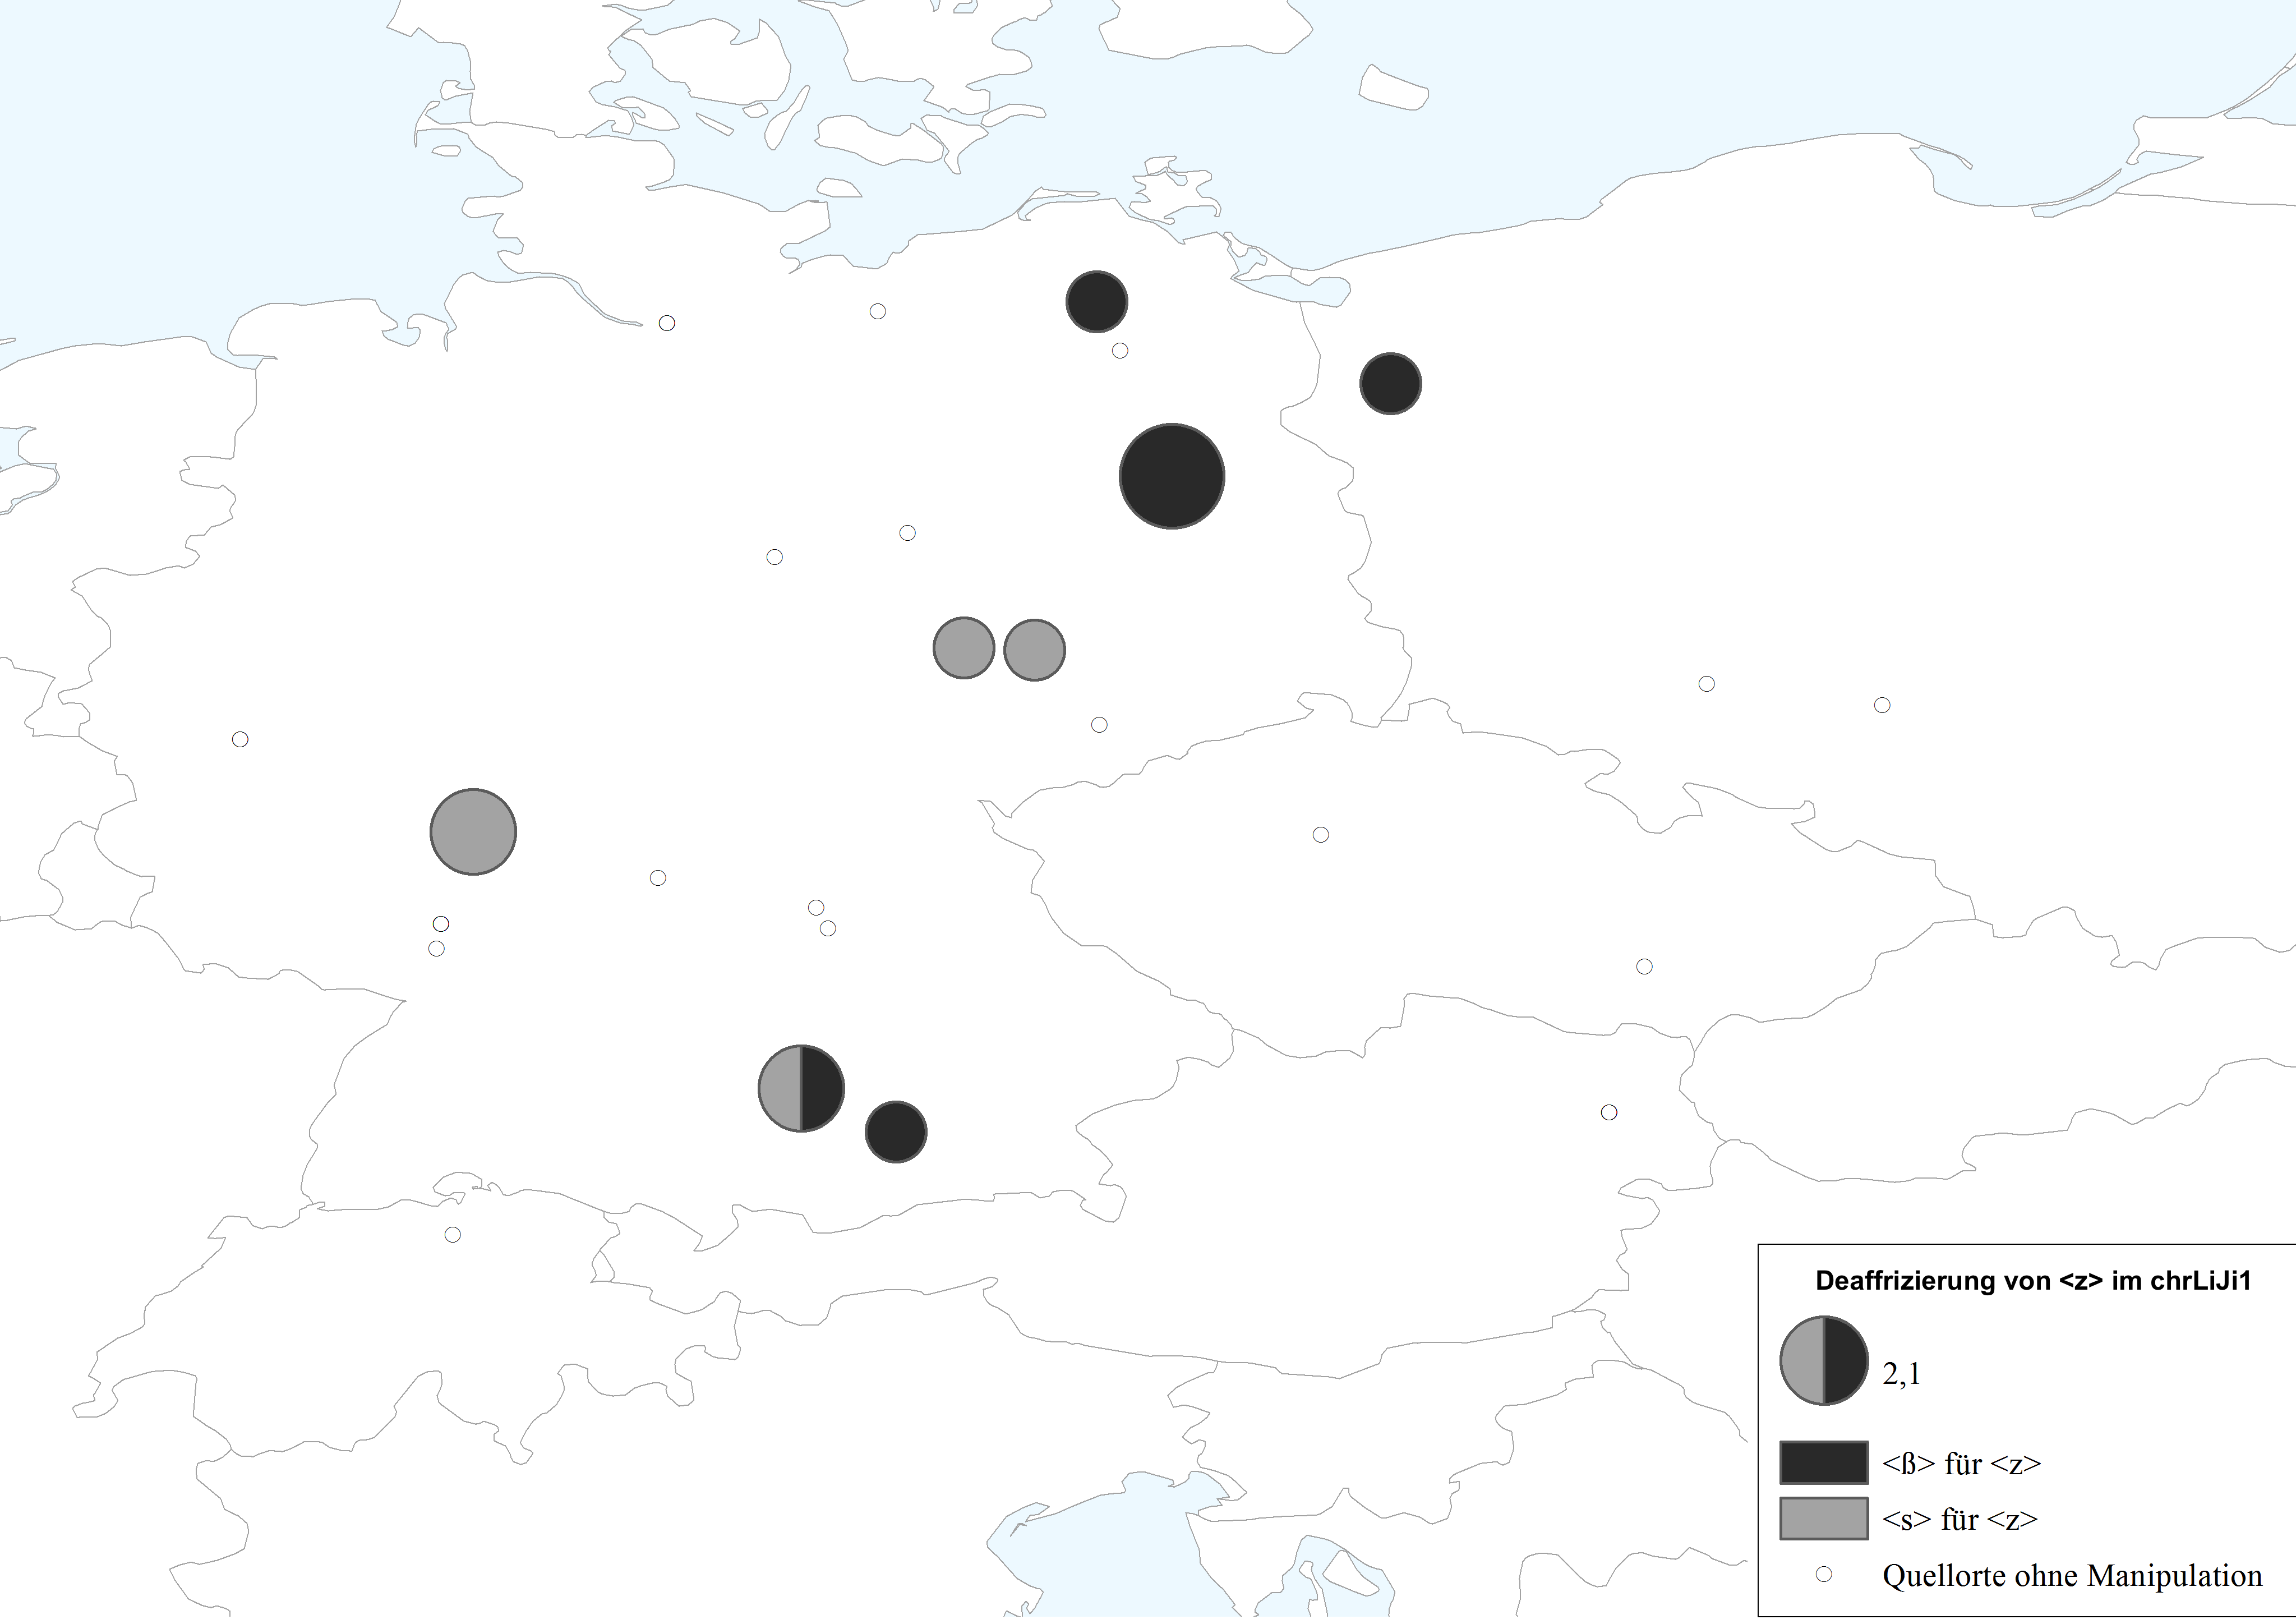
\includegraphics[scale=0.1]{figures/karte_sz.png}
		\caption{\label{kartesz} <ß>, <s> für <z> im \hai{chrLiJi1}}
		\end{figure}
\FloatBarrier


Dieses Raumbild erstaunt besonders vor dem Hintergrund, dass sich das östl. \hai{NWJ} in Bezug auf Affrikate und Frikative generell anders verhält, als das übrige \hai{WJ}. \textcite[1028]{Katz1983} stellt aufgrundlage von \textcite{Friedrich1784}, welcher im \isi{Anlaut} <s> für <z> setzt, fest, dass im \hai{NÜJ}\footnote{Obwohl Friedrich (\citeyear{Friedrich1784}) rein aufgrund der geographischen Verortung links der Oder eher zum \hai{NWJ} zu zählen ist.} die Affrikate /ts/ für anlautendes /s/ gesetzt werde. Der \hai{LCAAJ} (\citeyear[Karten 47, 48, 49]{Herzog1992}) zeigt zumindest, dass durch das westjiddische Sprachgebiet eine Isoglosse verläuft, die auf der Qualität des alveolaren Frikativs als stimmhaft [z] bzw. stimmlos [s] beruht (vgl. Abb \ref{karteszlcaaj}).\footnote{\textit{z} in den Karten des \hai{LCAAJ} entspricht der im englischen Sprachraum üblichen Notation für den stimmhaften \isi{Frikativ} [z].} 
Doch eine Markierung dieses Phänomens ($\pm$ stimmhaft) wird im \hai{LiJi} nicht verschriftlicht. Stattdessen wird mit der \isi{Deaffrizierung} von /ts/ <z> > /s/ <s>, <ß>, /z/ <s> eine gegensätzliche Entwicklung gezeigt. Das Areal der \isi{Deaffrizierung} im \hai{chrLiJi1} trifft jedoch auch relativ gut mit der Fortisierung im östl.\hai{NWJ} zusammen (s. Abb. \ref{karteszlcaaj}). Eine wenig plausible Erklärung für die Vermeidung des <z>-Graphems im \hai{chrLiJi1} könnte demnach sein, dass dort eigentlich die Fortisierung umgesetzt werden sollte, stattdessen aber eine \isi{Deaffrizierung} graphematisiert wurde. Diese Hypothese kann jedoch nicht erklären, wieso <s> für <z> im zentralwestjiddischen Gebiet des \hai{chrLiJi1} gesetzt wird. Plausibler scheint es, diese Graphien als Ausdruck einer \isi{Deaffrizierung} zu interpretieren, von deren Existenz im \hai{WJ} bislang jedoch nichts bekannt ist.\\

 \begin{figure}[h!]
		\centering
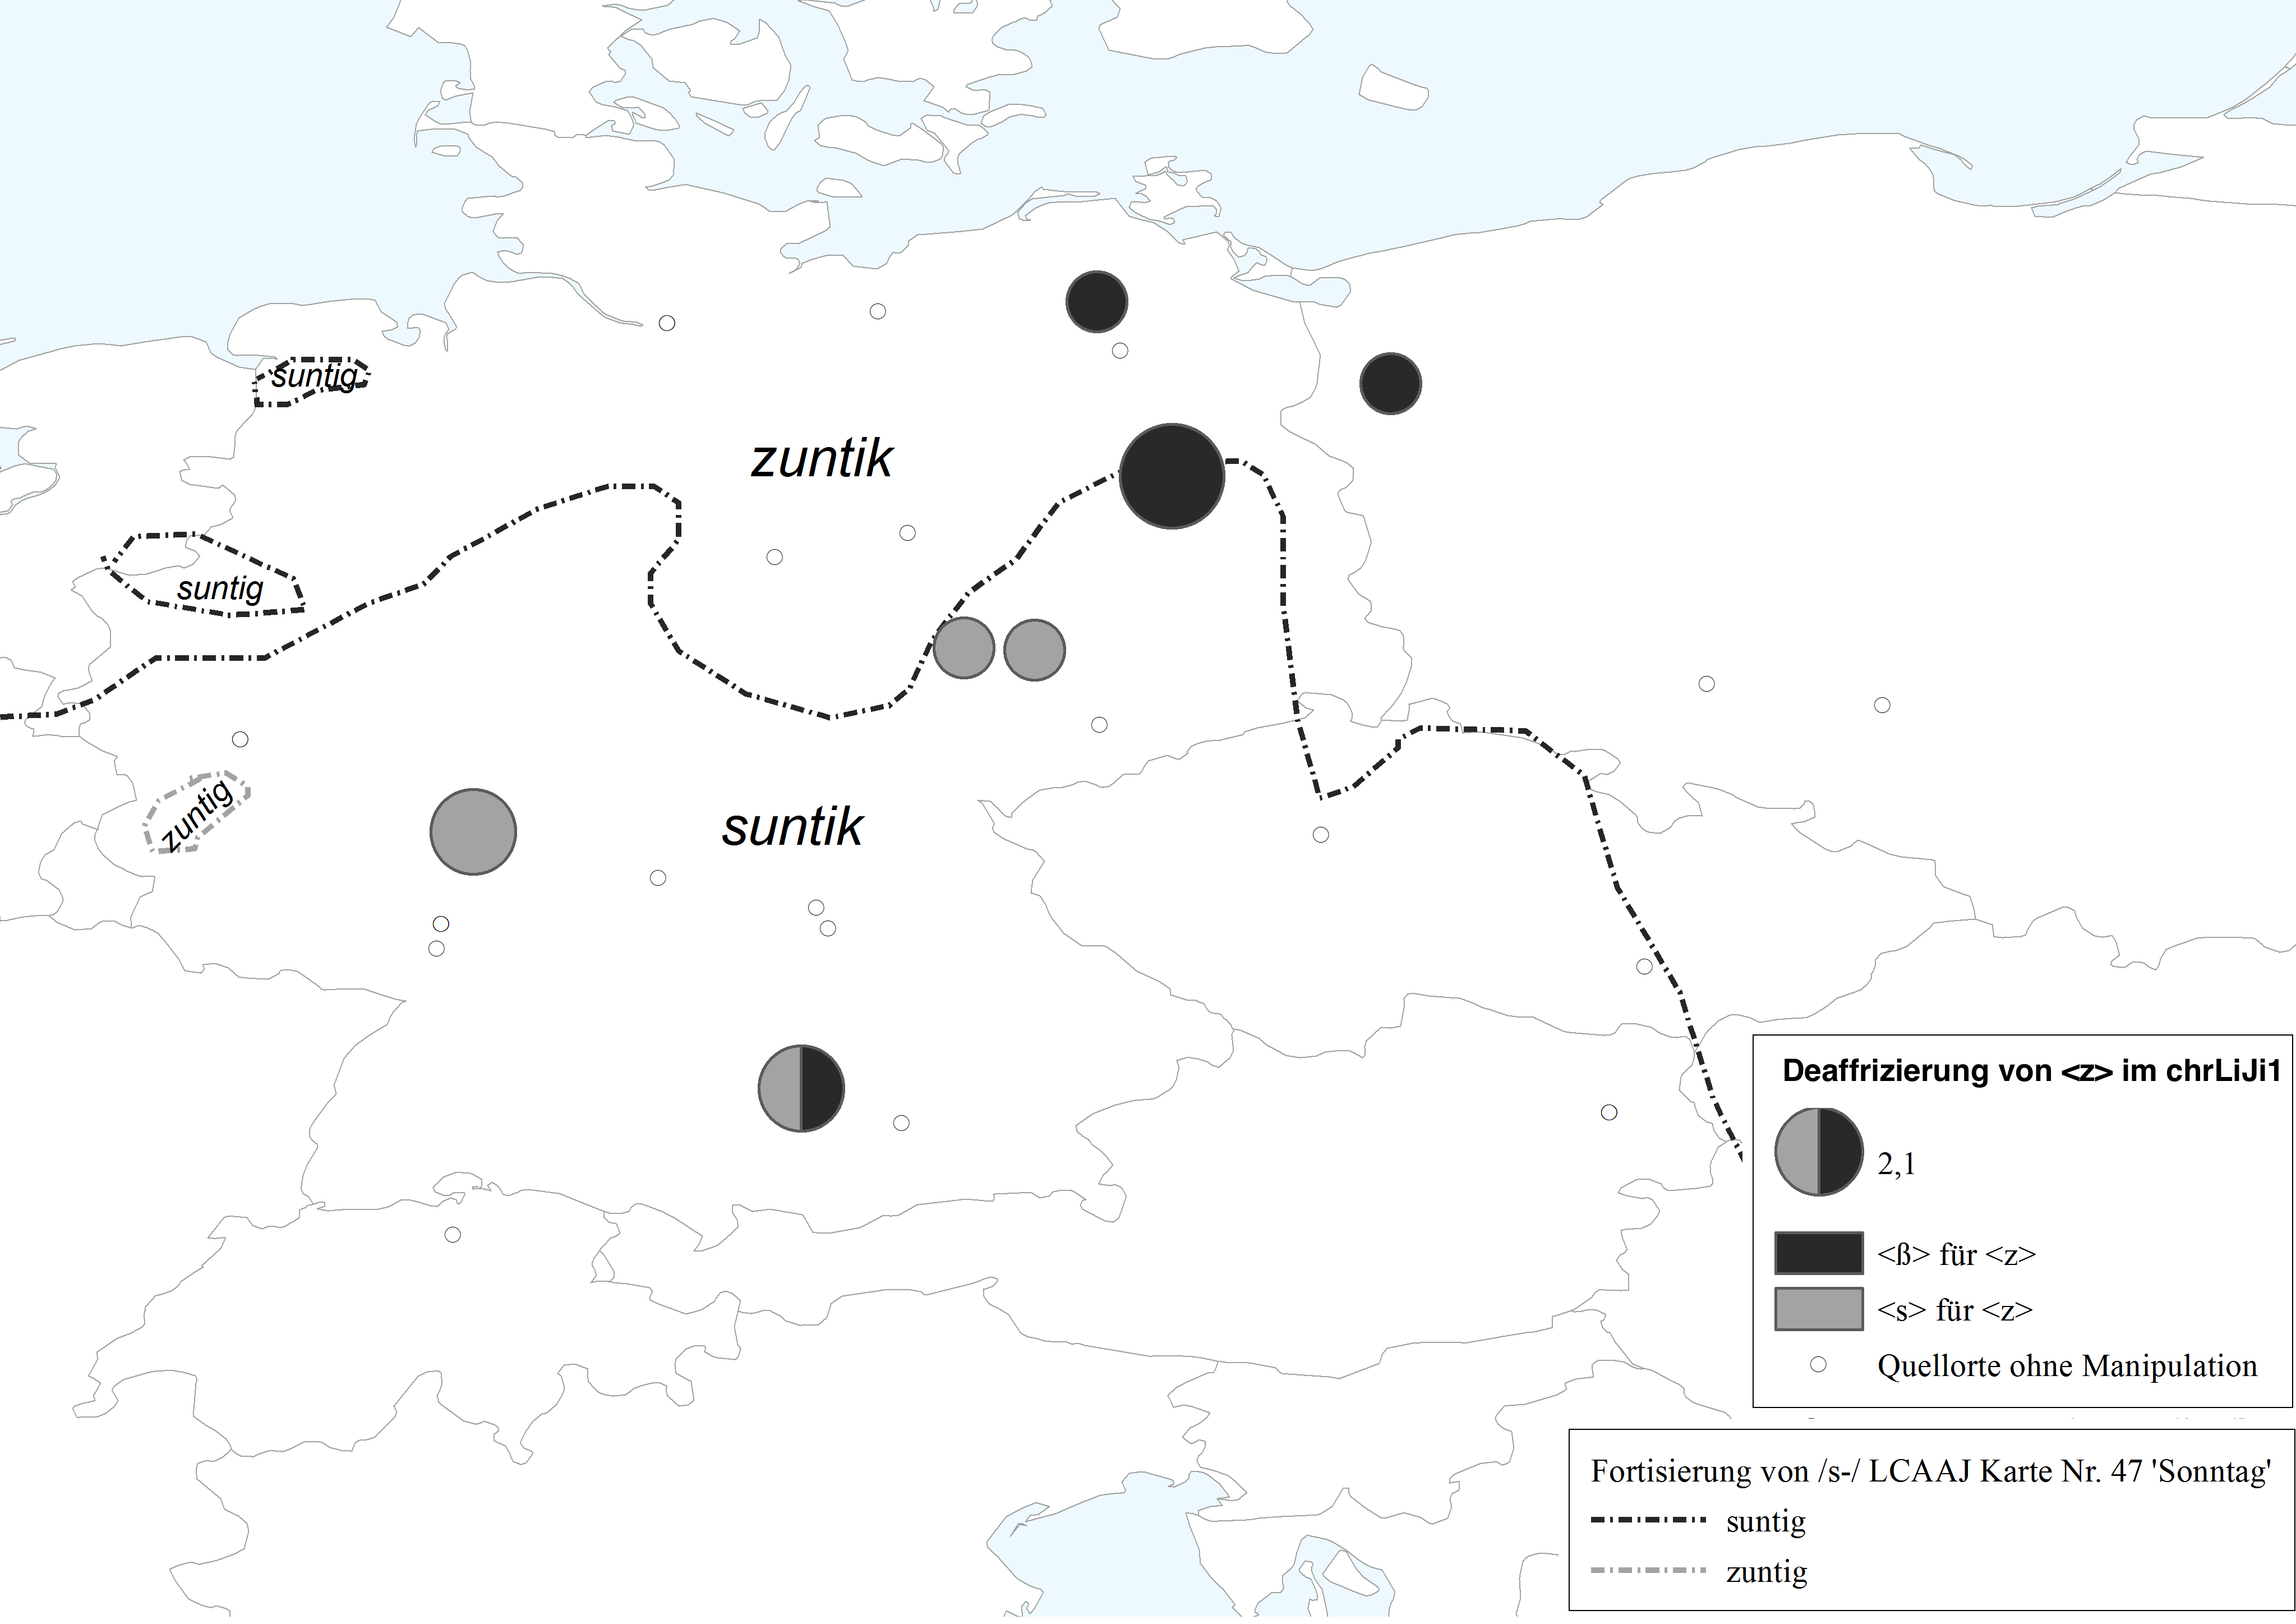
\includegraphics[scale=0.1]{figures/karte_sz_lcaaj.png}
		\caption{\label{karteszlcaaj} <ß>, <s> für <z> im \hai{chrLiJi1} mit \hai{LCAAJ} Karte Nr. 47}
		\end{figure}
\FloatBarrier



Die Belege von <s> für <z> in vier Quellen im Obersächsischen und Frankfurter Rheinfränkischen lassen sich auf Interferenzen aus den deutschen Dialekten ableiten. Wie die Karte in Abb. \ref{karteszkdsa} zeigt, ist genau in diesen Regionen die 2. \hai{LV} an anlautendem germ. \textit{t} weitergeführt worden zu /\textit{s}/. Es ist nicht auszuschließen, dass möglicherweise auch die örtlichen westjiddischen Varietäten an dieser Entwicklung teilgenommen haben. Allerdings fehlen bislang vergleichbare authentische Daten zum \hai{WJ} aus diesen Regionen, die dies bestätigen bzw. widerlegen. Auch die Belege für <ß> statt <z> im Nordosten können auf einer entsprechende Entwicklung von /ts/ > /s/ im Niederdeutschen beruhen (vgl. \cite[282]{Schirmunski1962}). Offen bleibt hierbei allerdings, warum das Graphem <ß> gewählt wurde und andernorts <s>. Gegebenenfalls wollten die Autoren mit der Setzung von <ß> die Stimmlosigkeit des Frikativs stärker hervorheben.\\


 \begin{figure}[h!]
		\centering
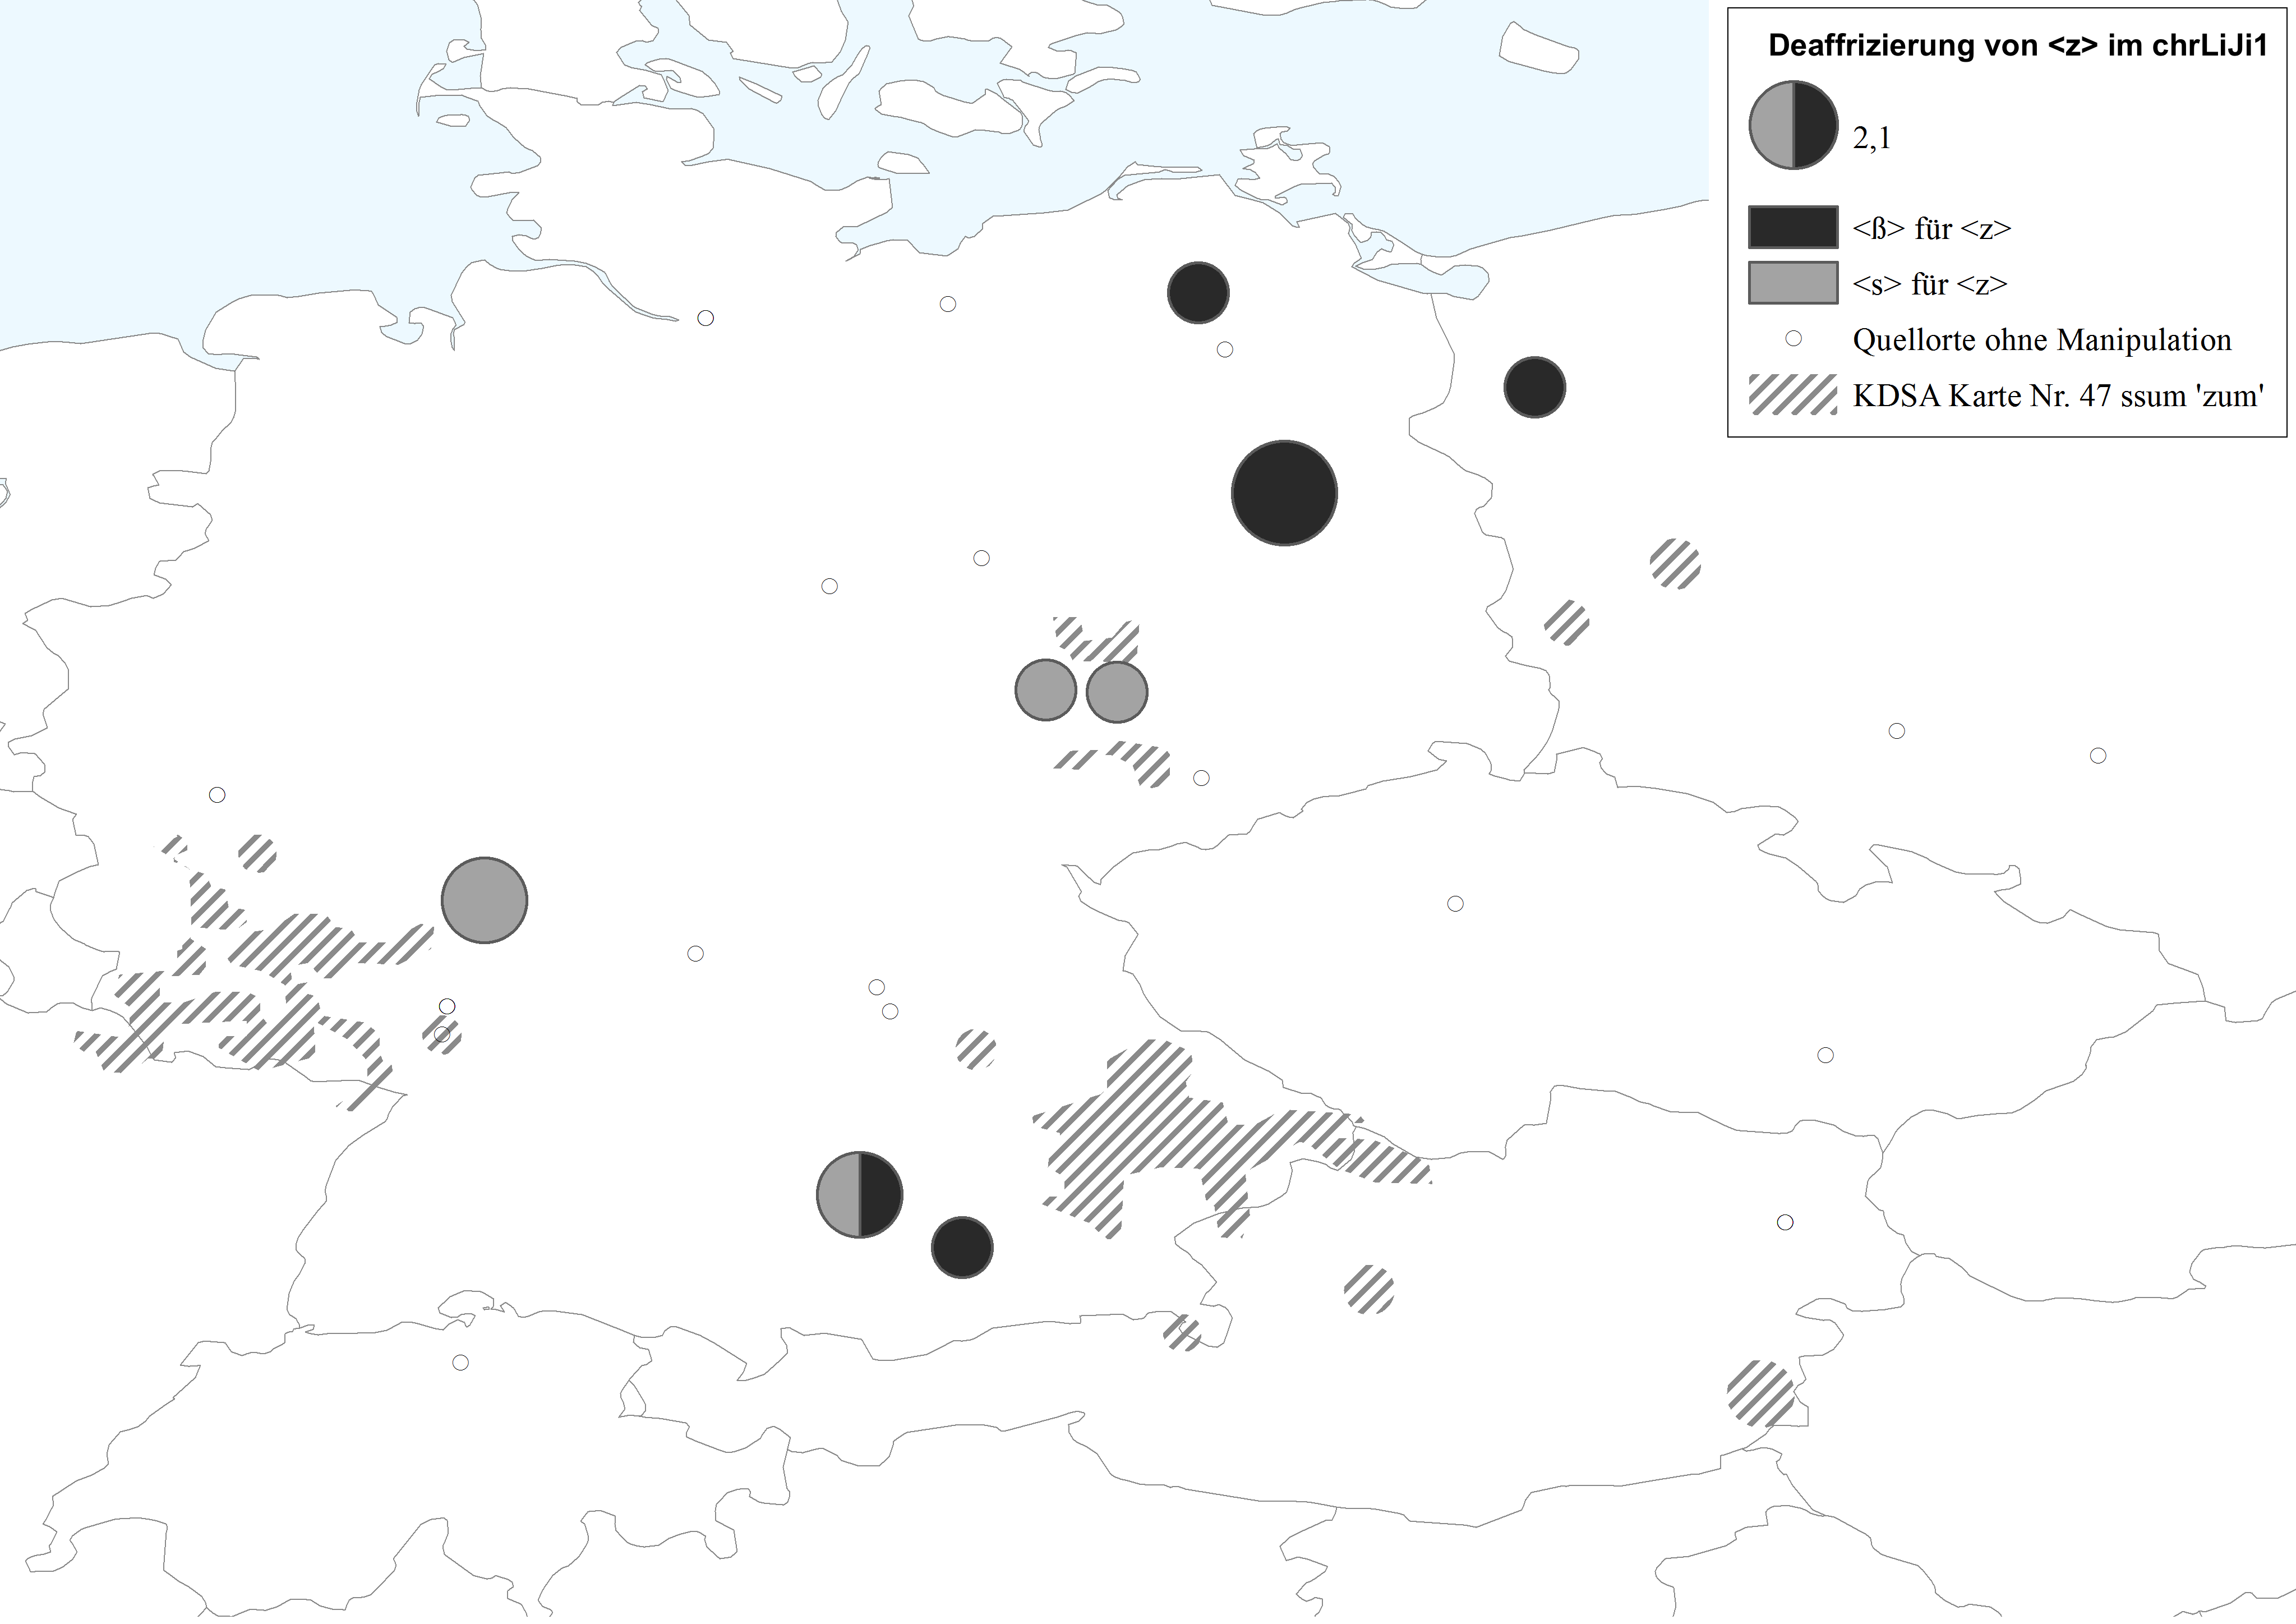
\includegraphics[scale=0.1]{figures/karte_sz_kdsa2.png}
		\caption{\label{karteszkdsa} <ß>, <s> für <z> im \hai{chrLiJi1} mit \hai{KDSA} Karte Nr. 47}
		\end{figure}
\FloatBarrier

%\clearpage 
<ß>-Graphien für <z> finden sich auch im \hai{jüdLiJi1} in drei Berliner Quellen und dem Pamphlet aus Alsleben.\footnote{Im Einzelnen sind diese Quellen: \hai{GuS10}, \hai{GuS23}, \hai{PAlsleben}, \hai{PBerlin2}.} Das verweist zumindest darauf, dass die Formen im \hai{chrLiJi1} unter Umständen auf eine im östlichen \ili{Westjiddisch} tatsächlich gegebene Sprachrealität verweisen. Die Schreibung <s> für <z> findet sich im \hai{jüdLiJi1} nicht. \\


  \section{Plosive}\label{plosivekap}
  Im Bereich der \isi{Plosive} lassen sich im \hai{LiJi} anhand der Graphie Fortisierungen und Lenisierungen erkennen. Insbesondere sind hier Wechsel zwischen Mediæ und Tenues zu finden. Diese werden in den folgenden Unterabschnitten einzeln dargestellt. Wie die Tabelle \ref{tblphonall} (S. \pageref{tblphonall}) zeigt, treten diese Manipulationen im \hai{LiJi} eher selten auf. In den wenigen Fällen ist es jedoch von besonderem Interesse zu untersuchen, ob der örtliche deutsche Dialekt die Imitationen beeinflusste oder ob es andere Erklärungen dafür gibt, warum \isi{Plosive} nur in bestimmten Quellen manipuliert wurden.
  
19 Quellen des \hai{chrLiJi1} zeigen Manipulationen der Graphien von Plosiven. Wie das Histogramm in Abb. \ref{diagrammplosive} zeigt, streuen die Belege über den gesamten Untersuchungszeitraum hinweg. Die meisten Quellen, die diese Manipulationen einsetzen, finden sich jedoch in den 100 Jahren zwischen 1770 und 1870.\\   
   

\begin{figure}[h!]
	\begin{tikzpicture}
		\begin{axis}[only marks, width=0.82\textwidth,height=0.2\textheight,
		legend style={at={(1,1)},xshift=+0.2cm, yshift=-0cm,anchor=north west,nodes=left},
			xtick={1700, 1725, 1750, 1775, 1800, 1825, 1850, 1875, 1900, 1925, 1950, 1975}, ytick=\empty,
			x tick label style={/pgf/number format/1000 sep=}, 
			y tick label style={/pgf/number format/1000 sep=},
			extra y tick style={grid=major,
				tick label style={, ,}},
				ymin=0.7,
				ymax=2.7,
			ylabel={Phänomenbelege},
			enlarge x limits=0.03]	
	
			
\addplot [mark=*, gray] table [x=jahr, y=dt] {figures/dt.txt}; %2.4
\addplot [mark=*, black] table [x=jahr, y=bp] {figures/bp.txt}; %2.1
\addplot [mark=square*,black] table [x=jahr, y=pb] {figures/pb.txt}; %1.7
\addplot [mark=square*, gray]  table [x=jahr, y=kg] {figures/kg.txt}; %1.3
\addplot [mark=o, black] table [x=jahr, y=no] {figures/plosive_no.txt}; %0.9


						\legend{<d> statt <t>, <b> statt <p>, <p> statt <b>, <k> statt <g>,  unmanipuliert} %macht Legende
		\end{axis}
	\end{tikzpicture}
	\caption{Orthographische Manipulationen von Plosiven im \hai{chrLiJi1}}
	\label{diagrammplosive}	
\end{figure}
\FloatBarrier
   
  

  

  
   \subsection{\isi{Lenisierung} <d> statt <t>}\label{td}
   %  %\noindent
In acht Quellen des \hai{chrLiJi1} tritt die Schreibung <d> statt <t> auf. In fünf Quellen findet diese \isi{Lenisierung} im \isi{Anlaut} statt (vgl. Bsp. \ref{bspdt1}–\ref{bspdt5}) und in ebenfalls fünf Texten im Inlaut (vgl. Bsp. \ref{bspdt6}–\ref{bspdt10}). Die Aufhebung des Fortis-Lenis-Kontrast ist der Karte Nr. 50 des \hai{LCAAJ} (\citeyear[99]{Herzog1992}) zufolge in den südwestjiddischen und westlichen zentralwestjiddischen Varietäten durchgeführt worden.\footnote{Diese mögliche Eigenheit des \hai{SWJ} und \hai{ZWJ} findet sich auch in Heymanns Autobiographie aus Berlin. Auf den Seiten 167 u. 375 arbeitet er bei der Figurenrede von Personen aus Nürnberg und Mainz besonders stark mit der Aufhebung des Fortis-Lenis-Kontrasts (vgl. \cite[33f]{Schaefer2010}).} Allerdings erfolgt die Aufhebung des Kontrasts in diesen Teilen des \hai{WJ} zugunsten der Fortis und nicht, wie in den meisten Quellen des \hai{chrLiJi1} zugunsten der Lenis. Die Stärkung der Fortis ist für die deutschen Dialekte eher selten und lediglich für kleine Teile des Ostfränkischen belegt (\hai{KDSA} Karte Nr. 50; \cite[63]{Fink1930}). Die Fortisierung tritt im \hai{chrLiJi1} einmalig in der Zürcher Quelle \hai{AK} (Zürich, 1948) im \isi{Anlaut} auf, Bsp. \ref{bsptdak}.\\

 \eenumsentence{
 
 \item \textit{Doler} \sem{Taler} (\hai{AD} Leipzig, 1846:\,130) \label{bspdt1}
  \item  \textit{Daeubchen} \sem{Täubchen} (\hai{PG} Speyer, 1835:\,11) \label{bspdt2}
 \item \textit{duhn} \sem{tun} (\hai{TH} Merseburg, 1820:\,98, 135), \textit{Dautropfen} \sem{Tautropfen} (\hai{TH} Merseburg, 1820:\,135) \label{bspdt3}
 \item \textit{daugt} \sem{taugt} (\hai{UT} Stavenhagen, 1862:\,Kap. 3) \label{bspdt4}
 \item \textit{det} \sem{tät} (\hai{VD} Frankfurt, 1916:\,15, 16, 19), \textit{Dag} \sem{Tag} (\hai{VD} Frankfurt, 1916:\,19) \label{bspdt5}
 
 \item  \textit{unden} \sem{unten} (\hai{DW} Wien, 1773:\,111) \label{bspdt6}
 \item \textit{geknädet} \sem{geknetet} (\hai{OF}:\,1) \label{bspdt7}
 \item \textit{uffgedahn} \sem{aufgetan} (\hai{PG} Speyer, 1835:\,8) \label{bspdt8}
 \item \textit{Hindern} \sem{Hintern} (\hai{PL} Mannheim, 1780:\,49) \label{bspdt9}
 \item \textit{Vader} \sem{Vater} (\hai{VD} Frankfurt, 1916:\,15R),  \textit{gedahn} \sem{getan} (\hai{VD} Frankfurt, 1916:\,21R) \label{bspdt10}
 
 
 \item \textit{tunkel} \sem{dunkel} (\hai{AK} Zürich, 1948:\,247) \label{bsptdak}
 } 
 
 Die \isi{Lenisierung} von /t/ > /d/ hingegen ist in den deutschen Dialekten weit verbreitet (vgl. Abb. \ref{kartedtkdsa}). Für die jiddischen Varietäten liegen keine vergleichbaren Daten vor; keine der authentischen \hai{A1}-Quellen des Westjiddischsamples weist  diese Entwicklung vor. Wie die areale Verbreitung dieses Phänomen im \hai{chrLiJi1} zeigt, ist anzunehmen, dass diese Formen auf Interferenzen mit den deutschen Varietäten beruhen, da alle relevanten Quellen im Lenisierungsgebiet der deutschen Mundarten liegen. Es kann jedoch nicht ausgeschlossen werden, dass diese \isi{Lenisierung} nicht tatsächlich in den späten westjiddischen Dialekten aufgrundlage des Sprachkontakts zu den deutschen Dialekten erfolgte. Möglicherweise wurde mit dieser Manipulation lediglich versucht, den Aspekt der Dialektalität jüdischer Figuren herauszuarbeiten. Dafür spricht auch, dass die Setzung von <d> für <t> in keiner Quelle des \hai{jüdLiJi1} zu finden ist.\\ %Ebenso fehlt sie im \hai{LiJi2}.\\
 
 
  \begin{figure}[h!]
		\centering
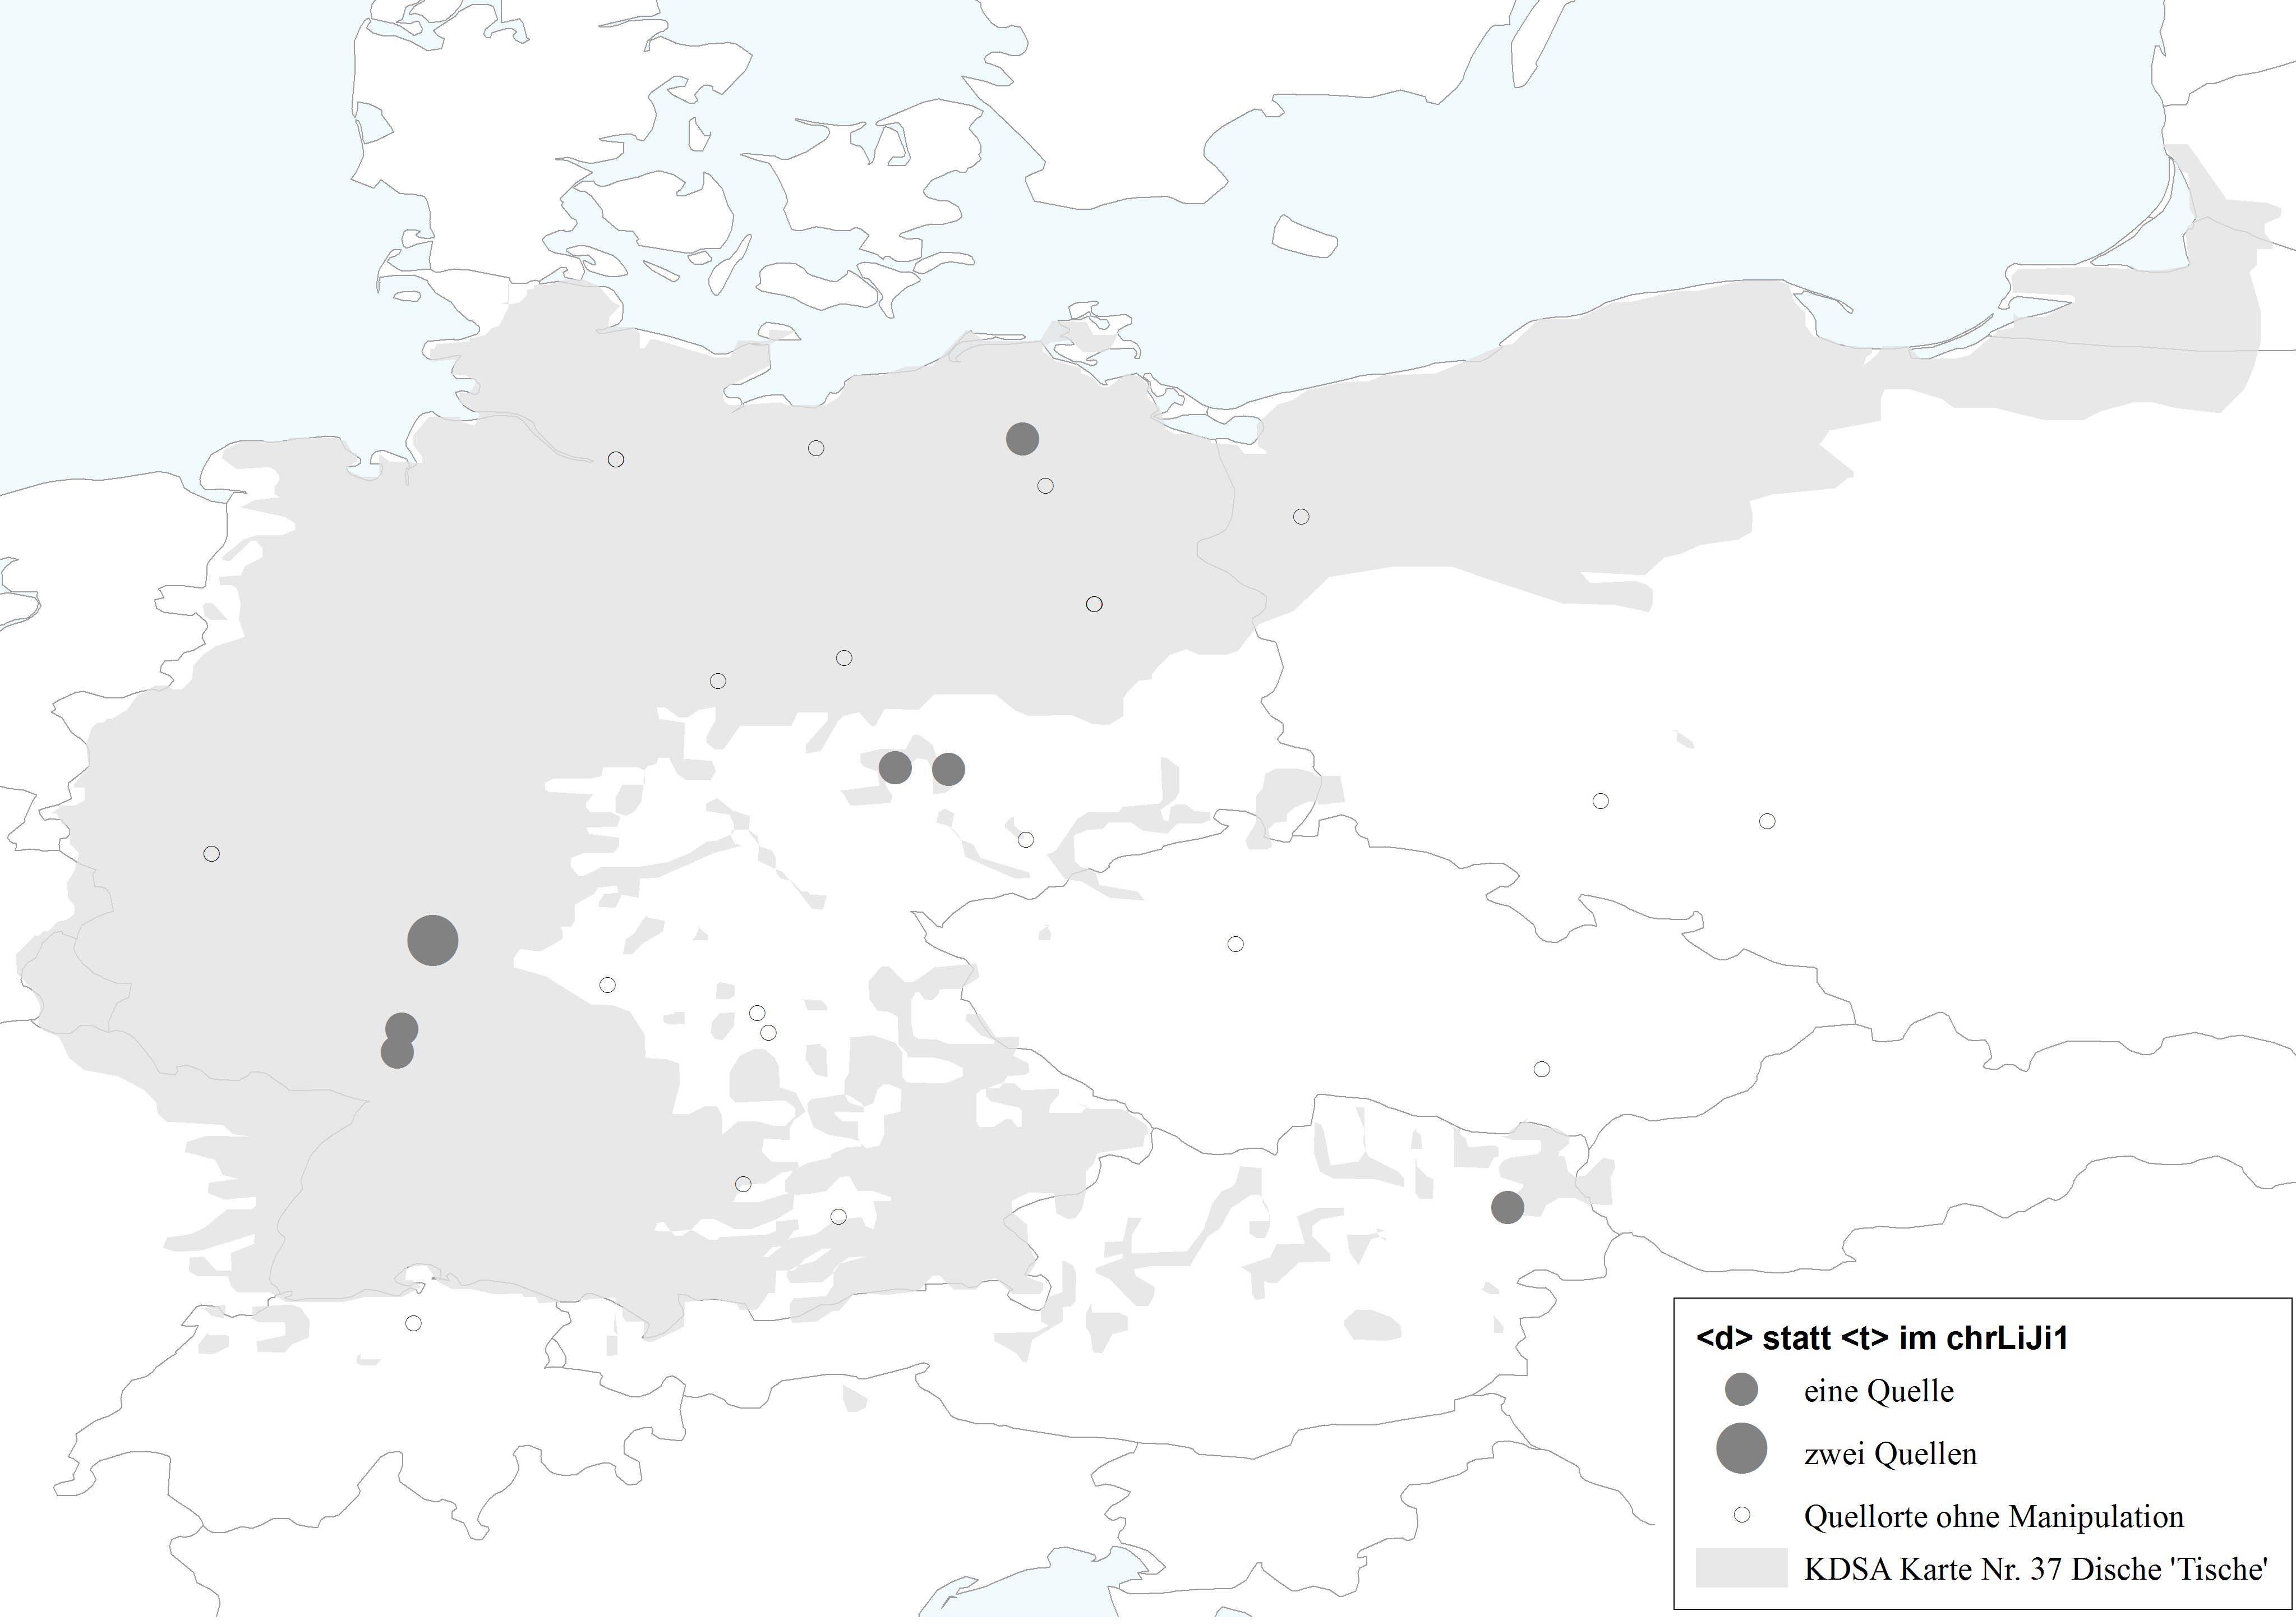
\includegraphics[scale=0.5]{figures/karte_dt_KDSA37.png}
		\caption{\label{kartedtkdsa} \isi{Lenisierung} von <d> im \hai{chrLiJi1} und den mod. dt. Dialekten (\hai{KDSA} Karte Nr. 37)}
		\end{figure}
\FloatBarrier




  
  \subsection{\isi{Lenisierung} und Fortisierung von /b/, /p/}\label{pb}

Vier Quellen des \hai{chrLiJi1} zeigen die Fortisierung von /b/ > /p/ im \isi{Anlaut} in der Schreibung von <p> statt <b> (s. Bsp. \ref{bsptpb1}–\ref{bsptpb4}). Die \isi{Lenisierung} von /p/ > /b/ als <b> statt <p> tritt in drei Quellen auf (s. Bsp. \ref{bsptbp1}–\ref{bsptbp3}).\\
 
  \eenumsentence{
 \item \textit{Puckelche} \sem{Buckel} (\hai{AJ} Berlin, 1825:\,6) \label{bsptpb1}
\item \textit{prav} \sem{brav} (\hai{BS} Mannheim, 1798:\,4; \hai{GW} n.a., ca. 1900:\,9)\label{bsptpb2}
%\item \textit{prav} \sem{brav} (\hai{GW} n.a., ca. 1900:\,9)\label{bsptpb3}
\item  \textit{Puckel} \sem{Buckel} (\hai{JP} Altona, 1867:\,50)\label{bsptpb4}



\item \textit{blerren} \sem{plerren, weinen} (\hai{OF}:\,2)\label{bsptbp1}
\item \textit{Bepier} \sem{Papier} (\hai{PG} Speyer, 1835:\,2)\label{bsptbp2}
\item \textit{Bolitik} \sem{Politik} (\hai{VD} Frankfurt, 1916:\,13),  \textit{Blatz} \sem{Platz} (\hai{VD} Frankfurt, 1916:\,18R)\label{bsptbp3}
  }
   
  
  Die Kartierung der Daten macht deutlich, dass die \isi{Lenisierung} nur im rheinfränkischen Raum (Frankfurt u. Speyer) auftritt (vgl. Abb. \ref{kartebpkdsa}). Im Niederdeutschen und auch in einer Mannheimer Quelle finden sich die Belege zur Fortisierung. Der Vergleich zur Situation in den deutschen Dialekten, zeigt, dass die Fortisierung besonders in den östlichen Siedlungsmundarten verbreitet ist (vgl. \hai{KDSA} Karte Nr. 3).  Die Fortisierung von /b/ > /p/ ist für das Elsässer \hai{SWJ} und \hai{SÜJ} bekannt (\cite[353,  356]{Bin-Nun1973}). Ob sie jedoch auch im \hai{NWJ} erfolgte, ist nicht bekannt.
  
  Im Rahmen der sog. binnendeutschen Konsonantenschwächung ist die \isi{Lenisierung} von /p/ > /b/  in einem Großteil der hochdeutschen Mundarten verbreitet, so auch im Rheinfränkischen, wo unsere relevanten Quellen liegen (vgl. \cite[330–346]{Schirmunski1962}; \cite[148f]{Koenig1978}). Nach \textcite[221]{Klepsch2004} haben auch die zu den entsprechenden deutschen Dialekten koterritorialen westjiddischen Dialekte an der Konsonantenschwächung teilgenommen. \textcite[298–303]{Timm1987} bestätigt dies für das Mitteljiddische insofern, als dass die weit verbreitete fehlende graphematische Homogenität zumindest für die Aufgabe des Fortis-Lenis-Kontrasts spreche. \\
   
  \begin{figure}[h!]
		\centering
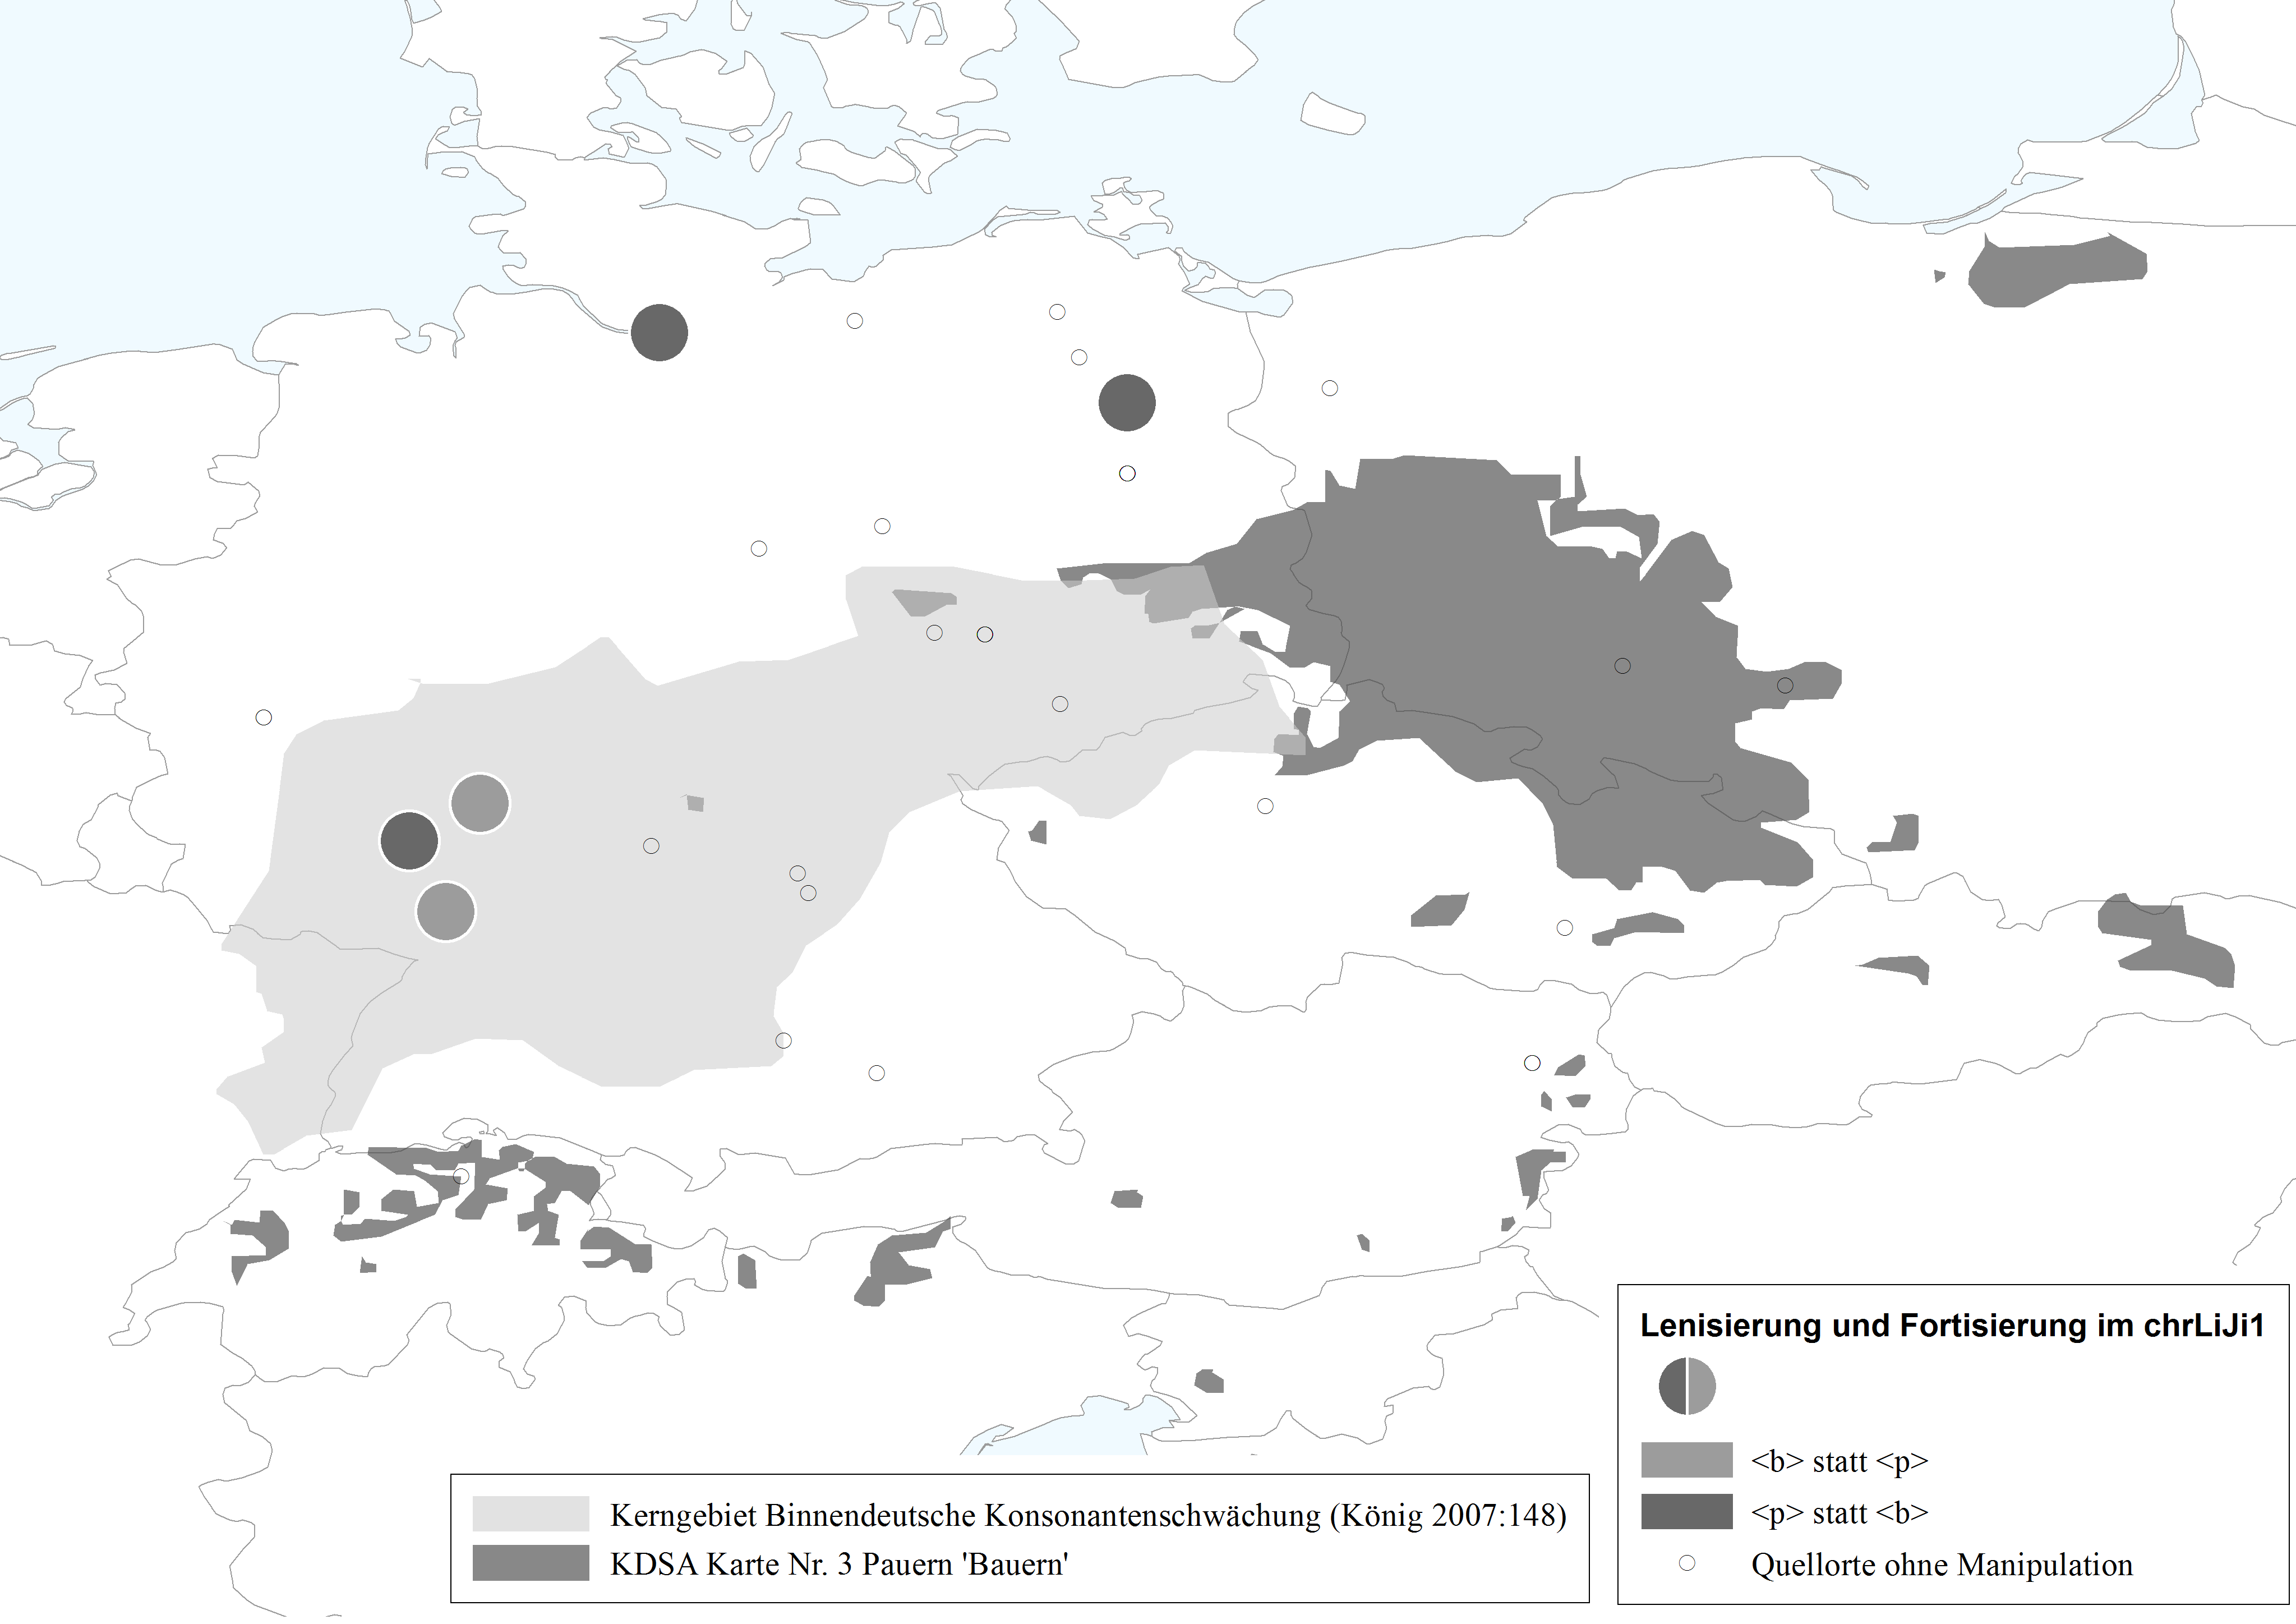
\includegraphics[scale=0.45]{figures/pb_kdsa.png}
		\caption{\label{kartebpkdsa} Graphien für <p> und <b> im \hai{chrLiJi1} mit \hai{KDSA} Karte Nr. 3 u. \textcite[148]{Koenig1978}}
		\end{figure}
\FloatBarrier
 
 %  \clearpage
 
Das \hai{jüdLiJi1} zeigt die Fortisierung in den zwei Berliner Pamphleten, s. \ref{bsppbliji2a}--\ref{bsppbliji2b}. Dies spricht dafür, dass die Fortisierungen im \hai{chrLiJi1} u.\,U. doch ein tatsächliches Phänomen des \hai{NWJ} einfangen.\\

  \eenumsentence{
\item \textit{praven} \sem{braven} (\hai{PBerlin1}:\,6) \label{bsppbliji2a}

\item \textit{Pauer} \sem{Bauer} (\hai{PBerlin2}:\,1.Sp.) \label{bsppbliji2b}
}

%Im \hai{LiJi2} finden sich weder Fortisierung noch \isi{Lenisierung} von /b/, /p/.


  
  \subsection{Fortisierung <g> als <k>}\label{kg}
%  %\noindent
Eine weitere Manipulation an Plosiven im \hai{chrLiJi1} ist die Fortisierung von /g/ als /k/ (vgl. \cite[330–346]{Schirmunski1962}). Diese findet sich in 13 Quellen des \hai{chrLiJi1} im  \isi{Anlaut} vor Konsonant und Vokal\footnote{Hier besonders im Partizipialpräfix \textit{ge-}.} (s. Bsp. \ref{bspkgliji1}–\ref{bspkgliji7}).

  \eenumsentence{
 \item \textit{klaich} \sem{gleich} (\hai{JK} Breslau, 1810\,35, 52, 57), \textit{Kriek} \sem{Krieg} (\hai{JK} Breslau, 1810:\,50) \label{bspkgliji1}
 \item  \textit{kewußt} \sem{gewusst} (\hai{DK} Osterwieck, 1872:\,47R)\label{bspkgliji2}
 \item \textit{kegen} \sem{gegen} (\hai{DW} Wien, 1773:\,66)\label{bspkgliji3}
 \item \textit{krauß} \sem{groß} (\hai{LR}:\,5)\label{bspkgliji4}
 \item  \textit{kehandelt} \sem{gehandelt} (\hai{PF} Augsburg, 1816:\,11), \textit{kewesen} \sem{gewesen} (\hai{PF} Augsburg, 1816:\,11, 12, 18), \textit{kesogt} \sem{gesagt} (\hai{PF} Augsburg, 1816:\,12), \textit{Keschmack} \sem{Geschmack} (\hai{PF} Augsburg, 1816:\,12, 13), \textit{kefunden} \sem{gefunden} (\hai{PF} Augsburg, 1816:\,12), \textit{kesehn} \sem{gesehen} (\hai{PF} Augsburg, 1816:\,12), \textit{keschlichen} \sem{geschlichen} (\hai{PF} Augsburg, 1816:\,12), \textit{keboten} \sem{geboten} (\hai{PF} Augsburg, 1816:\,12), \textit{kesagt} \sem{gesagt} (\hai{PF} Augsburg, 1816:\,14, 18), \textit{kedient} \sem{gedient} (\hai{PF} Augsburg, 1816:\,14), \textit{kescheidt} \sem{gescheit} (\hai{PF} Augsburg, 1816:\,18), \textit{kanz} \sem{ganz} (\hai{PF} Augsburg, 1816:\,18) \label{bspkgliji5}
 \item \textit{kraußen} \sem{großen} (\hai{TH} Merseburg, 1820:\,97) \label{bspkgliji6}
 \item \textit{kewaltik} \sem{gewaltig} (\hai{VD} Frankfurt, 1916:\,15),  \textit{keschrien} \sem{geschrien} (\hai{VD} Frankfurt, 1916:\,16) \label{bspkgliji7}

}


Daneben findet sich im \hai{chrLiJi1} die \isi{Auslautverhärtung}, d.\,h. die Fortisierung der Silbenkoda, von /g/ in drei Quellen graphematisiert (s. Bsp. \ref{bspkgliji8}–\ref{bspkgliji10}). Bemerkenswert daran ist, dass dieses Charakteristikum aller gesprochensprachlichen Varietäten des Deutschen wie auch des Jiddischen im Unterschied zu anderen konsonantischen Merkmalen nur in sehr wenigen Quellen auftaucht.\footnote{Zur \isi{Auslautverhärtung} im Jiddischen und Deutschen vgl. \textcite[373]{Bin-Nun1973}.} Scheinbar ist dem \hai{LiJi1} in erster Linie weniger an der Hervorhebung der gesprochenen Sprache als vielmehr an den Differenzen des Jiddischen zum Deutschen gelegen. \\

 \eenumsentence{
\item \textit{lebendik} \sem{lebendig} (\hai{JK} Breslau, 1810:\,44, 47), \textit{gesakt} \sem{gesagt} (\hai{JK} Breslau, 1810:\,6, 23, 30, 35, 37), \textit{schlaickt} \sem{schlägt} (\hai{JK} Breslau, 1810:\,26) \label{bspkgliji8}
\item \textit{gewaltik} \sem{gewaltig} (\hai{PA} Frankfurt, 1834:\,Titel, 11), \textit{Ufzück} \sem{Aufzüge} (\hai{PA} Frankfurt, 1834:\,Titel), \textit{zwanzik} \sem{zwanzig} (\hai{PA} Frankfurt, 1834:\,10), \textit{geduldik} \sem{geduldig} (\hai{PA} Frankfurt, 1834:\,10), \textit{sakt} \sem{sagt} (\hai{PA} Frankfurt, 1834:\,87W), \sem{gesagt} (\hai{PA} Frankfurt, 1834:\,16, 36, 114) \label{bspkgliji9}
\item  \textit{Keinik} \sem{König} (\hai{VD} Frankfurt, 1916:\,15, 18), \textit{wek} \sem{weg} (\hai{VD} Frankfurt, 1916:\,18R), \textit{fertik} \sem{fertig} (\hai{VD} Frankfurt, 1916:\,20), \textit{gewaltike} \sem{gewaltige} (\hai{VD} Frankfurt, 1916:\,14) \label{bspkgliji10}

}


Im \hai{KDSA} finden sich nur im Obersächsischen, wo die generelle Neutralisierung der Fortis und Lenis bei den Plosiven erfolgte \parencite[332]{Schirmunski1962}, Streubelege für die Fortisierung im \isi{Anlaut} in den deutschen Varietäten (vgl. Abb. \ref{kartekgkdsa}). Es muss jedoch berücksichtigt werden, dass die dem \hai{WA} wie dem \hai{KDSA} zugrundeliegenden Wenkermaterialien bei der Erhebung konsonantischer Daten nicht sehr ergiebig waren (vgl. \cite{Bremer1895}). Man kann daher davon ausgehen, dass die karierten Areale de facto weitaus größer sind, als die Daten vermuten lassen. Dennoch kann man in Karte \ref{kartekgkdsa} sehen, dass immerhin zwei Quellen im näheren Umfeld zur Fortisierung in den deutschen Mundarten liegen und dadurch beeinflusst sein können. Die übrigen Belege im westmitteldeutschen, bairischen und schlesischen Raum zu beurteilen fällt deutlich schwerer. Es ist möglich, dass dort in den deutschen Dialekten ebenfalls eine Fortisierung vorliegt, deren Interferenzen sich im \hai{LiJi1} niederschlagen oder aber, dass die Autoren durch diese Graphie eine \quein{Andersartigkeit} der jiddischen Dialekte darstellen wollen, die uns entweder nicht aus authentischen Quellen des Westjiddischen bekannt ist oder hier lediglich als literarisches Mittel fungiert, um \quein{Fremdheit} zu erzeugen.\\

  \begin{figure}[h!]
		\centering
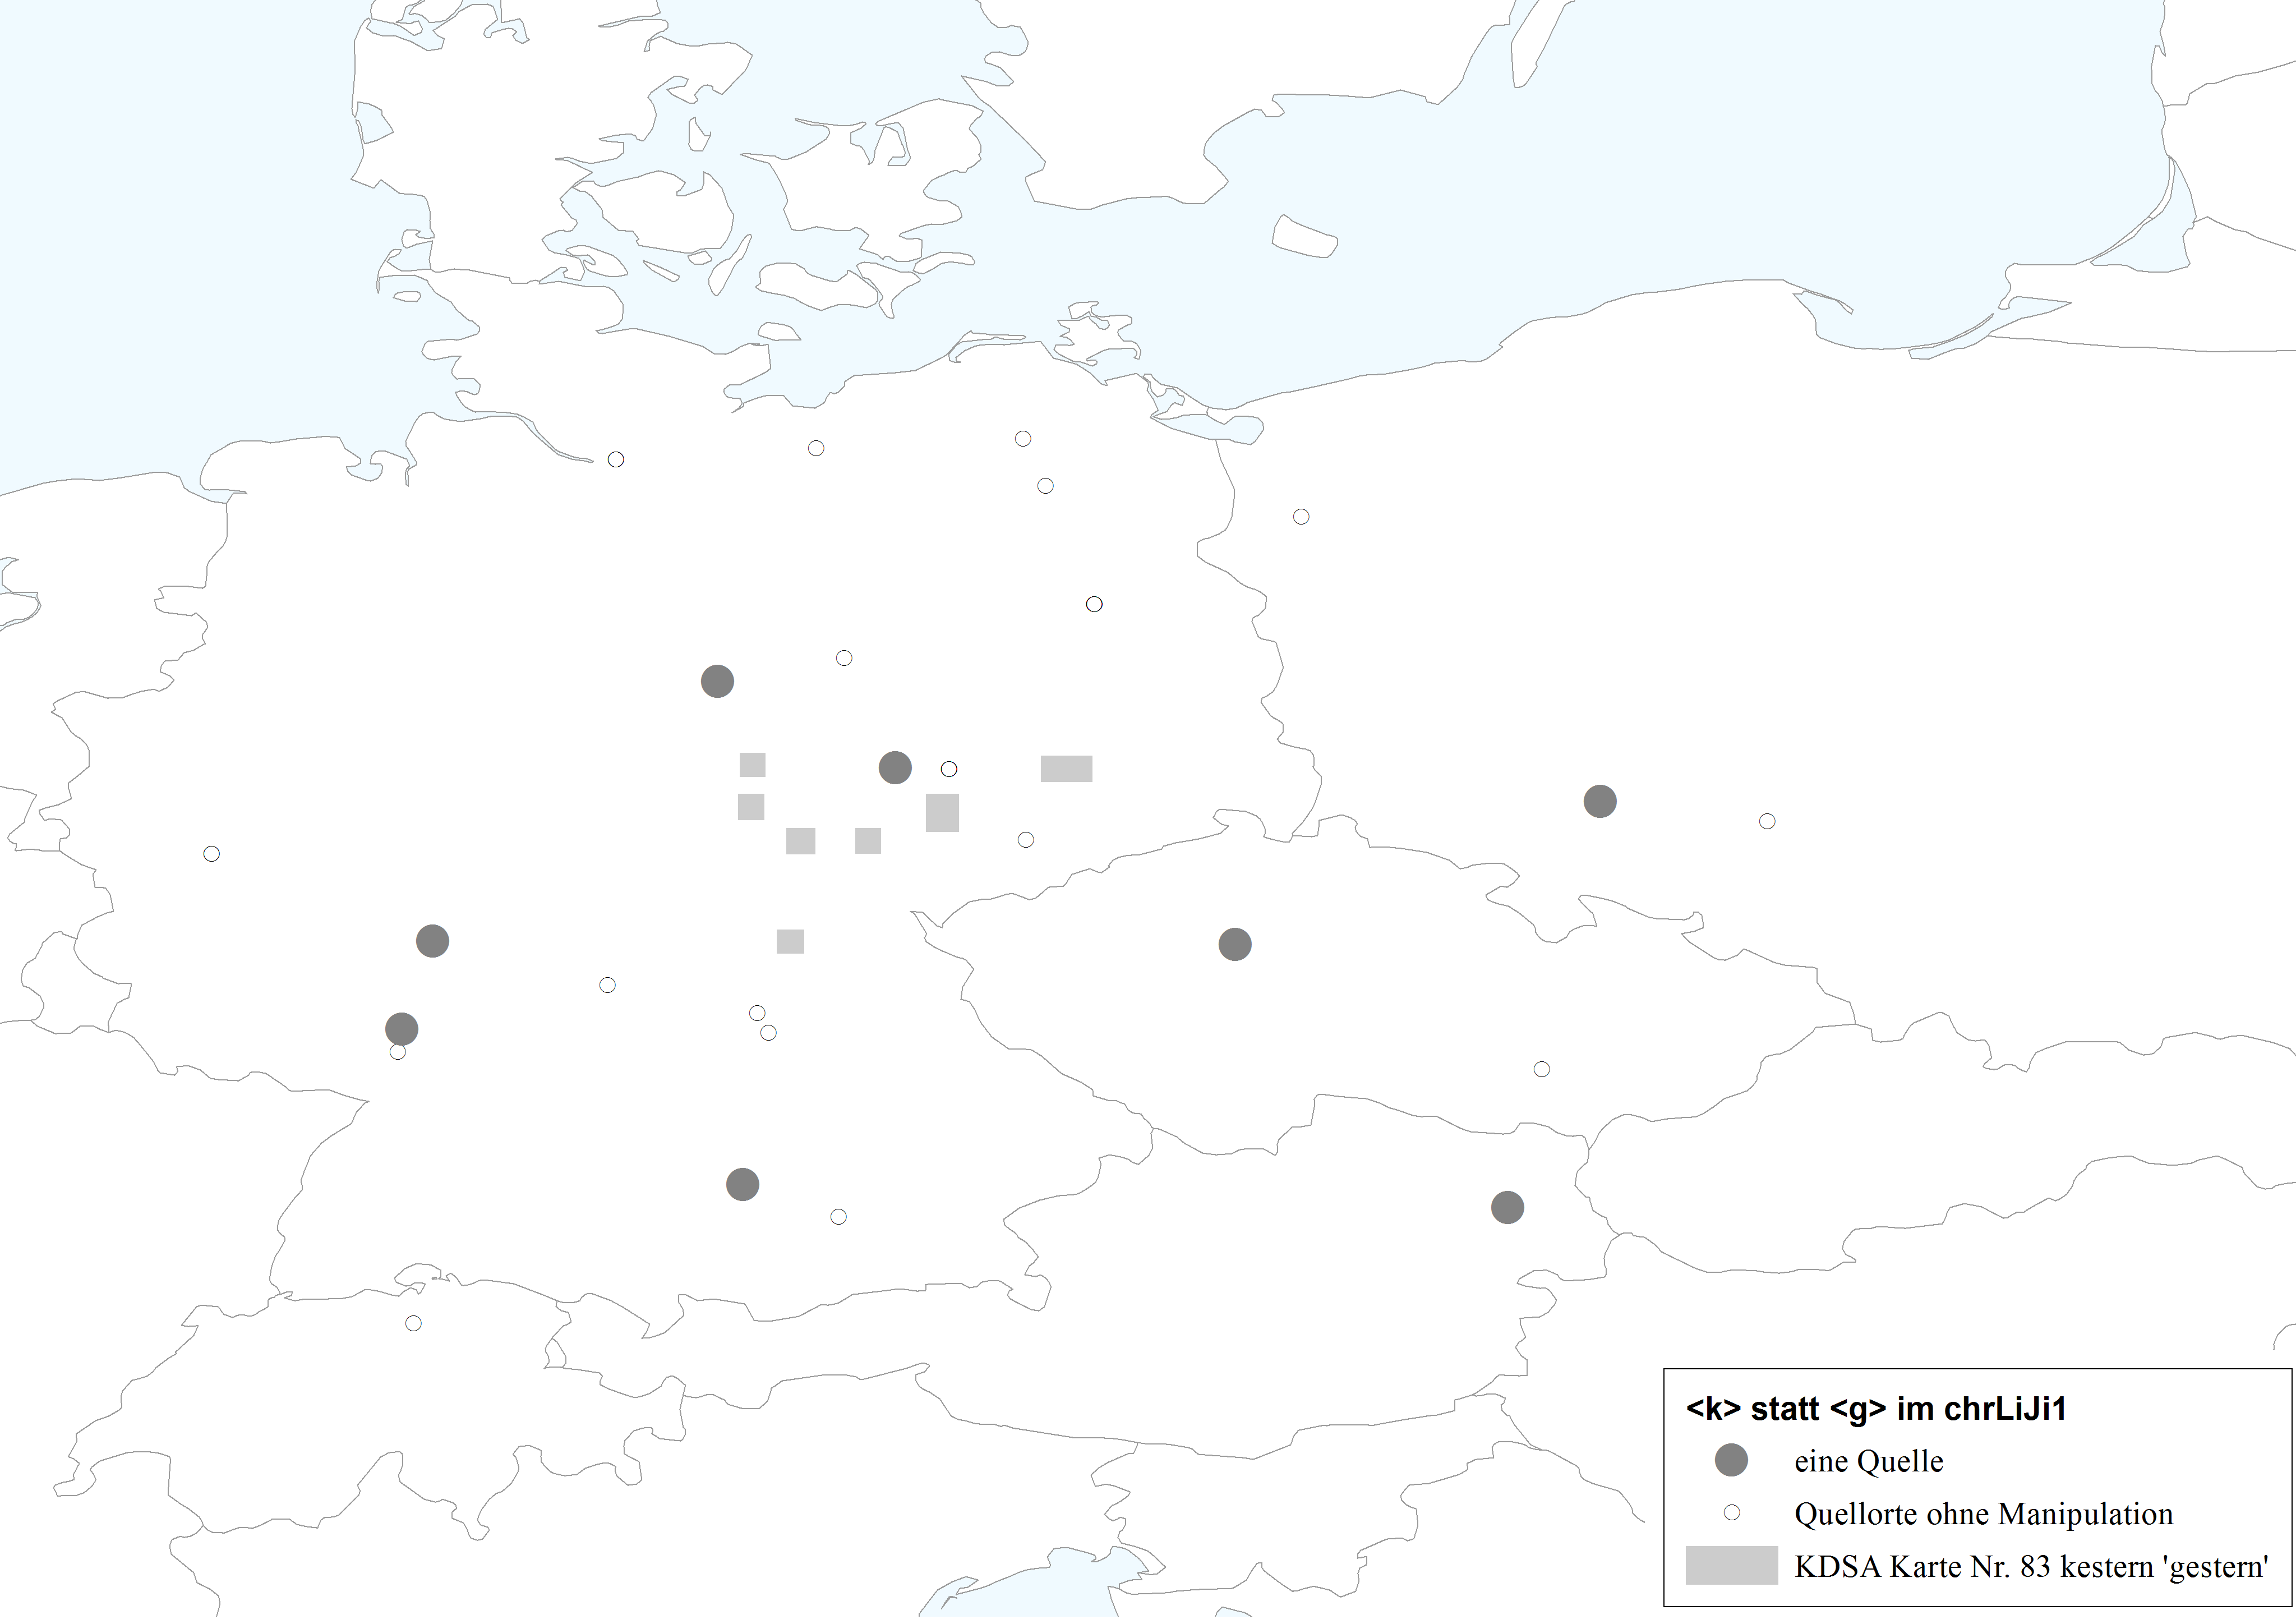
\includegraphics[scale=0.45]{figures/karte_kg_KDSA.png}
		\caption{\label{kartekgkdsa} <k> für <g> in \isi{Anlaut} im \hai{chrLiJi1} mit \hai{KDSA} Karte Nr. 83}
		\end{figure}
\FloatBarrier
		
		
Die tatsächliche Sprachsituation in den jiddischen Dialekten gestaltet sich wie folgt: Zwar zeigen einige wenige Wörter im modernen \hai{OJ} sogar eine solche Fortisierung, z.\,B. \RL{קעגן} \textit{kegn} \sem{gegen} (für weitere Bsp. s. \cite[373]{Bin-Nun1973}). Der einzige Beleg für eine Fortisierung von /g/ im \hai{jüdLiJi1} betrifft genau dieses Lexem: \textit{kegen} \sem{gegen} (\hai{PDebrecen}:\,4, 7), was damit eine ostjiddische Form korrekt wiedergibt. Die Regel ist jedoch im \hai{OJ} der Erhalt des Fortis–Lenis–Kontrastes.  So wird etwa das im \hai{LiJi} oftmals betroffene \textit{ge-}Präfix im Jiddischen immer als stimmhafter velarer Plosiv realisiert.  

Den Daten des \hai{LCAAJ} (Karte Nr. 83) zu Folge, liegt im \hai{ZWJ}, \hai{SWJ} und ndl. \hai{NWJ} mit der \isi{Lenisierung} von anlautendem /k/ > /g/ eine gegensätzliche Entwicklung vor (s. Karte \ref{kartekgkdsalcaaj}). Dies ist ein Reflex der sog. \quein{Binnendeutschen Konsonantenschwächung} und in nahezu allen hochdeutschen Dialekten anzutreffen (vgl. \cite[332]{Schirmunski1962}). Die \hai{LiJi}-Quellen bestätigen die westjiddische Situation des \hai{LCAAJ} jedoch nicht: eine \isi{Lenisierung} wird im \hai{LiJi} nirgends verschriftlicht.\\
		
		
		  \begin{figure}[h!]
		\centering
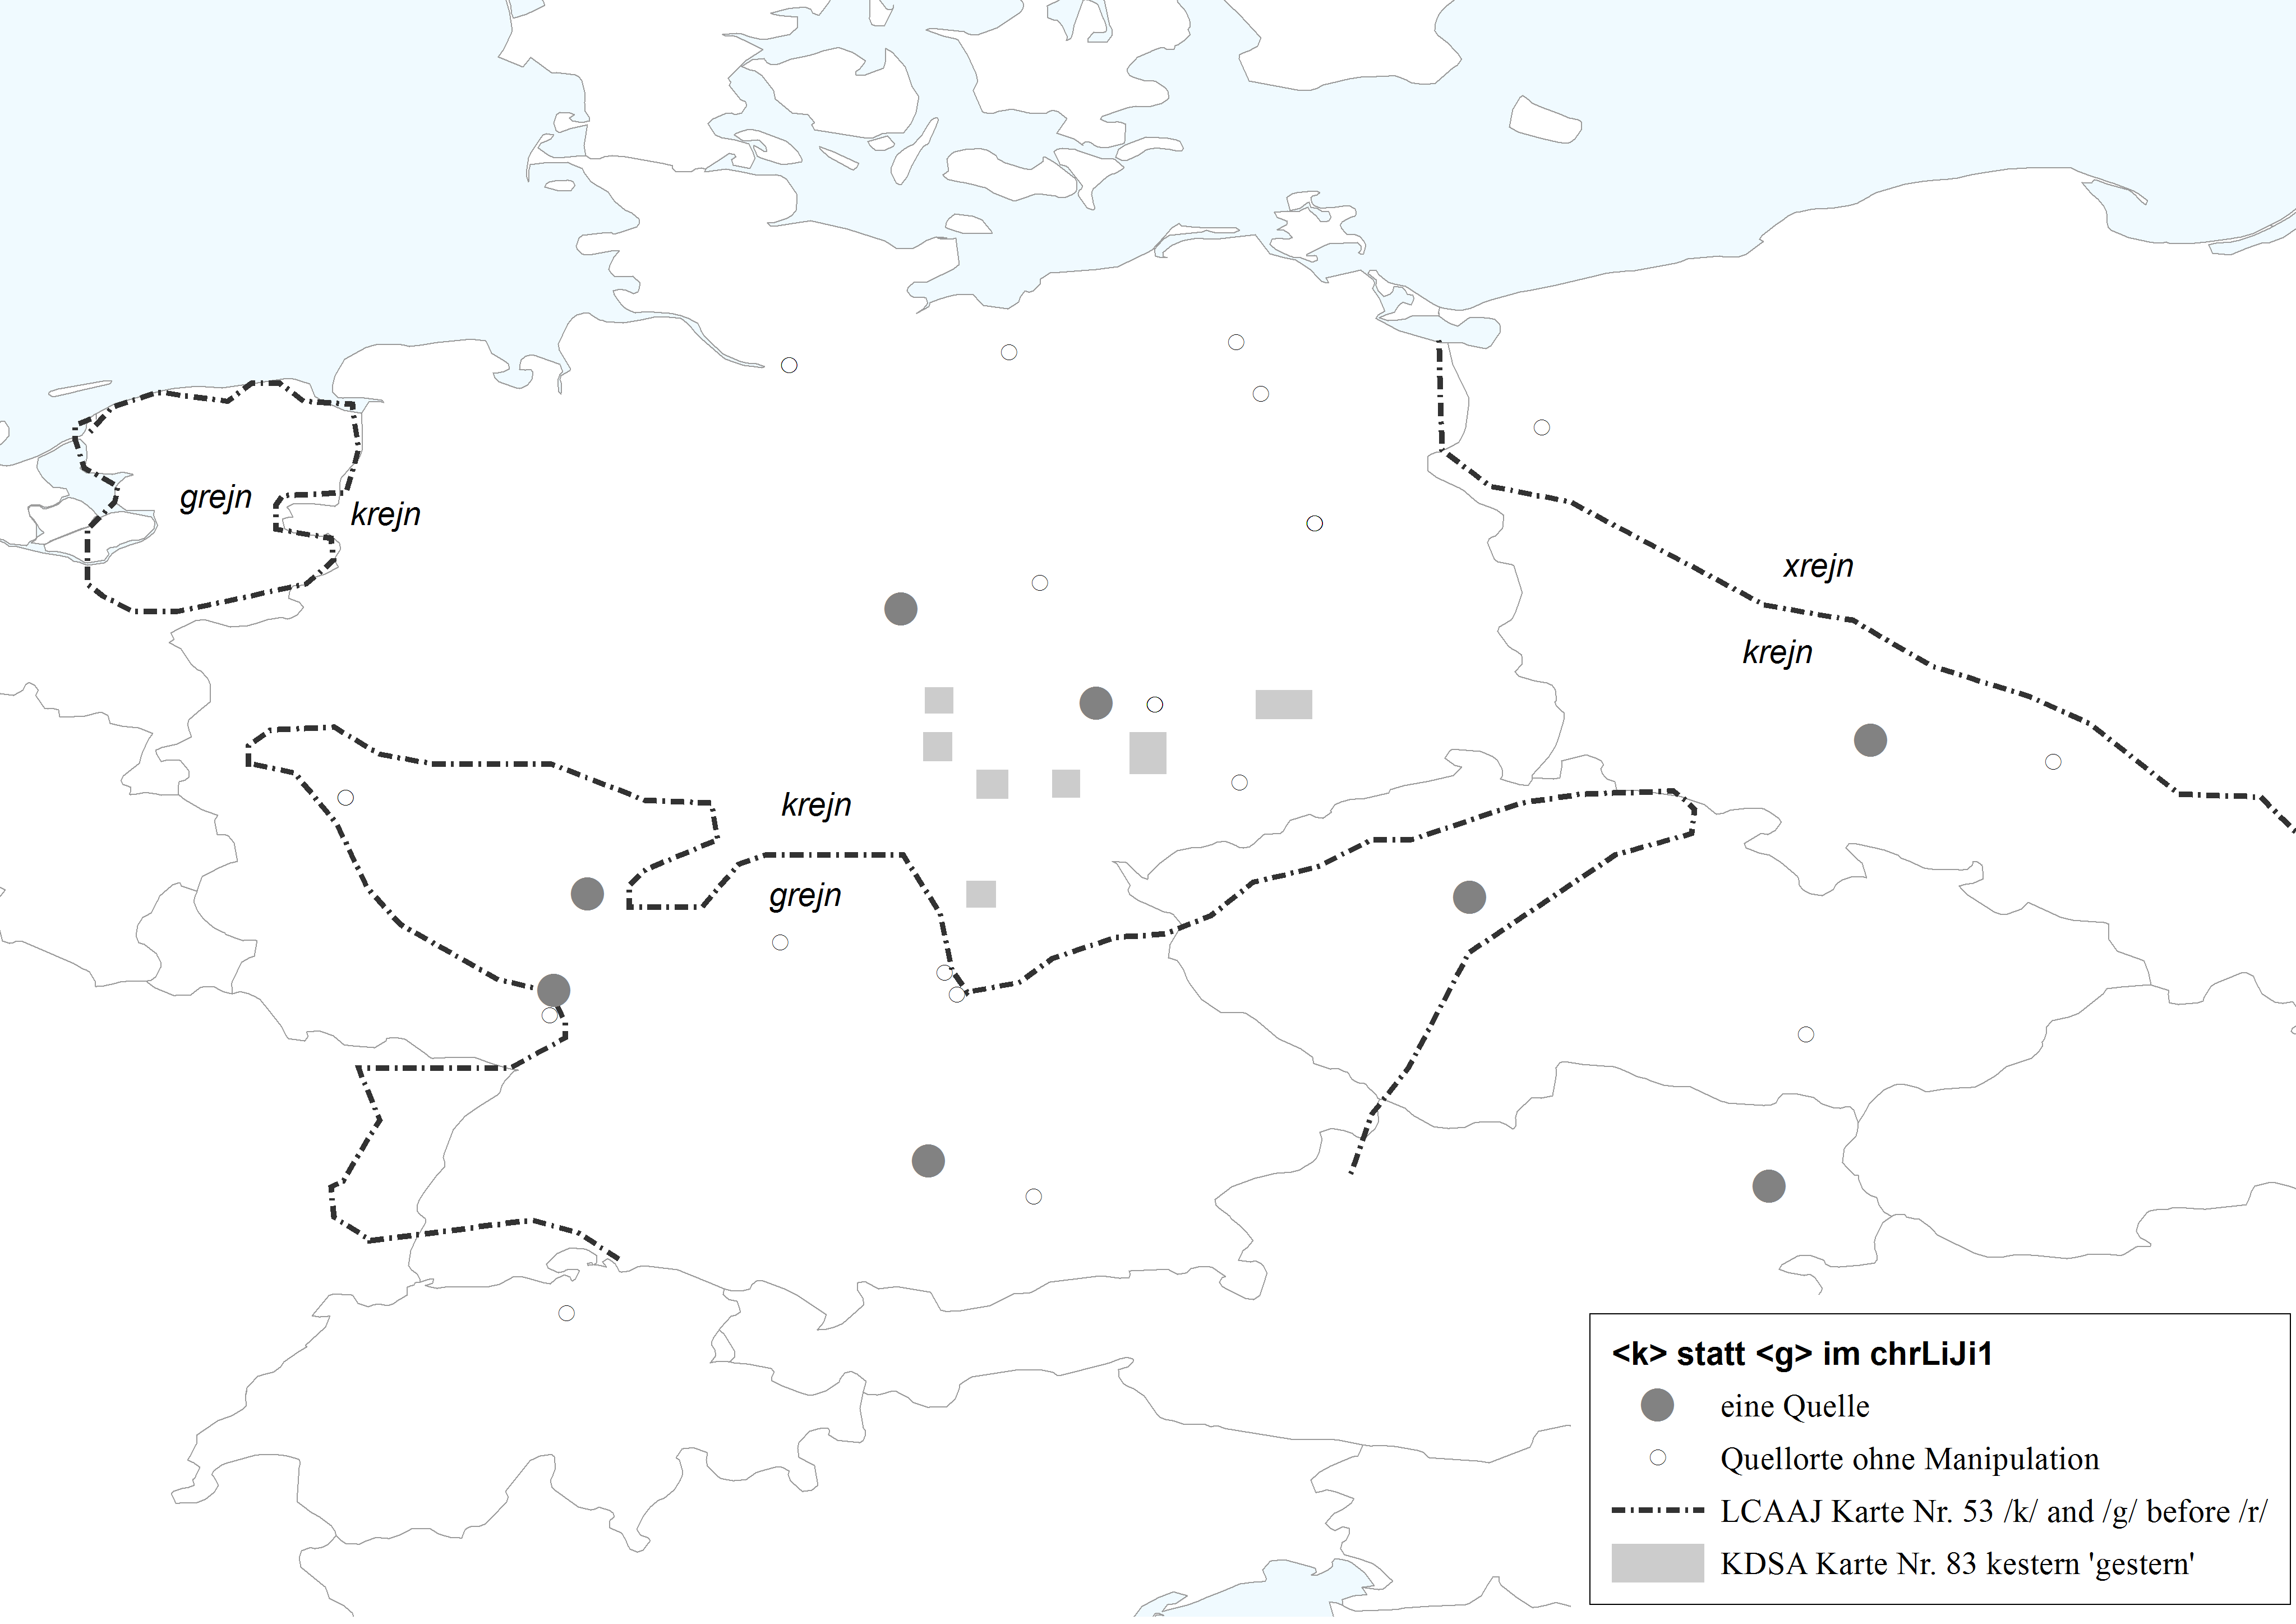
\includegraphics[scale=0.45]{figures/karte_kg_KDSA_lcaaj.png}
		\caption{\label{kartekgkdsalcaaj} <k> für <g> im \isi{Anlaut}  im \hai{chrLiJi1} mit \hai{KDSA} Karte Nr. 83 und \hai{LCAAJ} Karte Nr. 53}
		\end{figure}
\FloatBarrier


Eine sinnvolle Beurteilung der literaturjiddischen Belege einer Fortisierung von /g/ im \isi{Anlaut} ist letzten Endes nicht möglich, da übersichtliche Daten zur Situation des \isi{Konsonantismus} der deutschen und insbesondere der jiddischen Dialekte fehlen, die Rückschlüsse auf die Authentizität der literaturjiddischen Formen zulassen.\\
 
   \subsection{Lenisierungen und Fortisierungen als Reflex der oberdeutschen Medienverschiebung}
   %  %\noindent
  Eine mit der 2. \hai{LV} in Verbindung stehende Entwicklung der oberdeutschen Dialekte ist die sogenannte Medienverschiebung von ahd. /b/, /d/, /g/ zu /p/, /t/, /k/, die in althochdeutscher Zeit im vorwiegend alemannischen, bairischen und ostfränkischen Raum gewirkt hat (\cite[131–133]{Szczepaniak2007}). Allerdings ist die Medienverschiebung kein leicht zu fassendes Ereignis und vielfach unsystematisch durchgeführt worden bzw. rückgängig gemacht worden (vgl. \cite[131–133]{Szczepaniak2007}) und die Situation in den oberdeutschen Varietäten ist besonders mit Blick auf deren Diachronie weitestgehend ungeklärt.
 
 Die zuvor aufgezeigten Lenisierungen und Fortisierungen des \hai{chrLiJi1} zeigen dennoch deutliche Ähnlichkeit zu dieser oberdeutschen Entwicklung. Die areale Verteilung der potenziellen Belege der Medienverschiebungen zeigt kein klares Bild: zwar treten Medienverschiebungen gehäuft in Quellen aus dem oberdeutschen Raum auf, darüber hinaus aber auch recht häufig im Norden und Osten (z.\,T. auch Westen) des Untersuchungsgebiets (vgl. Karten in Abb. \ref{kartedtkdsa} S. \pageref{kartedtkdsa}, \ref{kartebpkdsa} S. \pageref{kartebpkdsa} u. \ref{kartekgkdsa} S. \pageref{kartekgkdsa}). Demnach ist nicht auszuschließen, dass die eigene Dialektalität der Autoren in diese Formen einfloss bzw. deren Konzept von oberdeutschen Dialekten, zu denen sie möglicherweise auch das Jiddische zählten.
 
 Doch die Formen des \hai{LiJi1} könnten auch auf einen tatsächlichen westjiddischen Sprachstand referieren. Vieles spricht dafür, dass die Medienverschiebung auch in den zum Oberdeutschen koterritorialen Dialekten des Westjiddischen stattgefunden hat (\hai{LCAAJ} Karte Nr. 53 vgl. Abb. \ref{kartekgkdsalcaaj} S. \pageref{kartekgkdsalcaaj}). Hierzu fehlt es jedoch noch an ausführlicheren Untersuchungen im Detail.\\
  
  %Besonders ahd. /d/ ist von der \isi{Lenisierung} besonders stark betroffen. 

  
  \subsection{Erhalt von westgerm. *-\textit{pp}-}
  %  %\noindent
Die in- und auslautende Geminate westgerm. *-\textit{pp}- blieb in Ost- und \ili{Westjiddisch} unverändert (\cite[189]{Kleine2008}; \cite[323–327]{Bin-Nun1973}). Im \hai{chrLiJi1} ist dies in drei Quellen korrekt umgesetzt (Bsp. \ref{bsp2lv1}–\ref{bsp2lv3}). Dabei liegen die Quellen \hai{FL} (Mannheim, 1778) und \hai{MV} (Berlin, 1862) im Gebiet, das die Entwicklung zu -\textit{pf}- nicht mitgemacht hat (vgl. \cite[64f]{Koenig1978}).\footnote{In einer dieser Quellen, die in den rheinfränkischen Raum verortet wurde, findet sich ein Beleg für unverschobenes germ. \textit{-k-} \textit{ick} \sem{ich} (\hai{FL} Mannheim, 1778:\,36), was keinem jiddischen (und auch keinem hochdeutschen) Dialekt entspricht und als einmaliger \quein{Fehler} zu bewerten ist.} Die Belege aus diesen Quellen könnten also auch auf Interferenzen mit den örtlichen deutschen Dialekten zurückgeführt werden. Es findet sich also nur eine Quelle (\hai{SV} München, 1890), bei der mit relativer Sicherheit eine authentische jiddische Form vorliegt.\\
  
   \eenumsentence{
 \item \textit{Kop} \sem{Kopf} (\hai{FL} Mannheim, 1778:\,38) \label{bsp2lv1}
 \item \textit{Köppe} \sem{Köpfe} (\hai{MV} Berlin, 1862:\,62, 153) \label{bsp2lv2}
 \item \textit{Knepp} \sem{Knöpfe} (\hai{SV} München, 1890:\,2), \textit{Koppe} \sem{Kopf} (\hai{SV} München, 1890:\,3, 5) \label{bsp2lv3}
  
} 

Im  \hai{jüdLiJi1} sind Belege für das Ausbleiben der 2. \hai{LV} bei westgerm. -\textit{pp}- deutlich häufiger. Sieben der zehn Quellen zeigen keine Affrikate (Bsp.\ref{bsp2lv4}–\ref{bsp2lv10}). Diese Quellen sind allesamt im Berliner Raum entstanden, womit Interferenzen mit den deutschen Dialekten nicht auszuschließen sind (vgl. \cite[64f]{Koenig1978}). 
 
  \eenumsentence{
\item \textit{Strümp} \sem{Strümpfe} (\hai{GuS1}:\,3), \textit{ausgestoppt} \sem{ausgestopft} (\hai{GuS1}:\,4), \textit{Kopp} \sem{Kopf} (\hai{GuS1}:\,4) \label{bsp2lv4}

\item  \textit{Köppe} \sem{Köpfe} (\hai{GuS5}:\,4), \textit{gehuppt} \sem{gehüpft} (\hai{GuS5}:\,4), \textit{kuppernen} \sem{kupfernen} (\hai{GuS5}:\,5) \label{bsp2lv5}

\item \textit{Kopp} \sem{Kopf} (\hai{GuS10}:\,6, 9, 10, 11), \textit{Schulklopper} \sem{Schulklopfer} (\hai{GuS10}:\,9, 11), \textit{Kupperhütchens} \sem{Kupferhüten} (\hai{GuS10}:\,10, 11) \label{bsp2lv6}

\item   \textit{zerkloppt} \sem{zerklopft} (\hai{GuS15}:\,3R), \textit{vollgestoppt} \sem{vollgestopft} (\hai{GuS15}:\,3R) \label{bsp2lv7}

\item \textit{Kopp} \sem{Kopf} (\hai{GuS23}:\,9) \label{bsp2lv8}

\item \textit{Tröppcher} \sem{Tropfen} (\hai{PBerlin1}:\,2), \textit{Kopp} \sem{Kopf} (\hai{PBerlin1}:\,4, 6, 7) \label{bsp2lv9}

\item \textit{Kopp} \sem{Kopf} (\hai{PBerlin2}:\,1.Sp.), \textit{Schtrümps/Schtrümpe} \sem{Strümpfe} (\hai{PBerlin2}:\,1.Sp., 2.Sp.) \label{bsp2lv10}
}


Wie auch die \isi{Auslautverhärtung} ist dieses, orthographisch relativ leicht umsetzbare Phänomen erstaunlich selten im \hai{chrLiJi1} zu finden. Auffallend häufiger sind hingegen Belege im \hai{jüdLiJi1}. In den meisten Fällen stammen die Quellen aus dem sich zwischen Benrather- und Speyrer-Linie befindenden Areal, in dem die 2. \hai{LV} an dieser Position wie im Jiddischen unterlassen wurde. \\




\subsection{Spirantisierung <b> als <w>}\label{bw}
%  %\noindent  
Die Spirantisierung von (insbes. intervokalisch) /b/ > /v/ hat große Teile des deutschen Sprachgebiets erfasst (\hai{KDSA} Karten Nr. 23–33, bes. 30). Neben dem Niederdeutschen, wo westgerm. \textit{ƀ} *[v] unverschoben blieb, findet  sich die Spirantisierung im gesamten Westmitteldeutschen, Niederalemannischen, im Nordbairischen Böhmens und vereinzelt im Mittel- und Südbairischen. Im bairischen Raum ist sie seit dem Mittelhochdeutschen schriftlich belegt (\hai{DWB}: \citeyear[Bd. 27, Sp. 4]{DeutschesWB}).  \textcite[328, 357]{Bin-Nun1973} stellt fest, dass diese Spirantisierung im Jiddischen nur in einzelnen Lexemen und regional gebunden auftritt (Bsp. \ref{bspOJbw1}–\ref{bspOJbw3}). \textcite[357]{Bin-Nun1973} geht bei diesem Phänomen von Einflüssen aus den koterritorialen deutschen Dialekten aus.\\

 \eenumsentence{
\item Standard oj. \RL{אָוונט} \textit{ovnt} \sem{Abend} \label{bspOJbw1}
\item oj. Dialekte \textit{oiwm} \sem{oben}  \parencite[356]{Bin-Nun1973}; Standard oj. \RL{איבער} \textit{iber} \label{bspOJbw2}
\item Elsässer wj. \textit{lîwi} \sem{liebe} \parencite[356]{Bin-Nun1973}; Standard oj. \RL{ליבער} \textit{liber}\label{bspOJbw3}
}

Die Verbreitung der Spirantisierung im \hai{Westjiddischen} erfasst nach Beranek (\hai{WjSA}: Karte Nr. 33) nur ein kleines Gebiet im äußersten Westen des \hai{ZWJ} und \hai{SWJ}. Spätere Ausbreitungen dieser Form auf östliche Varietäten des \hai{WJ} werden hier jedoch auch (durch diffuse Pfeile angedeutet) angenommen. Der \hai{LCAAJ} (Karte Nr. 51) setzt ein deutlich größeres Areal im westlichen \hai{WJ} an (vgl. Abb. \ref{kartebwlcaaj}). Dieses Areal entspricht weitestgehend der Verbreitung dieses Phänomens in den deutschen Mundarten (\hai{KDSA} Karten Nr. 23–33, bes. 30). \citeauthor{Bin-Nun1973}s (\citeyear[357]{Bin-Nun1973}) Hypothese eines deutschen Einflusses auf das Jiddische ist zumindest im \hai{WJ} nicht auszuschließen.
  
Im \hai{chrLiJi1} finden sich lediglich zwei Quellen, die sich der Spirantisierung als Markierungsmittel bedienen (\ref{bspLiJibw1}–\ref{bspLiJibw4}). Diese liegen im bzw. nahe dem Gebiet, für das der \hai{LCAAJ} die Spirantisierung verzeichnet (vgl. Abb. \ref{kartebwlcaaj}). Für das \hai{jüdLiJi1}, dessen Quellen im östlichen \hai{WJ} liegen, ist nur ein singulärer Beleg in der westlichsten aller Quellen zu finden (Bsp. \ref{bspLiJibw3}).\\ 

 \eenumsentence{
\item \textit{nowel} \sem{nobel} (\hai{SV} München, 1890:\,3) \label{bspLiJibw1}
\item \textit{hewe} \sem{haben} (\hai{VD} Frankfurt, 1916:\,14, 15, 17, 18, 20), \textit{iweraal} \sem{überall} (\hai{VD} Frankfurt, 1916:\,15, 18), \textit{begewe} \sem{begeben} (\hai{VD} Frankfurt, 1916:\,15R, 20R),  \textit{derneewe} \sem{daneben} (\hai{VD} Frankfurt, 1916:\,15R),  \textit{iwle} \sem{übler} (\hai{VD} Frankfurt, 1916:\,21),  \textit{verreiwe} \sem{verreiben} (\hai{VD} Frankfurt, 1916:\,22R),  \textit{schreiwe} \sem{schreiben} (\hai{VD} Frankfurt, 1916:\,22R), \textit{liewender} \sem{liebender} (\hai{VD} Frankfurt, 1916:\,22) \label{bspLiJibw2}
\item \textit{Struwelpeter} \sem{Strubbelpeter} (\hai{PAlsleben}:\,Titel) \label{bspLiJibw3}
\item \textit{uwnt} \sem{Abend} (\hai{WWR}:\,14, 29, 66, 20, 76, 112, 130, 144, 146) \label{bspLiJibw4} 
 }
 
		  \begin{figure}[h!]
		\centering
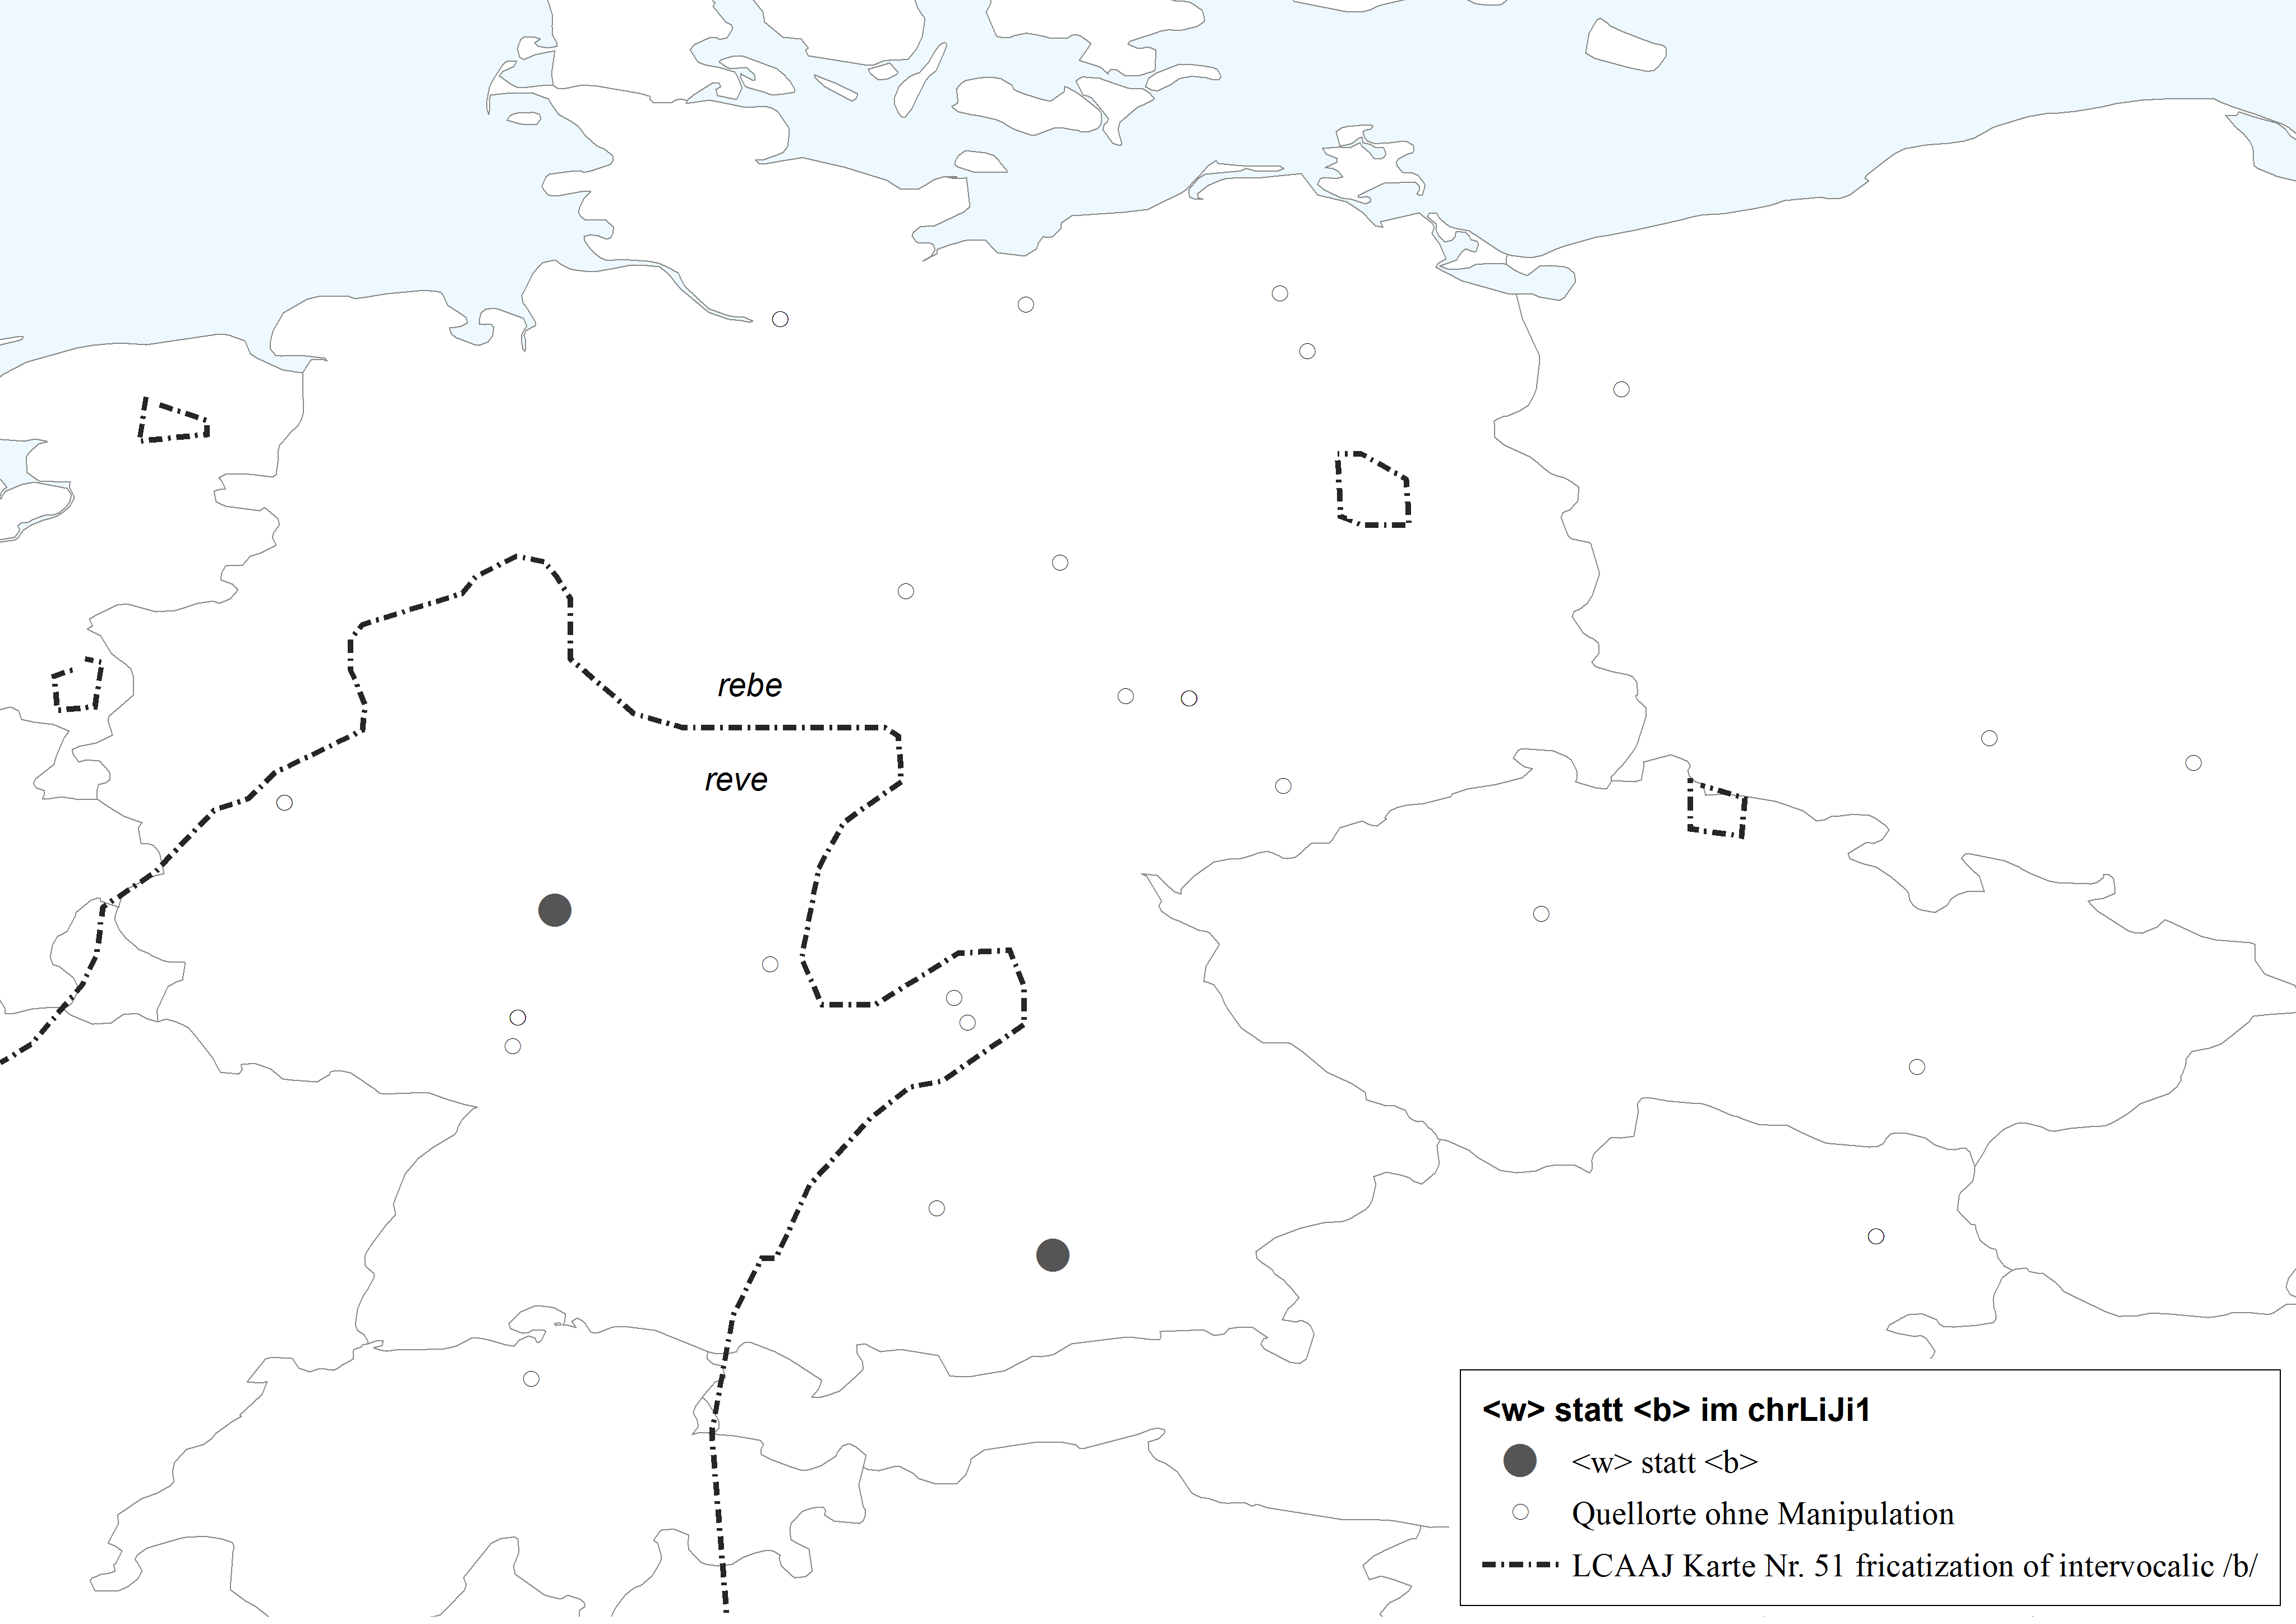
\includegraphics[scale=0.1]{figures/karte_bw_lcaaj51_vers2_2.png}
		\caption{\label{kartebwlcaaj} <w> für <b> im \hai{chrLiJi1} mit \hai{LCAAJ} Karte Nr. 51}
\end{figure}
\FloatBarrier
		

  \section{Diachrone und diatopische Verteilung phonologischer Manipulationen}\label{fazitphon}
 
%\noindent
 
 Von den insgesamt 26\footnote{Ausgenommen wurde hier die Hyperkorrektur von mhd. \textit{î} (\hai{V34}) als <a>, <ah>, <aa>, da es sich hierbei um eine sekundäre Interferenz mit der Monophthongierung von mhd. \textit{ei} (V24) handeln kann (oder aber auch eine zentralostjiddische Form darstellen kann). Einzeln Eingang in die Zählung haben hingegen die Zusammenfälle von \hai{V24} und \hai{V44} und von mhd. \textit{ê} und \textit{œ} gefunden.} untersuchten phonologischen Strategien des \hai{chrLiJi1} werden in einer Quelle (\hai{VD} Frankfurt, 1916) maximal 17 eingesetzt (vgl. Tabelle \ref{tblphonall}). Der Mittelwert beträgt 6,78 (Standardabweichung 4,15) Phänomene pro Quelle. Dies ist ein erstaunlich hoher Durchschnitt; besonders im Vergleich mit der Lexik, die eine vergleichsweise geringe Rolle im \hai{chrLiJi1} spielt. \\
  
  \begin{table}[h!]
\centering
		\begin{tabular}{lc}
		\hline
	\textbf{Quellen} & \textbf{phon. Phänomene} \\  \hline
 \hai{VD} & 17 \\
\hai{SV} & 16\\
\hai{TH}, \hai{MV} & 14\\
\hai{PA} & 13\\
\hai{GW } & 12\\
 \hai{PF}, \hai{AJ} & 11\\
\hai{SS}, \hai{DW},  \hai{AD}, \hai{MS}, \hai{AK} &10\\
\hai{JP},  \hai{PG}, \hai{JK}, \hai{FE} & 9\\
\hai{DG}, \hai{NW}, \hai{AO}  & 8\\
\hai{GP}, \hai{AT}, \hai{BW}, \hai{WA} & 7\\
\hai{UT}, \hai{DK},  \hai{LM}, \hai{FL}, \hai{OF}, \hai{PM}, \hai{IA}, \hai{LS}  & 6\\
\hai{LB}, \hai{EJ}, \hai{DP}  & 5\\
\hai{PL}, \hai{HJ} & 4\\
\hai{LR} & 3\\
\hai{VE}, \hai{AH},  \hai{BS}, \hai{FS}, \hai{EV}, \hai{PP}, \hai{BP} & 2\\
\hai{SB}, \hai{LP}, \hai{FM}, \hai{SH}, \hai{JD} &1\\ \hline
  
  
  	
  \end{tabular} 
		 \caption{Anzahl phonologischer Manipulationen im \hai{chrLiJi1}}
		 \label{tblphonall}
		 \end{table}  
  


Das Diagramm in Abbildung \ref{phonall} zeigt, wie viele phonologische Phänomene pro Quelle eingesetzt werden. Quellen mit besonders vielen phonologischen Markierungen finden sich dabei zwischen 1820 und 1830. Aber auch einige der späteren Quellen ab 1890 zeichnen sich durch eine besondere Vielfalt phonologischer Manipulationen aus.\\
 
 %großes histogramm
\begin{figure}[h!]
	\begin{tikzpicture}
		\begin{axis}[width=1.02\textwidth,height=0.2\textheight,
		legend style={at={(1,1)},xshift=+0.2cm, yshift=-0cm,anchor=north west,nodes=left},
			%title={Funktionstypen des sp\"aten Westjiddisch},
			xtick={1700, 1725, 1750, 1775, 1800, 1825, 1850, 1875, 1900, 1925, 1950, 1975}, ytick=,
			x tick label style={/pgf/number format/1000 sep=}, 
			y tick label style={/pgf/number format/1000 sep=},
			%extra y ticks={456.1, 1022.4},
			%extra y tick labels={{456,1},{1022,4}},
			extra y tick style={grid=major,
				tick label style={, ,}},
				ymin=0.7,
				ymax=19.1,
			ylabel={Phänomene},
			enlarge x limits=0.03]	
	
			
\addplot [thick] table [x=jahr, y=SUMME] {figures/ALLE_summe1_dia.txt}; %1


		\end{axis}
	\end{tikzpicture}
	\caption{Quantität phonologischer Markierungen im \hai{chrLiJi1}}
	\label{phonall}	
\end{figure}
\FloatBarrier
 
 
 Vier\footnote{Dabei handelt es sich um die Monophthongierungen von \hai{V24} und \hai{V44} zu /a\textlengthmark/, sowie deren \isi{Zusammenfall} und die Diphthongierung von \hai{V42} zu /au/, /ou/.} für das Westjiddische charakteristische phonologische Eigenschaften werden von elf Quellen eingesetzt; acht Quellen hingegen zeigen keines dieser Phänomene. Der Mittelwert liegt hier bei 2,37 (1,17 Standardabweichung) Phänomenen pro \hai{chrLiJi1}-Quelle. Wie die Verteilung in \ref{phonwjall} zeigt, ist weder eine Abnahme westjiddischer Phänomene im Verlauf des 19. Jahrhunderts zu verzeichnen, noch eine Phase erkennbar in der westjiddische Formen im \hai{chrLiJi1} präsenter sind als sonst. Es ist zwischen 1800 und 1875 eine generell hohe Dichte an authentisch westjiddischen phonologischen Phänomenen festzustellen, deren geringer Schwund nach 1875 vorwiegend der fehlenden Korpusdichte im letzten Drittel des 19. Jahrhunderts geschuldet ist. Ab 1875 finden sich verhältnismäßig weniger Quellen, die diese authentischen Phänomene belegen. Man könnte dies auch generell damit in Verbindung setzen, dass ab dieser Zeit \ili{Westjiddisch} nur mehr marginal in der deutschen Sprachlandschaft präsent war.\\  
 
 
 %großes histogramm wj
\begin{figure}[h!]
	\begin{tikzpicture}
		\begin{axis}[width=1.02\textwidth,height=0.2\textheight,
		legend style={at={(1,1)},xshift=+0.2cm, yshift=-0cm,anchor=north west,nodes=left},
			%title={Funktionstypen des sp\"aten Westjiddisch},
			xtick={1700, 1725, 1750, 1775, 1800, 1825, 1850, 1875, 1900, 1925, 1950, 1975}, ytick=,
			x tick label style={/pgf/number format/1000 sep=}, 
			y tick label style={/pgf/number format/1000 sep=},
			%extra y ticks={456.1, 1022.4},
			%extra y tick labels={{456,1},{1022,4}},
			extra y tick style={grid=major,
				tick label style={, ,}},
				ymin=0.7,
				ymax=4.8,
			ylabel={Phänomene},
			enlarge x limits=0.03]	
	
			
\addplot [thick] table [x=jahr, y=wj_all_phon] {figures/phon_wj_dia.txt}; %1


		\end{axis}
	\end{tikzpicture}
	\caption{Quantität \textit{korrekt} imitierter westjiddischer phonologischer Markierungen im \hai{chrLiJi1}}
	\label{phonwjall}	
\end{figure}
\FloatBarrier
 

Insbesondere die vokalischen Manipulationen treten gemeinsam und über den untersuchten Zeitraum hinweg kontinuierlich auf, wie das Streudiagramm in Abb. \ref{phonwjallstreu} zeigt. Konsonantische Phänomene hingegen kommen besonders im \hai{chrLiJi1} ab der zweiten Hälfte des 19. Jahrhunderts auf. So sind die Quellen zwischen 1840 und 1875 besonders vielfältig bezüglich der phonologischen Markierung. Die kartographische Darstellung in Abb. \ref{karteplosive} zeigt, dass konsonantische Manipulationen neben dem rheinfränkischen Raum, wo die entsprechenden Phänomene auch in den örtlichen deutschen Dialekten verbreitet sind, besonders häufig im (Nord-)Osten auftauchen. Dies betrifft insbesondere die späteren Quellen. \\


 \begin{figure}[h!]
	

	\begin{tikzpicture}

		\begin{axis}[only marks, width=0.82\textwidth,height=0.68\textheight,
		legend style={at={(1,1)},xshift=+0.2cm, yshift=-0cm,anchor=north west,nodes=left},
			%title={Funktionstypen des sp\"aten Westjiddisch},
			xtick={1700, 1725, 1750, 1775, 1800, 1825, 1850, 1875, 1900, 1925, 1950, 1975}, ytick=\empty,
			x tick label style={/pgf/number format/1000 sep=}, 
			y tick label style={/pgf/number format/1000 sep=},
			%extra y ticks={456.1, 1022.4},
			%extra y tick labels={{456,1},{1022,4}},
			extra y tick style={grid=major,
				tick label style={, ,}},
				ymin=0.51,
				ymax=24.9,
			ylabel={Phänomene},
			enlarge x limits=0.03]	
\addplot [mark=*, Fuchsia] table [x=jahr, y=wb] {figures/all_wb_24.txt}; \addlegendentry{<w> statt <b>}
\addplot [mark=*, BrickRed] table [x=jahr, y=LVp] {figures/all_LVp_23.txt}; \addlegendentry{germ. -\textit{pp}-}
\addplot [mark=*, MidnightBlue] table [x=jahr, y=kg] {figures/all_kg_22.txt}; \addlegendentry{<k> statt <g>}
\addplot [mark=*, black] table [x=jahr, y=bp] {figures/all_bp_21.txt}; \addlegendentry{<b> statt <p>}
\addplot [mark=*, Thistle] table [x=jahr, y=pb] {figures/all_pb_20.txt}; \addlegendentry{<p> statt <b>}
 \addplot [mark=*, LimeGreen] table [x=jahr, y=td] {figures/all_td_19.txt}; \addlegendentry{<t> statt <d>}
\addplot [mark=*, ProcessBlue] table [x=jahr, y=dt] {figures/all_dt_18.txt}; \addlegendentry{<d> statt <t>}
\addplot [mark=*, Maroon] table [x=jahr, y=s] {figures/all_s_z_17.txt}; \addlegendentry{<s> statt <z>}
\addplot [mark=*, Melon] table [x=jahr, y=sz] {figures/all_sz_z_16.txt}; \addlegendentry{<ß> statt <z>}
 \addplot [mark=*, RoyalPurple] table [x=jahr, y=scht_anlaut] {figures/all_scht_an_15.txt}; \addlegendentry{<scht> (\isi{Anlaut})}
\addplot [mark=*, YellowGreen] table [x=jahr, y=scht_auslaut] {figures/all_scht_aus_14.txt}; \addlegendentry{<scht> (\isi{Auslaut})}
\addplot [mark=*, CarnationPink] table [x=jahr, y=oe_i] {figures/all_oe_i_13.txt}; \addlegendentry{ö > i}
 \addplot [mark=*, orange] table [x=jahr, y=oe_e] {figures/all_oe_e_12.txt}; \addlegendentry{ö > e}
\addplot [mark=*, SkyBlue] table [x=jahr, y=ue_e] {figures/all_ue_e_11.txt}; \addlegendentry{ü > e}
\addplot [mark=*, Dandelion] table [x=jahr, y=ue_i] {figures/all_ue_i_10.txt}; \addlegendentry{ü > i}
\addplot [mark=*, ForestGreen] table [x=jahr, y=palat] {figures/all_palat_9.txt}; \addlegendentry{/u/ > /y/}
 \addplot [mark=*, magenta] table [x=jahr, y=u_o] {figures/all_u_o_8.txt}; \addlegendentry{u > o}
\addplot [mark=*, CornflowerBlue] table [x=jahr, y=o_u] {figures/all_o_u_7.txt}; \addlegendentry{o > u}
\addplot [mark=*, teal] table [x=jahr, y=V12] {figures/all_v12_6.txt}; \addlegendentry{a-Verdumpfung}
\addplot [mark=*, purple] table [x=jahr, y=v34] {figures/all_v34_5.txt}; \addlegendentry{\hai{V34} (mhd. \textit{iu})}
 \addplot [mark=*, YellowOrange] table [x=jahr, y=V22] {figures/all_v22_4.txt}; \addlegendentry{\hai{V22} (mhd. \textit{ê}/ \textit{œ})}
\addplot [mark=*, green] table [x=jahr, y=V42auou] {figures/all_v42_3.txt}; \addlegendentry{\hai{V42} (mhd. \textit{ô})}
\addplot [mark=*, cyan] table [x=jahr, y=V44] {figures/all_v44_2.txt}; \addlegendentry{\hai{V44} (mhd. \textit{ou})}
\addplot [mark=*, red] table [x=jahr, y=V24] {figures/all_v24_1.txt}; \addlegendentry{\hai{V24} (mhd. \textit{ei})}
		\end{axis}
	\end{tikzpicture}
	\caption{Phonologische Markierungen im \hai{chrLiJi1}}
	\label{phonwjallstreu}	
\end{figure} 
 %RICARDA Farben müssten in DISSDISSDISS.tex laufen!?
 \FloatBarrier
 
 
 %alles plosive
		
		  \begin{figure}[h!]
		\centering
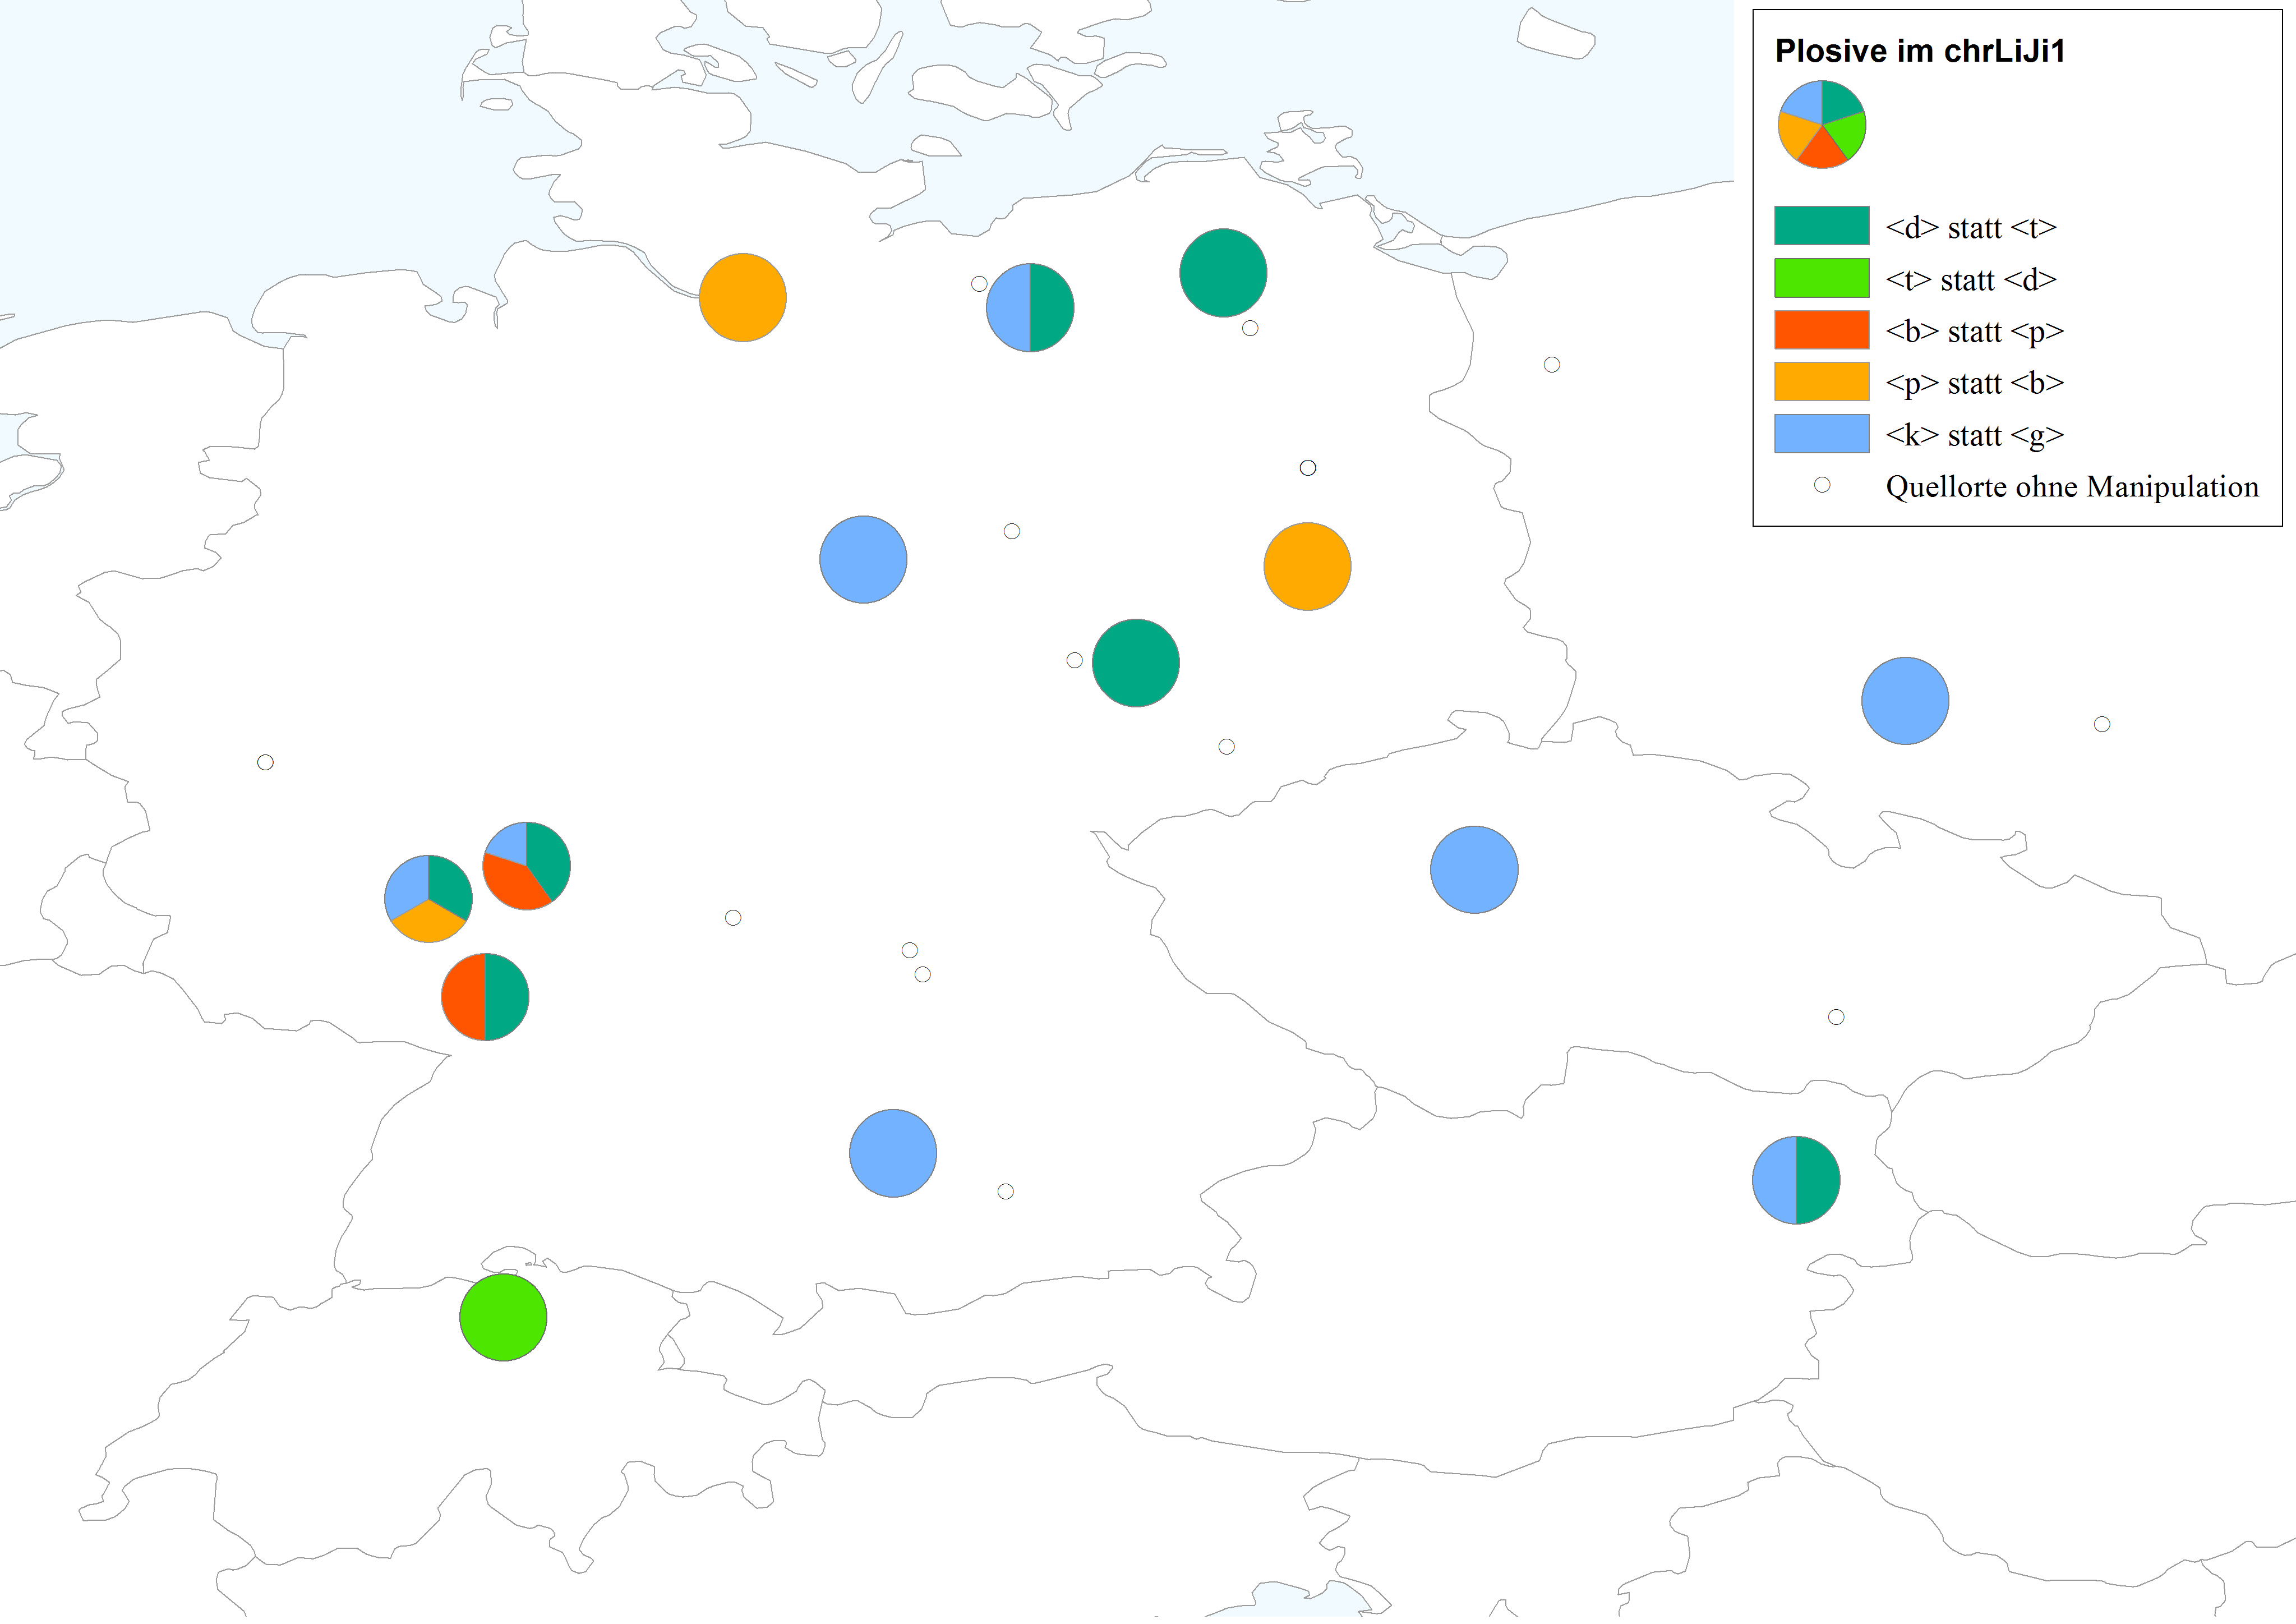
\includegraphics[scale=0.5]{figures/karte_plosive.png}
		\caption{\label{karteplosive} Orthographische Auffälligkeiten der \isi{Plosive} im \hai{chrLiJi1}}
		\end{figure}
\FloatBarrier


Die Karte in Abb. \ref{lijiphon} fasst die Summe zusammen, wie viele phonologische Phänomene (von 24 analysierten Phänomenen)\footnote{Um eine Vergleichbarkeit mit der Situation in den deutschen Dialekten zu gewährleisten (s.\,u.), wurden lediglich Phänomene aufgenommen, zu denen vergleichbare Informationen aus den Dialekten gegeben waren. Diese 24 Phänomene sind: die westjiddische Monophthongierung und der \isi{Zusammenfall} von \hai{V24} und \hai{V44}, die westjiddische Diphthongierung von \hai{V42}, \hai{V22}, \hai{V34} (< mhd. \textit{iu}), die \isi{a-Verdumpfung}, Wechsel von /o/ > /u/ und /u/ > /o/, die \isi{Palatalisierung} von /u/ > /y/, die vier Möglichkeiten der \isi{Entrundung} von /y/ und /oe/, die \isi{Koronalisierung} im An- und \isi{Auslaut}, die Lenisierungen von /ts/ > /s/, /z/ und von /t/ > /d/ und /p/ > /b/, sowie die Fortisierungen von /b/ > /p/ und /g/ > /k/, der Erhalt von westgerm. -\textit{pp}- und die Spirantisierung von /b/ > /v/.} eine Quelle verwendet. Für Orte, an denen mehr als eine Quelle vorliegt, wurde der Mittelwert aller Quellen berechnet und ist als solcher in die Kartierung eingegangen. Man sieht so, dass besonders wenige Markierungen im nördlichen und östlichen Teil des Untersuchungsgebiets auftreten. Im Zentrum, Süden und äußeren Westen hingegen findet sich eine größere Vielfalt an phonologischer Markierung. Besonders die Frankfurter Quellen und die eine belegte Münchner Quelle betreiben einen besonders hohen Aufwand bei der phonologischen Manipulation. Der generelle Durchschnitt (Mittelwert) der hier kartierten 24 Phänomene beträgt, bei einer relativ hohen Standardabweichung von 3,38, im \hai{chrLiJi1} 6,45 Phänomene pro Ort. \\

\begin{figure}[h!]
		\centering
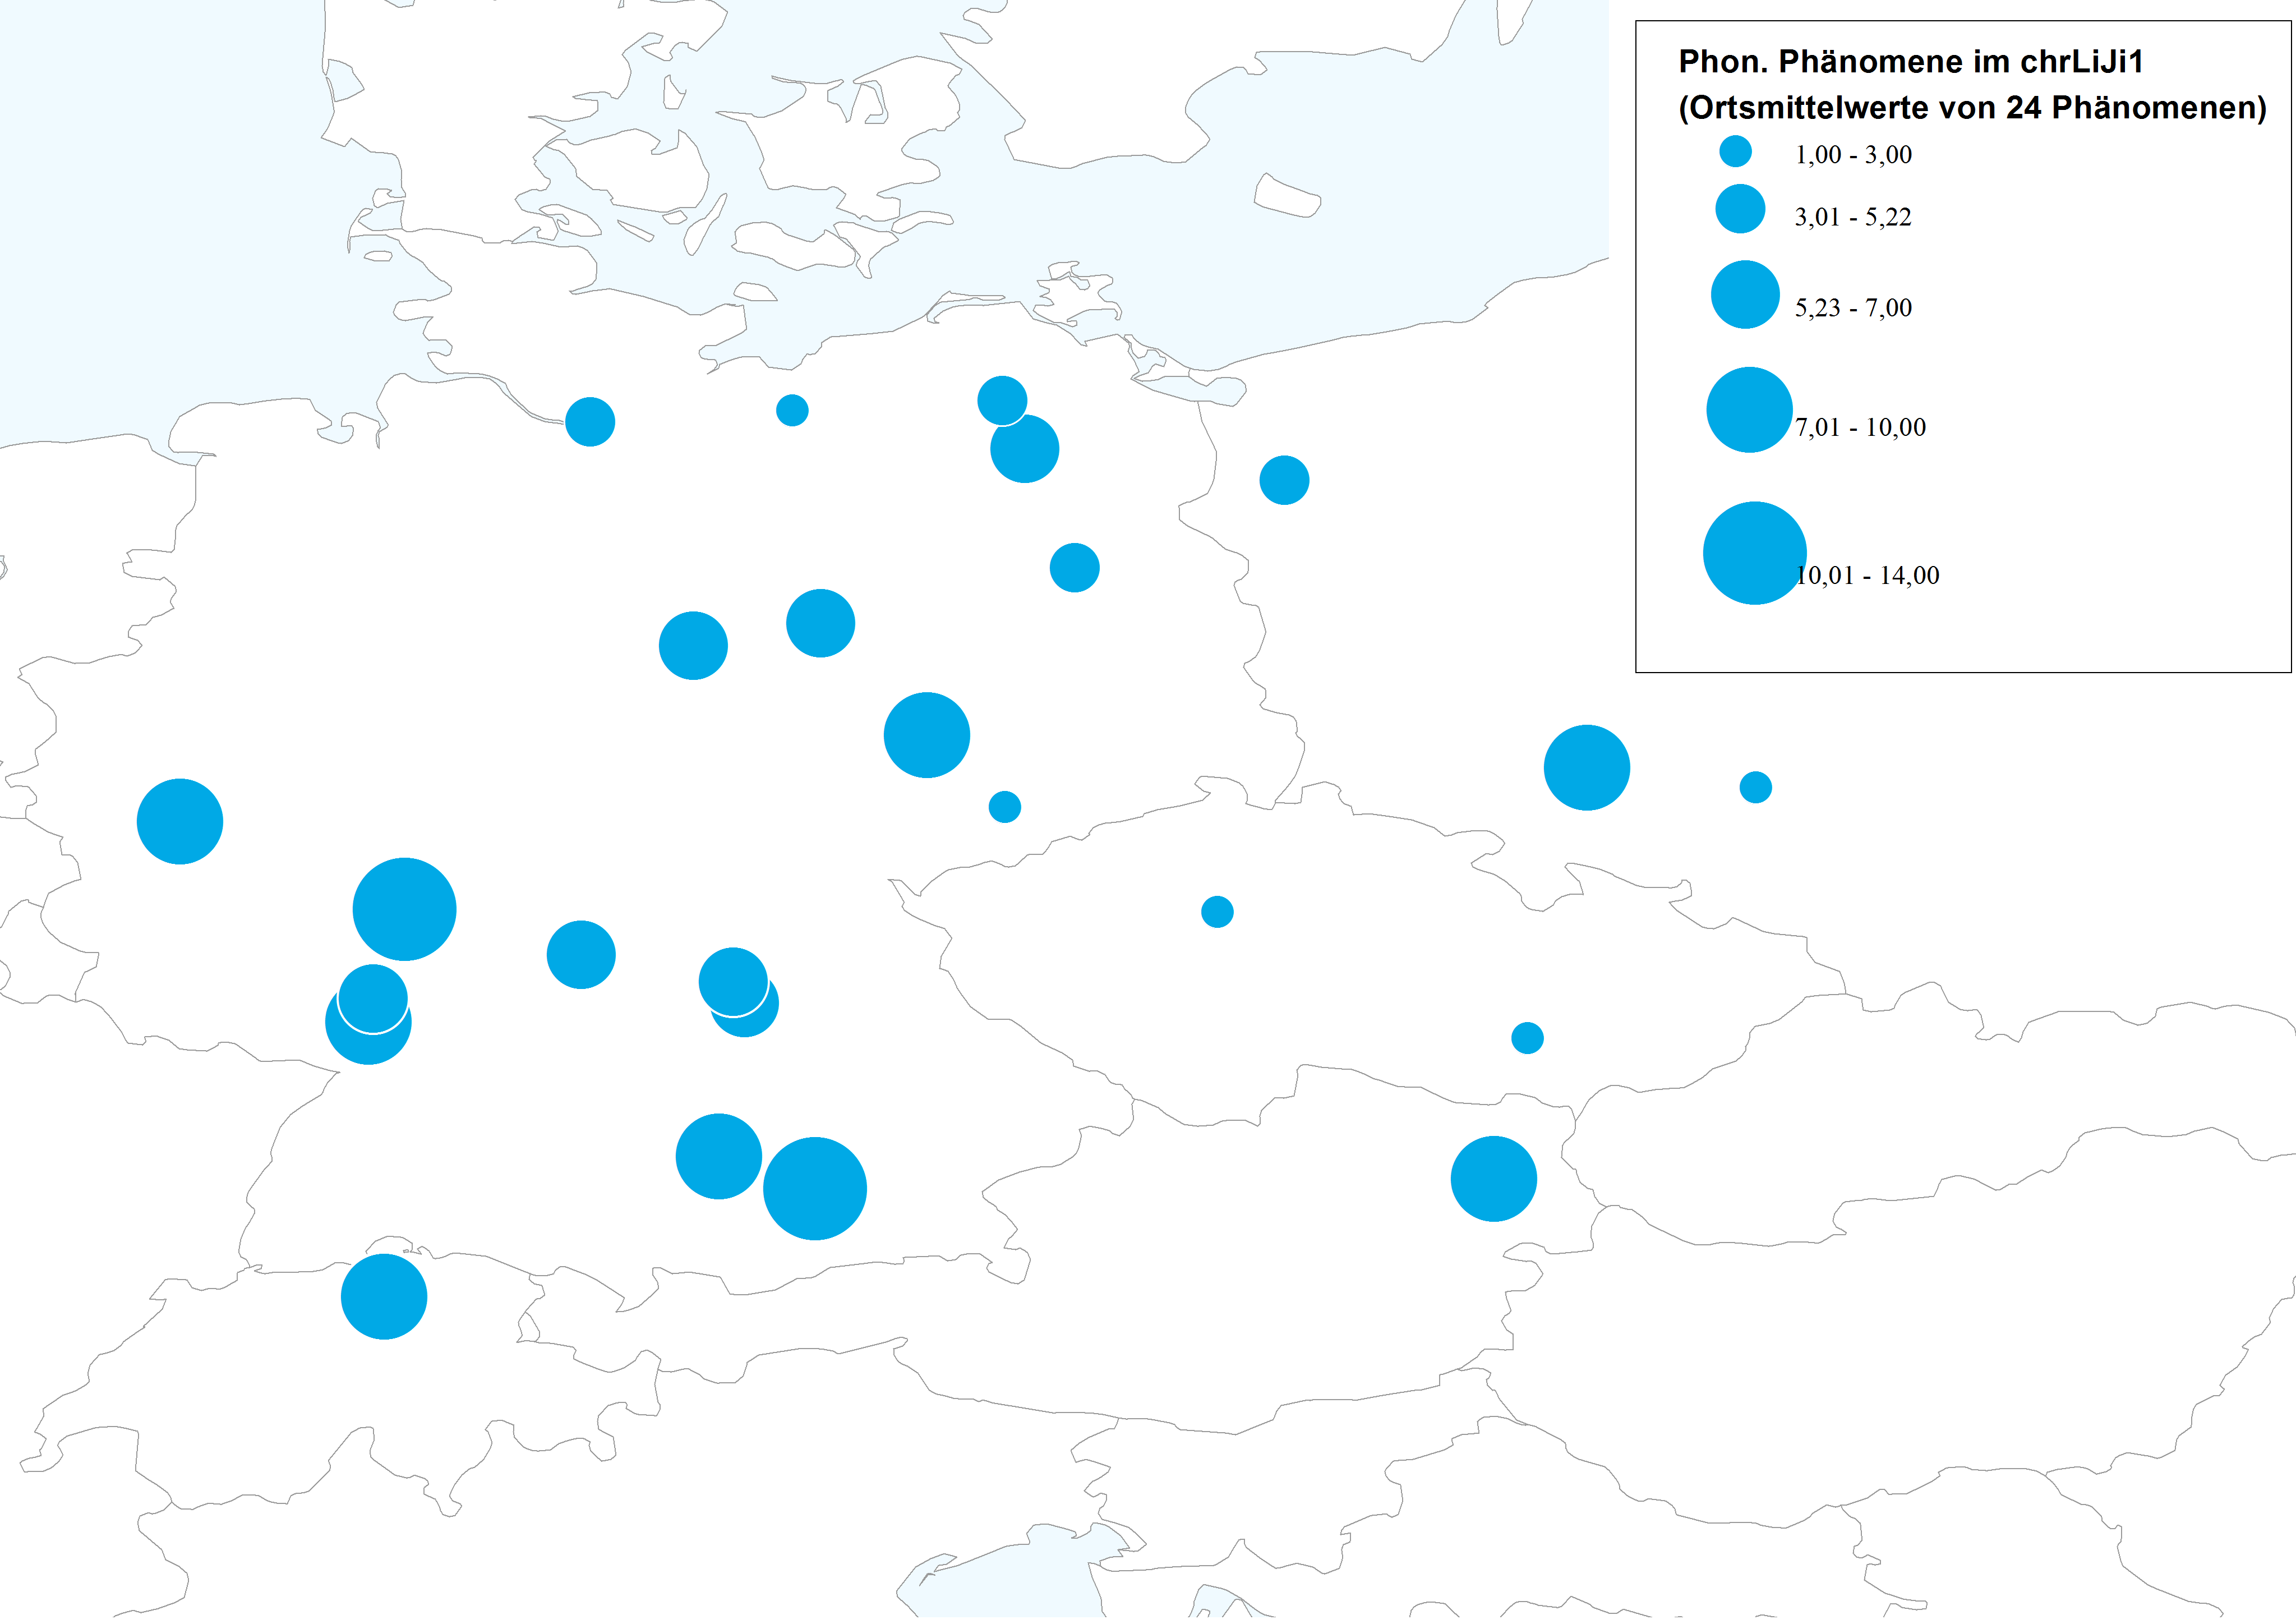
\includegraphics[scale=0.5]{figures/phon_chrliji1.png}
		\caption{\label{lijiphon} Summe phonologischer Phänomene im \hai{chrLiJi1} (Ortsmittelwerte)}
\end{figure}
\FloatBarrier


Für Karte \ref{kartelijiIDW} wurden die Daten aus Karte \ref{lijiphon} mittels inverser Distanzwichtung (Inverse Distance Weighting, kurz \hai{IDW}) interpoliert.\footnote{Die \hai{IDW} wurde hier nach der im Spatial Analyst Modul des Kartierungsprogramms \hai{ArcGIS 10.1} (ESRI Inc.) und/oder des entsprechenden Tools des Karierungsprogramms \hai{QGIS} (Version 2.4 \textit{Chugiak}) festgelegten Formel berechnet und wie alle Karten dieser Arbeit mit eben diesem Programm erstellt. Dabei werden zunächst, wie bei jeder Form von Interpolation, die gegebenen Datenwerte  \hai{Z\textsubscript{1}}, ...,  \hai{Z\textsubscript{n}} die mit unterschiedlichen Orten verknüpft sind \hai{P\textsubscript{1}}, ..., \hai{P\textsubscript{n}} miteinander in Beziehung gestellt. Der interpolierte Wert ist ein gewichteter Durchschnitt aller Datenwerte. Die \textit{Abweichungen} (\textit{Schwere}, \textit{weights}) der einzelnen Datenpunkte zu diesem Durchschnitt ist \hai{w}. Um den tatsächlichen Mittelwert zu ermitteln muss durch die Summe aller \textit{Abweichungen} geteilt werden: 
\begin{math} 
Z = \frac{[w\textsubscript{1} \cdot Z\textsubscript{1} + ... + w\textsubscript{n} \cdot Z\textsubscript{n}]}  {[w\textsubscript{1} + ... + w\textsubscript{n}]}
\end{math}
. Bei einer \hai{IDW} wird der Grad der \textit{Abweichung} durch den Wert \hai{p} beeinflusst. Dieser gewährleistet dass die Abweichungen zwischen  Datenpunkt (\hai{P}) und Interpolationspunkt (\hai{P}\textsubscript{i}) proportional verlaufen: 
\begin{math} w\textsubscript{i} = \frac{1} {Abstand(P, P\textsubscript{i})^p} \end{math} . Für \hai{p} wurde der Wert \hai{p}=2 gesetzt. Der Zahlenwert selbst spielt nur eine geringe Rolle; zentral ist, dass alle \hai{P}-Werte durch einen gemeinsamen \hai{p}-Wert normalisiert sind (vgl. \cite[132–160]{BurroughMcDonnell1998}).} Dies ermöglicht eine bessere räumliche Darstellung. Damit erkennt man deutlich, dass das \hai{chrLiJi1} besonders vielfältig phonologische Manipulationen einsetzt und sich ein gewisser Grad der Abnahme gegen Nordosten ergibt.\\ 
  
 \begin{figure}[h!]
		\centering
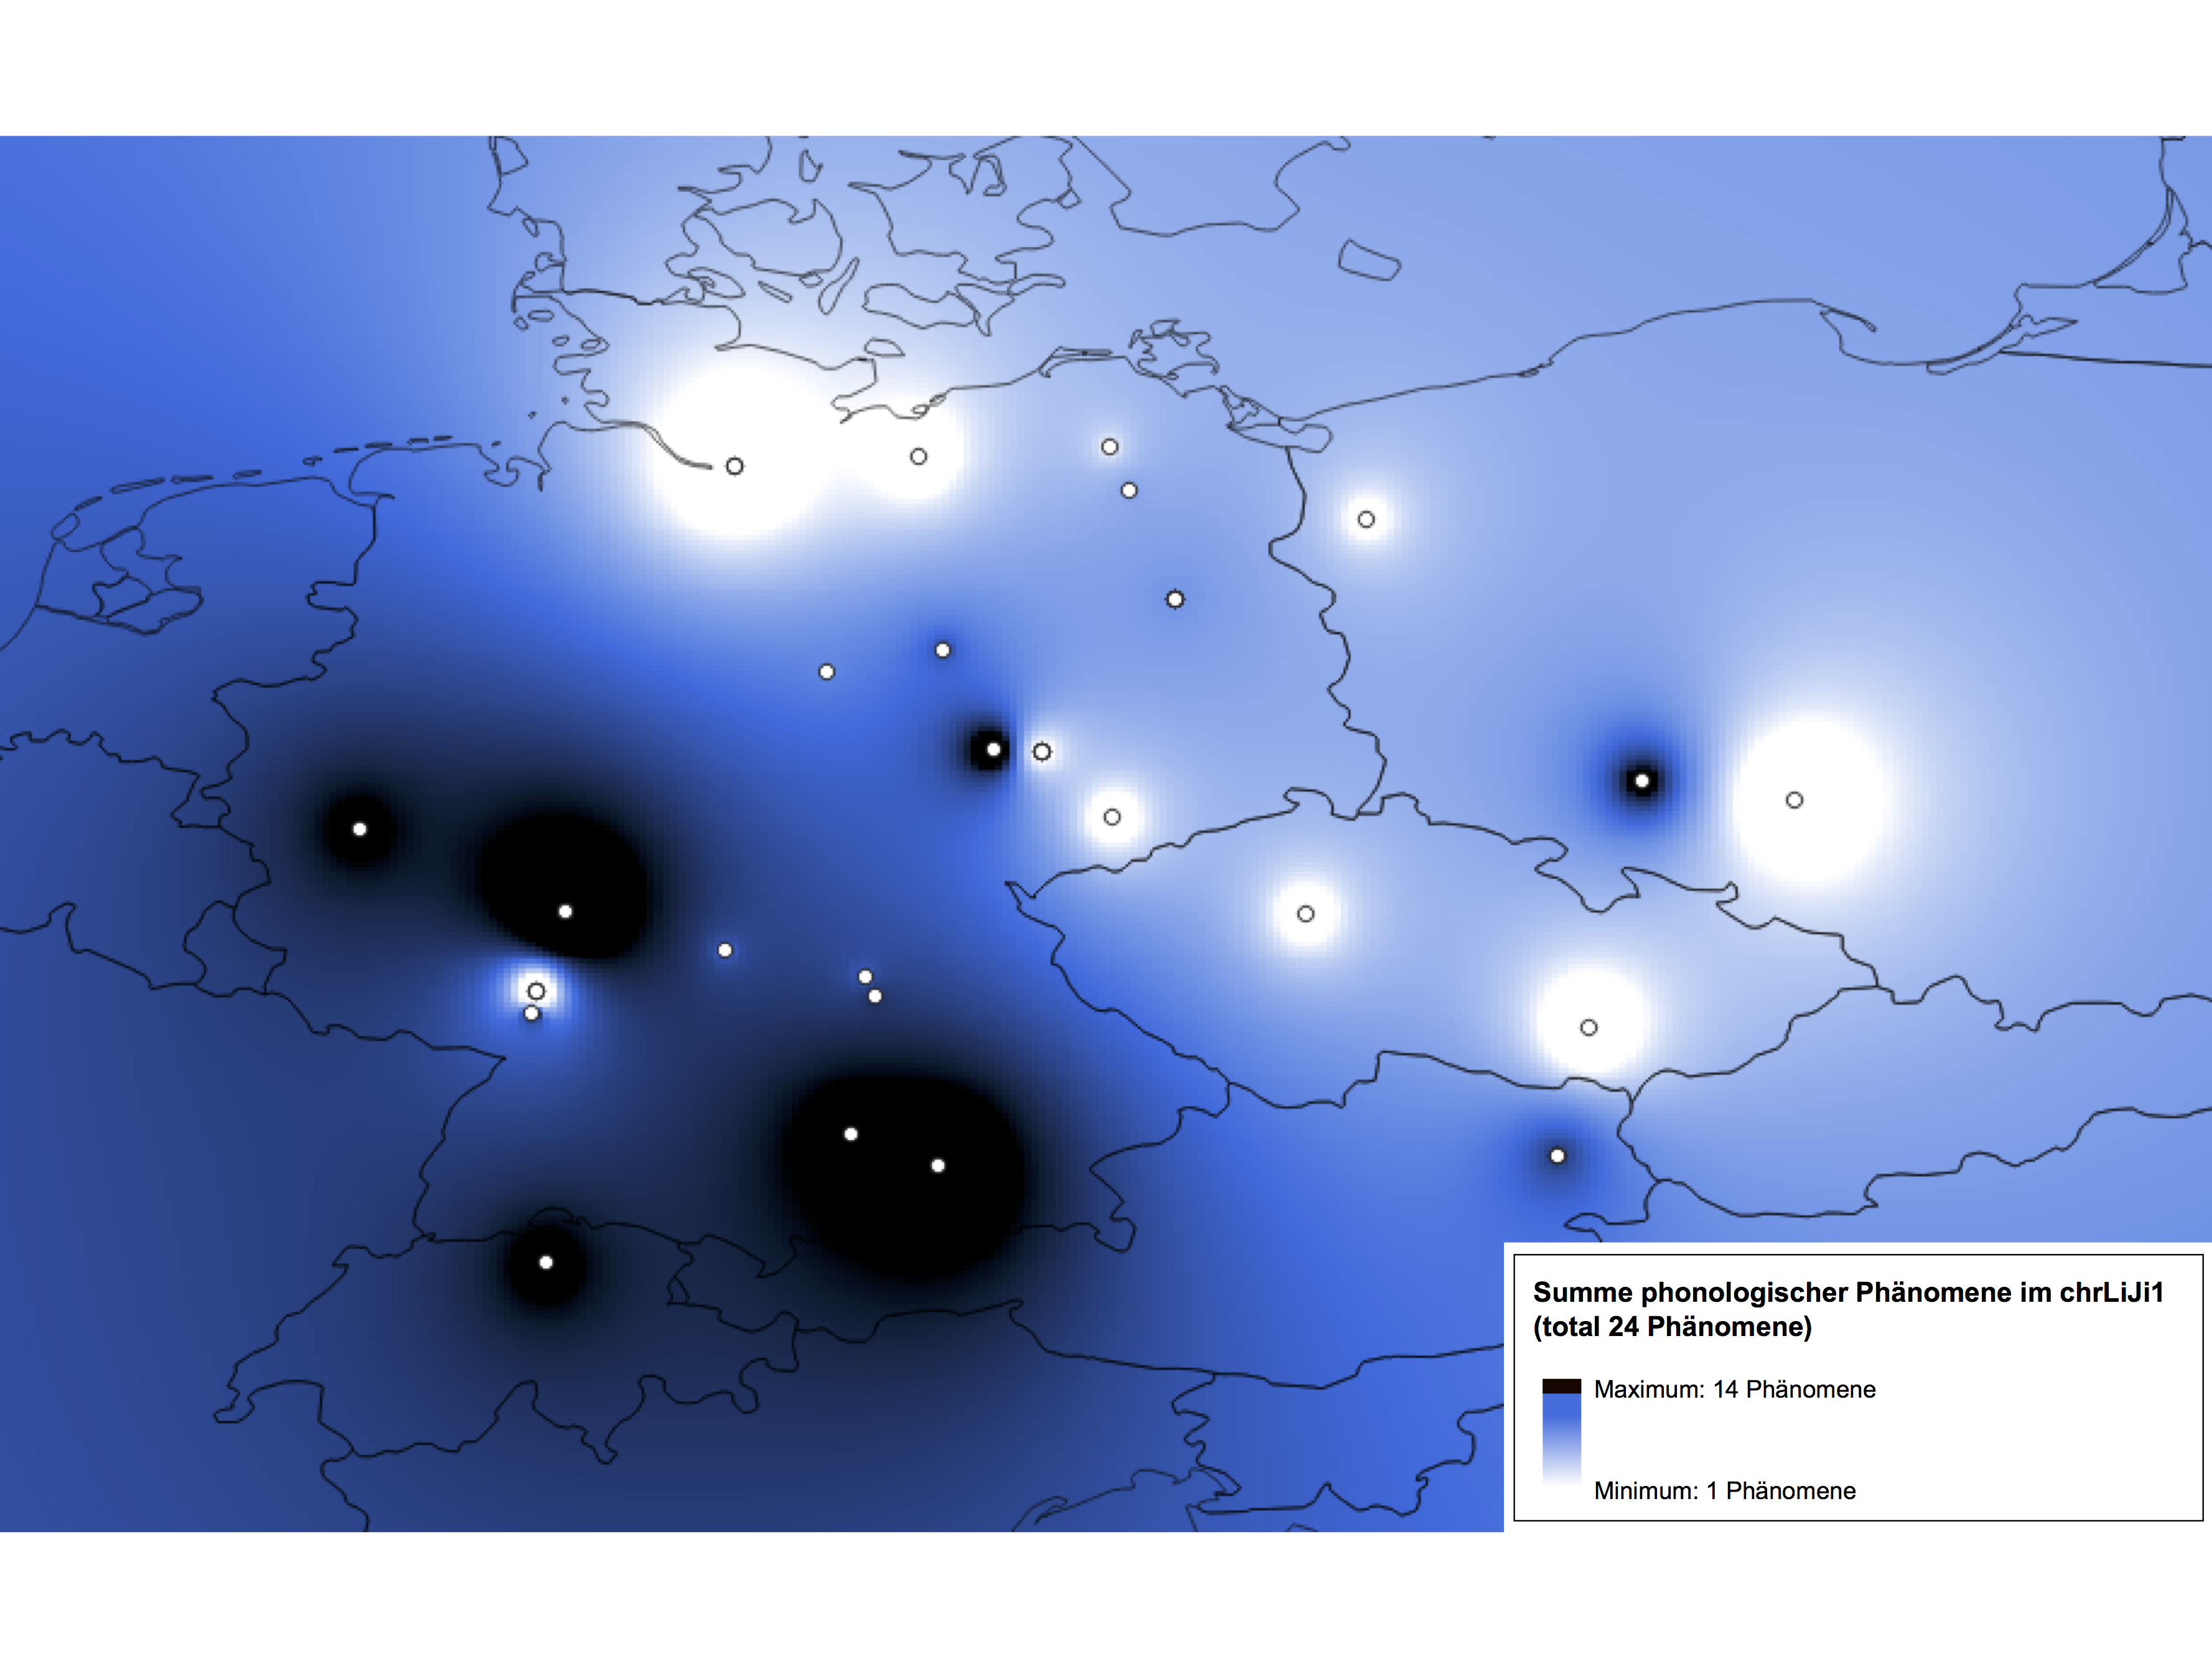
\includegraphics[scale=0.75]{figures/phon_IDW_legende.png}
		\caption{\label{kartelijiIDWQGIS} Summe phonologischer Phänomene im \hai{chrLiJi1} (\hai{IDW} berechnet mit \hai{QGIS})}
		\end{figure}
		
		
\begin{figure}[h!]
		\centering
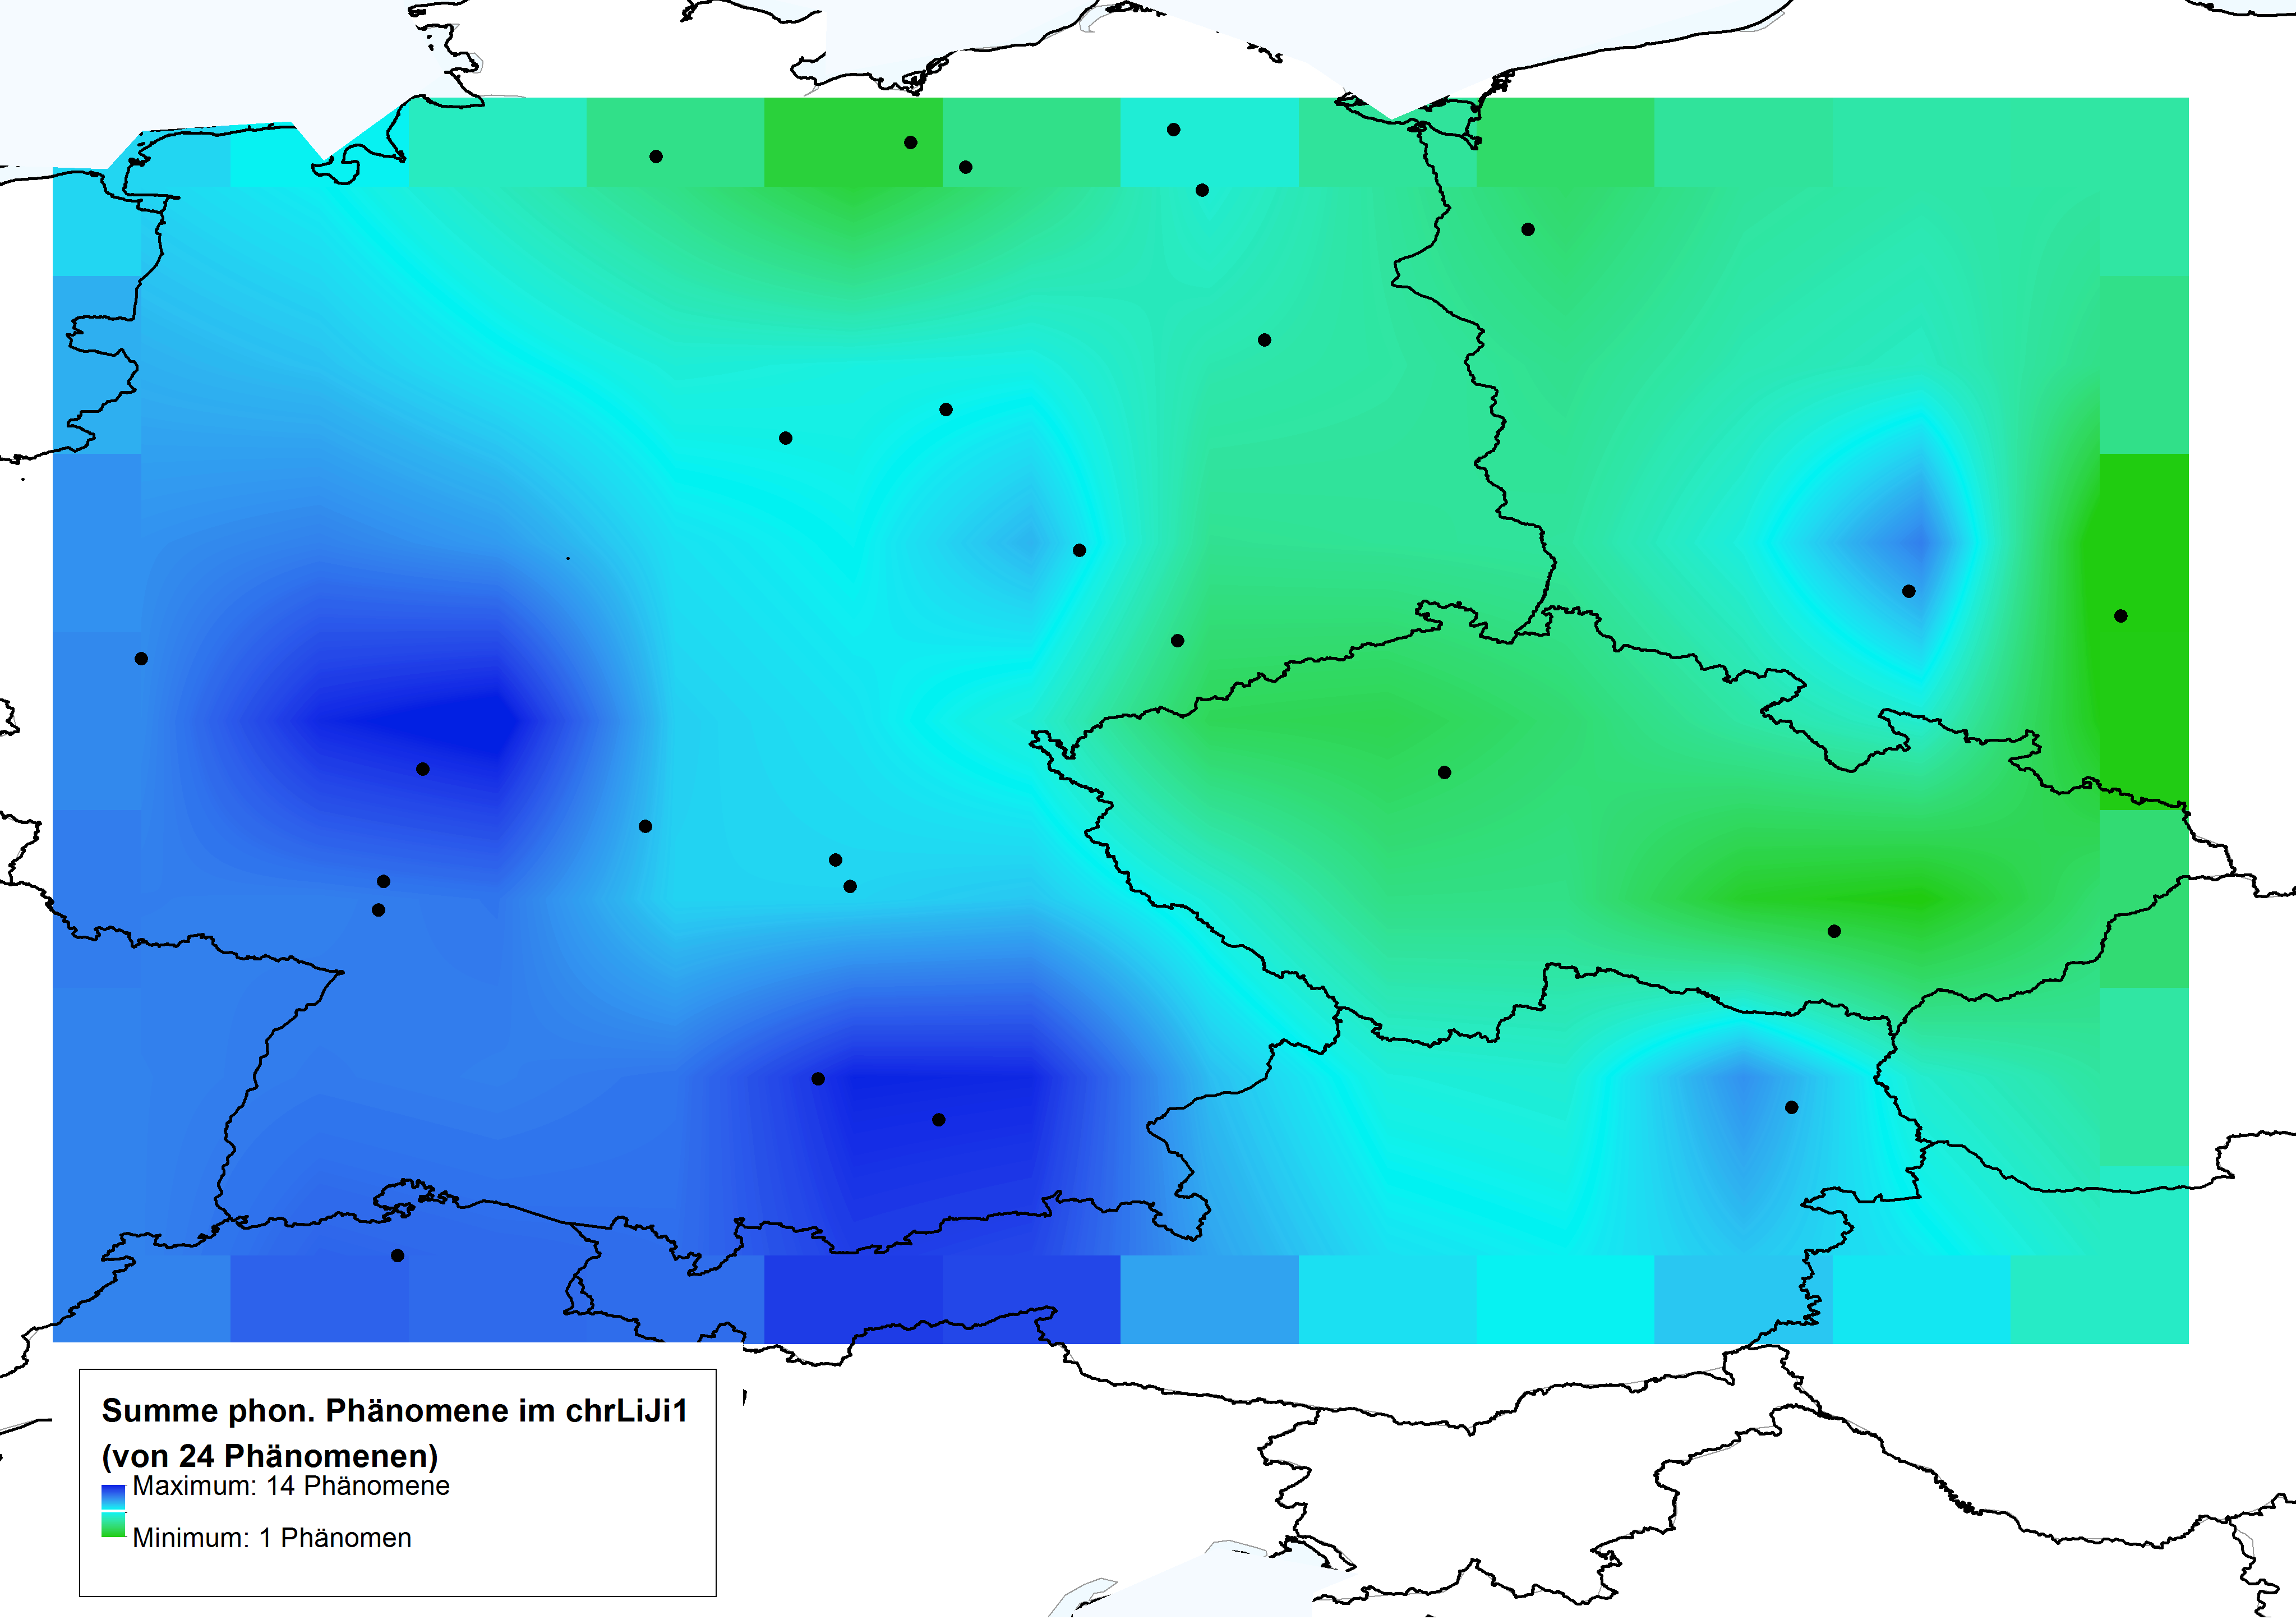
\includegraphics[scale=0.4]{figures/phon_liji_nurIDW_PUNKT.png}
		\caption{\label{kartelijiIDW} Darstellung der Abstufungen der Summe phonologischer Phänomene im \hai{chrLiJi1} (\hai{IDW})}
		\end{figure}
\FloatBarrier


Da ein gewisser Einfluss der örtlichen Dialekte auf das \hai{chrLiJi1} denkbar ist, wurden zu den einzelnen Orten des \hai{chrLiJi1} die entsprechenden Situationen in den deutschen Dialekten aufgenommen und sofern diese deckungsgleich mit den phonologischen Phänomenen des \hai{chrLiJi1}, sind in der Karte \ref{allphondt} kartiert und in Karte \ref{IDWphondt} mittels \hai{IDW} interpoliert.\footnote{Die Daten zu den deutschen Dialekten ergeben sich aus den in den Einzelanalysen herangezogenen Quellen, sprich vorwiegend den Daten des \hai{WA} u. des \hai{KDSA}.} Der Mittelwert aller deutschen Dialekte zu den Phänomenen ist mit  6,31 Phänomenen pro Ort sehr ähnlich wie im \hai{chrLiJi1}; die Standardabweichung beträgt hier 3,6. Es zeigt sich hier besonders in Mittel- und Süddeutschland (und Österreich), dass aus den deutschen Dialekten potentiell mehr Phänomene bekannt hätten sein müssen, als sie im \hai{chrLiJi1} verwendet wurden. Andere Quellen wie etwa im Frankfurter, Mannheimer, Augsburger und Breslauer Raum zeigen eine ähnliche Anzahl an Phänomenen im \hai{chrLiJi1} wie auch in den deutschen Dialekten. Die Karte \ref{allphondt} zeigt uns darüber hinaus, dass das \hai{LiJi1} eine Vielzahl phonologischer Phänomene mit den deutschen Dialekte, insbesondere den rheinfränkischen und obersächsischen, teilt. Der Vergleich der Karten \ref{IDWphondt} und \ref{kartelijiIDW} zeigt, dass besonders die südöstlichen Quellen (München, Augsburg, Erlangen, Nürnberg) eine Vielzahl phonologischer Manipulationen aufweisen, die am Ortsdialekt selbst nicht vorhanden sind. \\




 \begin{figure}[h!]
		\centering
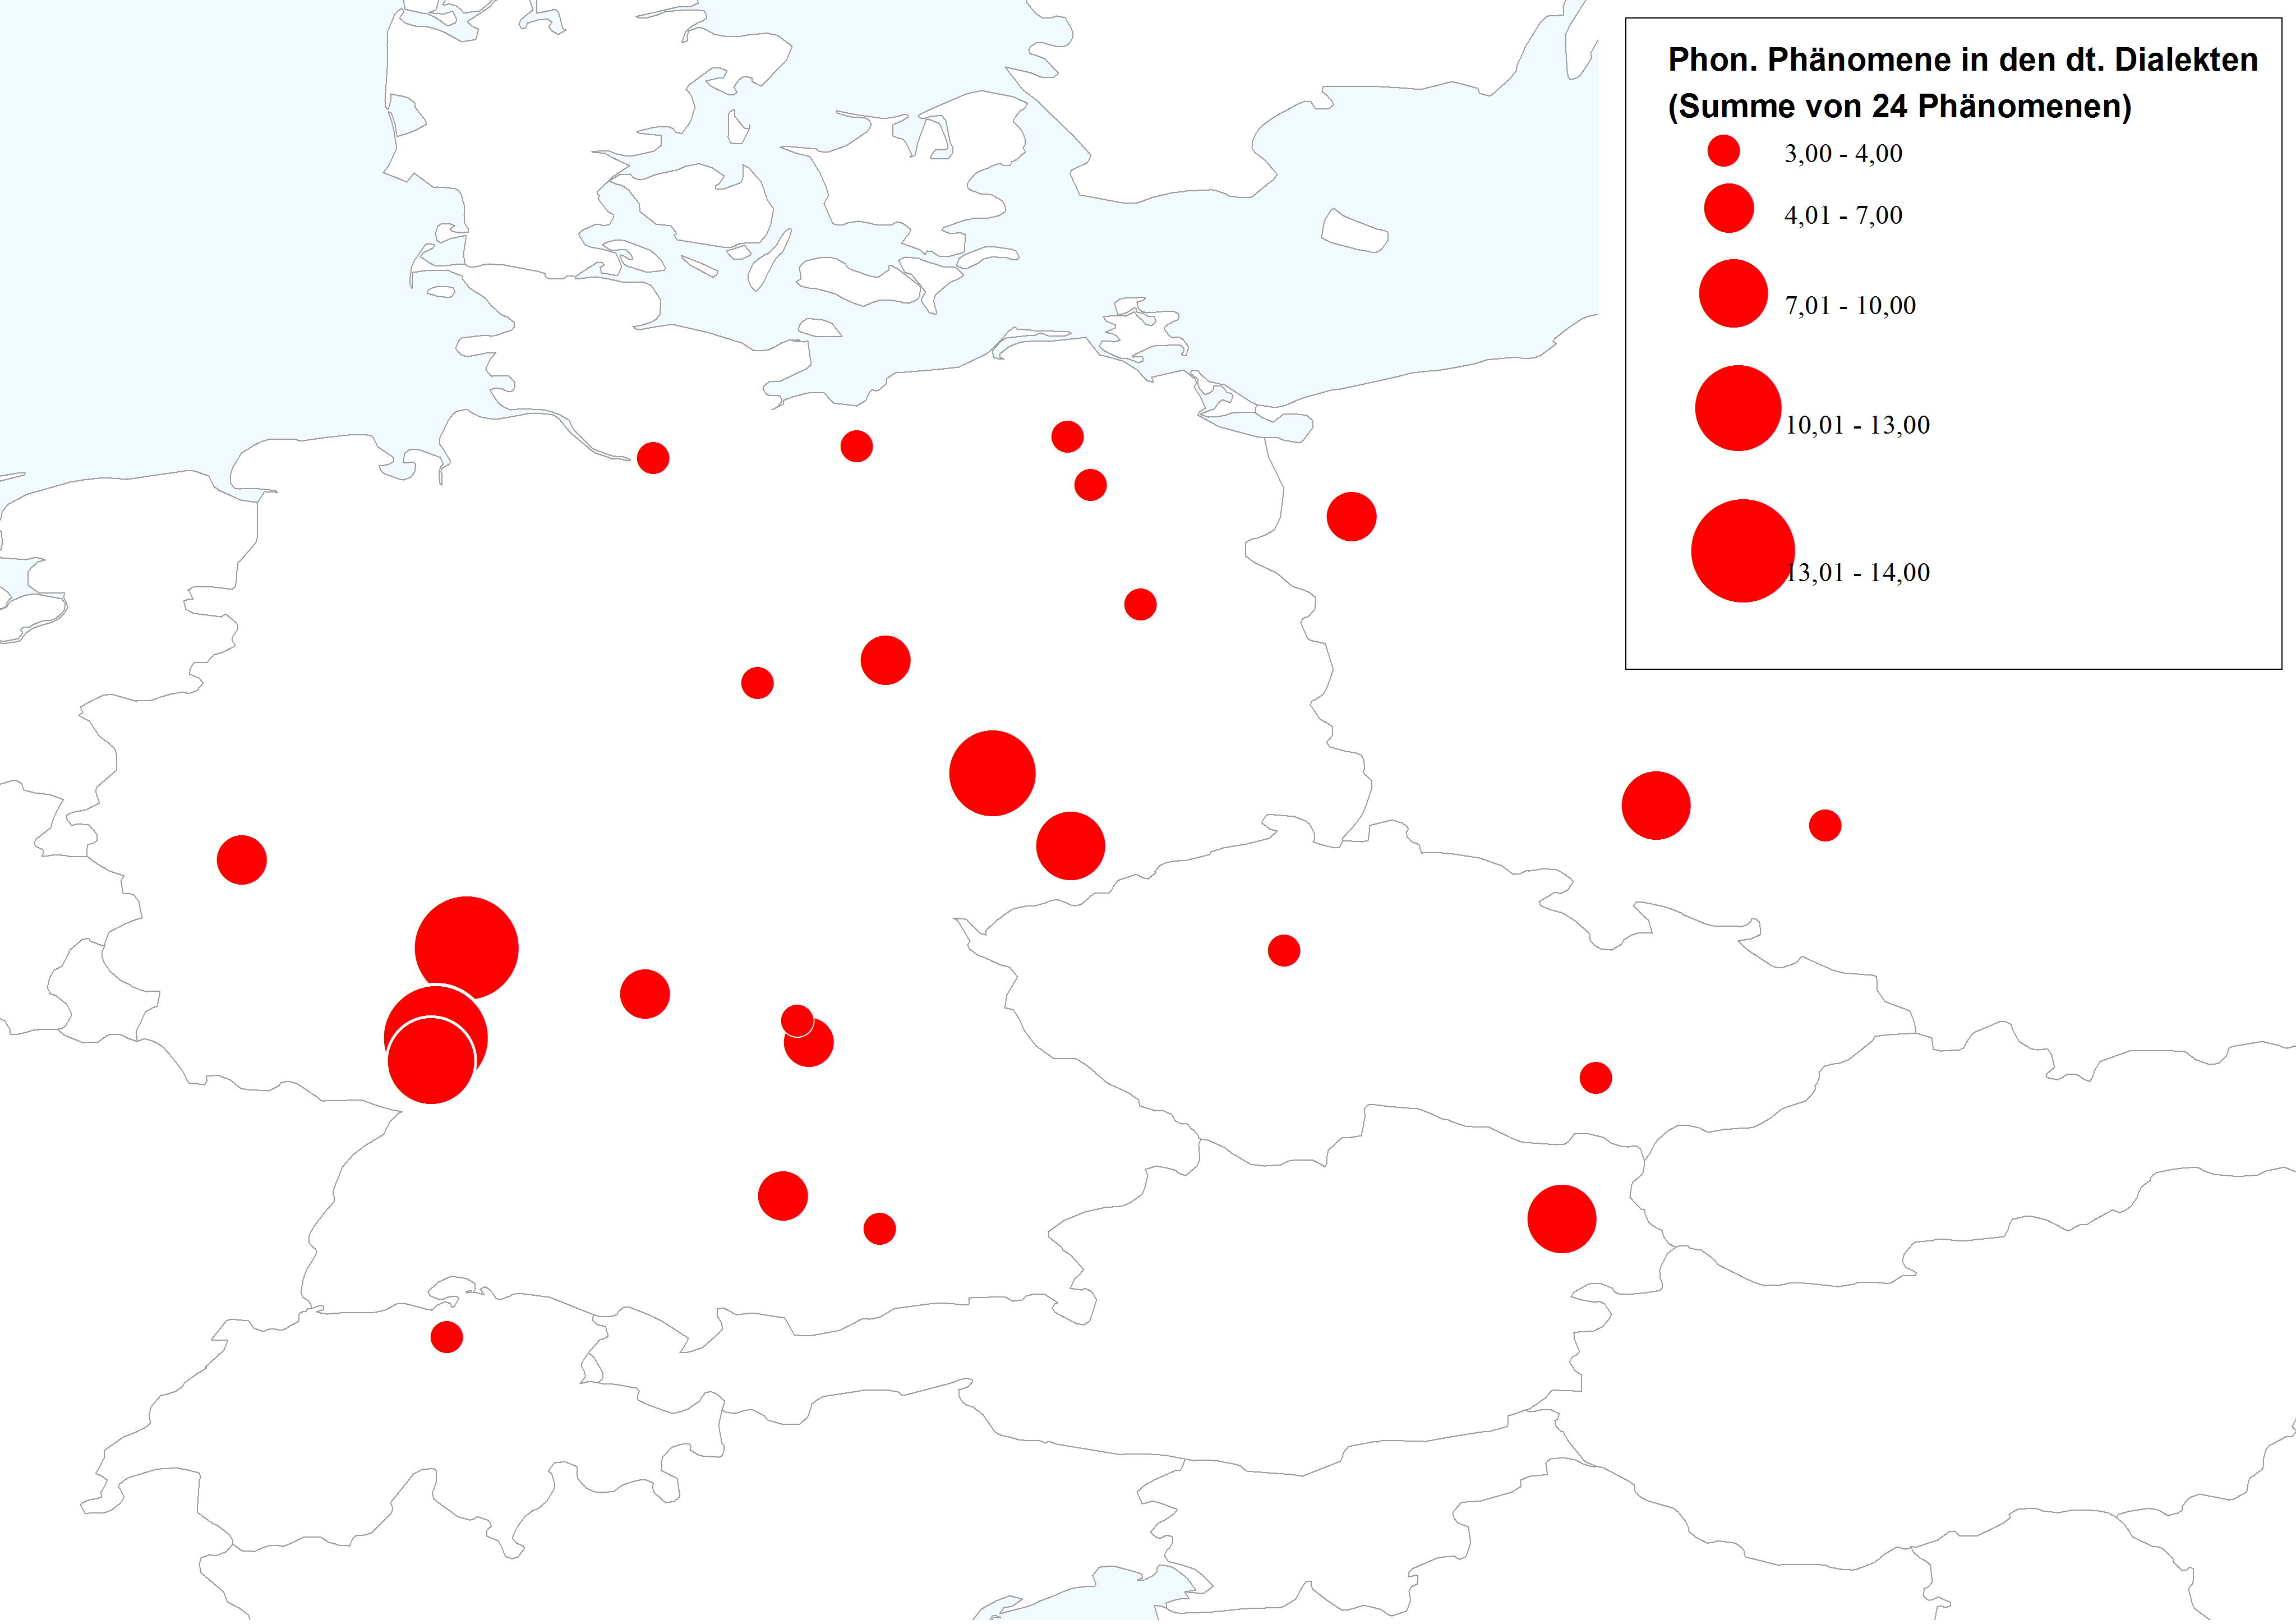
\includegraphics[scale=0.4]{figures/phon_dt_dialekte.png}
		\caption{\label{allphondt} Summe phonologischer Phänomene des \hai{chrLiJi1} in den entsprechenden dt. Dialekten}
		\end{figure}
		
		
\begin{figure}[h!]
		\centering
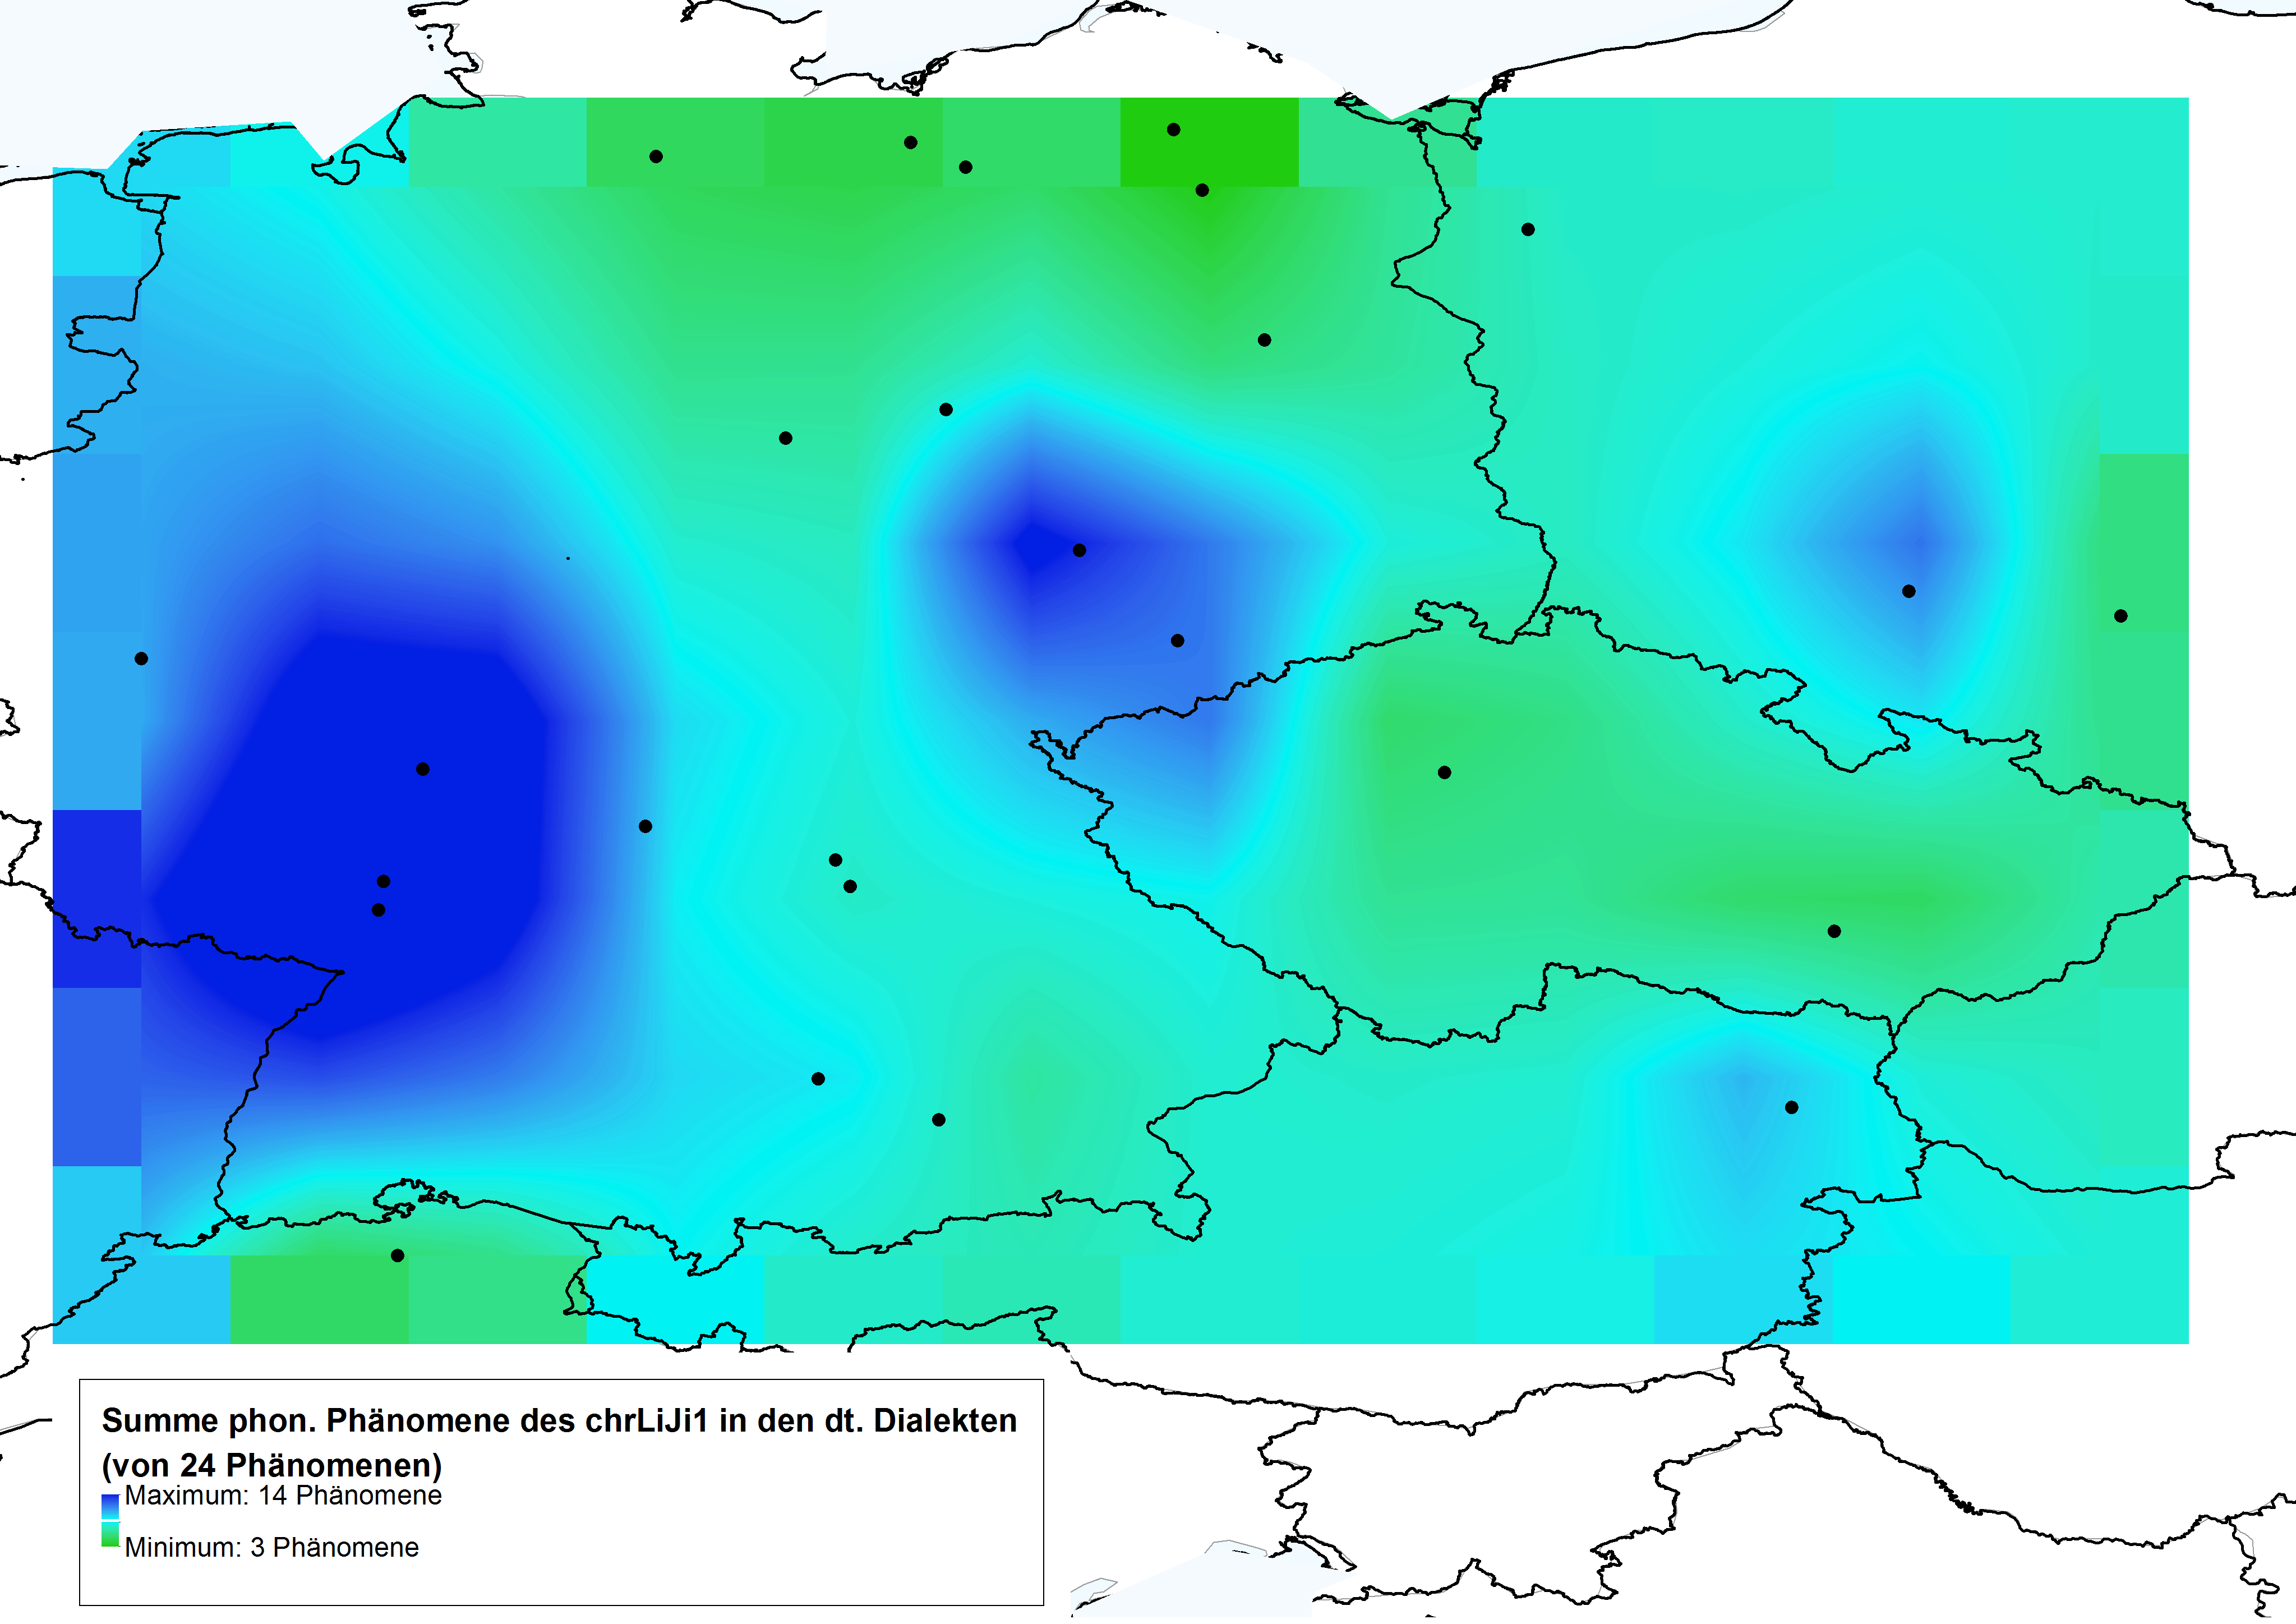
\includegraphics[scale=0.4]{figures/phon_dt_nurIDW_PUNKT.png}
		\caption{\label{IDWphondt} Summe phonologischer Phänomene des \hai{chrLiJi1} in den entsprechenden dt. Dialekten (\hai{IDW})}
		\end{figure}
\FloatBarrier
		
	Doch diese Daten alleine zeigen nur die reine Quantität phonologischer Phänomene und noch nicht, welche Phänomene, die an einem Ort im \hai{chrLiJi1} vorliegen, auch im entsprechenden deutschen Dialekt belegt sind. Die genaue Schnittmenge zwischen phonologischen Phänomenen, die im \hai{chrLiJi1} an einem Ortspunkt gewählt werden und die selbst im Ortsdialekt verbreitet sind, findet sich in den Karten \ref{allphondtliji} und \ref{IDWallphondtliji} dargestellt. Hier sticht der rheinfränkische Raum deutlich heraus. Und auch im Schlesischen, Obersächsischen und im Mittelbairischen Wiens gibt es starke Übereinstimmungen zwischen den im \hai{chrLiJi1} verwendeten phonologischen Manipulationen, die auch im deutschen Dialekt bekannt sind. Dabei muss beachtet werden, dass dies auch die Dialekträume sind, in denen generell die im \hai{chrLiJi1} verwendeten Phänomene auftreten (vgl. Karten \ref{allphondt} und \ref{IDWphondt}). Auch dürfen diese Karten nicht so gelesen werden, dass im \hai{chrLiJi1} besonders phonologische Phänomene aus den deutschen Dialekten genutzt wurden, sondern diese Daten veranschaulichen lediglich die Nähe der eingesetzten Phänomene zum Ortsdialekt. Wie in den Einzelanalysen gezeigt werden konnte, sind alle bisher behandelten Phänomene mehr oder weniger auf authentische jiddische Formen zurückzuführen. \hai{LiJi1} ist also nicht bloß eine wahllose Zusammenschau verschiedener, in den deutschen Dialekten ohnehin weit verbreiteter Phänomene, sondern ein in sich durchaus stabiles  sprachliches System, was besonders der diachrone Blick auf die einzelnen Phänomene unterstreicht (vgl. Abb. \ref{phonwjallstreu}). Die arealen Muster, die sich in den hier vorliegenden Karten erkennen lassen, sind besonders dem Umstand geschuldet, dass die (west-)jiddische Phonologie viele Eigenschaften mit den mitteldeutschen Mundarten teilt.\\


 \begin{figure}[h!]
		\centering
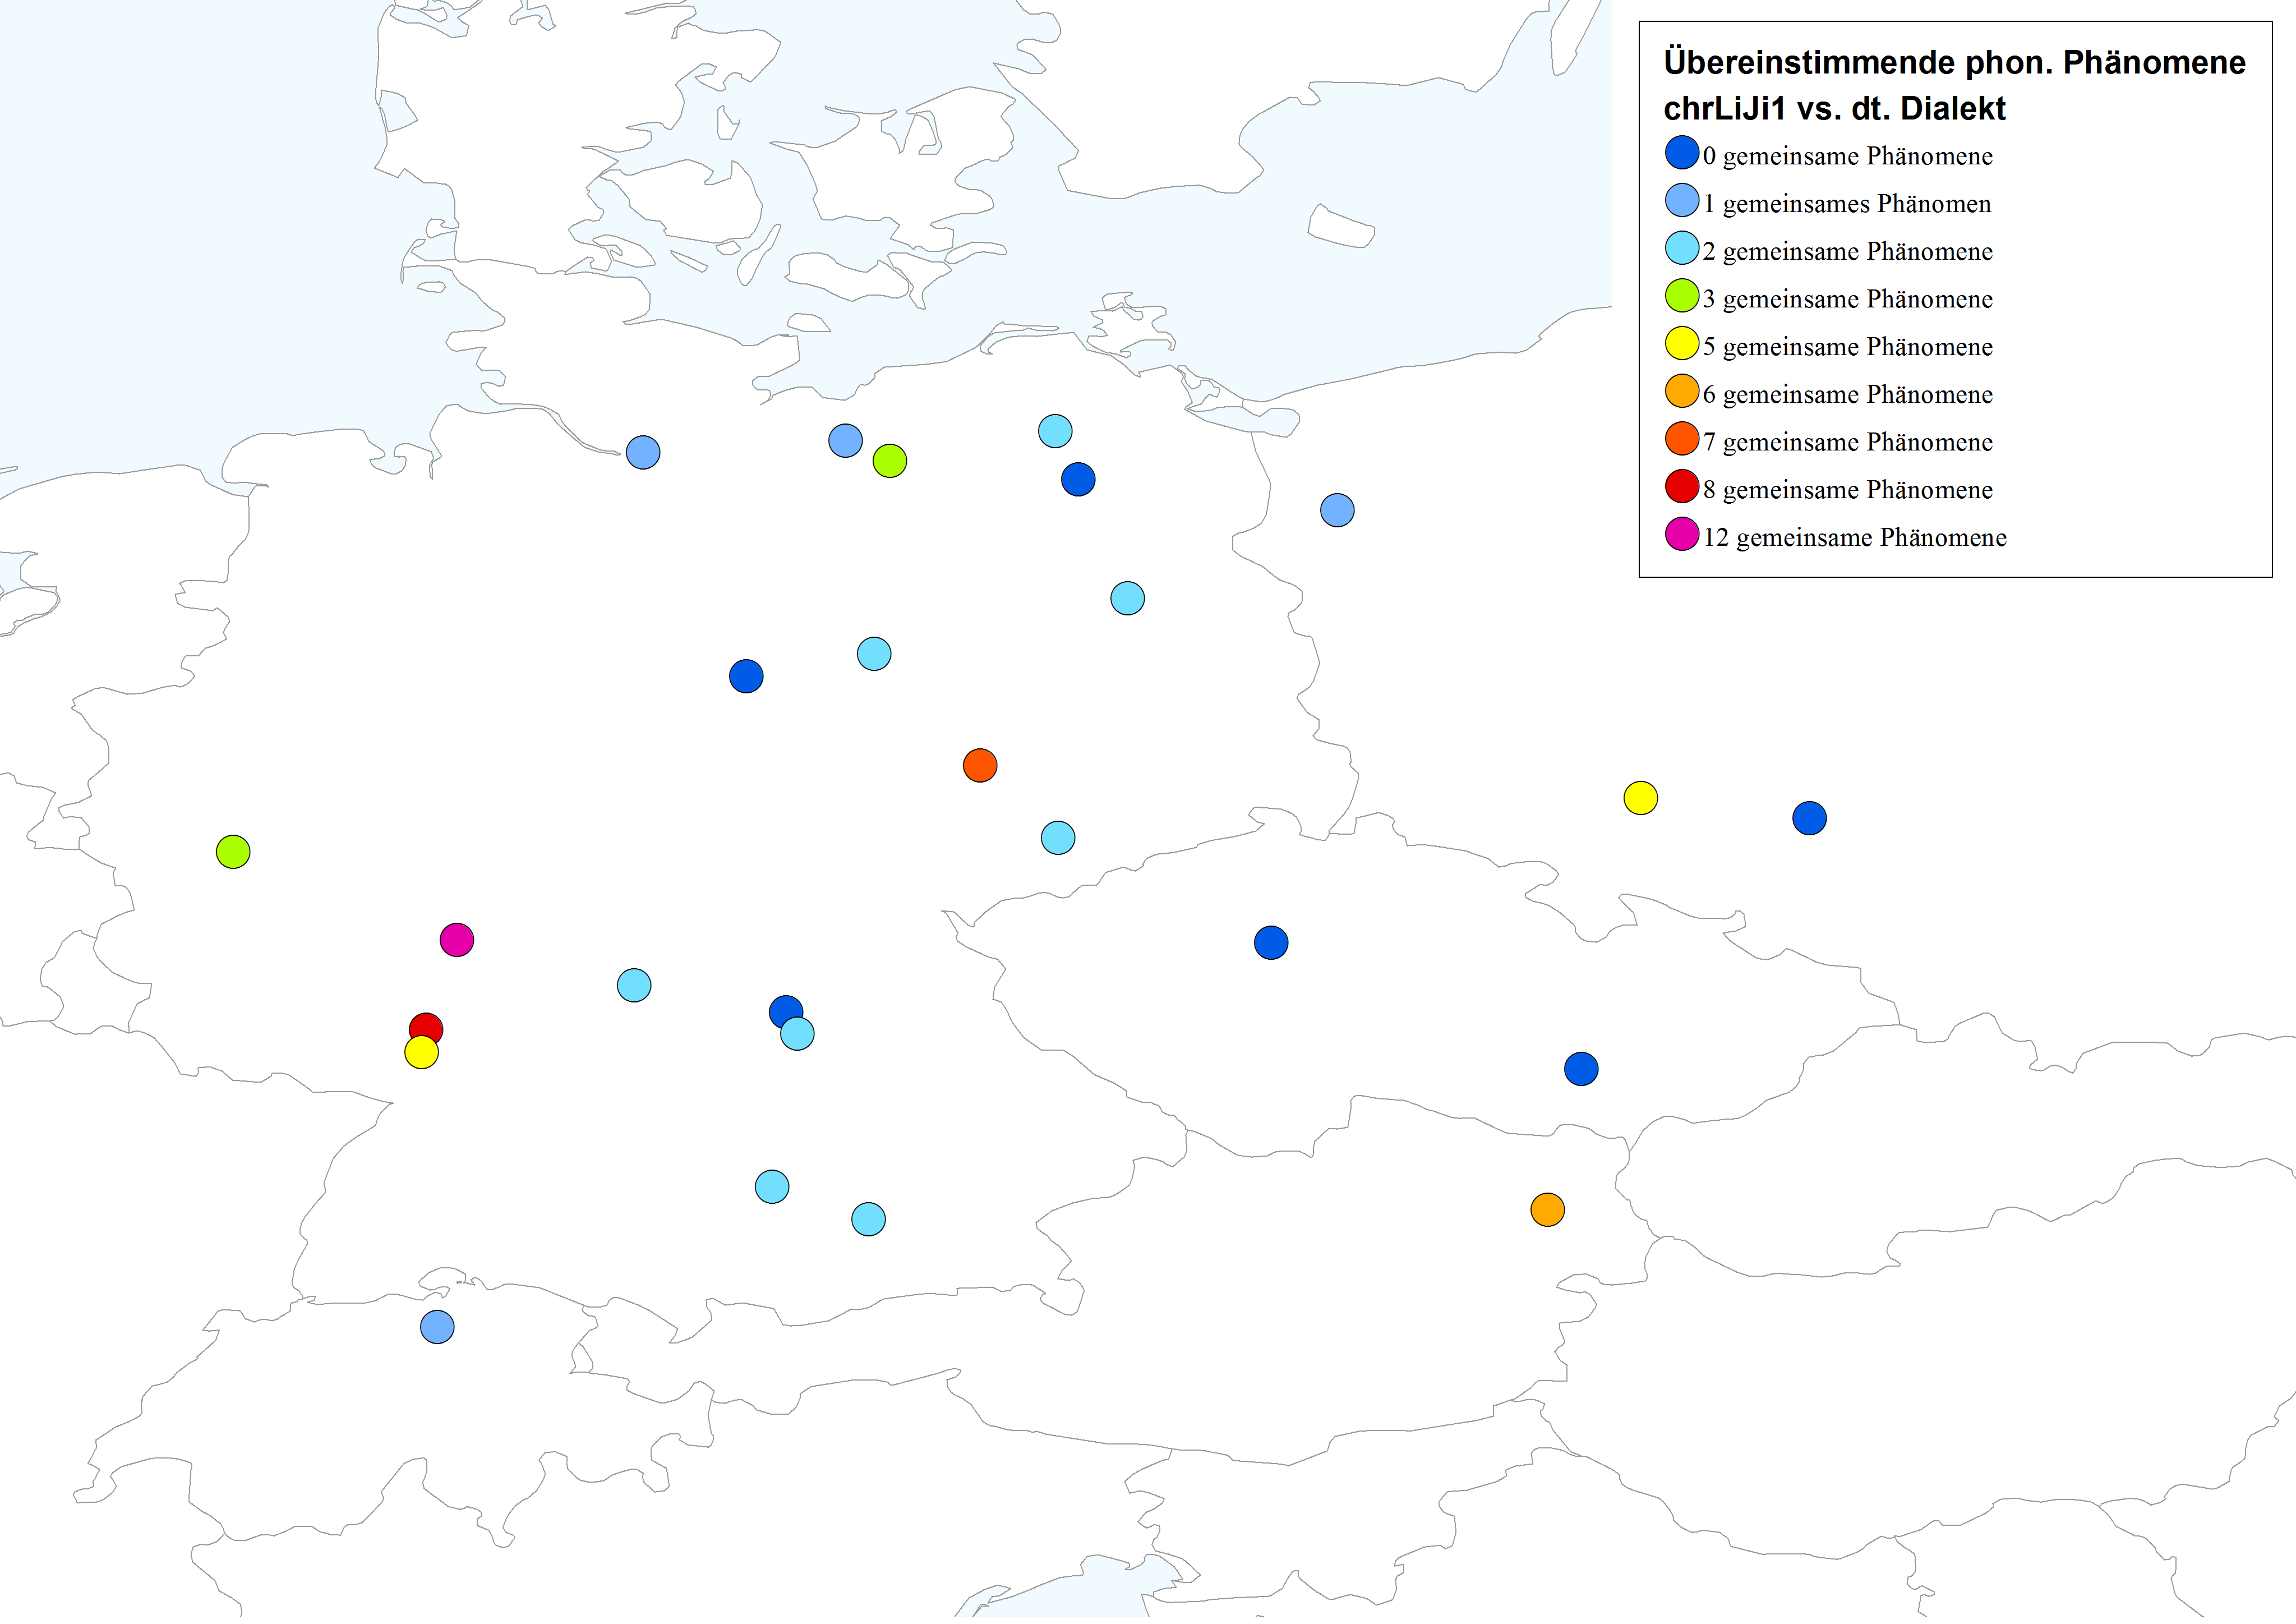
\includegraphics[scale=0.42]{figures/Uebereinstimmung_phon_liji_dt.png}
		\caption{\label{allphondtliji} Gemeinsame phonologische Phänomene des \hai{chrLiJi1} und der entsprechenden dt. Dialekte}
		\end{figure}
 
 
 
 \begin{figure}[h!]
		\centering
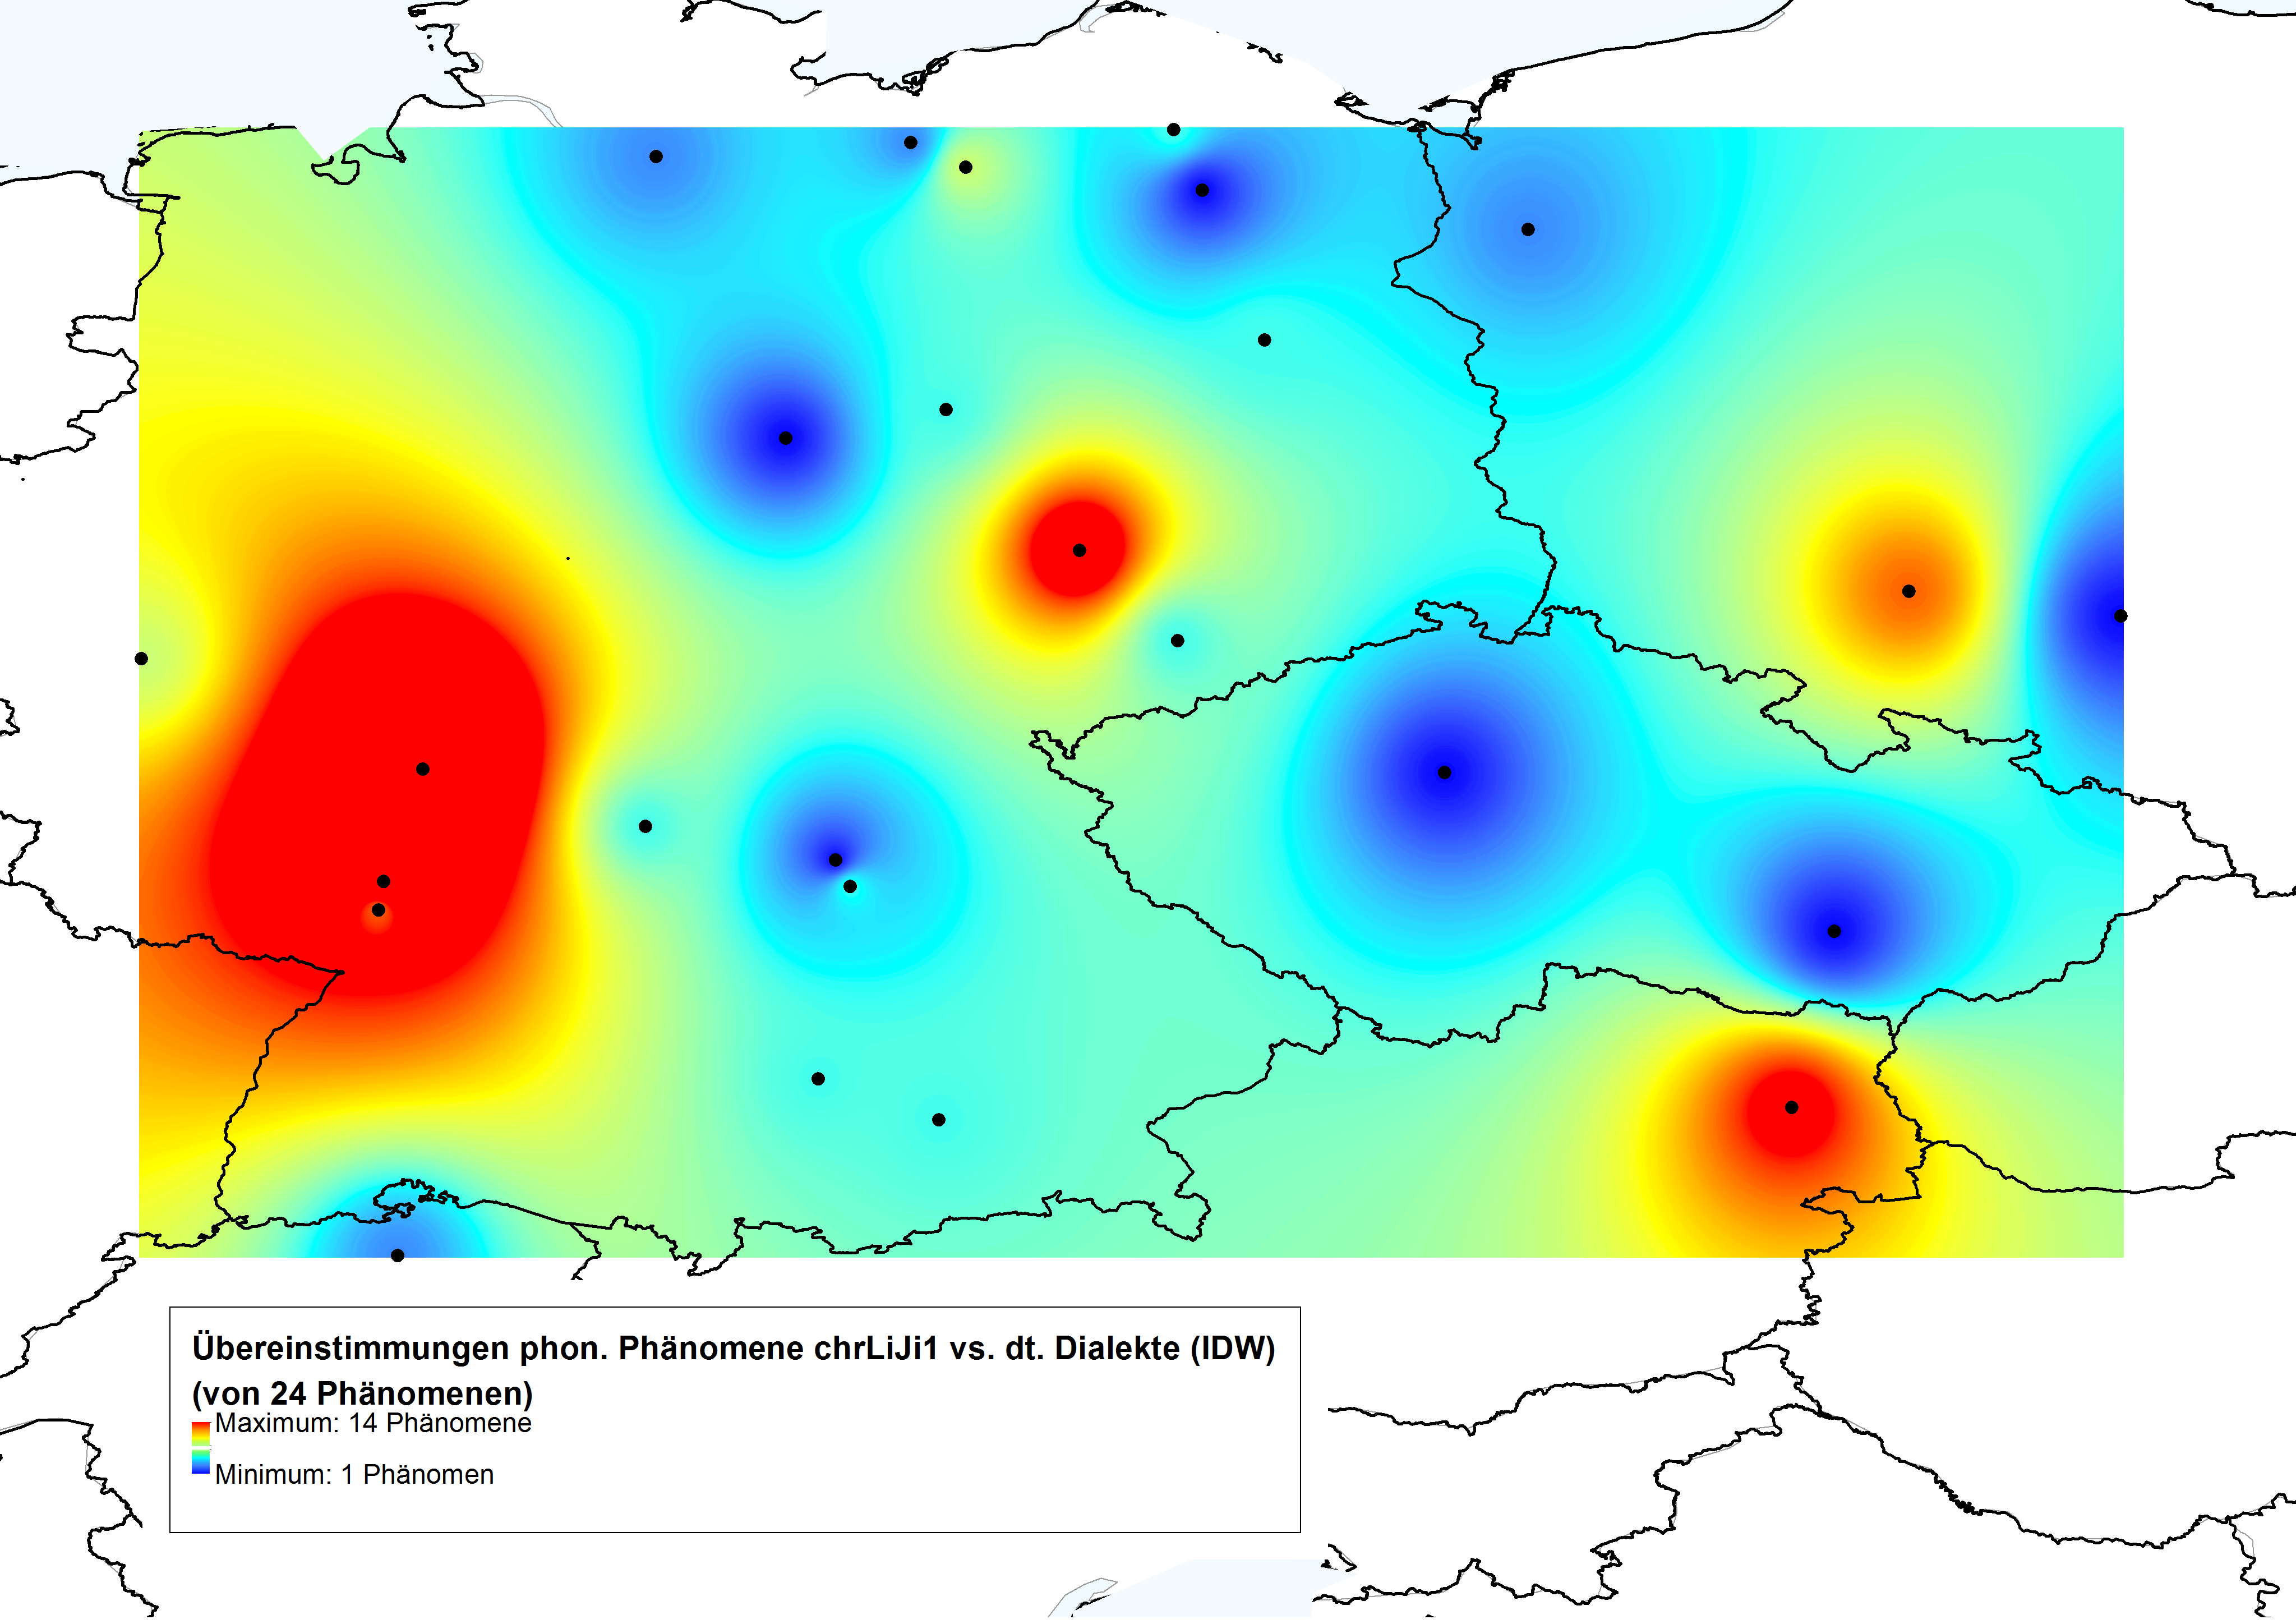
\includegraphics[scale=0.42]{figures/Uebereinstimmung_phon_liji_dnurIDW_PUNKT.png}
		\caption{\label{IDWallphondtliji} Gemeinsame phonologische Phänomene des \hai{chrLiJi1} und der entsprechenden dt. Dialekte (\hai{IDW})}
		\end{figure}
\FloatBarrier
  
 Die Karte \ref{allphonnegIDW} stellt hingegen dar, wo besonders viele bzw. wenige phonologische Markierungen im \hai{chrLiJi1} auftreten, die im Ortsdialekt nicht gegeben sind. Die Differenz zwischen deutschem Dialekt und \hai{chrLiJi1} ist v.\,a. im Mittelbairischen und Berliner Raum besonders groß. Aber auch im Ripuarischen Bonns und im Mittelbairischen Wiens werden viele ortsfremde Phänomene verwendet.  Weniger auffällig sind die Unterschiede zwischen \hai{chrLiJi1} und deutschem Dialekt im schlesischen, böhmischen, ostpommerschen, alemannischen und rheinfränkischen Raum. \\
 

 \begin{figure}[h!]
		\centering
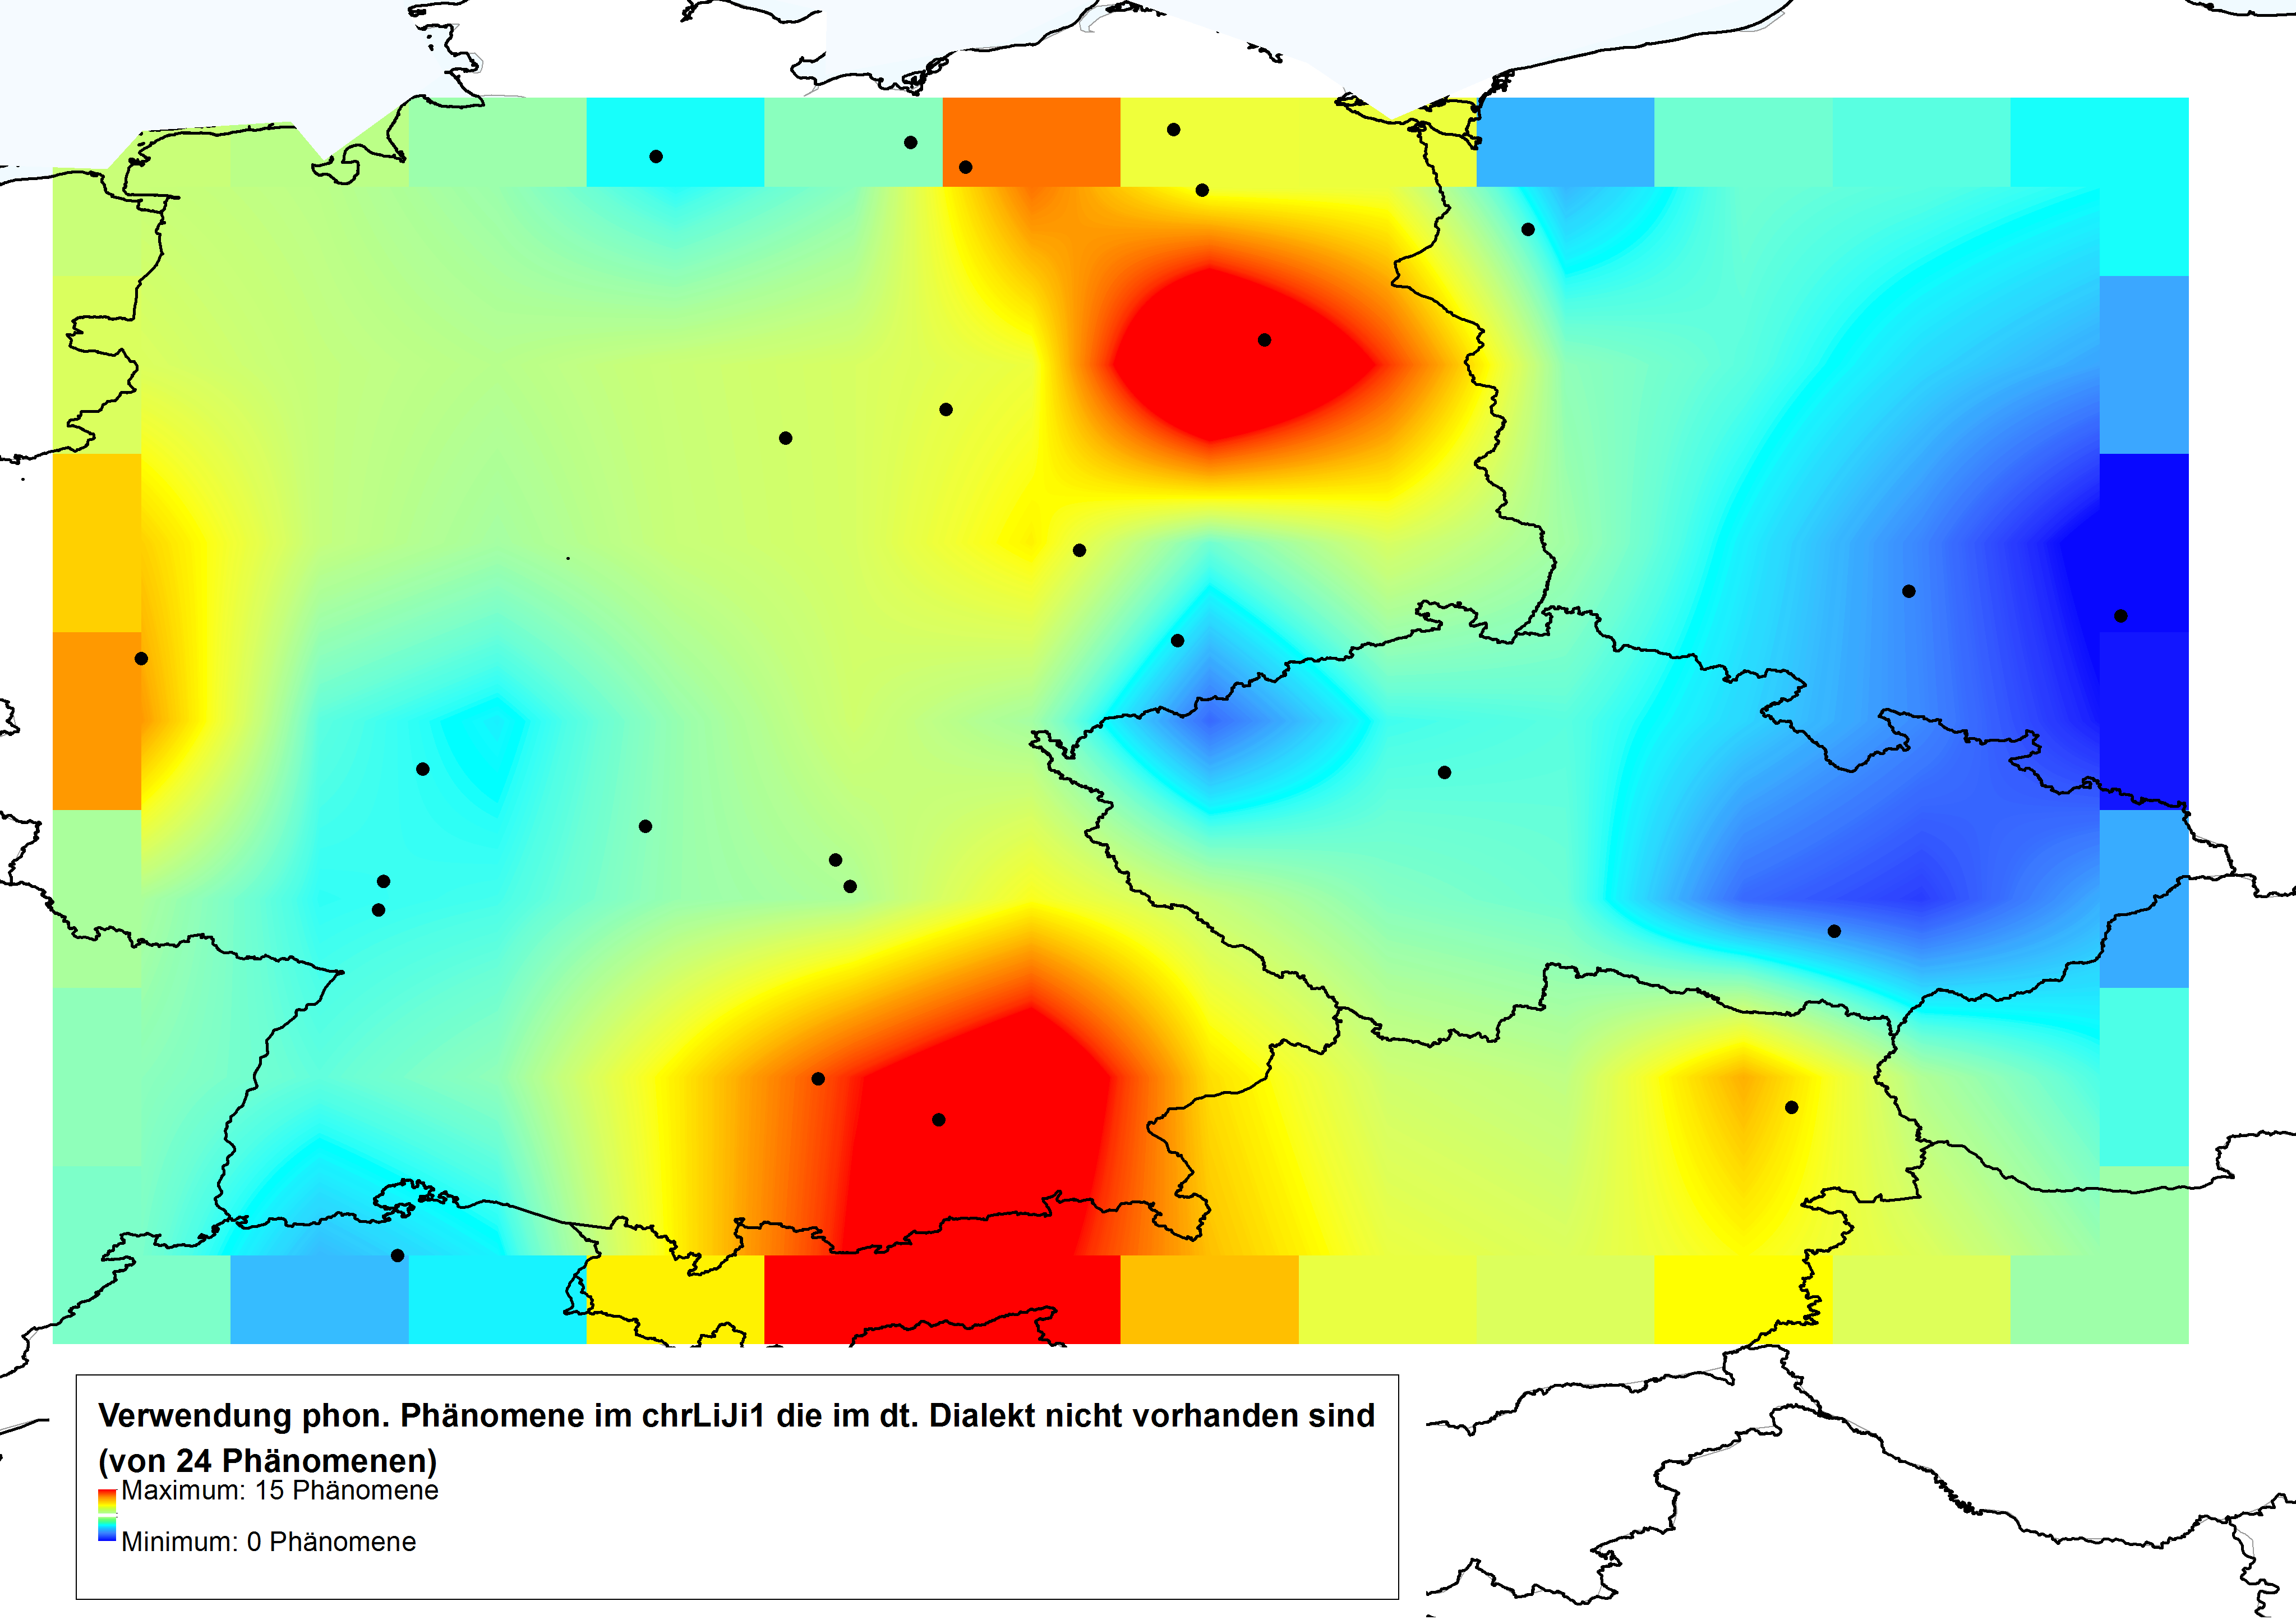
\includegraphics[scale=0.42]{figures/IDW_phon_negativ_dt_liji_PUNKT.png}
		\caption{\label{allphonnegIDW} Ortsfremde phonologische Phänomene des \hai{chrLiJi1} (\hai{IDW})}
		\end{figure}
\FloatBarrier
 
 Aus den Belegdaten zu sieben Phänomenen, die als besonders charakteristisch für das Westjiddische angesehen werden,\footnote{Diese Phänomene sind die Monophthongierung von \hai{V24}, \hai{V44} und deren \isi{Zusammenfall}, die Diphthongierungen von \hai{V22}, \hai{V42} und \hai{V34} sowie der Erhalt von germ. -\textit{pp}-.} ist die Karte in Abbildung \ref{westjiddischphonIDW} entstanden. Man sieht in der \hai{IDW} deutlich, dass westjiddische Formen besonders stark in den Bonner Quellen, den Texten aus den bairischen und obersächsischen Diealekträumen sowie denen aus Berlin auftreten; seltener aber im Niederdeutschen, Schlesischen, Böhmischen, Mährischen, Südbairischen, sprich im äußersten Osten des Untersuchungsgebiets. Das \hai{chrLiJi1} entspricht somit erstaunlicherweise dem Gebiet des Übergangsjiddischen, wo wir bereits ostjiddische Formen annehmen dürfen. Dies gilt zwar nicht für den äußersten Norden, wo wir auf niederdeutschem Gebiet eine Zahl an Quellen finden, in denen westjiddische Formen kaum auftreten. Auffällig verhalten sich auch die rheinfränkischen Quellen (Speyer, Mannheim, Frankfurt), die nur sehr wenige der ausgewählten westjiddischen Phänomene aufweisen, und dies obwohl sie in den örtlichen deutschen Dialekten beinahe alle gegeben sind (vgl. Abb. \ref{allphonnegIDWdeutsch}). Hier kann angenommen werden, dass gerade um die Distanz zum örtlichen Dialekt herzustellen, auf charakteristische westjiddische Phänomene (zugunsten anderer) verzichtet wurde. Da es sich bei den Quellen um Theaterstücke handelt, welche besonders regional für die örtlichen Theater geschrieben wurden (insbes. im Fall der Mannheimer Quellen), ist eine erkennbare Unterscheidung zwischen jüdischem und deutschem Dialekt besonders wichtig an Orten, an denen die Gemeinsamkeiten besonders stark sind.\\

 
  \begin{figure}[h!]
		\centering
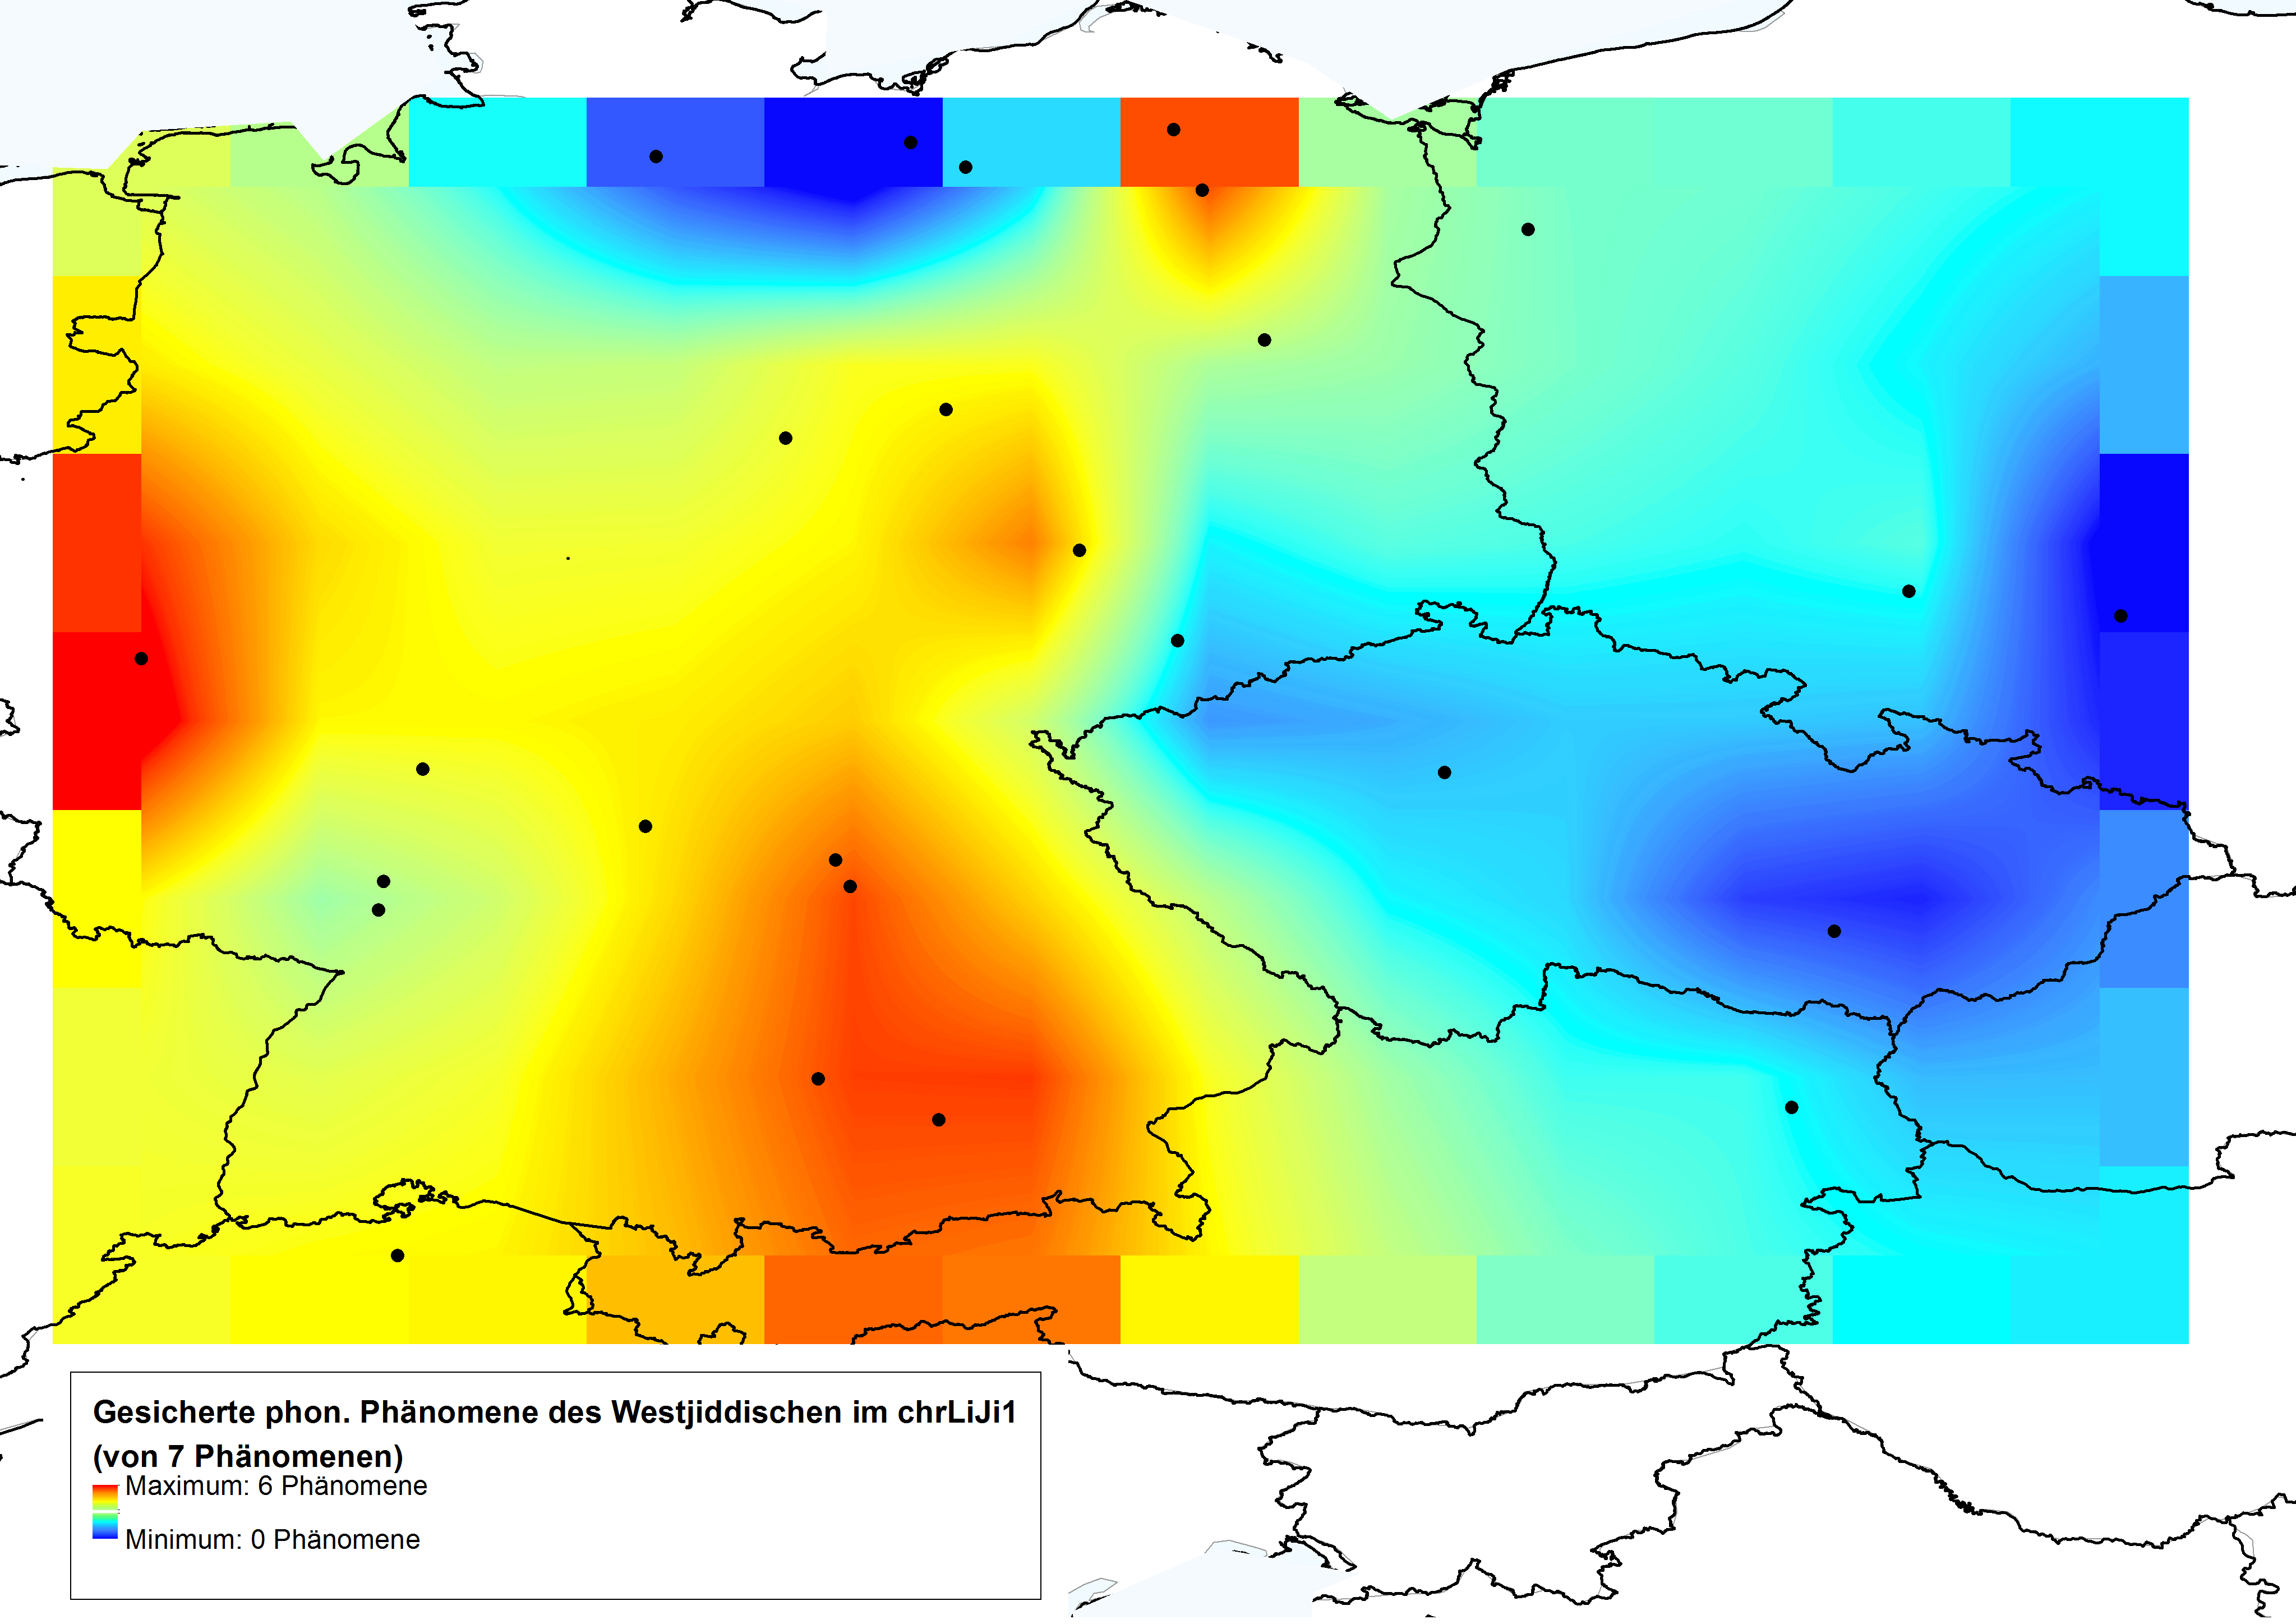
\includegraphics[scale=0.42]{figures/westjiddischPHON_IDW_PUNKT.png}
		\caption{\label{westjiddischphonIDW} Westjiddische phonologische Phänomene im \hai{chrLiJi1} (\hai{IDW})}
		\end{figure}
\FloatBarrier
		 
 Das Kartenbild in Abbildung \ref{allphonnegIDWdeutsch} entspricht in etwa dem aus Abbildung \ref{IDWallphondtliji}. Hier wurden eben jene, auch für die Darstellung in Karte \ref{westjiddischphonIDW} relevanten sieben besonders idiosynkratischen Phänomene des \hai{WJ} herangezogen. Der Vergleich zwischen der Verteilung westjiddischer Phänomene in den deutschen Dialekten (Karte in Abb. \ref{allphonnegIDWdeutsch}) und der Verteilung eben dieser Phänomene im \hai{chrLiJi1} (Karte in Abb. \ref{westjiddischphonIDW}) zeigt klare Unterschiede und bestätigt damit, dass die deutschen Dialekte nur sehr geringen Einfluss auf die Manipulationen des \hai{chrLiJi1} haben.\\
 
  \begin{figure}[h!]
		\centering
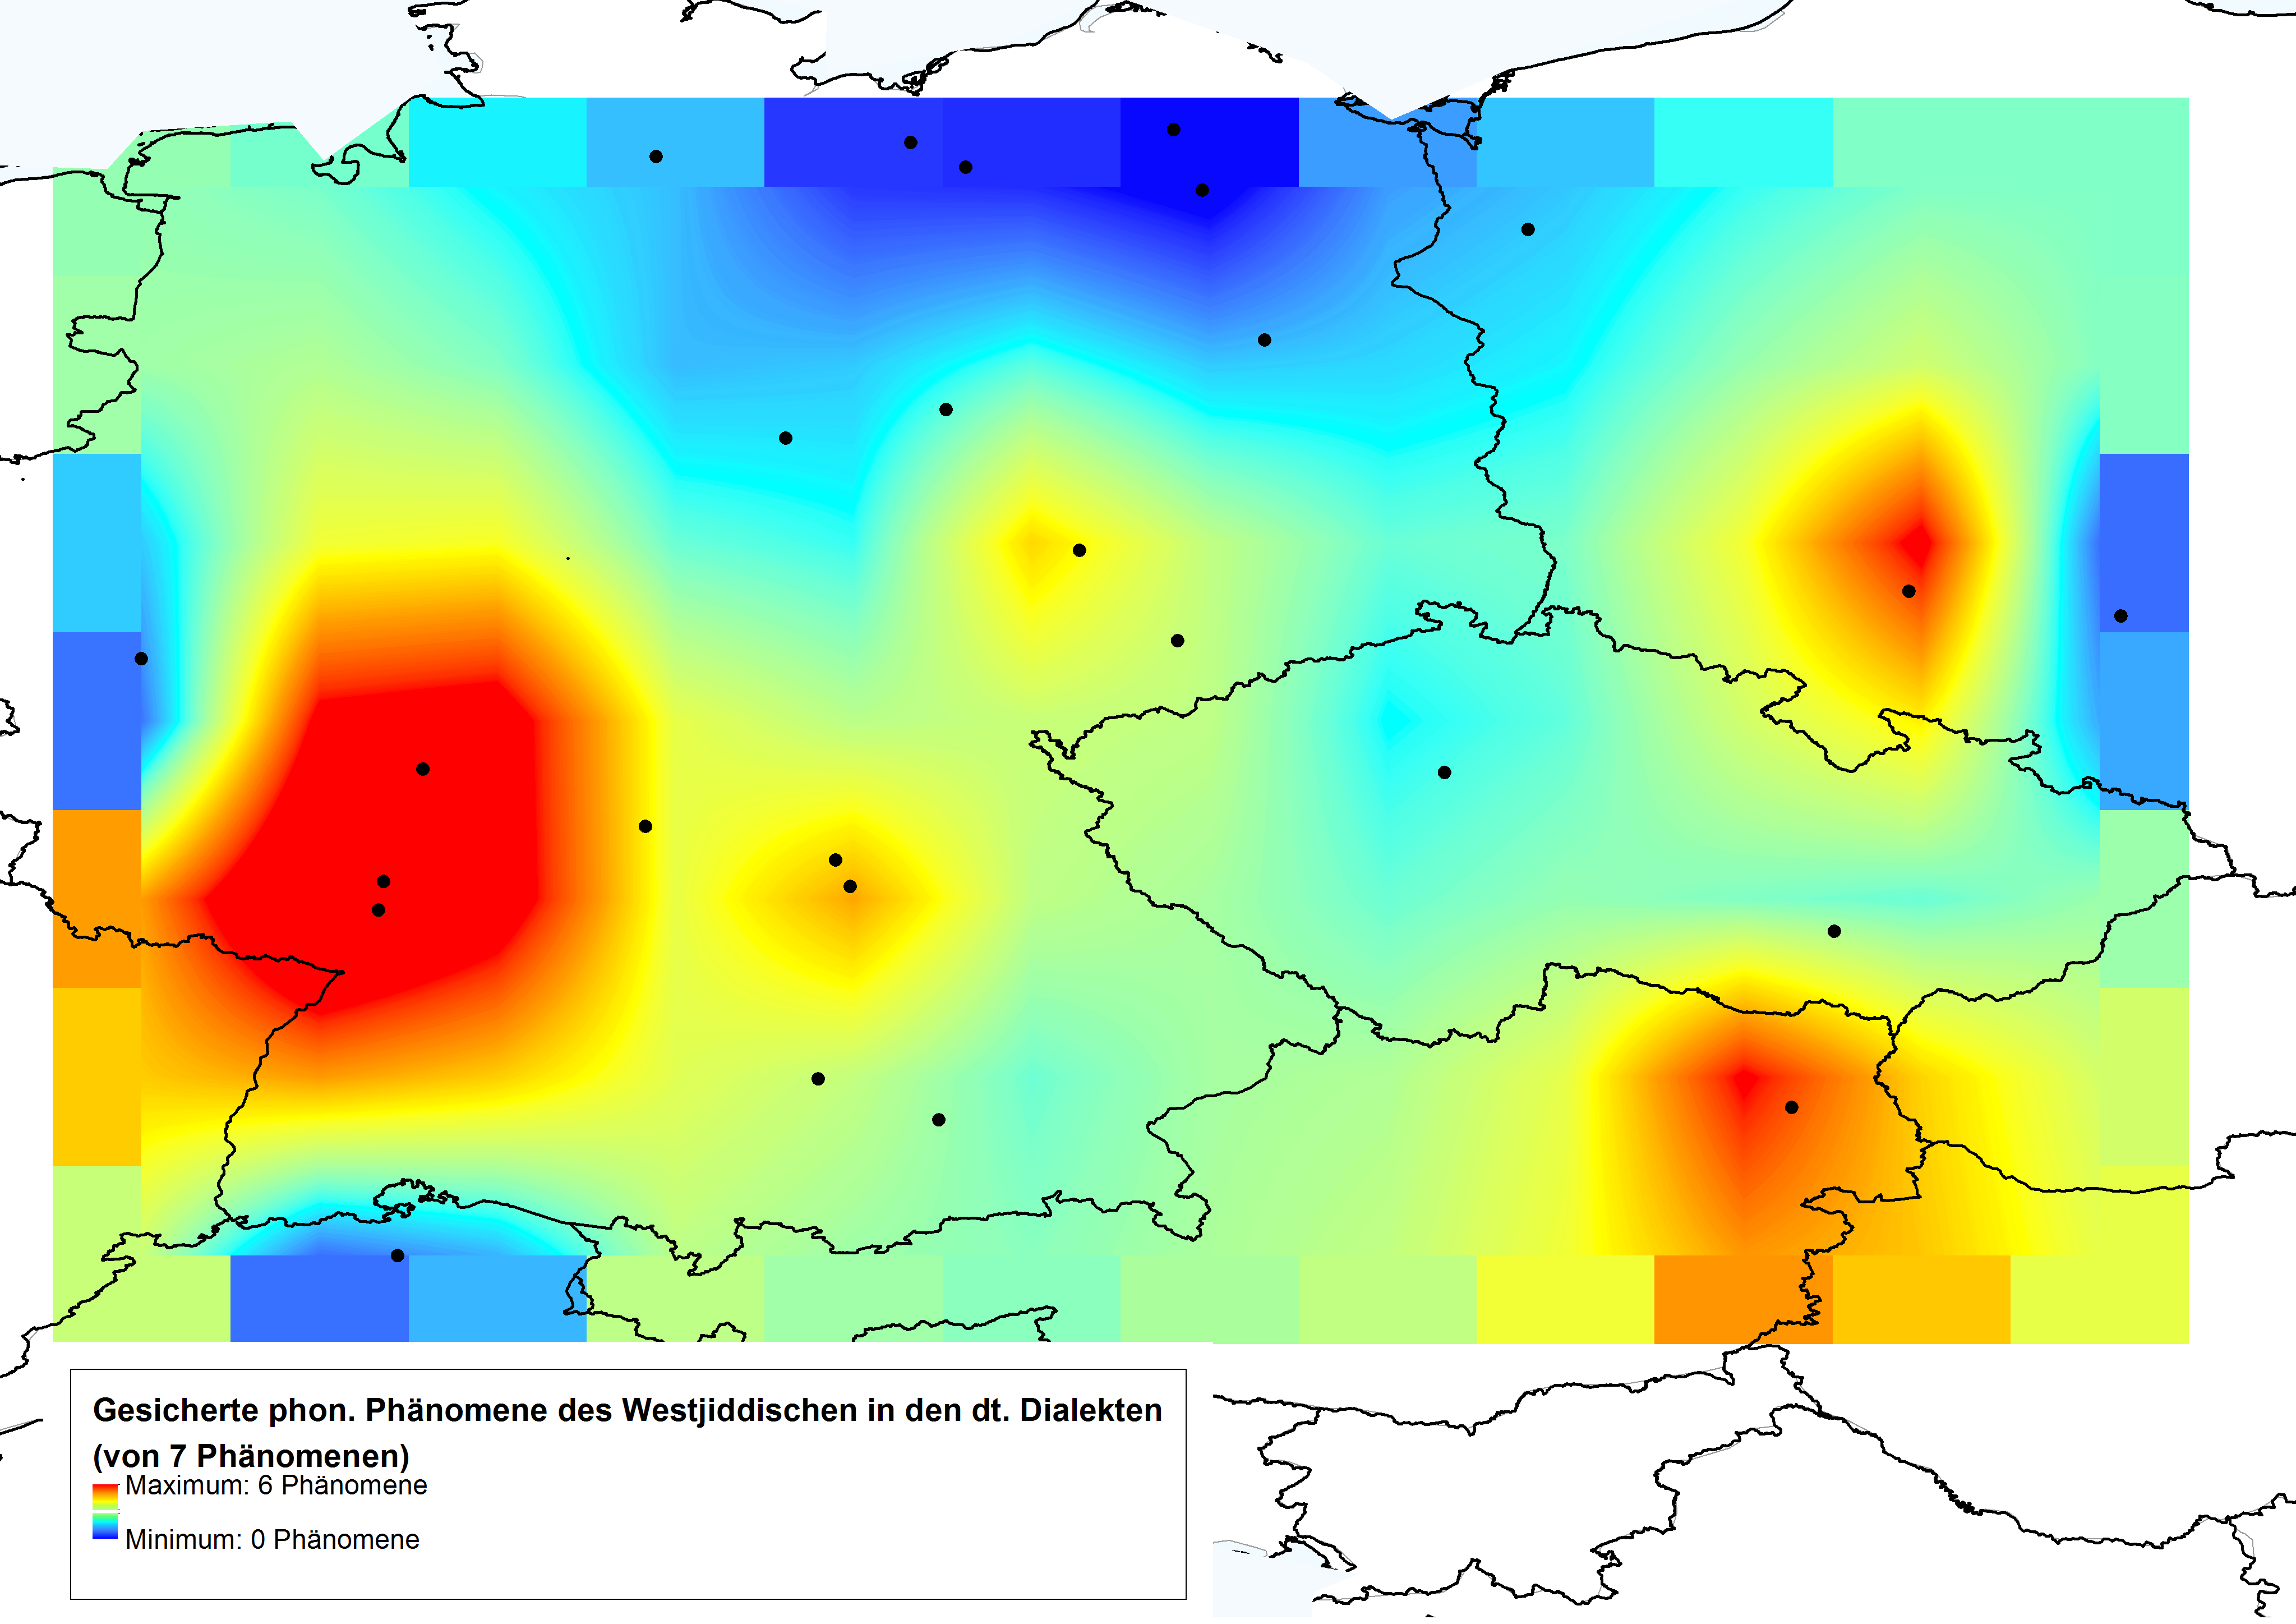
\includegraphics[scale=0.42]{figures/westjiddischPHON_DEUTSCH_IDW_PUNKT.png}
		\caption{\label{allphonnegIDWdeutsch} Westjiddische phonologische Phänomene des \hai{chrLiJi1} in den dt. Dialekten (\hai{IDW})}
		\end{figure}
\FloatBarrier
  
 Der Vergleich zu literarischen Quellen jüdischer Autoren (\hai{jüdLiJi1}) hat ergeben, dass die Autorschaft im Grunde keinen entscheidenen Einfluss auf die verwendeten Strategien nimmt; z.\,T. sind die Quellen christlicher Autoren sogar ergiebiger als die jüdischer. \\	
 
 
  \chapter{Morphologische Markierungen}\label{morphologie}
 %\noindent
Im Bereich der \isi{Morphologie} weist das \hai{LiJi} weit weniger Strategien zur \isi{Emulation} des Jiddischen auf, als es auf phonologischer Ebene der Fall ist. Selbst wenn die Quellen quantitativ nur wenige Manipulationen an der \isi{Morphologie} vornehmen, ist diese nicht minder interessant. So zeigen etwa einige der morphologischen Phänomene interessante diachrone Streuungen. In der Analyse der 53 untersuchten Quelltexte sind von der Schriftnorm abweichende Auffälligkeiten bezüglich Nominal- (Genuswahl, \isi{Diminution}, Pluralbildung, Kasussystem) und Verbalmorphologie (Flexionsformen, \isi{Wortakzent} bei Präfix-/Partikelverben) zu verzeichnen. Diese gilt es im Folgenden im Einzelnen darzulegen. \\


 \section{Genusverschiebungen}\label{genus}
%\noindent
 Einige Quellen des \hai{chrLiJi1} und \hai{jüdLiJi} zeigen den Gebrauch abweichender Genera. Die Genuszuweisung im Standardjiddischen entspricht (bei den Lexemen der germanischen Komponente) weitestgehend dem Deutschen (vgl. \cite[166–168]{Jacobs2005}). Es gibt einige Ausnahmen, wo Variationen zwischen den drei Genera Femininum, Maskulinum und Neutrum im Standardjiddischen vorliegen, die im Deutschen nicht gegeben sind, z.\,B. in \ref{BELEGEGENJI}. Es sind besonders Feminina, die zum maskulinen \isi{Genus} wechseln können. Ausnahmen wie in \ref{bspWEIB} lassen sich mit semantischer Kongruenz (\textit{Dehybridisierung}) erklären (vgl. \cite{Fleischer2012}). Weitere Unterschiede zum deutschen Genussystem finden sich bei jüngeren Lexemen, wie z.\,B. \ref{bspHP}. Im Genussystem liegt sicherlich eine der größten Diskrepanzen zwischen Standard und gesprochener Sprache vor (\cite[insbes. 153–207]{Wolf1969}). \label{GENUSNOJ}Dialektale Variation findet sich besonders im \hai{NOJ}, wo im Unterschied zu den übrigen jiddischen Varietäten das Neutrum abgebaut und ein Genussystem entwickelt wurde, welches nur noch die Opposition \quein{maskulin–feminin} besitzt (vgl. \cite{Jacobs1990b}; \cite{Wolf1969}; \cite[101–124]{Herzog1965}). In den Dialekten des \hai{NOJ} und \hai{SOJ} finden sich darüber hinaus auch Wechsel historischer Feminina zu Maskulina (\cite[160–168]{Wolf1969}) bzw. von Maskulina zu Feminina (\cite[168–176]{Wolf1969}). In manchen Lexemen können sogar alle drei Genera in den Dialekten auftreten, wie z.\,B. in \ref{bspRAD}  (vgl. \cite[178]{Wolf1969}). Eine Abweichung vom schriftdeutschen Genussystem im \hai{LiJi} könnte auf diese ostjiddischen Dialektsysteme verweisen. \\
 
  \eenumsentence{\label{BELEGEGENJI}
\item  \RL{דער/דיע מויער} \textit{der/di moyer} \sem{die Mauer} (zitiert n.\cite[167]{Jacobs2005})
 
\item  \RL{דער/דיע נוס} \textit{der/di nus} \sem{die Nuss}

\item  \RL{דער/דיע גרענעץ} \textit{der/di grents} \sem{die Grenze}

\item  \RL{דאָס/דיע וו{יי}\makebox(-1.5,-7.5)[r]{\libertineGlyph{uni207B}}ב} \textit{dos/di vayb} \sem{die Frau} (zitiert n. \cite[167]{Jacobs2005}) \label{bspWEIB}

\item  \RL{דאָס/דער  וועבבלא\makebox(-1.5,-7.5)[r]{\libertineGlyph{uni207B}}ט} \textit{dos/der vebblat} \sem{die Homepage}  \label{bspHP}


\item  \RL{דאָס  ראָד} \textit{dos rod} (südl. \hai{ZOJ}) – \RL{דער  ראָד} \textit{der rod} (\hai{NOJ}) –  \RL{דיע  ראָד} \textit{die rod} (\hai{SOJ}) \sem{das Rad}(zitiert n. \cite[178]{Wolf1969})
 \label{bspRAD} 
  } 
 
  Diese Form der dialektalen Variation im Ostjiddischen lässt sich bis zu einem gewissen Grad auf den Einfluss, den osteuropäische Sprachen auf das Jiddische ausgeübt haben, zurückführen (vgl. \cite{Trudgill1999}; \cite[591]{Weinreich1973}). 
So sind Genus-Mismatches ein häufiges Phänomen intensiven Sprachkontakts (vgl. \cite{Trudgill1999}). Dies gilt besonders in den modernen germanischen Sprachen, wo die Genuszuweisung nicht (mehr) ersichtlich ist. Genusschwankungen und \isi{Genus}übergänge sind aber auch für die Diachronie und Diatopie des Deutschen reichlich belegt (\cite[443f]{Schirmunski1962}). Ein Einfließen deutsch-dialektaler Formen auf das \hai{chrLiJi1} ist somit nicht völlig von der Hand zu weisen (vgl. Bsp. \ref{BSPGENUS_6}). Möglich wäre aber auch eine rein literarische Funktion der Genusverstöße an der deutschen Schreibvarietät. So kann besonders die Verwendung des Neutrums bei Personennamen zu pejorativen Zwecken dienen (vgl. \cite{NueblingimErsch}). Personennamen sind im \hai{LiJi} allerdings kaum von Genusverstößen betroffen. 

Die einzelnen Belege für die Setzung eines abweichenden \isi{Genus} sind in \ref{BELEGEGENUS} aufgeführt.\footnote{Alle diese Belege stehen im Nominativ, eine Kasusalternanz wäre demnach auszuschließen (vgl. Abschnitt \ref{kasus}).} Im \hai{chrLiJi1} finden sich einzelne Belege in sechs Quellen (\ref{BSPGENUS_1}–\ref{BSPGENUS_7}). Das \hai{jüdLiJi1} zeigt einen einzelnen Beleg (\ref{BSPGENUS_8}). Mit Blick auf die pejorative Funktion wäre eine besondere Hervorhebung des Neutrums anzunehmen (vgl. \cite{NueblingimErsch}). Dies ist jedoch nur in zwei Belegen (\ref{BSPGENUS_2} und \ref{BSPGENUS_3}) der Fall, die übrigen sechs Belege wählen das Maskulinum zur Markierung. Dies ist besonders interessant, da in vier dieser sechs Belege ein Neutrum maskulin wird, was ideal in die Strukturen des \hai{NOJ} passen würde (vgl. \cite{Jacobs1990}). Für einen nordostjiddischen Einfluss auf das \hai{LiJi} spricht besonders die geographische Verteilung der Belege: Mit der Ausnahme einer Mannheimer Quelle liegen alle Belege im östlichen Teil des westjiddischen Sprachgebiets (vgl. Abb. \ref{KarteGenus}), wo die direkte Einwanderung von Sprechern des Nordostjiddischen wahrscheinlicher ist, als im Westen bzw. Süden. 
Besonders interessant sind die Belege (\ref{BSPGENUS_1}), (\ref{BSPGENUS_5}), (\ref{BSPGENUS_7}) und (\ref{BSPGENUS_8}), da hier das korrekte ostjiddische \isi{Genus} verwendet wird. Die Autoren müssen hier demnach eine besonders gute Kenntnis vom Ostjiddischen gehabt haben.\\


 \eenumsentence{\label{BELEGEGENUS}
 \item \textit{der Spektakel} \sem{das Spektakel} (\hai{BS:\,4}); vgl. oj. \RL{דער ספּעקטא\makebox(-1.5,-7.5)[r]{\libertineGlyph{uni207B}}קל} \textit{der spektakl}\label{BSPGENUS_1} %M-N %\ili{OJ}

 \item \textit{das Litteratur} \sem{die Literatur} (\hai{HJ:\,97}); vgl. oj. \RL{דיע ליטערא\makebox(-1.5,-7.5)[r]{\libertineGlyph{uni207B}}טור} \textit{di literatur}\label{BSPGENUS_2} %N-F  
 
  \item \textit{das arme Jued} \sem{der arme Jude} (\hai{WA:\,157}); vgl. oj. \RL{דער ייִד} \textit{der yid}\label{BSPGENUS_3}%N-M 

  \item \textit{einen guten Gehalt} \sem{ein gutes Gehalt} (\hai{FM:\,8}); \\
  vgl. oj. \RL{דאָס געהא\makebox(-1.5,-7.5)[r]{\libertineGlyph{uni207B}}לט} \textit{dos gehalt}\label{BSPGENUS_4}%M-N 
    
%  \item \textit{Ihrem Großtante} \sem{Ihre Großtante} (\hai{SS:\,18})\label{BSPGENUS_4.2}
 
  \item \textit{der Schiff} \sem{das Schiff} (\hai{SS:\,18}); vgl. oj. \RL{דיע שיף} \textit{die shif}\label{BSPGENUS_5} 
  %M-N %\ili{OJ}
 
  \item \textit{ein Lerche} \sem{eine Lerche} (\hai{LR:\,11});\\ 
  vgl. Mitteldt. (südmos. Obh.) \textit{der lerx} (\cite[444]{Schirmunski1962}); \\
  oj. \RL{דאָס טרילערל} \textit{dos trillerl} \sem{die Lerche} \label{BSPGENUS_6}
%M-F 

  \item \textit{ein Wachtel} \sem{eine Wachtel} (\hai{LR:\,11}); \\
vgl. oj. \RL{דער ווא\makebox(-1.5,-7.5)[r]{\libertineGlyph{uni207B}}כטל} \textit{der wachtel}\label{BSPGENUS_7} %M-F %\ili{OJ}
  
  
   \item \textit{der großer Seminar} \sem{das große Seminar} (\hai{GuS23:\,4})\\
   vgl. oj. \RL{דער סעמינא\makebox(-1.5,-7.5)[r]{\libertineGlyph{uni207B}}ר} \textit{der seminar}\label{BSPGENUS_8} %jüdLIJI1 %M-N %\ili{OJ}

   
  } 




\begin{figure}[h!]
\centering
\includegraphics[scale=0.5]{figures/Karte\isi{Genus}.png}
		\caption{\label{KarteGenus} Genusverschiebungen im \hai{chrLiJi1}}
	\end{figure}
\FloatBarrier 
	 

Abschließend lässt sich festhalten, dass Genusverschiebungen von der deutschen Schriftsprache im \hai{LiJi1} äußerst selten vorkommen. Die Hälfte der Belege verwenden Genera, die ostjiddischen Formen entsprechen. Dies ist erstaunlich und kann für eine Kenntnis dieser Autoren vom Ostjiddischen sprechen oder als Hinweis für ein vom Schriftdeutschen abweichendes Genussystem im Westjiddischen interpretiert werden. Wie nun die übrigen vier Belege zu interpretieren sind, muss offen bleiben. Zum einen ist es durchaus möglich, dass die entsprechenden Lexeme in den entsprechenden jiddischen Dialekten genau die Genera aufweisen, die im \hai{LiJi1} belegt sind. Andererseits ist auch die pejorative Funktion von Genusverstößen nicht völlig von der Hand zu weisen. 
Plausibel erscheint es, eine Kombination zwischen Pejoration und Sprachrealität anzunehmen. \\


 
  
 \section{Diminutionen}\label{dim}
 %\noindent
Die \isi{Diminution} ist ein äußerst frequentes Mittel der Charakterisierung jüdischer Figuren. Es finden sich im \hai{chrLiJi1} in 39 (von 53) Quellen 12 verschiedene Diminutivsuffixe für die Singulardiminution (Tabelle \ref{tblDIMSG}, S. \pageref{tblDIMSG}) und in 27 Texten 14 Suffixe für die \isi{Diminution} im Plural (Tabelle \ref{tblDIMPL}, S. \pageref{tblDIMPL}). In vielen Texten werden dabei mehrere Suffixe parallel verwendet. Im Singular zeigen 14 Quellen zwei unterschiedliche Suffixe parallel. Insgesamt sieben Quellen verwenden drei und in jeweils einer Quelle treten vier (\hai{PA} Frankfurt, 1834) und sechs (\hai{GW} n.a., ca. 1900) unterschiedliche Suffixe nebeneinander auf. Der Mittelwert liegt bei 1,4 Suffixen pro Quelle (bei einer Standardabweichung von 1,2). Sechs Quellen verwenden zwei unterschiedliche Suffixe zur Pluraldiminution; fünf Quellen drei und eine Quelle (\hai{PG} Speyer, 1835) vier Suffixe. Dies allein zeigt, welche Vielzahl an Suffixen eingesetzt wird.\label{AnzahlDIM}

Die im Jiddischen verwendeten Diminutivsuffixe entstammen der germanischen Komponente. Aus diesem Grund wird, bevor auf die \isi{Diminution} im Jiddischen eingegangen wird (Unterabschnitt \ref{dimJIDDISCH}), das deutsche System dargestellt (Unterabschnitt \ref{dimDEUTSCH}). Da das Jiddische die Unterscheidung zwischen Diminutivsingular und -plural trifft (\cite[162–166]{Jacobs2005}), erfolgt die anschließende Analyse aufgrundlage dieser Trennung. Es werden zunächst die einzelnen im \hai{LiJi} vorfindbaren Singulardiminutiva  und später die Pluraldiminutiva dargestellt und mit der Situation im Jiddischen und den deutschen Dialekten verglichen. In die Analyse nicht aufgenommen wird die semantische Kategorie des Diminutivs 1. und 2. Grades, der eine Unterscheidung zwischen \sem{verkleinernd} und \sem{verzärtlichend} trifft und für das Jiddische angenommen wird (\cite[48]{Landau1895}; \cite[80]{Perlmutter1988}; \cite[162]{Jacobs2005}),\footnote{Eine solche semantische Differenzierung ist auch aus den deutschen Dialekten bekannt, wie z.\,B. dem Schwäbischen oder dem Hochalemannischen (vgl. \cite[1250]{Seebold1983}; \cite[159–208]{Luessy1974}; \cite[162]{Schirmunski1962}).} da solche Kategorien bestenfalls durch direkte Sprecherbefragung, aber nur schwer aufgrundlage schriftlicher Quellen ermittelt werden können.\\





\subsection{\isi{Diminution} in den deutschen Dialekten}\label{dimDEUTSCH}
%  %\noindent
Im Deutschen wie auch im Jiddischen erfolgt die \isi{Diminution} mittels Umlautung des Stammvokals und Suffigierung am Stamm. Für die Dialekte des Deutschen veranschlagt man abhängig vom Konsonanten des Suffixes eine grobe Einteilung in \hai{L}- und \hai{K}-\isi{Diminution} (u.\,a. \cite{Wrede1908}; \cite[475–487]{Schirmunski1962}; \cite{Seebold1983}), d.\,h. es liegen zwei Klassen von Diminutivsuffixen vor, die sich in ihrem Basiskonsonanten unterscheiden. Dabei finden sich Diminutivformen mit -\textit{l}- als Basiskonsonant im Süden des Sprachgebiets, Formen auf -\textit{k}-(> -\textit{ch}-) im Norden (vgl. Abb. \ref{tblDIMsystemSg}, S. \pageref{tblDIMsystemSg} u. \ref{DimDSA}, S. \pageref{DimDSA}).\footnote{In den dt. Dialekten der Schweiz und Österreichs, die nicht von den Wenkerkarten abgedeckt sind, setzt sich das \isi{Dialektkontinuum} fort und wir finden hier konsequent \hai{L}-\isi{Diminution}.} Diese Nord-Süd-Teilung der Dialekte spiegelt sich selbst im Schriftdeutschen wieder, wo zwei Diminutivsuffixe -\textit{chen} und -\textit{lein} gebräuchlich sind.\footnote{Mittlerweile hat sich überwiegend die ursprünglich ostmitteldeutsche Diminutivbildung mittels -\textit{chen} durchgesetzt (\cite[475, 479]{Schirmunski1962}; \cite[157]{Koenig1978}). Sobald der Stamm auf -\textit{ch}, -\textit{g}, oder -\textit{ng} auslautet, findet sich in der nhd. Schriftsprache die ursprünglich oberdeutsche Bildung mit -\textit{lein} (\cite[475]{Schirmunski1962}).} Die deutschen Mundarten weisen hingegen weitaus mehr und \qu{seit langem konkurrierende Typen von Diminutivformen} auf, als die Standardsprache vermuten lässt (\cite[476]{Schirmunski1962}). Wie \textcite{Wrede1908} in seiner umfassenden Beschreibung der im Wenkermaterial erhobenen Diminutiva zeigt, ist das Auftreten eines Diminutivsuffixes in den meisten Dialekten abhängig von der \isi{Semantik} eines Lexems und dessen phonologischen Bedingungen. Tatsächlich verwenden die meisten Sprecher eines deutschen Dialekts mehr als nur ein Suffix. Die Leitformenkartierung des \hai{WA} ist damit bei diesem Phänomen stark an das einzelne Lexem gebunden (\cite[74f]{Wrede1908}).\label{wredeDIM} Das heißt auch, dass alle nachfolgenden Kartenbilder, insbesondere die Polygone des \hai{WA}, wie auch im Fall der phonologischen Karten, nur die Variationen eines Lexems darstellen und keine Gesetzmäßigkeiten reflektieren (vgl. \cite[79]{Wrede1908}). 
   
   
  Die zwei Basistypen von \isi{Diminution} bewirken je nach Vokal kleinräumige areale Variation. Hinzu kommen Fusionsformen beider Basistypen, wie man sie im mitteldeutschen Raum, also in der Kontaktzone zwischen \hai{L}- und \hai{K}-\isi{Diminution}, findet. Eine Zusammenfassung der belegten Kombinationen findet sich in Tabelle \ref{tblDIMsystemSg} (S. \pageref{tblDIMsystemSg}) für die Singulardiminution und in Tabelle \ref{tblDIMsystem} (S. \pageref{tblDIMsystem}) für die Pluralformen.  
 
	Eine Trennung zwischen Singular- und Pluraldiminution, wie sie das Jiddische zeigt und welche nach den Regeln der morphologischen Natürlichkeit besondere \textit{Ikonizität} abbildet (vgl. \cite[insbes. 98–102]{Mayerthaler1981}; \cite[insbes. 59]{Wurzel1984}), kennen nur wenige deutsche Dialekte. Ausgehend von der in Tabelle \ref{tblDIMsystem} (S. \pageref{tblDIMsystem}) aufgeführten Typisierung werden in Abbildung \ref{DimDSA}  die Einzelformen (\hai{WA}-Karte Nr. 381) zur Pluraldiminution zu entsprechenden Polygonen zusammengefasst, die die einzelnen Typen und ihre räumliche Verbreitung darstellen.\footnote{Das Suffix \textit{-chen} verhält sich in der Typisierung als Pluraldiminutivsuffix problematisch, da es zum einen dem Typ einfacher \hai{K}-\isi{Diminution} zugerechnet werden kann. Gesetzt den Fall es bestünde aus dem Diminutivsuffix \textit{-chen-} zuzüglich einem  \textit{-en}-Plural ist es zum anderen aber auch dem Typ \hai{K}+\hai{Pl.} zuzurechnen. Der Vergleich der Karten zum Singular- und \isi{Pluralsuffix} im \hai{WA} (Karten 381 u. 440) zeigt, dass im ostmitteldeutschen (insbes. dem Obersächsischen) \textit{-chen} sowohl als übliches Suffix zur Singular- als auch zur Pluraldiminution vorliegt. Damit ist keine Unterscheidung zwischen Singular und Plural bei der \isi{Diminution} erkennbar und das Suffix muss hier  zum einfachen \hai{K}-Typ gerechnet werden. Anders sieht es jedoch im Rheinfränkischen (insbes. zwischen Aschaffenburg u.  Weinheim) aus. Hier finden sich im Singular die Suffixe \textit{-che}, \textit{-elche}, \textit{-el} und \textit{-la}. Wir haben es also mit einer äußerst vielfältigen Region von Diminutivsuffixen im Singular zu tun. Im Plural aber findet sich hier flächendeckend \textit{-chen}. Damit unterscheidet sich das Suffix eindeutig vom Singular und die Analyse des Suffix als \hai{K}-\isi{Diminution} + \hai{Pl.}-Suffix erscheint hier sinnvoll, zumindest gilt dies für die Gebiete, in denen \textit{-che} und \textit{-elche} im Singular vorliegen. Aus diesem Grund wurde das entsprechende Gebiet im Rheinfränkischen in Karte \ref{DimDSA} zum \hai{K}+\hai{Pl.}-Gebiet gezählt, während das Gebiet im Obersächsischen, welches \textit{-chen} im Singular und im Plural aufweist, als zur reinen \hai{K}-\isi{Diminution} gehörig kartiert wurde.} Augenscheinlich ist die aus der Singulardiminution bekannte Nord-Süd-Teilung in \hai{K}- und \hai{L}-\isi{Diminution} (vgl. Abb. \ref{SgDimDSA}). Ebenfalls fällt auf, dass eine besondere Pluralmarkierung vor allem in Regionen von \hai{K}-Singulardiminution und besonders im (west-)mitteldeutschen Gebiet verwendet wird. Im Süden hingegen, wo die \hai{L}-\isi{Diminution} verbreitet ist, wird kaum zwischen Plural und Singular am Diminutivum unterschieden. Die Kombination von \hai{L}-\isi{Diminution} im Singular und \hai{K + Pl.}-\isi{Diminution} im Plural, wie sie im Jiddischen vorliegt, ist eine seltene Ausnahme im deutschen Dialektverbund. Lediglich in den Randgebieten des Rhein- und Ostfränkischen kann man  die auf \hai{L}-\isi{Diminution} aufbauenden Pluraldiminutivsuffixe finden und hierbei unter anderem auch das aus dem Jiddischen bekannte Suffix \textit{-lich}. Dieses Suffix findet sich entlang der Isoglosse von \hai{L}- und \hai{K}-Diminutionstypen. Es ist v.\,a. diese geolinguistische Verortung, die dafür spricht, in dem Suffix eine Fusion der beiden Basistypen von \isi{Diminution} zu sehen, wie sie auch bei anderen Suffixen entlang der \hai{L}/\hai{K}-Isoglosse zu finden ist.\footnote{So wird der Fusionscharakter von Diminutivsuffixen im Mitteldeutschen deutlicher am Beispiel des Suffixes \textit{-elcher}, welches als eine Fusion aus \textit{-el}\textsubscript{\hai{L}-Dim.} + \textit{-ch(e)}\textsubscript{\hai{K}-Dim.} + \textit{-(e)r}\textsubscript{Pl.} zu analysieren ist.} \\
	
	
	
	 
  
  \begin{table}[h!]
%\begin{longtable}{ccc|ccc}
\centering
		\begin{tabular}{ll}

		\hline 

\textbf{Muster} &\textbf{Beispiel} (\sem{Ente\textsubscript{Dim. Sg.}})  \\ \hline 

\hai{K} & \textit{-che} \textit{Entche}, \textit{-ke} \textit{Entke} \\
\hai{L} & \textit{-le} \textit{Entla}, \textit{-ile} \textit{Entile} \\

\hai{L + K }& \textit{-elche} \textit{Entelche} \\
  \hline 
 \end{tabular}
		 \caption{Grundmuster von Singulardiminutivsuffixen im Deutschen (basierend auf \hai{WA} Karte Nr. 440 \sem{Stückchen})}
		 \label{tblDIMsystemSg}
		 \end{table}
		% \end{longtable}
 

	
	  \begin{figure}[h!]
\centering
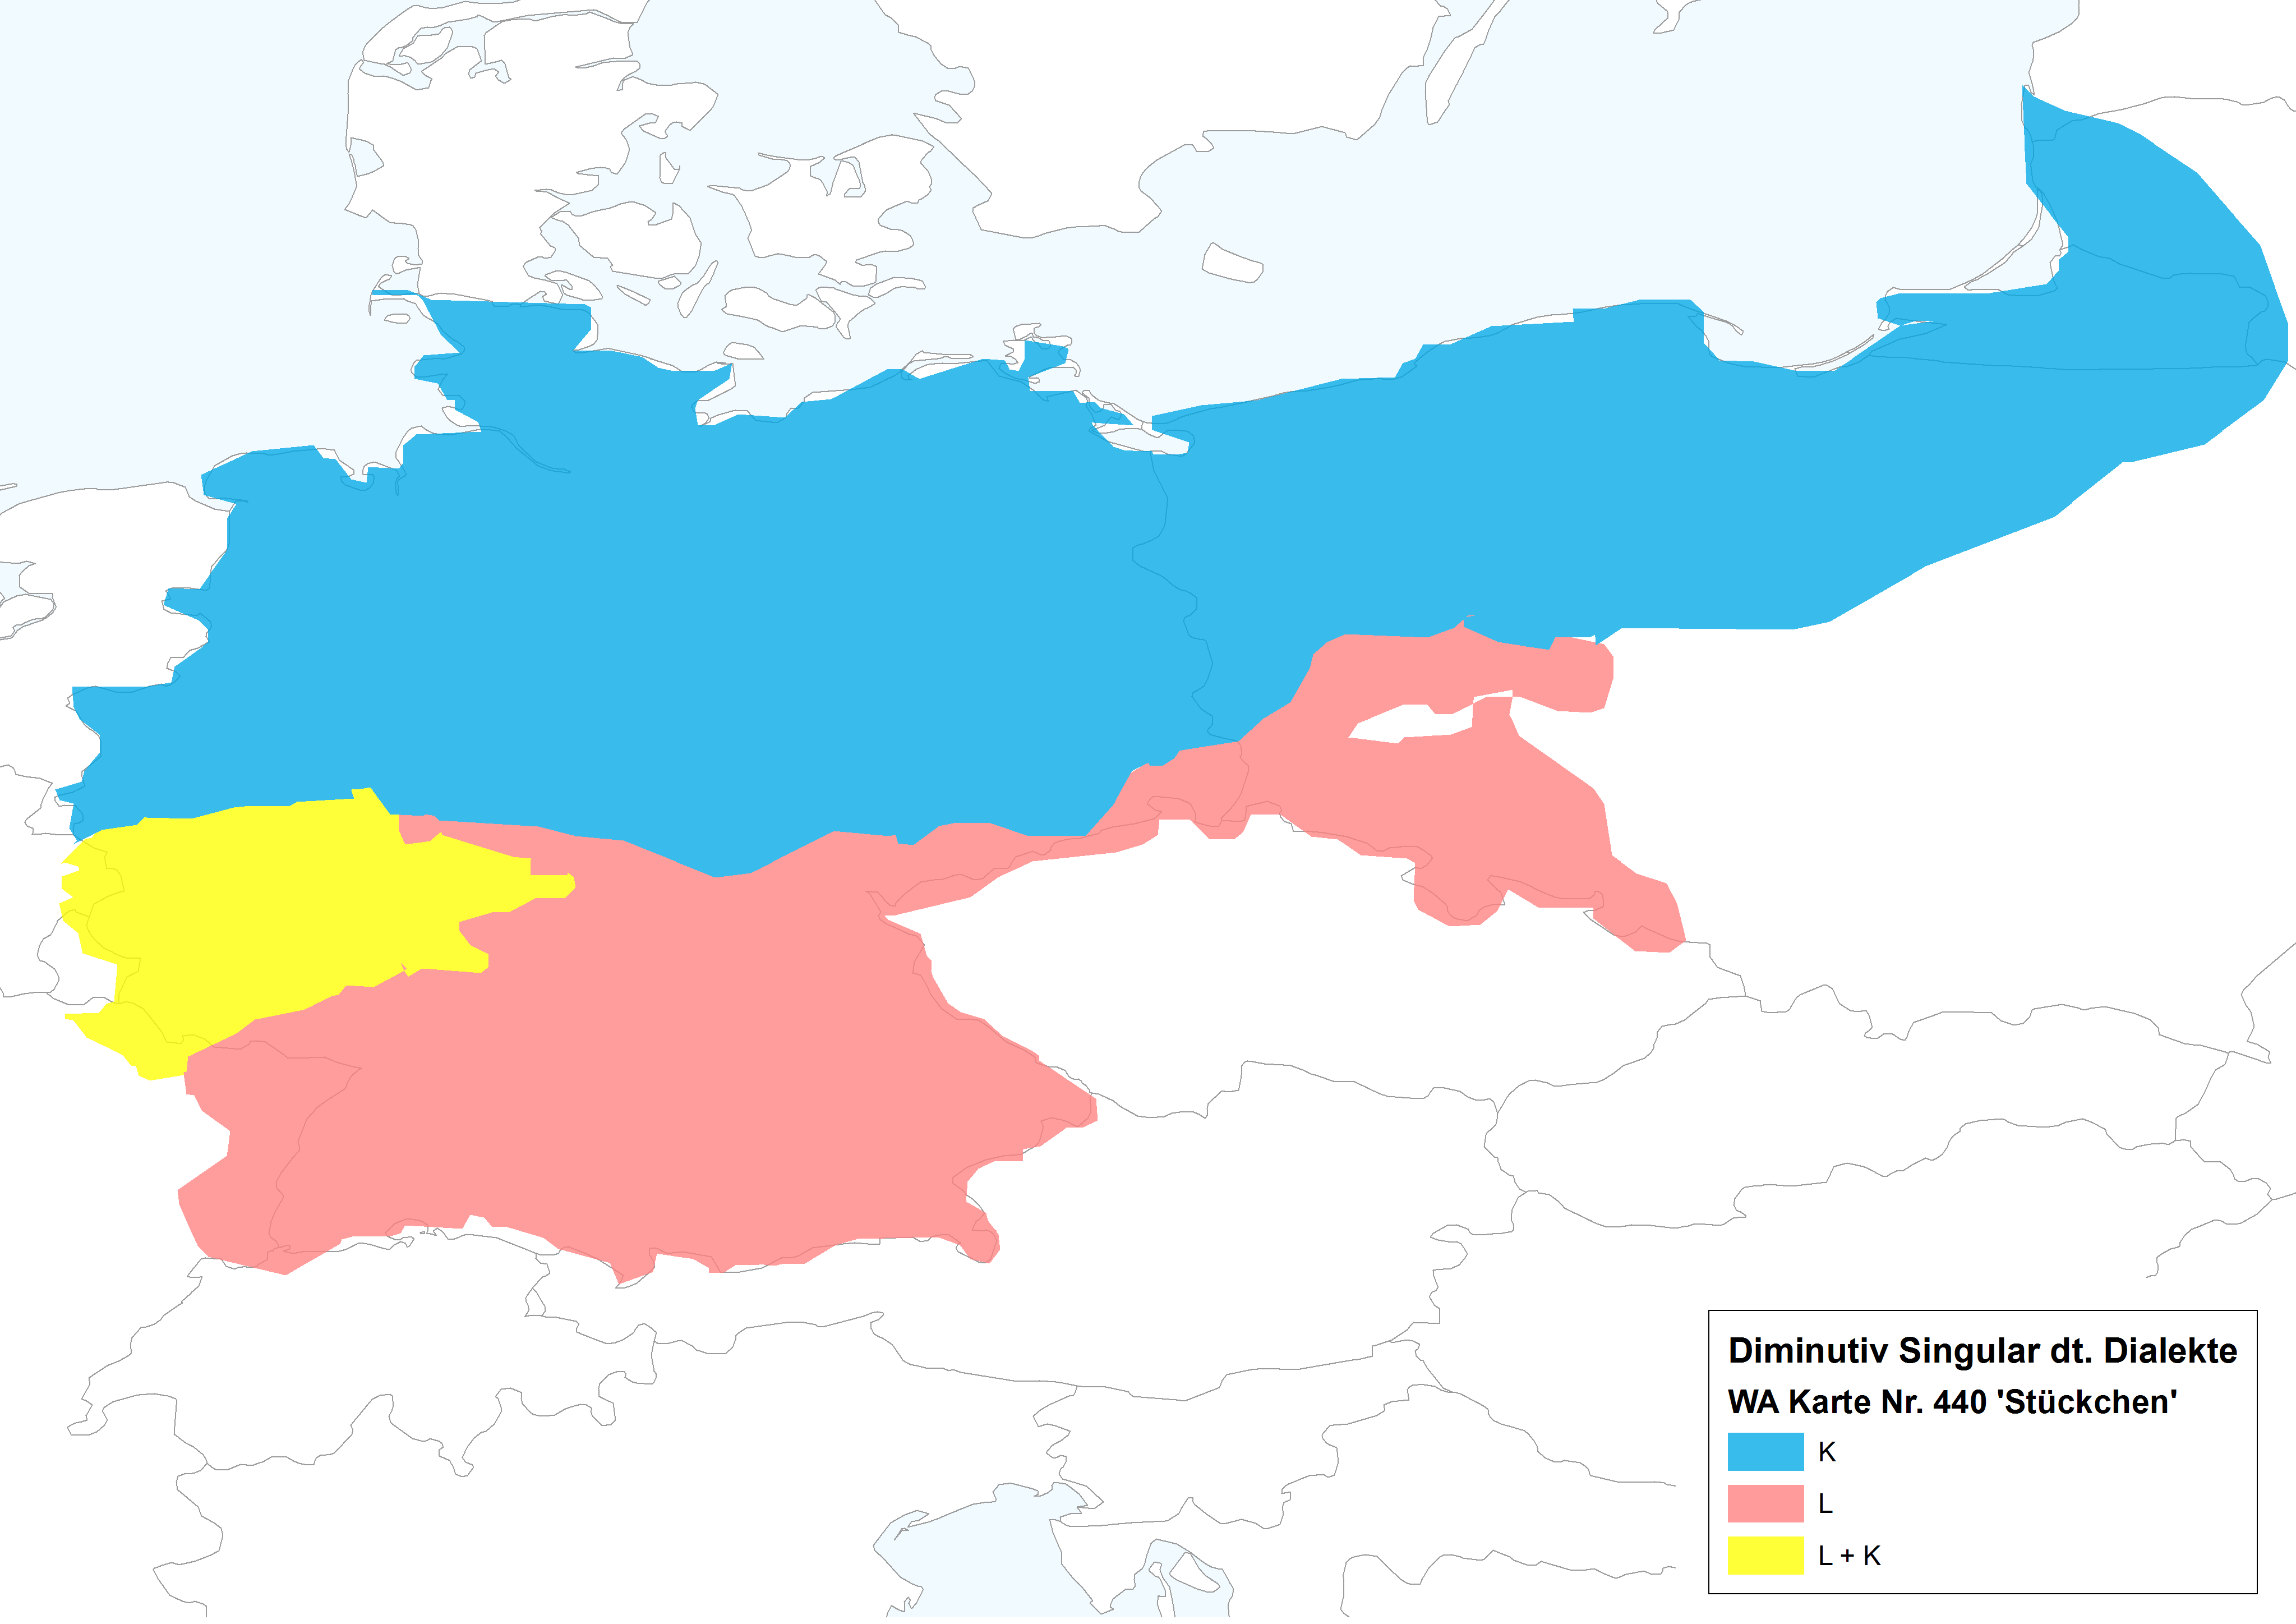
\includegraphics[scale=0.5]{figures/DSA_DIM_SG_kurz.png}
		\caption{\label{SgDimDSA} Singulardiminutionen in den dt. Dialekten (\hai{WA} Karte Nr. 440 \sem{Stückchen})}
		\end{figure}
\FloatBarrier 


	
		
		
		
  \begin{table}[h!]
%\begin{longtable}{ccc|ccc}
\centering
		\begin{tabular}{ll}

		\hline 

\textbf{Muster} &\textbf{Beispiel} (\sem{Ente\textsubscript{Dim. Pl.}})  \\ \hline 

\hai{K} & \textit{-che} \textit{Entche}, \textit{-ke} \textit{Entke} \\
\hai{L} & \textit{-le} \textit{Entla}, \textit{-ile} \textit{Entile} \\

\hai{L + K }& \textit{-lich} \textit{Entlich} \\
\hai{K + L }& \textit{-chel} \textit{Entchel} \\ 

\hai{Pl. + K }& \textit{-erche} \textit{Enterche}, \textit{-erje} \textit{Enterje} \\
\hai{Pl. + L }& \textit{-erle} \textit{Enterle}\\

\hai{K + Pl.} & \textit{-kes} \textit{Entkes}, \textit{-cher} \textit{Entcher} \\
\hai{L + Pl.} & \textit{-len} \textit{Entlen} \\


\hai{Pl. + K + Pl.} & \textit{-ercher} \textit{Entercher}, \textit{-erchens} \textit{Enterchens} \\

  \hline 
 \end{tabular}
		 \caption{Grundmuster von Pluraldiminutivsuffixen im Deutschen (basierend auf \hai{WA} Karte Nr. 381 \sem{Apfelbäumchen})}
		 \label{tblDIMsystem}
		 \end{table}
		% \end{longtable}
		
 

 \begin{figure}[h!]
\centering
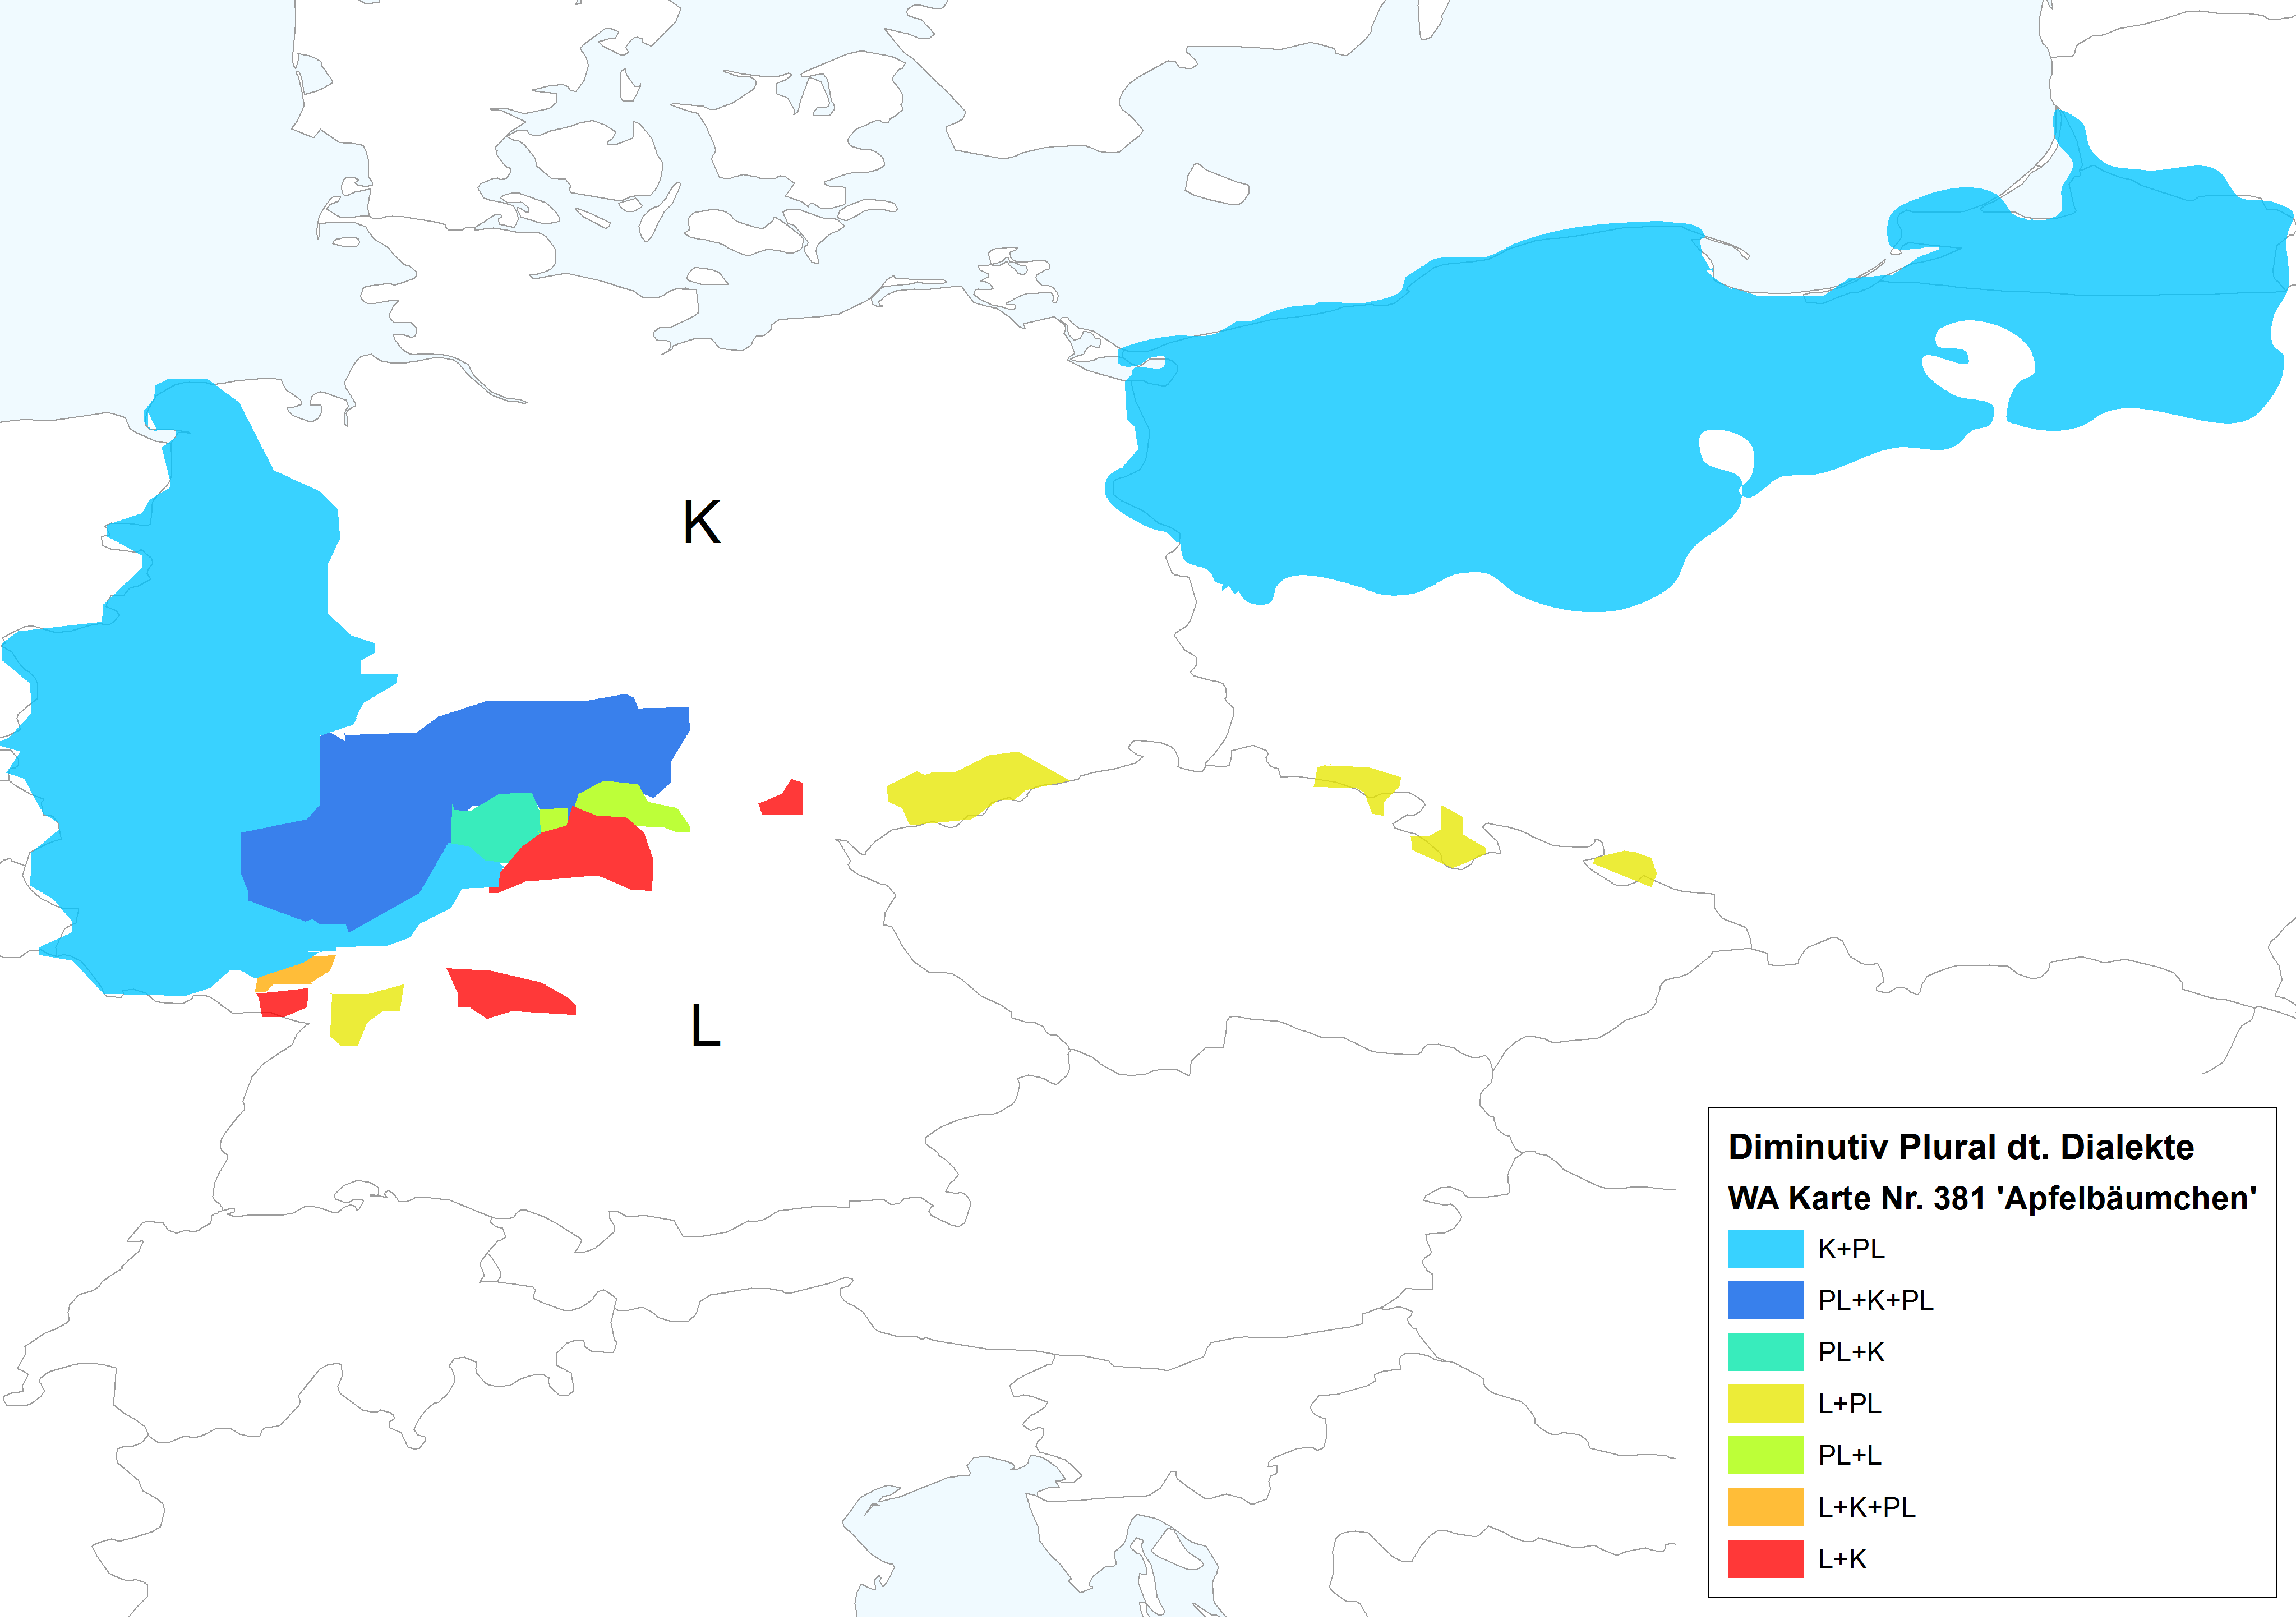
\includegraphics[scale=0.5]{figures/DSA_DIM_PL_kurz.png}
		\caption{\label{DimDSA} Pluraldiminutionen in den dt. Dialekten (\hai{WA} Karte Nr. 381 \sem{Apfelbäumchen})}
		\end{figure}
\FloatBarrier








\subsection{\isi{Diminution} im Jiddischen}\label{dimJIDDISCH}
%  %\noindent
Das Diminutionssystem des modernen Ostjiddischen fasst Tabelle  \ref{tblDIMOJ} zusammen. Der Singular wird mittels -\textit{l} (1. Grad) und -\textit{ele} (2. Grad)\footnote{Das Suffix -\textit{ele} findet sich auch bei auf /l/ auslautenden Nomina auch im 1. Grad, z.\,B. \RL{פֿויגל} \textit{foygl} \sem{Vogel} \RL{פֿייגעלע} \textit{feygele} \sem{Vogel\textsubscript{Dim. Sg.}}} gebildet (\cite[69]{Jacobs2005}; \cite[80]{Perlmutter1988}). Die Pluraldiminution wird mittels -\textit{lekh} (1. Grad) bzw. -\textit{elekh} (2. Grad) gebildet (\cite[162–163]{Jacobs2005}; \cite[80]{Perlmutter1988}). Bei Nomina mit \ili{hebräisch}-aramäischer Wurzel findet sich oftmals eine doppelte  Pluralmarkierung, indem \textit{-(e)lekh} an das bereits im Plural stehende Nomen gehängt wird, wie z.\,B. in \RL{חסיד} \textit{khsid} \sem{Frommer\textsubscript{Sg.}} > \RL{חסידים} \textit{khsidim} \sem{Fromme\textsubscript{Pl.}} > \RL{חסידיםלעך} \textit{khsidimlekh} \sem{Frommer\textsubscript{Pl.+ Dim. Pl.}} (\cite[163]{Jacobs2005}; \cite{Perlmutter1988}). Dieselbe Situation lässt sich aber auch in einzelnen Lexemen der germanischen Komponente finden, z.\,B. in \RL{קינדערלעך} \textit{kinderlekh} \sem{Kind\textsubscript{Pl. + Dim. Pl.}} (\cite[163]{Jacobs2005}; \cite{Perlmutter1988}). Jiddisch orientiert sich damit an der \hai{L}-\isi{Diminution}, die im Ober- und Mitteldeutschen verbreitet ist. Das \isi{Pluralsuffix} findet sich in den deutschen Dialekten des Ost- und Rheinfränkischen als -\textit{lich} belegt, wo es sich entlang der Isoglosse zwischen \hai{L}- und \hai{K}-\isi{Diminution} als Fusionsform beider Formen herausgebildet hat (\cite[647]{Grimm1890}; \cite[245]{Weinhold1867}; \cite[124]{Wrede1908}; \cite[49]{Paul1920}).\footnote{Die Analyse des Suffixes als Fusion der zwei Basistypen von \isi{Diminution} wird nicht von jedem geteilt. Z.\,T. wird dieses Suffix als \isi{Komposition} von \hai{L}-\isi{Diminution} und dem Kollektivsuffix ahd. -\textit{ahi}, mhd. -\textit{ech} (-\textit{ach}, -\textit{ich}), nhd. -\textit{icht} (un\isi{produktiv} z.\,B. in \textit{Kehricht}, \textit{Dickicht}) analysiert, so etwa in \textcite[484]{Schirmunski1962}, \textcite[110–112]{Timm2005}. \textcite[235]{Weinhold1867} schlägt vor, dass die Existenz des Kollektivsuffixes als Katalysator für die Grammatikalisierung der Fusionsform als \isi{Pluralsuffix} gewirkt haben mag. Ebenso können auch die -\textit{ach}-Plurale des Oberdeutschen dazu beigetragen, der Fusionsform -\textit{lich} Pluralbedeutung zu geben (vgl. \cite{Rowley1994}).}\\ 



 \begin{table}[h!]
%\begin{longtable}{ccc|ccc}
\centering
		\begin{tabular}{llll}

		\hline 

\textbf{Grad} &\textbf{Numerus} & \textbf{Suffix} & \textbf{Beispiel \sem{Lied}} \\ \hline 

1. & Sg. & -\textit{l} & \RL{לידל} \textit{lidl} \sem{kleiner Lied} \\

1. & Pl. & -\textit{lekh} & \RL{לידלעך} \textit{lidlekh} \sem{kleine Lieder} \\ \hdashline

2. & Sg. & -\textit{ele} &  \RL{לידעלע} \textit{lidele} \sem{zärtlich \textit{Lied}} \\ 

2. & Pl. & -\textit{elekh} &\RL{לידעלעך} \textit{lidelekh} \sem{zärtlich \textit{Lieder}} \\
 
 
 
  \hline 
 \end{tabular}
		 \caption{Das Diminutionssystem des standardisierten Ostjiddischen}
		 \label{tblDIMOJ}
		 \end{table}
		% \end{longtable}

Die Situation der \isi{Diminution} in den jiddischen Dialekten ist bislang noch nicht beschrieben worden. Die Daten des \hai{LCAAJ} (\citeyear[120]{Herzog2000}) lassen vermuten, dass es tatsächlich diatopisch unterschiedliche Suffixe gab und womöglich auch das System der graduellen Diminuierung de facto nicht soweit verbreitet war, wie das standardisierte Jiddisch vermuten lässt.\footnote{Die Daten zur \isi{Diminution} des \hai{LCAAJ} (\citeyear[120–125, insbes. Karte 36]{Herzog2000}) bieten nur einen minimalen Ausschnitt in die tatsächliche Sprachsituation. Dies zeigt sich besonders daran, dass hier im Singular zwei unterschiedliche und nicht miteinander vergleichbare Suffixe (\RL{שיקסע} \textit{shikse} \sem{Nichtjüdin} im Westjiddischen und \RL{מויל} \textit{moyl} \sem{Mund} im Ostjiddischen) die Basis bilden. Wie \textcite{Wrede1908} zeigt, ist die Wahl eines Diminutivsuffixes stark lexemgebunden, vgl. S. \pageref{wredeDIM}. Hinzu kommt, dass die Erhebungsmethode des Fragebogens im Westjiddischen kaum dazu ausreichte,  semantische Feinheiten wie die \isi{Diminution} 1. und 2. Grades einzufangen.} Dialektale Abweichungen vom Standard finden sich zum Beispiel im \hai{NOJ}, wo die Singulardiminuierung von  \RL{מויל} \textit{moyl} \sem{Mund}  mittels -\textit{kh(e)le} erfolgt, und im \hai{SOJ} findet sich das Suffix -\textit{lche(n)} im Lexem \RL{שיקסע} \textit{shikse} \sem{Nichtjüdin} (\cite[122, Karten 36S1, 36S2]{Herzog2000}). Wie in den deutschen Dialekten herrscht so scheinbar auch in den jiddischen Varietäten eine vom Lexem abhängige Vielfalt an Diminutivsuffixen vor (vgl. S. \pageref{wredeDIM}). Vor allem aber fällt die Datenmenge des \hai{LCAAJ} zu gering aus, als dass sich auf deren Basis Aussagen über das jiddische Diminutionssystem machen ließen.\label{SOJDIM}

Dies zeigt sich besonders im Westjiddischen. Den Daten des \hai{LCAAJ} (\citeyear[120–125]{Herzog2000}) zufolge bildet das Westjiddische die Singulardiminution im \hai{SWJ} und südwestlichen \hai{ZWJ} mittels -\textit{(e)le}, im \hai{NWJ} und \hai{NÜJ} mittels -\textit{l}, im \hai{SÜJ} finden sich beide Suffixe parallel und im westlichen \hai{ZWJ} ist -\textit{che(n)} zu finden (\cite[120–122, Karten Nr. 36, Nr. 36S1]{Herzog2000}). \citeauthor{GuggenheimGruenberg1973}s Daten zum südlichen \hai{SWJ} und \hai{ZWJ} bestätigen dieses Bild nicht; vielmehr finden sich hier die den koterritorialen deutschen Dialekten entsprechenden Suffixe (\cite[92, Karte Nr. 33]{GuggenheimGruenberg1973}). Dieses Bild bestätigen auch schriftliche Quellen aus dem 19. und 20. Jahrhundert. So findet sich im Westjiddischen nördlich des Mains die \hai{K}-\isi{Diminution} (Bsp. \ref{BspSGWJ1}–\ref{BspSGWJ3}) und im Süden \hai{L}-\isi{Diminution} (Bsp. \ref{BspSGWJ4}–\ref{BspSGWJ6}).\\ \label{DIMSGWJ}

 \eenumsentence{
 
 \item \textit{Stickche} \sem{Stück\textsubscript{Dim. Sg.}}  \\
 \textit{Schnüpfche} \sem{Schnupfen\textsubscript{Dim. Sg.}} \\
(\qu{Das verfrühte Schulenrufen} Aurich 1902 [\cite[67]{Reershemius2007}])  \label{BspSGWJ1}


  \item \textit{Goichen} \sem{Nichtjude\textsubscript{Dim. Sg.}} \\
  (\qu{Die Lebenserinnerungen des A. H. Heymann}, Strausberg (Berlin), 1909:\,92 [\cite[39]{Schaefer2010}])  \label{BspSGWJ2}


 \item \RL{תמרכה} \textit{tamarche} \sem{Tamara\textsubscript{Dim. Sg.}} \\
 \RL{גומפלכה}  \textit{gumplche} \sem{Gumpel\textsubscript{Dim. Sg.}} \\
 (\qu{Die Hochzeit zu Grobsdorf} 1822:\,dramatis personae) \label{BspSGWJ3}
 
  
   \item \textit{Großvaterle} \sem{Großvater\textsubscript{Dim. Sg.}}  \\
   (\qu{Die Juden von Zirndorf} Fürth, 1897 [1996]:\,177)\label{BspSGWJ4}
   
    \item \textit{Stickle} \sem{Stück\textsubscript{Dim. Sg.}}  \\
    \textit{Peckle} \sem{Packet\textsubscript{Dim. Sg.}}  \\
      (\qu{Garkisch} Mulhouse, 1930:\, 9; 20) \label{BspSGWJ5}
      
            
    \item \textit{Stickl} \sem{Stück\textsubscript{Dim. Sg.}}  \\
     \textit{Majerl} \sem{Mauer\textsubscript{Dim. Sg.}}  \\
 (Wenkerbogen aus Frauenkirchen Nr. 42663/300447; vgl. \cite{FleischerSchaeferErsch}) \label{BspSGWJ6}
 
 }

Der \hai{LCAAJ} erweckt mit der einzigen Kartierung eines durchaus problematischen\footnote{Problematisch an diesem Lexem als Stellvertreter der Pluraldiminution ist, dass die \isi{Diminution} bereits erstarrt sprich lexikalisiert, sein könnte. Vgl. dazu auch den westjiddischen Beleg in Bsp. \ref{bspDIMPLlichAURICH} S. \pageref{bspDIMPLlichAURICH} (\cite[133]{Reershemius2007}).} Lexems mit Pluraldiminution \RL{קרעפלעך} \textit{kreplekh} \sem{Knödel\textsubscript{Dim. Pl.}} den falschen Eindruck, dass das Westjiddische über keine vom Singular distinkte Pluraldiminution wie das Ostjiddische verfügt. Der westlichste Beleg für die \isi{Diminution} mittels -\textit{lekh} im \hai{LCAAJ} findet sich in Prag. Dies ist ein besonders eindrucksvolles Beispiel für die Unzulänglichkeit der westjiddischen Daten des \hai{LCAAJ}, denn selbst \textcite[94, Karte Nr. 34]{GuggenheimGruenberg1973} gelingt es, die westjiddische Pluraldiminution mittels -\textit{lich} einzufangen. \textcite[56]{Zuckerman1969}, dessen Daten eigentlich in die Kartierung des \hai{LCAAJ} hätten einfließen müssen, findet dieses Suffix im Elsässer Jiddisch. Die ersten Belege für Pluraldiminutivbildungen auf -\textit{lich} sind aus dem Mitteljiddischen, d.\,h. aus dem 15. bis 17. Jahrhundert, bekannt (\cite[112]{Timm2005}). Das historische Diminutivsystem des Jiddischen zeigt noch generell eine hohe Vielfalt der Suffixe (\cite[109–113]{Timm2005}). Damit ist anzunehmen, dass das moderne System, wie es Tabelle \ref{tblDIMOJ} zeigt, tatsächlich eine Idealisierung eines wahrscheinlich wesentlich komplexeren Systems darstellt. Tatsächlich lässt sich im Fall der Pluraldiminution ein Ost-West-Gefälle innerhalb des jiddischen Dialektgebiets erkennen: Aus dem Westjiddischen sind uns bislang lediglich Quellen mit dem Suffix -\textit{lich}/-\textit{lisch} (Bsp. \ref{bspDIMPLlich}–\ref{bspDIMPLlisch}) überliefert, im \hai{NÜJ} findet sich vereinzelt das Suffix -\textit{lech} (Bsp. \ref{bspDIMPLlechHeymann}–\ref{bspDIMPLlech}) und im \hai{SÜJ} und südwestjiddischen Randgebieten zum \hai{SÜJ} -\textit{loch} und -\textit{lach} (Bsp. \ref{bspDIMPLloch}–\ref{bspDIMPLlach}). Allem Anschein nach ist also die Wahl des Vokals eine regional variierende Komponente. Hinzu kommt, dass im Westjiddischen nördlich des Mains das sonst für das Jiddische übliche \isi{Pluralsuffix} -\textit{l}- +  Vokal + -\textit{ch} nur in zwei umstrittenen Belegen vorliegt.\footnote{Diese beiden Belege sind in den Bsp. \ref{bspDIMPLlichAURICH} u. \ref{bspDIMPLlechHeymann} angeführt. Der Beleg aus Aurich kann, wie \textcite[133 Fn. 199]{Reershemius2007} anführt, als ostjiddisches \isi{Lehnwort} im Diminutiv Plural erstarrt sein. Ebenfalls ein ostjiddischer Einfluss ist im Beleg aus Strausberg möglich, da auch dieses Lexem nicht im Westjiddischen belegt ist, vgl. \textcite[40f]{Schaefer2010}. Die Wahl des Vokals im Diminutivsuffix spricht jedoch in beiden Fällen dafür, dass hier eine regionale Form vorliegt und nicht eine aus dem Ostjiddischen entlehnte.} Das allgemeine Bild westjiddischer (Plural-)\isi{Diminution} im Norden des Sprachgebiets scheint eine größere Variation zu haben, als es im Südwesten der Fall ist. Ein eindrucksvolles und glaubwürdiges Beispiel ist hier \qu{Die Hochzeit zu Grobsdorf}, in der eine hohe Varianz an Diminutivsuffixen im Plural\footnote{Im Singular findet sich hier regulär \RL{כה}- \textit{-che}. Die Pluralsuffixe, wie auch das Singularsuffix, können selbstverständlich aus dem Kontakt zu den koterritorialen hessischen Dialekten ins örtliche Jiddisch Eingang gefunden haben, da dort eben solche Suffixe gebräuchlich sind, vgl. \hai{WA} Karten Nr. 381, 440; \textcite[86]{Friebertshaeuser1987}.} vorliegt (Bsp. \ref{bspDIMPLgrob}). Wichtig ist festzuhalten, dass kein im Jiddischen vorkommendes Suffix nicht auch in einem deutschen Dialekt belegt ist.\footnote{Es besteht selbstverständlich die generelle Möglichkeit, dass im Ostjiddischen \isi{Diminution} auch mittels slawischer Suffixe (insbes. -\textit{ke}) gebildet werden können. Eine umfassende Untersuchung zum ostjiddischen Diminuierungssystem müsste diesen Fall zumindest berücksichtigen, da das Suffix selbst (wenn auch un\isi{produktiv}) in vielen Lexemen der slawischen  Komponente vorhanden ist, z.\,B. \RL{קא\makebox(-1.5,-7.5)[r]{\libertineGlyph{uni207B}}טשקע} \textit{katshke} \sem{Ente} (vgl. poln. \textit{kaczka} \sem{Ente}), \RL{מא\makebox(-1.5,-7.5)[r]{\libertineGlyph{uni207B}}רגעריטקע} \textit{margeritke} \sem{Gänseblümchen} (vgl. poln. \textit{margerytka} \sem{Gänseblümchen}).}\\

 \eenumsentence{

\item \RL{מא\makebox(-1.5,-7.5)[r]{\libertineGlyph{uni207B}}דליך} \textit{madlich} \sem{Mädchen\textsubscript{Dim. Pl.}} \\
\RL{הורג-ליך} \textit{horeg-lich} \sem{Zwerg\textsubscript{Dim. Pl.}}\\
(\qu{Esther. Oder die belohnte Tugend} Fürth, 1854:\, 7; 17) \label{bspDIMPLlich} 

\item \textit{Kneidlich} \sem{Knödel\textsubscript{Dim. Pl.}} \\
(\qu{Das verfrühte Schulenrufen} Aurich 1902:\,3. Auftritt [\cite[133]{Reershemius2007}]) \label{bspDIMPLlichAURICH}

 \item \textit{Blimlisch} \sem{Blumen\textsubscript{Dim. Pl.}}\\
  \textit{Sticklisch} \sem{Stücke\textsubscript{Dim. Pl.}} \\
  (\qu{Garkisch} Mulhouse, 1930:\, 15; 16) \label{bspDIMPLlisch}
 
 \item \textit{Rendlech} \sem{Münze\textsubscript{Dim. Pl.}} \\
 (\qu{Die Lebenserinnerungen des A. H. Heymann}, Strausberg (Berlin), 1909:\,5  [\cite[40]{Schaefer2010}])  \label{bspDIMPLlechHeymann}
 
 \item \textit{Bäumlēch} \sem{Baum\textsubscript{Dim. Pl.}} \\
  \textit{Äpelech} \sem{Apfel\textsubscript{Dim. Pl.}} \\
 (Wenkerbogen aus Kobyla Góra Nr. 09746; vgl. \cite{FleischerSchaeferErsch}) \label{bspDIMPLlech}
 
 \item \textit{Schefeloch} \sem{Schaf\textsubscript{Dim. Pl.}}\\
  \textit{Eppeloch} \sem{Apfel\textsubscript{Dim. Pl.}} \\
 (Wenkerbogen aus Frauenkirchen Nr. 42663/300447; vgl. \cite{FleischerSchaeferErsch}) \label{bspDIMPLloch}

 \item \textit{Kinderlach}  \sem{Kind\textsubscript{Dim. Pl.}}\\
  \textit{Bondlach}  \sem{Bund\textsubscript{Dim. Pl.}}\\
(\qu{Torres Lokschen} Budapest, 1900:\, 39, 49; 40) \label{bspDIMPLlach}

 \item \RL{מערערכער} \textit{merercher} \sem{Mädchen\textsubscript{Dim. Pl.}} \\
 (\qu{Die Hochzeit zu Grobsdorf} 1822:\,14, 110)\\
 \RL{קערלכה} \textit{kerlche} \sem{Kerl\textsubscript{Dim. Pl.}}\\
 (\qu{Die Hochzeit zu Grobsdorf} 1822:\,37) \label{bspDIMPLgrob} 
 
 }


 
  \subsection{\isi{Diminution} im \hai{chrLiJi1}}\label{dimsg}
  %  %\noindent
 
Wie eingangs erwähnt (S. \pageref{AnzahlDIM}) liegt im \hai{chrLiJi1} eine Vielzahl an Suffixen zur Singulardiminution vor, die im einzelnen mit Beispielbelegen versehen in Tabelle \ref{tblDIMSG} angeführt sind. An erster Stelle steht das Suffix -\textit{che(n)}, wie es auch in der deutschen Schriftsprache Verwendung findet. In diesen Fällen erfolgt also die Markierung der jüdischen Figuren weniger über die Abweichung von der schriftsprachlichen Norm, als durch eine auffallend häufige Verwendung der \isi{Diminution}.\footnote{Um gesicherte Aussagen über die \isi{Frequenz} von Diminutiva im Text jüdischer Figurenrede im Vergleich zu nicht-jüdischer Figuren zu machen, reichen die hier erhobenen Daten selbstverständlich nicht aus. Die Feststellung, dass \isi{Diminution} im Text  jüdischer Figuren die übliche \isi{Frequenz} von \isi{Diminution} übersteigt, beruht hier lediglich auf der Leseerfahrung der Verfasserin.} In zwölf Quellen und damit zweithäufigstes Suffix ist -\textit{el}. Dieses Suffix tritt in den deutschen Dialekten in kleinen Teilen des Niederalemannischen, Rheinfränkischen, Obersächsischen und Schlesischen auf (\hai{WA} Karte Nr. 440) und entspricht der ostjiddischen Singulardiminution des 1. Grads (s. Tabelle \ref{tblDIMOJ}, S. \pageref{tblDIMOJ}). Das Suffix -\textit{ele}, welches den 2. Grad der Singulardiminution im Ostjiddischen bildet, findet sich in nur zwei Quellen des \hai{chrLiJi1}. Mit einer Belegzahl von zehn Quellen ebenfalls sehr häufig ist die Fusionsform -\textit{elche(n)}. Diese ist in hessischen, rhein- und moselfränkischen Dialekten weit verbreitet (\hai{WA} Karte Nr. 440). 

Die Darstellung der Einzelformen in Abb. \ref{SgDimliji} zeigt, dass einzelne Suffixe in bestimmten Gebieten besonders häufig auftreten. So etwa das Suffix \textit{-el}, welches neben zwei Belegen aus Bonn, vor allem im Nordosten und im Südosten und damit in Kontaktzonen zum Ostjiddischen zu finden ist. Es könnte sich dabei um eine \isi{Emulation} des ostjiddischen Singularsuffix des 2. Diminutionsgrades \textit{-ele} handeln. Ebenfalls räumlich auffällig verhalten sich die Belege des Suffix \textit{-elche(n)}, welches wir zwar besonders im westmitteldeutschen Raum finden, wo es auch in den deutschen Dialekten verbreitet ist (vgl. Karte in Abb. \ref{SgDimDSAliji}), allerdings ist es auch im Nordosten vielfach belegt, wo es für die deutschen Dialekte untypisch ist. 


Vier Quellen zeigen das Pluraldiminutivsuffix -\textit{lich} im Singular (s. Abb. \ref{DimDSALiJilich}, S. \pageref{DimDSALiJilich}). Eine solche Verwendung dieses Suffixes im Singular ist weder aus jiddischen noch aus deutschen Varietäten bekannt. Da all diese Quellen das Suffix auch \quein{korrekt} bei der \isi{Diminution} Plural einsetzen, ist anzunehmen, dass es sich hierbei um Hyperkorrekturen handelt.\label{lichHyper} Den meisten Autoren des \hai{chrLiJi1} mag also nicht bewusst gewesen sein, dass das Jiddische eine Unterscheidung zwischen Diminutiv Singular und Plural trifft, und so wurde das  \isi{Pluralsuffix} auf den Singular übertragen.\footnote{Hinzukommt, dass mindestens ein Text durch die Schriften Itzig Veitel Sterns (pseud.) (\hai{GP}  Nürnberg, 1831) beeinflusst ist, welcher -\textit{lich} sowohl im Singular als auch im Plural verwendet; zumindest nennt der Verfasser von \hai{PG} (Speyer, 1835) im Vorwort diesen als sein Vorbild (vgl. Abschnitt \ref{IVS}, S. \pageref{IVS}).} 

Die Kartierung der Daten in den Abbildungen \ref{SgDimliji} und \ref{SgDimDSAliji} zeigt, dass \hai{L}-\isi{Diminution} über das gesamte Erhebungsgebiet verteilt vorliegt, während \hai{K}-Diminutionen im Süden rar sind. Davon ausgehend lässt sich vermuten, dass einigen der Autoren bewusst war, dass die \isi{Diminution} im Jiddischen auf den \hai{L}-Typ aufbaut. Interessant ist außerdem, dass Fusionsformen nach dem Muster \hai{L+K} im gesamten Gebiet (mit Ausnahme des äußersten Südostens) belegt sind, obwohl diese Form eigentlich charakteristisch für die westmitteldeutschen Dialekte ist. Die bislang bekannten Daten zum Westjiddischen sprechen nicht dafür, dass im Singular solche Fusionsformen dort weit verbreitet waren (vgl. S. \pageref{DIMSGWJ}). Da jedoch generell die Datengrundlage recht dünn ist, was auch dem Umstand geschuldet ist, dass \isi{Diminution} außerhalb des \hai{LiJi} kein besonders frequentes Phänomen ist und die Wahl der einzelnen Suffixe von Wort zu Wort variieren kann, lässt sich nicht mit Bestimmtheit ausschließen, dass das \hai{chrLiJi1} hier eventuell etwas einfängt, was in den authentischen Quellen des Westjiddischen nicht belegt ist, tatsächlich aber Teil der Sprachrealität war. Für die Existenz einer Fusionsform der Singulardiminutionssuffixe im Jiddischen spricht, dass solche Formen auch im Ostjiddischen belegt sind (\cite[122, Karten 36S1, 36S2]{Herzog2000}; vgl. S. \pageref{SOJDIM}) und dass ich das Pluraldiminutivsuffix -\textit{lich}/ -\textit{lekh} als aus einer \hai{L}-\hai{K}-Fusion hervorgegangen auffassen.


Die Karten in Abb. \ref{SgDimliji} und \ref{SgDimDSAliji} ließen die Vermutung zu, dass \hai{L}-Diminutionen durch ostjiddischen Einfluss erst im Verlauf des 19. Jahrhunderts im Norden auftauchen. Das Histogramm in Abb. \ref{REGDIMSG}, welches die Quellen je nach regionaler Lage im deutschen Diminutionssystem (ausgehend von \hai{WA} Karte Nr. 440) sortiert, zeigt aber, dass wir in der \hai{K}-Region, also im Norden des Untersuchungsgebiets, bereits um 1800 \hai{L}-\isi{Diminution} vorfinden. Ebenso ist \hai{K}-\isi{Diminution} in den älteren Quellen im Süden (\hai{L}-Region) belegt.\label{LKinberlin} Die Fusionsformen \hai{L+K} hingegen zeigen insofern ein areales Muster, als dass wir sie nur in zwei relativ jungen Quellen in der \hai{L}-Region finden, und sie besonders im Norden (\hai{K}-Region) frequent sind. Eine diachrone Entwicklung von Diminutivtypen im \hai{chrLiJi1} ist also nicht festzustellen. Generell zeigen Karten und Diagramm deutlich, dass im Norden (\hai{K}-Region) mehr von der regionalen Variante (in dem Fall auch der schriftsprachlichen Variante) abweichende Variation zu finden ist, als in der (westlichen) Mitte (\hai{L+K}-Region) oder im Süden (\hai{L}-Region). Zu beachten ist, dass sich die meisten Belege der \hai{K}-\isi{Diminution} aus dem schriftsprachlichen Suffix \textit{-chen} ergeben (wenn auch in manchen Fällen mit gesprochensprachlichem \textit{n}-Ausfall) und damit eher als Hintergrundrauschen der Schriftsprache denn als tatsächliche Evidenz für eine literaturjiddische Manipulation zu deuten sind.\footnote{Es wurde darauf verzichtet, ein vergleichbares Diagramm wie jenes in Abb. \ref{REGDIMSG} für die Pluraldiminution mit anzuführen, da dieses ebenfalls keine Beziehungen zwischen zeitlich-räumlichen Auftreten einer Struktur im \hai{chrLiJi1} aufweist.}\label{sgDIMimNordenmehr} Ebenfalls als Reflex der deutschen Schriftsprache sind Belege für das Suffix \textit{-ge} zu deuten, da dieses Suffix noch bis ins 18. Jahrhundert als \qu{Leitvariante} der \isi{Diminution} galt und im 19. Jahrhundert, wenn auch sukzessive durch \textit{-chen} abgelöst, noch immer gebräuchlich ist (\cite{Wegera2000b}; \cite[73f]{Elspass2005}).\\


  \begin{table}[h!]
%\begin{longtable}{ccc|ccc}
%\centering
		\begin{tabularx}{\columnwidth}{lXc}

		\hline 

\textbf{Suffix} &\textbf{Beispiel} & \textbf{Quellen} \\ \hline 


\textit{-che(n)} & \textit{Doktor-Titelche} \sem{Doktortitel\textsubscript{Dim. Sg.}} (\hai{PG}:\,3), \textit{Doktorche} \sem{Doktor\textsubscript{Dim. Sg.}} (\hai{JK}:\,4, 5, 8), \textit{Pferdchen} \sem{Pferd\textsubscript{Dim. Sg.}} (\hai{JP}:\,5) & 28 \\ 

 
 \textit{-ge} & \textit{Biksge} \sem{Büchse\textsubscript{Dim. Sg.}} (\hai{PA}:\,9),  \textit{Stückge} \sem{Stück\textsubscript{Dim. Sg.}} (\hai{PA}:\,34) & 1 \\ %\textit{bisge } \sem{bisschen\textsubscript{Dim. Sg.}} (\hai{PA}:\,73) 
 
 \textit{-je} & \textit{Musje } \sem{Maus\textsubscript{Dim. Sg.}} (\hai{PP}:\,30) & 1\\

 \textit{-ke} & \textit{Britschke } \sem{Pritsche\textsubscript{Dim. Sg.}} (\hai{AJ}:\,6),  \textit{Marieken} \sem{Marie \textsubscript{Dim. Sg.}} (\hai{DP}:\,27) & 2 \\
 
 \textit{-elche(n)} & \textit{Wechselche } \sem{Wechsel\textsubscript{Dim. Sg.}} (\hai{PA}:\,11),  \textit{Ringelche } \sem{Ring \textsubscript{Dim. Sg.}} (\hai{WA}:\,165),  \textit{Ringelchen } \sem{ Ring\textsubscript{Dim. Sg.}} (\hai{FS}:\,44) & 10 \\
 

 \textit{-elgen} & \textit{Mägelgen} \sem{Magen\textsubscript{Dim. Sg.}} (\hai{OF}:\,1) & 1 \\
 
 \textit{-lach} & \textit{Stickelach} \sem{Stück\textsubscript{Dim. Sg.}} (\hai{SS}:\,10) &1 \\
 
 \textit{-lich} & \textit{Hütlich} \sem{Hut\textsubscript{Dim. Sg.}} (\hai{SV}:\,3),  \textit{Hälslich} \sem{Hals\textsubscript{Dim. Sg.}} (\hai{LM}:\,22),  \textit{Sußlich} \sem{Pferd\textsubscript{Dim. Sg.}} (\hai{GP} Nürnberg, 1831:\,35, 36), \textit{Lämmlich} \sem{Lamm} (\hai{PG}:\,11) & 4\\
 
 \textit{-lein} & \textit{Stücklein } \sem{Stück\textsubscript{Dim. Sg.}} (\hai{HJ}:\,101),  \textit{Büchlein} \sem{ Buch\textsubscript{Dim. Sg.}} (\hai{LM}:\,12) & 2\\
 
 \textit{-le} & \textit{Bäuerle } \sem{Bauer\textsubscript{Dim. Sg.}} (\hai{PA}:\,)VIII,  \textit{Davidle} \sem{ David\textsubscript{Dim. Sg.}} (\hai{OF}:\,2),  \textit{Schwesterle } \sem{ Schwester\textsubscript{Dim. Sg.}} (\hai{AK}:\,247) & 7\\
 
 \textit{-el} & \textit{Bauernmädel} \sem{Bauernmädchen\textsubscript{Dim. Sg.}} (\hai{PP}:\,21),  \textit{Päckel} \sem{Packet\textsubscript{Dim. Sg.}} (\hai{FE}:\,56),  \textit{Schicksel} \sem{Nichtjüdin\textsubscript{Dim. Sg.}} (\hai{JP}:\,5) & 12\\

 \textit{-ele} & \textit{Mouschele} \sem{Mose\textsubscript{Dim. Sg.}} (\hai{OF}:\,2),  \textit{Patschhäntele} \sem{Patschehand \textsubscript{Dim. Sg.}} (\hai{GW}:\,13) & 2\\
 
 \hline 
 \end{tabularx}
		 \caption{Diminutivsuffixe Singular im \hai{chrLiJi1}}
		 \label{tblDIMSG}
		 \end{table}
		% \end{longtable}

 
  
 \FloatBarrier
 
 
   \begin{figure}[h!]
\centering
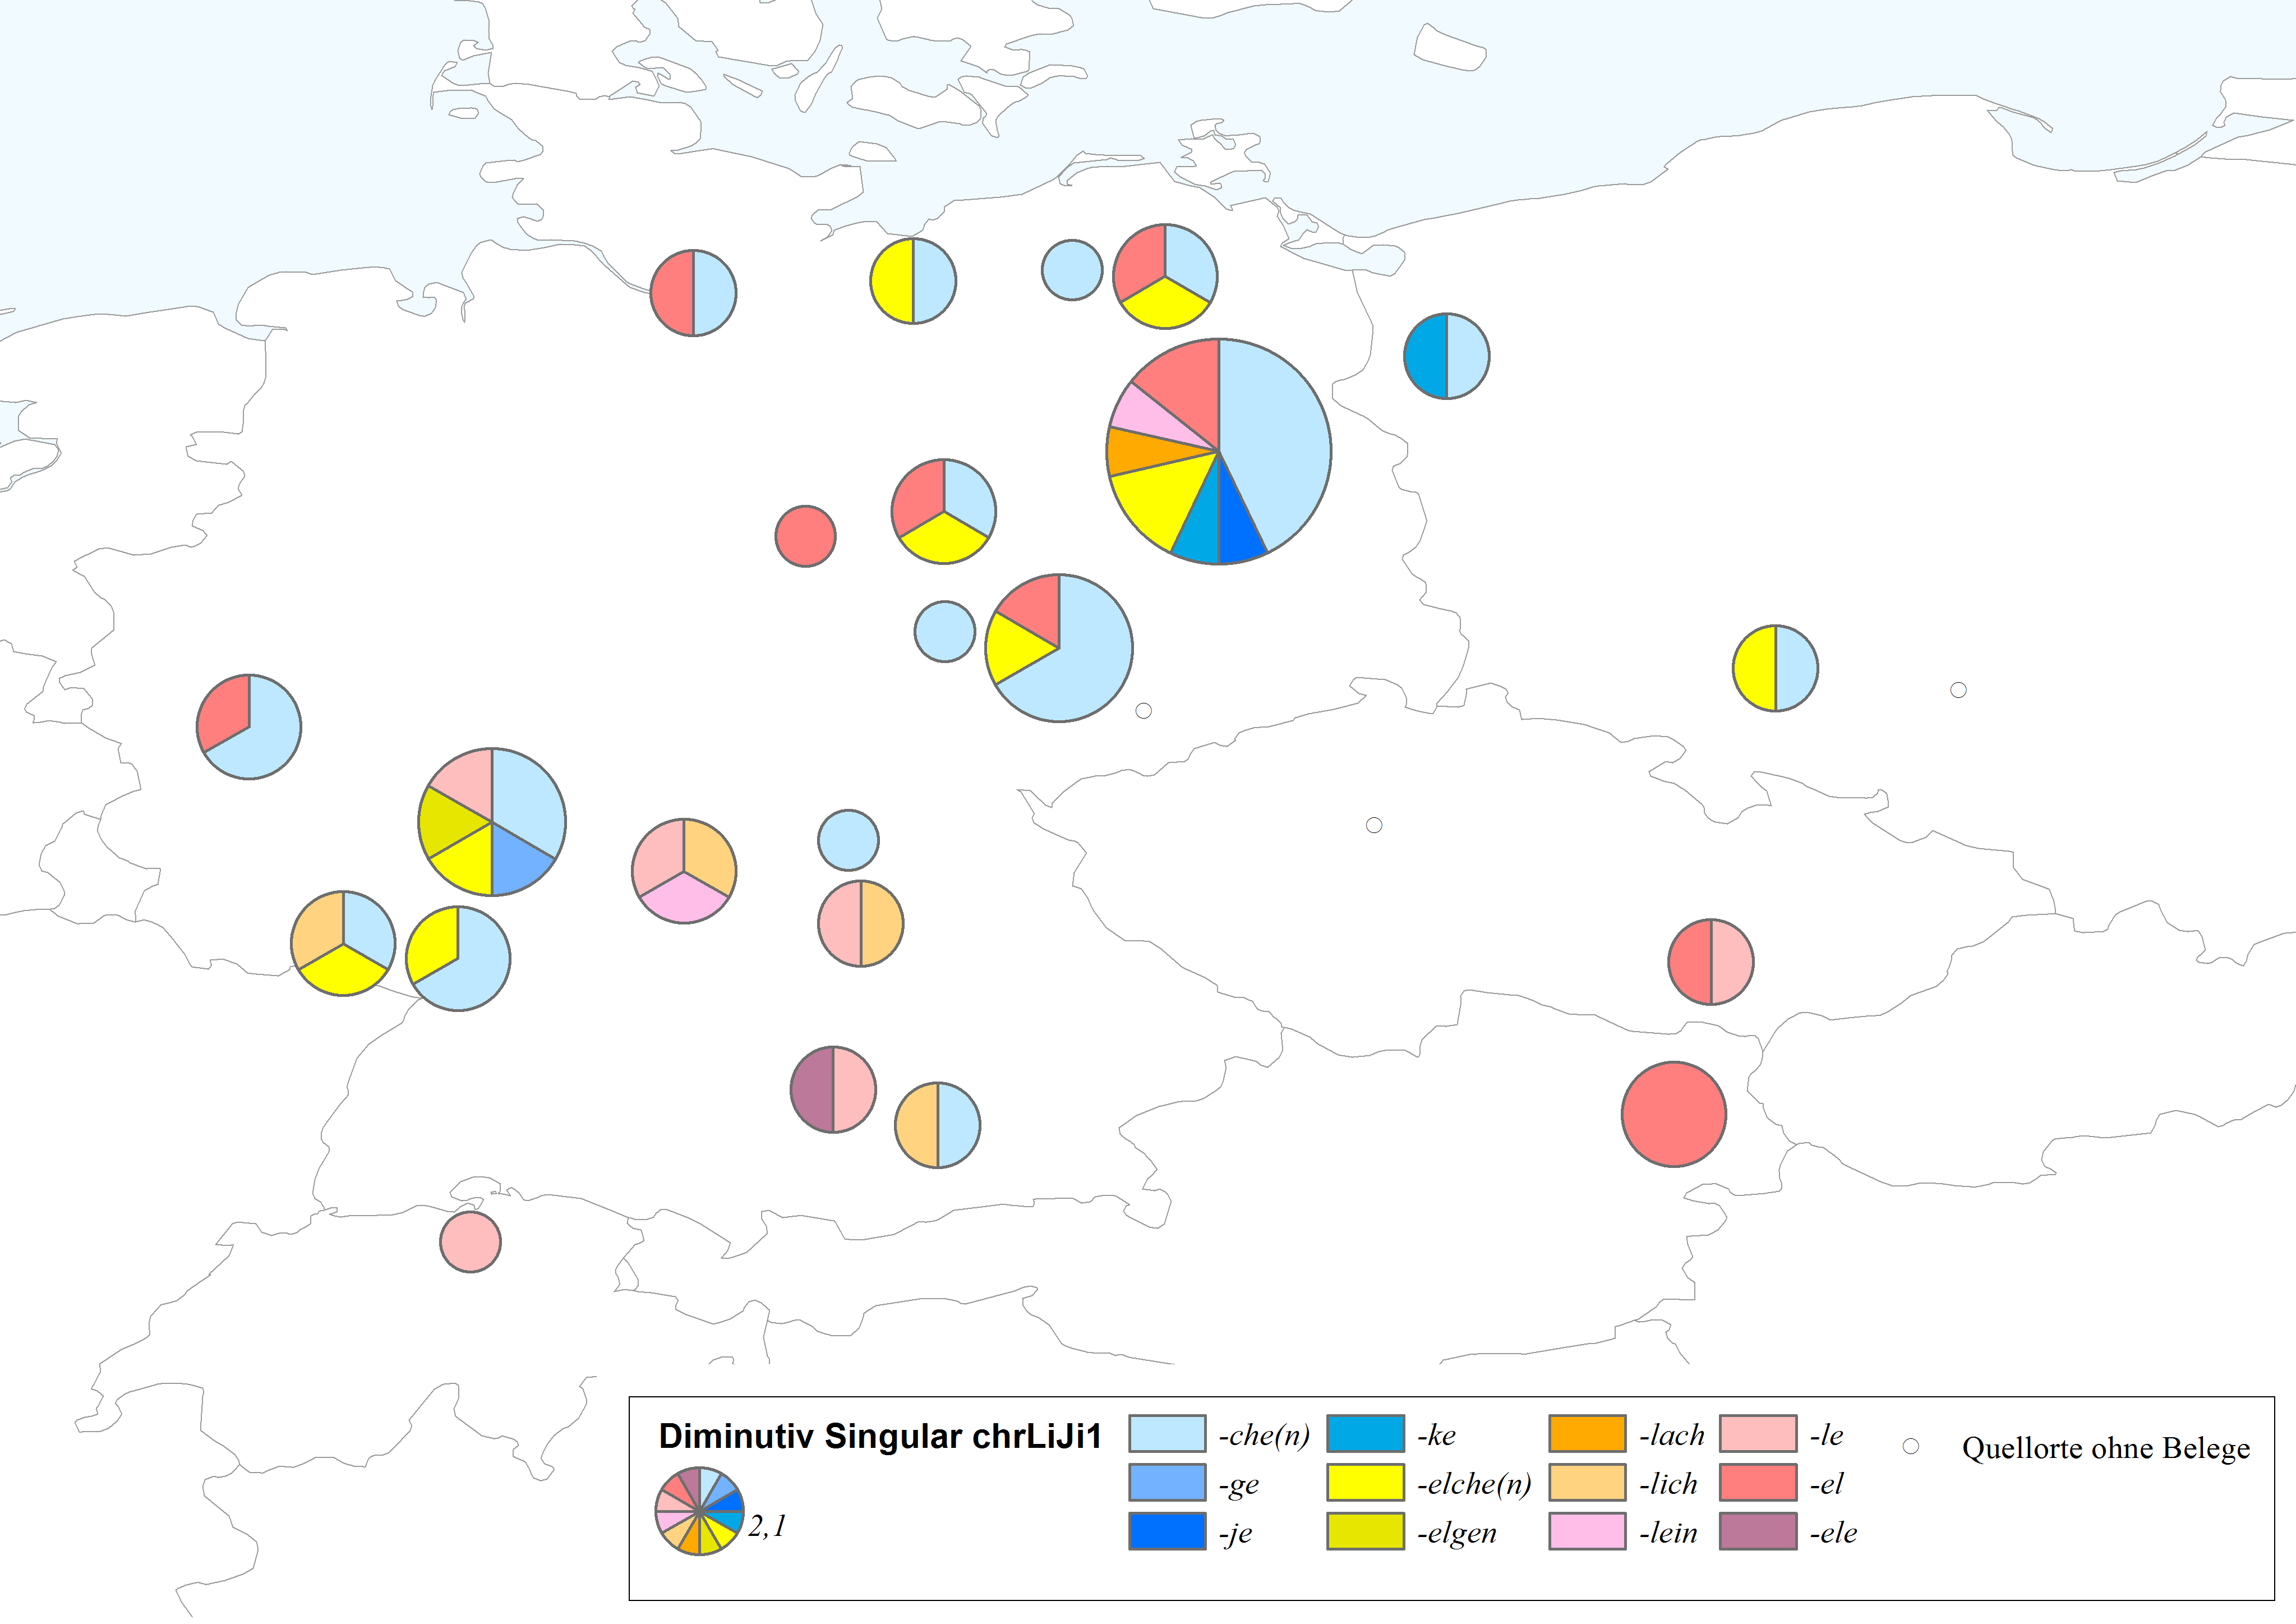
\includegraphics[scale=0.45]{figures/DIM_SG.png}
		\caption{\label{SgDimliji} Singulardiminutionen im \hai{chrLiJi1}}
		\end{figure} 
 

 \FloatBarrier  
 
 

\begin{figure}[h!]
\centering
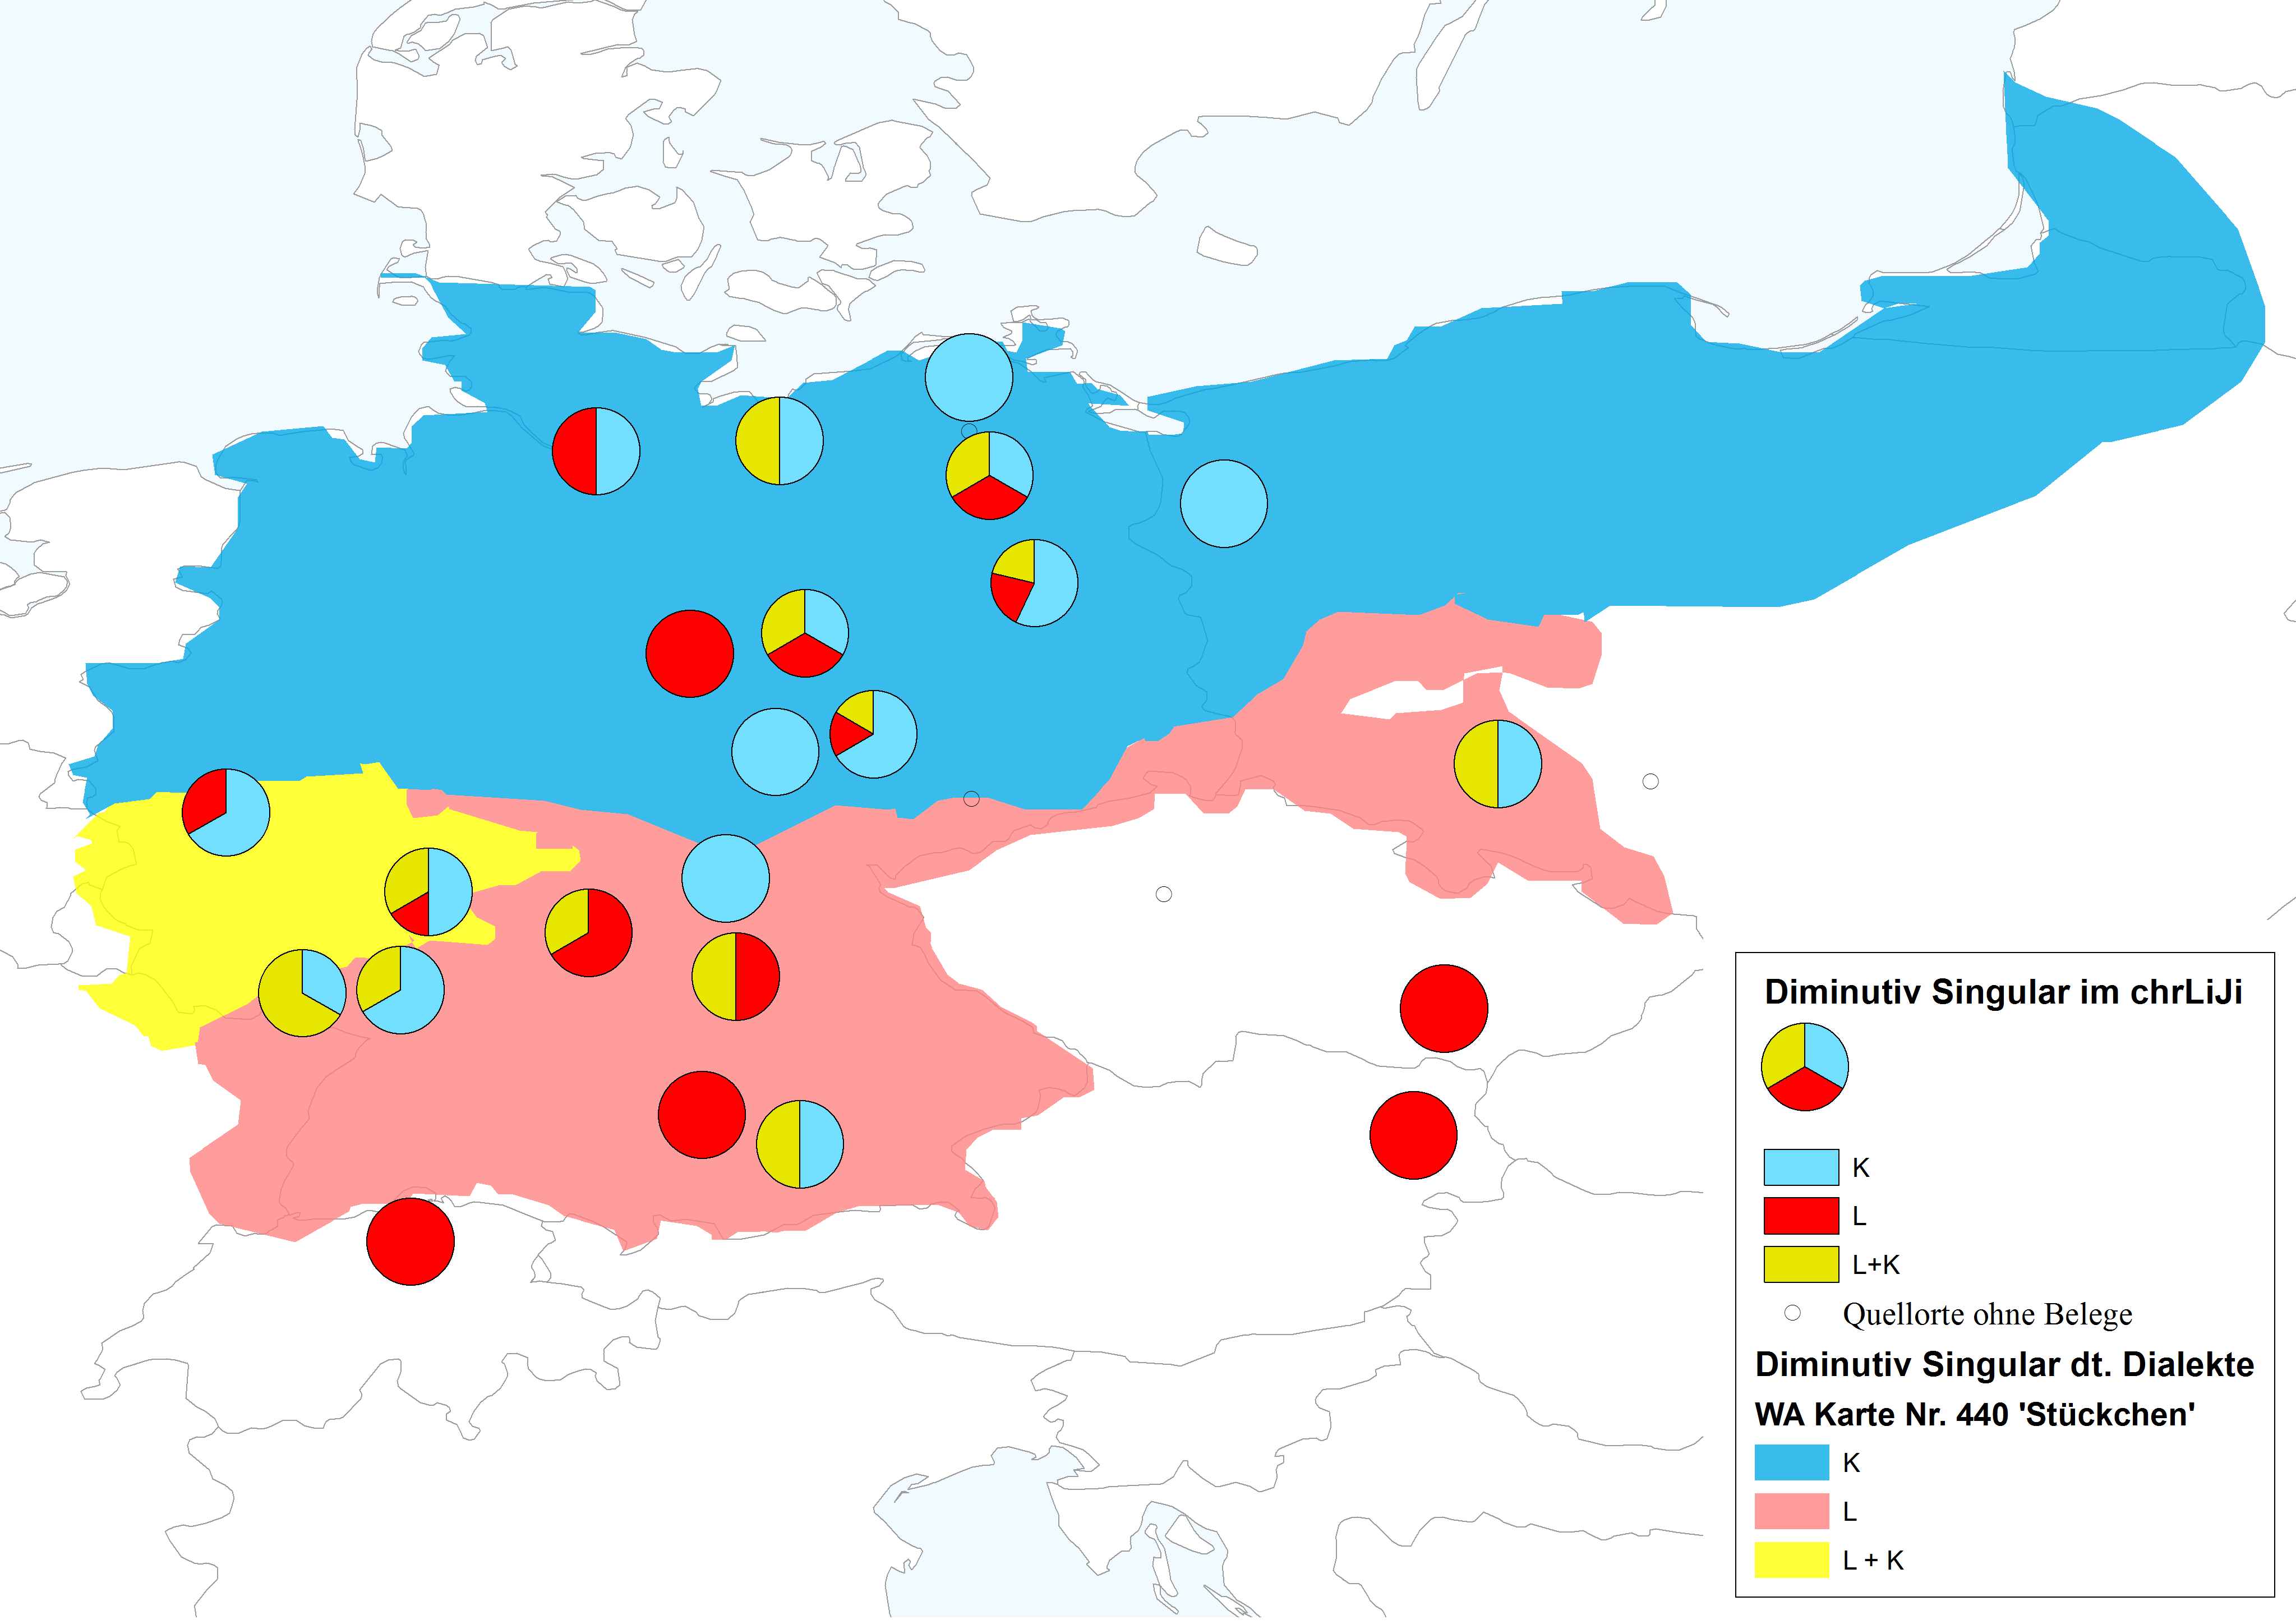
\includegraphics[scale=0.45]{figures/DIM_SG_DSA_DIM_SG_kurz.png}
		\caption{\label{SgDimDSAliji} Singulardiminutionen im \hai{chrLiJi1} und den dt. Dialekten (\hai{WA} Karte Nr. 440 \sem{Stückchen}) }
		\end{figure}
\FloatBarrier 

	
\begin{figure}[h!]
	\begin{tikzpicture}
		\begin{axis}[only marks, width=0.82\textwidth,height=0.4\textheight,
		legend style={at={(1,1)},xshift=0.2cm, yshift=-0.5cm,anchor=north west,nodes=left},
			%title={Funktionstypen des sp\"aten Westjiddisch},
			xtick={1700, 1725, 1750, 1775, 1800, 1825, 1850, 1875, 1900, 1925, 1950}, ytick=\empty,
			x tick label style={/pgf/number format/1000 sep=}, 
			y tick label style={/pgf/number format/1000 sep=},
			%extra y ticks={456.1, 1022.4},
			%extra y tick labels={{456,1},{1022,4}},
			extra y tick style={grid=major,
				tick label style={, ,}},
				ymin=0.2,
				ymax=6.2,
			ylabel={\hai{L}-Region  \hspace*{5mm} \hai{L + K}-Region  \hspace*{5mm} \hai{K}-Region},
			enlarge x limits=0.03]	
	
			%K-Gebiet
			\addplot [mark=square*, red] table [x=jahr, y=KDIML] {figures/KDIML.txt}; %1.4
			\addplot [ultra thick, mark=triangle*, yellow] table [x=jahr, y=KDIMLK] {figures/KDIMLK.txt}; %1
			\addplot [mark=o] table [x=jahr, y=KDIMK] {figures/KDIMK.txt}; %1.4

 \draw[gray!50] (-0.2cm,4.5cm) -- (15.5cm,4.5cm);		
			
			%LK-Gebiet
			\addplot [mark=square*, red] table [x=jahr, y=LKDIML] {figures/LKDIML.txt}; %1.4
			\addplot [mark=triangle] table [x=jahr, y=LKDIMLK] {figures/LKDIMLK.txt}; %1
			\addplot [mark=*, blue] table [x=jahr, y=LKDIMK] {figures/LKDIMK.txt}; %1.4
	 \draw[gray!50] (-0.2cm,2.5cm) -- (15.5cm,2.5cm);		
		
			%L-Gebiet

			\addplot [mark=square] table [x=jahr, y=LDIML] {figures/LDIML.txt}; %1.4
			\addplot [ultra thick, mark=triangle*, yellow] table [x=jahr, y=LDIMLK] {figures/LDIMLK.txt}; %1
			\addplot [mark=*, blue] table [x=jahr, y=LDIMK] {figures/LDIMK.txt}; %1.4


						\legend{\hai{L}-Dim., \hai{LK}-Dim., \hai{K}-Dim., \hai{L}-Dim., \hai{L + K}-Dim., \hai{K}-Dim.,\hai{L}-Dim., \hai{L + K}-Dim., \hai{K}-Dim.} 
		\end{axis}
	\end{tikzpicture}
	\caption{Regionale Verteilung von Singulardiminutionen im \hai{chrLiJi1}}
	\label{REGDIMSG}	
\end{figure}
\FloatBarrier



  
Im Plural zeigt sich hingegen folgendes Bild: 27 Quellen weisen eine \isi{Diminution} eines Plurals auf. Jedoch nur neun der Suffixe zeigen eine eigene morphologische Markierung des Plurals am Diminutivum (vgl. Tabelle \ref{tblDIMPL}).\footnote{\label{FNDIMPL}Diese Suffixe sind \textit{-cher}, \textit{-elcher}, \textit{-ercher}, \textit{-elger}; \textit{-chens}, \textit{-ches}, \textit{-ges}, \textit{-els} und \textit{-lich}. Je nach Ansatz ließe sich auch im Suffix -(\textit{ens})\textit{ke} eine Fussion aus \textit{en}-Plural mit \textit{s}-Plural und \hai{K}-\isi{Diminution} erkennen.} In vielen Fällen wird die Pluraldiminution mittels einer Addition des  \textit{-er}- oder \textit{-s}-\isi{Pluralsuffix} mit dem Diminutivsuffix vollzogen. Immerhin sechs Quellen setzen das jiddische Suffix \textit{-lich} ein (vgl. Fn. \ref{FNDIMPL}).\footnote{Die Quellen mit dem jiddischen Suffix \textit{-lich} sind: \hai{PG} (Speyer, 1835), \hai{PA} (Frankfurt, 1834), \hai{LM} (Würzburg, 1844), \hai{GP} (Nürnberg, 1831), \hai{SV} (München, 1890) und \hai{DG} (Wien, 1858).} Vier dieser Quellen (\hai{PA} Frankfurt, 1834, \hai{LM} Würzburg, 1844, \hai{GP} (Nürnberg, 1831) und \hai{SV} (München, 1890)) setzen dabei \textit{-lich} auch zur Singulardiminution ein. In diesen Fällen lässt sich von einer Hyperkorrektur des jiddischen Systems sprechen (vgl. S. \pageref{lichHyper} u. Karte in Abb. \ref{DimDSALiJilich}). Letzten Endes liegt damit in lediglich zwei Quellen des \hai{chrLiJi1} (\hai{PA} Frankfurt, 1834 u. \hai{DG} Wien, 1858) das tatsächliche jiddische Diminuierungssystem im Plural vor. Auffällig ist auch, dass die Belege zur Pluraldiminution mittels \textit{-lich} in relativer Nähe zu den Gebieten liegen, in denen laut \hai{WA}-Karte(n) dieses Suffix auch in den deutschen Dialekten üblich ist (vgl. \ref{DimDSALiJilich}). Damit ist nicht auszuschließen, dass dies eine Rolle bei den Imitationen gespielt hat. Zumindest ist es möglich, dass die Nähe zur deutschen Form die korrekte Verwendung der jiddischen Form erleichtert hat. 

Die Daten zur \isi{Diminution} im \hai{chrLiJi1} zeigen je nach Numerus unterschiedliche Raumstrukturen. Die nördlichen Quellen im \hai{K}-Gebiet sind, was die Singulardiminution betrifft, vielfältiger als der Süden oder die westliche Mitte (vgl. S. \pageref{sgDIMimNordenmehr}). Im Plural hingegen zeigen der Süden und die Mitte mehr Belege für eine gesonderte Pluralmarkierung am Diminutivsuffix als der Norden (vgl. Abb. \ref{Dimliji}).\\

 \begin{table}[h!]
		\begin{tabularx}{\columnwidth}{lXc}

		\hline 

\textbf{Suffix} &\textbf{Beispiel} & \textbf{Quellen} \\ \hline 


\textit{-che(n)} & \textit{Diminutivchen} \sem{Diminutiv\textsubscript{Dim. Pl.}} (\hai{PP}:\,27), \textit{Steinchen} \sem{Stein\textsubscript{Dim. Pl.}} (\hai{FS}:\,45, 73), \textit{Bäumchen} \sem{Baum\textsubscript{Dim. Pl.}} (\hai{PS}:\,28, 44) & 10 \\
 
  \textit{-cher} & \textit{Stickcher} \sem{Stück\textsubscript{Dim. Pl.}} (\hai{PA}:\,8, 17), \textit{Köpfcher} \sem{Kopf\textsubscript{Dim. Pl.}} (\hai{BS}:\,7),   \textit{Mädcher} \sem{Mädchen\textsubscript{Dim. Pl.}} (\hai{PL}:\,39, 50) & 6\\
 
  \textit{-chens} & \textit{Beinchens} \sem{Bein\textsubscript{Dim. Pl.}} (\hai{PP}:\,20), \textit{Mäuschens} \sem{Maus\textsubscript{Dim. Pl.}} (\hai{BW} Leipzig, 1826:\,108) & 4 \\
 
  \textit{-ches} & \textit{Semmelches} \sem{Brötchen\textsubscript{Dim. Pl.}} (\hai{BW} Leipzig, 1826:\,99, 105, 110), \textit{Banches } \sem{Bein\textsubscript{Dim. Pl.}} (\hai{PG}:\,44), \textit{Sternches} \sem{Stern\textsubscript{Dim. Pl.}} (\hai{JK}:\,11)& 5 \\
 
  \textit{-(ens)-ke} & \textit{Soldatenske} \sem{Soldat\textsubscript{Dim. Pl.}} (\hai{AJ}:\,1) & 1\\
 
  \textit{-ges} & \textit{Gesellschaftges} \sem{Gesellschaft\textsubscript{Dim. Pl.}} (\hai{PA}:\,23) & 1\\
 
 
  \textit{-elcher} & \textit{Stickelcher} \sem{Stück\textsubscript{Dim. Pl.}} (\hai{VD}:\,17), \textit{Jüngelcher} \sem{Junge\textsubscript{Dim. Pl.}} (\hai{PG}:\,17, 18, 19) & 2 \\
 
  \textit{-ercher} & \textit{Kindercher} \sem{Kind\textsubscript{Dim. Pl.}} (\hai{PG}:\,39, 43) & 1 \\
 
  \textit{-elger} & \textit{Schickselger} \sem{Nichtjude\textsubscript{Dim. Pl.}} (\hai{JK}:\,13), \textit{Jüngelger} \sem{Junge\textsubscript{Dim. Pl.}} (\hai{OF}:\,2) & 2 \\
 
  \textit{-lich} & \textit{Rädlich} \sem{Rad\textsubscript{Dim. Pl.}} (\hai{DG}:\,12), \textit{Büchlich} \sem{Buch\textsubscript{Dim. Pl.}} (\hai{SV}:\,V), \textit{Gänslich} \sem{Gans\textsubscript{Dim. Pl.}} (\hai{LM}:\,27)& 6\\
 
   \textit{-lein} & \textit{Äugelein} \sem{Auge\textsubscript{Dim. Pl.}} (\hai{LM}:\,27), \textit{Kindelein} \sem{Kind\textsubscript{Dim. Pl.}} (\hai{WA}:\,157) & 1 \\
  
         \textit{-el} & \textit{Schicksel} \sem{Nichtjüdin\textsubscript{Dim. Pl.}} (\hai{MV}:\,61) & 1 \\
    
        
    \textit{-els} & \textit{Schicksels} \sem{Nichtjüdin\textsubscript{Dim. Pl.}} (\hai{JP}:\,44) & 1 \\

 
 
  \hline 
 \end{tabularx}
		 \caption{Diminutivsuffixe Plural im \hai{chrLiJi1}}
		 \label{tblDIMPL}
		 \end{table}

  
   \FloatBarrier
  
  
  
   
   \begin{figure}[h!]
\centering
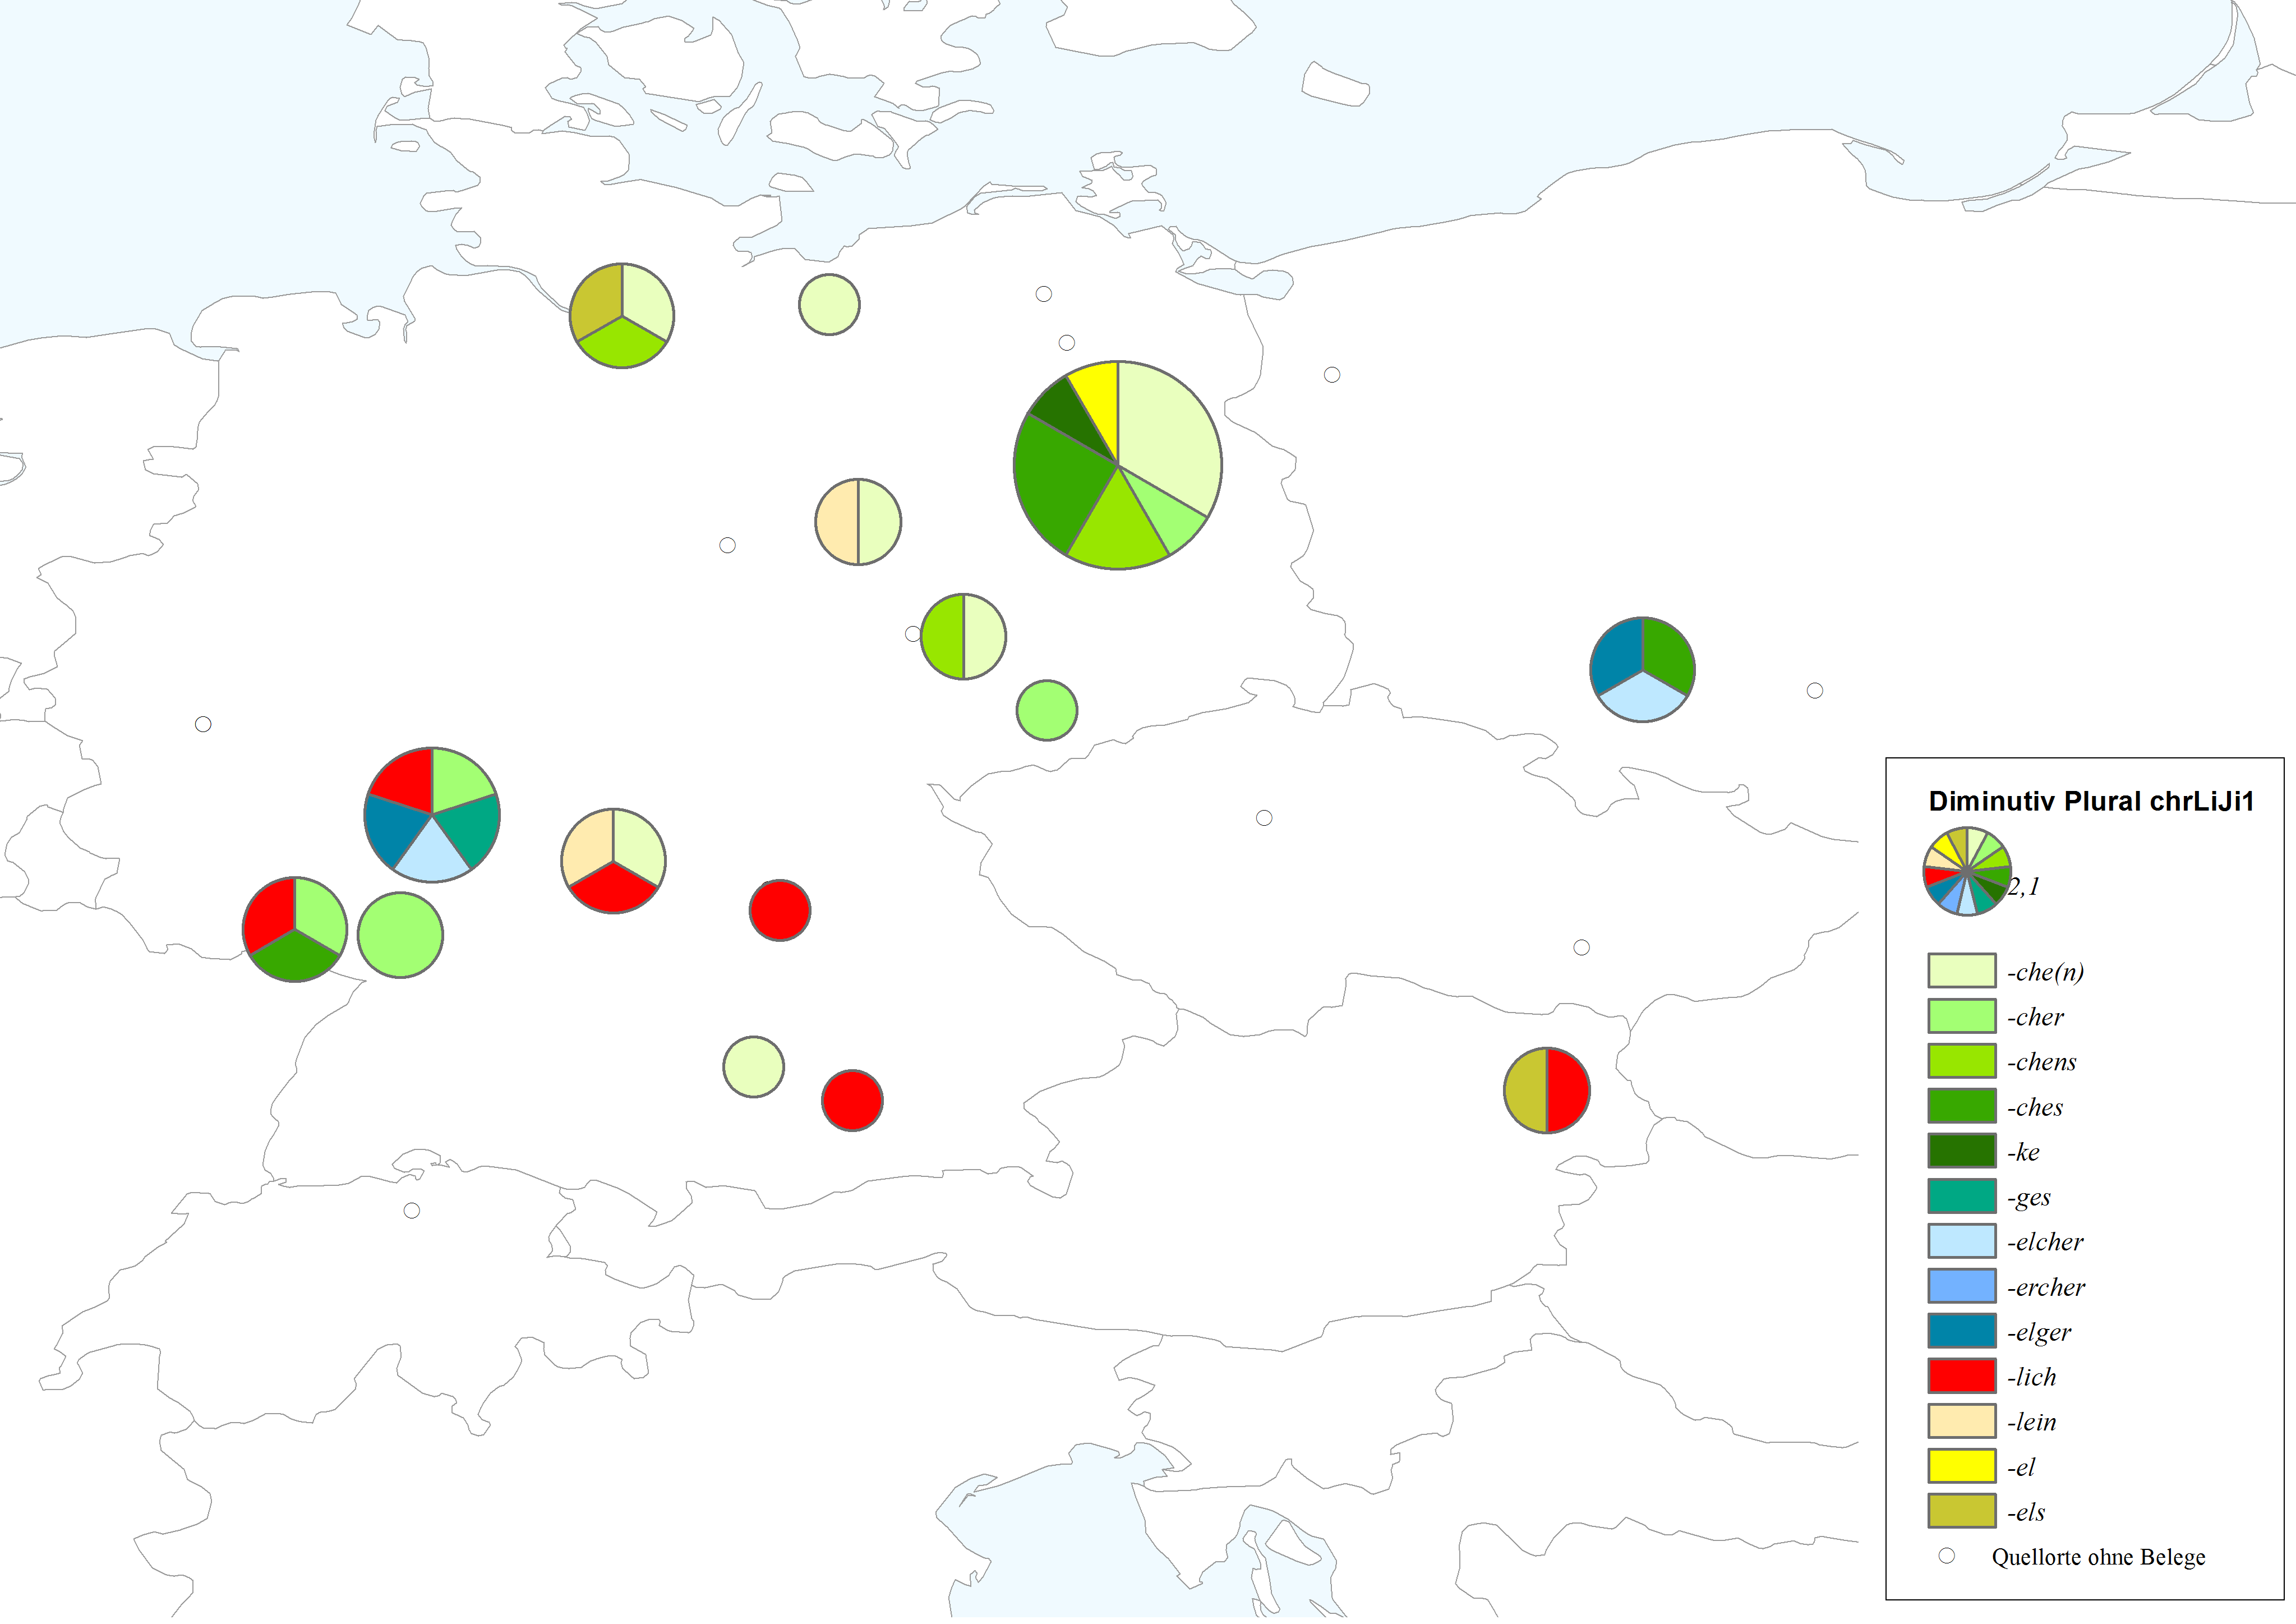
\includegraphics[scale=0.4]{figures/DIM_PL.png}
		\caption{\label{Dimliji} Pluraldiminutionen im \hai{chrLiJi1} (Einzelsuffixe)}
		\end{figure}  
  
  
  
  \begin{figure}[h!]
\centering
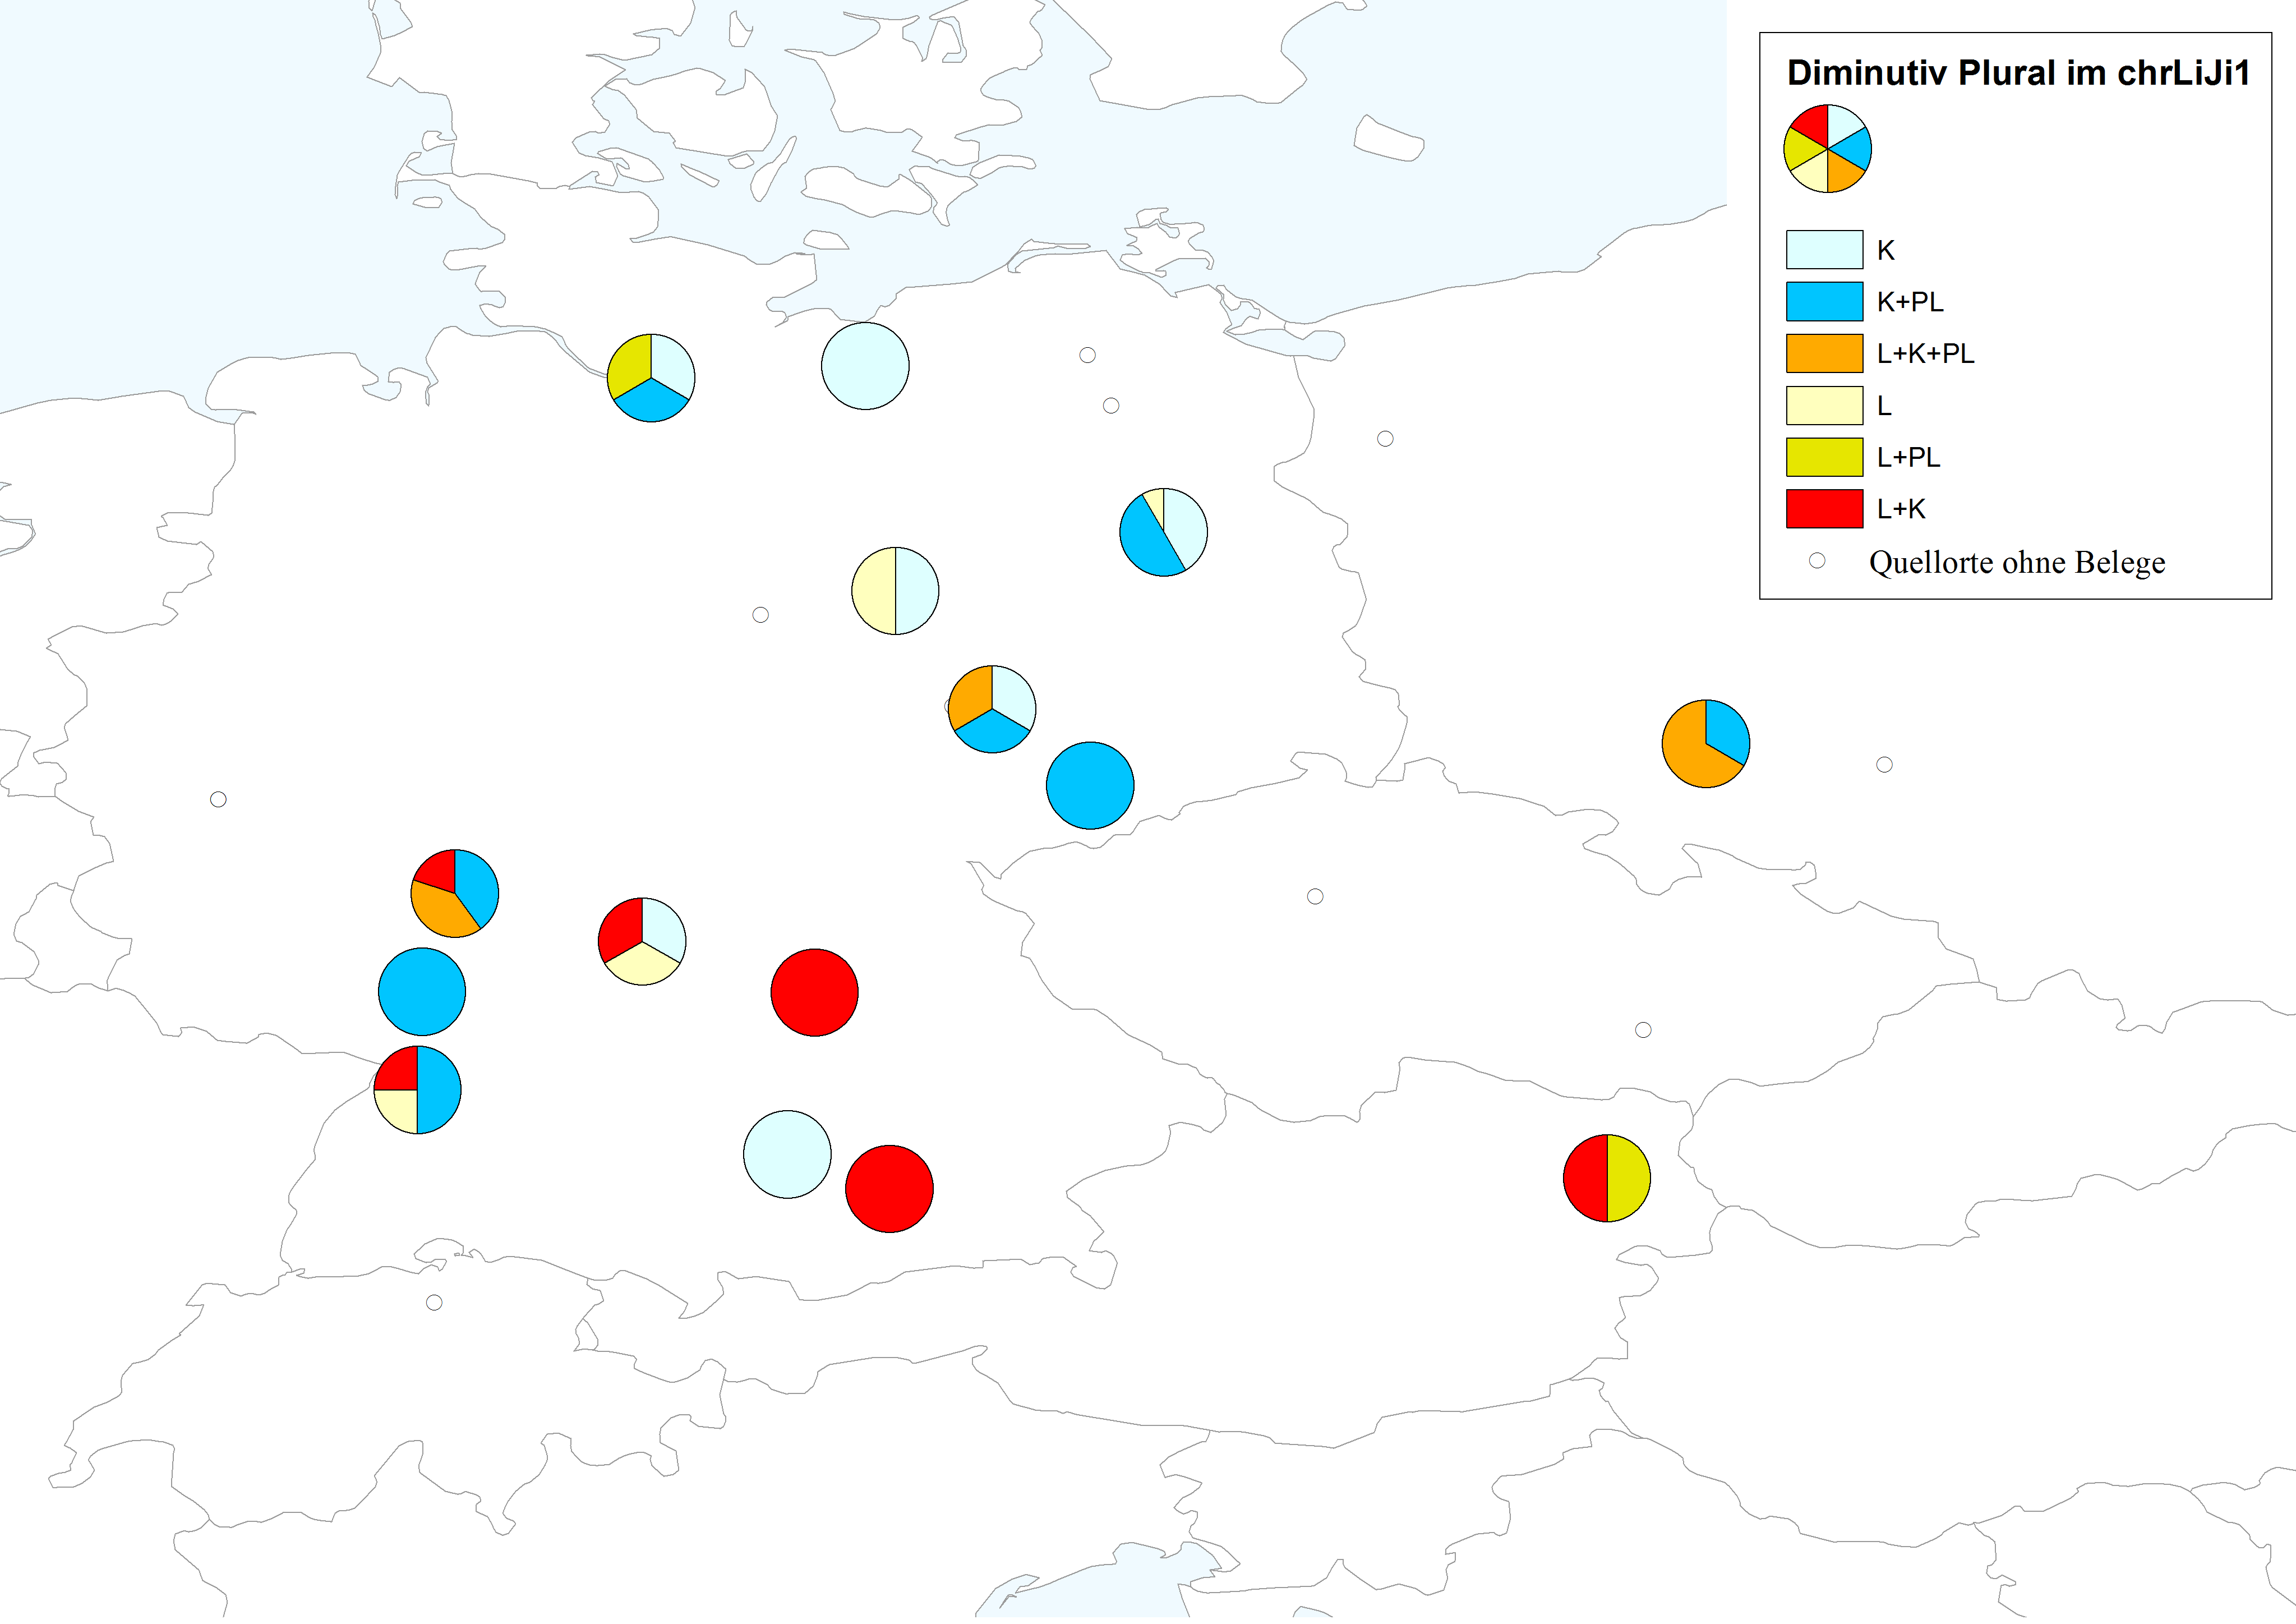
\includegraphics[scale=0.4]{figures/DIM_PL_kurz.png}
		\caption{\label{Dimlijikurz} Pluraldiminutionen im \hai{chrLiJi1} (Grundmuster)}
		\end{figure}  
  
   \FloatBarrier
 
 
  
 


  \begin{figure}[h!]
\centering
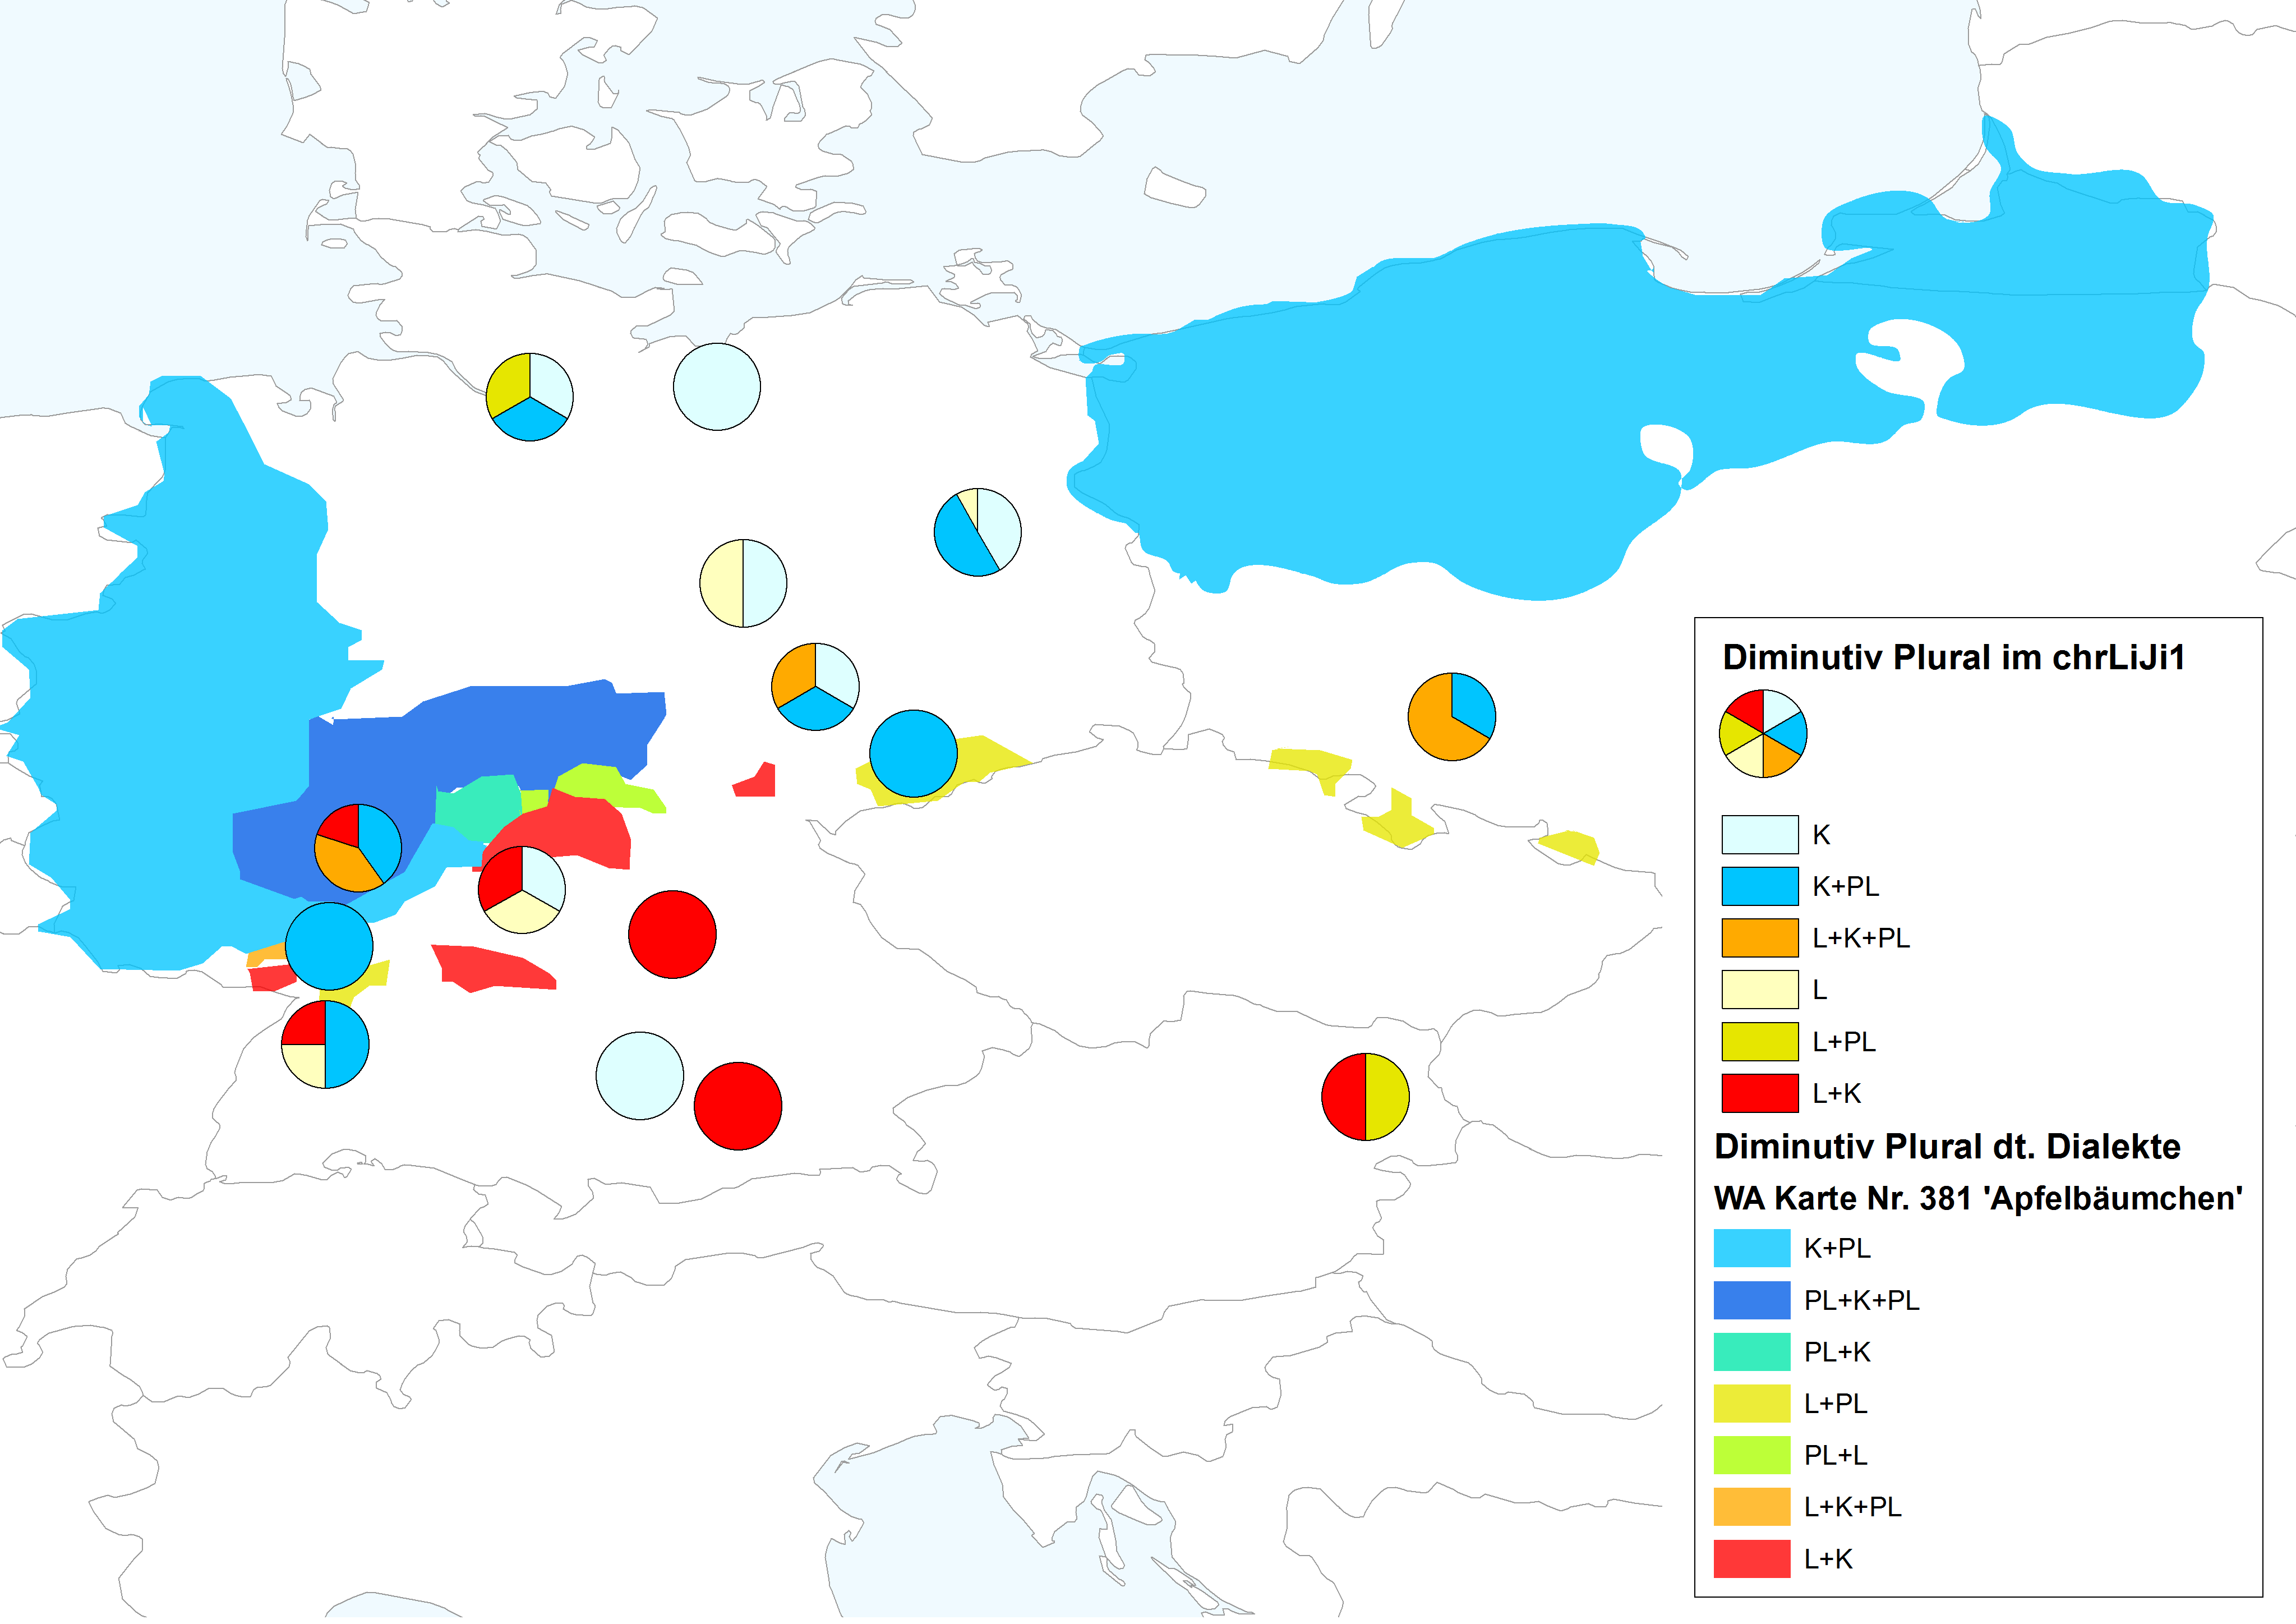
\includegraphics[scale=0.4]{figures/DIM_PL_DSA_Kurz.png}
		\caption{\label{DimDSALiJi} Pluraldiminutionen im \hai{chrLiJi1} und den dt. Dialekten (\hai{WA} Karte Nr. 381 \sem{Apfelbäumchen})}
		\end{figure}  
 \FloatBarrier



\begin{figure}[h!]
\centering
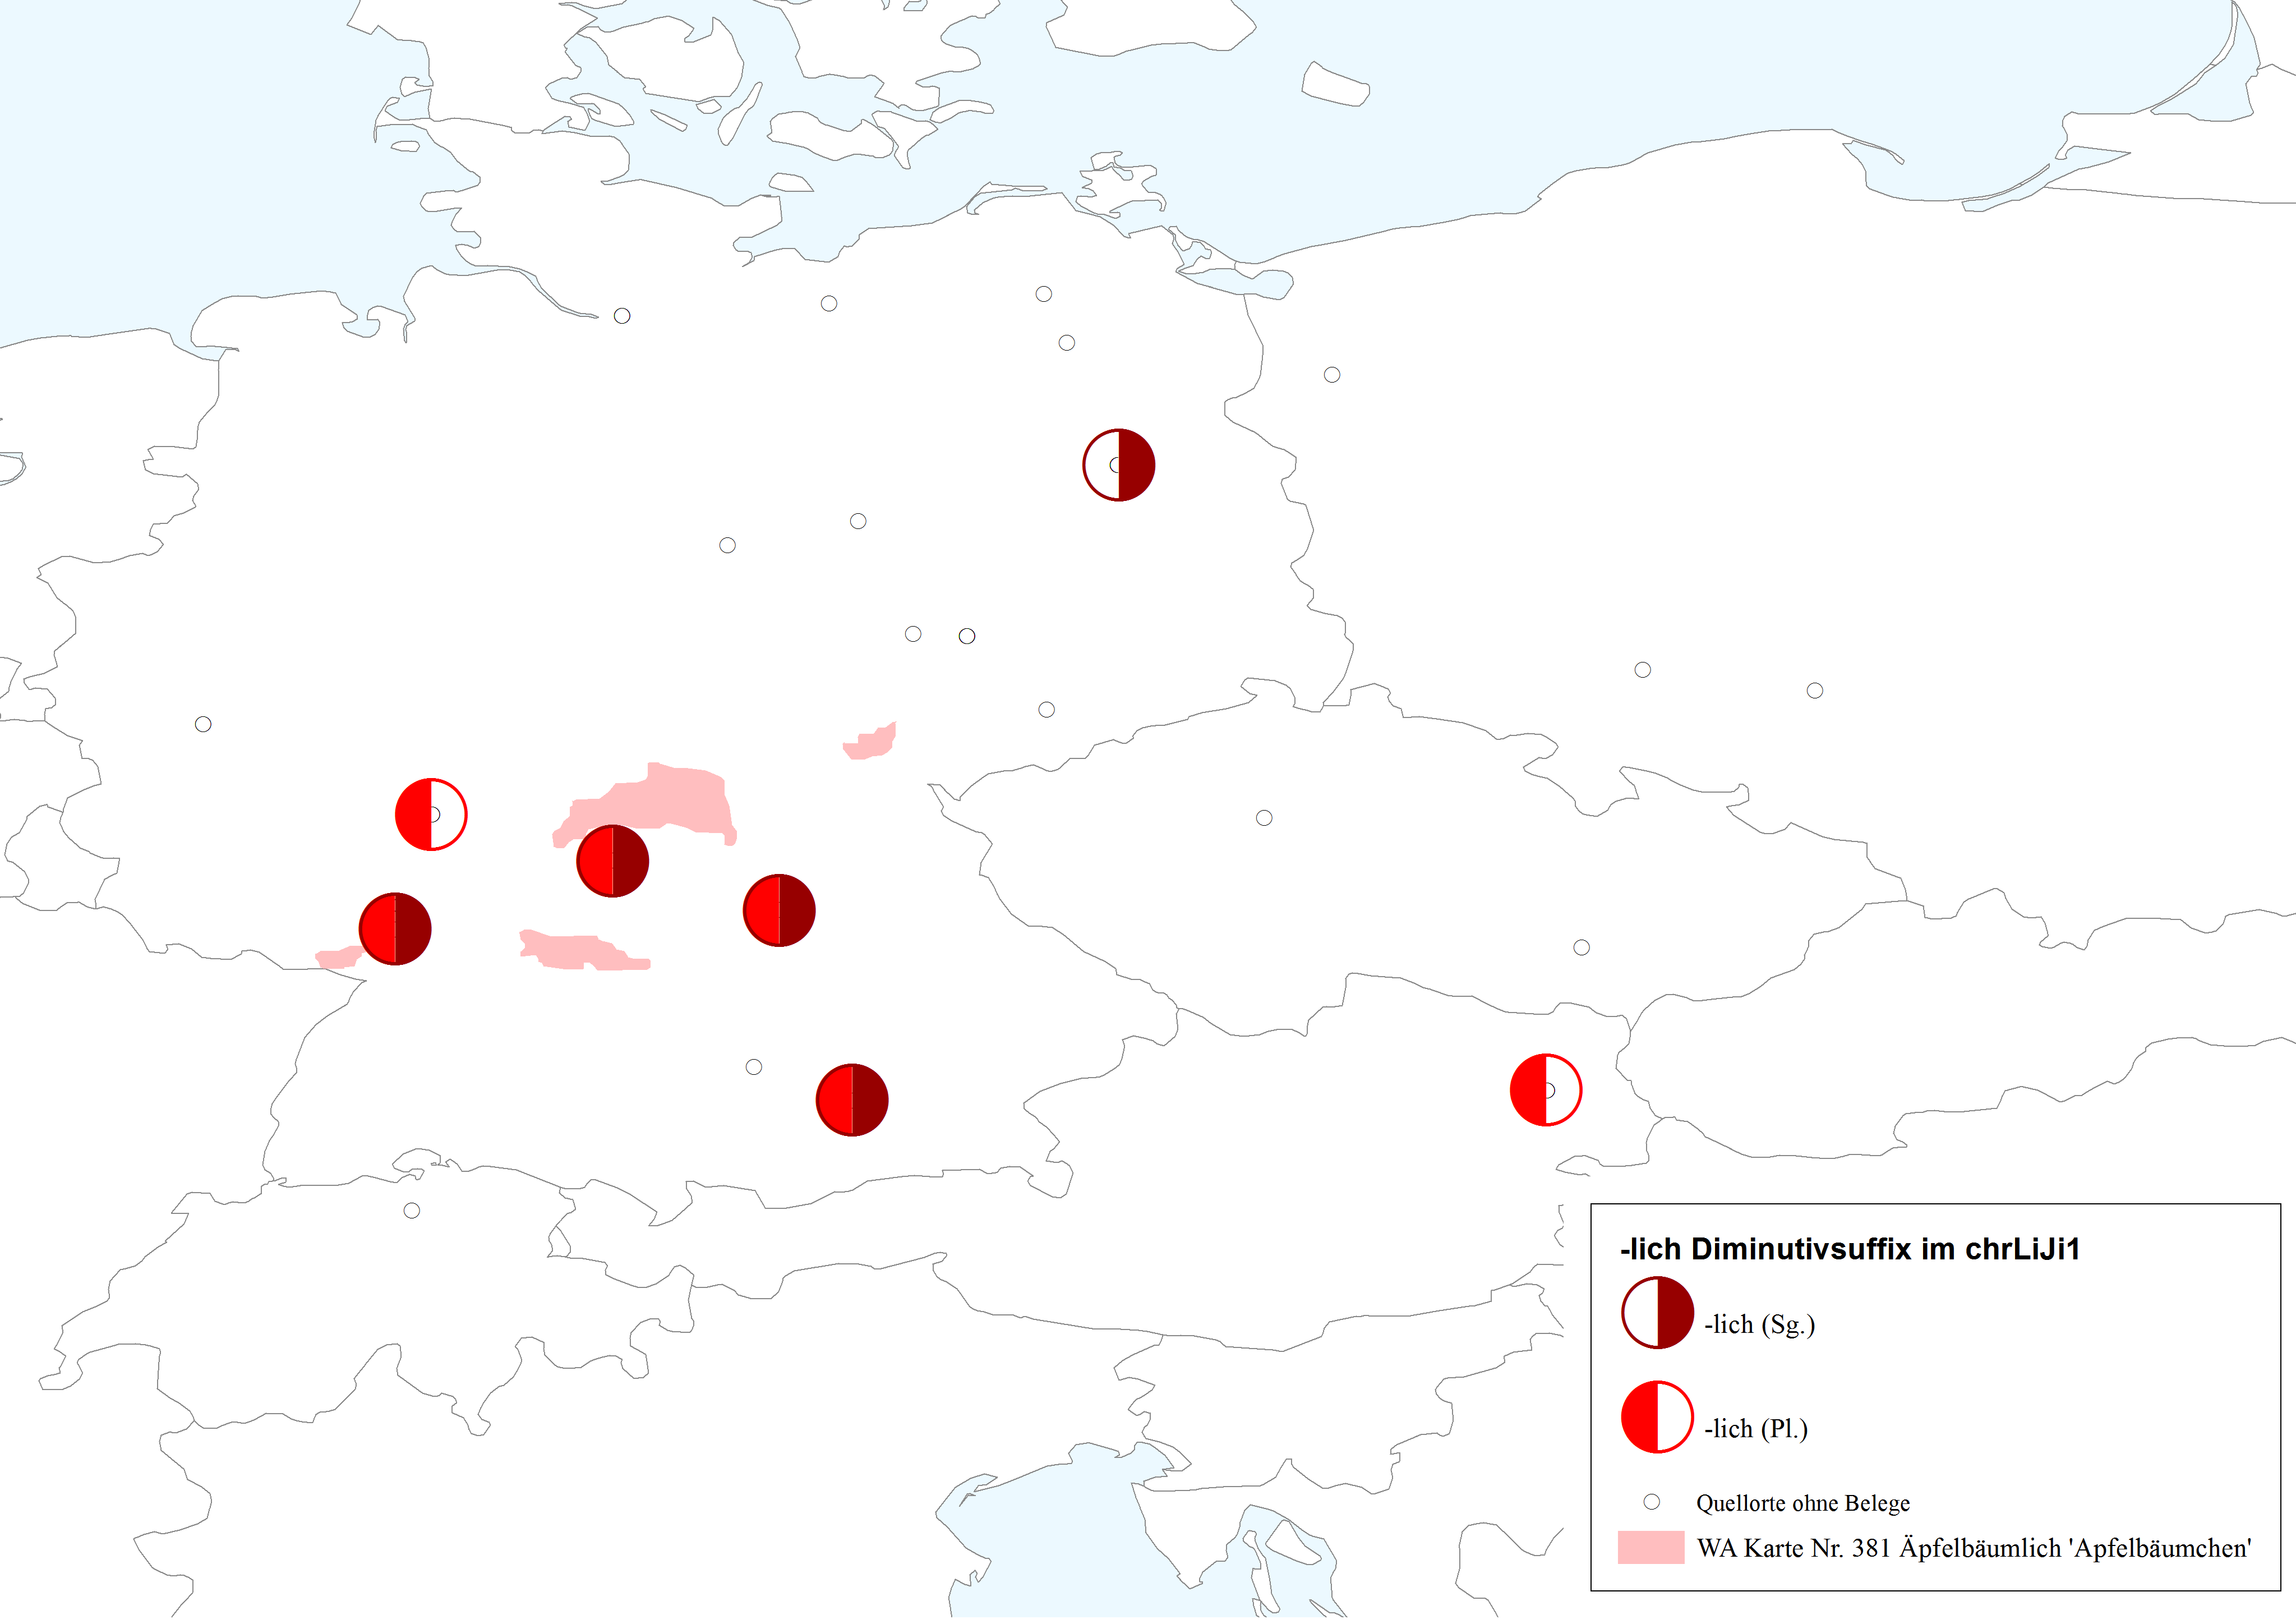
\includegraphics[scale=0.1]{figures/lich_Dim_pl_sg_DSA.png}
		\caption{\label{DimDSALiJilich} -\textit{lich}-Diminutionen im \hai{chrLiJi1} und den dt. Dialekten (\hai{WA} Karte Nr. 381 \sem{Apfelbäumchen})}
		\end{figure}
\FloatBarrier  


\subsection{\isi{Diminution} im \hai{jüdLiJi1} }\label{DIMjüdLiJi1}
%  %\noindent 
Auch im \hai{jüdLiJi1} findet sich eine Vielzahl an Diminutionen. Diese sind in allen der zehn untersuchten Texte belegt. Die Quellen aus Berlin (\hai{GuS1–23}, \hai{PBerlin1–2}) zeigen im Singular wie im Plural allesamt das schriftsprachliche Suffix \textit{-che(n)} (vgl. Tabelle \ref{tblDIMjüdliji1SG}). Die südlicheren Quellen verwenden hingegen \hai{L}-Diminutionen. Nur im Fall von \hai{PBreslau} finden sich alle drei Diminutionstypen (\hai{K}, \hai{L}, \hai{L + K}) parallel. 


  \begin{table}[h!]
		\begin{tabularx}{\columnwidth}{lXc}
\hline 
\textbf{Suffix} &\textbf{Beispiel} & \textbf{Quellen} \\ \hline 

\textit{-che(n)} & \textit{Lokomotivche} \sem{Lokomotive\textsubscript{Dim. Sg.}} (\hai{GuS1}:\,5), \textit{Liedche} \sem{Lied\textsubscript{Dim. Sg.}} (\hai{GuS5}:\,9), \textit{Geschäftchen} \sem{Geschäft\textsubscript{Dim. Sg.}}  (\hai{GuS23}:\,12), \textit{Demonschtratziönche} \sem{Demonstration\textsubscript{Dim. Sg.}} (\hai{PBerlin2}:\, 2.\,Sp.), \textit{Wörtche} \sem{Wort\textsubscript{Dim. Sg.}} (\hai{PBerlin1}:\,2) & 8 \\ 

 
 \textit{-elche} & \textit{Jüngelche} \sem{Junge\textsubscript{Dim. Sg.}} (\hai{PBreslau}:\,339) & 1 \\
 
 \textit{-le} & \textit{Schreibebriefle} \sem{Brief\textsubscript{Dim. Sg.}} (\hai{PAlsleben}:\,Titel, 3) & 1\\

 \textit{-el}/\textit{-l} & \textit{Päckel} \sem{Packet\textsubscript{Dim. Sg.}} (\hai{PBreslau}:\,342),  \textit{Stückel} \sem{Stück \textsubscript{Dim. Sg.}} (\hai{PDebrecen}:\,7, 13) & 2 \\
 
 \textit{-ele} & \textit{Büchele} \sem{Buch\textsubscript{Dim. Sg.}} (\hai{PDebrecen}:\,9),  \textit{Haisele} \sem{Hase \textsubscript{Dim. Sg.}} (\hai{PDebrecen}:\,13) & 1 \\ 
 
     \hline 
 \end{tabularx}
		 \caption{Diminutivsuffixe Singular im \hai{jüdLiJi1}}
		 \label{tblDIMjüdliji1SG}
		 \end{table}


  \begin{table}[h!]
		\begin{tabularx}{\columnwidth}{lXc}

		\hline 

\textbf{Suffix} &\textbf{Beispiel} & \textbf{Quellen} \\ \hline 
  \textit{-cher} & \textit{Ameischer} \sem{Ameise\textsubscript{Dim. Pl.}} (\hai{GuS1}:\,3),  \textit{Perzentcher} \sem{Prozent\textsubscript{Dim. Pl.}} (\hai{GuS5}:\,7),  \textit{Schwebelhölzcher} \sem{Schwefelholz\textsubscript{Dim. Pl.}} (\hai{GuS10}:\,5), \textit{Tröppcher} \sem{Tropfen\textsubscript{Dim. Pl.}} (\hai{PBerlin1}:\,2)  & 4 \\

  \textit{-che(n)} & \textit{Kreppchen} \sem{Krapfen\textsubscript{Dim. Pl.}} (\hai{GuS15}:\,3), \textit{Bettchen} \sem{Bet\textsubscript{Dim. Pl.}} (\hai{PBerlin1}:\,2), \textit{Affzierche} \sem{Offizier\textsubscript{Dim. Pl.}} (\hai{PBerlin2}:\,1.\,Sp.) & 3 \\

 
  \textit{-chers} & \textit{Offißierchers} \sem{Offizier\textsubscript{Dim. Pl.}} (\hai{PBerlin2}:\,2.\,Sp.) & 1 \\
 
 
  \textit{-ercher} & \textit{Gesetzercher} \sem{Gesetz\textsubscript{Dim. Pl.}} (\hai{PBerlin1}:\,4) & 1 \\
 
   \textit{-che(n)s} & \textit{Bäckches} \sem{Backe\textsubscript{Dim. Pl.}} (\hai{PBerlin1}:\,2), \textit{Kupperhütchens} \sem{Kupferhut\textsubscript{Dim. Pl.}} (\hai{GuS10}:\,10) & 3 \\
   
   \textit{-lech} & \textit{Jidlech} \sem{Jude\textsubscript{Dim. Pl.}} (\hai{PDebrecen}:\,7),  \textit{Zeitungblättlech} \sem{Zeitungsblatt\textsubscript{Dim. Pl.}} (\hai{PDebrecen}:\,14)  & 1 \\
  
 \hline 
 \end{tabularx}
		 \caption{Diminutivsuffixe Plural im \hai{jüdLiJi1}}
		 \label{tblDIMjüdliji1PL}
		 \end{table}

 
    
    Besonders authentisch bezüglich der \isi{Diminution} präsentiert sich \hai{PDebrecen}, wo wir den einzigen Beleg einer Pluraldiminution mittels \textit{-lech} finden. Bemerkenswert daran ist, dass wir hier bereits die ostjiddische Vokalisierung des Suffixes antreffen und nicht die westjiddische (\textit{-lich}), wie sie im \hai{chrLiJi1} belegt ist. In den \hai{GuS1–10} finden wir ausschließlich die Pluralsuffixe \textit{-cher} und \textit{-chen} (vgl. Tabelle \ref{tblDIMjüdliji1PL}). Eine besondere Vielfalt an Diminutionssuffixen im Plural findet sich in \hai{PBerlin1} (\textit{-chen}, \textit{-ches}, \textit{-ercher}, \textit{-chers}) und \hai{PBerlin2} (\textit{-che}, \textit{-ches}, \textit{-chens}). Diese Suffixe funktionieren nach dem Prinzip \hai{K}+\hai{Pl.} (bzw. in einem Fall \hai{Pl.}+\hai{K}+\hai{Pl.}) und bauen damit auf die \hai{K}-\isi{Diminution} auf. Es findet sich, vom \textit{-lech}-Beleg aus \hai{PDebrecen} abgesehen, kein einziger Beleg für Pluraldiminutiva der Fusionsformen, wie wir sie im \hai{chrLiJi1} besonders im Nordosten finden (vgl. S. \pageref{LKinberlin}). Hierin besteht also ein deutlicher Unterschied zwischen \hai{chrLiJi1} und \hai{jüdLiJi1}. 

Zusammenfassend lässt sich feststellen, dass im \hai{jüdLiJi1} weniger Aufwand betrieben wurde, Suffixe zu wählen, die nicht der örtlichen deutschen \isi{Diminution} entsprechen, als es im \hai{chrLiJi1} der Fall ist. Das Besondere an den Belegen zur \isi{Diminution} im \hai{jüdLiJi1} ist, dass diese vergleichbar hoch frequent sind wie im \hai{chrLiJi1}. Es ist also vielmehr die reine Präsenz von \isi{Diminution} als deren konkrete morphologische Struktur, die die Gemeinsamkeit beider Formen des \hai{LiJi1} ausmacht. Diminutive können durch die ironische, scherzhafte Funktion des \hai{C2}-Typs provoziert sein und wären damit textsortenspezifisch. Mit Blick auf die Situation im \hai{chrLiJi1} liegt es jedoch nahe, \isi{Diminution} als figurenspezifisch \quein{jüdisch} anzusehen. 

Darüber hinaus bestärken die Belege aus dem \hai{jüdLiJi1} die Vermutung, dass die Diminutionsmorphologie (insbes. Singulardiminution) im Westjiddischen vielfältig ist und kleinräumige regionale Muster anzunehmen sind. Doch für weitere Ergebnisse dieser Art ist das \isi{Korpus} zum \hai{jüdLiJi1} zu klein und die geographische Streuung der Quellen (auch die aller potentieller Quellen) zu gering. \\

 \subsection{Funktionen von \isi{Diminution} im \hai{LiJi} }\label{DIMFunktionen}
%  %\noindent
   Die Funktion der Diminutivsuffixe im \hai{chrLiJi1} ist schwer auszumachen. Zum einen ist es möglich, dass mit ihnen  eine tatsächliche Sprachrealität abgebildet wird, die aufgrund der dünnen Quellenlage nicht klar umrissen werden kann, zum anderen aber sind die Formen areal und diachron zu wahllos verbreitet, als dass dies Rückschlüsse auf feinere Strukturen zuließe. Was grobe Raumstrukturen betrifft, so bieten die Daten des \hai{chrLiJi1} immerhin Ansätze für weitere Untersuchungen. Durch authentische Quellen zu prüfen wären besonders die Hypothesen, dass \hai{L+K}-Fusionsformen im Singular im Nordosten des Westjiddischen verbreitet waren oder dass die Pluraldiminution mittels -\textit{lich} lediglich im Süden des Sprachgebiets tatsächlich verwendet wurde, während im Norden andere, auf \hai{K}-Diminutionen aufbauende Formen, präsent waren.\\


Die Analyse hat gezeigt, dass sich die Quellen des \hai{jüdLiJi1}  ähnlich den koterritorialen Quellen des \hai{chrLiJi1} verhalten. Andererseits irritiert besonders, dass wir im \hai{chrLiJi1} eine solch große Variation an Suffixen vorfinden, die uns aus den jiddischen Varietäten nicht bekannt ist (vgl. Abschnitt \ref{dimJIDDISCH}) und auch nicht durch Daten des \hai{jüdLiJi1} bestätigt wird. Hinzu kommt, dass sich \isi{Diminution} außerhalb des \hai{LiJi} als Charakteristikum der jiddischen Sprache etabliert haben muss, anders ist nicht zu erklären, warum sie bereits vielfach in den frühesten Quellen belegt ist (vgl. Abb. \ref{REGDIMSG}). Dies spricht dafür, anzunehmen, dass \isi{Diminution} an sich, also unabhängig der morphologischen Struktur des Suffixes, besonders stark als grammatische Kennfunktion \textit{jüdischer Sprache} agiert. Um ein besseres Bild der Funktionen von \isi{Diminution} im \hai{LiJi} zu gewinnen, bedarf es allerdings weiterer Daten der gesprochenen und geschriebenen Sprache. Erst dann könnte geklärt werden, ob ein äußerst hoher Gebrauch an Diminutiva tatsächlich der jiddischen Sprachrealität entspricht oder nicht. 

 \section{Plurale}\label{pl}
 %\noindent
In einigen Fällen weist das \hai{LiJi} Pluralformen auf, die vom Schriftdeutschen abweichen. Besonders populär ist dabei die Verwendung des  \textit{s}-Plurals (vgl. Unterabschnitte \ref{sPlural} u. \ref{sPluralLiJi}). Eine weitere, jedoch deutlich seltener auftretende Pluralmorphemalternanz wird in Unterabschnitt \ref{erPLURAL} vorgestellt. Bevor auf die Daten zum \hai{LiJi} näher eingegangen wird, gibt der nachfolgende Unterabschnitt \ref{plDEUJI} einen allgemeinen Überblick zu den Grundmustern der Pluralbildung im Jiddischen und Deutschen. \\


 
\subsection{Grundmuster der Pluralmorphologie im Jiddischen und Deutschen}\label{plDEUJI}
%  %\noindent 
 Das Pluralsystem in den deutschen Dialekten ist alles andere als einheitlich. Nicht nur, dass dialektale Variation bei der Wahl der Pluralisierungsstrategie vorliegt, sondern es gibt  in den Dialekten  Strategien, wie z.\,B. Pluralmarkierung durch \isi{Subtraktion} (vgl. \cite{GolstonWiese1996}; \cite{HolsingerHouseman1999}; \cite{Knaus2003}; \cite{BirkenesDiss}), die die Schriftsprache nicht kennt (vgl. \cite[414–443]{Schirmunski1962}; \cite{Nuebling2005}; \cite[insbes. 155–169]{Wiese2009}). Pluralisierung im Jiddischen folgt in den meisten Fällen Strategien, die auf die germanische Komponente zurückgehen. Der Plural wird überwiegend nach den folgenden Prinzipien gebildet: -\textit{er}, -\textit{(e)n}, -\textit{∅},  -\textit{(e)s},\footnote{Ob sich die Existenz eines \textit{s}-Plurals im Jiddischen auf die alt- bzw. mittelhochdeutsche Komponente zurückführen lässt, ist anzweifelbar (vgl. etwa \cite{King1990}; \cite{Timm2007}). Da es aber eine Strategie ist, die germanischen Sprachen nicht fremd ist, wird es hier dennoch angeführt. Denn selbst wenn der \textit{s}-Plural im Jiddischen nicht genuin deutschen Ursprungs ist, so wird das germanische Grundgerüst des Jiddischen, welches einen alt-/mittelhochdeutschen Ursprung hat, die Aufnahme dieses Plurals begünstigt und katalysiert haben. Weiter ist zu sagen, dass der einfache -\textit{e}-Plural ± \isi{Umlaut} im Jiddischen durch die \isi{Apokope} abgebaut wurde (\cite[29]{Timm2007}).\label{FNsplural}} ± \isi{Umlaut} (Bsp. \ref{PLji1erUmlaut}–\ref{PLji1nurUmlaut} zitiert n. \cite[163]{Jacobs2005}). Hinzu kommt die aus der \ili{hebräisch}-aramäischen Komponente stammende Pluralbildung mittels  -\textit{im}/ -\textit{em}, die überwiegend auf Lexeme dieser Komponente angewendet wird (Bsp. \ref{PLji1Hebr} zitiert n. \cite[165]{Jacobs2005}) und nur in wenigen Ausnahmefällen Lexeme anderer Komponenten betrifft (Bsp. \ref{PLji1Hebrgerm} zitiert n. \cite[165]{Jacobs2005}). Wie bereits gezeigt, verfügt das Jiddische über eine gesonderte Pluralbildung im Rahmen der \isi{Diminution} (vgl. Abschnitt \ref{dim}).

Wie in den deutschen Dialekten, so gibt es auch in den jiddischen Dialekten areale Variation (Bsp. \ref{PLji1dialekt}). Zur Situation in den westjiddischen Dialekten fehlt es noch an Detailanalysen, es ist aber anzunehmen,  dass dort ebenso wie in den deutschen und ostjiddischen Dialekten diatopische Variation zu erwarten ist, welche u.\,U. sogar parallel zu denen der deutschen Dialekte liegt. So finden wir etwa in einer unserer ältesten Quellen des gesprochenen Westjiddischen, der \qu{Hochzeit zu Grobsdorf}, bereits  Belege für Interferenzen mit den örtlichen hessischen Dialekten, wo der \textit{-er}-Plural besonders \isi{produktiv} ist (\ref{PLWJgrob}; vgl. \cite[83]{Friebertshaeuser1987}). \\


 \eenumsentence{
 \item Sg. \RL{לא\makebox(-1.5,-7.5)[r]{\libertineGlyph{uni207B}}נד} \textit{land} \sem{Land} – Pl. \RL{לענדער} \textit{lender} \sem{Länder} \label{PLji1erUmlaut} 
 \item Sg. \RL{וו{יי}\makebox(-1.5,-7.5)[r]{\libertineGlyph{uni207B}}ב} \textit{vayb} \sem{Weib, Frau} – Pl. \RL{וו{יי}\makebox(-1.5,-7.5)[r]{\libertineGlyph{uni207B}}בער} \textit{vayber} \sem{Weiber, Frauen} \label{PLji1nurer}
 \item Sg. \RL{ט{יי}\makebox(-1.5,-7.5)[r]{\libertineGlyph{uni207B}}ך} \textit{taykh} \sem{Fluss} – Pl. \RL{ט{יי}\makebox(-1.5,-7.5)[r]{\libertineGlyph{uni207B}}כן} \textit{taykhn} \sem{Flüsse} \label{PLji1n} 
  \item Sg. \RL{זינגער} \textit{zinger} \sem{Sänger} – Pl. \RL{זינגערס} \textit{zingers} \sem{Sänger} \label{PLji1s} 
 \item Sg. \RL{הא\makebox(-1.5,-7.5)[r]{\libertineGlyph{uni207B}}נט} \textit{hant} \sem{Hand} – Pl. \RL{הענט} \textit{hent} \sem{Hände} \label{PLji1nurUmlaut}
 \item Sg. \RL{למדן} \textit{lamdn} \sem{Gelehrter} – Pl. \RL{למדים} \textit{lomdem} \sem{Gelehrte} \label{PLji1Hebr}  
  \item Sg. \RL{דאָקטער} \textit{dokter} \sem{Arzt} – Pl. \RL{דאָקטוירים} \textit{doktoyrim} \sem{Ärzte} \label{PLji1Hebrgerm} 
 \item Standard oj. u. \hai{NOJ}: Sg. \RL{נאָז} \textit{noz} \sem{Nase} – Pl.  \RL{נעזער} \textit{nezer}; \\
 \hai{ZOJ}: Sg. \RL{נאָז} \textit{noz} \sem{Nase} –  Pl. \RL{נייז} \textit{neyz}; \\
 \hai{SÜJ} Sg. \RL{נאָז} \textit{noz} \sem{Nase} –  Pl. \RL{נאָזן} \textit{nozn} \sem{Nasen}\\
 (Bsp. zitiert n. \cite{Weinreich1960b}; \citeyear[9–11]{Weinreich1962})\label{PLji1dialekt} 
    \item Sg. \RL{סלופּ} \textit{slup} \sem{Pfahl} – Pl. \RL{סלופּס} \textit{slups} \sem{Pfähle} \label{PLji1sslav} 
    \item Pl. \RL{מענשער} \textit{mensher} \sem{Menschen} (\qu{Die Hochzeit zu Grobsdorf} 1822:\,33) \label{PLWJgrob}    
 }
 
 
 \subsection{Der \textit{s}-Plural im Jiddischen und Deutschen}\label{sPlural}
 %  %\noindent
 Ein besonders umstrittenes Thema in der Germanistik und Jiddistik ist die Genealogie des \textit{s}-Plurals (vgl. Fn. \ref{FNsplural}). Die Pluralbildung mittels der Suffigierung des Konsonanten \textit{s} ist in vielen modernen romanischen und germanischen Sprachen zu finden. Neben Deutsch und Jiddisch haben z.\,B. Französisch, Spanisch, Portugiesisch, Englisch, Niederländisch (und die niederdt. Dialekte), Affrikaans, (West-)Friesisch und  festlandskandinavische Sprachen ein \isi{Pluralsuffix} \textit{-s}; hingegen nicht zu finden, ist es im Italienischen, Rumänischen, Latein, Isländischen oder Färöischen (vgl. \cite{NueblingSchmuck2010}; \cite[88]{Hoekstra2001}). Obwohl dieser Konsonant damit als Pluralmarker im \quein{Europäischen Sprachbund} sehr weit verbreitet ist, unterscheiden sich die einzelnen Sprachen deutlich sowohl im synchronen Gebrauch als auch in den diachronen Entwicklungen zu stark voneinander, als dass ein gemeinsamer Ursprung klar erkennbar wäre. Generell sind Plurale auf \textit{-s} ein eher junges Phänomen der romanischen und germanischen Sprachen und es tritt in den meisten Sprachen zwischen dem 9. und 15. Jahrhundert erstmals in Erscheinung (vgl. \cite{NueblingSchmuck2010}). Es ist gut möglich, dass die \textit{s}-Plurale in den europäischen Sprachen unabhängig voneinander durch internen Sprachwandel entstanden sind und dieser Konsonant aus phonologischen Gründen in diesen Sprachen eine leichte Strategie zur Pluralbildung problematischer Lexeme und untypischer phonologischer Strukturen (wie sie vorwiegend in Fremdwörtern zu finden sind) darstellt (vgl. \cite{Wiese2009}).
 
  
 In den festlandgermanischen Sprachen tritt ein \textit{s}-Plural erstmals im Mittelniederländischen auf (\cite{NueblingSchmuck2010}; \cite[422–425]{Schirmunski1962}). Seine Herkunft ist stark umstritten. Manch einer nimmt einen romanischen (altfranzösischen) Einfluss an; andere wiederum sehen den altsächsischen (bzw. altenglischen) \textit{os}/\textit{as}-Plural als Vorbild an (vgl. \cite{Philippa1981}, \citeyear{Philippa1982}; \cite{Oehmann1924}). Gegen den französischen Einfluss spricht besonders, dass zum Zeitpunkt des erstmaligen Aufkommens von \textit{s}-Pluralen im Niederländischen (frühes 13. Jahrhundert) dieser im Altfranzösischen selbst noch gar nicht ausgebildet war und nur für Maskulina im \isi{Akkusativ} Plural galt (\cite[150]{NueblingSchmuck2010}). Und auch ein altsächsischer Einfluss wäre äußerst ungewöhnlich und ist auch besonders problematisch, da eine Überlieferungslücke von \textit{os}/\textit{as}- bzw. \textit{s}-Plural zwischen dem frühen 12. und dem 13. Jahrhundert vorliegt (\cite[151]{NueblingSchmuck2010}).

 
Während der  \textit{s}-Plural im Niederländischen und Niederdeutschen äußerst \isi{produktiv} wird, ist er für das Hochdeutsche kaum belegt. Erst im Mittelhochdeutschen ist er erstmals bezeugt. Ein französischer Einfluss ist hier weitgehend auszuschließen, u.\,a. da er bei französischen Entlehnungen nicht belegt ist und auch nicht besonders frequent in Dialekten entlang der deutsch–\ili{französisch} Sprachgrenze ist, sondern im Gegenteil der \textit{s}-Plural dort kaum üblich ist (\cite[122–126]{Oehmann1924}). Eine Genese des Mittelhochdeutschen \textit{s}-Plurals aus dem Niederdeutschen ist problematisch, da dieser zwar im Altniederdeutschen noch belegt ist, für das Mittelniederdeutsche, also der Kontaktsprache zum Mittelhochdeutschen, aber nicht bezeugt ist, in den modernen niederdeutschen Dialekten aber hingegen wieder äußerst \isi{produktiv} ist (\cite[147–150]{Lindowetal1998}). Auch im Frühneuhochdeutschen ist der \textit{s}-Plural noch äußerst selten belegt. Ab 1700 steigen die Belegzahlen besonders bei Lehn- und Fremdwörtern langsam an; in autochthon deutschen Lexemen ist er aber nach wie vor besonders im niederdeutschen und nördlichen westmitteldeutschen Raum verbreitet (Wegera 1987: 266). Ein überzeugendes Szenario für die Herleitung des \textit{s}-Plurals im Gegenwartsdeutsch geht davon aus, dass der \textit{s}-Plural auf das Genitiv-\textit{s} bei \isi{Eigennamen} (insbes. Familiennamen) zurückgeht (\cite[93]{Wegener2004}; \cite{NueblingSchmuck2010}; vgl. \cite[436f]{Schirmunski1962}).
   
Im gegenwärtigen Hochdeutschen finden wir den \textit{s}-Plural besonders bei Neutra (4,7\% Tokens), selten bei Maskulina (1,4\% Tokens) und äußerst selten bei Feminina (0,2\% Tokens) (\cite[45–48]{Pavlov1995}). Deutlich häufiger sind Lehn- und Fremdwörter von der Pluralisierung mittels \textit{s} betroffen. \cite{Wegener2004} zeigt, dass der \textit{s}-Plural hier oft als \quein{Übergangssuffix} fungiert und ein Lexem oft die Deklinationsklasse wechselt sobald es grammatisch integriert ist  (\textit{Pizzas} > \textit{Pizzen}, \textit{Kontos} > \textit{Konten}). Dies ist aber keine Regel und viele Fremdwörter, insbes. gekürzte Fremdwörter, behalten den \textit{s}-Plural (\textit{Autos} > *\textit{Auten}, \textit{Limos} > *\textit{Limen}).
   
 Im modernen Jiddischen ist der \textit{s}-Plural deutlich frequenter als im Deutschen (\cite{Timm2007}). Er wird z.\,B. auf fast alle Maskulina auf -\textit{er}, alle Feminina auf -\textit{in}, viele zweisilbigen Wörter auf -\textit{n}, den überwiegenden Teil aller Substantive der slawischen Komponente (Bsp. \ref{PLji1sslav} zitiert n. \cite[163]{Jacobs2005}) und alle auf Vokal ausgehenden Lehnwörter angewandt (\cite{Timm2007}). Für die diachrone Entwicklung zeigt \textcite{Timm2007} drei in \ref{sPluraljiddischTIMM} zusammengefasste Phasen auf, in denen sich der \textit{s}-Plural im Jiddischen mehr und mehr ausbreitet. Während \textcite[28, 115]{Bin-Nun1973} und \textcite{Timm2007} für einen romanischen (Loez) Ursprung des jiddischen \textit{s}-Plurals plädieren (vgl. \cite{Neuberg2007}), sprechen sich \textcite[37]{Birnbaum1922}, \textcite{King1990}, \textcite[399]{Krogh2001} und \textcite[402]{Jacobsetal2013} für eine hebräische Genese aus dem Plural für Feminina \RL{ות}- \textit{-ot} und der aschkenasischen Frikativierung von hebr. \RL{ת} \textit{t} zu \textit{s} aus. Nur \textcite[63–68]{Weinreich1973} verbindet beide Hypothesen und meint, dass sowohl Alt\ili{französisch} als auch Hebräisch dazu beigetragen haben, im Jiddischen den \textit{s}-Plural zu begünstigen. Prinzipiell können alle Argumente, die gegen einen romanischen Ursprung der hoch- und niederdeutschen \textit{s}-Plurale sprechen, auch auf das Jiddische angewandt werden.\\ 
 
  \eenumsentence{
 \item [] \textbf{Phase 1 (11. Jh. – ca. 1435):} \textit{s}-Plural in ca. 50 Lexemen bezeugt; nicht auf bestimmte Deklinationstypen begrenzt.
 \item [] \textbf{Phase 2 (von 1435–1580):} Zwei Drittel der Belege sind Feminina auf mhd. -\textit{in(ne)}. Das restliche Drittel sind Fremd-, Lehnwörter u. Internationalismen.
\item [] \textbf{Phase 3 (seit 1580):} Der \textit{s}-Plural macht die Hälfte aller Pluralbelege aus.
 } \label{sPluraljiddischTIMM}
 

 Der Unterschied zwischen Jiddisch und Deutsch liegt damit nicht nur in der unterschiedlich starken Verwendung des \textit{s}-Plurals, sondern auch in der unterschiedlichen historischen Entwicklung dieses Plurals. Besonders auffällig ist, dass das Jiddische wesentlich früher als Deutsch einen \textit{s}-Plural etabliert. Mit Blick auf die Stadien \citeauthor{Timm2007}s (\citeyear{Timm2007} (s. \ref{sPluraljiddischTIMM}) fällt auf, dass besonders während der frühneuhochdeutschen Zeit (1350–1545) der \textit{s}-Plural im Jiddischen einen Zuwachs erfahren hat und systematisiert wurde. In dieser Zeit fanden entscheidende Entwicklung im Jiddischen statt, die es vom Deutschen und seinen Varietäten deutlich entfernte (\cite{Timm2005}; \cite{Santorini1992, Santorini1993b, Santorini1993a}). Es ist damit m.\,E. ein durchaus plausibles Szenario anzunehmen, dass der Unterschied bezüglich der Verwendung und \isi{Frequenz} des \textit{s}-Plurals zwischen modernem Deutsch und modernem Jiddisch mit der starken Auseinanderentwicklung beider Varietäten in früh-frühneuhochdeutscher Zeit erklärbar ist (\cite{Timm2005}). Ein gemeinsamer Ursprung des \textit{s}-Plurals – ggf. im Jiddischen durch den hebräischen Plural zusätzlich begünstigt – wäre damit anzunehmen. Dafür spricht besonders, dass in beiden Sprachen Fremd- und Lehnwörter mittels \textit{s} pluralisiert werden. Die hohe \isi{Frequenz} an \textit{s}-Pluralen bei Nomen der slawischen Komponente spräche für eine funktionale Nähe zum Deutschen, wo dies eine übliche Pluralbildung für Lehn- und Fremdwörter ist (s.\,o.; vgl. \cite{Wegener2004}).\\
 
 
 
  \subsection{Der \textit{s}-Plural im \hai{LiJi}}\label{sPluralLiJi}
  %  %\noindent  
  19 Quellen des \hai{chrLiJi1} verwenden einen \textit{s}-Plural, wo er im Schriftdeutschen unüblich ist. Er findet sich im \hai{chrLiJi1} in allen Genera und auch eine Präferenz bestimmter Kasus ist nicht zu erkennen. Eine Quelle (\hai{NW} Berlin, 1804) zeigt ihn in fünf unterschiedlichen Kontexten (\isi{Gallizismus}, \isi{Hebraismus}, \textschwa-Plural, ∅-Plural, \isi{Diminution}); sechs Quellen verwenden das Plural\textit{-s} in je zwei unterschiedlichen Kontexten. Das Gros der Korpustexte (zwölf Quellen) zeigt den \textit{s}-Plural nur in einem morphologischen Kontext. In drei Lexemen findet sich der \textit{s}-Plural an Lexemen, wo er im Standardostjiddischen üblich ist  (s. Tabelle \ref{tblsPLURAL}). Die übrigen Lexeme jedoch werden im Ostjiddischen anders pluralisiert oder gehören erst gar nicht zum ostjiddischen Lexikon (in Tabelle  \ref{tblsPLURAL} markiert als [oj. –] ). 
  
  Besonders häufig findet er sich als Fusionssuffix mit Diminutivum (13 Quellen) und  an der Position, wo die deutsche Schriftsprache den ∅-Plural verwendet (6 Quellen inkl. alter Kollektiva). Diminutiva mit \textit{s}-Plural sind in den deutschen Dialekten besonders im niederdeutschen Raum zu finden (Westfälisch, Ostpommersch, Hoch- u. Niederpreußisch; vgl. \hai{WA} Karte Nr. 502). Eine Kurzbefragung von Muttersprachlern des Deutschen aus dem Süden und der Mitte ergab jedoch, dass Pluralbildungen mit \textit{-s} am Diminutivsuffix \textit{-chen} durchaus akzeptabel sind. Auch finden sich  Belege dieser Art in der Literatur des 19. und 20. Jahrhunderts wie z.\,B. in den Briefen Hugo Balls, der unter keinem niederdt. Einfluss stand: \qu{Und die Blümchens blühen immer noch im Wasserglas} (\cite[256]{Ball2003}). Der \textit{s}-Plural am Diminutivum ist demnach ein nicht auszuschließendes Phänomen des Deutschen und muss nicht zwangsläufig Teil der sprachlichen Manipulation jüdischer Figurenrede sein. Im \hai{chrLiJi1} finden wir das Plural\textit{-s} jedoch vor allem an Diminutivsuffixen, die nicht der Schriftsprache (\textit{-chen}) entsprechen. Es findet sich in den folgenden Suffixen und Quellen: \textit{-ges} (\hai{PA} Frankfurt, 1834); \textit{-els} (\hai{AB} Hamburg, 1850; \hai{JD} Wien, 1866; \hai{PA} Frankfurt, 1834); \textit{-elches} (\hai{BW} Leipzig, 1826); \textit{-chens} (\hai{BW} Leipzig, 1826; \hai{HJ} Berlin, 1811; \hai{PP} Berlin, 1839; \hai{JP} Altona, 1867); \textit{-ches} (\hai{NW} Berlin, 1804; \hai{JK} Breslau, 1810; \hai{MV} Berlin, 1862; \hai{AJ} Berlin, 1825; \hai{PG} Speyer, 1835) (vgl. Abschnitt \ref{dim}, insbes. Tabelle \ref{tblDIMPL}). 

  
   Unter den Galliszismen tritt besonders das Lexem \textit{Dame} mit \textit{s}-Plural auf. Nach den Angaben des \hai{DW} (\citeyear[Bd. 2, Sp. 702]{DeutschesWB}) ist dieses französische \isi{Lehnwort} zwar erst ab der 2. Hälfte des 17. Jahrhunderts im Deutschen belegt, für das späte 18. Jahrhundert ist jedoch bereits die Pluralisierung mittels \textit{-en} bezeugt, wie sie im modernen Schriftdeutschen üblich ist. Es könnte sich bei den Belegen für \textit{Dames} im \hai{chrLiJi1} um gezielt eingesetzte Gallizismen handeln (vgl. Abschnitt \ref{galliliji1}). Über den französischen \textit{s}-Plural wird das Lexem zurück verfremdet.
     
  Bei Hebraismen wird der \textit{s}-Plural in einer Quelle (\hai{JK} Breslau, 1810:\,27) an einem Maskulinum verwendet (s. Tabelle \ref{tblsPLURAL}). Wahrscheinlich hat hier die Regel aus dem Neuhochdeutschen gewirkt, den \textit{s}-Plural auf Fremd- und Lehnwörter anzuwenden.

Die Verwendung des \textit{s}-Plurals in dem Schriftdeutschen unüblichen Kontexten zeigt eine auffällige Anhäufung in der ersten Hälfte des 19. Jahrhunderts (vgl. Abb. \ref{histoSPLURAL}). Dafür gäbe es eine soziolinguistische Erklärung: In dieser Zeit wuchs das Französische Feindbild, welches auch die deutschen Juden mit dem Vorwurf der Kollaboration zu spüren bekamen (vgl. Abschnitten \ref{assimiliert} u. \ref{galliliji1}). Der \textit{s}-Plural mag hier tatsächlich den französischen \textit{s}-Plural imitieren, um die \quein{moralische Durchtriebenheit} der deutschen Juden mittels \quein{sprachlicher Durchtriebenheit} zu illustrieren.\footnote{Dass der \textit{s}-Plural aus gemanistischer Sicht gerne mit dem französischen Pluralsystem assoziiert wird, zeigt sich auch im wissenschaftlichen Diskurs (vgl. Unterabschnitt \ref{sPlural}).} Dafür sprechen besonders die Belege aus dem Rhein-Main-Gebiet (aber auch aus Berlin), wo es einen besonders starken Kontakt zu den Truppen Napoleons gegeben hat. Die Quellen aus dieser Region zeigen besonders zwischen 1778 und 1844 Belege für den \textit{s}-Plural. Dieser Erklärungsansatz ist jedoch hypothetisch und bedarf der empirischen Sicherung.
 
Ein anderer Erklärungsansatz für die auffallend systematische Streuung der Belege in der Diachronie wäre es, diese Belege als Reflexe des westjiddischen Pluralsystems zu verstehen. Prinzipiell ist anzunehmen, dass im Westjiddischen der \textit{s}-Plural produktiver als im Deutschen war, zumindest sofern die Daten \citeauthor{Timm2007}s (\citeyear{Timm2007}) generalisierbar sind und Jiddisch seit 1580 seine deutliche Profilierung des \textit{s}-Plurals abgeschlossen hat (vgl. Unterabschnitt \ref{sPlural}). Dagegen spricht allerdings die fehlende Evidenz für eine vom Schriftdeutschen abweichende Verwendung des \textit{s}-Plurals in den westjiddischen Quellen.\\

	
\begin{figure}[h!]
	\begin{tikzpicture}
		\begin{axis}[only marks, width=0.82\textwidth,height=0.25\textheight,
		legend style={at={(1,1)},xshift=+0.2cm,yshift=-0.1cm,anchor=north west,nodes=left},
			%title={Funktionstypen des sp\"aten Westjiddisch},
			xtick={1700, 1725, 1750, 1775, 1800, 1825, 1850, 1875, 1900, 1925, 1950, 1975}, ytick=\empty,
			x tick label style={/pgf/number format/1000 sep=}, 
			y tick label style={/pgf/number format/1000 sep=},
			extra y tick style={grid=major,
				tick label style={, ,}},
				ymin=0.5,
				ymax=4.9,
			ylabel={Phänomenbelege},
			enlarge x limits=0.03];	


\addplot [mark=*, black] table [x=jahr, y=NULLPLURAL] {figures/splura_NULLPL.txt}; %4.5

\addplot [mark=*, gray] table [x=jahr, y=DIM] {figures/splura_DIM.txt}; 

\addplot [mark=triangle*] table [x=jahr, y=ePLURAL] {figures/splura_EPlural.txt}; 

\addplot [mark=square*, black] table [x=jahr, y=Gall] {figures/splura_GALL.txt}; 


\addplot [mark=square*, gray] table [x=jahr, y=Hebr] {figures/splura_HEBR.txt}; 


\addplot [mark=triangle*, gray] table [x=jahr, y=sonst] {figures/splura_SONST.txt}; 

\addplot [mark=o,black] table [x=jahr, y=NO] {figures/splura_NO.txt}; %1.5


						\legend{bei ∅-Plural,  bei Diminutiv, bei ə-Plural, bei \isi{Gallizismus}, bei \isi{Hebraismus}, bei Sonstigen, keine Manipulation} %macht Legende 
						
		\end{axis}
	\end{tikzpicture}
	\caption{Diachrone Verteilung vom \textit{s}-Plural im \hai{chrLiJi1}}
	\label{histoSPLURAL}	
\end{figure}
\FloatBarrier




Doch nicht nur die zeitliche Streuung der Belege des \textit{s}-Plurals ist auffällig, auch die areale Verbreitung zeigt interessante Strukturen (vgl. Abb. \ref{sPluralKarte}). So ist der \textit{s}-Plural bei schriftdeutschem ∅-Plural nahezu ausschließlich im Rhein-Main-Gebiet bezeugt. Belege für den \textit{s}-Plural bei Gallizismen erstrecken sich über das gesamte Quellgebiet. Auch der \textit{s}-Plural am Diminutivum findet sich in allen Regionen des Untersuchungsgebiets. Viele der Belege für einen untypischen \textit{s}-Plural aus dem niederdeutschen Sprachgebiet können auch auf Interferenzen zu den deutschen Dialekten zurückgeführt werden, wo \textit{s}-Pluralisierungen deutlich häufiger sind als im Hochdeutschen (vgl. Unterabschnitt \ref{sPlural}; \cite[147–150]{Lindowetal1998}). Für eine Interferenz spricht hier auch, dass einige dieser Quellen, die \textit{s}-Plural im \hai{chrLiJi1} aufweisen, vom Niederdeutschen überdacht sind und nicht vom Hochdeutschen (z.\,B. \hai{UT} Stavenhagen, 1862; \hai{DP} Pyrzyce, 1874).\\ 


\begin{figure}[h!]
\centering
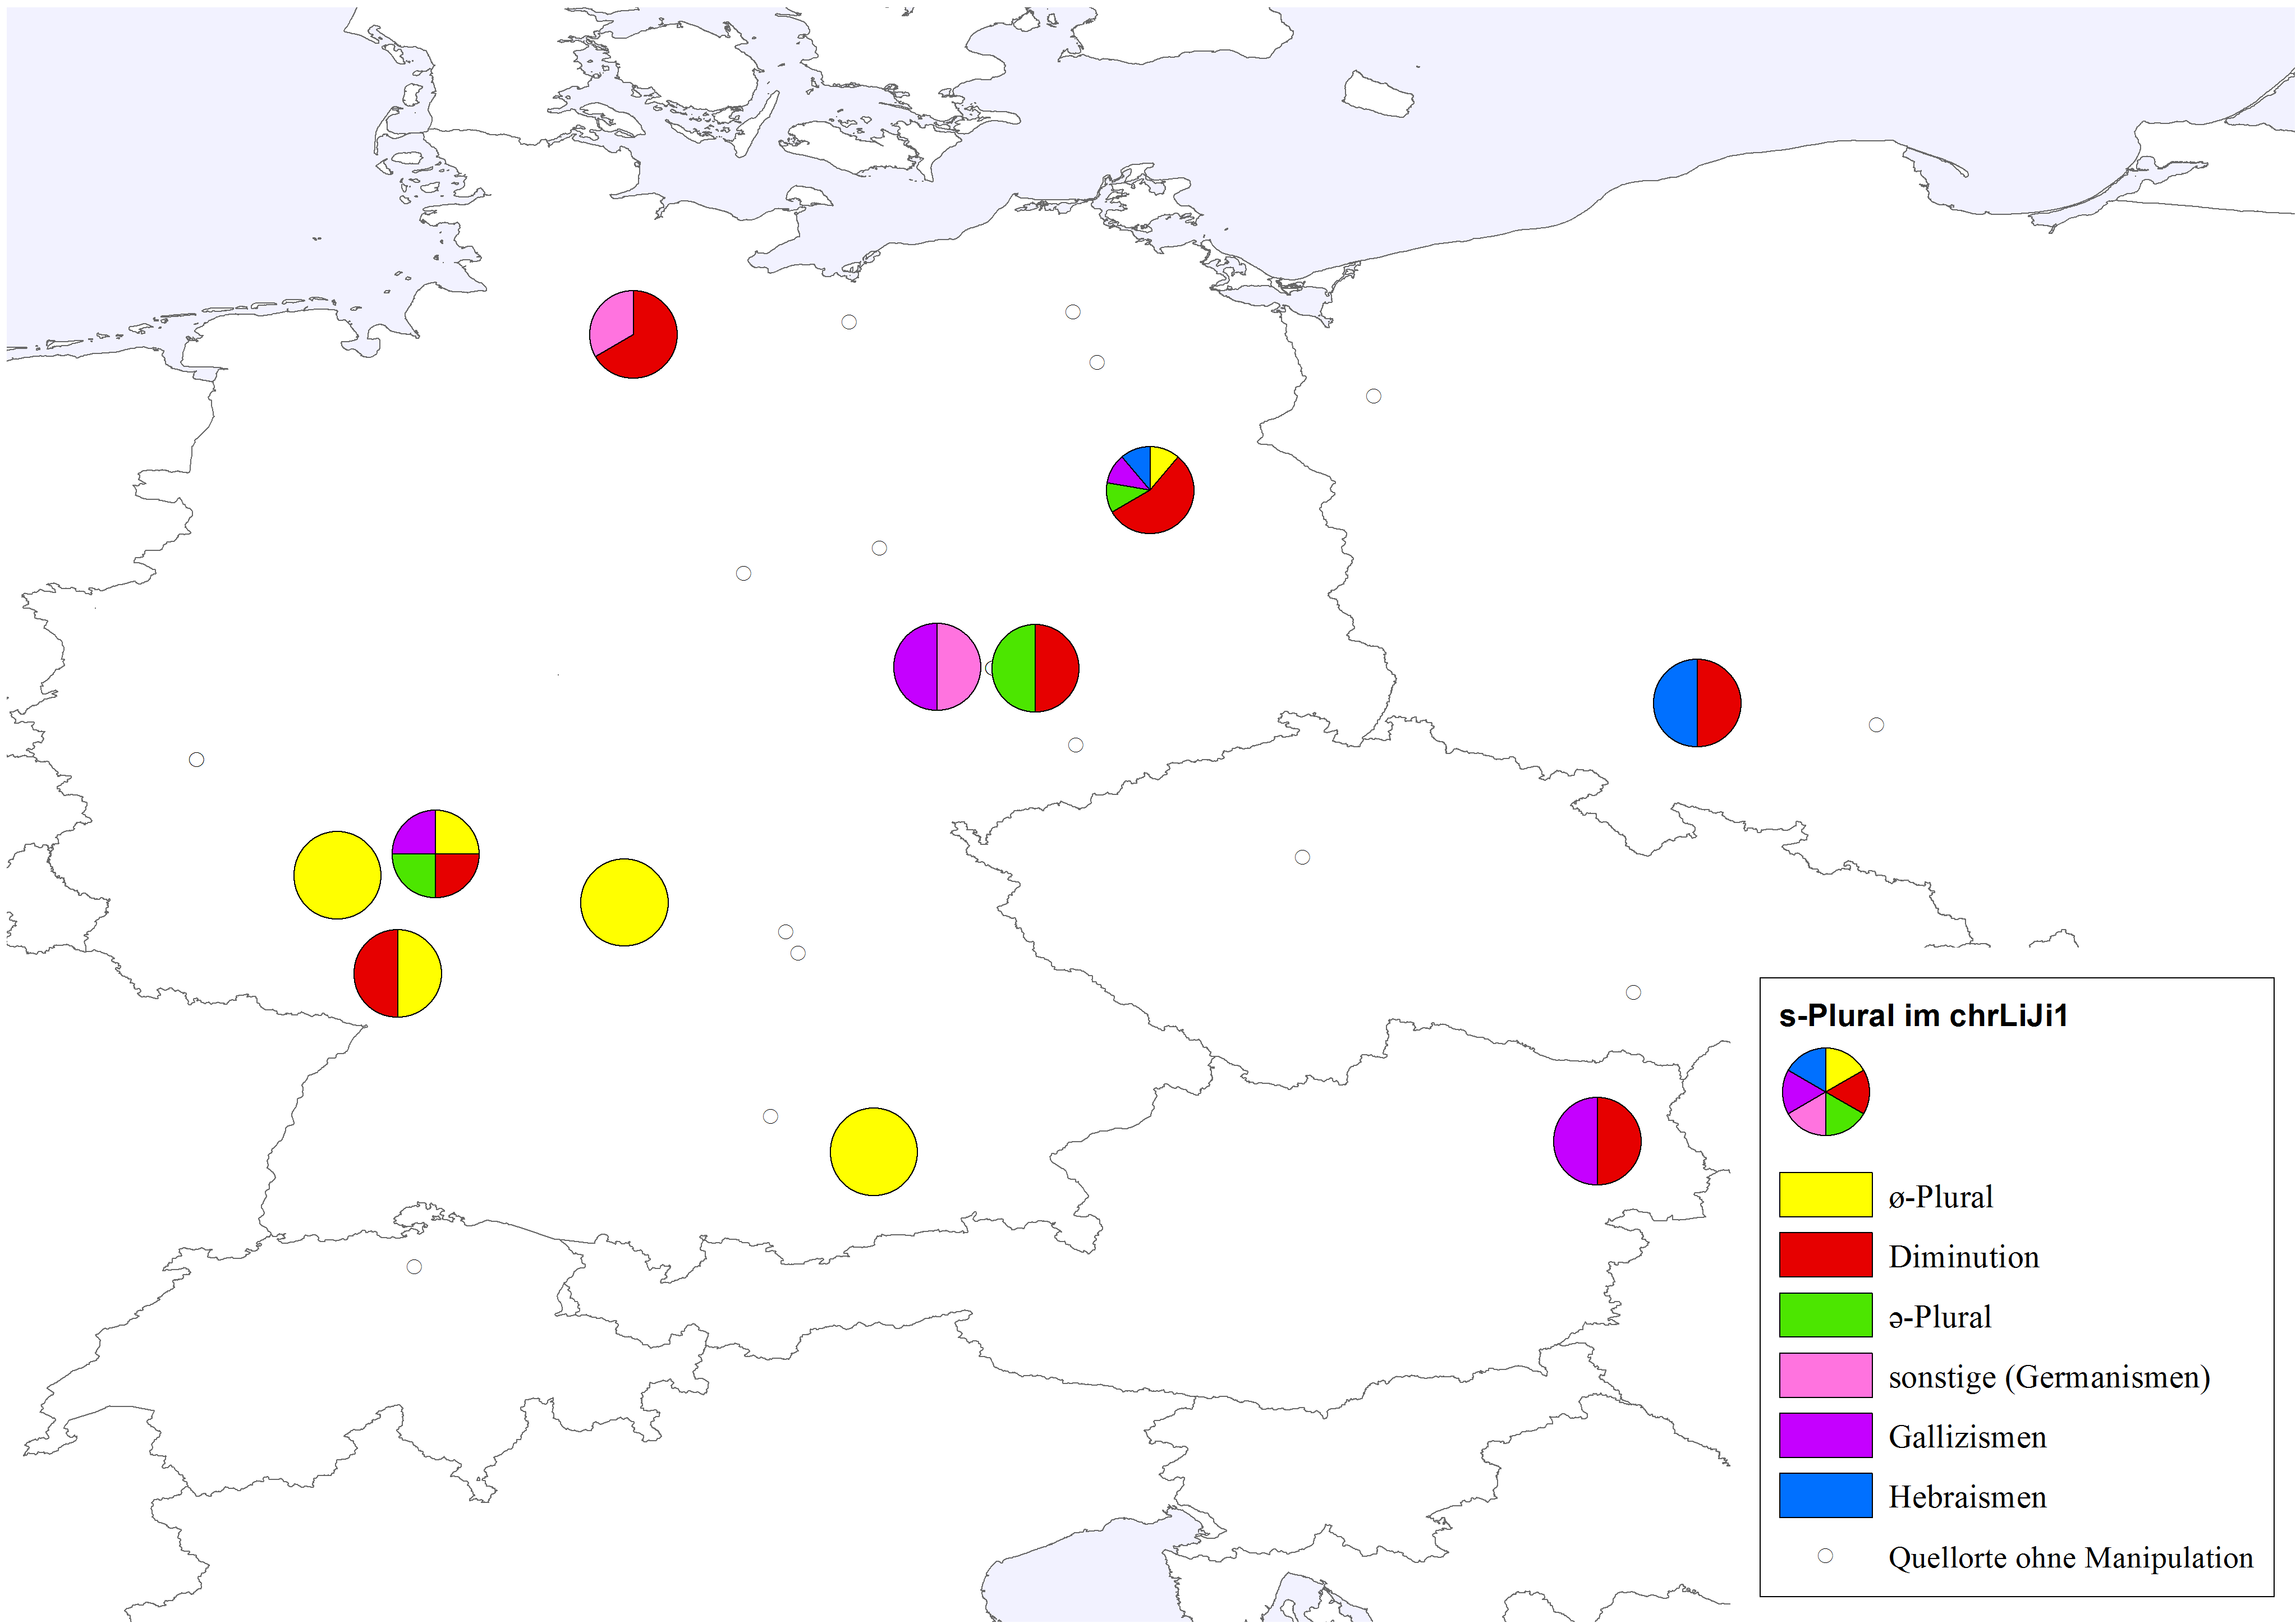
\includegraphics[scale=0.45]{figures/sPluralKUCHEN2.png}
		\caption{\label{sPluralKarte} \textit{s}-Plural im \hai{chrLiJi1}}
		\end{figure}
\FloatBarrier  %farbe des meeres neu / heller!!!
		
		
		   \begin{table}[h!]
%\centering
		\begin{tabularx}{\columnwidth}{XXc}

		\hline 
\textbf{Typen} & \textbf{Belege} [Pluralbildung im mod. \hai{OJ}]& \textbf{Quellen}   \\ \hline
\textbf{nhd. ∅-Plural}  &
\textit{Fischers} \sem{Fischer\textsubscript{Pl.}} (\hai{PG}:\,63) [oj. \RL{-ס}]; %\ili{OJ}
\textit{Feuerzettels} \sem{Feuerzettel\textsubscript{Pl.}} (\hai{NW}:\,9) [oj. \RL{-ען}]; \textit{Frackärmels} \sem{Frackärmel\textsubscript{Pl.}} (\hai{SV}:\,6) [oj. ∅-] \textit{Busens} \sem{Busen\textsubscript{Pl.}} (\hai{VD}:\,16) [oj. \RL{-ס}]; %\ili{OJ}  
& 4 \\


\textbf{alte Kollektiva (nhd. ∅-Plural)}  &
\textit{Gelärms} \sem{Gelärme\textsubscript{Pl.}} (\hai{FL}:\,38)\,[oj. –]; 
\textit{Gelafs} \sem{Gelaufe\textsubscript{Pl.}} (\hai{FL}:\,38) [oj. –];\textit{Ungewitters} \sem{Unwetter, Gewitter\textsubscript{Pl.}} (\hai{LM}:\,18)  [oj. –]; 
 & 2 \\

\textbf{\isi{Diminution}  (schriftl. nhd. ∅-Plural; oj. \RL{לעך}-, \RL{עלעך}-)}  & z.\,B. \textit{Blümches} \sem{Blume\textsubscript{Dim. Pl.}} (\hai{MV}:\,152), \textit{Baanches} \sem{Bein\textsubscript{Dim. Pl.}} (\hai{PG}:\,44), \textit{Gesellschaftges} \sem{Gesellschaft\textsubscript{Dim. Pl.}} (\hai{PA}:\,23),  \textit{Schicksels} \sem{Schickse\textsubscript{Dim. Pl.}, Nichtjüdin\textsubscript{Dim. Pl.}} (\hai{BP}:\,6; \hai{JP}:\,44), \textit{Gomolches} \sem{Kamel\textsubscript{Pl.}} (\hai{NW}:\,33) & 13 \\


\textbf{ə-Plural} & 
\textit{Kerls} \sem{Kerl\textsubscript{Pl.}} (\hai{VD}:\,18; \hai{AD}:\,138) [oj. –];  {Schnauzbarts} \sem{Schnauzbart\textsubscript{Pl.}} (\hai{AD}:\,139) [oj. ∅-]; \textit{Teppichs} \sem{Teppich\textsubscript{Pl.}} (\hai{NW}:\,8) [oj. \RL{-ער}]; 
 & 3\\  



\textbf{Hebraismen}  &
\textit{Gois} \sem{Nichtjude\textsubscript{Pl.}} (\hai{JK}:\,27) [oj. \RL{-ים}]
 & 1\\



\textbf{Gallizismen}  &
\textit{Dames} \sem{Damen\textsubscript{Pl.}} (\hai{NW}:\,71; \hai{PA}:\,5; \hai{TH}:\,135) [oj. \RL{-ן}\,\RL{-ס}]; %\ili{OJ}    
\textit{Cavalierers} \sem{Cavalier\textsubscript{Pl.}} (\hai{DW}:\,71) [oj. –] & 4\\



\textbf{Sonstige}  &
\textit{Herrens} \sem{Herr\textsubscript{Pl.}} (\hai{TH}:\,135) [oj. –]; 
\textit{Ette's} \sem{Vater\textsubscript{Pl.}} (\hai{JP}:\,44) [Lexem nicht im oj. vorhanden] & 2 \\ \hline

 \end{tabularx}
		 \caption{\textit{s}-Plurale im \hai{chrLiJi1}}
		 \label{tblsPLURAL}
		 \end{table}

 \FloatBarrier

Obwohl aus den authentischen Quellen des Westjiddischen keine auffällige Verwendung des Plural-\textit{s} bekannt ist, finden sich im \hai{jüdLiJi1} sehr wohl Belege, die denen des \hai{chrLiJi1} ähneln (vgl. Bsp. \ref{bspSjürliji1_1}–\ref{bspSjürliji1_8}). Unter den acht Belegen finden sich auch zwei Fälle, in denen ein \textit{s}-Plural dem ostjiddischen Standard entspräche (\ref{bspSjürliji1_3}, \ref{bspSjürliji1_4}). Besonders frequent sind auch hier \textit{s}-Plurale bei nhd. ∅-Plural (Bsp. \ref{bspSjürliji1_1}–\ref{bspSjürliji1_4}). Bei \textit{en}-Pluralen findet es sich gehäuft im Lexem \sem{Junge} in den \hai{GuS} (Bsp. \ref{bspSjürliji1_5}). Für Plural-\textit{s} an Stelle des Schriftdeutschen ə-Plurals gibt es nur einen Beleg im \hai{jüdLiJi1} (\ref{bspSjürliji1_8}). Besonders augenscheinlich an den Belegen für den \textit{s}-Plural im \hai{jüdLiJi1} ist, dass er ausschließlich in den Berliner Quellen, also umgeben vom niederdeutschen Substrat, auftritt, nicht aber in den Quellen aus dem ostmitteldeutschen bzw. ungarischen Raum. Da der \textit{s}-Plural im Niederdeutschen äußerst \isi{produktiv} ist (vgl. \cite[147–150]{Lindowetal1998}), liegt es nahe, diese Belege als Interferenz mit dem deutschen Dialekt zu deuten. 

 
Die Daten aus den drei Korpora deuten einen Rückgang an \textit{s}-Pluralen im \hai{LiJi} an. Die Funktion des \textit{s}-Plurals im Literaturjiddischen bleibt fragwürdig. Denkbar sind neben tatsächlichen Imitationen des (Ost-)Jiddischen auch Interferenzen mit den deutschen Dialekten. Zumindest im niederdeutschen Raum ist dies durchaus plausibel. Aber auch eine Markierung der Sprache als \quein{fremd} und besonders als \quein{mit-dem-Französischen-sympathisierend} kann mit Hilfe der \textit{s}-Plurale beabsichtigt sein. \\

\eenumsentence{
\item \textit{Italieniers} \sem{Italiener\textsubscript{Pl.}} (\hai{GuS1}:\,3); vgl. oj. ∅-\RL{איטא\makebox(-1.5,-7.5)[r]{\libertineGlyph{uni207B}}ליענער} \textit{italiener-∅} \label{bspSjürliji1_1}
\item \textit{Kellers} \sem{Keller\textsubscript{Pl.}} (\hai{GuS5}:\,4); vgl. oj. \RL{קעלער-ן} \textit{keler-n}\label{bspSjürliji1_2}
\item \textit{Schreibers} \sem{Schreiber\textsubscript{Pl.}} (\hai{PBerlin1}:\,4); vgl. oj. \RL{שר{יי}\makebox(-1.5,-7.5)[r]{\libertineGlyph{uni207B}}בער-ס} \textit{shrayber-s}\label{bspSjürliji1_3} %\ili{OJ}
\item \textit{Bergers} \sem{Bürger\textsubscript{Pl.}} (\hai{PBerlin2}:\,1.Sp., 2.Sp.); vgl. oj. \RL{בירגער-ס} \textit{birger-s}\label{bspSjürliji1_4} %\ili{OJ}


\item \textit{Jungens} \sem{Junge\textsubscript{Pl.}} (\hai{GuS10}:\,11; \hai{GuS15}:\,5; \hai{GuS23}:\,4); vgl. oj. \RL{ייִנגל-עך} \textit{jingl-ekh}\label{bspSjürliji1_5}


 \item \textit{Schtrümps} \sem{Strumpf\textsubscript{Pl.}} (\hai{PBerlin2}:\,1.Sp.); vgl. oj. \RL{שטריפ-∅} \textit{shtrimp-∅}\label{bspSjürliji1_8} 

}

 \FloatBarrier

\subsection{Der \textit{er}-Plural im \hai{LiJi}}\label{erPLURAL}
%  %\noindent
Neben dem starken Gebrauch von \textit{s}-Pluralen und Diminutivpluralen zeigt das \hai{LiJi} wenig Abweichungen vom Schriftdeutschen bei der Pluralbildung. Ein weiteres Phänomen deutet sich jedoch bereits im Rahmen der Pluraldiminution an (vgl. Unterabschnitt \ref{dimsg}). Eine häufige Strategie zur Bildung eines Pluraldiminutivums (im \hai{LiJi} wie auch in den dt. Dialekten) ist die Addition des Pluralmorphems \textit{-er} an ein Diminutivsuffix, z.\,B. in \textit{Stickelcher} \sem{Stück\textsubscript{Dim. Pl.}} (\hai{VD} Frankfurt, 1916:\,17, vgl. Tabelle \ref{tblDIMPL}). Der \textit{er}-Plural findet sich auch bei der normalen Pluralbildung in zwei Quellen des \hai{chrLiJi1} an schriftsprachlich untypischen Positionen (Bsp. \ref{bspERliji_1}--\ref{bspERliji_2}) und im \hai{jüdLiJi1} in zumindest einem Beleg (Bsp. \ref{bspERjüdliji}). Immerhin einer der drei Belege entspricht der Pluralbildung des modernen Ostjiddischen (\ref{bspERliji_2}). 

Aus \qu{Der Hochzeit zu Grobsdorf} kann eine besondere Verwendung dieses Pluralmorphems zumindest in Diminutiva (\ref{bspERgrob0}) und erstarrten Diminutiva (\ref{bspERgrob}) nachgewiesen werden. In Kontexten wie etwa (\ref{bspERliji_1}) findet es sich jedoch nicht (\ref{bspERgrob2}). 
Eine besondere Profilierung des \textit{er}-Plurals wäre vor allem im Mitteldeutschen und den koterritorialen jiddischen Varietäten anzunehmen. Der Beleg der fränkischen Quelle aus (\ref{bspERliji_1}) könnte somit unter Umständen tatsächlich auf eine Sprachrealität, wenn auch auf eine deutsch-dialektale, verweisen.\\


\eenumsentence{
\item \textit{Bahner} \sem{Bein\textsubscript{Pl.}} (\hai{GP} Nürnberg, 1831:\,28); vgl. oj. \RL{ביין-ער} \textit{beyn-er} \sem{Knochen} (vgl. Fn. \ref{fuss} S. \pageref{fuss})\label{bspERliji_1} %Nürnberg

\item \textit{Teppicher} \sem{Teppich\textsubscript{Pl.}} (\hai{AK} Zürich, 1948:\,224); vgl. oj. \RL{טעפּעך-ער} \textit{tepekh-er}\label{bspERliji_2}
%\ili{OJ}! vgl. AK hat auch n-Plural

\item \textit{Menscher} \sem{Mensch\textsubscript{Pl.}}(\hai{GuS5}:\,5);  vgl. oj. \RL{מענטש-ן} \textit{mentsh-n} \label{bspERjüdliji}

\item \RL{ווייבערכער} \textit{weibercher} \sem{Weib\textsubscript{Dim. Pl.}} (\qu{Die Hochzeit zu Grobsdorf} 1822:\,85)\label{bspERgrob0}

\item \RL{מערערכער} \textit{merercher} \sem{Mädchen\textsubscript{(Dim.) Pl.}} (\qu{Die Hochzeit zu Grobsdorf} 1822:\,70, 74, 90, 92, 95)  \label{bspERgrob}

\item \RL{בא\makebox(-1.5,-7.5)[r]{\libertineGlyph{uni207B}}ה} \textit{bah} \sem{Bein\textsubscript{Pl.}} (\qu{Die Hochzeit zu Grobsdorf} 1822:\,12)\footnote{Es handelt sich hier um einen ∅-Plural (keine \isi{Subtraktion}); vgl. \RL{בא\makebox(-1.5,-7.5)[r]{\libertineGlyph{uni207B}}ה} \textit{bah} \sem{Bein\textsubscript{Sg.}} (\qu{Die Hochzeit zu Grobsdorf} 1822:\,69).} \label{bspERgrob2}



}

%weiter

\subsection{Der \textit{en}-Plural im \hai{LiJi}}\label{enPLURAL}
%  %\noindent
Desweiteren finden sich in wenigen Quellen Belege für den \textit{en}-Plural, wo er im Schriftdeutschen nicht verwendet wird. So etwa in einer niederdeutschen Quelle (s. Bsp.\ref{bspENliji_1}), in der eine Interferenz mit dem deutschen Dialekt anzunehmen ist. Im \hai{chrLiJi1} finden sich wenige, einzelne Belege in vier Quellen (\ref{bspENliji_1}–\ref{bspENliji_5}); Im \hai{jüdLiJi1} (\ref{bspENjüliji1_1}) in einer Quelle. In \ref{BSPENPL} sind alle Belege für untypische \textit{en}-Plurale in den drei Korpora angeführt. Zum einen fällt dabei auf, dass dieses Suffix überwiegend an der Position von schriftsprachlich -ə (+ \isi{Umlaut}) steht (\ref{bspENliji_1}, \ref{bspENliji_5}). Die beiden übrigen Belege (\ref{bspENliji_3} u. \ref{bspENliji_4}) betreffen mit einem \isi{Hebraismus} ein \isi{Fremdwort}. Immerhin zwei der fünf Quellen des \hai{chrLiJi1}, die einen von der Schriftsprache abweichenden \textit{-(e)n} Plural in jüdischer Figurenrede verwenden, entsprechen damit der ostjiddischen Form (s. Bsp. \ref{bspENliji_1} u. \ref{bspENliji_5}), wenngleich ein niederdeutscher Einfluss im Beleg \ref{bspENliji_1} der Quelle \hai{UT} (Stavenhagen, 1862) nicht auszuschließen ist. Die Quelle \hai{AK} (Zürich, 1948), die bereits bei der Verwendung des ostjiddischen \textit{er}-Plurals aufgefallen ist (\ref{bspENliji_5}), zeigt auch hier die \quein{korrekte} oj. Pluralform (vgl. Bsp. \ref{bspERliji_2}, S. \pageref{bspERliji_2}).\\ 

 \eenumsentence{\label{BSPENPL}
 
\item \textit{Gerichten} \sem{Gericht\textsubscript{Pl.}} (\hai{UT} Stavenhagen, 1862:\,Kap. 3); vgl. oj. \RL{געריכט-ן} \textit{gericht-n}\label{bspENliji_1}

\item \textit{Goyen} \sem{Christ, Goy\textsubscript{Pl.}} (\hai{MS} Bonn, 1822:\,363L); vgl. oj. \RL{גוי-ם} \textit{goy-im} \label{bspENliji_3}

\item \textit{Schabbesgoien} \sem{Christ, Goy\textsubscript{Pl.}} (\hai{JK} Breslau, 1810:\,13); vgl. oj. s.\,o.\label{bspENliji_4}

 \item \textit{Kanaln} \sem{Kanal\textsubscript{Pl.}} (\hai{AK} Zürich, 1948:\,247); vgl. oj. \RL{קא\makebox(-1.5,-7.5)[r]{\libertineGlyph{uni207B}}נא\makebox(-1.5,-7.5)[r]{\libertineGlyph{uni207B}}ל-ן} \textit{kanal-n}\label{bspENliji_5}%\ili{OJ}


\item \textit{Tellern} \sem{Teller\textsubscript{Pl.}} (\hai{GuS23}:\,13); vgl. oj. \RL{טעלער-∅} \textit{teler-∅}\label{bspENjüliji1_1}

}


 
 \section{\isi{Flexion} von Eigennamen}\label{dativnamen}
 %\noindent
 Jiddisch flektiert den \isi{Dativ} und z.\,T. auch den \isi{Akkusativ} bei \isi{Eigennamen}, Familientermini und pränominale Genitive mittels der Suffigierung von -\textit{n} (\cite[161f]{Jacobs2005}; vgl. Bsp. \ref{dativOJ1}–\ref{dativOJ2}). \textcite[161]{Jacobs2005} spricht hier von einem obliquen Kasus. Seinen Ursprung haben diese Formen in der germanischen Komponente der schwachen \isi{Flexion} bei \isi{Eigennamen} des Alt- und Mittelhochdeutschen (vgl. \cite[insbes. 230f]{Nuebling2012}). Im Schriftdeutschen ging diese Eigennamenflexion, die durch Suffigierung von \textit{-e(n)} [± \isi{Umlaut}] erfolgte, im Verlauf des 19. Jahrhunderts vollständig verloren und wurde von Bildungen, die nun nur mehr den Plural vom Singular mittels \textit{-s}-Suffigierung markieren, abgelöst (z.\,B. \ref{BSPsNAME}, vgl. \cite[240]{Nuebling2012}).\footnote{In erstarrter Form erhalten blieb die alte \isi{Flexion} im Gegenwartsdeutsch – wohl aufgrund des Reimes – in der Phrase \textit{Futtern wie bei Muttern}.} In den hochdeutschen Mundarten blieben die alten Formen zum Teil konserviert. Bekannt ist dies etwa für die bairischen Mundarten Tirols (z.\,B. \ref{BSPDATIVTIROL}, vgl. \cite[50]{Schatz1903}). Defizitär, aber wesentlich vitaler ist die Eigennamenflexion mittels \textit{-e(n)} noch in friesischen und niederländischen Dialekten (\cite{Hoekstra2010}). Im Niederdeutschen ist die Eigennamenflexion jedoch nur mehr im pränominalen \isi{Genitiv} üblich (vgl. \cite[144]{Lindowetal1998}). 

 Im \hai{chrLiJi1} finden sich in zwei Quellen insgesamt drei Belege für die Eigennamenflexion an männlichen Vornamen (Bsp. \ref{dativ1}-\ref{dativ2.2}). Ein Beleg für die \isi{Flexion} eines weiblichen Vornamens tritt im \hai{jüdLiJi1} auf (Bsp. \ref{dativ3}). Dieses Phänomen ist damit generell kein äußerst frequentes Mittel zur Figurenmarkierung im \hai{LiJi}. Was es dennoch bemerkenswert macht, ist, dass es ausschließlich in nord-östlichen Quellen (Pyritz, Stavenhagen, Berlin), darunter die beiden niederdeutschen Quellen des \hai{chrLiJi1}-\isi{Korpus}, belegt ist. In Fritz Reuters \hai{UT} (Stavenhagen, 1862) findet sich die \isi{Flexion} von \isi{Eigennamen} auch im sprachlich unmarkierten Text, z.\,B. \ref{UTFRITZENNDT}. Man könnte nun annehmen, dass hier der ostjiddische Einfluss mitunter stärker gewirkt haben mag, als andernorts. Ein ostjiddischer Einfluss kann jedoch nicht die Erklärung für diese Belege liefern, da eine mögliche Sprache aus der diese Formen entlehnt sein können viel näher liegt: das Niederdeutsche selbst. \\
 


\eenumsentence{

\item \RL{רבֿקהן} \textit{rivken} \sem{Rebekka\textsubscript{Dat./Akk.}} (zitiert n. \cite[161]{Jacobs2005})\label{dativOJ1} 

\item \RL{באָבן} \textit{bobn} \sem{Großmutter\textsubscript{Dat./*Akk.}} (zitiert n. \cite[161]{Jacobs2005})\label{dativOJ2} 

 \item \textit{Die zwei Peters} \sem{Die zwei Peter\textsubscript{Pl.}} (vgl. \cite[240]{Nuebling2012})\label{BSPsNAME}
 
 \item \textit{i soks föttərn} \sem{ich sage es dem Vetter\textsubscript{Dat.}} (Ötztal, zitiert n. \cite[50]{Schatz1903})\label{BSPDATIVTIROL}
 
\item \textit{Würd Mosissen dat doch geling'n}\\
 \sem{würde Moses\textsubscript{Dat.} das doch gelingen} (\hai{DP} Pyrzyce, 1874:\,9)\label{dativ1} %Pyritz Sprache Niederdeutsch
 
 \item \textit{Rufen Sie Daviden} \sem{Rufen Sie David\textsubscript{Akk.}}(\hai{UT} Stavenhagen, 1862:\,Kap. 45) %Niederdeutsch
 
 \item \textit{\quein{Frau Pastorin}, säd Bräsig, \quein{mit Mosessen, das is woll 'ne bloße Erscheinung for Sie gewesen}} \\
 \sem{\quein{Frau Pastorin}, sagt Bräsig, \quein{das mit Moses\textsubscript{Dat.} ist wohl eine bloße Erscheinung für Sie gewesen.}} (\hai{UT} Stavenhagen, 1862:\,Kap. 45)\label{dativ2.2}%Niederdeutsch

 
  \item \textit{Grüße mir Riwken} \sem{Grüß mir Rebekka\textsubscript{Akk.}} (\hai{GuS1}:\,6)\label{dativ3} %jüd\ili{LiJi1} = Berlin
 
 
 \item \textit{Hawermann was desen Morgen mit Franzen nah Gürlitz tau Kirchen gahn} \\
 \sem{Hawermann war diesen Morgen mit Franz\textsubscript{Dat.} nach Gürlitz zur Kirche gegangen} (\hai{UT} Stavenhagen, 1862:\,Kap. 11)\label{UTFRITZENNDT}
 }
 
 \section{Kasussynkretismen}\label{kasus} 
%\noindent
 Das Kasussystem des modernen Ostjiddischen unterscheidet sich in vielfacher Weise vom Deutschen (vgl. \cite[154–222]{Jacobs2005}) und auch das Westjiddische zeigt einige dieser aus dem Ostjiddischen bekannten Strukturen (vgl. \cite{Fleischer2014}; \cite{FleischerSchaefer2012}; \cite[61–66]{Reershemius2007}).  So verwundert es kaum, dass auch im \hai{LiJi} Unterschiede gegenüber dem Schriftdeutschen im Bereich der Kasus zu finden sind.
  
\textcite[102]{Richter1995} stellt in den von ihm untersuchten Quellen des \hai{LiJi} den häufigen Gebrauch \qu{des Akkusativs anstelle des Dativs} fest. Er geht jedoch nicht näher auf die einzelnen Belege ein. Im \isi{Korpus} zum \hai{chrLiJi1} konnten Kasussynkretismen in drei Bereichen festgestellt werden: bei vollen Objekten in Nominalphrasen (Unterabschnitt \ref{kasusobj}), bei vollen Objekten in Präpositionalphrasen (Unterabschnitt \ref{kasuspräp}) und bei \isi{Pronomen} in Nominal- und Präpositionalphrasen (Unterabschnitt \ref{kasuspron}). Im Folgenden werden damit erstmals systematisch die Abweichungen des \hai{LiJi} vom Schriftdeutschen erfasst und mit den vorhandenen Daten zum West- und Ostjiddischen verglichen. \\


 
 \subsection{Kasus bei vollen Objekten}\label{kasusobj}
 %  %\noindent
Zum Kasussystem des Alt- oder Westjiddischen ist noch wenig Genaues bekannt. Die einzige Beschreibung eines westjiddischen Kasussystems, welches deutlich von der niederdeutschen Kontaktsprache gezeichnet ist, liefert bislang \textcite[61–66]{Reershemius2007}. Prinzipiell ist anzunehmen, dass sich \ili{Westjiddisch}  in einem ähnlichen Maß, wohl aber in unterschiedlichen Bereichen, vom Schriftdeutschen unterscheidet, wie das Ostjiddische. Da es an Vergleichsdaten fehlt, können lediglich die Situation im Ostjiddischen herangezogen  und die Belegdaten  aus den Korpora des \hai{LiJi} vorgestellt werden. 

 Das Standardjiddische  und -deutsche Kasussystem bei vollen Objekten\footnote{Darunter verstanden werden \hai{NP}s nach dem Muster \textit{\isi{Artikel} (+ \isi{Adjektiv}) + Nomen}.} unterscheidet sich in nur wenigen Punkten. Im Jiddischen ist der Genitivabbau weiter umgesetzt als im Schriftdeutschen, so dass man hier eher vom \quein{Possessiv} als vom \quein{Genitiv} spricht (\cite[110f]{Wolf1969}; \cite[172]{Jacobs2005}; \cite[403f]{Jacobsetal2013}). Im Singular entspricht die Form des Possessivs der des Dativs; im Plural hingegen des Akkusativs. Die zwei weiteren Unterschiede zum Deutschen sind die Synkretismen von Akk. Sg. m. mit Dat. Sg. m. zugunsten des Dativs und von Dat. Pl. mit Akk. Pl. zugunsten der Nominativ- bzw. Akkusativform. 
 
Das Kasussystem des Standardjiddischen entspricht weitestgehend dem der meisten jiddischen Dialekte (\cite[129]{Wolf1969}). Eine Ausnahme findet sich im \hai{SÜJ}, wo die Form des Dat. f. mit der des Akk. zusammengefallen ist (\cite[129]{Wolf1969}). Ein weitaus umfassenderer \isi{Synkretismus} fand im \hai{NOJ} statt, wo \isi{Akkusativ} und \isi{Dativ} zu einem obliquen Objektkasus (\qu{\RL{אָביעקט-בויגפא\makebox(-1.5,-7.5)[r]{\libertineGlyph{uni207B}}ל}}) zusammengefallen sind (\cite[160]{Zaretski1929}; \cite[117]{Wolf1969}).\label{FNKASUSDIALEKT} \\
 
  \begin{table}[h!]
%\begin{longtable}{ccc|ccc}
\centering
		\begin{tabular}{lllll}

		\hline 

\textbf{Quelle} &\textbf{Sg. m.} & \textbf{Sg. n.} & \textbf{Sg. f.} &\textbf{Pl.}  \\ \hline 

\hai{LS} & Nom. statt Akk. & –	& –	& Nom./Akk. statt Dat.\\

\hai{SS} & Dat. statt Akk. & –	& –	& –\\ 
 
\hai{AK} & Nom. statt Akk. & –	& –	& –\\ 
 
  \hline 
 \end{tabular}
		 \caption{Kasussynkretismen im \hai{chrLiJi1} bei vollen Objekten}
		 \label{tblOBJKASUS}
		 \end{table}
		% \end{longtable}

 
	Tabelle \ref{tblOBJKASUS} fasst alle Typen von Kasussynkretismen im \hai{chrLiJi1} zusammen. Eine Quelle (\ref{SS_DAT}) setzt tatsächlich den ostjiddischen \isi{Zusammenfall} im Sg. m. um und eine weitere (\ref{LS_PL}) zeigt den \isi{Synkretismus} von Akk. und Dat. im Plural. Daneben zeigt diese Quelle im Beleg (\ref{LS_NOM}) zumindest in einer Position Manipulationen, wo sich das Ostjiddische vom Schriftdeutschen unterscheidet (Sg. m. Akk.), wenn auch der ostjiddische \isi{Synkretismus} nicht den Nominativ betrifft. Hier ließe sich eine Hypernorm analog zum Plural (\ref{LS_PL}) annehmen. Für die Quelle \hai{AK} (Zürich, 1948) kann man von einer Interferenz mit dem Alemannischen ausgehen, wo sich der Nom.-Akk.-\isi{Synkretismus} durchgesetzt hat (vgl. \cite[665f]{Schirmunski1962}; s. Bsp. \ref{AK_NOM}).\\

\eenumsentence{
\item \textit{ich hob doch gekennt} [\textit{Ihrem Tate}]\textsubscript{Dat.} \textit{und Ihre Mammele} (\hai{SS} Berlin, 1907:\,9)\\
\sem{ich habe doch [Ihren Vater]\textsubscript{Akk.}  und Ihre Mutter gekannt}\label{SS_DAT}


\item \textit{Helf ich} [\textit{die Lait}]\textsubscript{Nom./Akk.} \textit{aus der Not} (\hai{LS} Bonn, 1925:\,13)\\
\sem{Helfe ich [den Leuten]\textsubscript{Dat.} aus der Not}\label{LS_PL}

\item \textit{und laß mer nicht nehme} [\textit{mei ehrlicher Name}]\textsubscript{Akk.} (\hai{LS} Bonn, 1925:\,4)\\
\sem{und lasse mir nicht [meinen ehrlichen Namen]\textsubscript{Dat.} nehmen}\label{LS_NOM}


\item \textit{Madam varstehn} [\textit{kein Spaß}]\textsubscript{Nom.}\textit{?}  (\hai{AK} Zürich, 1948:\,235)\\
\sem{Madam verstehen [keinen Spaß]\textsubscript{Akk.}?}\label{AK_NOM}

}


Für einen ostjiddischen Einfluss spricht besonders die diachrone Verteilung der Belege (s. Abb. \ref{histokasusNP}). Aber auch die geographische Lage der Quelle \hai{SS} (Berlin, 1907) spräche für einen möglichen Kontakt zum Ostjiddischen. Manipulationen des Kasus bei vollen Objekten sind beinahe ausschließlich in Quellen des 20. Jahrhunderts belegt. \\

  
 

\begin{figure}[h!]
	\begin{tikzpicture}
		\begin{axis}[only marks, width=0.82\textwidth,height=0.2\textheight,
		legend style={at={(1,1)},xshift=+0.2cm, yshift=-0.1cm,anchor=north west,nodes=left},
			xtick={1700, 1725, 1750, 1775, 1800, 1825, 1850, 1875, 1900, 1925, 1950, 1975}, ytick=\empty,
			x tick label style={/pgf/number format/1000 sep=}, 
			y tick label style={/pgf/number format/1000 sep=},
			extra y tick style={grid=major,
				tick label style={, ,}},
				ymin=0.7,
				ymax=3.5,
			ylabel={Phänomenbelege},
			enlarge x limits=0.03]	
	
\addplot [mark=square*, black] table [x=jahr, y=PL_NOM] {figures/KASUS_NP_PL_NOM.txt}; 			


\addplot [mark=square*, gray] table [x=jahr, y=SG_M_DAT] {figures/KASUS_NP_SG_M_DAT.txt}; 


\addplot [mark=*, gray] table [x=jahr, y=SG_M_NOM] {figures/KASUS_NP_SG_M_NOM.txt}; 



\addplot [mark=o,black] table [x=jahr, y=NO] {figures/KASUS_NP_NO.txt}; %1.5
 

						\legend{Akk. statt Dat. Pl., Nom. statt Akk. Sg.m., Dat. statt Akk. Sg.m., keine Manipulation} %macht Legende
		\end{axis}
	\end{tikzpicture}
	\caption{Diachrone Verteilung von Kasussynkretismen bei vollen Objekten im \hai{chrLiJi1}}
	\label{histokasusNP}	
\end{figure}
\FloatBarrier


 
 Doch auch ein deutsch-dialektaler Einfluss ist nicht auszuschließen. Den Daten \citeauthor{Shrier1965}s (\citeyear{Shrier1965}) zufolge können zumindest die Singularbelege auf koterritoriale Formen zurückgeführt werden: So findet sich der \isi{Zusammenfall} von \isi{Akkusativ} und Nominativ (beim Sg. m.) im gesamten Südwesten (Alemannisch, Mosel- u. Rheinfränkisch und z.\,T. im Brandenburgischen) (\cite[423f]{Shrier1965}). Die zwei Quellen des \hai{chrLiJi1}, die diesen \isi{Synkretismus} zeigen, stammen aus Zürich und Bonn, also eben jenen Regionen. Der \isi{Zusammenfall} von \isi{Akkusativ} und \isi{Dativ} (beim Sg. m.) findet sich hingegen besonders im Ostmitteldeutschen, im gesamten Niederdeutschen und in Teilen des Mittel- und Südbairischen (\cite[423f]{Shrier1965}). Die Quelle, die diesen \isi{Synkretismus} aufweist, stammt aus Berlin und damit wiederum aus eben jenem Gebiet, in dem der Akkusativ-Dativ-\isi{Synkretismus} auch bei den Pronomina recht prominent ist. Wenn auch sicherlich nicht beabsichtigt, so mag unterschwellig die eigene Dialekt- bzw. Regiolektkompetenz der einzelnen Autoren in die Imitationen hinein gespielt haben. \\
 

Abschließend lässt sich festhalten, dass Kasusmarkierungen am vollen Objekt im \hai{LiJi} ein eher peripheres Phänomen darstellen. In wenigen Fällen konnten Synkretismen, die aus dem Ostjiddischen bekannt sind, nachgewiesen werden. Die sich mittlerweile andeutende Tendenz des \hai{LiJi}, sich morphosyntaktisch stärker als etwa phonologisch am Ostjiddischen zu orientieren, könnte sich auch hier bestätigt sehen. Um die Situation jedoch sicher bewerten zu können, fehlt es an Daten zu den (west-)jiddischen Dialekten. \\
 
 
  \subsection{Kasus nach Präposition}\label{kasuspräp}
  %  %\noindent
  
Im Deutschen regieren Präpositionen die Kasuszuweisung. Dabei hängt diese von den semantischen Bedingungen (statisch vs. direktional) ab (\cite[23]{PittnerBerman2007}). So fordern Präpositionen in direktionaler \isi{Semantik} den \isi{Akkusativ} (\ref{BSPAKKDIREKTIONAL}); in statischer \isi{Semantik} jedoch den \isi{Dativ} (\ref{BSPDATSTATISCH}). Im modernen Jiddischen hingegen spielt die \isi{Semantik} keinerlei Rolle. Auf eine Präposition folgt immer der \isi{Dativ} (\ref{BSPJIDDIREKT}–\ref{BSPJIDSTAT}) (\cite[202]{Jacobs2005}; \cite{FleischerSchaefer2012}). Das ostjiddische Muster vom \isi{Dativ} als \quein{Einheitskasus} nach \isi{Präposition} findet sich ebenso im Süd- und Zentralwestjiddischen (z.\,B. in \ref{BspDATGROBS}; \cite{FleischerSchaefer2012}; \cite[24]{GuggenheimGruenberg1966}) und kann als eines der Indizien für die gemeinsame Genese von Ost- und \ili{Westjiddisch} gelten (\cite{Fleischer2014}).\\
 
 
 \eenumsentence{


 \item dt. \textit{er geht in die Stadt}\textsubscript{lokal-direktional}\label{BSPDATSTATISCH}
 
  \item dt. \textit{er wohnt in der Stadt}\textsubscript{lokal-statisch}\label{BSPAKKDIREKTIONAL}
 
 
   \item mod. \ili{Ostjiddisch} \textit{er geyt in der shtot}\textsubscript{lokal-direktional}\label{BSPJIDDIREKT}
   
 
  \item mod. \ili{Ostjiddisch} \textit{er voynt in der shtot}\textsubscript{lokal-statisch}\label{BSPJIDSTAT}

  
  \item \RL{איץ ווא\makebox(-1.5,-7.5)[r]{\libertineGlyph{uni207B}}רד אופפעם דא\makebox(-1.5,-7.5)[r]{\libertineGlyph{uni207B}}נץ געמא\makebox(-1.5,-7.5)[r]{\libertineGlyph{uni207B}}רשירט} \\
  \textit{iz ward uffem danz gemarschirt}\textsubscript{lokal-direktional} \\
  \sem{Jetzt wird auf den (wörtl. dem) Tanz marschiert}\\
  (\qu{Die Hochzeit zu Grobsdorf} 1822:\,53) \label{BspDATGROBS}
  
  
  \begin{flushright}
  (Bsp. \ref{BSPDATSTATISCH}–\ref{BSPJIDSTAT} zitiert n. \cite[415]{FleischerSchaefer2012}; \\
  Bsp. \ref{BspDATGROBS} vgl. \cite[423]{FleischerSchaefer2012})
    \end{flushright}
 
 
 }
 
 Im Plural sind \isi{Akkusativ} und \isi{Dativ} in Ost- und \ili{Westjiddisch} in die Akkusativform zusammengefallen (vgl. Unterabschnitt \ref{kasusobj} S. \pageref{kasusobj}). Dies spiegelt sich auch im Kasus nach \isi{Präposition} wider (\cite{FleischerSchaefer2012}). Im Plural ist daher von einer jiddischen Varietät der \isi{Akkusativ} an Stelle des Dativs zu erwarten. Im \hai{NOJ}, wo \isi{Dativ} und \isi{Akkusativ} generell zusammengefallen sind (s.\,o. S. \pageref{FNKASUSDIALEKT}; \cite[160]{Zaretski1929}), verhalten sich hingegen Singular und Plural identisch. Das Jiddische Nordpolens (\cite{Herzog1965}) und das nordöstliche \ili{Westjiddisch} zeigen ein zum standardostjiddischen komplementäres System (\cite{FleischerSchaefer2012}; \cite[130–132]{Herzog1965}). Hier  ist der Einheitskasus nach \isi{Präposition} der \isi{Akkusativ}, nicht der \isi{Dativ}. Ob und wie weit diese Form ins östliche \hai{ZWJ}, \hai{SWJ} bzw. \hai{SÜJ} hineinstreut, konnte aufgrund der dünnen Quellenlage noch nicht geklärt werden. \textcite{FleischerSchaefer2012} finden jedoch Anhaltspunkte, dass der \isi{Akkusativ} nach \isi{Präposition} ggf. auch in den dortigen jiddischen Varietäten verbreitet war. Entsprechende Daten, wie sich die deutschen Mundarten flächendeckend beim Kasus nach \isi{Präposition} verhalten, liegen bislang keine vor. 
 
Die Analyse des \hai{LiJi} kann nur Verstöße gegen das deutsche Schriftsystem erfassen, also nur die Fälle, in denen der \isi{Dativ} an der Position von deutsch \isi{Akkusativ} erscheint bzw. der umgekehrte Fall eintritt. Hier werden zunächst nur volle \hai{NP}s nach \isi{Präposition} behandelt. Darauf, wie sich \isi{Pronomen} nach Präpositionen im \hai{LiJi} verhalten, wird in Abschnitt \ref{kasuspron} näher eingegangen. Die Tabellen \ref{tblpräpkasus1} und \ref{tblpräpkasusjüdliji}  
geben die Belege dieser Verstöße an. 23 Quellen (43\%) des \hai{chrLiJi1} und 8 (von 10) Quellen des \hai{jüdLiJi1} 
zeigen solcherlei \quein{Verstöße}. 

Besonders auffällig ist, dass im Plural in allen drei Korpora vielfach und beinahe ausschließlich der \isi{Akkusativ} als Markierung eingesetzt wird. Der \isi{Akkusativ} im Plural findet sich in 13 Quellen des \hai{chrLiJi1} und in drei Quellen des \hai{jüdLiJi1}.  
Lediglich zwei Quellen des \hai{chrLiJi1} (\hai{PP} Berlin, 1839 u. \hai{WA}) setzen den \isi{Dativ} an Stelle des Akkusativs im Plural. Das heißt, dass sich das \hai{LiJi} zumindest im Plural deutlich am jiddischen System orientiert und dieses korrekt umsetzt. Belege für den \isi{Akkusativ} im Plural finden sich im gesamten Untersuchungsgebiet (vgl. Abb. \ref{kartepaepPL}). Areal auffällig verhalten sich die zwei Belege für den \isi{Dativ} im Plural. Deren Vorkommen im Nordosten kann jedoch auch ein rein zufälliges Raumbild sein.

Im Singular tritt die jiddische Verwendung des Dativs nur selten hervor. Im \hai{chrLiJi1} finden sich hierfür lediglich drei Belege im Femininum, zwei im Neutrum und ein Beleg im Maskulinum. Das \hai{jüdLiJi1} hingegen zeigt in keiner einzigen Quelle diese Form.

An Stelle einer Markierung jüdischer Figuren über den \isi{Dativ} nach \isi{Präposition} findet sich in einer deutlichen Vielzahl der Quellen der \isi{Akkusativ} statt des Dativs nach \isi{Präposition} mit lokal-statischer \isi{Semantik}. Wir finden dies in allen drei Korpora. Im \hai{chrLiJi1} findet sich der \isi{Akkusativ} nach \isi{Präposition} an Stelle des Dativs in einer Quelle im Maskulinum, in zehn im Neutrum und in elf im Femininum. Im \hai{jüdLiJi1} ist eine ähnliche Verteilung auf die drei Genera gegeben: zwei Quellen verwenden den \isi{Akkusativ} an der Position des Dativs im Maskulinum, fünf im Neutrum und fünf im Femininum. Den \isi{Akkusativ} als Einheitskasus nach \isi{Präposition} finden wir besonders im nordöstlichen \ili{Westjiddisch} und im Ostjiddischen Nordpolens (s.\,o.). Für das \hai{jüdLiJi1}, dessen Quellen aus genau dieser Region des Akkusativs als Einheitskasus nach \isi{Präposition} stammen, hieße dies, dass hier eine tatsächliche Sprachrealität wiedergegeben wird. 

Die areale Staffelung der Belege für den Singular zeigt ein interessantes Bild (Abb. \ref{kartepaepSG}): Die deutliche Mehrzahl der (wenigen) Belege für den \isi{Dativ} nach Präpositionen mit lokal-direktionaler \isi{Semantik} finden sich im Rhein-Main-Gebiet und damit im Gebiet des westlichen Westjiddischen, in welchem diese Form zu erwarten wäre (vgl. \cite{FleischerSchaefer2012}). Ein weiterer Beleg stammt aus Berlin, wo hingegen ein ostjiddischer Einfluss plausibel wäre. Die Quellen, in denen \isi{Akkusativ} an Stelle vom schriftdeutschen \isi{Dativ} steht, finden sich besonders im Osten des Erhebungsgebiets. \hai{chrLiJi1} liefert hiermit weitere Hinweise für die Annahme, dass dieser \isi{Akkusativ} weiter in den Südosten hinein streut als bislang angenommen (vgl. \cite{FleischerSchaefer2012}). Allerdings finden sich auch einige Belege für den \isi{Akkusativ} im äußersten Westen, was wiederum gegen die areale Relevanz des Datenmaterials spricht.

Die diachrone Verteilung der Belege des \hai{chrLiJi1} zeigt ein auffälliges Bild (s. Abb. \ref{histokasusPP}): Markierungen am Kasus nach \isi{Präposition} treten, von wenigen Ausreißern abgesehen, ab den 1820er Jahren auf und finden sich ab diesem Zeitpunkt in beinahe jeder Quelle. Dabei sind Belege für den \isi{Dativ} im Singular, also die standardostjiddische und west-westjiddische Form eher in den Quellen des 20. Jahrhunderts anzutreffen. Hingegen tritt der \isi{Akkusativ} als Einheitskasus bereits in den frühesten Belegen (1778, 1802) einer Manipulation des Kasus nach \isi{Präposition} auf.\\


	
\begin{figure}[h!]
	\begin{tikzpicture}
		\begin{axis}[only marks, width=0.82\textwidth,height=0.2\textheight,
		legend style={at={(1,1)},xshift=+0.2cm, yshift=-0.0cm,anchor=north west,nodes=left},
			%title={Funktionstypen des sp\"aten Westjiddisch},
			xtick={1700, 1725, 1750, 1775, 1800, 1825, 1850, 1875, 1900, 1925, 1950, 1975}, ytick=\empty,
			x tick label style={/pgf/number format/1000 sep=}, 
			y tick label style={/pgf/number format/1000 sep=},
			%extra y ticks={456.1, 1022.4},
			%extra y tick labels={{456,1},{1022,4}},
			extra y tick style={grid=major,
				tick label style={, ,}},
				ymin=0.7,
				ymax=6.3,
			ylabel={Phänomenbelege},
			enlarge x limits=0.03]	

\addplot [mark=square*, black] table [x=jahr, y=PL_DAT] {figures/Kasus_Pron_PL_DAT.txt}; 	
	
\addplot [mark=square*, gray] table [x=jahr, y=PL_AKK] {figures/Kasus_Pron_PL_AKK.txt}; 			


\addplot [mark=*, black] table [x=jahr, y=DAT_statt_AKK] {figures/Kasus_Pron_DAT_statt_AKK.txt}; 


\addplot [mark=*, gray] table [x=jahr, y=AKK_statt_DAT] {figures/Kasus_Pron_AKK_statt_DAT.txt}; 



\addplot [mark=o,black] table [x=jahr, y=NO] {figures/Kasus_Pron_NO.txt}; %1.5
 

						\legend{Dat. statt Akk. Pl., Akk. statt Dat. Pl., Dat. satt Akk. Sg., Akk. statt Dat. Sg., keine Manipulation} %macht Legende
		\end{axis}
	\end{tikzpicture}
	\caption{Verstöße gegen das schriftdeutsche Kasussystem im \hai{chrLiJi1} bei Präpositionalphrasen}
	\label{histokasusPP}	
\end{figure}
\FloatBarrier


 
 \begin{table}[h!]

\centering
		\begin{tabular}{lllll}

		\hline 

\textbf{Quelle} &\textbf{Sg. m.} & \textbf{Sg. n.} & \textbf{Sg. f.} &\textbf{Pl.}  \\ \hline 

\hai{PP} &	–	  &	–	& –	&  Akk. $>$ Dat.	\\
\hai{BW} &	–	  &	Dat. $>$ Akk.	& –	& –	\\
\hai{LM} &	–	  &	–	&	Akk. $>$ Dat. & –	\\
\hai{BP} &	–	  &	Dat. $>$ Akk.	& –	& Dat. $>$ Akk.\\
\hai{GP} &	–	  &	–	& Dat. $>$ Akk.	& Dat. $>$ Akk.	\\
\hai{PG} &	–	  &	–	&	Dat. $>$ Akk.; Akk. $>$ Dat. & Dat. $>$ Akk. 	\\
\hai{TH} &	–	  &	–	&	Dat. $>$ Akk. & Dat. $>$ Akk. 	\\
\hai{AJ} &	–	  &	Dat. $>$ Akk.	&	Dat. $>$ Akk.& Dat. $>$ Akk.	\\
\hai{MS} &	–	  &	–	& –	& Akk.	\\
\hai{PA} &	–	  &	–	& Dat. $>$ Akk.	& –	\\
\hai{WA} &	–	  &	Dat. $>$ Akk.	&	Dat. $>$ Akk. &  Dat. $>$ Akk.; Akk. $>$ Dat.	\\
\hai{UT} (ndt.)&	–	  &	Dat. $>$ Akk.	& –	& 	Dat. $>$ Akk.\\
\hai{AB} &	–	  &		Dat. $>$ Akk.& –	& –	\\
\hai{JP} &	–	  &	Dat. $>$ Akk.	&	Dat. $>$ Akk.& –	\\
\hai{SS} &		Akk. $>$ Dat.  &	–	& –	& –	\\
\hai{FL} &	–	  &	–	&Dat. $>$ Akk.	& Dat. $>$ Akk.	\\
\hai{VD} &	–	  &		Akk. $>$ Dat. &	Akk. $>$ Dat. & Dat. $>$ Akk.	\\
\hai{AD} &	–	  &	–	&	Dat. $>$ Akk.& Dat. $>$ Akk.	\\
\hai{MV} &	–	  &Dat. $>$ Akk.&Dat. $>$ Akk.	& –	\\
 \hai{DG} &	–	  &	–	&	Dat. $>$ Akk.& Dat. $>$ Akk.	\\
\hai{GW} &	–	  &	Akk. $>$ Dat.	& –	& –	\\
 \hai{SV} &	–	  &	Dat. $>$ Akk.	& –	& –	\\
 \hai{AK} &	Dat. $>$ Akk.  &	Dat. $>$ Akk.	& –	& Dat. $>$ Akk.	\\

 
  \hline 
 \end{tabular}
		 \caption{Diachrone Verteilung von Verstößen gegen das schriftdeutsche Kasussystem im \hai{chrLiJi1} bei Präpositionalphrasen}
		 \label{tblpräpkasus1}
		 \end{table}

	
	
	

	
	
	
	\begin{figure}[h!]
\centering
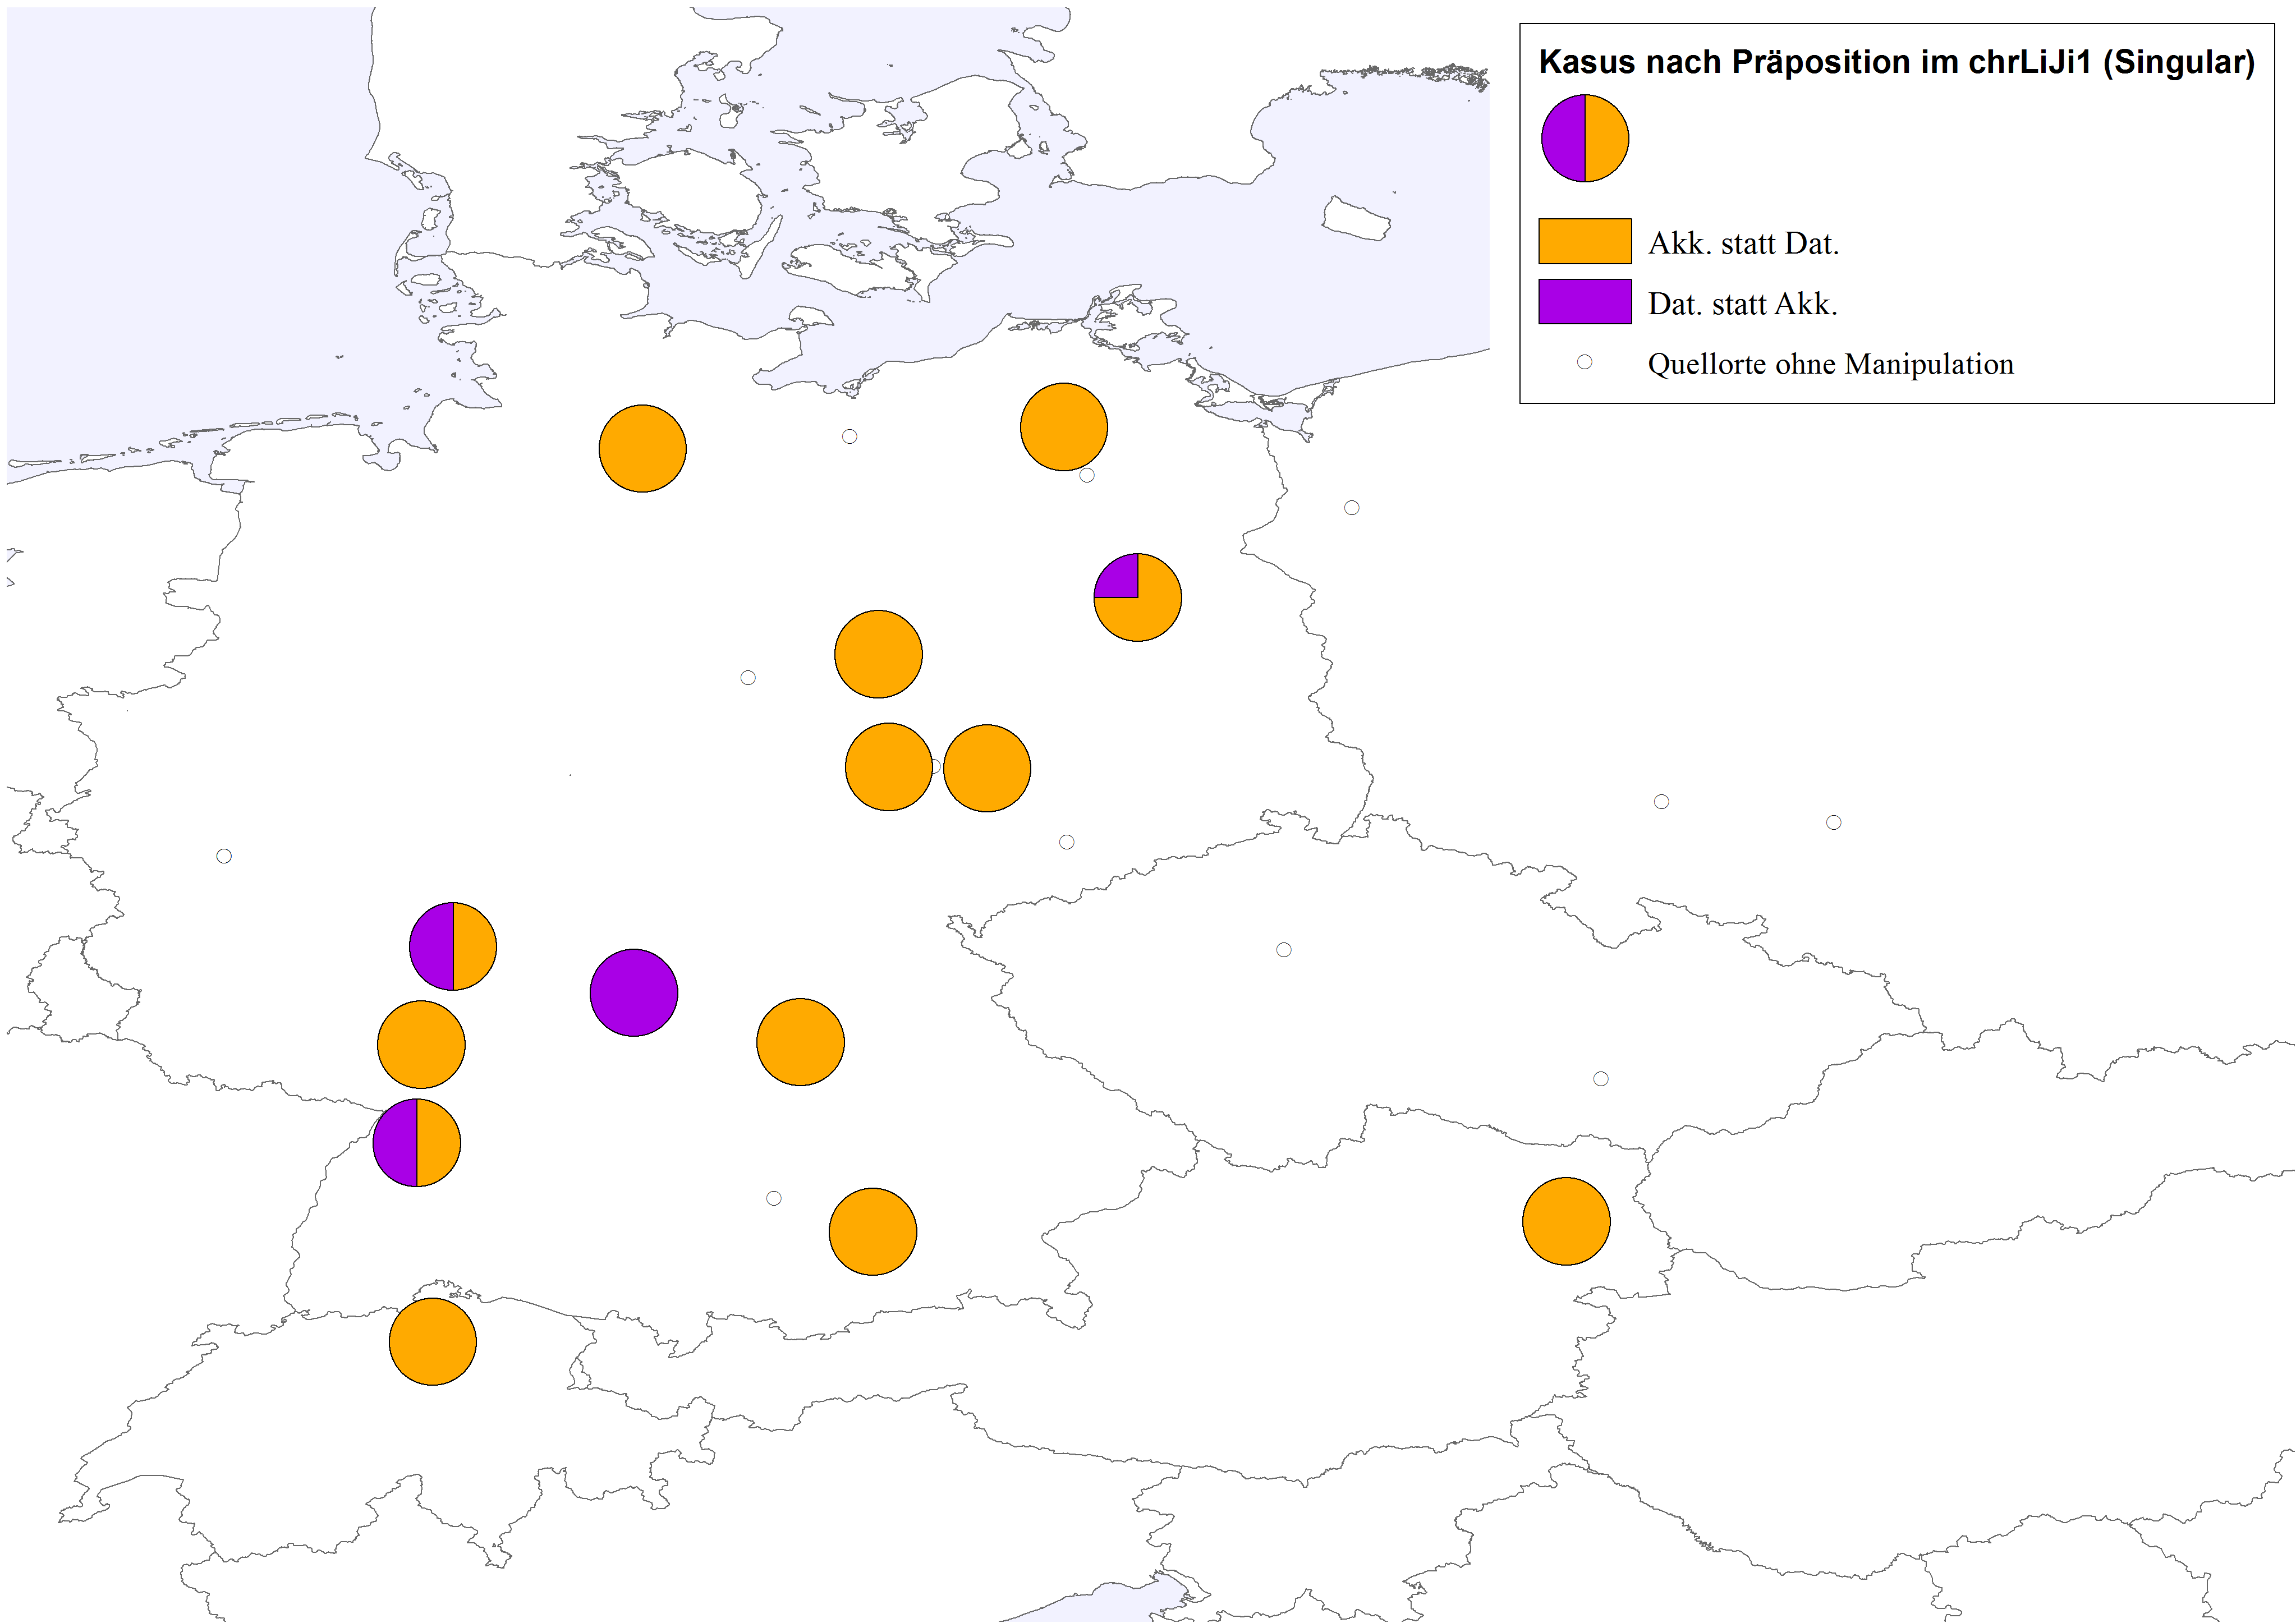
\includegraphics[scale=0.4]{KARTE_KASUS_PAEP_SG.png}
		\caption{\label{kartepaepSG} Kasus nach \isi{Präposition} im \hai{chrLiJi1} (Singular)}
		\end{figure}  


\begin{figure}[h!]
\centering
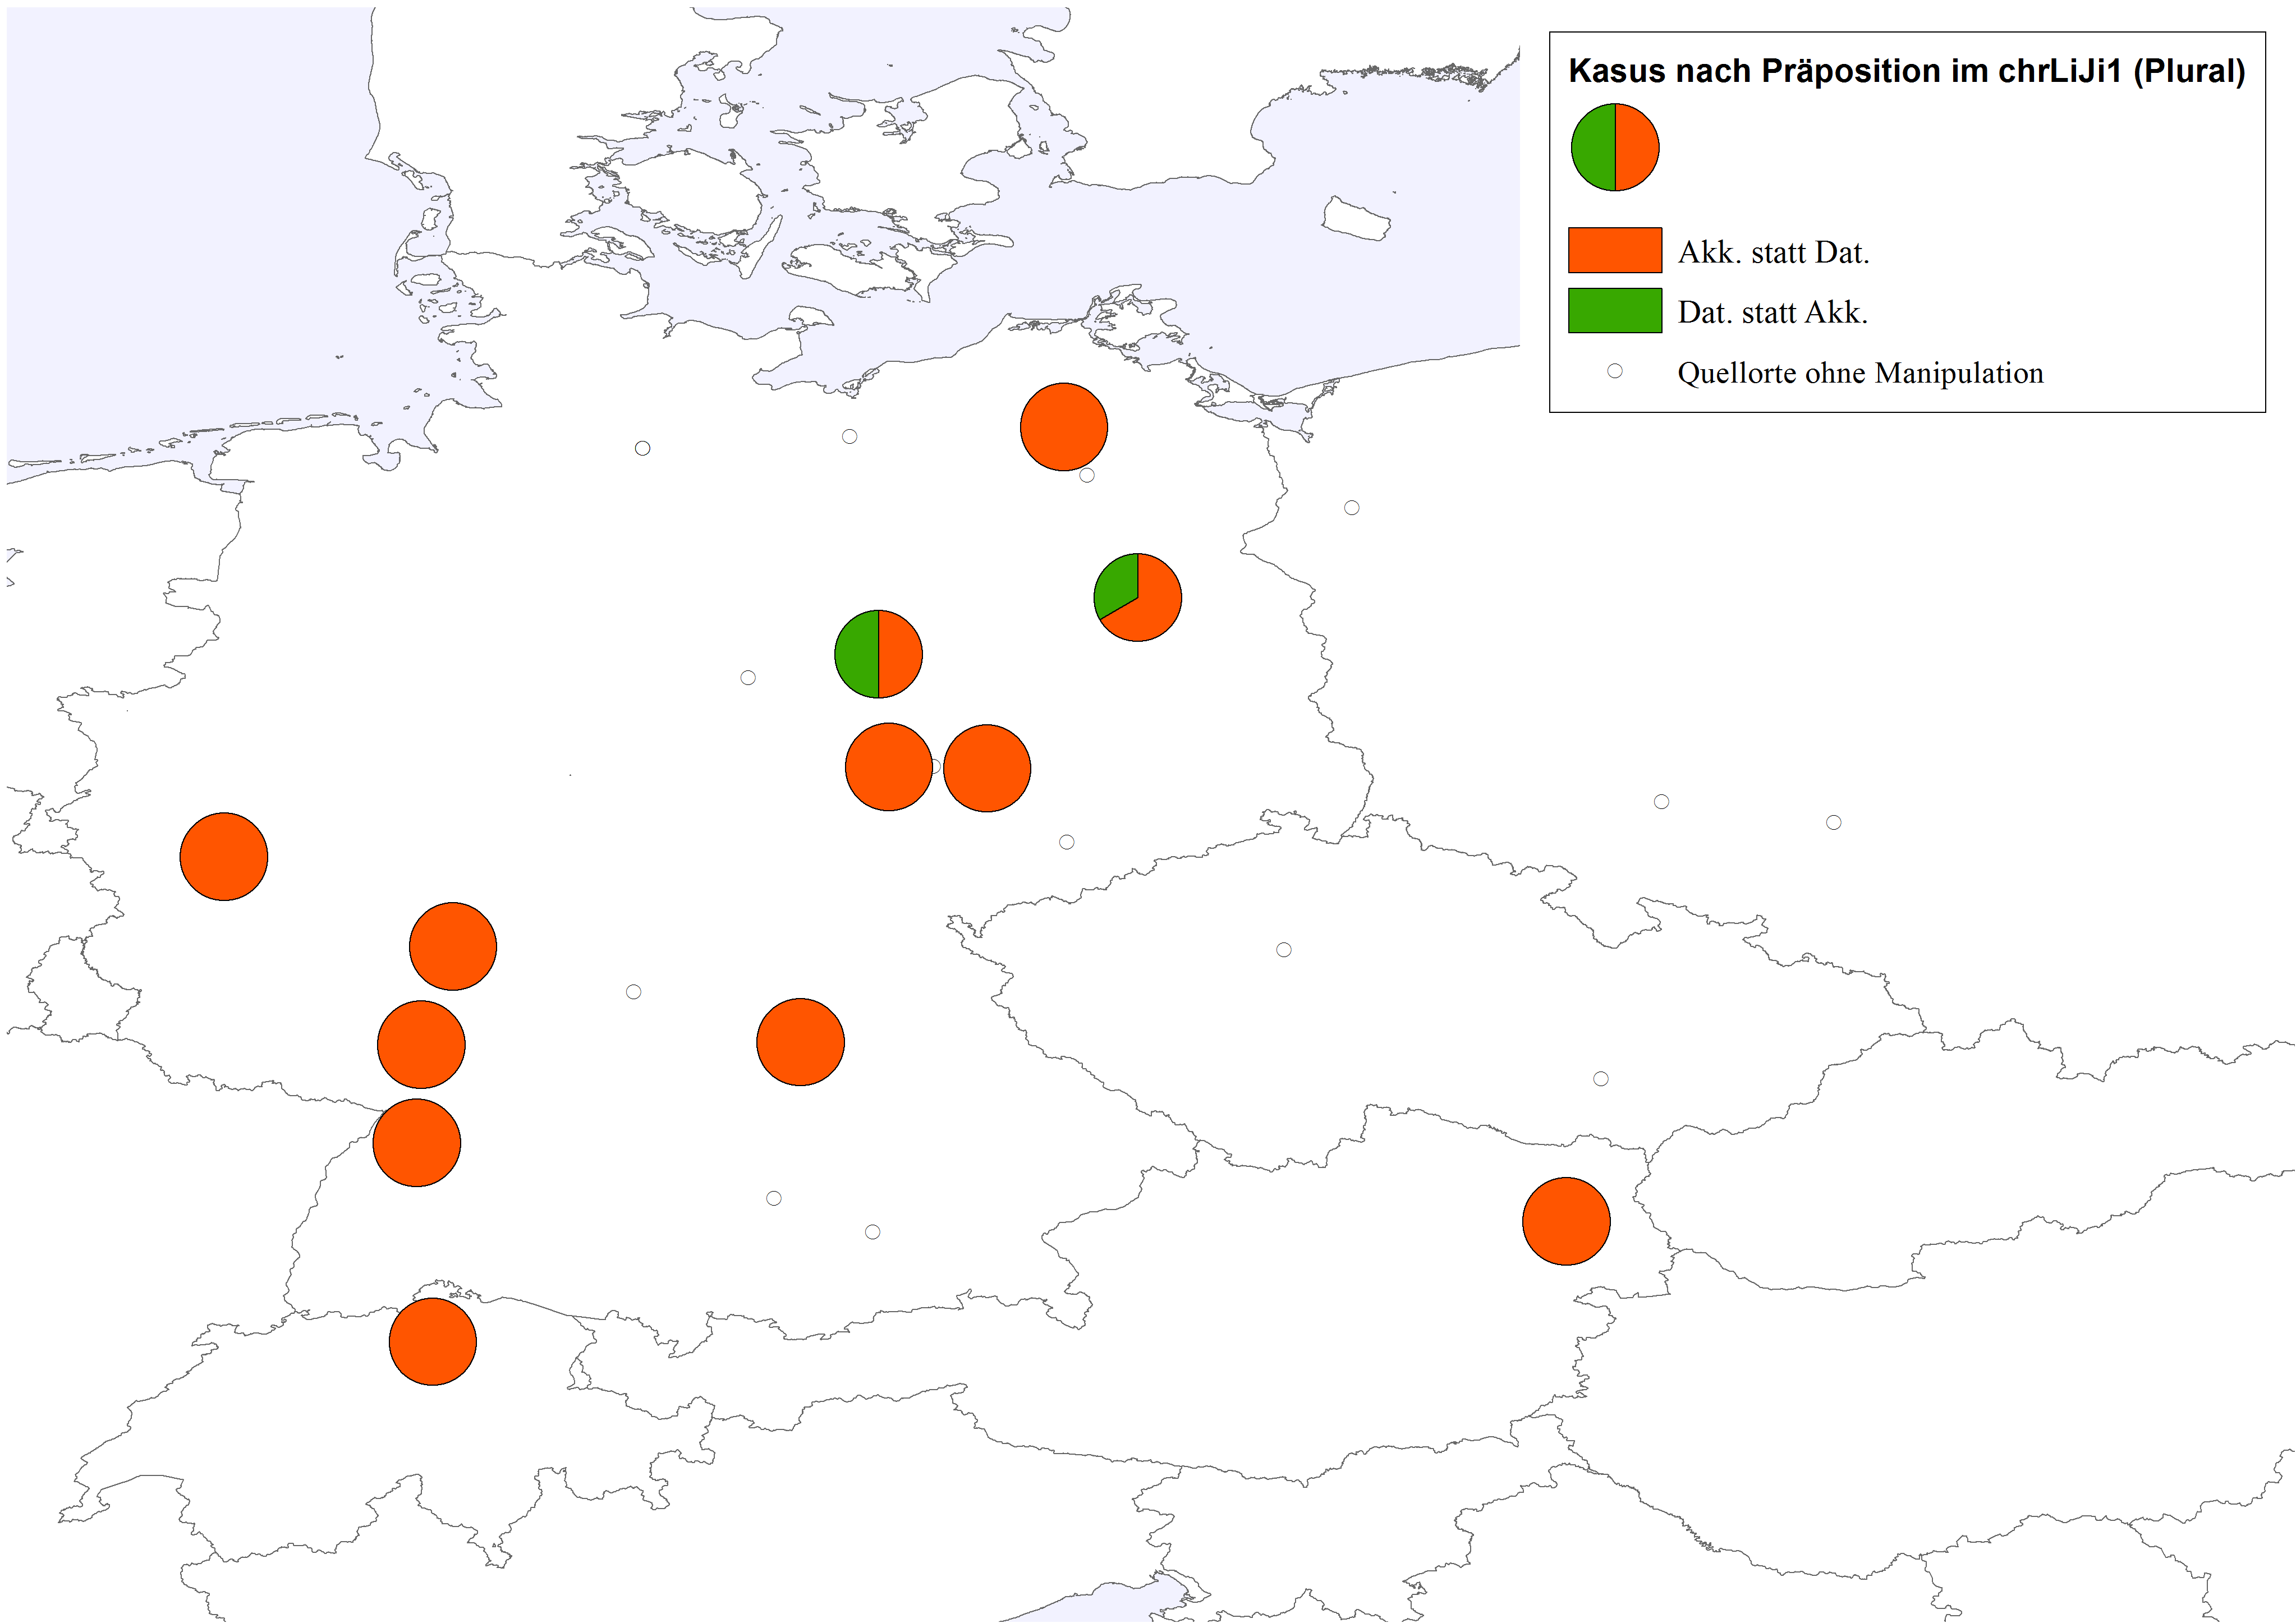
\includegraphics[scale=0.4]{KARTE_KASUS_PAEP_PL.png}
		\caption{\label{kartepaepPL} Kasus nach \isi{Präposition} im \hai{chrLiJi1} (Plural)}
		\end{figure}
\FloatBarrier

	
	
	 \begin{table}[h!]

\centering
		\begin{tabular}{lllll}

		\hline 

\textbf{Quelle} &\textbf{Sg. m.} & \textbf{Sg. n.} & \textbf{Sg. f.} &\textbf{Pl.}  \\ \hline 

 \hai{GuS1} &	–	  &	Dat. $>$ Akk.		& Dat. $>$ Akk.		& –	\\
 \hai{GuS5} &	–	  &	Dat. $>$ Akk.		& Dat. $>$ Akk.		& –	\\
 \hai{GuS10} &	Dat. $>$ Akk.		  &	–	& Dat. $>$ Akk.	& Dat. $>$ Akk.		\\
 \hai{GuS15} &	–	  &	–	& Dat. $>$ Akk.		& –	\\
 \hai{GuS23} &	–	  &	–	& –	& Dat. $>$ Akk.		\\
 \hai{PBreslau} &	–	  &	Dat. $>$ Akk.		& –	& –	\\
 \hai{PBerlin1} &	Dat. $>$ Akk.	  &	Dat. $>$ Akk.; Gen. (Hyperform)	& Dat. $>$ Akk.		& Dat. $>$ Akk.		\\
 \hai{PBerlin2} &	–	  &	Dat. $>$ Akk.		& –	& –	\\
  
  \hline 
 \end{tabular}
		 \caption{Verstöße gegen das schriftdeutsche Kasussystem im \hai{jüdLiJi1} bei Präpositionalphrasen}
		 \label{tblpräpkasusjüdliji}
		 \end{table}

	
	 \FloatBarrier
	
	  
 \subsection{Kasus bei Pronomen}\label{kasuspron}
 %  %\noindent
Das Pronominalsystem des Jiddischen fußt auf Lexemen der germanischen Komponente. Im Vergleich mit dem gegenwärtigen Schriftdeutschen stechen allerdings einige Synkretismen ins Auge. So sind im modernen Jiddisch die Personalpronomen der 3. Singular maskulin \isi{Akkusativ} und \isi{Dativ} zu \RL{ים} \textit{im} zusammengefallen (\cite[115]{Wolf1969}; \cite[185]{Jacobs2005}). In der 3. Plural ist der \isi{Dativ} mit der Form des Nominativs und Akkusativs \RL{זיי} \textit{zey} zusammengefallen. Desweiteren fand der \isi{Zusammenfall} von 1. Plural Nominativ und 1. Singular \isi{Dativ} zu \RL{מיר} \textit{mir} statt. Die Unterschiede zwischen Jiddisch und Deutsch sind bezüglich der Personalpronomina nicht sonderlich groß. Deutlich anders verhält sich modernes Standardjiddisch (und \hai{NOJ}) beim Reflexivpronomen \RL{זיך} \textit{zikh}, welches nicht dekliniert wird. Darüber hinaus übernimmt dieses \isi{Pronomen} im Ostjiddischen syntaktische Funktionen, die dem deutschen Reflexivum nicht zukommen  und die höchst wahrscheinlich durch den Kontakt zu slawischen Sprachen begünstigt, wenn nicht sogar provoziert wurden (vgl. \cite[185]{Jacobs2005}). Die pronominale Anredeform (Höflichkeitsform, \textit{T–V distinction}) wird im Jiddischen immer mittels der Form der 2. Person Plural \RL{איר} \textit{ir} gebildet. Darin unterscheidet es sich stark vom Deutschen, welches im Nominativ und \isi{Akkusativ} \textit{Sie} und im \isi{Dativ} \textit{Ihnen} verwendet. Die \isi{Pronomen} der Anredeform entsprechen hier also der 3. Person Plural.

Die Situation im Westjiddischen ist noch weitgehend unbeschrieben. In der zentralwestjiddischen Quelle \qu{Die Hochzeit zu Grobsdorf} findet sich ein Pronominalsystem mit deutlich stabiler Kasusdistinktion. Vom Schriftdeutschen abweichende Synkretismen können hier nur in der 3. Person Plural und beim Reflexivum festgestellt werden. Es findet sich die morphologische Form des Nominativs bzw. \isi{Akkusativ} \RL{זיע} \textit{sie} bei syntaktischem \isi{Dativ} (\ref{GrobSIE}). Wie im Ostjiddischen (und in den meisten hochdeutschen Dialekten) sind hier die Formen der 1. Plural Nominativ und der 1. Singular \isi{Dativ} unter \textit{mir} zusammengefallen (\ref{GrobMIR}–\ref{GrobSICH}). Weiterhin zeigt sich ein \isi{Synkretismus} beim Reflexivpronomen der 1. Plural \isi{Dativ}/\isi{Akkusativ} und der 3. Plural \isi{Dativ}/\isi{Akkusativ}  (\ref{GrobSICH}). Obwohl dieser \isi{Synkretismus} auch aus dem Ostjiddischen bekannt ist (s.\,o.), müssen die Belege aufgrund fehlender weiterer Evidenz in anderen westjiddischen Quellen, aber eher auf Interferenzen mit dem zentralhessischen Dialekten zurückgeführt werden, für die dies ein typischer \isi{Zusammenfall} ist (\cite[29]{Kehrein1860}). \\ 



   \eenumsentence{
  
  \item \RL{
וועממער בייא דיע הונד איס מוס מער מיט זיע גויטצע.}\\
 \textit{wemmer bei die hund is mus mer mit sie gautze/goutze.}\\
  \sem{Wenn man bei den Hunden ist, muss man mit ihnen (wörtl. sie) bellen.} \\(\qu{Die Hochzeit zu Grobsdorf} 1822:\,76) \label{GrobSIE}
  

 \item \RL{.דערנויך דַאנצע מיר וויררער}\\
 \textit{dernauch/dernouch danze mir wirrer.} \\
  \sem{Danach tanzen wir (wörtl. mir) wieder.} \\(\qu{Die Hochzeit zu Grobsdorf} 1822:\,85) \label{GrobMIR}
   

  
  \item \RL{.מיר גֵיהן  אהַאם און לֵיעגע זיך בייא אונזער ווייבערכער}\\
   \textit{mir geihn aham un leige sich bei unser weibercher.} \\
  \sem{Wir gehen heim und legen uns (wörtl. sich) zu unseren Frauen.} \\(\qu{Die Hochzeit zu Grobsdorf} 1822:\,85) \label{GrobSICH}
   
   }

In den jiddischen Dialekten gibt es, soweit bekannt, keine starken Abweichungen vom Standard. Im \hai{NOJ} sind \isi{Akkusativ} und \isi{Dativ} auch im Pronominalsystem zu einem obliquen Kasus zusammengefallen (s.\,o.). Bei den \isi{Pronomen} übernehmen die historischen Dativformen diesen Kasus (\cite[184]{Jacobs2005}; \cite[139–149]{Wolf1969}). Auch für das \hai{NÜJ} ist ein \isi{Zusammenfall} der 1., 2. und 3. Person  Singular feminin der Personalpronomen von \isi{Dativ} und \isi{Akkusativ} zugunsten des Dativs z.\,T. belegt (vgl. \cite[139–149]{Wolf1969}). Im \hai{NOJ} und \hai{NÜJ} ist also eine deutliche Profilierung des Dativs gegenüber dem \isi{Akkusativ} zu verzeichnen. Für das \hai{NWJ} Aurichs stellt \textcite[63]{Reershemius2007} ein unsicheres System der Personalpronomen im \isi{Akkusativ} und \isi{Dativ} der 1. und 2. Person Singular fest. Die ostjiddischen Synkretismen von 3. Person Singular maskulin \isi{Akkusativ} und \isi{Dativ} und von der 1. Person Plural Nominativ und 1. Person Singular \isi{Dativ} fanden hier jedoch nicht statt.  An weiteren Daten zum Westjiddischen fehlt es zur Zeit noch. 


Von sprachlichen Manipulation im Bereich der Pronominalmorphologie sind im \hai{LiJi} ausschließlich Personal- und Reflexivpronomen betroffen. Insgesamt  zeigen 28 Quellen eine Manipulation des Kasus eines oder mehrerer \isi{Pronomen}. Pronomensynkretismen finden sich im \hai{LiJi} besonders zwischen den Formen des Akkusativs und Dativs. Betroffen sind die 1., 2. und 3. Person  Singular maskulin der Personalpronomen (Bsp. \ref{BSPDAT1}– \ref{BSPAKK3}); aber auch die Homophonie von 1.  Person Plural Nominativ und  der 1. Person Singular \isi{Dativ} ist belegt (\ref{BSPmirPL}). Darüber hinaus spielten Abweichungen vom Schriftdeutschen bezüglich der Höflichkeitsform eine große Rolle im \hai{LiJi}. Auch hier findet sich die Form des Nominativs/Akkusativs an der Position des Dativs (\ref{BSPNOMHoefl}) oder umgekehrt (\ref{BSPDATHoefl}). Nirgends aber wird die 2. Person Plural für die pronominale Anredeform verwendet, wie es für das Standardostjiddische üblich wäre. Das sich besonders stark vom Deutschen absetzende ostjiddische System der Reflexivierung ist in keiner Quelle des \hai{LiJi1} thematisiert. Reflexivpronomem sind zwar auch betroffen (\ref{BSPPRONREFLEXIV}), verhalten sich jedoch entsprechend dem Deutschen, wo sich das Reflexivum nur in der 3. Person von den Personalpronomen abhebt, in allen anderen Fällen aber lexikalisch identisch mit ihnen ist.\\ 
 
   \eenumsentence{

 
 \item \textit{Taibche, Du kennst mir} (\hai{JP} Altona, 1867:\,12)\\
 \sem{Täubchen, du kennst mich (wörtl. mir)}\label{BSPDAT1} 
  
  \item \textit{is mich ganz egal} (\hai{UT} Stavenhagen, 1862:\,Kap. 45)\\
   \sem{ist mir (wörtl. mich) ganz egal}\label{BSPAKK1} 

  \item \textit{laß dir drücken an mein Herz} (\hai{AJ} Berlin, 1825:\,22)\\
   \sem{lass dich (wörtl. dir) drücken an mein Herz}\label{BSPDAT2} 

 \item \textit{Bleibet ich elahn bei dich zurück?} (\hai{IA} Erlangen, 1840:\,69)\\
 \sem{Bleibe ich allein bei dir (wörtl. dich) zurück}\label{BSPAKK2} 
 
 \item \textit{hott en gewaltike Zurand genumme unn iss uff em gehuppft} (\hai{PG} Speyer, 1835:\,33)\\
 \sem{hat ihn gewaltig ran genommen und ist auf ihn (wörtl. ihm) gehüpft}\label{BSPDAT3}
  
  \item \textit{hat er ihn gegeben ä Dachstübche fer umsonst} (\hai{SV} München, 1890:\,4)\\
   \sem{hat er ihm (wörtl. ihn) ein Dachstübchen für umsonst gegeben}\label{BSPAKK3} 
 
 \item \textit{Mir willen Scholem} (\hai{AK} Zürich, 1948:\,219)\\
  \sem{Wir (wörtl. mir) wollen Frieden}\label{BSPmirPL}

\item \textit{dorf ich Sie was rothen?} (\hai{AO} Wien, 1770:\,84)\\
\sem{darf ich Ihnen (wörtl. Sie) etwas raten?}\label{BSPDATHoefl}  

 \item \textit{ich liebe Ihnen} (\hai{AD} Leipzig, 1846:\,129, 137)\\
  \sem{ich liebe Sie (wörtl. Ihnen)} \label{BSPNOMHoefl}

\item \textit{Versteckel d'r unter e Decke} (\hai{VD} Frankfurt, 1916:\,17)\\
  \sem{verstecke dich (wörtl. dir) unter der Decke} \label{BSPPRONREFLEXIV}
 }
 
Belege, in denen das \isi{Pronomen} innerhalb einer \hai{PP} steht und somit seinen syntaktischen Kasus von der \isi{Präposition} erhält, sind in den unten stehenden Tabellen (\ref{tblpronomenchrLiJi1} und \ref{tblpronomenjüdLiJi1}) 
durch eckige Klammern markiert. Nur selten, zumeist in der Höflichkeitsform, spielt die syntaktische Position jedoch eine Rolle für die Kasuswahl im \hai{LiJi}.

 23 Quellen des \hai{chrLiJi1} zeigen Wechsel der Akkusativ- und Dativformen in der 1. Person Singular. Die Dativform wird in 16 (18 inkl. \hai{PP}) Fällen an der Position des Akkusativs gesetzt. Das Akkusativpronomen an Stelle des Dativs findet sich in drei (5 inkl. \hai{PP}) Quellen. In der 1. Person Singular profiliert damit deutlich der \isi{Dativ} über den \isi{Akkusativ}. 
 Ein ähnliches Bild zeigt sich bei der 2. Person Singular. Der \isi{Dativ} statt \isi{Akkusativ} findet sich in sieben (10 inkl. \hai{PP}) Quellen; der \isi{Akkusativ} anstelle des Dativs hingegen in nur einem Beleg nach \isi{Präposition}.
 Die 3. Person Singular maskulin ist am seltensten von Manipulationen betroffen. Hier überwiegt der \isi{Akkusativ} leicht gegenüber dem \isi{Dativ}. Zwei Quellen (inkl. \hai{PP}) zeigen den \isi{Akkusativ} statt des Dativs. Nur ein Beleg nach \isi{Präposition} zeigt die Dativform anstelle des Akkusativs. 
 Die Homophonie von der 1. Person Plural Nominativ und der 1. Person Singular \isi{Dativ} wird von fünf Texten des \hai{chrLiJi1} umgesetzt.
 Die Höflichkeitsform wird in 13 Quellen manipuliert; sechs Quellen setzen die Form des Dativs an Stelle des Akkusativs. Fünf Quellen zeigen die Form des Nominativs/Akkusativs anstelle des Dativs.\footnote{Sieben Quellen inkl. der sechs Quellen mit Nom./Akk. statt Dat. bei \hai{PP}.}\\ 
